
\chapter{ರಾಜಕೀಯ ಇತಿಹಾಸ}

ಮಂಡ್ಯ ಜಿಲ್ಲೆಗೆ ಸಂಬಂಧಿಸಿದಂತೆ ಪ್ರಕಟವಾಗಿರುವ ಶಾಸನಗಳ ಆಧಾರದ ಮೇಲೆ, ಈ ಅಧ್ಯಾಯದಲ್ಲಿ, ಗಂಗರು, ನೊಳಂಬರು, ರಾಷ್ಟ್ರಕೂಟರು, ಸಗರವಂಶ, ಚೋಳರು, ಹೊಯ್ಸಳರು, ಪಾಂಡ್ಯರು, ವಿಜಯನಗರ, ಉಮ್ಮತ್ತೂರು, ಮೈಸೂರಿನ ಒಡೆಯರು, ಚನ್ನಪಟ್ಟಣದ ಪಾಳೆಯಗಾರರು, ಹದಿನಾಡಿನ ಪಾಳೆಯಗಾರರು, ಕಳಲೆಯ ದಳವಾಯಿಗಳು, ಹೈದರ್​ಅಲಿ ಮತ್ತು\break ಟಿಪ್ಪೂಸುಲ್ತಾನ್​ ಇವರುಗಳ ರಾಜಕೀಯ ಚರಿತ್ರೆಯನ್ನು ಅಧ್ಯಯನ ಮಾಡಲಾಗಿದೆ. ಸಾಂದರ್ಭಿಕವಾಗಿ ಅಕ್ಕಪಕ್ಕದ ಜಿಲ್ಲೆಯ ಶಾಸನಗಳನ್ನು ಸಹ ಈ ಅಧ್ಯಯನದಲ್ಲಿ ಉಲ್ಲೇಖಿಸಲಾಗಿದೆ.

\section{ತಲಕಾಡಿನ ಗಂಗರು}

ಇಂದಿನ ಮಂಡ್ಯ ಜಿಲ್ಲೆಯ ಪ್ರದೇಶವು ಗಂಗವಾಡಿಯ ತಿರುಳುನಾಡು(\enginline{core land)} ಎಂದು ಹೇಳಬಹುದು. ಮಂಡ್ಯ ಜಿಲ್ಲೆಯ ಗಡಿಗೆ ಹೊಂದಿ ಕೊಂಡಹಾಗೆ, ದಕ್ಷಿಣಕ್ಕೆ ಗಂಗರ ರಾಜಧಾನಿಯಾದ ತಳವನಪುರ(ತಲಕಾಡು), ಪೂರ್ವಕ್ಕೆ ಅವರ ನೆಲೆವೀಡಾಗಿದ್ದ ಚನ್ನಪಟ್ಟಣ ತಾಲ್ಲೂಕಿನ ಮಾಕುಂದ(ಮುಕುಂದ), ಹಾಗೆಯೇ ಮುಂದಕ್ಕೆ ಬೆಂಗಳೂರು ಜಿಲ್ಲೆಯ ಮಣ್ಣೆ, ಪಶ್ಚಿಮಕ್ಕೆ ಅವರ ಧರ್ಮಭೂಮಿಯಾಗಿದ್ದ ಶ್ರವಣಬೆಳಗೊಳಗಳು ಹೊಂದಿಕೊಂಡಿವೆ. ಮಂಡ್ಯ ಜಿಲ್ಲೆಯ ಮದ್ದೂರು ತಾಲ್ಲೂಕಿನಲ್ಲಿ, ದಡಿಗವಾಡಿ,\endnote{ ಎಕ 7 ನಾಮಂ 122 ಎಲೆಕೊಪ್ಪ 10ನೇ ಶ.} ಚಿಕ್ಕಗಂಗವಾಡಿ ನಾಡು ಎಂಬ ಪ್ರಾಚೀನ ಆಡಳಿತ ವಿಭಾಗಗಳೂ ಇದ್ದವು.\endnote{ ಎಕ 7 ಮ 1 ಮದ್ದೂರು 1278

ಎಕ 7 ಮ 66 ವೈದ್ಯನಾಥಪುರ 1278} ಗಂಗವಾಡಿ, ಚಿಕ್ಕಗಂಗವಾಡಿ, ಗಂಗಸಮುದ್ರ, ಗಂಗಸಂದ್ರ, ಗಂಗನಹಳ್ಳಿ, ದಿಡಗ, ದಡಗ(ದಡಿಗನಕೆರೆ),\endnote{ ಎಕ 7 ನಾಮಂ 68 ದಡಗ 13ನೇ ಶ., ಎಕ 7 ನಾಮಂ 72 ಅಳೀಸಂದ್ರ 1183

ಎಕ 7 ನಾಮಂ 82 ಬೆಳ್ಳೂರು 1269, ನಾಮಂ 83 ಬೆಳ್ಳೂರು 1269

ಎಕ 7 ನಾಮಂ 65 ದಡಗ 1285,} ದಡಿಘಟ್ಟ, ಎಂಬ ಹೆಸರಿನ ಅನೇಕ ಊರುಗಳು ಮಂಡ್ಯ ಜಿಲ್ಲೆಯಲ್ಲಿ, ಜಿಲ್ಲೆಯ ಗಡಿಗೆ ಹೊಂದಿಕೊಂಡ ಇತರ ಜಿಲ್ಲೆಗಳಲ್ಲಿವೆ, ಈ ಸ್ಥಳನಾಮಗಳು, ಗಂಗವಂಶದ ಹಾಗೂ ಅದರ ಮೂಲ ಪುರುಷನಾದ ದಡಿಗ(ದೀಡಿಗ)ನ ನೆನಪನ್ನು ಉಳಿಸಿಕೊಂಡಿವೆ. ಮಂಡ್ಯ ಜಿಲ್ಲೆಯಲ್ಲಿ ದಡಿಗೇಶ್ವರ ದೇವಾಲಯವೂ ಇದೆ. ಮಂಡ್ಯ ಜಿಲ್ಲೆಯಲ್ಲಿ ಗಂಗರ ಆಳ್ವಿಕೆಗೆ ಸಂಬಂಧಿಸಿದಂತೆ ಒಟ್ಟು 49 ಶಾಸನಗಳು ಪ್ರಕಟವಾಗಿವೆ. ಈ ಪೈಕಿ ಗಂಗ ವಂಶದ ಅರಸರ ಹೆಸರಿನಲ್ಲಿ ಹೊರಟಿರುವ ಶಾಸನಗಳು 23 ಅವರ ಕಾಲದ ಶಾಸನಗಳು 26. ಗಂಗ ಅರಸರ ಚರಿತ್ರೆಯ, ಬಗ್ಗೆ ಅವರ ಆಡಳಿತದ ಕಾಲದ ಬಗ್ಗೆ ವಿದ್ವಾಂಸರಲ್ಲಿ ಒಮ್ಮತವಿಲ್ಲ. ಅದರಲ್ಲಿ ಅನೇಕ ಗೋಜಲುಗಳಿವೆ. ಹೀಗಾಗಿ ಮಂಡ್ಯ ಜಿಲ್ಲೆಯಲ್ಲಿ ದೊರಕಿರುವ ಗಂಗರ ಶಾಸನಗಳ ಬಗ್ಗೆ ಬರೆಯುವಾಗ, ಅಲ್ಲಲ್ಲಿ ವಿದ್ವಾಂಸರ ಅಭಿಪ್ರಾಯಗಳನ್ನು ಅದಕ್ಕೆ ಸರಿಹೊಂದಿಸಿ ಉಲ್ಲೇಖಿಸಲಾಗಿದೆ. 

\textbf{ ಒಂದನೆಯ ಶಿವಮಾರ (ಸು.679 ರಿಂದ 725): }ಗಂಗರಸರು ಹರಿವರ್ಮನ (ಅರಿವರ್ಮ) ಕಾಲದಿಂದಲೇ (ಕ್ರಿ.ಶ. ಸು. 375\enginline{–}400) ತಲಕಾಡನ್ನು ತಮ್ಮ ರಾಜಧಾನಿಯನ್ನಾಗಿ ಮಾಡಿಕೊಂಡು ಆಳ್ವಿಕೆ ನಡೆಸಿದರು.\endnote{ ದೇವರಕೊಂಡಾರೆಡ್ಡಿ, ಗಂಗ ಶಿಲ್ಪಕಲೆ, ಪುಟ 12} ಆದರೂ ಕೂಡಾ ಮಂಡ್ಯ ಜಿಲ್ಲೆಯಲ್ಲಿ ನಮಗೆ ದೊರಕಿರುವ ಗಂಗರ ಅತೀ ಪ್ರಾಚೀನ ಶಾಸನವೆಂದರೆ, ಕ್ರಿ.ಶ. 713 ಜೂನ್​ 13ರ ಶಿವಮಾರನ ಹಳ್ಳೆಗೆರೆ ತಾಮ್ರಪಟಗಳು.\endnote{ ಎಕ 7 ಮಂಡ್ಯ 35 ಹಲ್ಲೆಗೆರೆ 713} ಒಂದನೆಯ ಶಿವಮಾರನು ಕ್ರಿ.ಶ.679 ರಲ್ಲಿ ಪಟ್ಟಕ್ಕೆ ಬಂದನೆಂಬುದು ಈ ಶಾಸನದಿಂದ ಖಚಿತವಾಗುತ್ತದೆ. ಶ‍್ರೀವಿಕ್ರಮನ ಮಗನೂ, ಒಂದನೆಯ ಶಿವಮಾರನ ಅಣ್ಣನೂ ಆದ ಭೂವಿಕ್ರಮನು, ಪಲ್ಲವೆಂದ್ರನನ್ನು ವಿಳಂದೆ ಕದನದಲ್ಲಿ ಸೋಲಿಸಿ ಶ‍್ರೀವಲ್ಲಭನೆಂಬ ಬಿರುದನ್ನು ಧರಿಸಿದಂತೆ ಈ ಶಾಸನದಿಂದ ತಿಳಿದುಬರುತ್ತದೆ. ಶ‍್ರೀಮತ್​ ಪೃಥಿವೀ ಕೊಂಗಣಿ ಮಹಾರಾಜನಾದ ಶಿವಮಾರನು, ಪಲ್ಲವಾಧಿರಾಜ ಮತ್ತು ಅವನ ಪ್ರಿಯತನಯರೂ ಹಾಗೂ ಯುವರಾಜರೂ ಆದ ಜಯ ಮತ್ತು ವೃದ್ಧಿ ಇವರ ವಿಜ್ಞಾಪನೆಯ ತಳವನಪುರ(ತಲಕಾಡು)ವಿಜಯಸ್ಕಾಂದವಾರದಲ್ಲಿದ್ದಾಗ(ರಾಜಧಾನಿ), ಕೆರಗೋಡು ವಿಷಯದ ಮುಖ್ಯಸ್ಥಳವಾದ, ಕೆರಗೋಡಿಗೆ ಉತ್ತರ ದಿಕ್ಕಿನಲ್ಲಿ ಹರಿಯುವ ಕೀಳಿನಿ ನದಿಗೆ ಸೇತುಬಂಧ ಮಾಡಿ, ಅಂದರೆ ಸೇತುವೆಯ ರೂಪದ ಅಣೆಕಟ್ಟೆಯನ್ನು ಕಟ್ಟಿಸಿ, ಪಲ್ಲವತಟಾಕವೆಂಬ ಕೆರೆಯನ್ನು ನಿರ್ಮಿಸಿ ಕೆರೆಗೋಡು ಗ್ರಾಮವನ್ನು ಬ್ರಹ್ಮಧೇಯವಾಗಿ ನೀಡಿದನು. ಕೆರಗೋಡಿಗೆ ಪಲ್ಲವತಟಾಕ ಎಂಬ ಹೆಸರನ್ನಿಡಲಾಗಿತ್ತೆಂದು ಹೇಳಬಹುದು. ಈ ಶಾಸನೋಕ್ತ ಪಲ್ಲವಾಧಿರಾಜ ಮತ್ತು ಪಲ್ಲವ ಯುವರಾಜರು ಮೂಲ ಪಲ್ಲವರ ಯಾವುದೋ ಶಾಖೆಗೆ ಸೇರಿದವರೆಂದೂ, ಈ ಪಲ್ಲವಾಧಿರಾಜನು, ನಾಗಮಂಗಲ ತಾಲ್ಲೂಕಿನ ದೇವರಹಳ್ಳಿಯ ಶ‍್ರೀಪುರುಷನ ಶಾಸನದಲ್ಲಿ ಉಕ್ತನಾಗಿರುವ ಪಲ್ಲವಾಧಿರಾಜನೂ, ಅಭಿನ್ನರೆಂದು ಶಾಸನ ಸಂಪಾದಕರು ಊಹಿಸಿದ್ದಾರೆ ಹಾಗೂ ಈ ಗಂಗ–ಪಲ್ಲವರ ಸಂಬಂಧವನ್ನು ಸಹ ಗುರುತಿಸಿದ್ದಾರೆ.\endnote{ ಎಕ 7 ಪೀಠಿಕೆ ಪುಟ \engfoot{xlvi}} ಈ ಇಬ್ಬರು ಪಲ್ಲವ ಯುವರಾಜರನ್ನು ಶ‍್ರೀಪುರುಷನು ಒತ್ತೆಯಾಗಿ ಅಥವಾ ಪೋಷಕನಾಗಿ ತನ್ನ ವಶದಲ್ಲಿ ಇರಿಸಿಕೊಂಡಿದ್ದನೆಂದು ಬಿ.ಎಲ್​. ರೈಸ್​ರವರು ಊಹಿಸಿದ್ದಾರೆ.\endnote{ \engfoot{Rice. B.L., Mysore and Coorg from Inscriptions, p.37}} ಶಿವಮಾರನ ಕಾಲದಲ್ಲಿ ಪಲ್ಲವರು ಗಂಗವಾಡಿಯ ಮೇಲೆ ಆಕ್ರಮಣ ಮಾಡಿದರೆಂದೂ, ಈ ದಾಳಿಯನ್ನು ಶಿವಮಾರನು ಸಮರ್ಥವಾಗಿ ಎದುರಿಸಿ ಇಬ್ಬರು ಪಲ್ಲವ ರಾಜಕುಮಾರರನ್ನು ಒತ್ತೆಯಾಗಿರಿಸಿಕೊಂಡಿದ್ದನೆಂದೂ ವಿದ್ವಾಂಸರು ಹೇಳುತ್ತಾರೆ.\endnote{ \engfoot{Sheik Ali., B., The History of Westeren Gangas, p.77–78}} ಶಾಸನೋಕ್ತ ಪಲ್ಲವಾಧಿರಾಜನು ಎರಡನೆಯ ಪರಮೇಶ್ವರವರ್ಮನಿರಬಹುದು. ಇವನು ಗಂಗರೊಂದಿಗೆ ಹೋರಾಡುತ್ತಾ ಮಡಿದಿರಬಹುದು. ಇವನ ಮಕ್ಕಳೇ ಜಯ ಮತ್ತು ವೃದ್ಧಿ ಎಂದು ಊಹಿಸಬಹುದು. 

\textbf{ ಶ‍್ರೀಪುರುಷ (ಸು.726\general{\enginline{–}}788):} ಶ‍್ರೀಪುರುಷನ ನಾಲ್ಕು ಶಾಸನಗಳು ಜಿಲ್ಲೆಯಲ್ಲಿ ದೊರೆತಿದ್ದು ಅವುಗಳಲ್ಲಿ ಮೂರು ತಾಮ್ರ ಶಾಸನಗಳು ಹಾಗೂ ಒಂದು ಶಿಲಾಶಾಸನ. ಇತ್ತೀಚೆಗೆ ದೊರೆತ ಬಂಡಿಹೊಳೆ ತಾಮ್ರ ಶಾಸನವೇ ಶ‍್ರೀಪುರುಷನ ಪ್ರಾಚೀನ ಶಾಸನ ಎಂದು ಹೇಳಬಹುದು.\endnote{ ಮಂಜುನಾಥ್​, ಡಾ॥ ಎಂ.ಜಿ., ಬಂಡಿಹೊಳೆ ಶಾಸನ – ಶಾಸನ ಅಧ್ಯಯನ, ಸಂಚಿಕೆ 7, ಹಂಪಿ ಕನ್ನಡ ವಿವಿ.} ಈ ಶಾಸನದಲ್ಲಿ ನೀಡಿರುವ ಗಂಗರ ವಂಶಾವಳಿಯಲ್ಲಿ \textbf{“ಶಿವಮಾರಸ್ಯ ಪೌತ್ರ: ಶ‍್ರೀಪುರುಷ:”} ಎಂದು ಹೇಳಿದೆ. ಶಿವಮಾರನ ಮಗನ ಹೆಸರು ತಿಳಿಯದು ಎಂದು ಕಾಮತ್​ರವರು,\endnote{ ಡಾ. ಸೂರ್ಯನಾಥಕಾಮತ್​, ಕರ್ನಾಟಕದ ಇತಿಹಾಸ, ಪುಟ 33, 36–37} ಶಿವಮಾರನಿಗೆ ಒಬ್ಬ ಮಗ ಇದ್ದು ಅವನ ಹೆಸರು ಎರೆಗಂಗನೆಂದು ಬಿ.ಎಲ್​.ರೈಸ್​ರವರು ಹೇಳುತ್ತಾರೆ.\endnote{ ನೆಲಮಂಗಲ ಲಕ್ಷ್ಮೀನಾರಾಯಣ ರಾವ್​, ಪಂಚಮುಖಿ, ಆರ್​.ಎಸ್​., ಕರ್ನಾಟಕದ ಅರಸುಮನೆತನಗಳು, ಪುಟ 140} ಬಂಡಿ ಹೊಳೆ ಶಾಸನದಲ್ಲಿ ಶ‍್ರೀಪುರುಷನಿಗೆ ನೀತಿಮಾರ್ಗನೆಂಬ ತಮ್ಮನಿದ್ದನೆಂದು ಹೇಳಿದೆ. ಇವನು ಶ‍್ರೀಪುರುಷನ ತಮ್ಮ ವಿಜಯಾದಿತ್ಯನಾಗಿದ್ದು, ಅವನಿಗೆ ನೀತಿಮಾರ್ಗನೆಂಬ ಬಿರುದು ಇದ್ದಿರಬಹುದು. ಶ‍್ರೀಪುರುಷನು ಪಟ್ಟಕ್ಕೆ ಬಂದದ್ದು ಕ್ರಿ.ಶ.726. ಶ‍್ರೀಪುರುಷನು ಪಟ್ಟಕ್ಕೆ ಬಂದ ತರುಣದಲ್ಲಿಯೇ, ಸುಮಾರು 5\enginline{–}6 ವರ್ಷಗಳಲ್ಲಿ ಮೂಷವ ವಿಷಯದ ಮೇಲೆ ದಾಳಿ ಮಾಡಿರಬಹುದು. ಇದರಿಂದ ಬಂಡಿಹೊಳೆ ಶಾಸನದ ಕಾಲ ಸು. ಕ್ರಿ.ಶ.730 ಎಂದು ಊಹಿಸಬಹುದು. 

ಶ‍್ರೀಪುರುಷನು ಮೂಷವ ವಿಷಯದ ಮೇಲೆ ದಾಳಿ ಮಾಡಿ ವಿಜಯವನ್ನು ಸಾಧಿಸಿದ ಸ್ಮರಣಾರ್ಥ, ಕಾಶ್ಯಪಗೋತ್ರದ ಪೋದಲಶರ್ಮ ಎಂಬ ಬ್ರಾಹ್ಮಣನಿಗೆ ಕಳ್ಬಪ್ಪು ವಿಷಯದ ದಿಣ್ಡಿಗ ಕೂಡಲೂರು ಗ್ರಾಮವನ್ನು ದತ್ತಿಯಾಗಿ ನೀಡುವಾಗ, ನೀರ್ಗುಂದದ ರಾಜನಾದ ಮಹಾಸಾಮಂತ ದಿಂಡಿಕ(ಗ) ರಾಜನು ಸಾಕ್ಷಿಯಾಗಿದ್ದನೆಂದು ಹೇಳಿದೆ. ದಿಂಡಿಕ(ಗ) ಅರಸನು ಬಾಣ ಕುಲದವ\-ನಾಗಿದ್ದು, ಶ‍್ರೀಪುರುಷನ ಮಹಾಸಾಮಂತನಾಗಿ ನೀರ್ಗುಂದ ವಿಷಯವನ್ನು ಆಳುತ್ತಿದ್ದನೆಂದು ತಿಳಿದುಬರುತ್ತದೆ. ಮಹಾಭಾರತದ ಭೀಷ್ಮಪರ್ವದಲ್ಲಿ ಕರ್ನಾಟಕದ ಪ್ರಾಚೀನತೆಯನ್ನು ಹೇಳುವ ಶ್ಲೋಕದಲ್ಲಿ, ದಕ್ಷಿಣದಲ್ಲಿ\textbf{ “ಮೂಷಿಕ, ಮಹಿಷಿಕಾ ವಿಕಲ್ಪ ಮೂಷಕಸ್ತಥಾ” }ಎಂದು ಹೇಳಿದ್ದು, ಮೂಷಿಕ(ಮೂಷಕ) ಎಂಬ ನಾಡನ್ನು ಕರ್ನಾಟಕ ಕುಂತಲಗಳ ಜೊತೆಗೇ ಹೇಳಿದೆ. ಇದೇ ಶ‍್ರೀಪುರುಷನು ಗೆದ್ದ ಮೂಷವ ವಿಷಯವಾಗಿರಬಹುದು. ಬಹುಶಃ ಇಂದಿನ ಮೈಸೂರು ಜಿಲ್ಲೆಯ ಶಾಸನೋಕ್ತ, ಮೈಸುನಾಡು(ಮೈಸೆನಾಡು) ಇದೇ ಆಗಿರಬಹುದು.\endnote{ ಎಕ 3 ನಂಜನಗೂಡು 191 ಮೂಡಹಳ್ಳಿ ಕ್ರಿ.ಶ.1170, ನಂಜನಗೂಡು 202 ನಂದಿಗುಂದ ಕ್ರಿ.ಶ.12ನೇ ಶತಮಾನ,}.

ಶ‍್ರೀಪುರುಷನ ಹುಳ್ಳೇನಹಳ್ಳಿ ತಾಮ್ರಪಟದಲ್ಲಿ, ಬಾಣವಂಶೋದ್ಭವ ದಿಂಡಿಗರು ಕಳ್ಬಪ್ಪು ಸಾಸಿರದೊಳು, ನೂರನ್ನು ಆಳುತ್ತಿದ್ದಾಗ, ಶ‍್ರೀಪುರುಷನಿಗೆ ಬಿನ್ನಹ ಮಾಡಿ ಬ್ರಾಹ್ಮಣರಿಗೆ ಕೊವಳೆವೆಟ್ಟು ಗ್ರಾಮವನ್ನು ಬ್ರಹ್ಮದೇಯವಾಗಿ ನೀಡಿದನೆಂದು, ಇದಕ್ಕೆ ದಿಂಡಿಗನಾಡಿಯರು ಸಾಕ್ಷಿಯಾಗಿದ್ದರೆಂದು ಹೇಳಿದೆ.\endnote{ ಎಕ 7 ಮಂಡ್ಯ 14 ಹುಳ್ಳೇನಹಳ್ಳಿ} ಮುದುಕೊಂಗಣಿ ಬಾಣವಂಶದ ದಿಂಡಕ ರಾಜನು ಶ‍್ರೀಪುರುಷನ ಮಹಾಸಾಮಂತನಾಗಿ ಕಳ್ವಪ್ಪುನಾಡು 1000 ವನ್ನು ಆಳುತ್ತಿದ್ದನೆಂದು ದೇವರಕೊಂಡಾರೆಡ್ಡಿಯವರು ಹೇಳಿದ್ದಾರೆ.\endnote{ ದೇವರಕೊಂಡಾರೆಡ್ಡಿ, ಗಂಗ ಶಿಲ್ಪಕಲೆ, ಪುಟ 16} ಆದರೆ ಈ ಶಾಸನದಲ್ಲಿ ಬಾಣವಂಶೋದ್ಭವ ದಿಂಡಿಗನು ಕಳ್ಬಪ್ಪು ನಾಡು ಸಾಸಿರದಲ್ಲಿ, ನೂರನ್ನು ಆಳುತ್ತಿದ್ದನೆಂದು ಹೇಳಿದೆ. ಇದು ನೀರ್ಗುಂದ ನಾಡು(ನೀರ್ಗುಂದ–100) ಆಗಿರಬಹುದು. ಬಂಡಿಹೊಳೆ ಶಾಸನದಿಂದ ಒಂದು ತಲೆಮಾರು ಮುಂದಕ್ಕೆ ಹುಳ್ಳೇನಹಳ್ಳಿ ಶಾಸನ ಹೊರಟಿದ್ದು, ಇದರ ಕಾಲ ಸು. ಕ್ರಿ.ಶ.750 ಎಂದು ಊಹಿಸಬಹುದು. ಕಾರಣ ಈ ಶಾಸನದಲ್ಲಿ ದಿಂಡಿಗ ಮಹಾಪ್ರಭುವೇ ಆಡಳಿತ ನಡೆಸುತ್ತಿದ್ದು, ಯುವರಾಜ ದುಂಡುವಿನ ಉಲ್ಲೇಖವಿಲ್ಲ.

ಶ‍್ರೀಪುರುಷನ ದೇವರಹಳ್ಳಿ ಶಾಸನವು ಅವನ 50ನೇ ರಾಜ್ಯ ಸಂವತ್ಸರದಲ್ಲಿ ಅಂದರೆ ಕ್ರಿ.ಶ.776ರಲ್ಲಿ ಹೊರಟಿದೆ.\endnote{ಎಕ 7 ನಾಮಂ 149 ದೇವರಹಳ್ಳಿ 776} ಈ ಶಾಸನದ ಕಾಲಕ್ಕೆ ಶ‍್ರೀಪುರುಷನು ವಿಜಯಸ್ಕಾಂದವಾರವಾದ ಮಾನ್ಯಪುರದಲ್ಲಿ (ಇಂದಿನ ನೆಲಮಂಗಲ ತಾಲ್ಲೂಕಿನ ಮಣ್ಣೆ) ಅಧಿವಸಿತನಾಗಿದ್ದನೆಂದು ತಿಳಿದುಬರುತ್ತದೆ. ಈ ಹೊತ್ತಿಗೆ ಬಾಣವಂಶದ ದಿಂಡಿಕ ಮಹಾಪ್ರಭುವಿನ ಪುತ್ರ ಯುವರಾಜ ದುಂಡು ಆಳ್ವಿಕೆ ನಡೆಸುತ್ತಿರುತ್ತಾನೆ. ನಿರ್ಗ್ಗುಂದ ಯುವರಾಜ ದುಂಡುವಿನ ಪುತ್ರ, ಶ‍್ರೀಪೃಥ್ವೀ ನೀರ್ಗುಂದ ರಾಜನೆನಿಸಿದ ಪರಮಗೂಳನ ಪತ್ನಿಯಾದ, ಸಗರಕುಲದ ಮರುವರ್ಮನ ಮಗಳು ಕುಂದಾಚ್ಚಿ ಎಂಬುವವಳು ಶ‍್ರೀಪುರದ ಉತ್ತರ ದಿಸೆಯಲ್ಲಿ ಕಟ್ಟಿಸಿದ ಬಸದಿಗೆ ಶ‍್ರೀಪುರುಷನು ದತ್ತಿಯನ್ನು ಬಿಟ್ಟನು. ಶ‍್ರೀಪುರುಷನ ರಾಜ್ಯಕ್ಕೆ ಶ‍್ರೀರಾಜ್ಯವೆಂಬ ಹೆಸರಿತ್ತು.\endnote{ ದೇವರಕೊಂಡಾರೆಡ್ಡಿ, ಡಾ॥, ಗಂಗರ ಶಿಲ್ಪಕಲೆ, ಪುಟ 18} ರಾಜಧಾನಿ ತಳವನಪುರವೇ (ತಲಕಾಡು) ಶ‍್ರೀಪುರವಾಗಿರಬಹುದೆಂದು ಊಹಿಸಬಹುದು. “ಶ‍್ರೀಪುರುಷನಿಗೆ ಜಸಹಿತದೇವ ಎಂಬ ಬಿರುದಿತ್ತೆಂದೂ, ಪರಮಗೂಳನು ಶ‍್ರೀಪುರುಷನ ಮೊಮ್ಮಗನೆಂದೂ, ಪೃಥುವೀನೀರ್ಗುಂದ ಪರಮಗೂಳ ಅವನ ಸತಿ ಕುಂದಾಚ್ಚಿ ಇವರು ಪ್ರಾರ್ಥಿಸಲು ಶ‍್ರೀಪುರದ ಉತ್ತರಭಾಗದಲ್ಲಿ ನಿರ್ಮಿಸಿದ ಲೋಕತಿಲಕಜಿನಭವನಕ್ಕೆ ಶ‍್ರೀಪರುಷನು ದತ್ತಿಬಿಟ್ಟನೆಂದು ಸೀತಾರಾಮ\-ಜಾಗಿರ್​ದಾರ್​ ಹೇಳಿದ್ದಾರೆ. ಅವರು ನೀಡಿರುವ ಗಂಗರ ವಂಶವೃಕ್ಷದಲ್ಲಿ ನೀರ್ಗುಂದ ಯುವರಾಜ ದುಂಡು ಶ‍್ರೀಪುರುಷನ ಮಗನೆಂದೂ, ಅವನ ಮಗ ಪರಮಗೂಳನೆಂದೂ ಹೇಳಿದ್ದಾರೆ”.\endnote{ ಸೀತಾರಾಮ ಜಾಗಿರ್​ದಾರ್​, ಮಂಡ್ಯ ಜಿಲ್ಲೆಯ ಶಾಸನ ಸಂಸ್ಕೃತಿ, ಸಿರಿಯೊಡಲು, ಪುಟ 5–6} ಆದರೆ ದುಂಡುವು ಶ‍್ರೀಪುರುಷನ ಮಗನಾಗಿರಲು ಸಾಧ್ಯವಿಲ್ಲ.

ದೇವರಹಳ್ಳಿ ಶಾಸನೋಕ್ತ ದಿಂಡಿಕ ಮಹಾಪ್ರಭುವಿನ ಪುತ್ರ ಪರಮಗೂಳ ಮತ್ತು ಕುಂದಾಚ್ಚಿಯರ ಮಗ ಅರಕೇಸಿಯು ತಲಕಾಡಿನ ಇಪ್ಪತ್ತೈದು ಜನರಿಗೆ ಕೆಲವು ತೆರಿಗೆಗಳನ್ನು ದತ್ತಿಬಿಟ್ಟನೆಂದು ತಿಳಿದುಬರುತ್ತದೆ.\endnote{ ಎಕ 5 ತಲಕಾಡು 207 ಕ್ರಿ.ಶ. 726} ಈ ಶಾಸನಗಳ ಆಧಾರದ ಮೇಲೆ, ಎಪಿಗ್ರಾಫಿಯಾ ಕರ್ನಾಟಿಕಾ ಸಂಪಾದಕರು ನೀಡಿರುವ ಪಲ್ಲವರು, ಸಗರವಂಶ ಮತ್ತು ಬಾಣರ ಸಂಬಂಧವನ್ನು ಈ ಕೆಳಗಿನಂತೆ ಮಾರ್ಪಡಿಸಿ ಕೊಡಬಹುದು.\endnote{ ಎಪಿಗ್ರಾಫಿಯಾ ಕರ್ನಾಟಿಕಾ, ಸಂಪುಟ 7, ಪೀಠಿಕೆ ಪುಟ \engfoot{xlvi}}

\begin{figure}[!h]
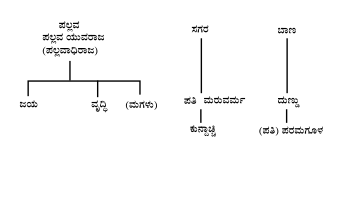
\includegraphics{"images/chap2/1.jpeg"}
\end{figure}

ಶ‍್ರೀಪುರುಷನ ಆಳ್ವಿಕೆಯಲ್ಲಿ, ಕುನ್ದಸತ್ತಿ ಅರಸನು ವಡಗೆರೆ ಮುನ್ನೂರನ್ನು ಆಳುತ್ತಿದ್ದನೆಂದು ಪೂರಿಗಾಲಿ ಶಾಸನದಲ್ಲಿ ಹೇಳಿದೆ.\endnote{ ಎಕ 7 ಮವ 122 ಪೂರಿಗಾಲಿ}\textbf{ }

\textbf{ ಒಂದನೇ ಮಾರಸಿಂಹ (ಯುವರಾಜ ಮಾರಸಿಂಹ) (796):} ಶ‍್ರೀಪುರುಷನ ನಂತರ ಪಟ್ಟಕ್ಕೆ ಬಂದ ಅವನ ಮಗ ಎರಡನೆಯ ಸೈಗೊಟ್ಟ ಶಿವಮಾರನ(788\enginline{–}816) ಶಾಸನಗಳು ಯಾವುವೂ ಜಿಲ್ಲೆಯಲ್ಲಿ ದೊರಕಿಲ್ಲ. ರಾಷ್ಟ್ರಕೂಟರೊಡನೆ ನಡೆಸಿದ ಯುದ್ಧದ ಪರಿಣಾಮವಾಗಿ ಸೈಗೊಟ್ಟ ಶಿವಮಾರನು ರಾಷ್ಟ್ರಕೂಟರ ಬಂಧಿಯಾಗಿದ್ದಾಗ, ಅವನ ಮಗ ಒಂದನೆಯ ಮಾರಸಿಂಹ ಎರೆಯಪ್ಪನು ತನ್ನನ್ನು ಯುವರಾಜನೆಂದು ಘೋಷಿಸಿಕೊಂಡಿದ್ದನು.\endnote{ ದೇವರಕೊಂಡಾ ರೆಡ್ಡಿ, ಡಾ॥. ಗಂಗ ಶಿಲ್ಪಕಲೆ, ಪುಟ 20} ಮಾರಸಿಂಹನು ರಾಷ್ಟ್ರಕೂಟರ ಅಧೀನದಲ್ಲಿ ಗಂಗಮಂಡಲಾಧಿಪತ್ಯವನ್ನು ಕ್ರಿ.ಶ. 796\enginline{–}97ರಲ್ಲಿ ವಹಿಸಿಕೊಂಡಿರಬಹುದು ಎಂದು ವಿದ್ವಾಂಸರು ಅಭಿಪ್ರಾಯ ಪಟ್ಟಿದ್ದಾರೆೆ.\endnote{ ಕರ್ನಾಟಕದ ಅರಸು ಮನೆತನಗಳು, ಎನ್​.ಲಕ್ಷ್ಮೀನಾರಾಯಣರಾವ್​, ಆರ್​.ಎಸ್​. ಪಂಚಮುಖಿ. ಪುಟ 151} ಮಾರಸಿಂಹ ಎರೆಯಪ್ಪನ ಅನುಮತದಿಂದ, ಕಲಿನೊಳಂಬಾದಿರಾಜ ಕೊಲ್ಲಿಯರಸನು ತನ್ನ ಮಗ ನಿಜರಾಮ ನಯಧೀರರೊಡ\-ಗೂಡಿ ತಿಪ್ಪೆರೂರು ಗ್ರಾಮವನ್ನು ಪೊನ್ನಡಿ ಎಂಬ ಬ್ರಾಹ್ಮಣನಿಗೆ ಬ್ರಹ್ಮದೇಯವಾಗಿ ನೀಡಿದನೆಂದು ಗಂಜಾಮ್ ಶಾಸನದಲ್ಲಿ ಹೇಳಿದೆ.\endnote{ ಎಕ 6 ಶ‍್ರೀಪ 66 ಗಂಜಾಂ 790} ಕಲಿನೊಳಂಬಾದಿ ರಾಜ ಕೊಲ್ಲಿಯರಸನು ಸಿಂಹಪೋತ ಕಲಿನೊಳಂಬಾದಿರಾಜನೆಂದು ವಿದ್ವಾಂಸರು ಗುರುತಿಸಿದ್ದಾರೆ.\endnote{ \engfoot{Krishna Murthy, Dr. M.S., The Nolambas, page 56,}} ಎರಡನೆಯ ಶಿವಮಾರನನ್ನು ರಾಷ್ಟ್ರಕೂಟರ ಧ್ರುವನು ಕ್ರಿ.ಶ.778ರ ಹೊತ್ತಿಗೆ ಸೆರೆಯಲ್ಲಿಟ್ಟಿದ್ದನು. ಆಗ ಶಿವಮಾರನ ಸಹೋದರನಾದ ದುಗ್ಗಮಾರನು ಸಿಂಹಾಸನವನ್ನು ಏರಲು ಪ್ರಯತ್ನಿಸಿದಾಗ, ಪೆರ್ಮಾನಡಿ ಶಿವಮಾರನ ಆದೇಶದ ಮೇರೆಗೆ, ಕಲಿನೊಳಂಬಾದಿರಾಜ ಸಿಂಹಪೋತನು, ದುಗ್ಗಮಾರನ ವಿರುದ್ಧ ಹೋರಾಡಿದ ವಿಚಾರ ದೊಡ್ಡ ಉಳುವರ್ತಿ ಶಾಸನದಿಂದ ತಿಳಿದುಬರುತ್ತದೆ. ಕೊಲ್ಲಿಪಲ್ಲವ ನೊಳಂಬನಿಗೆ ಚಾರುಪೊನ್ನೇರ, ನಿಜರಾಮ ಮತ್ತು ನಯಧೀರ ಎಂಬ ಮೂರು ಜನ ಗಂಡುಮಕ್ಕಳೂ, ಮಹಾದೇವಿ, ನೊಳಂಬ ಮಹಾದೇವಿ ಎಂಬ ಇಬ್ಬರು ಹೆಣ್ಣುಮಕ್ಕಳೂ ಇದ್ದರು.\endnote{ \engfoot{Krishna Murthy, Dr. M.S., The Nolambas, page17, 19, 56,57, }} ದುಗ್ಗಮಾರನು ಶಿವಮಾರನ ತಮ್ಮನೆಂದೂ, ಗಂಗವಾಡಿಯ ಸಿಂಹಾಸನಕ್ಕಾಗಿ ಅವನು ದಂಗೆ ಎದ್ದಾಗ ಶಿವಮಾರನ ಸಾಮಂತನಾದ ಸಿಂಹಪೋತನು ಶಿವಮಾರನ ನೆರವಿಗೆ ಬಂದು ದಂಗೆಯನ್ನು ಅಡಗಿಸಿದನೆಂದೂ ತಿಳಿದುಬರುತ್ತದೆ.\endnote{ ಕೃಷ್ಣರಾವ್​, ಎಂ.ವಿ., ಕರ್ನಾಟಕದ ಇತಿಹಾಸ ದರ್ಶನ, ಪುಟ 49}

ಬ್ರಹ್ಮಧೇಯವಾಗಿ ನೀಡಿದ ತಿಪ್ಪೆರೂರಿನ ಎಲ್ಲೆಯನ್ನು ಹೇಳುವಾಗ ಪಡುವ ಕಾವೇರಿಯ ಸೆಟ್ಟಿಗೆರೆ, ಕಳ್ಳರ್ವಾಡಿ, ಮುದುಗುಪ್ಪೆ ಗ್ರಾಮಗಳನ್ನು ಉಲ್ಲೇಖ ಮಾಡಿದೆ. ಸೆಟ್ಟಿಗೆರೆಯು ಇಂದು ಕಾವೇರಿಯ ಪಕ್ಕದಲ್ಲೇ ಇರುವ ಸೆಟ್ಟಿಹಳ್ಳಿ ಯಾಗಿರಬಹುದು, ಕಳ್ಳರ್ವಾಡಿಯು, ಇಂದಿನ ಕಳಸ್ತವಾಡಿ, ಮುದುಗುಪ್ಪೆಯು ಇಂದಿನ ದರಸಗುಪ್ಪೆಯಾಗಿರುವ ಸಾಧ್ಯತೆ ಇದೆ. ಆದುದರಿಂದ ಈ ಶಾಸನವು ಗಂಜಾಮ್ ಪರಿಸರದ್ದೆಂದು ಹೇಳಬಹುದು. 

\textbf{ಒಂದನೇ ರಾಚಮಲ್ಲ (816\general{\enginline{–}}843):} ಎರಡನೆಯ ಶಿವಮಾರನು ಬದುಕಿರುವಾಗಲೇ ಅವನ ಮಗ ಯುವರಾಜ ಮಾರಸಿಂಹನು ಮೃತನಾಗಿದ್ದನು. ಶಿವಮಾರನು ತನ್ನ ಎರಡನೆಯ ಮಗ ಒಂದನೆಯ ಪೃಥ್ವೀಪತಿಗೆ ಪಟ್ಟವನ್ನು ನೀಡದೇ, ತನ್ನ ತಮ್ಮ ವಿಜಯಾದಿತ್ಯನಿಗೆ ರಾಜ್ಯವನ್ನು ನೀಡಿದಾಗ, ಅವನು ರಾಜ್ಯವನ್ನು ಸ್ವೀಕರಿಸದೇ ತನ್ನ ಮಗ ಒಂದನೆಯ ರಾಜಮಲ್ಲನಿಗೆ ಪಟ್ಟಕಟ್ಟಿದನು.\endnote{ ಕರ್ನಾಟಕದ ಅರಸುಮನೆತನಗಳು, ಪುಟ 153, 154, ಕರ್ನಾಟಕದ ಸಂಕ್ಷಿಪ್ತ ಇತಿಹಾಸ, ಪುಟ 34} ಇವನಿಗೆ ಸತ್ಯವಾಕ್ಯ ಪೆರ್ಮಾನಡಿ ಎಂಬು ಬಿರುದು ಇತ್ತು. ನೊಳಂಬರ ಜೊತೆ ವೈವಾಹಿಕ ಸಂಬಂಧವನ್ನು ಮಾಡಿಕೊಂಡು ಸ್ನೇಹ ಸಾಧಿಸಿ,\endnote{ ಕೃಷ್ಣರಾವ್​ ಎಂ.ವಿ., ಕರ್ನಾಟಕದ ಇತಿಹಾಸ ದರ್ಶನ, ಪುಟ 52} ರಾಷ್ಟ್ರಕೂಟ ಸಾಮ್ರಾಜ್ಯದ ಅಂತಃಕಲಹದ ಪರಿಸ್ಥಿತಿಯನ್ನು ಉಪಯೋಗಿಸಿಕೊಂಡು ರಾಷ್ಟ್ರಕೂಟರ ಹಿಡಿತದಿಂದ ಬಿಡಿಸಿಕೊಂಡು ಸ್ವತಂತ್ರನಾಗಲು ಹವಣಿಸಿದನು. ಈ ಪ್ರಯತ್ನವನ್ನು ಹತ್ತಿಕ್ಕುವಂತೆ ಆಗ ರಾಷ್ಟ್ರಕೂಟರ ಚಕ್ರವರ್ತಿಯಾಗಿದ್ದ ಅಮೋಘವರ್ಷ ನೃಪತುಂಗನು ತನ್ನ ಪ್ರಬಲ ಸೇನಾನಿ ಬಂಕೆಯನಿಗೆ ಆದೇಶ ನೀಡಿದನು. ವೀರಬಂಕೆಯನು ಅಪಾರವಾದ ತನ್ನ ಸೇನೆಯೊಡಗೂಡಿ ಕಾವೇರಿ ನದಿಯವರೆಗೂ ದಂಡೆತ್ತಿಬಂದನು. ಬಂಕೆಯನು ಗಂಗರಾಜನನ್ನು ಕಾವೇರಿಯಿಂದ ಆಚೆಗೆ ಓಡಿಸಿದಂತೆ ಹೇಳಿಕೊಂಡಿದ್ದಾನೆ.\endnote{ ದೇವರಕೊಂಡಾರೆಡ್ಡಿ, ಡಾ॥, ಗಂಗರ ಶಿಲ್ಪಕಲೆ, ಪುಟ 20} ಚಿನಕುರಳಿ, ಇಂಗಲಗುಪ್ಪೆಯ ವೀರಗಲ್ಲುಗಳು ಈ ಆಕ್ರಮಣಕ್ಕೆ ಸಾಕ್ಷಿಯಾಗಿವೆ. 

ಸತ್ಯವಾಕ್ಯ ಪೆರ್ಮಾನಡಿಯ ಆಳ್ವಿಕೆಯಲ್ಲಿ ಬಮ್ಮ ಎಂಬುವವನು ತುರುಗೋಳಿನಲ್ಲಿ ಸತ್ತನೆಂದು ಚಿನಕುರಳಿಯ ವೀರಗಲ್ಲು ಶಾಸನದಿಂದ ತಿಳಿದುಬರುತ್ತದೆ.\endnote{ ಎಕ 6 ಪಾಂಪು 52 ಚಿನಕುರಳಿ} ಈ ತುರುಗೋಳು ರಾಷ್ಟ್ರಕೂಟರ ಆಕ್ರಮಣ ಕಾಲದಲ್ಲಿ ನಡೆದಿರಬಹುದು. ಚಿನಕುರಳಿಗೆ ಸಮೀಪದಲ್ಲೇ ಇರುವ ಇಂಗಲಗುಪ್ಪೆಯ ವೀರಗಲ್ಲಿನಲ್ಲಿ \textbf{“ಬಲ್ಲಹನ ಬೆಸದೊಳೆ ಬಂಕೆಯನು ದಳವಿಟ್ಟಿರಿದಲ್ಲಿ ತಳ್ಳಿಯದ ಘಣ್ಟಮ್ಮ ಊರಳಿವಿಲ್ಲಿ ಕಾದಿ ಸತ್ತ}”ನೆಂದು ಹೇಳಿದೆ. ಗಂಗರು ರಾಷ್ಟ್ರಕೂಟರ ಯುದ್ಧಕ್ಕೆ ಈ ವೀರಗಲ್ಲು ಪ್ರಮುಖ ಸಾಕ್ಷಿಯಾಗಿದೆ. ಆದರೆ ಅಮೋಘವರ್ಷನ ಕರೆಯ ಮೇರೆಗೆ, ರಾಷ್ಟ್ರಕೂಟ ಸಾಮ್ರಾಜ್ಯದಲ್ಲಿ ಉಂಟಾಗಿದ್ದ ಅರಾಜಕತೆಯನ್ನು ಅಡಗಿಸಲು ಬಂಕೇಶನು ಈ ದಾಳಿಯನ್ನು ಅರ್ಧಕ್ಕೇ ನಿಲ್ಲಿಸಿ ಹಿಂದಿರುಗಬೇಕಾಯಿತೆಂದು ತಿಳಿದುಬರುತ್ತದೆ.\endnote{ ಸೂರ್ಯನಾಥ ಕಾಮತ್​, ಡಾ॥, ಕರ್ನಾಟಕದ ಸಂಕ್ಷಿಪ್ತ ಇತಿಹಾಸ, ಪುಟ 59, ಕರ್ನಾಟಕದ ಇತಿಹಾಸ ದರ್ಶನ, ಪುಟ 53}

\textbf{ಒಂದನೇ ನೀತಿಮಾರ್ಗ ಎರೆಗಂಗ (843\general{\enginline{–}}870):} ಒಂದನೇ ರಾಚಮಲ್ಲನ ಮಗ ಒಂದನೇ ನೀತಿಮಾರ್ಗ ಎರೆಗಂಗನ ಕಾಲದಲ್ಲೂ ರಾಷ್ಟ್ರಕೂಟ ಗಂಗರ ಯುದ್ಧಗಳು ಮುಂದುವರಿದವು.\endnote{ ದೇವರಕೊಂಡಾರೆಡ್ಡಿ, ಡಾ॥, ಗಂಗರಶಿಲ್ಪಕಲೆ, ಪುಟ 21} ರಾಷ್ಟ್ರಕೂಟ ಅಮೋಘವರ್ಷನ ಸೇನಾನಿ ಬಂಕೇಶನು, ರಾಜಾರಮಡು ಎಂಬಲ್ಲಿ ನಡೆದ ಕದನದಲ್ಲಿ ನೀತಿಮಾರ್ಗನನ್ನು ಸೊಲಿಸಿದನು.\endnote{ ಅದೇ, ಪುಟ 20,} ರಾಜಾರಮಡು ಕದನದಲ್ಲಿ ಅಮೋಘವರ್ಷನ ಸೇನಾನಿ ಬಂಕೇಶನೇ ಸೋತನೆಂದು ಗಂಗರ ಶಾಸನಗಳಿಂದ ತಿಳಿದುಬರುತ್ತದೆ.\endnote{ ಕರ್ನಾಟಕದ ಸಂಕ್ಷಿಪ್ತ ಇತಿಹಾಸ, ಪುಟ 34–35, ಕರ್ನಾಟಕದ ಅರಸು ಮನೆತನಗಳು, ಪುಟ 157} ಕೊನೆಗೆ ಅಮೋಘವರ್ಷ ನೃಪತುಂಗನು ಗಂಗರ ಮೇಲಿನ ದ್ವೇಷವನ್ನು ಬದಿಗೊತ್ತಿ ಅವರೊಡನೆ ಸ್ನೇಹ ಹಾಗೂ ವೈವಾಹಿಕ ಸಂಬಂಧವನ್ನು ಬೆಳೆಸಿ ತನ್ನ ಮಗಳು ರೇವಕ್ಕ ನಿರ್ಮ್ಮಡಿಯನ್ನು ನೀತಿಮಾರ್ಗ ಎರೆಗಂಗನಿಗೆ ಕೊಟ್ಟು ವಿವಾಹ ಮಾಡಿದನು.\endnote{ ಗಂಗ ಶಿಲ್ಪಕಲೆ, ಪುಟ 21–22} ನೀತಿಮಾರ್ಗನಿಗೆ ಎರಡನೆಯ ರಾಚಮಲ್ಲ ಮತ್ತು ಬೂತುಗ ಎಂಬ ಇಬ್ಬರು ಮಕ್ಕಳಿದ್ದರು. ಈತನ ಎರಡು ಶಾಸನಗಳು ಜಿಲ್ಲೆಯಲ್ಲಿ ದೊರಕಿವೆ. ಪೂರ್ಣವಾಗಿ ತ್ರುಟಿತವಾಗಿರುವ ರಾವಂದೂರಿನ ಶಾಸನದಲ್ಲಿ ಇವನ ಹೆಸರನ್ನು ಬಿಟ್ಟರೆ ಬೇರೆ ಯಾವ ವಿವರಗಳೂ ತಿಳಿದುಬರುವುದಿಲ್ಲ.\endnote{ ಎಕ 7 ಮಳವಳ್ಳಿ 15 ರಾವಂದೂರು 8–9 ನೇ ಶ.} ಎಮ್ಮಳ್ದಕ್ಕೆ ಗ್ರಾಮವನ್ನು ನೆಲ್ಲ ಕೂಳಣವಾಗಿ (ಭತ್ತ ಬೆಳೆಯುವ ಗದ್ದೆಯನ್ನು) ದತ್ತಿಯಾಗಿ ಬಿಟ್ಟ ವಿಚಾರ ಯಮ್ಮದೂರು ಶಾಸನದಿಂದ ತಿಳಿದುಬರುತ್ತದೆ. \endnote{ ಎಕ 7 ಮಳವಳ್ಳಿ 135 ಯಮ್ಮದೂರು 9ನೇ ಶ.} ಈ ಶಾಸನ ಬಹುಶಃ ಇಮ್ಮಡಿ ನೀತಿಮಾರ್ಗನೇ ಆದ ಎರೆಗಂಗನದು ಎಂದು ಹೇಳಲಾಗಿದೆ.\endnote{ ಅದೇ} ಆದರೆ ಇಮ್ಮಡಿ ನೀತಿಮಾರ್ಗನಿಗೆ ಪೆರ್ಮಾನಡಿ ಎಂಬ ಬಿರುದಿಲ್ಲ. ಯಮ್ಮದೂರು ಶಾಸನದ ಒಕ್ಕಣೆಯೂ, ಒಂದನೇ ನೀತಿಮಾರ್ಗ ಎರೆಗಂಗನು ಮರಣಹೊಂದಿದ ವಿಚಾರವನ್ನು ಹೇಳುವ ದೊಡ್ಡಹುಂಡಿ ಶಾಸನದ ಲಿಪಿ ಹಾಗೂ ಒಕ್ಕಣೆ ಒಂದೇ ಆಗಿದೆ\endnote{ ಎಕ 5 ತಿ.ನ.ಪುರ 257 ದೊಡ್ಡಹುಂಡಿ 10ನೇ ಶ.}. ದೊಡ್ಡಹುಂಡಿ ರಾವಂದೂರಿಗೆ ಸಮೀಪದಲ್ಲೇ ಇರುವ ಊರು. ಆದುದರಿಂದ ಯಮ್ಮದೂರು ಶಾಸನೋಕ್ತ ನೀತಿಮಾರ್ಗನು ಮೊದಲನೆಯ ನೀತಿಮಾರ್ಗನೇ ಆಗಿದ್ದಾನೆಂದು ಹೇಳಬಹುದು. 

\textbf{ಸತ್ಯವಾಕ್ಯ ಇಮ್ಮಡಿ ರಾಜಮಲ್ಲ (870\general{\enginline{–}}907) ಮತ್ತು ಒಂದನೆಯ ಬೂತುಗ: } ಸತ್ಯವಾಕ್ಯ ಬಿರುದಾಂಕಿತ ಇಮ್ಮಡಿ ರಾಚಮಲ್ಲನು ಸು.870 ರಲ್ಲಿ ಪಟ್ಟಕ್ಕೆ ಬಂದನು. ಇವನು ತನ್ನ ತಮ್ಮ ಒಂದನೆಯ ಬೂತುಗನೊಂದಿಗೆ, ಅನಂತರ ಅವನ ಮಗ ಎರೆಯಪ್ಪನೊಂದಿಗೆ ದೀರ್ಘಕಾಲ ರಾಜ್ಯಭಾರ ಮಾಡಿದನು. ಅಮೋಘವರ್ಷನು ತನ್ನ ಮಗಳು ಚಂದ್ರೊಬ್ಬಲಬ್ಬೆಯನ್ನು ಒಂದನೇ ಬೂತುಗನಿಗೆ ಕೊಟ್ಟು ವಿವಾಹ ಮಾಡಿದನು.\endnote{ ಅದೇ, ಪುಟ 21, ಕರ್ನಾಟಕದ ಸಂಕ್ಷಿಪ್ತ ಇತಿಹಾಸ, ಪುಟ 35} ರಾಜಮಲ್ಲ ಪೆರ್ಮಾನಡಿಯು ರಾಜ್ಯವಾಳುತ್ತಿದ್ದಾಗ ಬೂತರಸರು ಯುವರಾಜ ಪದವಿಯಲ್ಲಿ ಕೊಂಗಾಳ್ನಾಡು, ಪೂನಾಡು(ಪುನ್ನಾಡು)ಗಳನ್ನು ಆಳುತ್ತಿದ್ದನೆಂದು ಹುಸಕೂರು ಶಾಸನದಿಂದ ತಿಳಿದುಬರುತ್ತದೆ.\endnote{ ಎಕ 3 ನಂಜನಗೂಡು 385 ಹುಸಕೂರು 871} ಬೂತುಗನು ತನ್ನ ಅಣ್ಣನಿಗಿಂತ ಮೊದಲೇ ಮೃತನಾದನು. ಆಗ ಇಮ್ಮಡಿ ರಾಚಮಲ್ಲನು ಅವನ ಮಗ ಎರೆಗಂಗ ಅಥವಾ ಎರೆಯಪ್ಪರಸನನ್ನು ಯುವರಾಜನನ್ನಾಗಿ ಮಾಡಿದನು. “ಶ‍್ರೀಮತ್​ ಪೆರ್ಮಾನಡಿಗಳು ಹಾಗೂ ಎರೆಯಪ್ಪರಸರು” ಇಬ್ಬರೂ ಇದ್ದು ಚಾಗಿಪೆರ್ಮಾನಡಿಗಳ ಕೆಲ್ಲಬಸದಿಯ ಚರಪಿಗೆ ಕೊಮಾರಸೇನ ಭಟಾರರಿಗೆ ದತ್ತಿಯನ್ನು ಬಿಟ್ಟರೆಂದು ಕ್ಯಾತನಹಳ್ಳಿ ಶಾಸನದಿಂದ ತಿಳಿದುಬರುತ್ತದೆ.\endnote{ ಎಕ 6 ಪಾಂಪು 16 ಕ್ಯಾತನಹಳ್ಳಿ 9–10 ಅ} ಎರೆಯಪ್ಪನು ಕೊಂಗಳ್ನಾಡು8000, ನುಗುನಾಡು, ನವಲೆನಾಡು ಮತ್ತು ಇತರ ಪ್ರಾಂತಗಳನ್ನು ಆಳುತ್ತಿದ್ದನು.\endnote{ ಕರ್ನಾಟಕ ಇತಿಹಾಸ ದರ್ಶನ, ಪುಟ 55. ಪ್ರೊ: ಎಂ.ವಿ.ಕೃಷ್ಣರಾವ್​,} ಕ್ಯಾತನಹಳ್ಳಿ ಶಾಸನದಿಂದ ಈತ ಕಳ್ಬಪ್ಪು ನಾಡನ್ನೂ ಆಳುತ್ತಿದ್ದನೆಂದು ಊಹಿಸಬಹುದು. ಇದೇ ಕಾಲಕ್ಕೆ ಸೇರಿರಬಹುದಾದ ನೆಲಮನೆ ಶಾಸನವು ಸತ್ಯವಾಕ್ಯ ಇಮ್ಮಡಿ ರಾಚಮಲ್ಲನ ಹೆಸರಿನಲ್ಲಿ ಮಾತ್ರ ಹೊರಟಿದೆ. ಕ್ಯಾತನಹಳ್ಳಿ ಶಾಸನದಲ್ಲಿ ನೀಡಿರುವ ಬಿರುದಾವಳಿಗಳನ್ನು ಈ ಶಾಸನದಲ್ಲಿಯೂ ಕೂಡಾ ನೀಡಲಾಗಿದೆ. ಇಲ್ಲಿಯೂ ಕೂಡಾ ಜೈನಬಸದಿಗೆ ನೆಲ್ಲಕೂಳಣ ಅಂದರೆ ಬತ್ತದ ಗದ್ದೆಯನ್ನು ದತ್ತಿಯಾಗಿ ಬಿಡಲಾಗಿದೆ.\endnote{ ಎಕ 6 ಪಾಂಪು 94 ನೆಲಮನೆ 9–10 ನೇ ಶತಮಾನ}

ಇಮ್ಮಡಿ ರಾಚಮಲ್ಲನು ತನ್ನ ಆಳ್ವಿಕೆಯ 27ನೆಯ ವರ್ಷದಲ್ಲಿ, ಅಂದರೆ ಕ್ರಿ.ಶ.896\enginline{–}97ರಲ್ಲಿ, ದೇವಾಲಯ ಒಂದಕ್ಕೆ ನೊಳಂಬನು ಬಿಟ್ಟ ದತ್ತಿಯನ್ನು ಮುಂದುವರಿಸಿರುವ ವಿಷಯವು ತಾಯಲೂರು ಶಾಸನದಿಂದ ತಿಳಿಯುತ್ತದೆ.\endnote{ ಎಕ 7 ಮವ 57 ತಾಯಲೂರು 897} ಈ ಶಾಸನವು ನೊಳಂಬ ಅರಸನ ಶಾಸನದ ಹಿಂಭಾಗದಲ್ಲಿಯೇ ಕಂಡರಿಸಲ್ಪಟ್ಟಿದೆ. ಈ ಕಾಲಕ್ಕೆ ಗಂಗರ ಸಾಮಂತನಾಗಿದ್ದ ನೊಳಂಬಾದಿರಾಜ ಮಹೇಂದ್ರನು, ರಾಚಮಲ್ಲ ಮತ್ತು ಬೂತುಗರ ನಡುವಿನ ಭಿನ್ನಾಭಿಪ್ರಾಯವನ್ನು ಉಪಯೋಗಿಸಿಕೊಂಡು ಸ್ವತಂತ್ರನಾಗಲು ಹವಣಿಸಿ ಗಂಗವಾಡಿಯ ಮೇಲೆ ಆಕ್ರಮಣ ಮಾಡುತ್ತಾ ಗಂಗರ ರಾಜಧಾನಿ ತಲಕಾಡಿನವರೆಗೂ ಬಂದನು. ತಲಕಾಡಿಗೆ ಅನತಿದೂರದಲ್ಲಿರುವ ತಾಯಲೂರಿನಲ್ಲಿರುವ ಒಂದು ದೇವಾಲಯಕ್ಕೆ ತನ್ನ ಹೆಸರಿನಲ್ಲಿ ದತ್ತಿಯನ್ನು ನೀಡಿದನು.\endnote{ ಎಕ 7 ಮವ 57 ತಾಯಲೂರು 895} ಆದರೆ ರಾಚಮಲ್ಲನು ನೊಳಂಬರ ಮಹೇಂದ್ರನನ್ನು ಹಿಮ್ಮೆಟ್ಟಿಸಿ, ಈ ದೇವಾಲಯಕ್ಕೆ ನೊಳಂಬ ಅರಸನು ನೀಡಿದ್ದ ದತ್ತಿಯನ್ನು ಮುಂದುವರಿಸಿದನು. ಗಂಗ ನೊಳಂಬರ ಇತಿಹಾಸದ ದೃಷ್ಟಿಯಿಂದ ಈ ಶಾಸನವು ಬಹಳ ಮಹತ್ವದ್ದಾಗಿದೆ. ರಾವಂದೂರಿನ ಶಾಸನದಲ್ಲೂ ಕೂಡಾ ನೊಳಂಬನ ಸಮ್ಮುಖದಲ್ಲಿ ಬಿತ್ತುವಾಟಕ್ಕೆ ಭೂಮಿಯನ್ನು ಬಿಡಲಾಯಿತೆಂದು ಹೇಳಿದೆ.\endnote{ ಎಕ 7 ಮವ 17 ರಾವಂದೂರು 9ನೇ ಶ.} ಈ ಶಾಸನದಲ್ಲಿ ಉಕ್ತನಾದ ನೊಳಬಂನೂ ಕೂಡಾ ಮಹೇಂದ್ರನೇ ಆಗಿದ್ದು ಈ ಶಾಸನವೂ ಕೂಡಾ ತಾಯಲೂರಿನ ಶಾಸನದ ಕಾಲಕ್ಕೇ ಸೇರಿದೆ ಎಂದು ಊಹಿಸಬಹುದು.

ಎರಡನೆಯ ರಾಜಮಲ್ಲನ ಆಳ್ವಿಕೆಯ 34ನೇ ವರ್ಷದಲ್ಲಿ, ಅಂದರೆ ಕ್ರಿ.ಶ. 904ರಲ್ಲಿ, ಮತಿಸಾಗರ ಭಟಾರರ ಆಜ್ಞೆಯಂತೆ ಪೆರ್ಬಾಣನಹಳ್ಳಿಯನ್ನು ಕೊಂಡ ಶ‍್ರೀ ಕೇಸಿಗ ಎಂಬುವವನು ತಲೆನೆರೆಯಲ ಕಟ್ಟೆಯನ್ನು ಕಟ್ಟುವುದಕ್ಕೆ ಕೆಲವು ದತ್ತಿಗಳನ್ನು ಬಿಟ್ಟನೆಂದು ರಾಂಪುರ ಶಾಸನದಿಂದ ತಿಳಿದುಬರುತ್ತದೆ.\endnote{ ಎಕ 6 ಶ‍್ರೀಪ 85 ರಾಮಪುರ 904–05} ಈ ದತ್ತಿಯನ್ನು ಬಿಡುವಾಗ ಅಣ್ನಯ್ಯ, ದೇವಕುಮಾರ ಮತ್ತು ದೋರ ಇವರು ಇದ್ದರೆಂದು ಶಾಸನ ತಿಳಿಸುತ್ತದೆ. ಈ ವೇಳೆಗೆ ರಾಷ್ಟ್ರಕೂಟರು ಮತ್ತು ಗಂಗರ ನಡುವೆ ಮಧುರವಾದ ಸಂಬಂಧ ಇದ್ದು ದೋರನು ರಾಷ್ಟ್ರಕೂಟರ ಅಧಿಕಾರಿಯಾಗಿದ್ದಿರಬಹುದೆಂದು ಹೆಸರಿನ ಆಧಾರದ ಮೇಲೆ ಊಹಿಸಬಹುದು. ಸತ್ಯವಾಕ್ಯ ರಾಚಮಲ್ಲನು ಕ್ರಿ.ಶ.907ರಲ್ಲಿ ಕೊಂಬಾಳೆಯಲ್ಲಿ ಕೊನೆಯುಸಿರೆಳೆಯುತ್ತಾನೆ.\endnote{ ದೇವರಕೊಂಡಾರೆಡ್ಡಿ, ಡಾ॥, ಗಂಗ ಶಿಲ್ಪಕಲೆ, ಪುಟ 23}

ಸತ್ಯವಾಕ್ಯ ಪೆರ್ಮಾನಡಿಯ ತ್ರುಟಿತ ಶಾಸನವೊಂದು ಪಾಂಡವಪುರ ತಾಲ್ಲೂಕಿನ ಮಲ್ಲಿಗೆರೆ ಗ್ರಾಮದ ಹೆಬ್ಬಾಗಿಲಿ ಬಳಿ ಇದ್ದು, ಜೈನಬಸದಿಗೆ ನೀಡಿರುವ ದತ್ತಿಯ ವಿಚಾರವನ್ನು ತಿಳಿಸುತ್ತದೆ. ಇದು ಬಹುಶ: ರಾಜಮಲ್ಲನ ಕೊನೆಯ ವರ್ಷದ ಶಾಸನಗಳಲ್ಲಿ ಒಂದು.\endnote{ ಎಕ 6 ಪಾಂಪು 47 ಮಲ್ಲಿಗೆರೆ 906–07} ರಾಜಮಲ್ಲನು ಅನೇಕ ಜೈನಬಸದಿಗಳಿಗೆ, ಹಲವಾರು ಬ್ರಾಹ್ಮಣ ವಿದ್ವಾಂಸರಿಗೆ ದಾನ ದತ್ತಿಗಳನ್ನು ನೀಡಿದನು. ಜನರು ಸತ್ಕಾರ್ಯನಿರತವಾಗುವಂತೆ ಮಾಡಿದನು ಎಂದು ವಿದ್ವಾಂಸರು ಹೇಳಿರುವುದನ್ನು ಈ ಶಾಸನಗಳು ಸಮರ್ಥಿಸುತ್ತವೆ.\endnote{ ಕರ್ನಾಟಕ ಇತಿಹಾಸ ದರ್ಶನ, ಪ್ರೊ: ಎಂ.ವಿ. ಕೃಷ್ಣರಾವ್​, ಪುಟ 55}

\textbf{ಎರಡನೆಯ ನೀತಿಮಾರ್ಗ ಎರೆಗಂಗ– ಎರೆಯಪ್ಪ (907\general{\enginline{–}}920): } ಎರಡನೇ ರಾಜಮಲ್ಲನ ಜೊತೆ ಜಂಟಿಯಾಗಿ ಆಳ್ವಿಕೆ ನಡೆಸುತ್ತಿದ್ದ ಒಂದನೆಯ ಬೂತುಗನ ಮರಣಾನಂತರ ಅವನ ಮಗ ಎರಡನೆಯ ನೀತಿಮಾರ್ಗ ಎರೆಗಂಗನು ಕ್ರಿ.ಶ.886ರಲ್ಲಿ ಪಟ್ಟಕ್ಕೆ ಬಂದನು.\endnote{ ದೇವರಕೊಂಡಾರೆಡ್ಡಿ, ಡಾ॥, ಗಂಗ ಶಿಲ್ಪಕಲೆ, ಪುಟ 22} ಇವನಿಗೆ ನೀತಿಮಾರ್ಗ ಪೆರ್ಮಾನಡಿ, ನೀತಿಮಾರ್ಗ ರಣವಿಕ್ರಮಾರ್ಯ ಎಂಬ ಬಿರುದು ಇತ್ತು.\endnote{ ಎಕ 5 ಕೃನಾ 105 ಗಳಿಗೆಕೆರೆ, ಕ್ರಿ.ಶ. 9ನೇ ಶತಮಾನ.} ಪಟ್ಟಕ್ಕೆ ಬಂದ ನಂತರ ಎರೆಯಪ್ಪರಸನೆಂಬ ಬಿರುದನ್ನು ಧರಿಸಿದನು\textbf{. }ಎರೆಯಪ್ಪರಸನು ಕೊಂಗಾಳ್ನಾಡಿನಲ್ಲಿ ವೀರನೊಬ್ಬನಿಗೆ ಬಾಳ್ಗಚ್ಚನ್ನು ಕೊಟ್ಟ ವಿಚಾರ, ಕೃಷ್ಣರಾಜಪೇಟೆ ತಾಲ್ಲೂಕು, ಹೊನ್ನೇನಹಳ್ಳಿ ಶಾಸನದಿಂದ ತಿಳಿದುಬರುತ್ತದೆ.\endnote{ ಎಕ 6 ಕೃಪೇ 20 ಹೊನ್ನೇನಹಳ್ಳಿ} ಹೊನ್ನೇನಹಳ್ಳಿಯು ಕೊಂಗಾಳ್ನಾಡು ಪ್ರದೇಶದಲ್ಲಿಯೇ ಇದೆ. ಈತನು ಕ್ರಿ.ಶ.907 ರಲ್ಲಿ ಪಟ್ಟಕ್ಕೆ ಬಂದರೂ, ಅದಕ್ಕೆ ಮುಂಚೆ ಅಂದರೆ ಕ್ರಿ.ಶ.887 ರಿಂದಲೇ ಯುವರಾಜನಾಗಿ ಕೊಂಗಾಳ್ನಾಡು–8000 ವನ್ನು, ಬೂತುಗನರಸಿ ಪರಮಬ್ಬೆಯು ಕೂರ್ಗಲ್ಲನ್ನು ಆಳುತ್ತಿದ್ದಳೆಂದು ತಿಳಿದುಬರುತ್ತದೆ.\endnote{ ಎಕ 4 ಹುಣಸೂರು 8 ಕೂರಗಲ್ಲು}

ಅಕಾಲವರ್ಷ ಇಮ್ಮಡಿ ಕೃಷ್ಣನು ನೊಳಂಬರ ಒಂದನೆಯ ಮಹೇಂದ್ರ ಮತ್ತು ಅವನ ಮಗ ಅಯಪ ದೇವ ಇವರುಗಳನ್ನು ಸೋಲಿಸಿ ನೊಳಂಬವಾಡಿಯನ್ನು ಆಕ್ರಮಿಸಿಕೊಂಡು ಗಂಗವಾಡಿಯೊಳಕ್ಕೆ ನುಗ್ಗಿ ಮಣ್ಣೆಯಲ್ಲಿ ಪ್ರಚಂಡ ದಂಡನಾಯಕ\break ದಾಮಪಯ್ಯನೆಂಬುವನನ್ನು ಅಧಿಕಾರಿಯಾಗಿ ನೇಮಿಸಿದ್ದನು.\endnote{ ಎಕ 24 ತುಮಕೂರು 26 ಚಿಕ್ಕಸಾರಂಗಿ 903, ಕರ್ನಾಟಕದ ಅರಸುಮನೆತನಗಳು, ಪುಟ 166, \engfoot{The Nolambas, pp.98}} ಈ ಸನ್ನಿವೇಶದಲ್ಲಿ ರಾಷ್ಟ್ರಕೂಟರ ಸೇನೆಯು ಕೆಂಬೊಳಲನ್ನು ಮುತ್ತಿದಾಗ ಇದುಳೆಯನ್ನು ಬೀಳವೃತ್ತಿಯಿಂದ ಆಳುತ್ತಿದ್ದ ಆರಂಭಲ್ಲನು, ನೀತಿಮಾರ್ಗನ ಬೆಸದಿಂದ, ಬಲ್ಲಹನ ಅಂದರೆ ರಾಷ್ಟ್ರಕೂಟರ ಇಮ್ಮಡಿ ಕೃಷ್ಣನ ದಂಡನ್ನು ಪಳಿಯು..ಳನ ದಂಡನಾಯಕತ್ವದಲ್ಲಿ ಎದುರಿಸಿದಾಗ ತ..ಳಿಯಣ್ಣ ನೆಂಬುವವನು ಕಾದಿ ಮಡಿಯುತ್ತಾನೆ. ಅವನಿಗೆ ನಿಡುವುಟೆಯನ್ನು ಕಲ್ನಾಡಾಗಿ ನೀಡಲಾಯಿತು.\endnote{ ಎಕ 7 ನಾಮಂ 127 ಕಾರಬಯಲು 10ನೇ ಶ., ಎಕ 7 ಪೀಠಿಕೆ, ಪುಟ \engfoot{xlvii}

\engfoot{Sheik Ali, Dr.B., History of the Western Gangas, pp. 115, }} ನಿಡುವುಟೆಯು ಕೆಂಬಾಳಿಗೆ ಸಮೀಪ ಇರುವ ನಿಡುವೊಳಲಾಗಿರಬಹುದು. ಕೆಂಬೊಳಲು ಯುದ್ಧವು ಒಂದನೇ ರಾಚಮಲ್ಲನ ಕಾಲದಲ್ಲಿ ನಡೆದಿರಬಹುದೆಂದು ದೇವರಕೊಂಡಾರೆಡ್ಡಿಯವರು ಊಹಿಸಿದ್ದಾರೆ.\endnote{ ದೇವರಕೊಂಡಾರೆಡ್ಡಿ, ಡಾ॥, ಗಂಗ ಶಿಲ್ಪಕಲೆ, ಪುಟ 20}

ಗಂಗರ ಮಾಂಡಲಿಕನೂ ಮತ್ತು ಸೇನಾಧಿಪತಿಯೂ ಆಗಿದ್ದ, ಸಗರ ಕುಲದ ಮಣಲೆಯರನು (ಮಣಲೇರ, ಮನಾಲರ) ಕನಕಗಿರಿ ತೀರ್ಥದ ಮೇಲೆ ಬಸದಿಯನ್ನು ಮಾಡಿಸಿ, ಅದಕ್ಕೆ ತಿಪ್ಪೆಯೂರಿನ ಕೆಲವು ತೆರಿಗೆಗಳನ್ನು, ಅರಸರ ಅಧ್ಯಕ್ಷತೆಯಲ್ಲಿ, ಅಂದರೆ ನೀತಿಮಾರ್ಗ್ಗ ಪೆರ್ಮಾನಡಿಯ ಸಮ್ಮುಖದಲ್ಲಿ, ಕನಕಸೇನ ಭಟಾರರಿಗೆ ದತ್ತಿ ಬಿಟ್ಟನೆಂದು ಕೂಲಿಗ್ಗೆರೆ ಶಾಸನವು ತಿಳಿಸುತ್ತದೆ.\endnote{ ಎಕ 7 ಮ 100 ಕೂಲಿಗ್ಗೆರೆ 916–17}

ಇಮ್ಮಡಿ ನೀತಿಮಾರ್ಗನಿಗೆ, ನರಸಿಂಹ (ಸತ್ಯವಾಕ್ಯ ಬೀರ ಪೆರ್ಮಾನಡಿ), ರಾಚಮಲ್ಲ(ನೀತಿಮಾರ್ಗ), ಪಾಂಬಬ್ಬೆ, ಇಮ್ಮಡಿ ಬೂತುಗ(ಸತ್ಯವಾಕ್ಯ) ಎಂಬ ನಾಲ್ವರು ಮಕ್ಕಳಿದ್ದರು. ಕ್ರಿ.ಶ.920ರ ಶಾಸನದಲ್ಲಿ ಸತ್ಯವಾಕ್ಯ ಪೆರ್ಮಾನಡಿಯ ಉಲ್ಲೇಖವಿದ್ದು, ಈತನು ಅಂತ್ಯಕಾಲದಲ್ಲಿ ಅಧಿಕಾರಕ್ಕೆ ಬಂದಿರಬಹುದು. ಇಲ್ಲಿಂದ ಸುಮಾರು 930ರವರೆಗೆ ಗಂಗರ ಚಟುವಟಿಕೆಗಳ ಚಿತ್ರಣ ಸ್ಪಷ್ಟವಾಗಿ ಕಾಣಿಸುವುದಿಲ್ಲವೆಂದು ವಿದ್ವಾಂಸರು ಅಭಿಪ್ರಾಯ ಪಟ್ಟಿದ್ದಾರೆ.\endnote{ ದೇವರಕೊಂಡಾರೆಡ್ಡಿ, ಡಾ॥, ಗಂಗ ಶಿಲ್ಪಕಲೆ, ಪುಟ 23}

\textbf{ ಮೂರನೆಯ ರಾಜಮಲ್ಲ (933\general{\enginline{–}}38):} ಎರಡನೆಯ ನೀತಿಮಾರ್ಗನ ನಂತರ ಅವನ ಹಿರಿಯ ಮಗ ಮೂರನೆಯ ರಾಚಮಲ್ಲನು ಪಟ್ಟಕ್ಕೆ ಬಂದು, ತನ್ನ ತಮ್ಮ ಎರಡನೆಯ ಬೂತುಗನನ್ನು ಯುವರಾಜನನ್ನಾಗಿ ಮಾಡಿದನು. ಇತ್ತ ರಾಷ್ಟ್ರಕೂಟರ ಮೂರನೆಯ ಇಂದ್ರನು (914\enginline{–}929) ಪಟ್ಟಕ್ಕೆ ಬಂದನು. ಇವನ ಕಾಲದಲ್ಲಿ ರಾಷ್ಟ್ರಕೂಟರು ಗಂಗವಾಡಿಯ ಮೇಲೆ ಆಕ್ರಮಣ ಮಾಡಲಿಲ್ಲ. ಮೂರನೆಯ ಇಂದ್ರನಿಗೆ ಬದ್ದೆಗ ಅಥವಾ ಮೂರನೆಯ ಅಮೋಘವರ್ಷ ಎಂಬ ಮಲತಮ್ಮನಿದ್ದನು. ಈ ಬದ್ದೆಗನ ಮಗಳು ರೇವಕ ನಿಮ್ಮಡಿಯನ್ನು ಮೂರನೆಯ ರಾಚಮಲ್ಲನ ತಮ್ಮ ಎರಡನೆಯ ಬೂತುಗನಿಗೆ ವಿವಾಹ ಮಾಡಿಕೊಡಲಾಗಿತ್ತು. ಈ ವೈವಾಹಿಕ ಸಂಬಂಧದಿಂದ ಗಂಗರಿಗೂ ರಾಷ್ಟ್ರಕೂಟರಿಗೂ ಇದ್ದ ವೈರತ್ವವು ಹೋಗಿ ಮತ್ತೆ ಸ್ನೇಹ ಉಂಟಾಯಿತು. ಗಂಗವಾಡಿಯ ಸಿಂಹಾಸನಕ್ಕಾಗಿ ನಡೆದ ದಾಯಾದಿ ಕಲಹದಲ್ಲಿ, ಇಮ್ಮಡಿ ಬೂತುಗನು, ರಾಜಮಲ್ಲನನ್ನು ಕೊಂದುಹಾಕಿದ ಗಂಗವಾಡಿಯ ಅಧಿಪತಿಯಾದನೆಂಬ ವಿಚಾರ ಆತಕೂರು ಶಾಸನದಿಂದ ತಿಳಿದುಬರುತ್ತದೆ.\endnote{ ಎಕ 7 ಮದ್ದೂರು 42 ಆತಕೂರು 949–50}

\textbf{ ಇಮ್ಮಡಿ ಬೂತುಗ (938\general{\enginline{–}}961):} ಇಮ್ಮಡಿ ನೀತಿಮಾರ್ಗನ ಮಗ ಹಾಗೂ ಮೂರನೆಯ ರಾಜಮಲ್ಲನ ತಮ್ಮ ಎರಡನೇ ಬೂತುಗ. ಇವನ ಕಾಲದಲ್ಲಿ ಚೋಳರು ಗಂಗವಾಡಿಯ ಮೇಲೆ ಆಕ್ರಮಣ ಮಾಡತೊಡಗಿದರು. ಗಂಗರ ಮತ್ತೊಂದು \textbf{ಶಾಖೆಯ ಎರಡನೆಯ ಪೃಥ್ವೀಪತಿಯು} ಇದಕ್ಕೆ ಸಹಾಯಕನಾಗಿದ್ದನು. ಬಹುಶಃ ಈ ಸನ್ನಿವೇಶದಲ್ಲಿ ನಡೆದ ಯುದ್ಧದಲ್ಲಿ, ಎರಡನೆಯ ಬೂತುಗನು ತನ್ನ ಸೇನಾಧಿಪತಿ ಮಣಲೇರನ ಜೊತೆ ಕುಣಿಂಗಲವೂರಿನಲ್ಲಿ (ಕುಣಿಗಲ್​), ಕೊಂತದ ನರಗ ಎನ್ನುವವನ ಜೊತೆ ನಡೆಸಿದ ಹೋರಾಟದಲ್ಲಿ, ಎರೆಯಂಗನೆಂಬ ವೀರನು ಮೃತಪಟ್ಟಾಗ, ಅವನ ವೇಳೆಯ (ವೇಳೆವಾಳಿ) ಎಬ್ಬೆಬಸವನು ತಲೆಯನ್ನು ಕಡಿದುಕೊಂಡನೆಂದು ಕಲ್ಕುಣಿಯ ಶಾಸನದಲ್ಲಿ ಹೇಳಿದೆ.\endnote{ ಎಕ 7 ಮವ 141 ಕಲ್ಕುಣಿ 10ನೇ ಶ.}

ಮೂರನೆಯ ಕೃಷ್ಣನು ಗಂಗರ ಇಮ್ಮಡಿ ಬೂತುಗನ ಸಹಾಯದಿಂದ ತನ್ನ ಪ್ರತಿಸ್ಪರ್ಧಿಗಳಾಗಿದ್ದ ಚೋಳರ ಮೇಲೆ ದಂಡೆತ್ತಿ ಹೋದನು. ಚೋಳ ಪರಾಂತಕನ ಮಗ ಯುವರಾಜ ರಾಜಾದಿತ್ಯನೂ ತೊಂಡೈಮಂಡಲಮ್ ಕೋಟೆಯಲ್ಲಿ ಸೇನೆಯೊಡನೆ ಬೀಡುಬಿಟ್ಟು ಗಂಗವಾಡಿಯ ಮೇಲೆ ಆಕ್ರಮಣ ನಡೆಸಲು ಸಿದ್ಧನಾದನು. ತಕ್ಕೋಲಂನಲ್ಲಿ ನಡೆದ ಈ ಯುದ್ಧದ ಭೀಕರತೆಯನ್ನು ಹಾಗೂ ಚೋಳರ ರಾಜಾದಿತ್ಯನ ಸಾವು ಹೇಗಾಯಿತೆಂಬುದನ್ನು ಸಮಕಾಲೀನವೂ ವಿಶ್ವಾಸಾರ್ಹವೂ ಆದ ಮದ್ದೂರು ತಾಲ್ಲೂಕಿನ ಆತಕೂರು ಶಾಸನವು ಒದಗಿಸುತ್ತದೆ. ತಕ್ಕೋಲಂ ಯುದ್ಧದ ನಂತರ ಕೃಷ್ಣನು ತನ್ನ ರಾಜ್ಯಕ್ಕೆ ಹಿಂದಿರುಗುತ್ತಿದ್ದ ಸಮಯದಲ್ಲಿ ಈ ಶಾಸನವನ್ನು ಹೊರಡಿಸಲಾಗಿದೆ.\endnote{ ಎಕ 7 ಮ 42 ಆತಕೂರು 949–50}ತಕ್ಕೋಲಮ್ ಯುದ್ಧವು ಕ್ರಿ.ಶ.948\enginline{–}49ರಲ್ಲಿ ನಡೆದಿರಬಹುದೆಂದು ಊಹಿಸಲಾಗಿದೆ.\endnote{ ದೇವರಕೊಂಡಾರೆಡ್ಡಿ, ಗಂಗ ಶಿಲ್ಪಕಲೆ, ಪುಟ 24}

ಯುದ್ಧರಂಗದಲ್ಲಿ ಬೂತುಗನು ಚೋಳರ ರಾಜಾದಿತ್ಯನನ್ನು “ಬಿಸುಗೆಯ ಕಳನಾಗಿ” ಅಂದರೆ ಅವನು ಕುಳಿತಿದ್ದ ಆನೆಯ ಅಂಬಾರಿಯ ಮೇಲಕ್ಕೆ ನೆಗೆದು, ಅದರ ಮೇಲೆ ನಿಂತು ಯುದ್ಧಮಾಡಿ ಕೊಂದನೆಂದು, ಈ ಸಾಹಸಕ್ಕಾಗಿ ಮೂರನೆಯ ಕೃಷ್ಣನು ಬೂತುಗನಿಗೆ ಬನವಸೆ\enginline{–}12000, ಬೆಳ್ವೊಲ\enginline{–}300, ಪುರಿಗೆರೆ\enginline{–}300, ಕಿಸುಕಾಡು\enginline{–}70, ಬಾಗೆನಾಡು\enginline{–}70ನ್ನು ಮೆಚ್ಚುಗೆಯಾಗಿ ಕೊಟ್ಟನೆಂದು ಆತಕೂರು ಶಾಸನವು ಹೇಳುತ್ತದೆ.\endnote{ ಅದೇ ಪುಟ 24} ಬೂತುಗನ ಸೇನಾನಿ ಮಣಲೆಯರನು, ಅವನ ಮುಂದೆ ನಿಂತು ಹೋರಾಡಿದನೆಂದೂ, ಈ ಸಾಹಸ ಕಾರ್ಯಕ್ಕಾಗಿ ಬೂತಗನು ತನ್ನ ಸೇನಾನಿ ಮಣಲೇರನಿಗೆ ಆತಕೂರು\enginline{–}12 ಪ್ರದೇಶವನ್ನು, ಬೆಳುವೊಲದ ಕಾಡಿಯೂರನ್ನು, ಮೂರನೆಯ ಕೃಷ್ಣನು ಕಾಳಿ ಎಂಬ ನಾಯಿಯನ್ನೂ ನೀಡಿದರೆಂದು ಆತಕೂರು ಶಾಸನ ತಿಳಿಸುತ್ತದೆ. ಅಂದಿನ ಕಾಲದಲ್ಲಿ ವೀರರು ಬಿಸುಗೆಯ ಕಳನಾಗಿ ಹೋರಾಡುತ್ತಿದ್ದ ವಿವರಗಳನ್ನು, ಚನ್ನರಾಯಪಟ್ಟಣ ತಾಲ್ಲೂಕಿನ ನೇರಲಿಗೆ\endnote{ ಎಕ 10 ಅರಸೀಕೆರೆ 284 ನೇರ್ಲಿಗೆ 971–72} ಮತ್ತು ಮಾದಲಗೆರೆ ಶಾಸನಗಳಲ್ಲಿ ಹೇಳಿದೆ.\endnote{ ಎಕ 10 ಚರಾಪ 128 ಮಾದಲಗೆರೆ 971} ಚೋಳರ ರಾಜಾದಿತ್ಯನ ಮೇಲೆ ನಡೆದ ಯುದ್ಧದಲ್ಲಿ ಇಮ್ಮಡಿ ಬೂತುಗನು ಭಾಗವಹಿಸಿದ ವಿಚಾರ ಮತ್ತು ಬದ್ದೆಗನ ಮಗಳು ರೇವಕ ನಿಮ್ಮಡಿಯನ್ನು ವಿವಾಹವಾಗಿದ್ದ ವಿಯಷವನ್ನು ಎರಡನೆಯ ಮಾರಸಿಂಹನ ಕೂಡಲೂರು ಶಾಸನದಲ್ಲಿ ಸಹ ಹೇಳಿದೆ.\endnote{ ಎಂಎಆರ್​ 1921 ಪುಟ 8–16, ಕೂಡಲೂರು ಶಾಸನ, ರಾಷ್ಟ್ರಕೂಟರ ಶಾಸನಗಳು ಸಂ–2, ಅನುಬಂಧ 8 ಕೂಡಲೂರು 963}

ಧನಗೂರು ಶಾಸನದಲ್ಲಿ ಬೂತುಗನಿಗೆ ಸತ್ಯವಾಕ್ಯ, ಗಂಗ ಗಾಂಗೇಯ, ಗಂಗನಾರಾಯಣ, ಜಯದುತ್ತರಂಗ, ಎಂಬ ಬಿರುದುಗಳನ್ನು ಹೇಳಿದ್ದು, ಆಚಮ(ಆಚಮ್ಮ) ಎಂಬ ವೀರನಿಗೆ ಕಲ್ನಾಡಾಗಿ ನೀಡಿದ್ದ ಧನುರು (ಧನಗೂರು) ಗ್ರಾಮವನ್ನು ಬಿಯಳಮ್ಮನಿಗೆ ಪುನರ್​ ದತ್ತಿಯಾಗಿ ನೀಡಿದಂತೆ ಹೇಳಿದೆ.\endnote{ ಎಕ 7 ಮಳವಳ್ಳಿ 50 ಧನಗೂರು 960} ಬಹುಶಃ ಆಚಮನು ಇಮ್ಮಡಿ ಬೂತುಗನ ಜೊತೆ ತಕ್ಕೋಲಮ್ ಯುದ್ಧದಲ್ಲಿ ಭಾಗವಹಿಸಿ ಮಡಿದಾಗ, ಅವನಿಗೆ ನೀಡಿದ್ದ ಧನುರು ದತ್ತಿಯನ್ನು ಅವನ ಮಗನಿಗೆ ಪುನರ್​ದತ್ತಿಯಾಗಿ ನೀಡಿರಬಹು\-ದೆಂದು ಊಹಿಸಬಹುದು. ಇದು ಇಮ್ಮಡಿ ಬೂತುಗನ ಕೊನೆಯ ಶಾಸನಗಳಲ್ಲಿ ಒಂದು ಎಂದು ಊಹಿಸಲಾಗಿದೆ.\endnote{ \engfoot{Sheik Ali, Dr. B.,Histrory of the Western Gangas, p.125. – Dhanagur Inscription happens to be his last issued in 960 and also the Kudlur grant shows the accession of his son in 963. }}

ಕುಕನೂರು ಮತ್ತು ಹುಂಚದ ಶಾಸನಗಳ ಪ್ರಕಾರ ಇಮ್ಮಡಿ ಬೂತುಗನಿಗೆ ಮರುಳದೇವ, ಮಾರಸಿಂಹದೇವ, ರಾಜಮಲ್ಲ, ನೀತಿಮಾರ್ಗ ಗೋವಿಂದರ,. ವಾಸವ ಮತ್ತು ಅರುಮುಳಿ ದೇವ ಎಂಬ ಆರು ಜನ ಮಕ್ಕಳಿದ್ದರು.

\textbf{ ಎರಡನೆಯ ಮಾರಸಿಂಹ (963\general{\enginline{–}}977)\endnote{ ಶೇಖ್​ ಅಲಿ ಅವರು ಇವನನ್ನು ಮೂರನೆಯ ಮಾರಸಿಂಹ ಎಂದು ಗುರುತಿಸಿದ್ದಾರೆ. ಪೂರ್ವೋಕ್ತ, ಪುಟ 135}:} ಇಮ್ಮಡಿ ಬೂತುಗನ ನಂತರ ಅವನ ಮೊದಲನೆಯ ಮಗ ಮರುಳ ದೇವನು ಅಲ್ಪಕಾಲದವರೆಗೆ ರಾಜನಾಗಿದ್ದನು. ನಂತರ ಬೂತುಗನ ಎರಡನೆಯ ಹೆಂಡತಿ ಕಲ್ಲಬ್ಬರಸಿಯ ಮಗ ಇಮ್ಮಡಿ ಮಾರಸಿಂಹನು ಕ್ರಿ.ಶ. 963 ರಲ್ಲಿ ಪಟ್ಟಕ್ಕೆ ಬಂದನು. ಮಾರಸಿಂಹನ ಪಟ್ಟಾಭಿಷೇಕ ಹಾಗೂ ದಂಡಯಾತ್ರೆಗಳ ಬಗ್ಗೆ ಕೂಡಲೂರು ಮತ್ತು ಶ್ರವಣಬೆಳಗೊಳ ಶಾಸನಗಳು ವಿವರಗಳನ್ನು ನೀಡುತ್ತವೆ.\endnote{ ಎಕ 2 ಶ್ರಬೆ 64 ಚಿಕ್ಕಬೆಟ್ಟ} ಇವನ ಎರಡು ಪ್ರಮುಖ ಶಾಸನಗಳು ಮಂಡ್ಯ ಜಿಲ್ಲೆಯಲ್ಲಿ ದೊರಕಿವೆ. ಪೆರ್ಮಾನಡಿ ಮಾರಸಿಂಹದೇವನ ಆಳ್ವಿಕೆಯ ಮೊದಲನೇ ವರ್ಷದ ಉಲ್ಲೇಖವಿರುವ ವೀರಗಲ್ಲು ಶಾಸನ ನಾಗಮಂಗಲದ ಪ್ರವಾಸಿ ಮಂದಿರಲ್ಲಿದೆ.\endnote{ ಎಕ 7 ನಾಮಂ 12 ನಾಮಂ 963–64} ವಾಸ್ತವವಾಗಿ ಇದು ಇಲ್ಲಿಗೆ ಸಮೀಪದ ನಾಗಮಂಗಲ\enginline{–}ಶ್ರವಣಬೆಳಗೊಳ ರಸ್ತೆಯಲ್ಲಿರುವ ಅದ್ದಿಹಳ್ಳಿ ಎಂಬ ಗ್ರಾಮದಲ್ಲಿದ್ದ ವೀರಗಲ್ಲಾಗಿದ್ದು, “ಅದ್ದಿಯಾಪಳ್ತಿಯ” ತುರುಗೋಳಿನಲ್ಲಿ ಇಡುಗೂರ ಗಾವುಂಡ ತನದಕಯ್ಯ ಸತ್ತನೆಂದು ಈ ಶಾಸನದಲ್ಲಿ ಹೇಳಿದೆ. ಇದು ನೊಳಂಬರ ದಾಳಿಯ ಕಾಲದಲ್ಲಿ ನಡೆದ ಗೋಗ್ರಹಣವಾಗಿರಬಹುದು. ಇಡುಗೂರು ಗುಬ್ಬಿಯ ಬಳಿ ಇರುವ ಇಡಗೂರು ಎಂದು ಊಹಿಸಬಹುದು. ಮಾರಸಿಂಹನು “ಸತ್ಯವಾಕ್ಯ ಕೊಂಗುಣಿವರ್ಮ ಧರ್ಮಮಹಾರಾಜಾಧಿರಾಜ ಕುವಳಾಲಪುರವರೇಶ್ವರ ನಂದಗಿರಿನಾಥ ಚಲದುತ್ತರಂಗ ಶ‍್ರೀಮನ್ನೊಳಂಬ ಕುಲಾಂತಕ ಪೆರ್ಮಾನಡಿ” ಎಂಬ ಬಿರುದುಗಳನ್ನು ಧರಿಸಿ ಗಂಗವಾಡಿ ತೊಂಬತ್ತಾರು ಸಾವಿರವನ್ನು ನಿಷ್ಕಂಟಕವನ್ನಾಗಿ ಮಾಡಿ ನಿರಾಕುಳದಿಂದ ಮಾಗಳಿ ನಾಡ ರಾಜವೊಳಲ ಬೀಡಿನಿಂದ ಆಳುತ್ತಿದ್ದನೆಂದು” ಆರಣಿಯ ಶಾಸನದಿಂದ ತಿಳಿದುಬರುತ್ತದೆ.\endnote{ ಎಕ 7 ನಾಮಂ 99 ಆರಣಿ 972} ವಾಸ್ತವವಾಗಿ ಮಾಗಳಿ ನಾಡು ಕೋಗಳಿ ನಾಡು ಎಂದಿರಬೇಕು. ಮಾರಸಿಂಹನ ಮಂತ್ರಿ ಮಾಬಲಯ್ಯನು ಆರಣಿಯ ಕೆರೆಗೆ ಬಿತ್ತುವಾಟನ್ನು ಬಿಟ್ಟದ್ದು ಆರಣಿಯ ಶಾಸನದ ಮುಖ್ಯ ವಿಚಾರ. ಶಾಸನೋಕ್ತ ಮಾಬಲಯ್ಯನು ಚಾಮುಂಡರಾಯನ ತಂದೆ. ನೊಳಂಬರ ದೊರೆ ನನ್ನಿನೊಳಂಬನು ಎರಡನೇ ಮಾರಸಿಂಹನ ಸಮಕಾಲೀನನಾಗಿದ್ದನೆಂದು, ಕ್ರಿ.ಶ.970ರ ಹೊತ್ತಿಗೆ ಮಾರಸಿಂಹನು ನೊಳಂಬರನ್ನು ನಿರ್ಮೂಲನೆ ಮಾಡಿ ನೊಳಂಬ ಕುಲಾಂತಕ ಎಂಬ ಬಿರುದನ್ನು ಧರಿಸಿದನು. ಈ ಬಿರುದು ಮೊದಲಬಾರಿಗೆ ಕ್ರಿ.ಶ.971ರ ಮಾದಲಗೆರೆ ಶಾಸನದಲ್ಲಿ ಕಾಣಿಸಿಕೊಳ್ಳುತ್ತದೆಂದು ಕೃಷ್ಣಮೂರ್ತಿ ಅವರು ಹೇಳಿದ್ದಾರೆ.\endnote{ \engfoot{Krishna Murthy, Dr.M.S., The Nolambas, pp.121}} ಮಾರಸಿಂಹನಿಗೆ ನೊಳಂಬ ಕುಲಾಂತಕ, ಪಲ್ಲವಮಲ್ಲ, ಗುತ್ತಿಯಗಂಗ ಎಂಬ ಬಿರುದಿತ್ತೆಂಬುದು ಹುಂಚದ ಶಾಸನದಿಂದ ತಿಳಿದುಬರುತ್ತದೆ.\endnote{ ಎಕ 15 ಹೊಸನಗರ 80 ಹುಂಚ 1077}

ಮಾರಸಿಂಹನು ಉಚ್ಚಂಗಿ ದುರ್ಗವನ್ನು ವಶಪಡಿಸಿಕೊಂಡ ವಿಷಯವನ್ನು ಹಾಗೂ ಎಲ್ಲ ದಂಡಯಾತ್ರೆಗಳ ನಂತರ ಮಾರಸಿಂಹನು ಒಂದು ವರ್ಷ ರಾಜ್ಯವನ್ನು ರಕ್ಷಿಸಿ, ಕ್ರಿ.ಶ. ಸು.974ರ ಹೊತ್ತಿಗೆ ಬಂಕಾಪುರಕ್ಕೆ ಬಂದು ಅಜಿತಸೇನಾಚಾರ್ಯರ ಬಳಿ ದೀಕ್ಷೆ ಪಡೆದು ಸಲ್ಲೇಖನ ವ್ರತದಿಂದ ಮರಣ ಹೊಂದಿದನೆಂದು ಶ್ರವಣಬೆಳಗೊಳ ಶಾಸನದಿಂದ ತಿಳಿದುಬರುತ್ತದೆ.\endnote{ ಎಕ 2 ಶ್ರಬೆ 64 ಚಿಕ್ಕಬೆಟ್ಟ} ಇಂದಿನ ಬಳ್ಳಾರಿ ಜಿಲ್ಲೆಯ ಹರಪನಹಳ್ಳಿಯ ಸುತ್ತಮುತ್ತಲ ಪ್ರದೇಶವು ಕೋಗಳಿನಾಡು\enginline{–}500 ಎಂಬ ಬಹುದೊಡ್ಡ ಆಡಳಿತ ವಿಭಾಗವಾಗಿತ್ತು. ಕೋಗಳಿ ನಾಡಿನ ರಾಜಧಾನಿಯಾಗಿದ್ದ ಉಚ್ಛಂಗಿಯೋ ಅಥವಾ ಮಾರಸಿಂಹನು ಬೀಡು ಬಿಟ್ಟಿದ್ದ ಕೊಪ್ಪಳ ಅಥವಾ ಬಂಕಾಪುರ ರಾಜವೊಳಲಾಗಿರಬಹುದು. 

ಮೂರನೆಯ ಕೃಷ್ಣನ ನಂತರ ಅವನ ತಮ್ಮ ಖೊಟ್ಟಿಗನು ಕ್ರಿ.ಶ.968ರಲ್ಲಿ ಪಟ್ಟಕ್ಕೆ ಬಂದನು. ಕ್ರಿ.ಶ.972ರ ಹೊತ್ತಿಗೆ ರಾಷ್ಟ್ರಕೂಟ ಸಾಮ್ರಾಜ್ಯವು ದುರ್ಬಲವಾಯಿತು. ಪರಮಾರ ಸೀಯಕನು ಮಾನ್ಯಖೇಟವನ್ನ ಸೂರೆಮಾಡಿದನು. ಬಹುಶಃ ಈ ಯುದ್ಧದಲ್ಲಿ ರಾಷ್ಟ್ರಕೂಟರ ನೆರವಿಗೆ ಮಾರಸಿಂಹನು ಹೋಗಿದ್ದು ಸಮೀಪದ ಕೊಪ್ಪಳದಲ್ಲಿ ಬೀಡುಬಿಟ್ಟಿರಬಹುದು. ಪರಮಾರರ ಸೇನೆಯನ್ನು ಮಾರಸಿಂಹನು ಸೋಲಿಸಿದನೆಂದು ಶ್ರವಣಬೆಳಗೊಳ ಶಾಸನದಲ್ಲಿ ಹೇಳಿದೆ. ಗುರ್ಜ್ಜರ, ಲಲ್ಲ ಮೊದಲಾದ ರಾಜರನ್ನು ಗೆದ್ದನೆಂದು ಕುಕನೂರು ಶಾಸನದಲ್ಲಿ ಹೇಳಿದೆ.\endnote{ ಕನ್ನಡ ವಿವಿ ಶಾಸನ ಸಂಪುಟ 2 ಯಲಬುರ್ಗಾ 56 ಕುಕನೂರು} ಬಹುಶಃ ಈ ಯುದ್ಧದಲ್ಲಿ ಖೊಟ್ಟಿಗನು ಮೃತನಾಗಿರಬಹುದು. ಚಾಲುಕ್ಯರ ತೈಲನು ಕ್ರಿ.ಶ.973 ರಲ್ಲಿ ಇಮ್ಮಡಿ ಕರ್ಕನನ್ನು ಸೋಲಿಸಿ ರಾಷ್ಟ್ರಕೂಟ ಸಾಮ್ರಾಜ್ಯವನ್ನು ಸಮಾಪ್ತಿಗೊಳಿಸಿದನು. ಮಾರಸಿಂಹನ ಕಾಲದ ಕಲ್ಕುಣಿಯ ತ್ರುಟಿದ ವೀರಗಲ್ಲು ಶಾಸನದಲ್ಲಿ “ಗಂಗ ಬೂಕನ ಮಗ ಮಾ....” ಎಂದಿದ್ದು, ಇದು ಗಂಗ ಬೂತುಗನ ಮಗ ಮಾರಸಿಂಹ ಎಂದು ಇದ್ದಿರಬಹುದು.\endnote{ ಎಕ 7 ಮವ 147 ಕಲ್ಕುಣಿ} ಮಾರಸಿಂಹನು ಕ್ರಿ.ಶ.977ರಲ್ಲಿ ಬಂಕಾಪುರದಲ್ಲಿ ಅಜಿತಸೇನಾಚಾರ್ಯರ ಸನ್ನಿಧಿಯಲ್ಲಿ ಸಮಾಧಿಮರಣವನ್ನಪ್ಪಿದನು.\endnote{ ದೇವರಕೊಂಡಾರೆಡ್ಡಿ, ಡಾ॥, ಗಂಗರ ಶಿಲ್ಪಕಲೆ, ಪುಟ 25}

\textbf{ ನಾಲ್ಕನೆಯ ರಾಚಮಲ್ಲ (982\general{\enginline{–}}999):} ಮಾರಸಿಂಹನ ನಂತರ ಅವನ ತಮ್ಮ ಸತ್ಯವಾಕ್ಯ ಬಿರುದಾಂಕಿತ ನಾಲ್ಕನೆಯ ರಾಜಮಲ್ಲನು ಪಟ್ಟಕ್ಕೆ ಬಂದನು. ಇವನಿಗೆ ರಕ್ಕಸಗಂಗನೆಂಬ ಹೆಸರಿತ್ತು. ಈತನು ಕ್ರಿ.ಶ.982ರರಲ್ಲಿ ಪಟ್ಟಕ್ಕೆ ಬಂದನೆಂದು ವಿದ್ವಾಂಸರು ಹೇಳುತ್ತಾರೆ.\endnote{ ದೇವರಕೊಂಡಾರೆಡ್ಡಿ, ಡಾ॥, ಗಂಗರ ಶಿಲ್ಪಕಲೆ, ಪುಟ 25} ರಾಚಮಲ್ಲ ಸತ್ಯವಾಕ್ಯನು, ಈಸರಗಂಡನ ನೇತೃತ್ವದಲ್ಲಿ ಪೇರೂರಿನಲ್ಲಿದ್ದ ನಿಪ್ಪ ಪಲ್ಲವರ ಮೇಲೆ ದಂಡನ್ನು ಅಟ್ಟಿದನು. ಈ ಯುದ್ಧದಲ್ಲಿ ಈಸರಗಂಡನು ಪಲ್ಲವರ ಕಡೆಯ ವೀರನನ್ನು ಕೊಂದು ತಾನೂ ಹತನಾದನು. ಅವನಿಗೆ ಕೊತ್ತತ್ತಿಯನ್ನು ಕಲ್ನಾಡಾಗಿ ನೀಡಲಾಯಿತು.\endnote{ ಎಕ 7 ಮಂ 81 ಕೊತ್ತತ್ತಿ} ಈಸರಗಂಡನು ಆಲ್ಗೋಡು ಶಾಸನೋಕ್ತ ಚಾಮುಂಡರಾಯನ ಅಜ್ಜ ಮಾಬಲಯ್ಯನ ತಮ್ಮ ಈಶ್ವರ ದಂಡನಾಯಕನೆಂದು ಊಹಿಸಬಹುದು. ಗೋವಿಂದಮಯ್ಯನ ತಮ್ಮ ಈಶ್ವರಯ್ಯನೂ ಕೂಡಾ ಮಾರಸಿಂಹನಲ್ಲಿ ಮಂತ್ರಿಯಾಗಿದ್ದನು.\endnote{ \engfoot{Sheik Ali, Dr.B., History of the Western Gangas, pp.155}} ಮುಂದೆ ಎಲ್ಲಿಯೂ ಈಶ್ವರಯ್ಯನ ಹೆಸರು ಕಾಣಿಸಿಕೊಳ್ಳುವುದಿಲ್ಲ. “ಚಾಮುಂಡರಾಯನು ಮಾರಸಿಂಹನ ದಂಡಯಾತ್ರೆಗಳಲ್ಲಿ ಭಾಗವಹಿಸಿ ನೊಳಂಬ ಪಲ್ಲವರೊಡನೆ ಸಂಭವಿಸಿದ ಯುದ್ಧಗಳಲ್ಲಿ ಅಪ್ರತಿಮ ಶೌರ್ಯ ಸಾಹಸಗಳಿಂದ ಕಾದಾಡಿದ ವೀರಪುರುಷನಾಗಿದ್ದನು”.\endnote{ ಕೃಷ್ಣರಾವ್​, ಪ್ರೊ: ಎಂ.ವಿ., ಕರ್ನಾಟಕ ಇತಿಹಾಸ ದರ್ಶನ, ಪುಟ 63} “ನೊಳಂಬರು ತಾವು ಪಲ್ಲವ ವಂಶಕ್ಕೆ ಸೇರಿದವರೆಂದು ಹೇಳಿಕೊಂಡಿದ್ದಾರೆ. ನೊಳಂಬ ಪಲ್ಲವರನ್ನೇ ಕೊತ್ತತ್ತಿ ಶಾಸನದಲ್ಲಿ ನಿಪ್ಪ ಪಲ್ಲವರೆಂದು ಹೇಳಲಾಗಿದೆ. “ಮಾರಸಿಂಹನ ಮರಣಾನಂತರ ನನ್ನಿ ನೊಳಂಬನ ಮಗ ಪೊಳಲ್ಚೋರನು ಅಂತಹ ಒಂದು ಪ್ರಯತ್ನ ಮಾಡುವ ಸಂದರ್ಭದಲ್ಲಿ ಅಸುನೀಗಿದಂತೆ ತೋರುತ್ತದೆ. ಸುಮಾರು ಕ್ರಿ.ಶ.977 ರಲ್ಲಿ ಪೊಳಲ್ಚೋರನ ನಂತರ ಅವನ ಮಗ ಇಮ್ಮಡಿ ಮಹೇಂದ್ರನು ಅಧಿಕಾರಕ್ಕೆ ಬಂದನು. ಆತನು ಸಹ ಗಂಗರ ವಿರುದ್ಧದ ಹೋರಾಟಗಳನ್ನು ಮುಂದುವರಿಸಿ ಅದರಲ್ಲಿ ಸ್ವಲ್ಪಮಟ್ಟಿನ ಯಶಸ್ಸು ಗಳಿಸಿದಂತೆ ತೋರುತ್ತದೆ. ಗಂಗರು ಪೇರೂರಿನಲ್ಲಿ ಮಾಡಿದ ಯುದ್ಧ ಈ ಇಬ್ಬರು ನೊಳಂಬ ಅರಸರಲ್ಲಿ ಯಾರಾದರೊಬ್ಬರ ವಿರುದ್ಧವಾಗಿರಲು ಸಾಧ್ಯ” ಎಂಬ ಅಭಿಪ್ರಾಯವು ಸೂಕ್ತವಾಗಿದೆ.\endnote{ ಎಪಿಗ್ರಾಫಿಯಾ ಕರ್ನಾಟಿಕಾ, ಸಂಪುಟ 7, ಪೀಠಿಕೆ ಪುಟ \engfoot{xlix}} ಈ ಕಾಲದಲ್ಲಿ ರಾಚಮಲ್ಲನ ಮಂತ್ರಿ ಚಾಮುಂಡರಾಯನು, ಶ್ರವಣಬೆಳಗೊಳದಲ್ಲಿ ಗೊಮ್ಮಟೇಶ್ವರನ ಪ್ರತಿಮೆಯನ್ನು ನಿಲ್ಲಿಸಿದನು.

\textbf{ ಸತ್ಯವಾಕ್ಯ ಗೋವಿಂದರ\enginline{–}ರಕ್ಕಸಗಂಗ (999\general{\enginline{–}}1024)}: ಈತನು ನಾಲ್ಕನೆಯ ರಾಚಮಲ್ಲನ ಸಹೋದರ. ಇವನಿಗೆ ರಕ್ಕಸಗಂಗನೆಂಬ ಬಿರುದಿತ್ತು. ಗಂಗಮಂಡಳೇಶ್ವರ ಗಂಗಪೆರ್ಮಾನಡಿಯು ಕುಂದೂರನ್ನು ಆಳುತ್ತಿದ್ದಾಗ ನಾಲಯ್ಯನಿಗೆ ಪೆರ್ಮಾನಡಿ ಜೀವಿತವನ್ನು ಬಿಟ್ಟನೆಂದೂ, ಮಂಡ್ಯ ತಾಲ್ಲೂಕಿನ ಬೇಲೂರು ಶಾಸನದಿಂದ ತಿಳಿದುಬರುತ್ತದೆ.\endnote{ ಎಕ 7 ಮಂ 67 ಬೇಲೂರು 997} ಬಹುಶಃ ಸತ್ಯವಾಕ್ಯ ಗೋವಿಂದರನೇ ಗಂಗಪೆರ್ಮಾನಡಿ ಆಗಿದ್ದು, ಈತನು ಚೋಳರ ಅಧೀನದಲ್ಲಿ ಗಂಗವಾಡಿಯ ಕೆಲವು ಭಾಗಗಳನ್ನು ಆಳುತ್ತಿದ್ದನೆಂದು ತಿಳಿದುಬರುತ್ತದೆ.\endnote{ \engfoot{History of the Western Gangas. Dr. B. Sheik Ali, p.163}} ಈ ಶಾಸನೋಕ್ತ ಪೆರ್ಗ್ಗಡೆ ಬಾಸಿಮಯ್ಯನು(ಬಾಸಣಯ್ಯ) ಚಾಮುಂಡರಾಯನ ವಂಶಜನಾಗಿರುವ ಸಾಧ್ಯತೆ ಇದೆ. ಸತ್ಯವಾಕ್ಯ ಗೋವಿಂದರ, ಮಹಾರಾಜಾಧಿರಾಜ, ರಾಜಪರಮೇಶ್ವರ, ನಂದಗಿರಿ ನಾಥ, ಜಯದುತ್ತರಂಗ ರಕ್ಕಸಗಂಗ ಪೆರ್ಮಾನಡಿಯು ಬೂದನೂರ ಗಾವುಂಡರಾದ ಚಾವಯ್ಯ ಮತ್ತು ಜಯಮ್ಮನ ಜೊತೆ ಇದ್ದು ಕೆರೆಗೆ ಬಿತ್ತುವಾಟನ್ನು ಬಿಟ್ಟನೆಂದು ಹಳೇಬೂದನೂರು ಶಾಸನವು ತಿಳಿಸುತ್ತದೆ.\endnote{ ಎಕ 7 ಮಂ 54 ಹಳೇಬೂದನೂರು 10ನೇ ಶ.}

ಕ್ರಿ.ಶ.938 ರಿಂದ 961ರವರೆಗೆ ಆಳ್ವಿಕೆ ನಡೆಸಿದ ಎರಡನೆಯ ಬೂತುಗನಿಗೆ ಮರುಳ, ಕುಂದಣ, ಸೋಮಿದೇವ, ಇಮ್ಮಡಿ ಮಾರಸಿಂಹ, ರಾಜಮಲ್ಲ, ನೀತಿಮಾರ್ಗ ಗೋವಿಂದರ, ವಾಸವ ಎಂಬು ಏಳು ಜನ ಮಕ್ಕಳಿದ್ದರು. ಇಮ್ಮಡಿ ಬೂತುಗನ ಕೊನೆಯ ಮಗನಾದ ವಾಸವನಿಗೆ ಗೋವಿಂದರ ದೇವ ಮತ್ತು ಅರುಮುಳಿದೇವ ಎಂಬ ಇಬ್ಬರು ಮಕ್ಕಳಿದ್ದರು. ಗೋವಿಂದರದೇವನಿಗೆ ರಕ್ಕಸಗಂಗ ಎಂಬ ಹೆಸರೂ ಇತ್ತು. ಮಂಡ್ಯ ತಾಲ್ಲೂಕು ಹಳೇಬೂದನೂರಿನ ಶಾಸನೋಕ್ತ ಸತ್ಯವಾಕ್ಯ ಗೋವಿಂದರನು, ವಾಸವನ ಮಗ ಗೋಂವಿದರನೆಂದೂ, ಇವನು ಮಂಡ್ಯ, ಮದ್ದೂರು ಮಳವಳ್ಳಿ ತಾಲ್ಲೂಕುಗಳನ್ನೊಳಗೊಂಡ ಗಂಗರಾಜ್ಯವನ್ನು ಕ್ರಿ.ಶ.1024ರವರೆಗೆ ಆಳಿದನೆಂದೂ ಹಂಪನಾ ಅವರು ಹೇಳಿದ್ದಾರೆ.\endnote{ ನಾಗರಾಜಯ್ಯ ಡಾ॥ ಹಂ.ಪ., ಗಂಗರ ಒಂದು ಹೊಸ ಶಾಸನ, ಚಂದ್ರಕೊಡೆ, ಪುಟ 174} “ಎರಡನೆಯ ಬೂತುಗನಿಗೆ ಆರು ಜನ ಮಕ್ಕಳಿದ್ದು ಅವರಲ್ಲಿ ಗೋವಿಂದರನೂ ಒಬ್ಬ ಎಂಬುದು ಹುಂಚ ಶಾಸನದಿಂದ ತಿಳಿದುಬರುತ್ತದೆ. ಈ ಗೋವಿಂದರನ ಸೋದರ ವಾಸವನ ಮಗನ ಹೆಸರೂ ಗೋವಿಂದರ, ಇವನಿಗೂ ಸತ್ಯವಾಕ್ಯ ಎಂಬ ಬಿರುದಿತ್ತು. ಆದರೆ ರಕ್ಕಸಗಂಗ ಎಂಬ ಬಿರುದು ಇತ್ತೇ ಎಂಬುದು ತಿಳಿದುಬರುವುದಿಲ್ಲ.\endnote{ ಎಪಿಗ್ರಾಫಿಯಾ ಕರ್ನಾಟಿಕಾ, ಸಂಪುಟ 7, ಪೀಠಿಕೆ, ಪುಟ} ವಾಸವನ ಮಗ ಗೋವಿಂದರದೇವನಿಗೂ ರಕ್ಕಸಗಂಗ ಎಂಬ ಬಿರುದಿತ್ತು ಎಂದು ಹಂಪನಾ ಅವರು ಹೇಳಿದ್ದಾರೆ.\endnote{ ನಾಗರಾಜಯ್ಯ, ಡಾ॥ ಹಂ.ಪ., ಗಂಗರ ಒಂದು ಹೊಸ ಶಾಸನ, ಚಂದ್ರಕೊಡೆ, ಪುಟ 174} ಹಳೇಬೂದನೂರು ಶಾಸನದ ಗೋವಿಂದರನು ಈ ಇಬ್ಬರು ಗೋವಿಂದರರಲ್ಲಿ ಒಬ್ಬನಾಗಿರುವ ಸಾಧ್ಯತೆ ಇದೆ. ಮಾರಸಿಂಹನ ಮರಣಾನಂತರ ಅವನ ತಮ್ಮ ಗೋವಿಂದರಸನು ಅಣ್ಣನ ಸಿಂಹಾಸಕ್ಕೆ ಹಕ್ಕು ಸ್ಥಾಪಿಸಿದನೆಂದು ಹುಂಚ ಶಾಸನದಿಂದ ತಿಳಿದುಬರುತ್ತದೆ.\endnote{ ಎಕ 15 ಹೊಸನಗರ 80 ಹುಂಚ, ಕ್ರಿ.ಶ.1077, ಚಾಮುಂಡರಾಯ ಪುರಾಣ, ಪದ್ಯ 21 ರಿಂದ 23.}

ಕ್ರಿ.ಶ.986ರ ಕಾಡುಕೊತ್ತನಹಳ್ಳಿಯ ಶಾಸನವು, ಬಲ್ಲಪನು ಗಂಗವಾಡಿಗೆ ಬಂದಾಗ ಗೋಯರನು ರಾಜ್ಯವಾಳುತ್ತಿದ್ದನೆಂದು ಹೇಳುತ್ತದೆ.\endnote{ ಎಕ 7 ಮ 116 ಕಾಡುಕೊತ್ತಹಳ್ಳಿ 986–87} ಬಲ್ಲಪ ಎಂಬುದು ರಾಷ್ಟ್ರಕೂಟರ ಅರಸರ ಬಿರುದು. ಈ ವೇಳೆಗೆ ರಾಷ್ಟ್ರಕೂಟರ ಆಳ್ವಿಕೆ ಮುಗಿದಿತ್ತು. ಇಮ್ಮಡಿ ಮಾರಸಿಂಹನು ನಾಲ್ಕನೆಯ ಇಂದ್ರನಿಗೆ ಕ್ರಿ.ಶ.973 ರಲ್ಲಿ ಬಂಕಾಪುರದಲ್ಲಿ ಪಟ್ಟಾಭಿಷೇಕವನ್ನು ಮಾಡಿದನು. ಆ ನಂತರ ಅವನು ಗಂಗವಾಡಿಗೆ ಬಂದು ಶ್ರವಣಬೆಳಗೊಳದಲ್ಲಿ ಕ್ರಿ.ಶ.982ರಲ್ಲಿ ಸಲ್ಲೇಖನ ವಿಧಿಯಿಂದ ಮರಣಹೊಂದಿದನು.\endnote{ ಎಕ 2 ಶ್ರಬೆ 163 ಚಿಕ್ಕಬೆಟ್ಟ 982} ಆದಕಾರಣ ಈ ಶಾಸನವು ಇಂದ್ರನು ಗಂಗವಾಡಿಗೆ ಬಂದಾಗ ನಡೆದ ಘಟನೆಯನ್ನು ಉಲ್ಲೇಖಿಸಿರಬಹುದೆಂದು ಹೇಳಬಹುದು. ಗೋಯರನು ಮೇಲೆ ಉಲ್ಲೇಖಿಸಿದ ವಾಸವನ ಮಗ ಗೋವಿಂದರನಿರಬಹುದು. 

ಸತ್ಯವಾಕ್ಯ ಕೊಂಗುಣಿವರ್ಮ ಧರ್ಮಮಹಾಧಿರಾಜ ಕೋಳಾಲಪುರಪರಮೇಶ್ವರ ನಂದಗಿರಿನಾಥ ನೀತಿವಾಕ್ಯ\break ಪೆರ್ಮಾನಡಿಯ ಕಾಲದಲ್ಲಿ ಬಮ್ಮನೆಂಬುವವನು ಕಲವೂರ ಕಾಳಗದಲ್ಲಿ ಮಡಿದಾಗ ಅವನಿಗೆ ದತ್ತಿ ನೀಡಿದ ವಿಚಾರ ಆಲೇನಹಳ್ಳಿ ಶಾಸನದಲ್ಲಿದೆ.\endnote{ ಎಕ 6 ಕೃಪೇ 19 ಆಲೇನಹಳ್ಳಿ} ಈ ನೀತಿವಾಕ್ಯ ಪೆರ್ಮಾನಡಿ ಯಾರೆಂಬುದನ್ನು ಗುರುತಿಸಲಾಗದೆಂದು ಎಪಿಗ್ರಾಫಿಯಾ ಕರ್ನಾಟಿಕಾ ಸಂಪಾದಕರು ಹೇಳಿದ್ದಾರೆ. ಕಲಿಯೂರು ಕದನವು ಚೋಳರು ಮತ್ತು ಗಂಗರ ನಡುವಿನ ಯುದ್ಧಭೂಮಿಗಳಲ್ಲಿ ಪ್ರಮುಖವಾಗಿ\-ತ್ತೆಂಬುದು ತಿಳಿದುಬರುತ್ತದೆ. ಅಲ್ಲಿ ನಡೆದಿರುವ ಕಾಳಗದಲ್ಲಿ ಬಮ್ಮನು ಸತ್ತಿರಬಹುದು.

\textbf{ಲೋಕವಿದ್ಯಾಧರ (1034\general{\enginline{–}}1035)}: ಮಂಡ್ಯ ನಗರಕ್ಕೆ ಹೊಂದಿಕೊಂಡಿರುವ ಗುತ್ತಲಿನ ಅರ್ಕೇಶ್ವರ ದೇವಾಲಯದಲ್ಲಿ ಗಂಗರ ಒಂದು ಹೊಸ ಶಾಸನವು ದೊರಕಿದ್ದು, ಈ ಶಾಸನೋಕ್ತನಾದ ಲೋಕವಿದ್ಯಾಧರನು ಇಮ್ಮಡಿ ಬೂತುಗನ ಮಗನಾದ ವಾಸವನ ಮಗ ಗೋವಿಂದರದೇವನ (ರಕ್ಕಸಗಂಗ) ದತ್ತು ಪುತ್ರನೆಂದು ಹಂಪನಾ ಅವರು ಹೇಳಿದ್ದಾರೆ. ರಕ್ಕಸಗಂಗ ಗೋವಿಂದರದೇವನಿಗೆ ಮಕ್ಕಳಿಲ್ಲದ ಕಾರಣ ಅವನು ತನ್ನ ತಮ್ಮ ಅರುಮುಳಿದೇವನ ಮಕ್ಕಳಾದ ಚಟ್ಟಲದೇವಿ, ಕಂಚಲದೇವಿ ಮತ್ತು ರಾಜವಿದ್ಯಾಧರ ಎಂಬುವವರನ್ನು ದತ್ತು ತೆಗೆದುಕೊಂಡಿದ್ದನು. “ಅಣ್ಣನಾದ ನೀತಿಮಾರ್ಗ ಪೆರ್ಮಾನಡಿ ಗೋವಿಂದರದೇವ ರಕ್ಕಸಗಂಗನು ಕ್ರಿ.ಶ.999\enginline{–}1024ರವರೆಗೆ, ತರುವಾಯ ತಮ್ಮನಾದ ನೀತಿಮಹಾರಾಜ ಅರುಮುಳಿದೇವನು ಕ್ರಿ.ಶ.1024 ರಿಂದ 1035ರವರೆಗೆ ಗಂಗರಸರಾಗಿ ಮಾಂಡಲಿಕರಾಗಿ ಆಳಿದರು. ಅರುಮುಳಿದೇವನ ಮಗನಾದ ವಿದ್ಯಾಧರನೂ ಸಹ ತನ್ನ ದೊಡ್ಡಪ್ಪ ರಕ್ಕಸಗಂಗ ಪೆರ್ಮಾನಡಿಯು ಆಳುತ್ತಿದ್ದ ಮಂಡ್ಯ ಜಿಲ್ಲೆಯ ಗುತ್ತಲನ್ನೂ ಒಳಗೊಂಡ ಪ್ರದೇಶವನ್ನು ಕ್ರಿ.ಶ.1024 ರಿಂದ ಯುವರಾಜನಾಗಿ ಆಳುತ್ತಿದ್ದನು, ವಿದ್ಯಾಧರನು ಕ್ರಿ.ಶ.1034\enginline{–}35 ರಲ್ಲಿ ಗುತ್ತಲಲ್ಲಿ ಸನ್ಯಸನ ವಿಧಾನದಿಂದ ಮುಡಿಪಿರಬೇಕೆಂದೂ,ಆ ನೋವಿನ ಆಧಿಕ್ಯವನ್ನು ತಡೆಯಲಾಗದೆ ತಂದೆ ನೀತಿ ಮಹಾರಾಜ ಅರುಮುಳಿದೇವನು ಕ್ರಿ.ಶ.1035 ರಲ್ಲಿ ಸನ್ಯಸನದಿಂದ ಮುಡಿಪಿದನೆಂದು ತೀರ್ಮಾನಿಸಬಹುದು” ಎಂದು ಹಂಪನಾ ವಿವರಿಸಿದ್ದಾರೆ.\endnote{ ಹಂಪನಾ, ಪೂರ್ವೋಕ್ತ} ರಕ್ಕಸಗಂಗನು ಕ್ರಿ.ಶ.988\enginline{–}1024ರವರೆಗೆ ರಾಜ್ಯವಾಳಿದನೆಂದು, ಇವನಿಗೆ ಮಕ್ಕಳಿಲ್ಲದ ಕಾರಣ ತನ್ನ ತಮ್ಮ ಅರುಮುಳಿದೇವನ ಮಗನನ್ನೂ, ಮಗಳನ್ನೂ ದತ್ತು ತೆಗೆದುಕೊಂಡಿದ್ದನೆಂದೂ, ಮಗನ ಹೆಸರು ರಾಜವಿದ್ಯಾಧರ ಎಂದು ಎಂ.ವಿ.ಕೃಷ್ಣರಾವ್​ ಹೇಳಿದ್ದಾರೆ.\endnote{ ಕೃಷ್ಣರಾವ್​ ಪ್ರೊ॥ ಎಂ.ವಿ., ಕರ್ನಾಟಕದ ಇತಿಹಾಸ ದರ್ಶನ, ಪುಟ 65}

ದೇವರಕೊಂಡಾರೆಡ್ಡಿಯವರು ಕುಕನೂರು ಶಾಸನದ ಆಧಾರದಿಂದ ಇಮ್ಮಡಿ ಬೂತುಗನ ನಂತರದ ಗಂಗರ ವಂಶಾವಳಿಯನ್ನು ನೀಡಿದ್ದು ಅದರಲ್ಲಿ ಇಮ್ಮಡಿ ಬೂತುಗನ ಮಗ ನೀತಿಮಾರ್ಗ ಗೋವಿಂದ (ಕ್ರಿ.ಶ.999), ಇವನ ಮಗ ಸತ್ಯವಾಕ್ಯ ಗೋಯಿಂದರ (ಕ್ರಿ.ಶ.999\enginline{–}1024), ಗೋಯಿಂದರನ ತಮ್ಮ ನೀತಿಮಾರ್ಗ ಅರುಮೋಳಿದೇವ (ಕ್ರಿ.ಶ.1020\enginline{–}1036) ಇವನ ಮಗ ರಾಜವಿದ್ಯಾಧರ ಅಥವಾ ಲೋಕವಿದ್ಯಾಧರ(1034\enginline{–}1035) ಇವರುಗಳು ಕ್ರಮವಾಗಿ ಆಳ್ವಿಕೆ ನಡೆಸಿದ್ದಾರೆಂದು ಹೇಳಿದ್ದಾರೆ.\endnote{ ಕನ್ನಡ ವಿವಿ. ಶಾಸನ ಸಂಪುಟ 2, ಕೊಪ್ಪಳ ಜಿಲ್ಲೆ, ಪೀಠಿಕೆ, ಪುಟ \engfoot{xxvii}}

\textbf{ಪೃಥ್ವೀ ಗಂಗ:} ಪೃಥ್ವೀಗಂಗನ ಸೂಳೆ ಬೀರಕ್ಕನ ಮಗ ತಲೆ ಗಳಿಯಿಸಿಕೊಂಡು ಅಂದರೆ ತಲೆಯನ್ನು ಕಡಿದುಕೊಂಡು ಸತ್ತನೆಂದು ಬೇವಿನಕುಪ್ಪೆಯ ವೀರಗಲ್ಲು ಶಾಸನದಿಂದ ತಿಳಿದುಬರುತ್ತದೆ.\endnote{ ಎಕ 6 ಪಾಂಪು 253 ಬೇವಿನಕುಪ್ಪೆ 9ನೇ ಶ.} ಈತನು ಗಂಗರ ಪರುವಿ ಶಾಖೆಯ ಎರಡನೆಯ ಪೃಥ್ವೀಪತಿಯಾಗಿದ್ದಾನೆಂದು ಹೇಳಬಹುದು. ಶ‍್ರೀಪುರಷನ ಮಗ ಎರಡನೆಯ ಶಿವಮಾರನ ತರುವಾಯ ಅವನ ಸಹೋದರ ವಿಜಯಾದಿತ್ಯನು ರಾಜ್ಯವಾಳದೇ ತನ್ನ ಮಗ ಒಂದನೆಯ ರಾಜಮಲ್ಲನಿಗೆ ಪಟ್ಟಕಟ್ಟಿದನು. ಶಿವಮಾರನಿಗೆ ಪೃಥ್ವೀಪತಿ ಎಂಬ ಮಗನಿದ್ದನು. ಗಂಗ ಸಾಮ್ರಾಜ್ಯಕ್ಕೆ ತಾನೇ ಹಕ್ಕುದಾರನೆಂದು ಅವನು ರಾಜಮಲ್ಲನ ವಿರುದ್ಧ ದಂಗೆ ಎದ್ದನು. ಕೊನೆಗೆ ರಾಜಮಲ್ಲನು ಗಂಗವಾಡಿಯ ಕೆಲವು ಪ್ರದೇಶಗಳನ್ನು ಪೃಥ್ವೀಪತಿಗೆ ನೀಡಿ ಅವನನ್ನು ರಾಜನೆಂದು ಮಾನ್ಯ ಮಾಡಿದನು. ಈ ಒಂದನೆಯ ಪೃಥ್ವೀಪತಿಯು ಇಂದಿನ ಹಿಂದೂಪುರ ತಾಲ್ಲೂಕಿನ ಪರ್ವಿಯಲ್ಲಿ ಗಂಗರ ಮತ್ತೊಂದು ಶಾಖೆಯನ್ನು ಸ್ಥಾಪಿಸಿ ರಾಜ್ಯವಾಳುತ್ತಿದ್ದನು. ನಂತರ ಇವನ ಮಗ ಎರಡನೆಯ ನನ್ನಿಯಗಂಗ ಮತ್ತು ಅವನ ಮಗ ಎರಡನೆಯ ಪೃಥ್ವೀಪತಿಗಳು ಕ್ರಮವಾಗಿ ರಾಜ್ಯಭಾರ ಮಾಡಿದರು. ಎರಡನೆಯ ಪೃಥ್ವೀಪತಿಯು ಮೂರನೆಯ ರಾಜಮಲ್ಲನ ಕಾಲದಲ್ಲಿ ಚೋಳಪರಾಂತಕನ ಮಾಂಡಲೀಕನಾಗಿ ಬಾಣವಾಡಿಯಲ್ಲಿ ರಾಜ್ಯವಾಳುತ್ತಿದ್ದನು. ಚೋಳಪರಾಂತಕ ಮತ್ತು ಯುವರಾಜ ರಾಜಾದಿತ್ಯರು ಗಂಗರ ವಿರುದ್ಧ ನಡೆಸುತ್ತಿದ್ದ ದಾಳಿಗಳಲ್ಲಿ ಇವನ ಪಾತ್ರವೂ ಇತ್ತು. ಆಗ ನಡೆದ ಯಾವುದೋ ಒಂದು ಯುದ್ಧದಲ್ಲಿ ಈತನು ಮರಣ ಹೊಂದಿದನು. ಅಲ್ಲಿಗೆ ಈ ಶಾಖೆ ಮುಕ್ತಾಯವಾಯಿತು. ಈತನೇ ಬೇವಿನಕುಪ್ಪೆ ಶಾಸನೋಕ್ತ ಪೃಥ್ವೀಗಂಗನಿದ್ದು, ಈತನ ಮರಣದ ವಾರ್ತೆಯನ್ನು ಕೇಳಿದ ಅವನ ಸೂಳೆ ಬೀರಕ್ಕ ಎಂಬುವವಳ ಮಗನು ವೇಳೆವಾಳಿಯಾಗಿ ಮಡಿದಿರಬಹುದು.


\section{ನೊಳಂಬರು}

ನೊಳಂಬರು ಅಥವಾ ನೊಳಂಬ ಪಲ್ಲವರು ತಾವು ಪಲ್ಲವವಂಶದವರೆಂದು ಹೇಳಿಕೊಂಡಿದ್ದಾರೆ. ಆಂಧ್ರಪ್ರದೇಶದ ಅನಂತಪುರ ತಾಲ್ಲೂಕಿನ ಹೇಮಾವತಿಯ ಶಾಸನವು ಇವರು ಕಂಚಿಯ ಪಲ್ಲವರ ವಂಶದವರೆಂಬ ವಿವರಗಳನ್ನು ಹಾಗೂ ಮೊದಲ ಕೆಲವು ರಾಜರ ಹೆಸರುಗಳನ್ನು ನೀಡುತ್ತದೆ.\endnote{ ಇಅ ಗಿಠ್ಟ ಘಿII ಖ್I 28,} ಇವರು ಮೊದಲಿಗೆ ನೊಳಂಬಳಿಗೆ 1000 ಪ್ರಾಂತವನ್ನು ಆಳುತ್ತಿದ್ದರು. ರಾಜ್ಯವು ವಿಸ್ತಾರವಾದಂತೆಲ್ಲಾ ಇವರ ರಾಜ್ಯಕ್ಕೆ ನೊಳಂಬವಾಡಿ 32000 ಎಂಬ ಹೆಸರು ಬಂದಿತು.\endnote{ \engfoot{Krsihna Murthy, Dr. M.S., The Nolambas, pp.2–5}} ಒಂದನೆಯ ಶಿವಮಾರನು ಕಿರಾತಕರನ್ನು ಸೋಲಿಸಿ ಅವರನ್ನು ನಾಮಾವಶೇಷಗೊಳಿಸಿದನೆಂದು ಹಲ್ಲೆಗೆರೆ ತಾಮ್ರಪಟದಲ್ಲಿ ಹೇಳಿದೆ. ಹೇಮಾವತಿ ಶಾಸನದ ಪ್ರಕಾರ ನೊಳಂಬರ ಮೂಲಪುರಷನೆಂದು ಹೇಳಲಾದ ಮಂಗಲ ನೊಳಂಬಾದಿರಾಜನು(ಕ್ರಿ.ಶ.735\enginline{–}785) ಕಿರಾತಕರನ್ನು ಸೋಲಿಸಿದನೆಂದು ತಿಳಿದುಬರುತ್ತದೆ. ಆದುದರಿಂದ ಮೊದಲಿನಿಂದಲೂ ನೊಳಂಬರು ಗಂಗರ ಸಾಮಂತರಾಗಿ ಆಳುತ್ತಾ ಅವರಿಗೆ ಸಹಾಯಕರಾಗಿದ್ದರೆಂದು ಹೇಳಬಹುದು. ಕೆಲವೊಂದು ಬಾರಿ ಗಂಗರ ವಿರುದ್ಧ ತಿರುಗಿಬಿದ್ದು ಅವರ ಸಾಮ್ರಾಜ್ಯವನ್ನೂ ಆಕ್ರಮಿಸಿದ ಉದಾಹರಣೆಗಳೂ ಇವೆ. ಮಂಡ್ಯ ಜಿಲ್ಲೆಯಲ್ಲಿ ನೊಳಂಬರ ಎರಡುಮೂರು ಪ್ರಮುಖ ಶಾಸನಗಳಿದ್ದು, ಕೆಲವು ಗಂಗರ ಶಾಸನಗಳಲ್ಲೂ ಇವರ ಉಲ್ಲೇಖವಿದೆ. ಈ ಶಾಸನಗಳು ಗಂಗ–ನೊಳಂಬರ ರಾಜಕೀಯ ಸಂಬಂಧಗಳನ್ನು ತಿಳಿಸುತ್ತವೆ.

ಗಂಗರ ಎರಡನೇ ಶಿವಮಾರನ ಮಗ ಒಂದನೇ ಮಾರಸಿಂಹನ ಗಂಜಾಮ್ ತಾಮ್ರಪಟಗಳಲ್ಲಿ \textbf{“ಸ್ವಸ್ತಾನೇಕ ಸಂಗ್ರಾಮರಂಗ ಸಂಘಟ್ಟ ವ್ರಣೋಪಲಬ್ದ ಬ್ರಣವಿಭೂಷಿತ ವಕ್ಷಸ್ಥಲ ಸಮಾಶ್ರಿತ ವಿಜಯಶ‍್ರೀ ಪಲ್ಲವನ್ವಾಯ ಶ‍್ರೀ ಕಲಿನೊಳಂಬಾದಿರಾಜ”}ನ ಉಲ್ಲೇಖವಿದೆ.\endnote{ ಎಕ 7 ಶ‍್ರೀಪ 66 ಗಂಜಾಮ್ ಕ್ರಿ.ಶ. 790} ಈತನು ಬಹುಶಃ ಗಂಗರು ಪಲ್ಲವರು ಮತ್ತು ಬಾಣರ ಜೊತೆ ನಡೆಸಿದ ಯುದ್ಧಗಳಲ್ಲಿ ಪಾಲ್ಗೊಂಡಿರಬಹುದು. ಈತನು ನೊಳಂಬರ ಸಿಂಹಪೋತ ಕಲಿನೊಳಂಬಾದಿರಾಜನಾಗಿದ್ದು ಈತನಿಗೆ ಸಿಂಹಪೋತ ಕಲಿನೊಳಂಬಾದಿರಾಜ ಕೊಲ್ಲಿಯರಸ ಮತ್ತು ಕೊಲ್ಲಿಪಲ್ಲವನೊಳಂಬನೆಂಬ ಹೆಸರೂ ಇದ್ದಿತು. ಇವನ ಕಾಲ ಸುಮಾರು ಕ್ರಿ.ಶ.785\enginline{–}805 ಎಂದು ತಿಳಿದುಬರುತ್ತದೆ.\endnote{ \engfoot{Krishnamurthy, M.S., The Nolambas, pp.55–57}} ದೊಡ್ಡಉಳುವರ್ತಿ ಶಾಸನವು ಸಿಂಹಪೋತ ಕಲಿನೊಳಂಬಾಧಿರಾಜನು ಗಂಗರ ಎರಡನೆಯ ಶಿವಮಾರನ ಸಾಮಂತನಾಗಿದ್ದನೆಂದು ಹೇಳಿದೆ.\endnote{ \engfoot{EC XI Cl 8}} ಈತನು ರಾಷ್ಟ್ರಕೂಟರ ಮೂರನೆಯ ಗೋವಿಂದನ ಸಮಕಾಲೀನನಾಗಿದ್ದು, ಮಾವಳ್ಳಿ ಶಾಸನವು ಹೇಳುವ ಕೊಲ್ಲಿಪೊಲ್ಲವ ನೊಳಂಬನು ಇವನೇ ಆಗಿದ್ದಾನೆ.\endnote{ \engfoot{EC VIII Sb 10}} ಈ ಕಲಿನೊಳಂಬಾದಿ ರಾಜನು ತನ್ನ ಮಕ್ಕಳಾದ ನಿಜರಾಮ ಮತ್ತು ನಯಧೀರ ಇವರುಗಳ ಜೊತೆಗೂಡಿ ತಿಪ್ಪೆರೂರು ಗ್ರಾಮವನ್ನು ಅರ್ಪೊಳೆಯ ಪೊನ್ನಡಿ ಎಂಬ ಬ್ರಾಹ್ಮಣನಿಗೆ ಬ್ರಹ್ಮಧೇಯವಾಗಿ ಕೊಟ್ಟರೆಂದು ಗಂಜಾಮ್ ಶಾಸನ ತಿಳಿಸುತ್ತದೆ.

ಎರಡನೆಯ ಶಿವಮಾರನನ್ನು ರಾಷ್ಟ್ರಕೂಟರ ಮೂರನೆಯ ಗೋವಿಂದನು ಬಂಧನದಲ್ಲಿರಿಸಿದ್ದನಷ್ಟೆ. ಈ ಸಂದರ್ಭದಲ್ಲಿ ಶಿವಮಾರನ ತಮ್ಮನಾದ ದುಗ್ಗಮಾರನು ರಾಜ್ಯಾಪಹಾರಕ್ಕೆ ಯತ್ನಿಸಿದನು. ಶಿವಮಾರನ ಆಜ್ಞೆಯ ಮೇರೆಗೆ ಕಲಿನೊಳಂಬಾದಿ\-ರಾಜನು ದುಗ್ಗಮಾರನ ಪ್ರಯತ್ನವನ್ನು ವಿಫಲಗೊಳಿಸಿ ಶಿವಮಾರನ ಮಗ ಮಾರಸಿಂಹನು ಯುವರಾಜನಾಗಿ ಉಳಿಯುವಂತೆ ಮಾಡಿದನು. ಅದರಿಂದಲೇ ಗಂಜಾಮ್ ಶಾಸನದಲ್ಲಿ ಮಾರಸಿಂಹನನ್ನು ಯುವರಾಜನೆಂದು ಕರೆದಿದೆ. ಗೋವಿಂದನ ತಮ್ಮ ಸ್ಥಂಬನು (ಕಂಬಯ್ಯ) ಈ ಸಂದರ್ಭದಲ್ಲಿ ಗಂಗವಾಡಿಯ ಅಧಿಕಾರಿಯಾಗಿದ್ದರೂ, ಗಂಗರ ಸಿಂಹಾಸನದ ಉತ್ತರಾಧಿಕಾರತ್ವವು ಮಾರಸಿಂಹನಲ್ಲೇ ಉಳಿದಿತ್ತು. ಈ ಸಂದರ್ಭದಲ್ಲಿ ಸಿಂಹಪೋತಕಲಿನೊಳಂಬಾದಿರಾಜನು ಮಾರಸಿಂಹನ ರಕ್ಷಣೆಗೆ ಗಂಗವಾಡಿ\-ಯಲ್ಲೇ ತನ್ನ ಮಕ್ಕಳೊಡನೆ ಇದ್ದಿರಬಹುದಾದ ಸಾಧ್ಯತೆ ಇದೆ. ಆದುದರಿಂದ ಗಂಜಾಂ ಶಾಸನದ ಕಾಲ ಸುಮಾರು ಕ್ರಿ.ಶ.785\enginline{–}90 ಎಂದು ಇಟ್ಟುಕೊಳ್ಳಬಹುದು.

ಇಮ್ಮಡಿಬೀರ ಮಣಲೇರ ಮತ್ತು ಎರೆಯಂಗ ಇವರುಗಳು, ಕುಣಿಂಗಲ ಊರ ಯುದ್ಧದಲ್ಲಿ, (ಮೂ)ವಡಿ ಚೋಳನ\break (ರಾಜಾದಿತ್ಯ) ಸೇನೆಯನ್ನು ಎದುರಿಸಿದಾಗ ಶ‍್ರೀನೊಳಂಬ ರಾಜಾ(ನ್ವ)ಯದೊಕ್ಕಲ ಕರ್ಮ್ಮನ ಮಗ ಕರ್ಮ್ಮಗರಾಚನು ಮಡಿದನೆಂದು ಮದ್ದೂರು ತಾಲ್ಲೂಕಿನ ಹೆಬ್ಬಾಳ ಶಾಸನದಿಂದ ತಿಳಿದುಬರುತ್ತದೆ.\endnote{ ಎಕ 7 ಮ 36 ಹೆಬ್ಬಾಳು, ಕ್ರಿ.ಶ.8ನೇ ಶತಮಾನ} ಚೋಳರ ಆಕ್ರಮಣದ ವಿರುದ್ಧ ಹೋರಾಡುವಲ್ಲಿ ಗಂಗರಿಗೆ ಅವರ ಮಾಂಡಲಿಕರಾಗಿದ್ದ ನೊಳಂಬರೂ ಸಹಾಯಕರಾಗಿದ್ದು ಇಂತಹ ಒಂದು ಯುದ್ಧದಲ್ಲಿ ನೊಳಂಬರ ಕಡೆಯ ವೀರನು ಮಡಿದಿರಬಹುದು. 

ನೊಳಂಬಾದಿರಾಜನು ಗಂಗವಾಡಿಯ ಮೇಲೆ ಆಳ್ವಿಕೆ ನಡೆಸುತ್ತಿದ್ದ ಕಾಲದಲ್ಲಿ (ಕ್ರಿ.ಶ.895) ತೈರೂರ ಗಾಮುಂಡಸ್ವಾಮಿಗಳ ಮಗ ನಾಗಮಯ್ಯ ಕಲ್ಲದೇಗುಲವನ್ನು ಮಾಡಿಸಿ ದತ್ತಿ ಬಿಟ್ಟನೆಂದು ಮದ್ದೂರು ತಾಲ್ಲೂಕಿನ ತಾಯಲೂರು ಶಾಸನದಿಂದ ತಿಳಿದುಬರುತ್ತದೆ.\endnote{ ಎಕ 7 ಮ 57 ತಾಯಲೂರು ಕ್ರಿ.ಶ. 895–96} ಇದೇ ಶಿಲಾಶಾಸನದ ಮತ್ತೊಂದು ಪಾರ್ಶ್ವದಲ್ಲಿ ಸತ್ಯವಾಕ್ಯಪೆರ್ಮಾನಡಿಯ(ಇಮ್ಮಡಿ ರಾಚಮಲ್ಲ) ಆಳ್ವಿಕೆಯ 27ನೇ ವರ್ಷದ ಅಂದರೆ ಕ್ರಿ.ಶ.897ರ ಶಾಸನ ಇದ್ದು ಈ ದತ್ತಿಯನ್ನು ಅವನು ಮುಂದುವರಿಸಿದ್ದಾನೆ. ಹಾಗಿದ್ದಲ್ಲಿ ಸುಮಾರು ಒಂದು ವರ್ಷಗಳ ಕಾಲ ಗಂಗವಾಡಿಯು ನೊಳಂಬರಾಜನ ಅಧೀನವಾಗಿತ್ತೆಂದು ಹೇಳಬಹುದು. ಮಹೇಂದ್ರನು ಒಂದನೇ ನೀತಿಮಾರ್ಗ ಎರೆಯಪ್ಪನ ತಂಗಿಯ ಮಗನಾಗಿದ್ದನು, ಜೊತೆಗೆ ಗಂಗರ ರಾಜಕುಮಾರಿ ಗಾಮಬ್ಬೆಯನ್ನು ಮದುವೆ\-ಯಾಗಿದ್ದನು. ಆದರೂ ಕೂಡಾ ಮಹೇಂದ್ರನು ಈ ರಾಜಕೀಯ ಮತ್ತು ವೈವಾಹಿ ಸಂಬಂಧಗಳನ್ನು ಕಡೆಗಣಿಸಿ ಇಮ್ಮಡಿ ರಾಚಮಲ್ಲನ ವಿರುದ್ಧ ದಂಡೆತ್ತಿ ಬಂದು ಗಂಗವಾಡಿಯನ್ನು ಆಕ್ರಮಿಸಿದನು”.\endnote{ \engfoot{Krishnamurthy, Dr. M.S., The Nolambas, pp.66, 87, 89,}} “ನೊಳಂಬಾಧಿರಾಜ ಪೃಥುವೀ ರಾಜ್ಯಂಗೆಯೆ” ಎಂದು ಶಾಸನದಲ್ಲಿ ಹೇಳಿದ್ದು ಈತನು ಗಂಗವಾಡಿಯನ್ನು ಆಕ್ರಮಿಸಿ ಆಡಳಿತ ನಡೆಸುತ್ತಿದ್ದನೆಂದು ವಿದ್ವಾಂಸರು ಊಹಿಸಿದ್ದಾರೆ.\endnote{ ಲಕ್ಷ್ಮೀನಾರಾಯಣರಾವ್​,ಎನ್​., ಪಂಚಮುಖಿ., ಆರ್​.ಎಸ್​., ಕರ್ನಾಟಕದ ಅರಸುಮನೆತನಗಳು, ಪುಟ 200} ಇದಾದ ಒಂದು ವರ್ಷದಲ್ಲಿಯೇ ಸತ್ಯವಾಕ್ಯಪೆರ್ಮಾನಡಿಯು, ಅಂದರೆ ಇಮ್ಮಡಿ ರಾಚಮಲ್ಲನು, ನೊಳಂಬಾದಿರಾಜ ಮಹೇಂದ್ರನನ್ನು ಸೋಲಿಸಿ(ಕೊಂದು) ಗಂಗವಾಡಿಯನ್ನು ನೊಳಂಬರಿಂದ ಮುಕ್ತಗೊಳಿಸಿ ರಾಜ್ಯವನ್ನು ಸುವ್ಯವಸ್ಥೆಗೆ ಒಳಪಡಿ\-ಸಿದನು. ರಾಚಮಲ್ಲನು ಒಂದನೆಯ ಬೂತುಗ ಮತ್ತು ನೀತಿಮಾರ್ಗ ಎರೆಯಪ್ಪ ಇವರ ನೆರವಿನಿಂದ ಮಹೇಂದ್ರನನ್ನು ಕೊಂದನೆಂದು ತಿಳಿದುಬರುತ್ತದೆ.\endnote{ ಕೃಷ್ಣರಾವ್​, ಡಾ॥ ಎಂ.ವಿ., ಕರ್ನಾಟಕ ಇತಿಹಾಸ ದರ್ಶನ, ಪುಟ 54–55

\engfoot{Krishnamurthy, Dr. M.S., The Nolambas, pp.91}} ಸುಮಾರು ಇದೇ ಕಾಲದ ರಾವಂದೂರು ಶಾಸನವು “ಶ‍್ರೀ ಅಸವಯ್ಯನುಂ ದುಗ್ಗಯ್ಯಂ ನುಳಮ್ಬನುಂ” ಈ ಮೂವರೂ ಇದ್ದು ಬಿತ್ತವಾಟ್ಟಕ್ಕೆ ದತ್ತಿ ಬಿಟ್ಟರೆಂದು ಹೇಳಿದೆ.\endnote{ ಎಕ 7 ಮವ 17 ರಾವಂದೂರು 9–10ನೇ ಶ.} ಶಾಸನೋಕ್ತ ನೊಳಂಬನು ಮಹೇಂದ್ರನೇ ಆಗಿರಬಹುದು. ತಾಯಲೂರು ಮತ್ತು ರಾವಂದೂರುಗಳು ಸಮೀಪದಲ್ಲಿಯೇ ಇವೆ.


\section{ರಾಷ್ಟ್ರಕೂಟರು}

ಮಂಡ್ಯ ಜಿಲ್ಲೆಯಲ್ಲಿ ದೊರಕಿರುವ ರಾಷ್ಟ್ರಕೂಟರ ಶಾಸನಗಳು ರಾಷ್ಟ್ರಕೂಟರು ಮತ್ತು ಗಂಗರ ರಾಜಕೀಯ ಸಂಬಂಧಗಳ ದೃಷ್ಟಿಯಿಂದ ಅತ್ಯಂತ ಪ್ರಮುಖವಾಗಿವೆ. ಮಂಡ್ಯ ಜಿಲ್ಲೆಯ, ಮುದಗಂದೂರಿನಲ್ಲಿ ಗಂಗರು ಮತ್ತು ರಾಷ್ಟ್ರಕೂಟರ ನಡುವೆ ನಡೆದ ಕದನವು ಗಂಗರ ಮತ್ತು ರಾಷ್ಟ್ರಕೂಟರ ಶಾಸನಗಳಲ್ಲಿ ಪ್ರಸ್ತಾಪವಾಗಿದೆ. 

ರಾಷ್ಟ್ರಕೂಟರ ಧ್ರುವ, ಮೂರನೆಯ ಗೋವಿಂದ ಮತ್ತು ಗಂಗರ ಇಮ್ಮಡಿ ಶಿವಮಾರ ಇವರು ಸಮಕಾಲೀನರು. ಧ್ರುವನು ಹೈಹಯ, ಚಲುಕ್ಯ, ರಾಷ್ಟ್ರಕೂಟರ ಸೇನೆಯೊಂದಿಗೆ ಗಂಗವಾಡಿಯ ಮೇಲೆ ದಾಳಿ ಮಾಡಿದಾಗ, ಅವರನ್ನು ಮುದಗುಂದೂರಿನಲ್ಲಿ ನಡೆದ ಕದನದಲ್ಲಿ ಶಿವಮಾರನು ಸೋಲಿಸಿದಂತೆ ಗಂಗರ ಶಾಸನಗಳು ತಿಳಿಸುತ್ತವೆ.\endnote{ ಎಕ 5 ಕೃನ 49 ಸಾಲಿಗ್ರಾಮ (ಪೆರ್ಜ್ಜರಂಗಿ ದಾನಶಾಸನ) ಕ್ರಿ.ಶ.819, ಎಕ 5 ಕೃನ 105 ಗಳಿಗೆಕೆರೆ ಕ್ರಿ.ಶ.890} ಆದರೆ ಯಾರಿಂದಲೂ ಸೋಲಿಸಲಾಗದ ಗಂಗರಾಜನನ್ನು, ಧ್ರುವನು ಸೋಲಿಸಿದಂತೆ ಅವನ ಮಗನಾದ ಮೂರನೆಯ ಗೋವಿಂದನ ತಾಮ್ರಪಟಗಳಿಂದ ತಿಳಿಯುತ್ತದೆ. ಆದರೂ ಕ್ರಿ.ಶ.791ರ ಶಾಸನದಲ್ಲಿ ಶಿವಮಾರನು ತಲಕಾಡಿನಲ್ಲಿದ್ದನೆಂದು ತಿಳಿದುಬರುವುದರಿಂದ ಬಹುಶಃ ಮಣ್ಣೆಯನ್ನು ಗಂಗರು ಕಳೆದುಕೊಂಡಿರಬಹುದು, ರಾಷ್ಟ್ರಕೂಟರು ತಾವು ಗೆದ್ದ ಗಂಗವಾಡಿ ಪ್ರದೇಶಕ್ಕೆ ರಣಾವಲೋಕ ಕಂಬಯ್ಯನನ್ನು ಅಧಿಕಾರಿಯಾಗಿ ನೇಮಿಸಿದರು. ಕ್ರಿ.ಶ.791ರನಂತರ ನಡೆದ ಯುದ್ಧದಲ್ಲಿ ಶಿವಮಾರನು ಸೆರೆಯಾಗಿರಬೇಕೆಂದು ದೇವರಕೊಂಡಾರೆಡ್ಡಿಯವರು ಹೇಳಿದ್ದಾರೆ.\endnote{ ದೇವರಕೊಂಡಾರೆಡ್ಡಿ, ಡಾ॥, ಗಂಗ ಶಿಲ್ಪಕಲೆ, ಪುಟ 18}

ರಾಷ್ಟ್ರಕೂಟರ ಅರಸೊತ್ತಿಗೆಯನ್ನು ಪಡೆಯುವ ವಿಷಯದಲ್ಲಿ ಶಿವಮಾರನು ಧ್ರುವನ ಅಣ್ಣ ಗೋವಿಂದನ ಪರ ವಹಿಸಿದ್ದನು. ಆದರೆ ಅದು ವಿಫಲವಾಯಿತು. ಈ ಸಂದರ್ಭದಲ್ಲಿ ಶಿವಮಾರನ ಮೇಲೆ ಸೇಡು ತೀರಿಸಿಕೊಳ್ಳುವ ದೃಷ್ಟಿಯಿಂದ ಧ್ರುವನು ಗಂಗವಾಡಿಗೆ ಮುತ್ತಿಗ ಹಾಕಿ ಶಿವಮಾರನನ್ನು ಸೋಲಿಸಿ ಸೆರೆಯಲ್ಲಿಟ್ಟು ತನ್ನ ಹಿರಿಯ ಮಗ ಸ್ಥಂಭನನ್ನು(ರಣಾವಲೋಕ ಕಂಬಯ್ಯ) ಗಂಗವಾಡಿಯ ಮಂಡಲಾಧಿಪತಿಯನ್ನಾಗಿ ನೇಮಿಸಿದನೆಂದು ಶೇಖ್​ ಅಲಿಯವರು ಹೇಳಿದ್ದಾರೆ.\endnote{ \engfoot{Sheik Ali, Dr., History of the Western Gangas, pp.90–91}} ಈ ಯುದ್ಧಕ್ಕೂ ಮುದಗಂದೂರಿನ ಯುದ್ಧಕ್ಕೂ ಅವರು ಸಂಬಂಧ ಕಲ್ಪಿಸುವುದಿಲ್ಲ.

ಧ್ರುವನು ಕ್ರಿ.ಶ.794ರಲ್ಲಿ ಮರಣ ಹೊಂದಿದ ನಂತರ ಅವನ ಎರಡನೆಯ ಮಗ, ಮೂರನೆಯ ಗೋವಿಂದನು ಪಟ್ಟಕ್ಕೆ ಬಂದನು. ಇವನ ವಿರುದ್ಧ, ಗಂಗವಾಡಿಯ ಮಂಡಲಾಧಿಪತಿಯಾಗಿದ್ದ ಅವನ ಅಣ್ಣ ಸ್ಥಂಭನು ದಂಗೆ ಎದ್ದಾಗ, ಆ ದಂಗೆಯನ್ನು ಅಡಗಿಸಲು ಗೋವಿಂದನು ಶಿವಮಾರನನ್ನು ಬಿಡುಗಡೆ ಮಾಡಿದನು. ಆದರೆ ಶಿವಮಾರನು, ಕಂಬನ ಜೊತೆ ಸೇರಿಕೊಂಡು, ಮೂರನೆಯ ಗೋವಿಂದನ ವಿರುದ್ಧವೇ ತಿರುಗಿ ಬಿದ್ದನು. ಈ ದಂಗೆಯನ್ನು ಅಡಗಿಸಲು ಮೂರನೆಯ ಗೋವಿಂದನು ಚಲುಕ್ಯ, ಹೈಹಯರ ಸೇನೆಯೊಡನೆ ಬಂದು, ಮುದಗುಂದೂರಿನಲ್ಲಿನಡೆದ ಯುದ್ಧದಲ್ಲಿ ಶಿವಮಾರನನ್ನು ಸೋಲಿಸಿ ಮತ್ತೆ ಸೆರೆಯಲ್ಲಿಟ್ಟನು. ಈ ರೀತಿ ಶಿವಮಾರನು ರಾಷ್ಟ್ರಕೂಟರ ಅರಸೊತ್ತಿಗೆಯ ವಿರುದ್ಧ ನಡೆಸಿದ ಎರಡನೇ ಪ್ರಯತ್ನದಲ್ಲೂ ಸೋತನೆಂದು ಎಂದು ಶೇಖ್​ ಅಲಿಯವರು ಹೇಳುತ್ತಾರೆ.\endnote{ ಅದೇ, ಪುಟ 91–92} 12 ನೃಪರಿಂದೊಡಗೂಡಿದ ಶತ್ರುಸೇನೆಯನ್ನು ಸೋಲಿಸಿ ಗಂಗನನ್ನು ಸೆರೆಹಿಡಿದ ವಿಷಯವನ್ನು ಮೂರನೇ ಗೋವಿಂದ ರಾಧನಪುರ ತಾಮ್ರಪಟದಲ್ಲಿ ಹೇಳಿದೆ.\endnote{ ಭಾರತಿ, ಡಾ॥ ಬಿ.ಆರ್​., ರಾಷ್ಟ್ರಕೂಟರ ಶಾಸನಗಳು, ಸಂಪುಟ 1, 64 ರಾಧನಪುರ ಕ್ರಿ.ಶ.808} ಗೋವಿಂದನು ಅಣ್ಣ ಕಂಬಯ್ಯನನ್ನು ಕ್ಷಮಿಸಿ ಮತ್ತೆ ಅವನನ್ನು ಗಂಗವಾಡಿಗೆ ಅಧಿಪತಿಯನ್ನಾಗಿ ನೇಮಿಸಿದನು. ಕ್ರಿ.ಶ.808ರಲ್ಲಿಯೂ ಕಂಬರಾಜನು ತಲಕಾಡಿನಿಂದ ಆಳುತ್ತಿದ್ದನೆಂದು ಬದನಗುಪ್ಪೆ ಶಾಸನದಿಂದ ತಿಳಿದುಬರುತ್ತದೆ.\endnote{ ರಾಷ್ಟ್ರಕೂಟರ ಶಾಸನಗಳು, ಸಂಪುಟ 1– 47 ಬದನಗುಪ್ಪೆ ಕ್ರಿ.ಶ.808} ಕಂಬಯ್ಯನು ಗಂಗವಾಡಿಯ ಅಧಿಕಾರಿಯಾಗಿದ್ದರೂ ಸಾಮ್ರಾಜ್ಯದ ವಾರಸುದಾರಿಕೆಯು ಶಿವಮಾರನ ಮಗ ಮಾರಸಿಂಹ ಎರೆಯಪ್ಪನ ಕೈಯಲ್ಲಿಯೇ ಇದ್ದಿತು ಎಂಬುದು ಗಂಜಾಂ ಶಾಸನದಿಂದ ತಿಳಿದುಬರುತ್ತದೆ.\endnote{ ಎಕ 6 ಶ‍್ರೀಪ 66 ಗಂಜಾಮ್, ಎಕ 6 ಪೀಠಿಕೆ ಪುಟ ಥ್ಥ್ಥ್ತ್i}ಮಾರಸಿಂಹನು ಕ್ರಿ.ಶ.802ರವರೆಗೆ ಗಂಗವಾಡಿಯ ಯುವರಾಜನಾಗಿದ್ದನೆಂದು ವಿದ್ವಾಂಸರು ಹೇಳಿದ್ದಾರೆ.\endnote{ ಲಕ್ಷೀನಾರಾಯಣರಾವ್​,ಎನ್​, ಆರ್​.ಎಸ್​. ಪಂಚಮುಖಿ, ಆರ್​.ಎಸ್​., ಕರ್ನಾಟಕದ ಅರಸುಮನೆತನಗಳು, ಪುಟ 151}

ಒಂದನೆಯ ಅಮೋಘವರ್ಷ ನೃಪತುಂಗನ (814\enginline{–}878) ಕಾಲದಲ್ಲಿ ಗಂಗವಾಡಿಯಲ್ಲಿ ಎರಡನೆಯ ಶಿವಮಾರ (788\enginline{–}816), ಒಂದನೆಯ ಸತ್ಯವಾಕ್ಯ ರಾಚಮಲ್ಲ(816\enginline{–}843), ನೀತಿಮಾರ್ಗ ಎರೆಗಂಗ (843\enginline{–}870), ಎರಡನೆಯ ರಾಚಮಲ್ಲ (870\enginline{–}907) ಮತ್ತು ಯುವರಾಜ ಒಂದನೆಯ ಬೂತುಗ ಇವರು ಆಳ್ವಿಕೆ ನಡೆಯುತ್ತಿತ್ತು. ರಾಚಮಲ್ಲನು ರಾಷ್ಟ್ರಕೂಟರಿಂದ ತನ್ನ ರಾಜ್ಯದ ಭಾಗಗಳನ್ನು ಕಿತ್ತುಕೊಂಡು ಸ್ವತಂತ್ರನಾಗಲು ಪ್ರಯತ್ನಿಸುತ್ತಿದ್ದನು. ಆದರೆ ರಾಚಮಲ್ಲನ ಸ್ವಾತಂತ್ರ್ಯ ಪ್ರಯತ್ನವನ್ನು ಹತ್ತಿಕ್ಕಲು ಅಮೋಘವರ್ಷನು ತನ್ನ ಸೇನಾಧಿಪತಿ ಬಂಕೆಯನ ನೇತೃತ್ವದಲ್ಲಿ ಭಾರೀ ಸೈನ್ಯವನ್ನು ಗಂಗವಾಡಿಗೆ ಕಳುಹಿಸಿದನು. ವೀರಬಂಕೆಯನ್ನು ಗಂಗವಾಡಿಗೆ ದಂಡೆತ್ತಿಬಂದು ಕೈದಾಳದ ಕೋಟೆಯನ್ನು ಹಿಡಿದು ಕಾವೇರಿ ತೀರದವರೆಗೂ ರಾಜಮಲ್ಲನನ್ನು ಬೆಂಬೆತ್ತಿಹೋದನು. ಬಂಕೇಶನ ಈ ಪರಾಕ್ರಮವನ್ನು ಪಾಂಡವಪುರ ತಾಲ್ಲೂಕಿನ ಚಿನಕುರಳಿ, ಇಂಗಲಗುಪ್ಪೆ, ಸುಂಕಾತೊಂಡನೂರು ವೀರಗಲ್ಲುಶಾಸನಗಳು ದಾಖಲಿಸಿವೆ. ಈ ಭಾಗದಲ್ಲಿ ಬರಹ ಇಲ್ಲದಿರುವ ಈ ಕಾಲದ ವೀರಗಲ್ಲುಗಳು ಬೇಕಾದಷ್ಟಿವೆ.

\textbf{ “ಬಲ್ಲಹನ ಬೆಸದೊಳು ಬಂಙ್ಕೆಯನು ದಳವಿಟ್ಟಿರಿದಲ್ಲಿ ಘಣ್ಟಮ್ಮ ಕಂಡು ಹರೆದು ಊರಳಿವಿನಲ್ಲಿ ಕಾದಿ”} ಸತ್ತನೆಂದ ಇಂಗಲಗುಪ್ಪೆ ವೀರಗಲ್ಲಿನಲ್ಲಿ ಹೇಳಿದೆ.\endnote{ ಎಕ 6 ಪಾಂಪು 247 ಇಂಗಲಗುಪ್ಪೆ, ಕ್ರಿ.ಶ. 10ನೇ ಶತಮಾನ} ಬಂಕೆಯನ ಆಕ್ರಮಣದಲ್ಲಿ ಘಣ್ಟಮ್ಮನು ಮರಣ ಹೊಂದಿದ್ದನ್ನು ಸುಂಕಾತೊಂಡನೂರಿನ ಸೋಮೇಶ್ವರ ದೇವಾಲಯದ ಮುಂದೆ ಇರುವ ತ್ರುಟಿತ ವೀರಗಲ್ಲು ಶಾಸನವೂ ಹೇಳುತ್ತದೆ.\endnote{ ಎಕ 6 ಪಾಂಪು 243 ಸುಂಕಾತೊಂಡನೂರು, ಕ್ರಿ.ಶ. 10ನೇ ಶತಮಾನ} ಚಿನಕುರಳಿಯ ವೀರಗಲ್ಲು ಶಾಸನವು “ಸತ್ಯವಾಕ್ಯ ಪೆರ್ಮಾನಡಿಯು ರಾಜ್ಯವಾಳುತ್ತಿದ್ದಾಗ ಬಮ್ಮನೆಂಬುವವನು ತುರುಗೋಳಿನಲ್ಲಿ ಕಾದಿ ಸತ್ತನೆಂದು” ಈ ಆಕ್ರಮಣದ ಕಾಲದಲ್ಲಿ ನಡೆದಿರಬಹುದಾದ ತುರುಗೋಳಿನ ವಿವರವನ್ನು ನೀಡುತ್ತದೆ.\endnote{ ಎಕ 6 ಪಾಂಪು 52 ಚಿನಕುರಳಿ, 9ನೇ ಶ.} ಈ ಊರುಗಳಲ್ಲಿ ಹಾಗೂ ಮುದಗನ್ದೂರು ಹಾದಿಯಲ್ಲಿರುವ, ಚಟ್ಟಮಗೆರೆ, ಹಾದನೂರು, ಕುರುಬರಕಾಳೇನಹಳ್ಳಿ ಮೊದಲಾದ ಊರುಗಳಲ್ಲಿ ಬರಹವಿಲ್ಲದ ಗಂಗರಕಾಲದ ಅನೇಕ ವೀರಗಲ್ಲುಗಳು, ವೀರರಗುಡಿಗಳು, ಈ ಯುದ್ಧದ ಭೀಕರತೆಯನ್ನು ಸೂಚಿಸುತ್ತವೆ\textbf{.} ಆದರೆ ಈ ಸಂದರ್ಭದಲ್ಲಿ ರಾಷ್ಟ್ರಕೂಟ ಸಾಮ್ರಾಜ್ಯಕ್ಕೆ ಉತ್ತರದಿಂದ ಅಪಾಯ ಒದಗಿದಾಗ ಬಂಕೇಶನು ಈ ಆಕ್ರಮಣಗಳನ್ನು ನಿಲ್ಲಿಸಿ ತಕ್ಷಣ ಹಿಂದಕ್ಕೆ ಹೋಗಬೇಕಾಯಿತು ಎಂದು ತಿಳಿದುಬರುತ್ತದೆ. 

ರಾಚಮಲ್ಲನ ಮರಣಾನಂತರ ಕ್ರಿ.ಶ.843 ರಲ್ಲಿ ಒಂದನೆಯ ನೀತಿಮಾರ್ಗ ಎರೆಗಂಗನು ಪಟ್ಟಕ್ಕೆ ಬಂದನು. ರಾಷ್ಟ್ರಕೂಟರ ಅಮೋಘವರ್ಷ ನೃಪತುಂಗನು, ಒಂದನೆಯ ನೀತಿಮಾರ್ಗ ಎರೆಗಂಗನಿಗೆ ತನ್ನ ಮಗಳು ರೇವಕ್ಕನಿರ್ಮಡಿಯನ್ನು ಮದುವೆ ಮಾಡಿಕೊಟ್ಟಿದ್ದನು.\endnote{ ದೇವರಕೊಂಡಾರೆಡ್ಡಿ, ಡಾ॥, ಗಂಗ ಶಿಲ್ಪಕಲೆ, ಪುಟ 21} ಆದರೂ ಇವನು ರಾಷ್ಟ್ರಕೂಟರ ವಿರುದ್ಧ ಹೋರಾಟವನ್ನು ಮುಂದುವರಿಸಿದ ಕಾರಣ, ಬಂಕೆಯನು ಗಂಗವಾಡಿಯ ಮೇಲೆ ಮತ್ತೆ ದಂಡೆತ್ತಿ ಬಂದನು.\endnote{ ಭಾರತೀ, ಡಾ. ಬಿ.ಆರ್​. ಮೈವಿವಿ ಕುಕಅಸಂ, ರಾಷ್ಟ್ರಕೂಟರ ಶಾಸನಗಳು, ಸಂಪುಟ–1, 103 ಕೊಣ್ಣೂರು, ಕ್ರಿ.ಶ.860} ಬಂಕೆಯನ ಸೇನೆಯನ್ನು ನೀತಿಮಾರ್ಗನು ರಾಜಾರಮಡು ಎಂಬಲ್ಲಿ ಕ್ರಿ.ಶ.868 ರಲ್ಲಿ ನಡೆದ ಯುದ್ಧದಲ್ಲಿ ಸೋಲಿಸಿದನೆಂದು ಗಂಗರ ಶಾಸನಗಳಿಂದ ತಿಳಿದುಬರುತ್ತದೆ.\endnote{ ಕರ್ನಾಟಕದ ಇತಿಹಾಸ ದರ್ಶನ, ಪ್ರೊ॥ ಎಂ.ವಿ.ಕೃಷ್ಣರಾವ್​, ಪುಟ 54,

ಕರ್ನಾಟಕದ ಸಂಕ್ಷಿಪ್ತ ಇತಿಹಾಸ, ಡಾ॥ ಸೂರ್ಯನಾಥಕಾಮತ್​, ಪುಟ 34} ಆದರೆ ಬಂಕೆಯನು ಗಂಗರಾಜನನ್ನು ಕಾವೇರಿಯಿಂದ ಆಚೆಗೆ ಓಡಿಸಿದಂತೆ ಹೇಳಿಕೊಂಡಿದ್ದಾನೆ.\endnote{ ದೇವರಕೊಂಡಾರೆಡ್ಡಿ, ಡಾ॥, ಗಂಗ ಶಿಲ್ಪಕಲೆ, ಪುಟ 20} ಕಡೆಗೆ ಅಮೋಘವರ್ಷನು ಯುದ್ಧವನ್ನು ಮುಂದುವರಿಸಲು ಇಚ್ಚಿಸದೇ, ಗಂಗರೊಡನೆ ಸ್ನೇಹವನ್ನು ಬೆಳೆಸಿ, ತನ್ನ ಮಗಳು ಚಂದ್ರೊಬ್ಬಲಬ್ಬೆಯನ್ನು ಎರೆಗಂಗನ ಮಗನಾದ ಒಂದನೆಯ ಬೂತುಗನಿಗೆ ಕೊಟ್ಟು ಮದುವೆ ಮಾಡಿದನು.\endnote{ ಕರ್ನಾಟಕದ ಸಂಕ್ಷಿಪ್ತ ಇತಿಹಾಸ, ಡಾಃ ಸೂರ್ಯನಾಥಕಾಮತ್​, ಪುಟ 35

ದೇವರಕೊಂಡಾರೆಡ್ಡಿ, ಡಾ॥, ಗಂಗ ಶಿಲ್ಪಕಲೆ, ಪುಟ 21–22} ಒಂದನೆಯ ಬೂತುಗನು ಜೀವಿಸಿರುವವರೆಗೆ (ಕ್ರಿ.ಶ.870)\break ಗಂಗ–ರಾಷ್ಟ್ರಕೂಟರ ಸಂಬಂಧಗಳು ಮಧುರವಾಗಿದ್ದವು.

ಒಂದನೆಯ ನೀತಿಮಾರ್ಗನ ಮಗ ಎರಡನೆಯ ರಾಚಮಲ್ಲನು ಕ್ರಿ.ಶ.870ರಲ್ಲಿ ಪಟ್ಟಕ್ಕೆ ಬಂದನು. ತನ್ನ ತಮ್ಮ ಒಂದನೆಯ ಬೂತುಗನ ಮಗ ಎರಡನೇ ನೀತಿಮಾರ್ಗ ಎರೆಯಪ್ಪನನ್ನು (ಎರೆಗಂಗ) ಯುವರಾಜನನ್ನಾಗಿ ನೇಮಕಮಾಡಿದನು. “ನೀತಿಮಾರ್ಗ ಎರೆಯಪ್ಪನು ತನ್ನ ದೊಡ್ಡಪ್ಪನೊಡನೆ ಸುಮಾರು 30 ವರ್ಷಗಳ ಕಾಲ ರಾಜ್ಯಭಾರ ಮಾಡಿದನು ಮತ್ತು ತಾನು ಸ್ವತಂತ್ರವಾಗಿ ಸುಮಾರು 12 ವರ್ಷ ರಾಜ್ಯಭಾರ ಮಾಡಿದನು”.\endnote{ ದೇವರಕೊಂಡಾರೆಡ್ಡಿ, ಡಾ॥, ಗಂಗ ಶಿಲ್ಪಕಲೆ, ಪುಟ 23.} ಇವನ ತಾಯಿ ಕುಣಿಗಲು ಪ್ರಾಂತದ ರಾಜ್ಯಭಾರಕ್ಕೆ ನಿಯುಕ್ತಳಾದಳು. ಎರೆಯಪ್ಪನು ಕೊಂಗಳ್ನಾಡು, ನುಗುನಾಡು, ನವಲೆನಾಡು ಮತು ಇತರ ಪ್ರಾಂತಗಳ ಮಾಂಡಲಿಕನಾಗಿದ್ದನು.\endnote{ ಕರ್ನಾಟಕದ ಇತಿಹಾಸ ದರ್ಶನ, ಪ್ರೊ: ಎಂ.ವಿ.ಕೃಷ್ಣರಾವ್​, ಪುಟ 55} ಈ ಸನ್ನಿವೇಶದಲ್ಲಿ ಅಮೋಘವರ್ಷನ ಮಗ ಎರಡನೆಯ ಕೃಷ್ಣನು ಪಟ್ಟಕ್ಕೆ ಬಂದನು (ಕ್ರಿ.ಶ.878\enginline{–}914). ಈ ಹಂತದಲ್ಲಿ ಗಂಗ ಮತ್ತು ರಾಷ್ಟ್ರಕೂಟರ ಸಂಬಂಧದಲ್ಲಿ ಮತ್ತೆ ಬಿರುಕು ಕಾಣಿಸಿಕೊಂಡಿತು. ಎರಡನೇ ಕೃಷ್ಣನು ಗಂಗವಾಡಿಯ ಮೇಲೆ ನುಗ್ಗಿದನು. ಅನೇಕ ಕಡೆ ನಡೆದ ಯುದ್ಧಗಳಲ್ಲಿ ಅವನು ಗಂಗರಿಂದ ತೀವ್ರ ಪ್ರತಿರೋಧವನ್ನು ಎದುರಿಸಬೇಕಾಯಿತು. ಆದರೂ ಮಣ್ಣೆ ಮೊದಲಾದ ಪ್ರಮುಖ ಸ್ಥಳಗಳನ್ನು ಅವನು ವಶಪಡಿಸಿಕೊಂಡನು. ತುಮಕೂರಿನ ಶಾಸನವೊಂದು ಅಕಾಲವರ್ಷನು(ಇಮ್ಮಡಿ ಕೃಷ್ಣ) ತನ್ನ ಪ್ರಚಂಡದಂಡನಾಯಕ ದಾಮಪಯ್ಯನನ್ನು ಸಕಲ ದಕ್ಷಿಣಾಪಥದ ದಂಡನಾಯಕನನ್ನಾಗಿ ಮಣ್ಣೆಯಲ್ಲಿ ಇರಿಸಿದ್ದನೆಂದು ಹೇಳಿದೆ.\endnote{ ಎಕ 24 ತುಮಕೂರು 26 ಚಿಕ್ಕಸಾರಂಗಿ 903} ಆದರೂ ಗಂಗರು ತಮ್ಮ ಸ್ವಾತಂತ್ರ್ಯವನ್ನು ಉಳಿಸಿಕೊಂಡು ರಾಷ್ಟ್ರಕೂಟರನ್ನು ಮಣ್ಣೆಯಿಂದ ಹೊರದೂಡಲು ಪ್ರಯತ್ನಿಸುತ್ತಿದ್ದರು. 

ಎರಡನೆಯ ರಾಜಮಲ್ಲನು ಕ್ರಿ.ಶ.907 ರಲ್ಲಿ ಮೃತನಾದನು. ಆ ನಂತರ ಎರಡನೇ ನೀತಿಮಾರ್ಗನು (904\enginline{–}914) ಪಟ್ಟಕ್ಕೆ ಬಂದನು. ಇವನ ತಾಯಿ ರಾಷ್ಟ್ರಕೂಟ ಮನೆತನದವಳೇ ಆಗಿದ್ದರೂ, ರಾಷ್ಟ್ರಕೂಟರ ವಿರುದ್ಧ ಹೋರಾಟವನ್ನು ಮುಂದುವರಿಸಿದನು. ಇದರ ಪರಿಣಾಮವಾಗಿ ಅನೇಕ ಯುದ್ಧಗಳಾದವು. ಅಕಾಲವರ್ಷನು ಎರೆಯಪ್ಪನೊಡನೆ ನಡೆಸಿದ ಯುದ್ಧವನ್ನು ಜಗಳೂರು ತಾಲ್ಲೂಕು ಬಸವನಕೋಟೆ ಶಾಸನದಲ್ಲಿ ಹೇಳಿದೆ.\endnote{ ಭಾರತೀ, ಡಾ. ಬಿ.ಆರ್​., ರಾಷ್ಟ್ರಕೂಟರ ಶಾಸನಗಳು, ಸಂಪುಟ–1, 179 ಬಸವನಕೋಟೆ (ಜಗಳೂರು) ಕ್ರಿ.ಶ.907} ಇಂತಹ \textbf{ಈ ಒಂದು ಘರ್ಷಣೆಯನ್ನು ನಾಗಮಂಗಲ ತಾಲ್ಲೂಕಿನ ಕಾರಬಯಲಿನ ಶಾಸನವು ತಿಳಿಸುತ್ತದೆ.\endnote{ ಎಕ 7 ನಾಮಂ 127 ಕಾರಬಯಲು, ಒಂಖ 1915– ಠಿಠಿ 45,65–66}} ನೀತಿಮಾರ್ಗ ಕೊಂಗಣಿವರ್ಮ ಧರ್ಮಮಹಾರಾಜಾಧಿ\-ರಾಜನು (ಎರಡನೆಯ ನೀತಿಮಾರ್ಗ ಎರೆಯಪ್ಪ) ಆಳುತ್ತಿರಲು, ಆರಂಭಲ್ಲನು ಇದುಳೆಯನ್ನು ಬೀಳವೃತ್ತಿಯಿಂದ ಆಳುತ್ತಿದ್ದನು. ಈ ಸಂದರ್ಭದಲ್ಲಿ ಬಲ್ಲಹನ ಅಂದರೆ ಇಮ್ಮಡಿ ಕೃಷ್ಣನ ದಂಡು ಕೆಂಬೊಳಲಿಗೆ ಮುತ್ತಿಗೆ ಹಾಕಿದಾಗ ಪಳಿಯು...ಳನು ದಂಡನಾಯಕನಾಗಿರಲು, ತ(ಳಿ)..ಯಣ್ಣನು ನೀತಿಮಾರ್ಗನ ಬೆಸದಿಂದ ಹೋರಾಡಿ ಸತ್ತನೆಂದು ಕಾರಬಯಲು ಶಾಸನ ಹೇಳುತ್ತದೆ. ಈ ಶಾಸನದ ನೀತಿಮಾರ್ಗ ಪೆರ್ಮಾನಡಿಯನ್ನು ಇಮ್ಮಡಿ ರಾಚಮಲ್ಲನ ಜೊತೆಗೂಡಿ ರಾಜ್ಯವಾಳುತ್ತಿದ್ದ ಇಮ್ಮಡಿ ನೀತಿಮಾರ್ಗ\break ಎರೆಗಂಗನೆಂದು ಗುರುತಿಸಬಹುದೆಂದು ತೋರುತ್ತದೆ, ಗಂಗದೊರೆಯ ಸಮಕಾಲೀನ ರಾಷ್ಟ್ರಕೂಟ ಅರಸ ಇಮ್ಮಡಿ ಕೃಷ್ಣನಾಗು\-ತ್ತಾನೆ.\endnote{ ಎಪಿಗ್ರಾಫಿಯಾ ಕರ್ನಾಟಿಕಾ, ಸಂಪುಟ 7, ಪೀಠಿಕೆ ಪುಟ \engfoot{xlvii}} ಬೆಂಗಳೂರು ಜಿಲ್ಲೆಯ ಶಾಸನಗಳು ಹಾಗೂ ವೀರಗಲ್ಲುಗಳು ಈ ಕಾಲದ ಗಂಗ–ರಾಷ್ಟ್ರಕೂಟರ ಘರ್ಷಣೆಗಳನ್ನು ಹೇಳುತ್ತವೆ.\endnote{ \engfoot{EC XI JL 29, EC XI Cd 62, }

\engfoot{Sheik Ali, Dr. B., History of the Western Gangas, pp. 50–51}}

ಮದ್ದೂರು ತಾಲ್ಲೂಕು ಆತಕೂರು ಶಾಸನವು ಗಂಗರು ಮತ್ತು ರಾಷ್ಟ್ರಕೂಟರ ಸಂಬಂಧಗಳ ಹಾಗೂ ಸಮಕಾಲೀನ ರಾಜಕೀಯ ಪರಿಸ್ಥಿತಿಗಳ ಮಹತ್ವದ ದಾಖಲೆಯಾಗಿದ್ದು ಈಗ ಈ ಶಾಸನವು ಈಗ ಬೆಂಗಳೂರಿನ ಮ್ಯೂಸಿಯಂನಲ್ಲಿದೆ.\endnote{ ಎಕ 7 ಮ 42 ಆತಕೂರು, ಕ್ರಿ.ಶ. 949–50}

ರಾಷ್ಟ್ರಕೂಟರ ಮೂರನೆಯ ಕೃಷ್ಣನು ಕ್ರಿ.ಶ.939ರಲ್ಲಿ ಪಟ್ಟಕ್ಕೆ ಬಂದ ಸಂದರ್ಭದಲ್ಲಿ ಗಂಗವಾಡಿಯಲ್ಲಿ ಮೂರನೆಯ ರಾಜಮಲ್ಲನು(933\enginline{–}38) ಆಳುತ್ತಿದ್ದನು. ಈತನು ತನ್ನ ತಮ್ಮ ಇಮ್ಮಡಿ ಬೂತುಗನನ್ನು ಯುವರಾಜನನ್ನಾಗಿ ನೇಮಿಸಿದನು. ವೀರನೂ, ಉತ್ಸಾಹಿಯೂ, ಮಹತ್ವಾಕಾಂಕ್ಷಿಯೂ ಆಗಿದ್ದ ಇಮ್ಮಡಿ ಬೂತುಗನು ಅಣ್ಣನನ್ನು ಕೆಳಗಿಳಿಸಿ ತಾನೇ ಗಂಗವಾಡಿಯ ಸಿಂಹಾಸನವನ್ನು ಏರಲು ನಿರ್ಧರಿಸಿದನು. ಬೂತುಗನ ಮಹತ್ವಾಕಾಂಕ್ಷೆಗೆ, ಮಾವನಾದ ಅಮೋಘವರ್ಷ ಬದ್ದೆಗನು ಮತ್ತು ಭಾವಮೈದ ಕೃಷ್ಣನೂ ಬೆಂಬಲ ನೀಡಿದರು. ಕನ್ನರದೇವನು ಗಂಗಪೆರ್ಮಾನಡಿಯನ್ನು ಕೊಂದು ರಾಜ್ಯವನ್ನು ಎಳೆಯ (ಕಿರಿಯ) ಭೂವಲ್ಲಭನಿಗೆ(ಬೂತುಗ) ಕೊಡಿಸಿದನೆಂದು ಇಶಾಮುದ್ರ ಶಾಸನವು ತಿಳಿಸುತ್ತದೆ.\endnote{ ಭಾರತಿ, ಡಾ॥ ಬಿ.ಆರ್​., ಮೈವಿವಿ ಕುಕಅಸಂ, ರಾಷ್ಟ್ರಕೂಟರ ಶಾಸನಗಳು, ಸಂಪುಟ–1, 245 ಇಶಾಮುದ್ರ, ಕ್ರಿ.ಶ.937} ಎರೆಯಪ್ಪನ ಮಗ ರಾಜಮಲ್ಲನನ್ನು ಬೂತುಗನು ಕಾದಿ ಕೊಂದು ತೊಂಬತ್ತಾರುಸಾವಿರವನ್ನು ಆಳುತ್ತಿದ್ದನೆಂದು ಆತಕೂರು ಶಾಸನ ಹೇಳುತ್ತದೆ. ಇದಕ್ಕೆ ಮೊದಲು ಬೂತುಗ ಮತ್ತು ರಾಜಮಲ್ಲರ ನಡುವೆ ಅಂತರಿಕ ಕದನಗಳು ನಡೆದಿರುವುದನ್ನು ಶ್ರವಣಬೆಳಗೊಳ ಶಾಸನ ಖಚಿತಪಡಿಸುತ್ತದೆ. ವದ್ದೆಗ ಮತ್ತು ಕೋಣೆಯ ಗಂಗರ ಸೇನೆಯನ್ನು ರಾಜಮಲ್ಲನ ಸೇನಾನಿ ಬೋಯೆಗನು ಎದುರಿಸಿ ಹೋರಾಡಿದನೆಂದು ಶ್ರವಣಬೆಳಗೊಳದ ವೀರಗಲ್ಲು ಶಾಸನದಿಂದ ತಿಳಿದುಬರುತ್ತದೆ.\endnote{ ಎಕ 2 ಶ್ರವಣಬೆಳಗೊಳ 171} ಇಲ್ಲಿ ವದ್ದೆಗ ಎಂದರೆ ಮೂರನೆಯ ಕೃಷ್ಣನ ಅಪ್ಪ ಅಮೋಘವರ್ಷ ಬದ್ದೆಗ. ಸ್ಥಳೀಯ ಶಾಸನಕಾರ ಮೂರನೆಯ ಕೃಷ್ಣನನ್ನೇ ವದ್ದೆಗನೆಂದು ಕರೆದಿರುವ ಸಾಧ್ಯತೆ ಇದೆ. ಕೋಣೆಯ ಗಂಗ ಎಂದರೆ ಬೂತುಗ. ಇವನಿಗೆ ಈ ಹೆಸರು ಏತಕ್ಕೆ ಬಂದಿದೆ ಎಂಬುದು ತಿಳಿದುಬರುವುದಿಲ್ಲ.\textbf{ }ಬೂತುಗನ ಸಿಂಹಾಸನಾರೋಹಣ ಕ್ರಿ.ಶ.936 ರಲ್ಲಿ ನಡೆಯಿತು. ನಂತರ ಕೃಷ್ಣನು ನೊಳಂಬರನ್ನು ಸೋಲಿಸಿ ರಾಜಧಾನಿಗೆ ಹಿಂದಿರುಗಿ ಕ್ರಿ.ಶ.939 ರಲ್ಲಿ ಪಟ್ಟಾಭಿಷಿಕ್ತನಾದನೆಂದು ತಿಳಿದು ಬರುತ್ತದೆ.

ಈ ಮಧ್ಯೆ ಚೋಳರು, ರಾಷ್ಟ್ರಕೂಟರು ಮತ್ತು ಗಂಗರ ಮೇಲೆರಗಿ ತೊಂದರೆ ಕೊಡುತ್ತಿದ್ದರು. ರಾಷ್ಟ್ರಕೂಟರ ಮೂರನೆಯ ಕೃಷ್ಣನು, ಗಂಗರ ಬೂತುಗನ ನೆರವನ್ನು ಪಡೆದು ಚೋಳರನ್ನು ನಿರ್ಮೂಲ ಮಾಡಲು ಸಂಕಲ್ಪಿಸಿದನು. ಆತಕೂರು ಶಾಸನದಲ್ಲಿ \textbf{“ಕಚ್ಚೆಗ ಕೃಷ್ಣರಾಜ ಶ‍್ರೀಮತ್​ ಕನ್ನರದೇವ ಮೂವಡಿಚೋಳ ರಾಜಾದಿತ್ಯನ ಮೇಲೆವನ್ದು ತಕ್ಕೋಲದೊಲ್ಕಾದಿ ಕೊನ್ದು ಬಿಜಯಂಗೈಯುತ್ತಿರ್ದು” ಎಂದು ಹೇಳಿದ್ದು, }ರಾಷ್ಟ್ರಕೂಟರೇ ಚೋಳರ ಮೇಲೆ ಯುದ್ಧ ಸಾರಿದರೆಂದು ಹೇಳಿದೆ. ಹಾಗೂ ಈ ಕದನದಲ್ಲಿ ಬೂತುಗ ಮತ್ತು ಅವನ ಅಂಕಕಾರ(ಸೇನಾಧಿಪತಿ) ಮಣಲೇರನು ಸಕ್ರಿಯವಾಗಿ ಭಾಗವಹಿಸಿ, ಚೋಳರ ರಾಜಾದಿತ್ಯನನ್ನು ಸಂಹರಿಸುವಲ್ಲಿ ಕೃಷ್ಣನಿಗೆ ನೆರವು ನೀಡಿದರೆಂದು ಹೇಳಿದೆ. ಬೂತುಗನು ರಾಜಾದಿತ್ಯನನ್ನು ಸುರಿಗೆಯಿಂದ ಇರಿದು ಕೊಂದನು. ಈ ವಿಜಯಕ್ಕಾಗಿ ಕನ್ನರದೇವನು ಬೂತುಗನಿಗೆ ಬೆಳ್ವೊಲ ಮುನ್ನೂರು, ಪುರಿಗೆರೆ ಮುನ್ನೂರು, ಕಿಸುಕಾಡೆಪ್ಪತ್ತು, ಬಾಗಿನಾಡೆಪ್ಪತ್ತು, ಈ ಪ್ರದೇಶಗಳನ್ನು ಮೆಚ್ಚುಗೆಯಾಗಿ ಕೊಟ್ಟನು. ಮಣಲೇರನು ತನ್ನ ಮುಂದೆ ನಿಂತು ಯುದ್ಧ ಮಾಡಿದುದಕ್ಕಾಗಿ ಮೆಚ್ಚಿ, ಬೂತುಗನು ಆತಕೂರು ಪನ್ನೆರಡನ್ನು, ಬೆಳ್ವೊಲದ ಕಾಡಿಯೂರನ್ನು ಬಾಳ್ಗಚ್ಚಾಗಿ ಕೊಟ್ಟನು. ಇವೆಲ್ಲಾ ಯುದ್ಧ ಮುಗಿದ ಮೇಲೆ ನಿಧಾನವಾಗಿ ಕೊಟ್ಟಂತಹ ಕೊಡುಗೆಗಳು. ಆದರೆ ಯುದ್ಧಭೂಮಿಯಲ್ಲೇ ಒಂದು ಕೊಡುಗೆಯನ್ನು ಕೃಷ್ಣನು ಮಣಲೇರನಿಗೆ ನೀಡಿದನು. \textbf{“ಶ‍್ರೀಮತ್​ ಮಣಲೆರಙ್ಗೆ ಅನುವರದೊಳ್​ ಮೆಚ್ಚಿ ಬೇಡಿಕೊಳ್ಳೆನ್ದೊಡೆ ದಯೆಯ ಮೆರೆವೊಳ್ಳೆಮ್ಬ ಕಾಳಿಯಂ ದಯೆಗೆಯ್ಯೆನ್ದು ಕೊಣ್ಡನಾ ನಾಯ”} ಎಂದು ಆತನೂರು ಶಾಸನದಲ್ಲಿ ಹೇಳಿದ್ದು ಮಣಲೇರನ ಸಾಹಸವನ್ನು ಕಣ್ಣಾರೆಕಂಡು ಮೆಚ್ಚಿದ ಕೃಷ್ಣನು ಯುದ್ಧಭೂಮಿಯಲ್ಲೇ ನಿನಗೇನು ಬೇಕು ಬೇಡಿಕೋ ಎಂದಾಗ, ಮಣಲೇರನು ದಯೆಯನ್ನು ತೋರಿಸುವುದೇ ಆದರೆ, ಕಾಳಿಯೆಂಬ ನಾಯಿಯನ್ನು ದಯಪಾಲಿಸಿ ಎಂದು ಆ ನಾಯಿಯನ್ನೇ ಕೇಳಿಪಡೆದನು. ಕೂಡಲೂರು ಶಾಸನವೂ ಕೂಡಾ ಗಂಗರು, ಚೋಳರ ಮೇಲೆ ತಕ್ಕೋಲದಲ್ಲಿ ನಡೆಸಿದ ಯುದ್ಧದ ವರ್ಣನೆಯನ್ನು ನೀಡಿದೆ. 

ತಕ್ಕೋಲಮ್ ಯುದ್ಧಕ್ಕೆ ಬಹಳ ಮುಂಚೆಯೇ, ಕನ್ನರ ದೇವ ಮತ್ತು ರೇವಕನಿಮ್ಮಡಿಯನ್ನು ಹೆಸರಿಸುವ ಇಟಗಿ ಶಾಸನವು, ಬೂತುಗನು ಪುರಿಗೆರೆ–300, ಬೆಳ್ವೊಲ–300, ಮಾಸವಾಡಿ–140, ಕುಕ್ಕನೂರು–30, ಕೆಳವಾಡಿ–300 ಆಳುತ್ತಿದ್ದನೆಂದು ಹೇಳಿದೆ.\endnote{ ಕವಿವಿ ಶಾಸನ ಸಂಪುಟ 2, ಯಲಬುರ್ಗಾ 65 ಇಟಗಿ 939} ಕನ್ನರ ದೇವನ ಭಾವ ಮಹಾಮಂಡಲಿಕ ಪೆರ್ಮಾಡಿ ಬೂತಾರ್ಯನು ಬೆಳ್ವೊಲ–300, ಪುಲಿಗೆರೆ–300ನ್ನು ಆಳುತ್ತಿದ್ದನೆಂದು ರೋಣಶಾಸನವು,\endnote{ ಭಾರತಿ, ಡಾ॥ ಬಿ.ಆರ್​., ಮೈವಿವಿ ಕುಕಅಸಂ, ರಾಷ್ಟ್ರಕೂಟರ ಶಾಸನಗಳು, ಸಂಪುಟ–2, 282 ರೋಣ, 942} ನನ್ನಿಯಗಂಗ ಬೂತುಗನು ಬೆಳ್ವೊಲ–300 ಪುರಿಗೆರೆ–300ನ್ನು ಆಳತ್ತಿದ್ದನೆಂದು ಕುರ್ತಕೋಟಿ ಶಾಸನವೂ ಹೇಳಿವೆ,\endnote{ ಭಾರತಿ, ಡಾ॥ ಬಿ.ಆರ್​., ಮೈವಿವಿ ಕುಕಅಸಂ, ರಾಷ್ಟ್ರಕೂಟರ ಶಾಸನಗಳು, ಸಂಪುಟ–2, 293 ಕುರ್ತಕೋಟಿ, 946} ತಕ್ಕೋಲಮ್ ಯುದ್ಧದ ನಂತರ ಮೂರನೆಯ ಕೃಷ್ಣನು ಇನ್ನೂ ಕೆಲವು ಪ್ರದೇಶಗಳನ್ನು ಸೇರಿಸಿ ಬೂತುಗನಿಗೆ ಪುನಃ ಕೊಡುಗೆಯಾಗಿ ನೀಡಿದನೆಂದು ಆತಕೂರು ಶಾಸನದಿಂದ ಊಹಿಸಬಹುದು.

ಬಲ್ಲಪನು ಗಂಗವಾಡಿಗೆ ಬಂದಾಗ ಗೋಯರನು ರಾಜ್ಯವಾಳುತ್ತಿದ್ದನೆಂದು ಕ್ರಿ.ಶ.987ರ ಮದ್ದೂರು ತಾಲ್ಲೂಕು\break ಕಾಡುಕೊತ್ತನಹಳ್ಳಿ ಶಾಸನದಲ್ಲಿ ಹೇಳಿದ್ದು ಈ ಶಾಸನವು ಗಂಗರು ಮತ್ತು ರಾಷ್ಟ್ರಕೂಟರ ಬಾಂಧವ್ಯಕ್ಕೆ ಸಂಬಂಧಿಸಿದ ಇನ್ನೊಂದು ಪ್ರಮುಖ ಶಾಸನವಾಗಿದೆ.\endnote{ ಎಕ 7 ಮ 116 ಕಾಡುಕೊತ್ತನಹಳ್ಳಿ ಕ್ರಿ.ಶ. 987} ಗೋಯರ ಎಂಬುದು ಗೋವಿಂದರ ಎಂಬುದರ ಹ್ರಸ್ವರೂಪ. ಇವನು ಸತ್ಯವಾಕ್ಯ ಗೋವಿಂದರನಾಗಿರಬಹುದು. ಬಲ್ಲಪ ಎಂದರೆ ರಾಷ್ಟ್ರಕೂಟರ ಅರಸ. ಕಲ್ಯಾಣದ ಚಾಲುಕ್ಯರ ತೈಲಪನು ಕ್ರಿ.ಶ.973 ರಲ್ಲಿ ರಾಷ್ಟ್ರಕೂಟರ ಇಮ್ಮಡಿ ಕರ್ಕನನ್ನು ಸೋಲಿಸಿದಾಗ, ಅವನು ರಣರಂಗದಿಂದ ಪಲಾಯನಮಾಡಿ ಸೊರಬ ತಾಲ್ಲೂಕಿಗೆ ಬಂದು ಒಂದು ಸಣ್ಣ ಪಾಳೆಯಪಟ್ಟನ್ನು ಕಟ್ಟಿಕೊಂಡು ಕ್ರಿ.ಶ.991ರವರೆಗೆ ಆಳುತ್ತಿದ್ದನೆಂದು ಪ್ರೊ: ಎಂ.ವಿ. ಕೃಷ್ಣರಾವ್​ ಹೇಳಿದ್ದಾರೆ.\endnote{ ಕೃಷ್ಣರಾವ್​, ಪ್ರೊ॥ ಎಂ.ವಿ., ಕರ್ನಾಟಕದ ಇತಿಹಾಸ ದರ್ಶನ, ಪುಟ 132} ತಾಳಗುಂದ ಶಾಸನದಲ್ಲಿ “ಇನ್ದರ ಬಲ್ಲಹಂ ರಾಜ್ಯಂಗೆಯ್ಯೆ” ಎಂದು ಹೇಳಿದೆ.\endnote{ ಭಾರತಿ, ಡಾ॥ ಬಿ.ಆರ್​., ಮೈವಿವಿ ಕುಕಅಸಂ, ರಾಷ್ಟ್ರಕೂಟರ ಶಾಸನಗಳು, ಸಂಪುಟ–2, 303 ತಾಳಗುಂದ} ಇವನೇ ಕ್ರಿ.ಶ.986\enginline{–}87 ರಲ್ಲಿ ಗಂಗವಾಡಿಗೆ ಬಂದ ಬಲ್ಲಪನೇ ಎಂಬುದು ತಿಳಿದುಬರುವುದಿಲ್ಲ. ಕಾಡುಕೊತ್ತಹಳ್ಳಿ ಬಲ್ಲಹನು ನಾಲ್ಕನೇ ಇಂದ್ರನಾಗಿದ್ದನೆಂದು ಹೇಳಬಹುದು. 

ಇಮ್ಮಡಿ ಬೂತುಗನ ಮಗ ಮರುಳನು 961\enginline{–}63ರವರೆಗೆ ರಾಜ್ಯಭಾರ ಮಾಡಿದನು. ಅವನ ನಂತರ ಅವನ ತಮ್ಮ ಎರಡನೆಯ ಮಾರಸಿಂಹನು 963\enginline{–}74ರವರೆಗೆ ರಾಜ್ಯವಾಳಿದನು. ಕ್ರಿ.ಶ.975ರಲ್ಲಿ ಮಾರಸಿಂಹನ ಮರಣಾನಂತರ ಅವನ ತಮ್ಮ ಗೋವಿಂದರದೇವನು ಸ್ವಲ್ಪಕಾಲ ರಾಜ್ಯವಾಳಿದನೆಂದೂ, ಮಾರಸಿಂಹನ ಮಗನಾದ ನಾಲ್ಕನೆಯ ರಾಚಮಲ್ಲನು ತನ್ನ ಚಿಕ್ಕಪ್ಪನಿಂದ ರಾಜ್ಯವನ್ನು ಕಿತ್ತುಕೊಂಡು ತಾನೇ ರಾಜನಾದನು.\endnote{ ಮಂಜುನಾಥ್​, ಡಾ॥ ಎಂ.ಜಿ., ಶಾಸನ ಪರಿಶೋಧನೆ, ಪುಟ 208.} “ರಾಚಮಲ್ಲನು ಕ್ರಿ.ಶ.974ರಲ್ಲಿ ಪಟ್ಟಕ್ಕೆ ಬಂದರೂ ವಾಸ್ತವವಾಗಿ ಅವನ ಆಳ್ವಿಕೆ ಕ್ರಿ.ಶ.977ರಲ್ಲಿ ಆರಂಭವಾಯಿತೆಂದೂ, ರಾಚಮಲ್ಲನ ಮರಣಾನಂತರ ಪಾಂಚಾಲದೇವ, ಗೋವಿಂದರಸ, ಮುದುರಾಚಯ್ಯ ಎಂಬುವವರು ಗಂಗವಾಡಿಯ ಸಿಂಹಾಸನಕ್ಕೆ ತಮ್ಮ ಹಕ್ಕು ಸ್ಥಾಪಿಸಿದರೆಂದೂ, ಇವರಲ್ಲಿ ಪಾಂಚಾಲದೇವನನ್ನು ಇಮ್ಮಡಿ ತೈಲಪನು ಕೊಂದರೆ, ಗೋವಿಂದರಸ ಮತ್ತು ಮುದುರಾಚಯ್ಯನನ್ನು ಚಾಮುಂಡರಾಯನು ಸಂಹರಿಸಿದನೆಂದೂ” ತಿಳಿದುಬರುತ್ತದೆ.\endnote{ \engfoot{Sheik Ali, Dr.B., History of the Western Gangas, pp.152}} ಮಾರಸಿಂಹನ ತಮ್ಮ ಗೋವಿಂದರ ದೇವನೂ, ಚಾಮುಂಡರಾಯನು ಸಂಹರಿಸಿದ ಗೋವಿಂದರನೂ ಅಭಿನ್ನರಿದ್ದು ಇವರು ಕಾಡುಕೊತ್ತನಹಳ್ಳಿ ಶಾಸನದ ಕಾಲಕ್ಕೆ ಮುಂಚೆಯೇ ಮೃತಪಟ್ಟಿದ್ದರು.


\section{ಸಗರ ವಂಶ}

ಮಂಡ್ಯ ಜಿಲ್ಲೆಯ ಶಾಸನಗಳಲ್ಲಿ ಕಾಣಿಸಿಕೊಳ್ಳುವ ಮತ್ತೊಂದು ಪ್ರಮುಖ ಸಾಮಂತ ರಾಜಕೀಯ ವಂಶವೆಂದರೆ ಸಗರ ವಂಶ. ಇವರು ಗಂಗರ ಸಾಮಂತರಾಗಿ ಕೆಳಲೆ(ಕಿಳಲೆ ಸಹಸ್ರ) ನಾಡನ್ನು ಆಳುತ್ತಿದ್ದರು. ಕೆಳಲೆ ಅಥವಾ ಕಿಳಲೆ ನಾಡು ಮಂಡ್ಯ ಜಿಲ್ಲೆಯ ಮದ್ದೂರು, ಚನ್ನಪಟ್ಟಣ ಮತ್ತು ಕುಣಿಗಲ್​ ತಾಲ್ಲೂಕುಗಳ ಭಾಗಗಳನ್ನು ಒಳಗೊಂಡ ಪ್ರದೇಶವಾಗಿತ್ತು.\endnote{ ಪ್ರಾಚೀನ ಕರ್ನಾಟಕದ ಆಡಳಿತ ವಿಭಾಗಗಳು, ಕಿಳಲೆನಾಡು ಮತ್ತು ಕೆಳ್ಗಲಿನಾಡು, ಡಾ. ಪಿ.ವಿ. ಕೃಷ್ಣಮೂರ್ತಿ, ಪುಟ 35–37}

ಸಗರ ವಂಶದ ಉಲ್ಲೇಖ ಮೊದಲಬಾರಿಗೆ, ಶ‍್ರೀಪುರುಷನ (ಕ್ರಿ.ಶ.726\enginline{–}788) ದೇವರಹಳ್ಳಿಯ ತಾಮ್ರಪಟಗಳಲ್ಲಿ ಬರುತ್ತದೆ. ಬಾಣಕುಲದ ನೀರ್ಗುಂದ ಯುವರಾಜನಾದ ದುಂಡುವಿನ ಮಗ ಪೃಥಿವೀನೀರ್ಗುಂದ ರಾಜನೆನಿಸಿದ ಪರಮಗೂಳ. ಇವನ ಪತ್ನಿ ಸಗರವಂಶದ ಮರುವರ್ಮನ ಮಗಳು ಕುಂದಾಚಿಯು, ಶ‍್ರೀಪುರದಲ್ಲಿ ಕಟ್ಟಿಸಿದ ಲೋಕತಿಲಕಭವನವೆಂಬ ಜೈನಬಸದಿಗೆ, ಪರಮಗೂಳನ ವಿಜ್ಞಾಪನೆಯ ಮೇರೆಗೆ, ಶ‍್ರೀಪುರುಷನು, ನೀರ್ಗುಂದ ವಿಷಯದಲ್ಲಿದ್ದ ಪೊನ್ನಳ್ಳಿ ಎಂಬ ಗ್ರಾಮವನ್ನು ದತ್ತಿಯಾಗಿ ಬಿಟ್ಟನು.\endnote{ ಎಕ 7 ನಾಮಂ 149 ದೇವರಹಳ್ಳಿ, ಕ್ರಿ.ಶ. 776–77} ಸಗರಕುಲ ತಿಲಕನೆನಿಸಿದ ಮರುವರ್ಮನ ತಾಯಿ ಪಲ್ಲವಾಧಿರಾಜನ ಮಗಳು(ಶಾಸನ ಇವಳ ಹೆಸರನ್ನು ನೀಡಿಲ್ಲ). ಜಯ ಮತ್ತು ವೃದ್ಧಿ ಎಂಬುವವರು ಈ ಪಲ್ಲವಾಧಿರಾಜರ ಪ್ರಿಯತನಯರು ಎಂಬ ವಿಷಯ ಶಿವಮಾರನ ಹಳ್ಳೆಗೆರೆ ತಾಮ್ರಪಟಗಳಿಂದ ತಿಳಿದುಬರುತ್ತೆ.\endnote{ ಎಕ 7 ಮಂ 35 ಹಳ್ಳೆಗೆರೆ, ಕ್ರಿ.ಶ. 713} ಜಯ ಮತ್ತು ವೃದ್ಧಿ ಎಂಬುವವರು ಮರುವರ್ಮನ ತಾಯಿಯ ಸೋದರರು ಎಂದು ಊಹಿಸಬಹುದು. ಸಗರವಂಶದವರು ಜೈನ ಮತಾನುಯಾಯಿಗಳು. ಬಾಣರು ಮತ್ತು ಪಲ್ಲವರು ವೈದಿಕ ಮತಾನುಯಾಯಿಗಳು. ಶಿವಮಾರನು ಪಲ್ಲವರ ನಂದಿವರ್ಮನಿಂದ ಪಟ್ಟಾಭಿಷಿಕ್ತನಾದನೆಂದು ಮಾರಸಿಂಹನ ಶಾಸನಗಳಿಂದ ತಿಳಿದುಬರುತ್ತದೆ.\endnote{ ಕರ್ನಾಟಕದ ಅರಸು ಮನೆತನಗಳು, ಪುಟ 151} ಅದರಿಂದ ಮರುವರ್ಮನ ಪತ್ನಿ ಹಾಗೂ ಜಯ ಮತ್ತು ವೃದ್ಧಿ ಇವರು ಪಲ್ಲವ ನಂದಿವರ್ಮನ ಮಕ್ಕಳೆಂದು ಊಹಿಸಬಹುದು.

ಸಗರ ವಂಶ ಒಂದು ಪ್ರಖ್ಯಾತ ಸಾಮಂತ ರಾಜವಂಶವಾಗಿತ್ತು. ಸಗರ ವಂಶವನ್ನು ಪಲ್ಲವ ಮತ್ತು ಬಾಣ ವಂಶಗಳು ಬಹಳ ಗೌರವದಿಂದ ಕಾಣುತ್ತಿದ್ದವು ಹಾಗೂ ಈ ವಂಶದೊಡನೆ ವೈವಾಹಿಕ ಸಂಬಂಧವನ್ನು ಬೆಳೆಸಿದ್ದವು. ಸಗರ ವಂಶದ ಮರುವರ್ಮನು ಸಗರಕುಲತಿಲಕನೆಂಬ ಬಿರುದನ್ನು ಧರಿಸಿ ಪ್ರಸಿದ್ಧನಾಗಿದ್ದನು. ಇವನ ಮಗಳು ಕುಂದಾಚಿ ಸಹ ಜೈನಮತಾವಲಂಬಿಯಾಗಿದ್ದಳು. ಮರುವರ್ಮನ ನಂತರ ಮಣಲೆ ಅರಸರ ಉಲ್ಲೇಖವಿರುವ ಅನೇಕ ಶಾಸನಗಳು ಮಂಡ್ಯ ಜಿಲ್ಲೆಯ ಮದ್ದೂರು, ಮಳವಳ್ಳಿ ತಾಲ್ಲೂಕುಗಳಲ್ಲಿ, ಮೈಸೂರು ಜಿಲ್ಲೆಯ ತಿ.ನರಸಿಪುರ ಹಾಗೂ ಚಾಮರಾಜನಗರ ಜಿಲ್ಲೆಯ, ಗುಂಡ್ಲುಪೇಟೆಯಲ್ಲಿ ತಾಲ್ಲೂಕುಗಳಲ್ಲಿ ದೊರಕಿವೆ. ಮಂಡ್ಯ ಜಿಲ್ಲೆಯ ಸುಪ್ರಸಿದ್ಧ ಆತಕೂರು ಶಾಸನದಿಂದ, ಗಂಗರ ಸಾಮಂತನಾದ ಮಣಾಲರನು ಸಗರ ವಂಶಕ್ಕೆ ಸೇರಿದವನೆಂದು ತಿಳಿದುಬರುವುದರಿಂದ, ಮಣಲೆ ಅರಸರೆಲ್ಲರೂ ಸಗರ ವಂಶಕ್ಕೆ ಸೇರಿದವರಾಗಿರುತ್ತಾರೆ.

ಶ‍್ರೀಪುರುಷನು ರಾಜ್ಯವಾಳುತ್ತಿದ್ದಾಗ ವಿನೋದಿ ಮಣಲೆಯರನು ತಳಿಯೂರನ್ನು ಆಳುತ್ತಿದ್ದನೆಂದು ಗುಂಡ್ಲುಪೇಟೆ ತಾಲ್ಲೂಕಿನ ತಗ್ಗಲೂರು ಶಾಸನದಿಂದ ತಿಳಿದುಬರುತ್ತದೆ.\endnote{ ಎಕ 3 ಗುಂಪೇ 43 ತಗ್ಗಲೂರು} ಇವನಿಗೂ ಸಗರ ವಂಶದ ಮರುವರ್ಮನಿಗೂ ಇರುವ ಸಂಬಂಧವೇನೆಂದು ತಿಳಿದುಬರುವುದಿಲ್ಲ. ಇವರಿಬ್ಬರೂ ಸಮಕಾಲೀನರೆಂದು ಹಂಪನಾ ಅವರು ಹೇಳಿದ್ದಾರೆ.\endnote{ ಹಂಪನಾ, ಶಾಸನಗಳಲ್ಲಿ ಎರಡು ವಂಶಗಳು, ಪುಟ 42}

ಕೊಂಗುಣಿ ಮುತ್ತರಸ ಶಿವಮಾರನ ಕಾಲದಲ್ಲಿ(788\enginline{–}816) ಮಣಲೆ ಅರಸರು, ಕೂಮ್ಬಡಿ ಮತ್ತು ಕಿಳಲೆ ನಾಡನ್ನು ಆಳುತ್ತಿದ್ದರೆಂದು, ಕುಳತ್ತೂರು ಮತ್ತು ಕಿರುವೆಳ್ನಗರವನ್ನು ಆಳುತ್ತಿದ್ದವರಿಗೆ ಪತ್ತೊಂದಿ ಸುಂಕವನ್ನು ದತ್ತಿ ಬಿಟ್ಟರೆಂದು, ವಿಜಯಪುರ ಶಾಸನದಿಂದ ತಿಳಿದುಬರುತ್ತದೆ.\endnote{ ಎಕ 5 ತಿ.ನರಸಿಪುರ 145 ವಿಜಯಪುರ, 8ನೇ ಶ.} ಇದೇ ವಿಜಯಪುರದಲ್ಲಿರುವ ಮತ್ತೊಂದು ಶಾಸನದಲ್ಲಿ “ಶೌಚಮಣಲೆಯರುಂ\break ನನ್ನಿಮಳಲೂರಂ ಸನ್ತೊನಮಾಳೆ ಕಿರುವೆಳ್ನಗರ ಪನ್ನರ್ವ್ವರ್ಗ್ಗಂ ರಣ ಪಾರರಾ ಮಣಲೆಯರಸರಾ ಸಮಾಧಿಯೆ ಸಮಾಧಿ ಇಲ್ಲಾದೆರೆ ಪೊನ್ನೆತ್ತಿಕೊಳೆ ಕೊಟ್ಟ ಒಕ್ಕಲ್ಗೆ ಪೊನ್ವಿಟ್ಟು ಪುಗಿಸಿದಾರ್​” ಎಂದು ಹೇಳಿದೆ.\endnote{ ಎಕ 5 ತಿನಪು 146 ವಿಜಯಪುರ, 9ನೇ ಶ.} ಶೌಚ ಮಣಲೆಯರನು ನನ್ನಿ ಮಳಲೂರನ್ನು ಸಂತಾನವಾಗಿ ಅಂದರೆ ವಂಶಪಾರಂಪರ್ಯವಾಗಿ ಆಳುತಿದ್ದಾಗ ಕಿರುವೆಳ್ನಗರದ ಪನ್ನಿರ್ವ್ವರ್ಗೆ ರಣಪಾರ ಮಣಲೆಯರಸರ ಸಮಾಧಿಯ ನಿರ್ವಹಣೆಗೆ, ಒಕ್ಕಲುಗಳಿಂದ ಪೊನ್ನೆತ್ತಿಕೊಳ್ಳುವಂತೆ ಆದೇಶ ನೀಡಿದ್ದಾನೆಂಬ ಅರ್ಥ ಇದರಿಂದ ಹೊರಡುತ್ತದೆ. 

ವಿಜಯಪುರ ಶಾಸನಗಳಲ್ಲಿ ಬರುವ ಮಣಲೆ ಅರಸ ಮತ್ತು ಶೌಚ ಮಣಲೆಯರ, ನನ್ನಿ ಮಣಲೆಯರ ಈ ಮೂವರೂ ಒಬ್ಬರೇ ಎಂದು ಹಂಪನಾ ಅವರು ಅಭಿಪ್ರಾಯ ಪಟ್ಟಿದ್ದಾರೆ.\endnote{ ಹಂಪನಾ, ಶಾಸನಗಳಲ್ಲಿ ಎರಡು ವಂಶಗಳು, ಹಂಪನಾ, ಪುಟ.73} ನನ್ನಿ ಮಳಲೂರು ಎಂಬುದು ನನ್ನಿ ಮಣಲೆಯರ ಎಂದಿರಬಹುದು ಎಂದು ಅವರು ಹೇಳಿದ್ದಾರೆ.\endnote{ ಹಂಪನಾ, ಶಾಸನಗಳಲ್ಲಿ ಎರಡು ವಂಶಗಳು, ಪುಟ 42} ಆದರೆ ಈ ಶಾಸನಗಳನ್ನು ಸೂಕ್ಷ್ಮವಾಗಿ ಅವಲೋಕಿಸಿದಾಗ ಇಬ್ಬರು ಮಣಲೆಯರರು ಕಂಡು ಬರುತ್ತಾರೆ. ಕಿಳಲೆ ಮತ್ತು ಕೂಂಬಡಿ ನಾಡನ್ನು ಆಳುತ್ತಿದ್ದ ಮಣಲೆ ಅರಸ ಒಬ್ಬ. ಇವನಿಗೆ ರಣಪಾರ ಮಣಲೆಯರ ಎಂಬ ಹೆಸರಿತ್ತು. ಈತನು ಮರಣ ಹೊಂದಿದ ನಂತರ, ನನ್ನಿ ಮಳಲೂರನ್ನು ಆಳುತ್ತಿದ್ದ ಶೌಚ ಮಣಲೆಯರನು, ಈ ರಣಪಾರ ಮಣಲೆಯ ಅರಸರ ಸಮಾಧಿಯ ನಿರ್ವಹಣೆಗೆ ದತ್ತಿಯನ್ನು ಬಿಟ್ಟಿದ್ದಾನೆಂದು ಹೇಳಬಹುದು. ವಿನೋದಿ ಮಣಲೆಯರನು ತಳಿಯೂರನ್ನು ಆಳುತ್ತಿದ್ದಂತೆ, ಶೌಚ ಮಣಲೆಯರನು ನನ್ನಿ ಮಳಲೂರನ್ನು ಆಳುತ್ತಿದ್ದನು. ಈತನು ಮಣಲೆ ಅರಸ ಅಥವಾ ರಣಪಾರ ಮಣಲೆಯರನ ಮಗನಿರಬಹುದು. ತಂದೆಯ ಸಮಾಧಿಯ ನಿರ್ವಹಣೆಗೆ ಇವನು ದತ್ತಿಯನ್ನು ಬಿಟ್ಟಿದ್ದಾನೆ. ಕಿರುವೆಳ್ನಗರವು ಇಂದಿನ ಮಳವಳ್ಳಿ ತಾಲ್ಲೂಕಿನ ಕಿರುಗಾವಲಿರಬಹುದು. ಇದು ಕಿರುಗವರೆ ಎಂಬ ಸ್ಥಳವಾಗಿ ವ್ಯಾಪಾರಿಗಳ ಪ್ರಸಿದ್ಧ ಕೇಂದ್ರವಾಗಿದ್ದ ವಿಷಯ ಹೊಯ್ಸಳರ ಶಾಸನಗಳಿಂದ ತಿಳಿದುಬರುತ್ತದೆ. ಕಿರುಗಾವಲು ಊರಿನ ಆಚೆ ಹೆದ್ದಾರಿಯ ಬಳಿ ವಿಶಾಲವಾದ ಸಂತೆ ಮೈದಾನವಿದ್ದು, ಕಳೆದ 25\enginline{–}30 ವರ್ಷಗಳ ಹಿಂದೆಯೂ ಕಿರುಗಾವಲಿನ ಸಂತೆಯು ಈ ಸುತ್ತಮುತ್ತಲಿನ ಬಹಳ ದೊಡ್ಡ ಸಂತೆಯಾಗಿತ್ತು. 

ಇಮ್ಮಡಿ ಬೀರ ಮಣಲೆರನ ಕುಣಿಂಗಲ ಊರ ಕದನದಲ್ಲಿ ನೊಳಂಬರಾಜಾನ್ವಯದ ಒಕ್ಕಲಾದ ಕಾರ್ಮನ ಮಗ ಕರ್ಮಗರಾಜ, \textbf{“ಇಮ್ಮಡಿ ಬೀರ ಮಣಲೆರನು ಮುಂದಿರೆ (ಮೂ)ವಡಿ ಚೋಳನ ನೆರನೆರಪಿ”} ಕಾಳಗದಲ್ಲಿ ಸೋಲಿಸಿದ ಎಂದು ಹೆಬ್ಬಾಳ ಶಾಸನದಿಂದ ತಿಳಿದುಬರುತ್ತದೆ.\endnote{ ಎಕ 7 ಮ 36 ಹೆಬ್ಬಾಳು 8ನೇ ಶತಮಾನ} ಇದನ್ನು “ಕುಣಿಂಗಲಾಚಾರ ಮಣಲೆರ” ಎಂದು ವಿದ್ವಾಂಸರು ಹೇಳಿದ್ದಾರೆ. ಆದರೆ ಅದು ಕುಣಿಂಗಲವೂರ(ಇಂದಿನ ಕುಣಿಗಲ್​) ಎಂದು ಇದ್ದಿರಬೇಕು. ಕುಣಿಗಲ್​ನಲ್ಲಿ ನಡೆದ ಯುದ್ಧದಲ್ಲಿ ಇಮ್ಮಡಿಬೀರ ಮಣಲೆರನು ಮುಂದೆ ನಿಂತು ಯುದ್ಧ ಮಾಡುತ್ತಾ (ಮೂ)ವಡಿ ಚೋಳನನ್ನು ಎದುರಿಸುತ್ತಿದ್ದಾಗ, ಕರ್ಮ್ಮಗರಾಚ ಹೋರಾಡಿ ಮಡಿದ ಎಂಬುದು ಈ ಶಾಸನದ ವಿಷಯವಾಗಿದೆ ಎಂದು ಹೇಳಬಹುದು. ಚೋಳರ ಒಂದನೇ ಪರಾಂತಕನಿಗೆ (ಕ್ರಿ.ಶ.905\enginline{–}955) ಮೂವಡಿ ಚೋಳನೆಂಬ ಹೆಸರಿತ್ತು. ತಕ್ಕೋಲಂ ಯುದ್ಧಕ್ಕೆ ಮೊದಲಿನಿಂದಲೂ ಚೋಳರು ಗಂಗವಾಡಿಯ ಮೇಲೆ ದಾಳಿ ನಡೆಸುತ್ತಿದ್ದರು. ಈ ಹೋರಾಟಗಳಲ್ಲಿ ಗಂಗರ ಸಾಮಂತರಾದ ನೊಳಂಬರು, ಗಂಗರಿಗೆ ಬೆಂಬಲ ನೀಡುತ್ತಿದ್ದರೆಂದು ಹೇಳಬಹುದು. ಇಂತಹ ಒಂದು ಸನ್ನಿವೇಶದಲ್ಲಿ ಕುಣಿಗಲ ಊರ ಮೇಲೆ ನಡೆದ ಯುದ್ಧದಲ್ಲಿ ಗಂಗರ ಸೇನಾನಿ ಮಣಲೇರನ ಜೊತೆ ನೊಳಂಬರ ವೀರ ಕರ್ಮಗರಾಜ ಮಡಿದ.

ಕಲ್ಕುಣಿ ಶಾಸನವೂ ಕೂಡಾ ಇದಕ್ಕೆ ಸಮರ್ಥನೆಯನ್ನು ಒದಗಿಸುತ್ತದೆ.\endnote{ ಎಕ 7 ಮವ 14 ಕಲ್ಕುಣಿ 10ನೇ ಶ.} ಬೂತುಗನು ಮಣಲೇರನ ನೇತೃತ್ವದಲ್ಲಿ ನಡೆಸಿದ “ಕುಣಿಂಗಲವೂರಿನ ಅಸಿವರದಲಿ” ಅಂದರೆ ಯುದ್ಧದಲ್ಲಿ ‘ಕೊನ್ತದ ನರಗ’ ಎಂಬುವವನ ವಿರುದ್ಧ ಹೋರಾಡುತ್ತಾ ಎರೆಯಂಗನೆಂಬ ವೀರನು ಮಡಿಯುತ್ತಾನೆ. ಅವನ ಜೊತೆ ‘ಕರಿಲ ಮಾರೆಯ್ಯ’ನೆಂಬುವವನೂ ಸಾಯುತ್ತಾನೆ. ಎರೆಯಂಗ ವೀರನ ವೇಳೆವಾಳಿಯಾಗಿದ್ದ ಎಬ್ಬೆಯ ಬಸವನು ತಲೆಯನ್ನು ಕಡಿದುಕೊಂಡು ಸತ್ತನೆಂದು ಕಲ್ಕುಣಿ ಶಾಸನ ತಿಳಿಸುತ್ತದೆ. ಮೇಲ್ಕಂಡ ಆಧಾರಗಳು ಹಾಗೂ ವಿಶ್ಲೇಷಣೆಯಿಂದ ಹೆಬ್ಬಾಳು ಶಾಸನದಲ್ಲಿ ಬಂದಿರುವ ಶಬ್ದ ಕುಣಿಂಗಲಾಚಾರ ಅಲ್ಲ, ಕುಣಿಂಗಲವೂರ ಎಂದು ಹೇಳಬಹುದು. ಈ ಶಾಸನದಲ್ಲಿ ಉಕ್ತವಾಗಿರುವ ಇಮ್ಮಡಿಬೀರ ಮಣಲೇರನು ಆತಕೂರು ಶಾಸನೋಕ್ತ ಮಣಾಲರನ ತಂದೆಯಾಗಿದ್ದು, ಕೂಲಿಗ್ಗೆರೆ ಶಾಸನೋಕ್ತ ಮಣಲೆಯಾರನಿರಬಹುದು. 

\textbf{“ಶ‍್ರೀಮನ್ಮಣಲಯರನ ಸನ್ಮಥದಿಂದ”} ಕದರೂರು ಗಾಮುಂಡರು ಮತ್ತು ಒಕ್ಕಲುಗಳು ಕಚ್ಚವರದ ಪೊಳಲ ಸೆಟ್ಟಿಯು ಕೆರೆಯನ್ನು ಕಟ್ಟಿಸಿದಾಗ ಅವನಿಗೆ ಆ ಕೆರೆಯ ಕೆಳಗೆ ಮಣ್ಣನ್ನು (ಗದ್ದೆ) ದತ್ತಿಯಾಗಿ ಬಿಟ್ಟರೆಂದು, ಕ್ರಿ.ಶ.907ರ ತಾಯಲೂರು ಶಾಸನದಿಂದ ತಿಳಿದುಬರುತ್ತದೆ.\endnote{ ಎಕ 7 ಮದ್ದೂರು 56 ತಾಯಲೂರು, ಕ್ರಿ.ಶ. 907} ಇದಕ್ಕೆ ಲಕ್ಕೂರು, ಒರಟೂರು, ಆತೂರು, ಬೆಳತೂರು ಈ ಊರಿನವರು ಸಾಕ್ಷಿಯಾಗಿರುತ್ತಾರೆ. ಈ ಆತೂರು ಆತ್ಕೂರು(ಆತಕೂರು) ಆಗಿರಬಹುದು. ಕೆರೆಯನ್ನು ಕಟ್ಟಿಸಿದ ಪೊಳಲಸೆಟ್ಟಿಗೆ ದತ್ತಿಗಳನ್ನು ನೀಡುವಾಗ ಶ‍್ರೀಮನ್​ ಮಣಲಯರನ ಒಪ್ಪಿಗೆಯನ್ನು ಪಡೆಯಲಾಗಿದೆ ಎಂದರೆ, ಅವನು ಈ ಪ್ರದೇಶದ ಮೇಲೆ ಆಳ್ವಿಕೆ ನಡೆಸುತ್ತಿದ್ದನೆಂದು ಹೇಳಬಹುದು. ಈ ಶಾಸನೋಕ್ತ ಮಣಲೆಯರನು, ಕೂಲಿಗ್ಗೆರೆ ಶಾಸನೋಕ್ತ ಮಣಲೆಯರನು ಅಭಿನ್ನರೆಂದು ಹೇಳಬಹುದು.

ಮಣಲೆಯಾರನು ಕನಕಗಿರಿ ತೀರ್ಥದ ಮೇಲೆ (ಬೆಟ್ಟದ ಮೇಲೆ) ಬಸದಿಯನ್ನು ಮಾಡಿಸಿ, ಅರಸನ ಅಂದರೆ ತನ್ನ ಪ್ರಭುವಾದ ನೀತಿಮಾರ್ಗ ಪೆರ್ಮಾನಡಿಯ(ಎರಡನೇ ನೀತಿಮಾರ್ಗ ಎರೆಯಪ್ಪನ) (907\enginline{–}919) ಅಧ್ಯಕ್ಷತೆಯಲ್ಲಿ, ಕನಕಸೇನ ಭಟಾರರಿಗೆ ತಿಪ್ಪೆಯೂರಿನ ಸುಂಕಗಳನ್ನು ದತ್ತಿಯಾಗಿ ಬಿಟ್ಟನೆಂದು ಕ್ರಿ.ಶ.916ರ ಕೂಲಿಗ್ಗೆರೆ(ಕೂಳಗೆರೆ) ಶಾಸನದಿಂದ ತಿಳಿದುಬರುತ್ತದೆ.\endnote{ ಎಕ 7 ಮ 100 ಕೂಲಿಗೆರೆ, ಕ್ರಿ.ಶ.916–17} ಕೂಲಿಗ್ಗೆರೆಯು ಕನಕಗಿರಿ ತೀರ್ಥಕ್ಕೆ (ತಿಪ್ಪೂರಿಗೆ) ಸಮೀಪದಲ್ಲಿಯೇ ಇದೆ. ಕನಕಗಿರಿ ಎಂಬುದು ಇಂದಿನ ಚಾಮರಾಜನಗರ ತಾಲ್ಲೂಕಿನ ಮಲಿಯೂರು ಎಂಬುದಾಗಿ ಎಪಿಗ್ರಾಫಿಯಾ ಕರ್ನಾಟಿಕಾ ಸಂಪಾಕದರು ಅಭಿಪ್ರಾಯ ಪಟ್ಟಿದ್ದಾರೆ.\endnote{ ಎಕ 7 ಪೀಠಿಕೆ, ಪುಟ \engfoot{xlvii}} ಆದರೆ ಮಲಿಯೂರಿನ ಸಮೀಪ ಬೆಟ್ಟದ ಮೇಲಿರುವ ಕನಕಗಿರಿಯು ಒಂದು ಪ್ರಾಚೀನ ಜೈನಕೇಂದ್ರ. ಆದರೆ ಮಣಲೆಯರನ ವಂಶದವರು ಆಳ್ವಿಕೆ ನಡೆಸುತ್ತಿದ್ದ ಕಿಳಲೆ ನಾಡಿನ ವ್ಯಾಪ್ತಿಯಲ್ಲಿದ್ದ, ಅರೆತಿಪ್ಪೂರೇ ಶಾಸನೋಕ್ತ ತಿಪ್ಪೆಯೂರು. ಈ ಊರಿನ ಸುಂಕವನ್ನು ದೂರದ ಮಲಿಯೂರು ಅಥವಾ ಕನಕಗಿರಿ ತೀರ್ಥಕ್ಕೆ ಬಿಡುವ ಸಂಭವ ಕಡಿಮೆ. ಅರೆತಿಪ್ಪೂರಿನ ಬಳಿ ಎರಡು ಬೆಟ್ಟಗಳಿವೆ. ಊರಿನ ಪಕ್ಕದಲ್ಲಿಯೇ ಇರುವ, ಅರೆ ಅಂದರೆ ಬಂಡೆಗಳಿಂದ ಕೂಡಿದ ಚಿಕ್ಕ ಬೆಟ್ಟದ ಮೇಲೆ ಒಂದು ದೊಡ್ಡ ನೀರಿನ ಡೊಣೆಯಿದ್ದು, ಅದರ ಸುತ್ತಲೂ ತೀರ್ಥಂಕರರ ಉಬ್ಬು ಶಿಲ್ಪಗಳಿವೆ. ಮಣಲೇರನು (ಇಟ್ಟಿಗೆಯಲ್ಲಿ) ಕಟ್ಟಿಸಿದ್ದ ಬಸದಿಯ ಕುರುಹುಗಳಿವೆ. ಬಾಲಚಂದ್ರ ಯತಿಯ ಶಾಸನವಿದೆ. ತಿಪ್ಪೂರು ತೀರ್ಥಕ್ಕೆ ದತ್ತಿಯನ್ನು ಪಡೆದ, ವಿಷ್ಣುವರ್ಧನನ ದಂಡನಾಯಕ ಗಂಗರಾಜನ ಶಾಸನವಿದೆ. ಚಿಕ್ಕಬೆಟ್ಟಕ್ಕೆ ಸ್ವಲ್ಪ ದೂರದಲ್ಲಿರುವ ದೊಡ್ಡ ಬೆಟ್ಟದ ಗಂಗರಾಜನು ಕೆತ್ತಿಸಿದ ಸುಮಾರು 18 ಅಡಿ ಎತ್ತರದ ಗೊಮ್ಮಟೇಶ್ವರ ಮೂರ್ತಿ ಇದೆ. ಕನಕಗಿರಿ ತೀರ್ಥವು ಅನೇಕ ಶಾಸನಗಳಲ್ಲಿ ಉಕ್ತವಾಗಿದೆ.\endnote{ ಹಂಪನಾ, ಚಂದ್ರಕೊಡೆ, ಶಾಸನಗಳಲ್ಲಿ ಜೈನ ತೀರ್ಥಗಳು, ಪುಟ 103,} ಆದುದರಿಂದ ತಿಪ್ಪೂರೇ ಕನಕಗಿರಿ ತೀರ್ಥವೆಂದು ಖಚಿತವಾಗಿ ಹೇಳಬಹುದು. 

ಈ ಶಾಸನಗಳ ನಂತರ ಬರುವುದೇ ಇತಿಹಾಸ ಪ್ರಸಿದ್ಧವಾದ ಆತಕೂರು ಶಾಸನ.\endnote{ ಎಕ 7 ಮ 42 ಆತಕೂರು ಕ್ರಿ.ಶ.950} ಈ ಶಾಸನವನ್ನು ರಾಷ್ಟ್ರಕೂಟರ ಶಾಸನ ಅಥವಾ ಗಂಗರ ಶಾಸನ ಎಂದು ಹೇಳುವುದಕ್ಕಿಂತ ಸಗರ ವಂಶದ ಮಣಲೇರನ ಶಾಸನ ಎಂದೇ ಹೇಳಬಹುದೆಂದು ವಿದ್ವಾಂಸರು ಅಭಿಪ್ರಾಯ ಪಡುತ್ತಾರೆ.\endnote{ ಡಾ. ದೇವರಕೊಂಡಾರೆಡ್ಡಿ, ಕನ್ನಡ ಸಾಹಿತ್ಯ ಪರಿಷತ್ತಿನಲ್ಲಿ ಮಾಡಿದ ಗಂಗರ ಶಾಸನಗಳು ಎಂಬ ಉಪನ್ಯಾಸದಲ್ಲಿ ಈ ಅಭಿಪ್ರಾಯವನ್ನು ವ್ಯಕ್ತಪಡಿಸಿದರು.} ಈ ಶಾಸನದಲ್ಲಿ ಮೊದಲಿಗೆ ಚಕ್ರವರ್ತಿಯಾದ ರಾಷ್ಟ್ರಕೂಟರ ಕೃಷ್ಣನ ಮತ್ತು ಇಮ್ಮಡಿ ಬೂತುಗನ ವರ್ಣನೆಯ ನಂತರ, ಸಗರ ವಂಶದ ಹಾಗೂ ಮಣಲೇರನ ವರ್ಣನೆಯು ದೀರ್ಘವಾಗಿ ಬರುತ್ತದೆ. ಮಣಲೇರನು \textbf{“ಸಕಲ ಲೋಕ ಪರಿತಾಪಹತ, ಪ್ರಭಾವಾವತಾರಿತ, ಗಂಗಪ್ರವಾಹೋದಾರ, ಸಗರವಂಶ, ವಳಭೀಪುರವರೇಶ್ವರ, ಉದಾರ ಭಗೀರಥ, ಇರಿವಬೆಡಂಗ, ಸಗರತ್ರಿಣೇತ್ರ, ಸೆಣಸೆ ಮೂಗರಿವೋನ್​, ಕದನೈಕಸೂದ್ರಕ, ಬೂತುಗನ ಅಂಕಕಾರ”} ಎಂಬ ಬಿರುದುಗಳನ್ನು ಧರಿಸಿದ್ದನು. ವಳಭೀಪುರವರೇಶ್ವರ, ಬಾಲಾತಪಂ ಪಂಚನೇತ್ರಧ್ವಜ ಅರಿರೂಪಸಿಂಗ, ನನ್ನಿಯಸೇಕರ ಬಿರುದುಗಳು ಮುತ್ತತ್ತಿ ಶಾಸನದಲ್ಲಿಯೂ, ಕಂಡುಬರುತ್ತದೆ.\endnote{ ಎಕ 5 ತೀನರಸೀಪುರ 102 ಮುತ್ತತ್ತಿ 10ನೇ ಶ.} ಮಣಲೇರನು ಗಂಗರ ಪ್ರಮುಖ ಮಾಂಡಲೀಕನೂ, ಮತ್ತು ಬೂತುಗನ ಸೇನಾಧಿಪತಿಯೂ (ಅಂಕಕಾರ) ಆಗಿದ್ದನು. ಪುರಾಣೋಕ್ತ ಸಗರವಂಶದ ಉಲ್ಲೇಖ ಜೈನಪುರಾಣಗಳಲ್ಲಿ ಕಂಡುಬರುತ್ತದೆ.\endnote{ ರನ್ನ ಮಹಾಕವಿಯ ಅಜಿತ ತೀರ್ಥಕರ ಪುರಾಣ} ಮಣಲೇರನ ಸಾಹಸವನ್ನು ವರ್ಣಿಸುವ ಶಾಸನಪದ್ಯಗಳು ಪರಿಶೀಲನೆಗೆ ಅರ್ಹವಾಗಿವೆ.

\begin{verse}
\textbf{ಉರದಿದಿರಾನ್ತ ಚೋಳ ಚತುರಙ್ಗ ಬಲಙ್ಗಳನಟ್ಟಿಮುಟ್ಟಿ} \\\textbf{ತಳ್ತಿರಿವೆಡೆಗೊರ್ವ್ವರಪ್ಪೊಡಮಿದಿರ್ಚುವ ಗಂಡರನಾಂಪೆವೆಂದು ಪೊ} \\\textbf{ಪೊಟ್ಟಳಿಸುವ ಬೀರರಂ ನೆರೆಯೆ ಕಾಣೆಮೆ ಚೋಳನೆ ಸಕ್ಕಿಯಾಗೆ ತ} \\\textbf{ಳ್ತಿರಿದುದ ನಾಮೆ ಕಣ್ಡೆವೆನೆ ಮೆಚ್ಚದೋರಾರ್​ ಸಗರ ತ್ರಿಣೇತ್ರನಂ}
\end{verse}

\begin{verse}
\textbf{ನರಪತಿಬೆನ್ನೊಳಿರ್ದೊನಿದಿರಾಂತುದು ವೈರಿಸಮೂಹಮಿಲ್ಲಿ ಮ} \\\textbf{ಚ್ಚರಿಸುವರೆಲ್ಲರುಂ ಸೆರಗುವಾರ್ದಪೊರಿನ್ನಿರನೆಂದು ಸಿಂಗದಂ} \\\textbf{ತಿರೆ ಹರಿ ಬೀರಲಕ್ಷ್ಮಿ ನೆರವಾಗಿರೆ ಚೋಳನ ಕೋಟೆಯೆಂಬ ಸಿಂ} \\\textbf{ಧುರದ ಶಿರೋಗ್ರಮಂ ಬಿರಿಯೆ ಪೊಯ್ದಿರಿದಂ ಕದನೈಕ ಶೂದ್ರಕಂ}
\end{verse}

ಈ ಎರಡು ಪದ್ಯಗಳಲ್ಲಿ ವ್ಯಕ್ತವಾಗಿರುವ ಅಭಿಪ್ರಾಯಗಳನ್ನು ಯುದ್ಧದ ಪ್ರತ್ಯಕ್ಷದರ್ಶಿಯೊಬ್ಬ ಹೇಳುತ್ತಿರುವಂತಿದೆ. ಯುದ್ಧರಂಗದಲ್ಲಿ ಎದುರಾದ ಚೋಳರ ಚತುರಂಗಬಲವನ್ನು ಅಟ್ಟಿಸಿಕೊಂಡು ಹೋಗಿ ಎದುರಿಸುವಂತ ಶೂರರು ನಾವಿದ್ದೇವೆ ಎಂದು ಹೇಳಿ ಹೆಮ್ಮೆಪಡತಕ್ಕಂತಹ ಒಬ್ಬನೇ ಒಬ್ಬ ವೀರರನ್ನಾಗಲೀ ಗಂಗರ ಸೈನ್ಯದ ಅಕ್ಕಪಕ್ಕದಲ್ಲಿ ನಾವು ಕಾಣಲಿಲ್ಲವಲ್ಲ ಎಂದು ಹೇಳುತ್ತಿರುವಷ್ಟರಲ್ಲಿ, ಚೋಳರಾಜನೇ ಸಾಕ್ಷಿಯಾಗಿರಲು, (ಮಣಾಲರನು) ಚೋಳಸೇನೆಯನ್ನು ಹತ್ತಿರದಿಂದಲೇ ಎದುರಿಸಿ ಯುದ್ಧಮಾಡಿದುದನ್ನು ನಾವೇ ಕಂಡೆವು ಎನ್ನಲು ಸಗರ ತ್ರಿಣೇತ್ರನೆಂದು ಬಿರುದಾಂಕಿತನಾದ ಮಣಾಲರನನ್ನು ಮೆಚ್ಚದವರು ಯಾರು?. ರಾಜನ (ಗಂಗರಾಜನಾದ ಬೂತುಗನ) ಬೆನ್ನಹಿಂದೆಯೇ (ಮಣಾಲರನು) ಇದ್ದಂತಹ ಸಂದರ್ಭದಲ್ಲಿ ಚೋಳರ ವೈರಿಸೇನೆಯು ಅವರ ಮೇಲೆ ಎರಗಿತು, ಪರಾಕ್ರಮಿಯಾದ ಮಣಾಲರನನ್ನು ನೋಡಿ ಅಸೂಯೆ ಪಡುವಂತಹವರು, ಇಲ್ಲ ಇವನು ಇನ್ನು ಇರುವುದಿಲ್ಲ, ವೈರಿಗಳ ಹೊಡೆತಕ್ಕೆ ನಾಶವಾಗಿ ಹೋಗುತ್ತಾನೆ ಎನ್ನುವಷ್ಟರಲ್ಲಿ, ಸಿಂಹದಂತೆ ಮುನ್ನುಗ್ಗಿ, `ಬೀರಲಕ್ಷ್ಮಿ' ಎಂಬ ಕುದುರೆಯ ನೆರವನ್ನು ಪಡೆದು ಅಂದರೆ ಅವರ ಮೇಲೆ ನಿಂತು, `ಚೋಳನಕೋಟೆ' ಎಂದು ಹೆಸರುಳ್ಳ ರಾಜಾದಿತ್ಯನು ಕುಳಿತಿದ್ದ ಆನೆಯ ಕುಂಭಸ್ಥಳಕ್ಕೆ ನೆಗೆದು ಅದು ಬಿರಿಯುವಂತೆ ಹೊಡೆದು, ಕದನೈಕ ಶೂದ್ರಕನೆಂದು ಬಿರುದಾಂಕಿತನಾದ ಮಣಲೇರನು ಇರಿದನು(ಯುದ್ಧಮಾಡಿದನು) ಎಂದು ಶಾಸನ ವರ್ಣಿಸಿದೆ.

ಮುಂದೆ ಮಣಲೇರನು ಏನು ಮಾಡಿದನು ಎಂಬುದನ್ನು ಶಾಸನ ಹೇಳುವುದಿಲ್ಲ. ಮತ್ತೆ ಶಾಸನ ಸ್ವಸ್ತಿ ವಾಚಕದಿಂದ ಆರಂಭವಾಗುತ್ತದೆ. ಎರೆಯಪ್ಪನ ಮಗ ರಾಚಮಲ್ಲನನ್ನು ಬೂತುಗನು ಕಾದಿಕೊಂದು ಗಂಗವಾಡಿ ತೊಂಬತ್ತಾರುಸಾವಿರನ್ನು ಆಳುತ್ತಿರಲು, ಚೋಳರ ರಾಜಾದಿತ್ಯನನ್ನು ಆನೆಯ ಅಂಬಾರಿಯ ಮೇಲೇರಿ ಸುರಿಗೆಯಿಂದ ಇರಿದು ಕೊಂದುದಕ್ಕಾಗಿ, ಬನವಾಸಿ 12000 ಮೊದಲಾದ ನಾಡುಗಳನ್ನು ಕನ್ನರದೇವನು ಬೂತುಗನಿಗೆ ಮೆಚ್ಚುಗೆಯಾಗಿ ಕೊಟ್ಟನೆಂದು ಹೇಳಿದೆ. ತನ್ನ ಮುಂದೆ ನಿಂತು ಯುದ್ಧಮಾಡಿದುದಕ್ಕೆ, ಅಂದರೆ ಮುಂದೆ ನಿಂತು ಹೋರಾಡಿ ರಾಜಾದಿತ್ಯನನ್ನು ಕೊಂದುದಕ್ಕೆ, ಮೆಚ್ಚುಗೆಯಾಗಿ ಬೂತುಗನು ಮಣಲೇರನಿಗೆ ಆತಕೂರು ಪನ್ನೆರಡನ್ನು ಮತ್ತು ಬೆಳ್ವೊಲನಾಡಿನ ಕಾಡಿಯೂರನ್ನು ಬಾಳ್ಗಚ್ಚಾಗಿ ಕೊಡುತ್ತಾನೆ. 

ಚೋಳನ ಆನೆಯನ್ನು ಏರಿದ ಮಣಲೇರನು “ಸಿಂಧುರದ ಶಿರೋಗ್ರಮಂ ಬಿರಿಯೆ ಪೊಯ್ದು ಇರಿದಂ” ಎಂದರೆ ಆನೆಯ ಕುಂಭಸ್ಥಳವು ಬಿರಿಯುವಂತೆ ಹೊಡೆದು ಇರಿದನು. ಮೊದಲು ಆನೆಯ ಕುಂಭಸ್ಥಳಕ್ಕೆ ಹೊಡೆದು, ನಂತರ ಇರಿದನು ಎಂದರೆ ಯುದ್ಧಮಾಡಿದನು. ಅಂದರೆ ರಾಜಾದಿತ್ಯನನ್ನು ಇರಿದು ಕೊಂದನು ಎಂಬ ಎರಡು ಅರ್ಥ ಹೊರಡುತ್ತದೆ. ಮಣಲೇರನು ಬೂತುಗನ ಮುಂದೆ ನಿಂತು ಯುದ್ಧಮಾಡಿ ರಾಜಾದಿತ್ಯನನ್ನು ಸುರಿಗೆಯಿಂದ ಇರಿದು ಕೊಂದಿರುವ ಸಾಧ್ಯತೆ ಇದೆ. ಸೇನಾಧಿಪತಿಗಳು ಸಾಧಿಸಿದ ಜಯವನ್ನು ರಾಜನಿಗೇ ಆರೋಪಿಸುವುದು ಅಂದಿನ ಕಾಲದ ಪದ್ಧತಿ. ಮಣಲೇರನು ರಾಜಾದಿತ್ಯನನ್ನು ಕೊಂದುದಕ್ಕಾಗಿಯೇ, ಕೃಷ್ಣನು ಮಣಲೇರನ ಪರಾಕ್ರಮವನ್ನು ಮೆಚ್ಚಿ ಬೇಕಾದುದನ್ನು ಬೇಡಿಕೋ ಎಂದು ಹೇಳಿರುವುದರ ಧ್ವನಿಯೂ ಕೂಡಾ ಇದನ್ನೇ ಸಮರ್ಥಿಸುತ್ತದೆ. ಆದರೆ ಮಣಾಲರನು ಕೇವಲ ಕಾಳಿ ಎಂಬ ನಾಯಿಯನ್ನು ಬೇಡಿ ಪಡೆದುಕೊಂಡನು. ಈಗಾಗಲೇ ತನ್ನ ಸ್ವಾಮಿಯಾದ ಬೂತುಗನು ಅವನಿಗೆ ಆತಕೂರು–12, ಕಾಡಿಯೂರನ್ನು ಮೆಚ್ಚುಗೆ ಕೊಟ್ಟಿದ್ದರಿಂದ, ಮಣಾಲರನು ಕಾಳಿ ಎಂಬ ನಾಯಿಯನ್ನು ಮಾತ್ರ ಬೇಡಿ ಪಡೆದನು.

ಮಣಲೇರನ ವಂಶಸ್ಥರು ಮುಂದೆ ಜೈನಧರ್ಮದ ಆಡುಂಬೊಲವಾದ ಪುರಿಗೆರೆ\enginline{–}300, ಬೆಳ್ವೊಲ\enginline{–}300 ಸೇರಿ ಎರಡರುನೂರು ಪ್ರದೇಶದಲ್ಲಿದ್ದ ಕಾಡಿಯೂರಿನತ್ತ ಪಯಣಬೆಳೆಸಿ, ಅಲ್ಲಿ ನೆಲೆನಿಂತರು.\endnote{ ಹಂಪನಾ, ಶಾಸನಗಳಲ್ಲಿ ಎರಡು ವಂಶಗಳು,ಪುಟ 52–64} ಇವರು ಏತಕ್ಕೆ ಆ ಕಡೆಗೆ ಹೋದರು ಎಂಬುದಕ್ಕೆ ಇನ್ನೊಂದು ಊಹೆಯನ್ನು ಈ ಸಂದರ್ಭದಲ್ಲಿ ಮಾಡಬಹುದು. ಈ ಭಾಗವು ಚೋಳರಿಂದ ಪದಾಕ್ರಾಂತವಾದ ಬಳಿಕ ಗಂಗರ ಆಪ್ತ ಮಾಂಡಲಿಕರಾಗಿದ್ದ ಸಗರವಂಶಜರು ಬೆಳ್ವೊಲದ ಕಡೆಗೆ ಹೊರಟರು. ಸಗರ ವಂಶಜರು ಪರಮಜೈನರೂ, ಈ ಭಾಗವನ್ನು ಆಕ್ರಮಿಸಿಕೊಂಡು ಆಳುತ್ತಿದ್ದ ಚೋಳರು ಜೈನಧರ್ಮದ ವಿರೋಧಿಗಳಾಗಿದ್ದುದೂ ಇದಕ್ಕೆ ಕಾರಣವಿರಬಹುದು.

ಹಂ.ಪ.ನಾಗರಾಜಯ್ಯನವರು ಅನೇಕ ಜನ ಮಣಲೇರರನ್ನು ಹೇಳಿದ್ದು ಸಗರವಂಶದ ವಂಶಾವಳಿಯನ್ನು ನೀಡಿದ್ದಾರೆ.\endnote{ ಅದೇ, ಪುಟ 73–74} ಕ್ರಿ.ಶ 750 ರಿಂದ 950ರವರೆಗಿನ ಅವಧಿಗೆ ಒಂದು ತಲೆಗೆ 25 ವರ್ಷದಂತೆ ಲೆಕ್ಕಹಾಕಿ ಎಂಟು ಜನ ಮಣಲೇರರನ್ನು(ಮರುವರ್ಮ ಸೇರಿ) ಅವರು ಹೇಳಿದ್ದಾರೆ. ಆದರೆ ಇಷ್ಟೊಂದು ಜನ ಮಣಲೇರರು ಇರಲು ಸಾಧ್ಯವೇ ಎಂದು ಪರಿಶೀಲಿಸಬೇಕಾಗುತ್ತದೆ. ಹಂ.ಪ.ನಾ ಅವರು, ಕೂಲಿಗ್ಗೆರೆ, ತಾಯಲೂರು, ಕಲ್ಕುಣಿ ಮತ್ತು ಆತಕೂರು ಶಾಸನೋಕ್ತ ಮಣಲೇರರು ಬೇರೆ ಬೇರೆ ಎಂದು ಪರಿಗಣಿಸಿರುತ್ತಾರೆ. ಅವರು ನೀಡಿರುವ ಕಾಲಾವಧಿಯ ಪ್ರಕಾರ ಕ್ರಿ.ಶ. 907 ರಿಂದ ಕ್ರಿ.ಶ. 940ರ ವರೆಗೆ ನಾಲ್ವರು ಮಣಲೇರರು ಇರುವುದು ಸಂಭವನೀಯವಲ್ಲ. ಈ ಆಧಾರದ ಮೇಲೆ ಸಗರ ವಂಶದ ವಂಶಾವಳಿಯನ್ನು ಆತಕೂರು ಶಾಸನದವರೆಗೆ ಈ ಕೆಳಗಿನಂತೆ ಪುನರ್ರಚಿಸಿ ಕೊಡಬಹುದು.

\begin{figure}[!h]
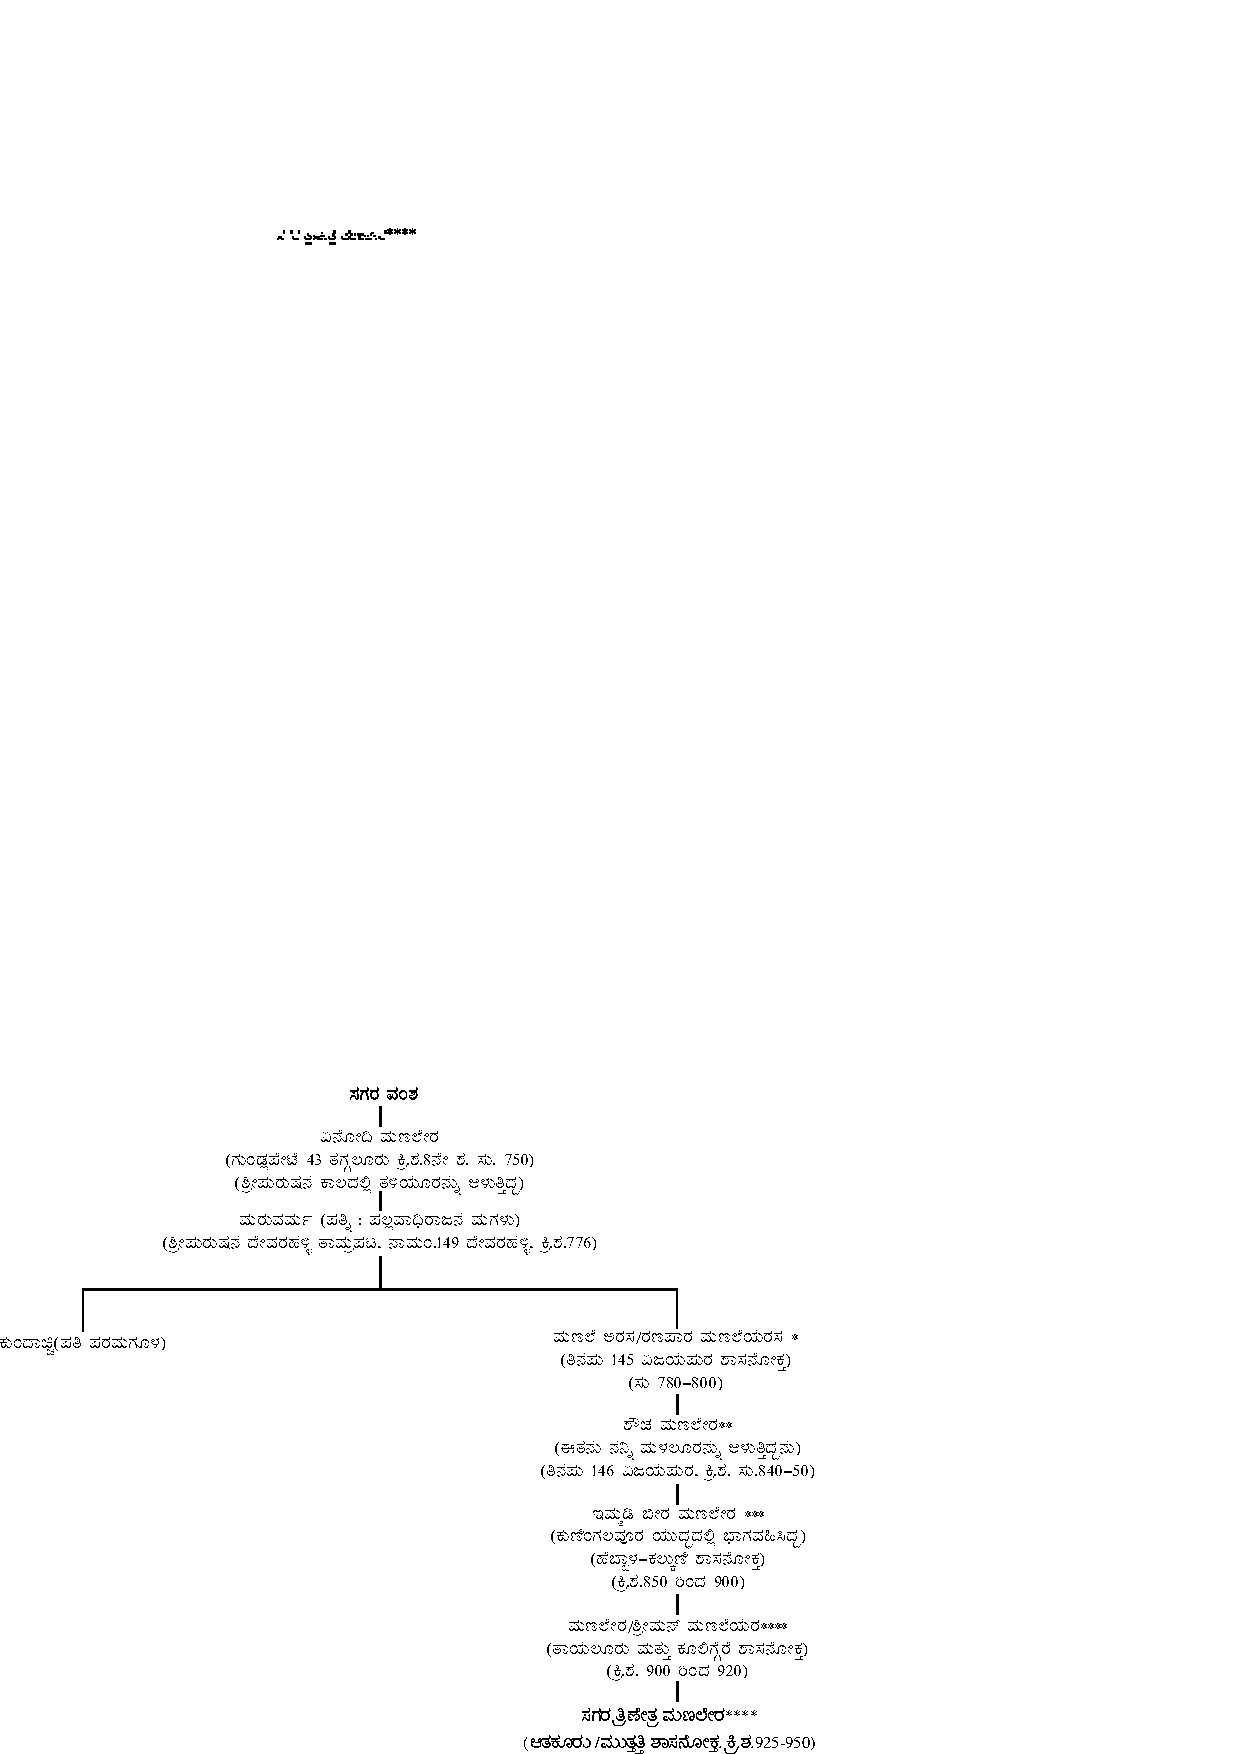
\includegraphics{"images/chap2/1a.jpeg"}
\end{figure}

\textbf{*ಮಣಲೆ ಅರಸ/ ರಣಪಾರ ಮಣಲೆಯರ: } ಕೊಂಗುಣಿ ಮುತ್ತರಸ ಶಿವಮಾರನ ಕಾಲದಲ್ಲಿ ಕೂಂಬಡಿ ಮತ್ತು ಕಿಳಲೆ ನಾಡನ್ನು ಆಳುತ್ತಿದ್ದ ಮಣಲೆ ಅರಸ/ ವಿಜಯಪುರದ ಇನ್ನೊಂದು ಶಾಸನದಲ್ಲಿ ಇವನನ್ನು ರಣಪಾರರ್​ ಮಣಲೆ ಅರಸರ್​ ಎಂದು ಕರೆದಿದೆ. 

**ಶೌಚ ಮಣಲೆಯರ: ಎರೆಯಪ್ಪರಸ ಕಾಲದಲ್ಲಿ ಶೌಚ ನನ್ನಿ ಮಳಲೂರನ್ನು ಆಳುತ್ತಿದ್ದಾಗ, ರಣಪಾರ ಮಣಲೆ ಅರಸರ ಸಮಾಧಿಯ ನಿರ್ವಹಣೆಗೆ ದತ್ತಿಯನ್ನು ಬಿಡಿಸಿದ.

***ಇಮ್ಮಡಿ ಬೀರ ಮಣಲೆಯರ: ಒಂದನೇ ಬೂತುಗನ ರಾಣಿ ಪರಮಬ್ಬೆ ಕುಣಿಗಲ್​ ನಾಡನ್ನು ಆಳುತ್ತಿದ್ದಳು. ಒಂದನೇ ಬೂತುಗ ಮತ್ತು ಅವನ ಮಗ ಎರೆಯಪ್ಪನ ಕಾಲದಲ್ಲಿ ನೊಳಂಬರು, ರಾಷ್ಟ್ರಕೂಟರು ಗಂಗವಾಡಿಯ ಮೇಲೆ ಮಣ್ಣೆ ಮತ್ತು ಕುಣಿಗಲ್​ ಕಡೆಯಿಂದ ದಾಳಿ ಮಾಡಿದರು. ತಾಯಲೂರು ಶಾಸನದ ಕಾಲ ಕ್ರಿ.ಶ.895\enginline{–}96 ಆಗಿದ್ದು ಇದೇ ಕಾಲವು ಇಮ್ಮಡಿ ಬೀರ ಮಣಲೇರನ ಕಾಲವಾಗಿದೆ. ನೊಳಂಬರೊಡನೆ ನಡೆಸಿದ ಯುದ್ಧದಲ್ಲಿ ಇವನು ಮರಣ ಹೊಂದಿರುವ ಸಾಧ್ಯತೆ ಇದೆ. 

\newpage

**** ಶ‍್ರೀಮನ್​ ಮಣಲೆಯರ: ಕನಕಗಿರಿ ತೀರ್ಥದ ಮೇಲೆ ಬಸದಿಯನ್ನು ನಿರ್ಮಿಸಿದ. ತಾಯಲೂರು ಮತ್ತು ಕೂಲಿಗ್ಗೆರೆ ಶಾಸನೋಕ್ತ ಎರೆಯಪ್ಪನ ಕಾಲ ಸು. ಕ್ರಿ.ಶ.907\enginline{–}920) 

***** ಸಗರ ತ್ರಿಣೇತ್ರ, ವಳಭೀಪುರೇಶ್ವರ, ಕದನೈಕ ಸೂದ್ರಕ: ಗಂಗ ಇಮ್ಮಡಿ ಬೂತುಗನ ಜೊತೆ ತಕ್ಕೋಲಂ ಯುದ್ಧದಲ್ಲಿ ಭಾಗವಹಿಸಿ ಹೋರಾಡಿ, ಆತಕೂರು 12ನ್ನು, ಬೆಳ್ವೊಲನಾಡಿನ ಕಾಡಿಯೂರನ್ನು (ಕಳಸ) ಮೆಚ್ಚುಗೆಯಾಗಿ ಪಡೆದನು.


\section{ಚೋಳರು}

ಕರ್ನಾಟಕವನ್ನು ಆಳುತ್ತಿದ್ದ ರಾಜಮನೆತನಗಳಿಗೂ, ತಮಿಳುನಾಡನ್ನು ಆಳುತ್ತಿದ್ದ ರಾಜಮನೆತನಗಳಿಗೂ ಮೊದಲಿನಿಂದಲೂ ರಾಜಕೀಯ ತಿಕ್ಕಾಟ ಇದ್ದುದು ಇತಿಹಾಸದಿಂದ ತಿಳಿದುಬರುತ್ತದೆ. ಅನೇಕವೇಳೆ ವೈವಾಹಿಕ ಸಂಬಂಧ ಇದ್ದರೂ ಅದನ್ನು ಲೆಕ್ಕಿಸದೆ ರಾಜಕೀಯ ಮೇಲ್ಮೆಯನ್ನೇ ಪ್ರತಿಷ್ಠೆಯಾಗಿ ತೆಗೆದುಕೊಂಡು ಕಾದಾಡಿದ್ದಾರೆ. ಮೊಲಿಗೆ ಹೆಚ್ಚಾಗಿ ಕರ್ನಾಟಕದ ರಾಜಮನೆತನಗಳು ಮೇಲುಗೈ ಸಾಧಿಸಿವೆ. ಆದರೆ ಗಂಗರ ಕೊನೆಗಾಲದಲ್ಲಿ ಚೋಳರು ಮೇಲುಗೈ ಸಾಧಿಸಿ, ಗಂಗವಾಡಿಯನ್ನು ಆಕ್ರಮಿಸಿಕೊಂಡರು.

ಗಂಗರ ಕೊನೆಯ ಅರಸರನ್ನು, ಅವರ ಅಧಿನರಾಗಿ ಆಗತಾನೆ ತಲೆ ಎತ್ತುತ್ತಿದ್ದ ಹೊಯ್ಸಳರನ್ನು, ಸುಮಾರು ಕ್ರಿ.ಶ.1004 ರಲ್ಲಿ ಪೂರ್ಣವಾಗಿ ಸೋಲಿಸಿ ಸುಮಾರು 112 ವರ್ಷಗಳ ಕಾಲ ಅಂದರೆ, ಕ್ರಿ.ಶ.1116ರವರೆಗೆ ಗಂಗವಾಡಿಯನ್ನು ಆಳಿದರು ಎಂದು ರೈಸ್​ರವರು ಹೇಳಿದ್ದಾರೆ.\endnote{ \engfoot{Rice, B.L., Mysore and Coorg from the Inscriptions, pp.82,83}} ಕಲಿಯೂರಿನ ಅಪ್ರಮೇಯ ದಂಡನಾಯಕನ ಶಾಸನವನ್ನು ನೋಡಿದರೆ, ಚೋಳರು ಕೊಳ್ಳೇಗಾಲದ ಕಡೆಯಿಂದ ಗಂಗರ ರಾಜಧಾನಿ ತಲಕಾಡನ್ನು ಹಿಡಿದ ಹಾಗೆ ತೋರುತ್ತದೆ. 

ಕಲವೂರ ಕಾಳಗದಲ್ಲಿ ಚೋಳರೊಡನೆ ನಡೆದ ಭಾರೀ ಯುದ್ಧದಲ್ಲಿ ಭಾಗವಹಿಸಿ, ಮರಣಹೊಂದಿದವರ ಹಾಗೂ ಸೋತವರ ಪಟ್ಟಿಯನ್ನು ಅಪ್ರಮೇಯ ದಂಡನಾಯಕನ ಕಲಿಯೂರು ಶಾಸನ ನೀಡಿದೆ.\endnote{ ಎಕ 5 ತಿ.ನರಸಿಪುರ 220 ಕಲಿಯೂರು 1006} ಮಲೆಪರಮಲ್ಲ, ಚೊತ್ತರಳಿ, ಗೋಯಿಗ, ಬೂತುಗ, ಸೇನವಾರ, ಪೊಯ್ಸಳ, ಬೆಳ್ಗುಪ್ಪ, ಜೊರೆಗ, ಸಂಚಿಗ, ಕಕ್ಕಗ, ಸಿನ್ನಿವರ, ಮಾಗಲ, ಯೆರೆಗಂಗ, ಮರ್ದ್ದಸ, ಬರಮಣ್ಣ, ಮೊದಲಾದವರು ಸತ್ತರೆಂದು, ಗಂಡರಗಂಡಮುಂಡ ಜಗಕಾರಿಗ ಬೀರುಗ, ನಾಗಮರ್ವ, ಮಾಗುಂಡರಕಿಲ್ಲ, ಮತ್ತಯರ, ನೊಳಂಬರ ಚಂದಿಗ, ಪೊನ್ನ, ನನ್ನಿಗ, ಮಂಡರಿವರ್ಮರಾಜ, ನರಗ, ಸಿರಿಗ, ಎಳಗ ಪೊಯ್ಸಳನೆಂಬ ಅನಂತ ಬಲರನ್ನು, ಅಪ್ರಮೇಯನು ಕಲಿಯೂರು ಯುದ್ಧರಂಗದಲ್ಲಿ ಸೋಲಿಸಿ ಓಡಿಸಿದನೆಂದೂ ಕಲಿಯೂರು ಶಾಸನದಲ್ಲಿ ಹೇಳಿದೆ. ಇವರಲ್ಲಿ ಸತ್ತವರ ಪೈಕಿ ಮಲೆಪರಮಲ್ಲ, ಪೊಯ್ಸಳ, ಇವರು ಹೊಯ್ಸಳ ವಂಶದವರೆಂದು, ಗೋಯಿಗ, ಬೂತುಗ, ಎರೆಗಂಗ ಗಂಗವಂಶದರೆಂದೂ ಹೇಳಬಹುದು. ಸೋತು ಉಳಿದವರಲ್ಲಿ ಎಳಗನೆಂಬ ಪೊಯ್ಸಳನು ಹೊಯ್ಸಳ ವಂಶದವನು. ಚೋಳರ ಕೈಕೆಳಗೆ ಗಂಗಪೆರ್ಮಾನಡಿಯು ಕುಂದೂರು ನಾಡನ್ನು ಆಳುತ್ತಿದ್ದನೆಂದು ಹೇಳಿದೆ.\endnote{ ಎಕ 7 ಮಂ 67 ಬೇಲೂರು 997} ಕ್ರಿ.ಶ.986ರಲ್ಲಿ ನಾಲ್ಕನೇ ರಾಚಮಲ್ಲನ ತಮ್ಮ ಐದನೇ ರಾಚಮಲ್ಲ ರಕ್ಕಸಗಂಗನು ಪಟ್ಟಕ್ಕೆ ಬಂದನು. ಕ್ರಿ.ಶ.999 ರಲ್ಲಿ ಚೋಳರು ಗಂಗವಾಡಿಯನ್ನು ಗೆದ್ದುಕೊಂಡರು. ಇದೇ ವರ್ಷ ನೀತಿಮಾರ್ಗ ಪೆರ್ಮಾನಡಿಯೆಂಬ ಒಬ್ಬ ಗಂಗ ಅರಸನು ಶಾಸನೋಕ್ತನಾಗಿದ್ದು, ಇವನಿಗೂ ಹಿಂದಣ ಗಂಗ ಅರಸರಿಗೂ ಸಂಬಂಧವೇನೆಂದು ತಿಳಿಯದು ಎಂದು ಇತಿಹಾಸ ವಿದ್ವಾಂಸರು ಹೇಳಿದ್ದಾರೆ.\endnote{ ಸೂರ್ಯನಾಥಕಾಮತ್​ ಡಾ॥, ಕರ್ನಾಟಕದ ಸಂಕ್ಷಿಪ್ತ ಇತಿಹಾಸ, ಪುಟ 38} ಆದುದರಿಂದ ಚೋಳರು ಗಂಗವಾಡಿಯನ್ನು ಆಕ್ರಮಿಸಿದಮೇಲೂ, ರಕ್ಕಸಗಂಗನು ಕುಂದೂರು ನಾಡನ್ನು ಆಳುತ್ತಿದ್ದನೆಂದು ಹೇಳಬಹುದು. ಈ ಹಿನ್ನೆಲೆಯಲ್ಲಿ ಮಂಡ್ಯ ಜಿಲ್ಲೆಯಲ್ಲಿ ಚೋಳರ ಇತಿಹಾಸವನ್ನು ಗುರುತಿಸಬಹುದು.

ಶ‍್ರೀ ರಾಜರಾಜದೇವನ ಕಾಲದಲ್ಲಿ ಕಣ್ಣನೆಂಬುವವನು ಚಿಕವಂಗಲವಕ್ಕೆ ಮುತ್ತಿಗೆ ಹಾಕಿ ತುರುಗಳನ್ನು ಹಿಡಿದಾಗ, ಬಂಗಲಿ ಎರೆಯಮ್ಮನ ಮಗ ನಾಗಯ್ಯ ಎಂಬುವವನು ಕಾದಿ ಮಡಿದನೆಂದು ಚಿನಕುರಳಿ ವೀರಗಲ್ಲು ಶಾಸನದಿಂದ ತಿಳಿದುಬರುತ್ತದೆ.\endnote{ ಎಕ 6 ಪಾಂಪು 50 ಚಿನಕುರಳಿ 1011} ಶಾಸನೋಕ್ತ ರಾಜರಾಜದೇವನು ಒಂದನೆಯ ರಾಜರಾಜಚೋಳನೆಂದು ಗುರುತಿಸಬಹುದು. ಒಂದನೇ ರಾಜರಾಜ ಚೋಳನ ಮಗ, ಪ್ರಚಂಡ ದಂಡನಾಯಕ ಪಂಚವನ್​ ಮಹಾರಾಯನ ಬಲಮುರಿ ಶಾಸನವೇ ಮಂಡ್ಯ ಜಿಲ್ಲೆಯಲ್ಲಿ ದೊರಕುವ ಚೋಳರ ಅತ್ಯಂತ ಪ್ರಮುಖವಾದ ಮೊದಲನೆಯ ಶಾಸನ. ರಾಜರಾಜಚೋಳನ 28ನೇ ರಾಜ್ಯ ಸಂವತ್ಸರದಲ್ಲಿ ಅಂದರೆ, ಕ್ರಿ.ಶ.1012\enginline{–}13 ರಲ್ಲಿ, ಈ ಶಾಸನವನ್ನು ಹಾಕಿಸಲಾಗಿದೆ.\endnote{ ಎಕ 6 ಶ‍್ರೀಪ 78 ಬಲಮುರಿ 1012–13} ಈತನನ್ನು ಗಂಗವಾಡಿಯ ಮಹಾಮಂಡಲೇಶ್ವರನನ್ನಾಗಿ ನೇಮಿಸಿ ಎಡದೊರೆನಾಡಿಗೆ ಕಳುಹಿಸಲಾಗಿತ್ತು. ಮುಮ್ಮಡಿ ಚೋಳನ ಗಂಧವಾರಣನೆಂದು ಶಾಸನದಲ್ಲಿ ಹೇಳಿರುವುದರಿಂದ ಇವನು ಒಂದನೇ ರಾಜೇಂದ್ರಚೋಳನೇ ಆಗಿದ್ದಾನೆ. ಈ ಪಂಚವನ್​ ಮಹಾರಾಯನು ವೆಂಗಿಮಂಡಲ ಮತ್ತು ಗಂಗಮಂಡಲಗಳಿಗೆ ಮಹಾದಂಡನಾಯಕ ಪದವಿಯನ್ನು ಪಡೆದು ಪ್ರವರ್ತಿಸುತ್ತಿದ್ದನೆಂದು ಈ ಶಾಸನದಲ್ಲಿ ಸ್ಪಷ್ಟವಾಗಿ ಹೇಳಿದೆ. ಇವನು ತುಳುವ, ಕೊಂಕಣ, ಮಲೆ, ಚೇರ, ರಟ್ಟಪಾಡಿ, ಬೆಂಗಿ, ಬೆಳ್ವಲ, ಗಂಗಾವನಿರಟ್ಟವಾಡಿ, ಮಲೆನಾಡೇಳು, ನೊಳಂಬ, ಆಂಧ್ರ, ಕೊಂಗು, ಕಳಿಂಗ, ಪಾಂಡ್ಯ ವಿಷಯಾಧೀಶರನ್ನು ಸೋಲಿಸಿ, ಈ ಪ್ರದೇಶಗಳನ್ನು ಚೋಳನಾಡನ್ನಾಗಿ ಮಾಡಿದನೆಂದು ಈ ಶಾಸನದಲ್ಲಿ ಹೇಳಿದೆ. ಮಲೆನಾಡೇಳು ಅಂದರೆ ಏಳು ಮಲೆನಾಡುಗಳು ಯಾವುವು ಎಂದು ತಿಳಿದುಬರುವುದಿಲ್ಲ. ರಾಜರಾಜಚೋಳನಿಗೆ ಚಕ್ರೇಶ್ವರ, ಶ‍್ರೀಕೋವಿರಾಜ ರಾಜಕೇಸರಿವರ್ಮ, ಎಂಬ ಬಿರುದುಗಳು ಇದ್ದುದು ಈ ಶಾಸನದಿಂದ ತಿಳಿದುಬರುತ್ತದೆ. ಪಂಚವನ್​ ಮಹಾರಾಯನು ‘ಬಳ್ಳೆಗೊಳದ ಬಲಂಬುತೀರ್ಥ’ದಲ್ಲಿ (ಬಲಮುರಿ) ಮಿಂದು, ಮಹಾದೇವರ(ಇಂದಿನ ಅಗಸ್ತ್ಯೇಶ್ವರ) ನೈವೇದ್ಯ\-ಕ್ಕಾಗಿ ಅಲ್ಲಿಯ ಮಹಾಜನರನ್ನು ಕೇಳಿ ದತ್ತಿ ಬಿಟ್ಟನೆಂದು ಬಲಮುರಿ ಶಾಸನದಲ್ಲಿ ಹೇಳಿದೆ. 

ಒಂದನೇ ರಾಜರಾಜಚೋಳನ ಮಗ ರಾಜೇಂದ್ರ ಚೋಳನಿಗೆ ‘ಪಂಚವನ್​ಮಹಾರಾಯ’ನೆಂಬ ಬಿರುದು ಇತ್ತು.\endnote{ ಎಪಿಗ್ರಾಫಿಯಾ ಕರ್ನಾಟಿಕಾ, ಸಂಪುಟ 3, ಪೀಠಿಕೆ, ಪುಟ 73–74} ಕಿರಂಗೂರಿನ ಕೋದಂಡರಾಮ ದೇವಾಲಯದ ತಳಪಾದಿಯ ಕಲ್ಲಿನ ಮೇಲಿರುವ ಶಾಸನದಲ್ಲಿ “ತನಂಗಾಡಿಯಾದ\break ಪಂಚವಮಾರಾಯನಾದ ರಾಜೇನ್ದ್ರಚೋೞ ವೞ್ದರೆಯನ್ಯಮ್ಮೂರೊಳೆ ಮಾಡಿಸಿದ” ಎಂದು ಹೇಳಿದೆ. ಈ ‘ವೞ್ದರೆ’ ಎಂದರೇನು ಎಂದು ತಿಳಿದುಬರುವುದಿಲ್ಲ. ತನಂಗಾಡಿ ಎಂಬುದೂ ಕೂಡಾ ಅವನ ಬಿರುದೇ ಅಥವಾ ಅದಕ್ಕೆ ಬೇರೆ ಅರ್ಥವಿದೆಯೇ ಗೊತ್ತಾಗುವುದಿಲ್ಲ. ಮೂಲತಃ ಇದು ರಾಮದೇವರ ದೇವಾಲಯವೇ ಆಗಿದ್ದಲ್ಲಿ, ಚೋಳರು ಶೈವ ಪಕ್ಷಪಾತಿಗಳಾಗಿದ್ದರೂ ಕೂಡಾ, ವೈಷ್ಣವ ವಿರೋಧಿಗಳಾಗಿರಲಿಲ್ಲ ಎಂದು ಹೇಳಬಹುದು.

ಒಂದನೇ ರಾಜರಾಜಚೋಳನ ನಂತರ ಪಟ್ಟಕ್ಕೆ ಬಂದ ಅವನ ಮಗ ಒಂದನೇ ರಾಜೇಂದ್ರ ಚೋಳನ ದಿಗ್ವಿಜಯಗಳನ್ನು ವರ್ಣಿಸುವ ಪ್ರಶಸ್ತಿ ಶಾಸನ ಹಳೇಬೂದನೂರಿನಲ್ಲಿದೆ. ಇದು ಅವನ 13ನೇ ಆಡಳಿತ ವರ್ಷದಲ್ಲಿ ಅಂದರೆ ಕ್ರಿ.ಶ. 1024ರಲ್ಲಿ ಹೊರಟಿದೆ. ಎಡದೊರೆನಾಡು, ವನವೇಲಿ, ವನವಾಸಿ, ಕೊಳ್ಳಿಪಾಕೆ, ಚೇರ, ರಟ್ಟಪಾಡಿ ಏಳರಲಕ್ಕ(ಏಳೂವರೆಲಕ್ಷ), ಏಳುಮಲೆ, ಚಕ್ರಗೊಟ್ಟ, ಮುದಿಮಲೆ, ಮಧುರಮಂಡಲ, ವೆಂಜಿಮಲೈ ಅಥವಾ ಪ್ರಾಚೀನ ಮಸುನಿದೇಶ, ಪಂಚಂಪಲ್ಲಿ ಮುಂತಾದ ದೇಶಗಳನ್ನು ವಶಪಡಿಸಿಕೊಂಡ ವಿಚಾರ ಈ ಶಾಸನದಲ್ಲಿದೆ. ಕಲ್ಯಾಣದ ಚಾಲುಕ್ಯರ ಜಯಸಿಂಹನನ್ನು ಸೋಲಿಸಿ, ರಟ್ಟಪಾಡಿ ಏಳೂವರೆಲಕ್ಷವನ್ನು ವಶಪಡಿಸಿಕೊಂಡಿದ್ದನ್ನು, ಅವನು ನವನಿಧಿಕುಲಪರ್ವತದ ಹಿಂದೆ ಅಡಗಿದ್ದನ್ನು ಹಳೇಬೂದನೂರು ಶಾಸನದಲ್ಲಿ ಹೇಳಿದೆ.\endnote{ ಎಕ 7 ಮಂ 53 ಹಳೇಬೂದನೂರು 1024}

ರಾಜೇಂದ್ರ ಚೋಳನು ಆನೆಗಳ ಸೇನೆಯ ಮೂಲಕ ಶತ್ರುರಾಜರುಗಳಿಗೆ ಭಯಂಕರನಾಗಿ, ಅವರ ಹೆಂಡಿರನ್ನು ಭಂಡಾರವನ್ನು ವಶಪಡಿಸಿಕೊಂಡದ್ದು, ಗಂಗಾನದಿ ಬಯಲಿನವರೆಗೂ ತನ್ನ ದಂಡಯಾತ್ರೆಯನ್ನು ನಡೆಸಿದ್ದು, ನೌಕಾಸೇನೆಯ ಮೂಲಕ ಮಲಯ ಪರ್ಯಾಯ ದ್ವೀಪವನ್ನು ಆಕ್ರಮಿಸಿ, ಶ‍್ರೀವಿಜಯ ಸಾಮ್ರಾಜ್ಯವನ್ನು ನಾಶಮಾಡಿ, ಅಲ್ಲಿಯ ರಾಜ ವಿಜಯೋತ್ತುಂಗ ವರ್ಮನನ್ನು ಸೋಲಿಸಿ, ಅವನ ರಾಜಧಾನಿ ಕಡಾರಂನ್ನು ಆಕ್ರಮಿಸಿದ್ದು, ಇವನು ನೂತನವಾಗಿ ನಿರ್ಮಿಸಿದ ರಾಜಧಾನಿ ಗಂಗೈಕೊಂಡಚೋಳಪುರಕ್ಕೆ ವಿದ್ಯಾಧರ ತೋರಣವನ್ನು ನಿರ್ಮಿಸಿದ ವಿಷಯಗಳು, ವೈದ್ಯನಾಥಪುರ ತಮಿಳು ತ್ರುಟಿತ ಶಾಸನ\-ದಲ್ಲಿದೆ.\endnote{ ಎಕ 7 ಮ 72 ವೈದ್ಯನಾಥಪುರ 11ನೇ ಶ.} ಬಹುಶಃ ಇದೇ ಅರಸನು ಅರ್ಕೇಶ್ವರನ ತಿರುನಂದಾದೀಪಕ್ಕೆ ದತ್ತಿ ನೀಡಿರುವ ಸೂಚನೆ ಇದೇ ಕಾಲದ ತ್ರುಟಿತವಾಗಿರುವ ಗುತ್ತಲು ಶಾಸನದಲ್ಲಿದೆ.\endnote{ ಎಕ 7 ಮಂ 64 ಗುತ್ತಲು 11ನೇ ಶ.} ಗಂಗಾನದಿಯ ಪ್ರಸ್ತಾಪವಿರುವ ರಾಜೇಂದ್ರಚೋಳನ ಶಾಸನದ ಚನ್ನಪ್ಪನದೊಡ್ಡಿಯಲ್ಲಿದೆ.\endnote{ ಎಕ 7 ಮಂ 65 ಚನ್ನಪ್ಪನದೊಡ್ಡಿ 11ನೇ ಶ.} ರಾಜೇಂದ್ರ ಚೋಳನು ತನ್ನ ವಿಜಯಗಳ ಸ್ಮರಣಾರ್ಥ ಗಂಗೈಕೊಂಡ ಚೋಳಪುರದ ಬಳಿ ದೊಡ್ಡದೊಂದು ಕೆರೆಯನ್ನು ನಿರ್ಮಿಸಿ ಗಂಗಾನದಿಯ ಬಯಲಿನ ಅರಸರನ್ನು ಗೆದ್ದಾಗ ಅಲ್ಲಿಂದ ತಂದಿದ್ದ ಪವಿತ್ರಜಲವನ್ನು ಆ ಕೆರೆಯಲ್ಲಿ ಸುರಿದ ವಿಚಾರ ನಮಗೆ ಇತಿಹಾಸದಿಂದ ತಿಳಿದುಬರುತ್ತದೆ. ಉತ್ತಮಚೋಳ, ಪರಕೇಸರಿ ಎಂಬ ಬಿರುದುಗಳು ಮಾತ್ರ ಕಂಡುಬರುವ ಸಂಪೂರ್ಣ ತ್ರುಟಿತ ಶಾಸನವೂ ಚನ್ನಪ್ಪನದೊಡ್ಡಿಯಲ್ಲಿದೆ.\endnote{ ಎಕ 7 ಮಂ 66 ಚನ್ನಪ್ಪನದೊಡ್ಡಿ 11ನೇ ಶ.} ಇವು ಒಂದನೇ ರಾಜೇಂದ್ರಚೋಳನ ಬಿರುದುಗಳು. 

ಮುಂದೆ ಪಟ್ಟಕ್ಕೆ ಬಂದ ವೀರರಾಜೇಂದ್ರನ ಸೋದರಳಿಯನಾದ ಕುಲೋತ್ತುಂಗ ಚೋಳನ (1070\enginline{–}1120)ಮೂರು ಶಾಸನಗಳು ಜಿಲ್ಲೆಯಲ್ಲಿ ದೊರಕಿದ್ದು ಅವು ತಮಿಳು ಭಾಷೆ ಮತ್ತು ಗ್ರಂಥ ಲಿಪಿಯಲ್ಲಿವೆ. ಈತನ 22ನೇ ರಾಜ್ಯಸಂವತ್ಸರದಲ್ಲಿ ಅವನ ಮಾಂಡಲಿಕನಾಗಿ ಇಡೈತುರೈನಾಡನ್ನು (ಎಡದೊರೆನಾಡು) ಆಳುತ್ತಿದ್ದ, ವಿರುದಯರಾಯ ಭಯಂಕರ ಮಾರಾಯನ್​ ಪೋಮನ್​ ಇರಾಮನ್​ ಎಂಬುವವನು ಸಿರಿಯಕಲಸತ್ತುಪಾಡಿಯಾದ (ಇಂದಿನ ಕಲಸ್ತವಾಡಿ) ವಾನವನ್​ಮಾದೇವಿ ಚತುರ್ವೇದಿ ಮಂಗಲಮ್ ಎಂಬ ಅಗ್ರಹಾರದಲ್ಲಿ 200 ವರ್ಷಗಳಿಂದ ಹಾಳಾಗಿದ್ದ ಕೆರೆಯನ್ನು ಜೀರ್ಣೋದ್ಧಾರ ಮಾಡಿದನು.\endnote{ ಎಕ 6 ಶ‍್ರೀಪ 67 ಬೊಮ್ಮೂರು ಅಗ್ರಹಾರ 1102–03} ವಾನವನ್​ ಮಹಾದೇವಿಯು ಒಂದನೇ ರಾಜರಾಜಚೋಳನ ತಾಯಿ. ಈತನ ಕಾಲದಲ್ಲಿ ಕಾಂಚಿಗೊಂಡ ಪಲ್ಲವರಾಯ ರಾಜವಿದ್ಯಾಧರ ಅಯಿರಮೆನಾಯಕ ಅರಿಕುಂಟೆ ದಮ್ಮಿಸೆಟ್ಟಿಯರ ಮಗ, ಒಡೆಯನಂಬಿಯಾದ ಉದಯಾದಿತ್ಯ ಪಲ್ಲವರಾಯನೆಂಬ ವ್ಯಾಪಾರಿಯು ಕಟ್ಟಿಸಿದ ಕೆರೆಗೆ ಹೊಳಲಯನಾಡ ತೊಲಗದ ಗಂಡ ಅರಕೆರೆ ನಾಡಾಳುವ ಬೀರಗವುಂಡನು ಭೂಮಿಯನ್ನು ಬಿಡುತ್ತಾನೆ.\endnote{ ಎಕ 6 ಶ‍್ರೀಪ 113 ಅರಕೆರೆ 1108} ಈತನ 45ನೇ ರಾಜ್ಯಸಂವತ್ಸರದಲ್ಲಿ ವಡುಗವೇಳೆಕಾರ ಮುತಹಡೆಯರಾಯನ ಮಕ್ಕಳು ಮಾದಿಯಣ್ಣ, ಲಕ್ಕಣ್ಣ ಇವರು ಎರಡು ದೇವಾಲಯಗಳನ್ನು ನಿರ್ಮಿಸಿ ಅದಕ್ಕೆ ಭೂಮಿಯನ್ನು ಬಿಟ್ಟರೆಂದು ಹೇಳಿದೆ.\endnote{ ಎಕ 6 ಪಾಂಪು 44 ಕನ್ನಂಬಾಡಿ 1114–15} ಈ ಶಾಸನದ ಕೆಳಭಾಗದಲ್ಲಿಯೇ ಇನ್ನೊಂದು ಶಾಸನವಿದ್ದು ಅದರಲ್ಲಿ ಉದಯಾದಿತ್ಯ ಪಲ್ಲವರಾಯನನ್ನು ಮಲೆಯಾಳ ಪಡೆಗಳಿಗೆ ಮುಖ್ಯಸ್ಥನೆಂದು ಹೇಳಿದೆ.\endnote{ ಎಕ 6 ಪಾಂಪು 45 ಕನ್ನಂಬಾಡಿ 12ನೇ ಶ.} ಹಾಗೂ ಕುಲೋತ್ತುಂಗ ಚೋಳ ಪಲ್ಲವರಾಯ, ಇರುಮುಡಿಚೋಳ ಪಲ್ಲವರಾಯ, ರಾಜಕುಂಜರ ಪಲ್ಲವರಾಯ, ಪಡೈಕ್ಕಣಕ್ಕನ್​ ಮಲೆಯಾಂಡನ್​ ಇವರುಗಳನ್ನು ಉಲ್ಲೇಖಿಸಿದೆ. ಇವರೆಲ್ಲರೂ ಸೇನಾಪಡೆಯ ಅಧಿಕಾರಿಗಳಿರಬಹುದು.


\section{ಹೊಯ್ಸಳರು}

ಇಂದಿನ ಮಂಡ್ಯಜಿಲ್ಲೆಯು ಹೊಯ್ಸಳ ಸಾಮ್ರಾಜ್ಯದ ಅಥವಾ ಗಂಗವಾಡಿ ತೊಂಬತ್ತಾರುಸಾವಿರದ ಆಯಕಟ್ಟಿನ ಪ್ರದೇಶದಲ್ಲಿತ್ತು. ಜಿಲ್ಲೆಯ ದಕ್ಷಿಣಕ್ಕೆ ಕಾವೇರಿ ನದಿಯಾಚೆ ಚೋಳರಿಂದ ಆಕ್ರಮಿತವಾಗಿ ಹೊಯ್ಸಳರ ವಶಕ್ಕೆ ಬಂದು ಹೊಯ್ಸಳಸಾಮ್ರಾಜ್ಯ ಸ್ಥಾಪನೆಗೆ ಮೂಲವಾದ ತಲಕಾಡು, ಪಶ್ಚಿಮಕ್ಕೆ ಕೊಂಗಾಳ್ವರ ರಾಜ್ಯ, ಉತ್ತರಕ್ಕೆ ಹೊಯ್ಸಳರ ರಾಜಧಾನಿಗಳಾದ ದೋರಸಮುದ್ರ\break (ಹಳೆಯಬೀಡು) ಮತ್ತು ಬೇಲೂರು, ಪೂರ್ವಕ್ಕೆ ಮಾಗಡಿ ಸೀಮೆಯ ಪ್ರದೇಶ, ಇವುಗಳ ಮಧ್ಯದಲ್ಲಿ ಮಂಡ್ಯಜಿಲ್ಲೆಯಲ್ಲಿ ಹೊಯ್ಸಳರ ನೆಲೆಬೀಡುಗಳೂ, ಧಾರ್ಮಿಕ ಹಾಗೂ ಆರ್ಥಿಕ ಕೇಂದ್ರಗಳೂ ಆದ \textbf{ಮದ್ದೂರು, ತೊಣ್ಣೂರು, ಕೋಡಾಲ, ಮೇಲುಕೋಟೆ, ನಾಗಮಂಗಲ, ಬಸರಾಳು, ಬೆಳ್ಳೂರು, ದಡಿಗ, ಕಿಕ್ಕೇರಿ, ಹೊಸಹೊಳಲು, ತೊಳಸಿ, ಮಾಳಗೂರು}, ಮುಂತಾದ ಊರುಗಳು ಇವೆ. \textbf{ಮಂಡ್ಯ ಜಿಲ್ಲೆಯಲ್ಲಿ ಹೊಯ್ಸಳರಿಗೆ ಸೇರಿದ ಸುಮಾರು 243 ಶಾಸನಗಳು, ಸುಮಾರು 26 ಪ್ರಮುಖ ಹೊಯ್ಸಳರ ದೇವಾಲಯಗಳೂ ಇರುವುದು, ಹೊಯ್ಸಳರು ಈ ಪ್ರದೇಶಕ್ಕೆ ಎಷ್ಟೊಂದು ಮಹತ್ವ ನೀಡಿದ್ದರು ಎಂಬುದನ್ನು ತೋರಿಸುತ್ತಿದೆ}.

\textbf{ಹೊಯ್ಸಳ ವಂಶದ ಮೂಲಕಥೆ: } ಹೊಯ್ಸಳ ವಂಶದ ಉಗಮದ ಪಾರಂಪರಿಕ ಕಥೆಯನ್ನುಹೇಳುವ ಹಾಗೂ ಅವರ ವಂಶಾವಳಿಯ ವಿವರವನ್ನು ನೀಡುವ ಅನೇಕ ಶಾಸನಗಳು ಜಿಲ್ಲೆಯಲ್ಲಿ ದೊರಕಿವೆ. ಈ ಶಾಸನಗಳಲ್ಲಿ ಬರುವ ಹೊಯ್ಸಳ ವಂಶದ ಮೂಲಕಥೆಯು ಸಾಮಾನ್ಯವಾಗಿ ಈ ರೀತಿ ಇದೆ. ಶಶಕಪುರದ ವಾಸಂತಿಕಾ ದೇವಾಲಯದಲ್ಲಿ ಮುನಿಯೊಬ್ಬನು ಸಳನಿಗೆ ವಿದ್ಯಾಭ್ಯಾಸ ಮಾಡಿಸುತ್ತಿದ್ದಾಗ ಇದ್ದಕ್ಕಿದ್ದ ಹಾಗೆ ಅಲ್ಲಿಗೆ ಹುಲಿಯೊಂದು ಬಂದಿತು. ಆ ಮುನೀಂದ್ರನು ಸಳನಿಗೆ ಸಲಾಕೆಯೊಂದನ್ನು ಕೊಟ್ಟು ಪೊಯ್​ ಸಳ (ಹೊಯ್​ ಸಳ) ಎಂದು ಹೇಳಿದನು. ಸಳನು ಆ ಸಲಾಕೆಯಿಂದಲೇ ಹುಲಿಯನ್ನು ಕೊಂದನು. ಅಂದಿನಿಂದ ಅವನ ವಂಶದವರಿಗೆ ಹೊಯ್ಸಳರೆಂದು ಹೆಸರಾಯಿತು, ಅವರ ರಾಜ್ಯಚಿಹ್ನೆಯೂ ಅದೇ ಆಯಿತು.\endnote{ ಎಕ 7 ನಾಮಂ 74 ಬೆಳ್ಳೂರು 1271, 73 ಬೆಳ್ಳೂರು 1309, 76 ಬೆಳ್ಳೂರು 1309} ಇನ್ನು ಕೆಲವು ಶಾಸನಗಳಲ್ಲಿ ಮುನಿಯ ಆದೇಶದಂತೆ ಸಳನು ಹುಲಿಯನ್ನು ಕೊಂದ ಕಥೆ ಇದೆ. ಆದರೆ ವಾಸಂತಿಕಾ ದೇವಾಲಯದ ಪ್ರಸ್ತಾಪ ಇಲ್ಲ.\endnote{ ಎಕ 7 ನಾಮಂ 118 ಹಟ್ಟಣ 1178, ಎಕ 6 ಕೃಪೇ 82, 83 ಮತ್ತು 84 ಅಗರಹಾರಬಾಚಹಳ್ಳಿ 13ನೇ ಶ.} ಬೆಳ್ಳೂರು ಶಾಸನ ಈ ಮುನಿಯನ್ನು ‘ಜಿನಮುನಿ’ ಎಂದು ಹೇಳುತ್ತದೆ.\endnote{ ಎಕ 7 ನಾಮಂ 81 ಬೆಳ್ಳೂರು 1224} ಲಾಳನಕೆರೆ ಶಾಸನದಲ್ಲಿ ಈ ಕಥೆ ಇಲ್ಲ, ಸಳನು ಜಿನಮುನಿಯಲ್ಲಿ ಅತಿಶಯವಾದ ಭಕ್ತಿಯುಳ್ಳವನಾಗಿದ್ದನೆಂದು ಮಾತ್ರ ಹೇಳಿದೆ.\endnote{ ಎಕ 7 ನಾಮಂ 62 ಲಾಳನಕೆರೆ 1218} ದಡಗ ಶಾಸನದಲ್ಲಿ ಮುನಿಯ ಪ್ರಸ್ತಾಪವಿಲ್ಲ, ಸಳನು ಹುಲಿಯನ್ನು ಕೊಂದನೆಂದು ಮಾತ್ರ ಹೇಳಿದೆ.\endnote{ ಎಕ 7 ನಾಮಂ 68 ದಡಗ, 11ನೇ ಶ.} ಭೀಮನಹಳ್ಳಿ ಶಾಸನವು ಮುನಿಯನ್ನು ‘ದಿವ್ಯಮುನಿವರ’ನೆಂದು ಹೇಳಿದೆ.\endnote{ ಎಕ 7 ನಾಮಂ 173 ಭೀಮನಹಳ್ಳಿ 13ನೇ ಶ.} ಗೋವಿಂದನಹಳ್ಳಿ ಶಾಸನದಲ್ಲಿ ಈ ಕಥೆ ಸ್ವಲ್ಪ ವಿಭಿನ್ನವಾಗಿದೆ.\endnote{ ಎಕ 6 ಕೃಪೇ 39 ಗೋವಿಂದನಹಳ್ಳಿ 1236} ತನ್ನ ಪೂರ್ವಜರು ಆರಾಧಿಸುತ್ತಿದ್ದ ಹಾಗೂ ಶಶಪುರದ ಸಮೀಪದ ಕಾಡಿನಲ್ಲಿದ್ದ, ವಾಸಂತಿಕಾ ದೇವಿಯ ದೇವಾಲಯಕ್ಕೆ ಸಳನು ದರ್ಶನಾರ್ಥವಾಗಿ ಹೋಗಿದ್ದನು. ಅಲ್ಲಿ ಒಬ್ಬ ಮುನಿಯನ್ನು ಕಂಡನು. ಕೆಲವು ಕಾಲ ಅಲ್ಲಿದ್ದು ವೀತಾಯುಧವ್ರತಧಾರಿಯಾಗಿ ಅಂದರೆ, ಆಯುಧಗಳನ್ನು ಹಿಡಿಯದೇ ಇರುವ ವ್ರತವನ್ನು ಕೈಗೊಂಡು ದೇವಿಯನ್ನು ಆರಾಧಿಸಿ ಮುನಿಯನ್ನು ಸತ್ಕರಿಸುತ್ತಿದ್ದಾಗ, ಭೀಕರವಾದ ಹುಲಿಯೊಂದು ಘರ್ಜಿಸುತ್ತಾ ಅಲ್ಲಿಗೆ ಬಂದಿತು. ಆ ಮುನಿಯು ಸಳನಿಗೆ ಸಲಾಕೆಯನ್ನು ನೀಡಿ ಪೊಯ್ಸಳ ಎಂದು ಅದನ್ನು ಎದುರಿಸುವಂತೆ ತಿಳಿಸಿದನು. ಸಳನು ಸಲಾಕೆಯಿಂದ ಹುಲಿಯನ್ನು ಕೊಂದನು. ಮುಂದೆ ಅವನ ವಂಶದವರಿಗೆ ಹೊಯ್ಸಳರೆಂದು ಹೆಸರಾಯಿತು. ಈ ರೀತಿ ಅನೇಕ ವ್ಯತ್ಯಾಸಗಳೊಡನೆ ಮಂಡ್ಯ ಜಿಲ್ಲೆಯ ಹೊಯ್ಸಳರ ಶಾಸನಗಳಲ್ಲಿ ಈ ಕಥೆ ಕಾಣಿಸಿಕೊಳ್ಳುತ್ತದೆ.

ವಿಷ್ಣುವರ್ಧನನ ಕ್ರಿ.ಶ.1117ರ ಬೇಲೂರು ಪ್ರಶಸ್ತಿ ಶಾಸನದಲ್ಲಿ ಮೊದಲಬಾರಿಗೆ ಈ ಕಥೆ ಕಾಣಿಸಿಕೊಳ್ಳುತ್ತದೆ. ಈ ಶಾಸನದಲ್ಲಿ ಸಳನಿಗೆ ಹುಲಿಯನ್ನು ಕೊಲ್ಲಲು ಆಜ್ಞಾಪಿಸಿದವನು ಒಬ್ಬ ಮುನಿವರನೆಂದು ಹೇಳಿದೆ. ಅವನು ಜೈನಮುನಿ ಎಂದು ಹೇಳಿಲ್ಲ. ಅದಾದನಂತರ ಈ ಕಥೆ ವಿಷ್ಣುವರ್ಧನನ ದಂಡನಾಯಕನಾಗಿದ್ದ ರಾಯಣ್ಣದಂಡನಾಥನ ಕ್ರಿ.ಶ.1130ರ ಚಿಕ್ಕಮಗಳೂರು ಜಿಲ್ಲೆಯ ಮರಲೆ ಶಾಸನದಲ್ಲಿ ಕಾಣಿಸಿಕೊಂಡಿದೆ. ವನಾಂತರದಲ್ಲಿ ವಿಪ್ರರು ಯಜ್ಞಯಾಗಾದಿಗಳನ್ನು ಮಾಡುತ್ತಿದ್ದರೆಂದು, ಇಂತಹ ಸನ್ನಿವೇಶದಲ್ಲಿ ಸಳನು ಕಾಡಿನಲ್ಲಿ ಹೋಗುತ್ತಿದ್ದಾಗ ಒಬ್ಬ ತಪೋಧನನಿಗೆ ಹುಲಿಯು ಎದುರಾಗಿ ಅವನಿಗೆ ಭೀತಿ ಉಂಟಾಗಲು ಅವನು “ಹೊಯ್​ಸಳ” ಎಂದು ಕೂಗಿದನು. ಆಗ ಸಳನು ಹುಲಿಯನ್ನು ಸಂಹರಿಸಿದನೆಂದು ಹೇಳಿದೆ. ಇದನ್ನು ನೋಡಿದರೆ ಹುಲಿಯನ್ನು ಕೊಲ್ಲಲು ಸಳನನ್ನು ಪ್ರೇರೇಪಿಸದವನು ‘ಬ್ರಾಹ್ಮಣ ಮುನಿ’ ಎಂದಾಗುತ್ತದೆ. 

ಈ ಶಾಸನಗಳ ನಂತರ ಈ ಕಥೆಯು ವಿಷ್ಣುವರ್ಧನನ ಪ್ರಮುಖ ದಂಡನಾಯಕ ಗಂಗರಾಜನ ಕ್ರಿ.ಶ.1133ರ ಬೇಲೂರು ತಾಲ್ಲೂಕು, ಬಸ್ತಿಹಳ್ಳಿ ಶಾಸನದಲ್ಲಿ ಕಾಣಿಸಿಕೊಳ್ಳುತ್ತದೆ. ಅದರಲ್ಲಿ ಹುಲಿಯನ್ನು ಕೊಲ್ಲಲು ಸಳನನ್ನು ಪ್ರೇರೇಪಿಸಿದವನು ಜೈನಮುನಿ ಎಂದು ಹೇಳಿದೆ. ಈ ಶಾಸನದ ನಂತರ ಬಹುತೇಕ ಶಾಸನಗಳಲ್ಲಿ ಹುಲಿಯನನ್ನು ಕೊಲ್ಲಲು ಸಳನನ್ನು ಪ್ರೇರೇಪಿಸಿದವನು ಜೈನಮುನಿ ಎಂದೇ ಬಂದಿದೆ. ಈ ಕಥೆಯು ಹೊಯ್ಸಳ ಸಾಮ್ರಾಜ್ಯದಲ್ಲಿ ಜೈನ ಹಾಗೂ ಬ್ರಾಹ್ಮಣ ದಂಡನಾಯಕರ ಮೇಲಾಟಕ್ಕೆ ಕಾರಣವಾದಂತಿದೆ. ಕ್ರಿ.ಶ.1208ರ ಸೊರಬ ತಾಲ್ಲೂಕಿನ ಒಂದು ಶಾಸನದಲ್ಲಂತೂ ಮುನಿಯ ಹೆಸರನ್ನು ‘ಸುದತ್ತಾಚಾರ್ಯ’ನೆಂದೇ ಹೇಳಿದೆ. ಸುದತ್ತಾಚಾರ್ಯರ ಹೆಸರು ಜನ್ನನ ಯಶೋಧರ ಚರಿತ್ರೆಯಲ್ಲಿ ಬರುತ್ತದೆ. ನರಸಿಂಹರಾಜಪುರ ತಾಲ್ಲ್ಲೂಕಿನ ಇನ್ನೊಂದು ಶಾಸನದಲ್ಲಿ ವರ್ಧಮಾನ ಮುನೀಂದ್ರನೆಂದು ಹೇಳಿದೆ.

ಹೊಯ್ಸಳರು ಚೋಳರ ವಿರುದ್ಧ ಹೋರಾಟನಡೆಸಿ ಗಳಿಸಿದ ವಿಜಯವೇ ಸಳನು ಹುಲಿಯನ್ನು ಕೊಂದ ಕಥೆಯ ಹುಟ್ಟಿಗೆ ಕಾರಣವಾಗಿರಬಹುದು ಎಂದು ವಿದ್ವಾಂಸರ ಅಭಿಪ್ರಾಯ.\endnote{ ಸೂರ್ಯನಾಥ ಕಾಮತ್​ ಡಾ॥, ಕರ್ನಾಟಕದ ಸಂಕ್ಷಿಪ್ತ ಇತಿಹಾಸ,ಪುಟ 90} ‘ಹೊಯ್ಸೊಳಲು’ ಊರಿನವನಾದ ಸಳನು ನರಭಕ್ಷಕ ಹುಲಿಯನ್ನು ಕೊಂದ ಕಥೆಯನ್ನು ಒಪ್ಪಬಹುದು, ಆದರೆ ಇದರ ಜೊತೆಗೆ ಮುನಿಯನ್ನು ಗಂಟು ಹಾಕಿರುವುದು ಸರಿಯಲ್ಲ ಎಂದು ಕೆಲವರ ಅಭಿಪ್ರಾಯ.\endnote{ ರಾಜೇಗೌಡ, ಹ.ಕ., ಶಾಂತಲೆ ಜೈನಳಲ್ಲ ಶೈವಳು, ಮಾನವಿಕಕರ್ನಾಟಕ ಬೆಳ್ಳಿಸಂಪುಟ, 1994, ಪುಟ 260–61} ಡಂಕನ್​ ಡೆರೆಟ್​ರವರು ಈ ಬಗೆಯ ನಿರೂಪಣೆಗಳನ್ನು ಸುಮ್ಮನೆ ಓದಿ ಮುಗುಳ್ನಗೆಯೊಂದಿಗೆ ತಳ್ಳಿಹಾಕ ಬೇಕಾದವು ಎಂದು ಹೇಳಿದರೂ, ಸಳನು ಹುಲಿಯನ್ನು ಕೊಲ್ಲುತ್ತಿರುವ ಶಿಲ್ಪವು ಆ ಕುಟುಂಬದಲ್ಲಿ ನಡೆದಿರಬಹುದಾದ ಅತ್ಯಂತ ಮಹತ್ವಪೂರ್ಣ ಘಟನೆಯೊಂದನ್ನು ಸಾಂಕೇತಿಸುತ್ತಿದೆ ಎಂದೂ ಹೇಳಿದ್ದಾರೆ.\endnote{ \engfoot{Derette Duncon, The Hoysalas, pp.17}} ಇದರ ಬಗ್ಗೆ ಹೆಚ್ಚಿನ ಊಹೆ ಮಾಡುವುದು ನಿಷ್ಪ್ರಯೋಜಕವಾದುದೆಂದು ಅವರ ಅಭಿಮತ.\endnote{ \engfoot{Ibid, pp.15}} ಹೊಯ್ಸಳ ವಂಶವು ಕ್ರಿ.ಶ.9 ನೇ ಶತಮಾನದ ಉತ್ತರಾರ್ಧದಲ್ಲಿಯೇ ಪ್ರಾರಂಭವಾಯಿತೆಂದು, ಅರಕೆಲ್ಲ ಎಂಬುವವನು ಹೊಯ್ಸಳ ವಂಶದ ಮೂಲಪುರುಷನೆಂದೂ, ಆತನ ನಂತರ ಸಾಮಂತ ರಾಮ ನನ್ನಿಕಂದರ್ಪನೆಂಬುವವನು, ಅವನಾದ ಮೇಲೆ ಮಾರುಗನೆಂಬುವವನು ಆಗಿಹೋದರೆಂದೂ, ಈ ಮಾರುಗನೇ ಪೊಯ್ಸಳ ಮಾರುಗನೆಂದು ಖ್ಯಾತನಾದನೆಂದು ವಿದ್ವಾಂಸರು ಅಭಿಪ್ರಾಯ ಪಡುತ್ತಾರೆ.\endnote{ ಸೀತಾರಾಮ ಜಾಗಿರ್​ದಾರ್​, ಹೊಯ್ಸಳರ ರಾಜಧಾನಿಗಳು, ಹರ್ತಿಸಿರಿ, ಪುಟ 353–364}

ಸಳನೆಂಬ ಹೆಸರನ್ನು ಹಿಂದಿನ ಕಾಲದಲ್ಲಿ ಇಟ್ಟುಕೊಳ್ಳುತ್ತಿದ್ದರು. ಮಡಿವಳ್ಳ ನಾಗಿಯಣ್ಣನೆಂಬುವವನು ತುರುಗೋಳಿನಲ್ಲಿ ಮಡಿದಾಗ ‘ಸಳಪಯ್ಯ’ ನೆಂಬುವವನು ವೀರಗಲ್ಲನ್ನು ಹಾಕಿಸಿದನು.\endnote{ ಎಕ 6 ಕೃಪೇ 17 ಮಂಚಿಬೀಡು, 11ನೇ ಶತಮಾನ} ಆದುದರಿಂದ ಸಳನೆಂಬ ವ್ಯಕ್ತಿ ಇದ್ದನೆಂದೂ ಆತನು ತನ್ನ ಶೌರ್ಯ ಪರಾಕ್ರಮಗಳಿಂದ ಪ್ರಖ್ಯಾತನಾಗಿ ಹೊಯ್ಸಳ ವಂಶ ಸ್ಥಾಪನೆಗೆ ಕಾರಣನಾದನೆಂದೂ ಊಹಿಸಬಹುದು. ಹೊಯ್ಸಳವಂಶದ ಮೂಲಪುರುಷ ಸಳನೆಂದು ಹೊಯ್ಸಳರ ಎಲ್ಲ ಶಾಸನಗಳೂ ಹೇಳುತ್ತವೆ. 

\textbf{ ವಿನಯಾದಿತ್ಯ:} ವಿನಯಾದಿತ್ಯನು ಹೊಯ್ಸಳ ದೊರೆಗಳಲ್ಲಿ ಮೊಟ್ಟಮೊದಲಿಗೆ ಪ್ರಸಿದ್ಧಿಗೆ ಬಂದು ದೀರ್ಘಕಾಲ (1047\enginline{–}1098) ರಾಜ್ಯವಾಳಿದವನು.\endnote{ ಸೂರ್ಯನಾಥ ಕಾಮತ್​ ಡಾ॥, ಕರ್ನಾಟಕದ ಸಂಕ್ಷಿಪ್ತ ಇತಿಹಾಸ, ಪುಟ 90} ಅನೇಕ ಶಾಸನಗಳಲ್ಲಿ ಹೊಯ್ಸಳ ವಂಶಾವಳಿಯು ಇವನಿಂದಲೇ ಆರಂಭಗೊಳ್ಳುತ್ತದೆ. ವಿನಯಾದಿತ್ಯನನ್ನು ಪೊಯ್ಸಳದೇವ, ಪೊಯ್ಸಳದೇವರಸ ಎಂದು ಜಿಲ್ಲೆಯ ಶಾಸನಗಳು ಸಂಬೋಧಿಸಿವೆ. “ಶ‍್ರೀವಿನಯಾದಿತ್ಯಪೊಯ್ಸಳನೆರೆಯಂಗ ಬಿಟ್ಟಿದೇವ ನಾರಸಿಂಹ ಬಲ್ಲಾಳ ನಾರಸಿಂಘಯದೇವ ತಸ್ಯ ಪುತ್ರ ನಾರಸಿಂಹರಸ” ಎಂದು ಕೆಳಗೆರೆ ಶಾಸನದಲ್ಲಿ ಹೇಳಿದೆ.\endnote{ ಎಕ 7 ನಾಮಂ 60 ಕೆಳಗೆರೆ 13ನೇ ಶ.} ವಿನಯಾದಿತ್ಯನು ಸಳನ ಮಗನೆಂದು ಗೋವಿಂದನಹಳ್ಳಿ ಸಂಸ್ಕೃತಶಾಸನ,\endnote{ ಎಕ 6 ಕೃಪೇ 39 ಗೋವಿಂದನಹಳ್ಳಿ 1236} ಅಗ್ರಹಾರಬಾಚಹಳ್ಳಿ ಶಾಸನಗಳು\endnote{ ಎಕ 6 ಕೃಪೇ 82 ಅಗ್ರಹಾರಬಾಚಹಳ್ಳಿ 1236, 84 ಅಗ್ರಹಾರಬಾಚಹಳ್ಳಿ 1291} ಹೇಳುತ್ತವೆ. ಇವನು ದ್ವಾರಾವತಿನಾಥನ ಮಗನೆಂದು ಭೈರಾಪುರ ಶಾಸನ ಹೇಳುತ್ತದೆ.\endnote{ ಎಕ 6 ಕೃಪೇ 98 ಭೈರಾಪುರ 1267} ಈತನ ಪತ್ನಿ ಕೆಳೆಯಬ್ಬರಸಿ. ಇವರ ಮಗನೇ ಎರೆಯಂಗ. ಈತನ ಐದು ಶಾಸನಗಳು ಜಿಲ್ಲೆಯಲ್ಲಿ ಸಿಗುತ್ತವೆ. ತೊಳಂಚೆಯ ಅಂಕಕಾರ ದೇವರಿಗೆ ದತ್ತಿಬಿಟ್ಟ ವಿಚಾರವನ್ನು ಕ್ರಿ.ಶ.1048ರ ತೊಳಸಿಯ ಶಾಸನ ತಿಳಿಸುತ್ತದೆ.\endnote{ ಎಕ 6 ಕೃಪೇ 50 ತೊಳಸಿ 1048–49} ಇದು ಹೊಯ್ಸಳರ ತೇದಿಯುಳ್ಳ ಮೊದಲ ಶಾಸನವಾಗಿದೆ.\endnote{ ಸೀತಾರಾಮ ಜಾಗಿರ್​ದಾರ್​, ಮಂಡ್ಯ ಜಿಲ್ಲೆಯ ಶಾಸನ ಸಂಸ್ಕೃತಿ, ಸಿರಿಯೊಡಲು, ಪುಟ–7} “ಶ‍್ರೀಮನು ಮಹಾಮಂಡಲೇಶ್ವರ ತ್ರಿಭುವನಮಲ್ಲ ಪೊಯ್ಸಳದೇವ ರಾಜ್ಯಂ” ಎಂದು ಈ ಶಾಸನ ಹೇಳುತ್ತದೆ. ಈ ತ್ರಿಭುವನಮಲ್ಲ ಪೊಯ್ಸಳನೇ ವಿನಯಾದಿತ್ಯನಾಗಿದ್ದಾನೆ. ಎಡದರೆ ಸಾವಿರ, ಕಳ್ಬಪ್ಪು ಸಾವಿರ, ಈ ರಾಜ್ಯಗಳ ಹಾಗೂ ತಳೆಕಾಡುಪಟ್ಟಣ, ಕಿರುನಗರವೇ ಮೊದಲಾದ ಹದಿನೆಂಟು ಪಟ್ಟಣಗಳ ದೇಸಿಯರು ನೆರೆದು ತೊಳಂಚೆಯ ಅಂಕಕಾರ ದೇವರಿಗೆ ಮತ್ತು ನಗರೇಶ್ವರ ದೇವರಿಗೆ ದತ್ತಿಬಿಟ್ಟ ವಿಚಾರ ಈ ಶಾಸನದಲ್ಲಿದೆ. ತಲಕಾಡು ಪಟ್ಟಣ ಇವನ ವಶವಾಗಿರಲಿಲ್ಲ. ಕಿರುನಗರವು ಗಂಗ ಶಾಸನೋಕ್ತವಾದ ಕಿರುವೆಳ್ನನಗರ ಅಂದರೆ ಮಳವಳ್ಳಿ ಜಿಲ್ಲೆಯ ಕಿರುಗಾವಲು ಇರಬಹುದು. ಎಡದೊರೆ ಸಹಸ್ರ ಮತ್ತು ಕಳ್ಬಪ್ಪು ಸಹಸ್ರಗಳು ಇವನ ಆಳ್ವಿಕೆಗೆ ಒಳಪಟ್ಟಿದ್ದಂತೆ ತೋರುತ್ತದೆ. “ಸ್ವಸ್ತಿ ಸಮಧಿಗತ ಪಂಚಮಹಾಶಬ್ದ ಮಹಾಮಂಡಳೇಶ್ವರ ದ್ವಾರಾವತಿ ಪುರವರಾಧೀಶ್ವರ ಹೊಯ್ಸಳ ದೇವರು ಗಂಗಮಂಡಳವನ್ನು ಆಳುತ್ತಿದ್ದರೆಂದು ಕಿಕ್ಕೇರಿಯ ಶಾಸನವೂ,\endnote{ ಎಕ 6 ಕೃಪೇ 37 ಕಿಕ್ಕೇರಿ, ಕ್ರಿ.ಶ.1095–96} ಮಹಾಮಂಡಳೇಶ್ವರ ಹೊಯಿಸಳದೇವರು ದೋರಸಮುದ್ರದಲು ಸುಖರಾಜ್ಯಗೆಯುತ್ತಿದ್ದರೆಂದು ಸುಂಕಾತೊಂಡನೂರು ಶಾಸನವೂ ಹೇಳುತ್ತವೆ.\endnote{ ಎಕ 6 ಪಾಂಪು 241 ಸುಂಕಾತೊಂಡನೂರು, 11ನೇ ಶತಮಾನ} ಈ ಎರಡರಲ್ಲೂ ಉಕ್ತನಾದ ಹೊಯ್ಸಳದೇವನು ವಿನಯಾದಿತ್ಯನೇ ಆಗಿದ್ದು, ಈತನು ಕಲ್ಯಾಣದ ಚಾಲುಕ್ಯರ ಮಹಾಮಂಡಳೇಶ್ವರ\-ನಾಗಿ ಆಳುತ್ತಿದ್ದನು. ತೊಳಸಿಯ ಶಾಸನದಲ್ಲಿ ಈತನಿಗೆ ತ್ರಿಭುವನಮಲ್ಲ ಎಂಬ ಬಿರುದನ್ನು ಹೇಳಿದೆ. ಇದು ಕಲ್ಯಾಣಚಾಲುಕ್ಯರ ಬಿರುದುಗಳಲ್ಲಿ ಒಂದಾಗಿರುವುದರಿಂದ, ಈತನು ಅವರ ಮಹಾಮಂಡಳೇಶ್ವನಾಗಿ ಆ ಬಿರುದನ್ನು ಧರಿಸಿದ್ದನೆಂದು ಹೇಳಬಹುದು. ವಿನಯಾದಿತ್ಯನು ಕೊಂಕಣ, ಆಳ್ವಖೇಡ, ಬಯಲ್ನಾಡು, ತಳಕಾಡು, ಸಾವಿಮಲೆ ಮುಂತಾದ ಪ್ರದೇಶಗಳನ್ನು ಆಳುತ್ತಿದ್ದನೆಂದು ಅಳೀಸಂದ್ರ ಶಾಸನದಲ್ಲಿ ಹೇಳಿದೆ.\endnote{ ಎಕ 7 ನಾಮಂ 72 ಅಳೀಸಂದ್ರ 1183} ಆದರೆ ವಿನಯಾದಿತ್ಯನ ಕಾಲಕ್ಕೆ ತಲಕಾಡು ಚೋಳರ ವಶದಲ್ಲಿತ್ತು. ವಿನಯಾದಿತ್ಯನ ಕಾಲದಿಂದ ಸುಮಾರು ನೂರು ವರ್ಷಗಳ ನಂತರ ಹೊರಟಿರುವ ಈ ಶಾಸನದಲ್ಲಿ ಈ ರೀತಿ ಉತ್ಪ್ರೇಕ್ಷೆಯಿಂದ ಹೇಳಿರುವುದು ಸಹಜ. ಬಿಂಡಿಗನವಿಲೆ ಶಾಸನವು ಪೊಯ್ಸಳದೇವನರಾಜ್ಯ ಎಂದು ಹೇಳಿದೆ.\endnote{ ಎಕ 7 ನಾಮಂ 56 ಬಿಂಡಿಗನವಿಲೆ 1089 (ಎಕ 7 ಪೀಠಿಕೆ ಪುಟ ಟii)} ಎಲೆಕೊಪ್ಪದ ಶಾಸನವು ಶ‍್ರೀಮತ್​ ಪೋಸಳದೇವರು ಬಸದಿಗೆ ದತ್ತಿ ಬಿಟ್ಟ ವಿಚಾರವನ್ನು ಹೇಳುತ್ತದೆ.\endnote{ ಎಕ 7 ನಾಮಂ 122 ಎಲೆಕೊಪ್ಪ, 10ನೇ ಶತಮಾನ ( ಎಕ 7 ಪೀಠಿಕೆ, ಪುಟ \engfoot{lii})} ಈ ಪೋಸಳದೇವನು ವಿನಯಾದಿತ್ಯನೇ ಆಗಿದ್ದಾನೆ. ಕಿಕ್ಕೇರಿ ಶಾಸನವು ಈತನನ್ನು ‘ಸ್ಯಮ್ಯಕ್ತ್ವ ಚೂಡಾಮಣಿ’ ಎಂದು ಕರೆದಿದ್ದು ಈತನು ಜೈನಧರ್ಮದ ಅಭಿಮಾನಿಯಾಗಿದ್ದನೆಂದು ಹೇಳಬಹುದು. ವಿನಯಾದಿತ್ಯನು ಕ್ರಿ.ಶ.1062 ರಲ್ಲಿ ತನ್ನ ರಾಜಧಾನಿಯನ್ನು ಸೊಸೆವೂರಿನಿಂದ ದೋರಸಮುದ್ರಕ್ಕೆ ವರ್ಗಾಯಿಸಿದನೆಂದು ವಿದ್ವಾಂಸರು ಅಭಿಪ್ರಾಯ ಪಡುತ್ತಾರೆ.\endnote{ ಕರ್ನಾಟಕ ಚರಿತ್ರೆ, ಸಂಪುಟ 2, ಹಂಪಿ ಕನ್ನಡ ವಿವಿ. ಪುಟ 113}

\textbf{ಎರೆಯಂಗ:} ವಿನಯಾದಿತ್ಯ ಮತ್ತು ಕೆಳೆಯಬ್ಬರಸಿ ಇವರ ಮಗ ಎರೆಯಂಗ. ಈತನು 1098 ರಿಂದ 1102ರವರೆಗೆ ರಾಜ್ಯಭಾರ ಮಾಡಿದನು.\endnote{ ಸೂರ್ಯನಾಥ ಕಾಮತ್​, ಡಾ॥, ಕರ್ನಾಟಕದ ಸಂಕ್ಷಿಪ್ತ ಇತಿಹಾಸ, ಪುಟ 90} ತಂದೆಯ ಕಾಲದಲ್ಲಿ ಈತನು ಬಂಕಿನಾಡನ್ನು ಅಂದರೆ ಇಂದಿನ ಮದ್ದೂರು ತಾಲ್ಲೂಕಿನ ಪ್ರದೇಶವನ್ನು ಆಳುತ್ತಿದ್ದಿರಬಹುದು. ತಲಕಾಡಿನಿಂದ ಚೋಳರನ್ನು ಓಡಿಸಲು ವೀರರ ಪಡೆಯನ್ನು ತಯಾರು ಮಾಡುವಲ್ಲಿ ಈತನು ನಿರತನಾಗಿದ್ದನೆಂದು ತೋರುತ್ತದೆ. ಬಂಕಿನಾಡ ಮಂಡಳಿಕನಾದ ತೆಳರಕುಲದ ಸೋಮಯ್ಯ ಮತ್ತು ದೇಸಿಯಪ್ಪನ ಸುತರು ಹೊಯ್ಸಳ ಲೆಂಕರಾಗಿದ್ದರೆಂಬ ಅಂಶವನ್ನು ತಿಳಿಸುವ “ಎರೆಯಂಗ ದೇವನಿಂ ಪೊಡವಿಗೆ ದೇವರಸ” ಎಂಬ ತ್ರುಟಿತ ವಾಕ್ಯವು ಹಾಗಲಹಳ್ಳಿ ಶಾಸನದಲ್ಲಿದೆ.\endnote{ ಎಕ 7 ಮದ್ದೂರು 104 ಹಾಗಲಹಳ್ಳಿ, 10ನೇ ಶತಮಾನ} ಈ ಶಾಸನದ ಬರಹದ ಕೆಳಗೆ 9 ಜನರು ಯೋಗಭಂಗಿಯಲ್ಲಿ ಕುಳಿತಿರುವ ಉಬ್ಬುಶಿಲ್ಪಗಳಿವೆ. ಇವುಗಳನ್ನು ಸ್ಥಳೀಯರು ‘ನವಗ್ರಹ’ಗಳೆಂದು ಕರೆಯುತ್ತಾರೆ. ಆದರೆ ಈ ಶಾಸನದಲ್ಲಿ “ನಗರುರ ಸೋಮಯ, ಚಲ.ಕದೇವ, ಮಾದೇವ, ಸೋದರ ದೇಸಿಯಪ್ಪನ ಸುತ ಕೊಂತಿಯ ಭೀಮದೇವ, ಕಡುಕಲಿ ಬೊಂಮದೇವ, ಉದಿತೋದಿತ ಸಾಮಂತದೇವ, ಗೋತ್ರಚಿಂತಾಮಣಿ ಹೊಯ್ಸಳ ಲೆಂಕ ಮಾಡಿದ” ಎಂದು ಏಳೆಂಟು ಜನರ ಹೆಸರುಗಳಿದ್ದು ಇವರೇ ಎರೆಯಂಗನ ಅಥವಾ ಹೊಯ್ಸಳರ ಲೆಂಕರಿದ್ದು, ಇವರು ಹೋರಾಟದಲ್ಲಿ ಮಡಿದವರಾಗಿದ್ದು, ಈ ಉಬ್ಬು ಶಿಲ್ಪಗಳು ಅವರದ್ದೇ ಆಗಿರಬಹುದು. ಈ ಶಾಸನದ ಪಕ್ಕದಲ್ಲಿಯೇ ಬರಹವಿಲ್ಲದ ಒಂದು ವೀರಗಲ್ಲಿದೆ. 

ಹಳೇಬೂದನೂರು ಶಾಸನವು “ಸಮಸ್ತ ಗುಣಸಂಪನ್ನ, ಸ್ವಜನಗೋತ್ರ ಪವಿತ್ರ, ಕೂಡಿತಪ್ಪುವ ನಾಯಕರ ಗಂಡ,\break ಮಹಾಮಂಡಳೇಶ್ವರ ಶ‍್ರೀಹೊಯ್ಸಳ ಎರೆಯಂಗದೇವ” ಎಂದು ಕರೆದಿದೆ.\endnote{ ಎಕ 7 ಮಂ 52 ಹಳೇಬೂದನೂರು 1052} ಶಾಸನದಲ್ಲಿ ಉಲ್ಲೇಖಿತವಾದ ನಂದನ ಸಂವತ್ಸರದ ಆಧಾರದ ಮೇಲೆ ಇದರ ಕಾಲವನ್ನು ಕ್ರಿ.ಶ.1052 ಎಂದು ಎಪಿಗ್ರಾಫಿಯಾ ಕರ್ನಾಟಿಕಾ ಸಂಪಾದಕರು ಊಹಿಸಿದ್ದಾರೆ. ಎರೆಯಂಗನು ಯುವರಾಜನಾಗಿದ್ದಾಗಲೇ ಈ ಭಾಗದಲ್ಲಿ ನೆಲೆಸಿದ್ದನೆಂದು ಹೇಳಬಹುದು. ಈ ಶಾಸನವು ಕೂಡಾ ವೀರಗಲ್ಲು ಶಾಸನವಾಗಿದ್ದು ಎರೆಯಮ್ಮನೆಂಬುವವನು ಮನ್ನೆಯೊಳಗೆ (ಸೇನೆಯಲ್ಲಿ) ಕಾದಿ ತಳ್ತಿರಿದು ಮಡಿದನೆಂದು ಹೇಳುತ್ತದೆ. ಈ ಭಾಗದಲ್ಲಿ ಎರೆಯಂಗನ ನೇತೃತ್ವದಲ್ಲಿ ಆಗಾಗ್ಗೆ ಚೋಳರಿಗೂ ಹೊಯ್ಸಳರಿಗೂ ಘರ್ಷಣೆಗಳು ನಡೆಯುತ್ತಿದ್ದುದನ್ನು ಇದು ಸಮರ್ಥಿಸುತ್ತದೆ. ಅಂತಹ ಒಂದು ಘರ್ಷಣೆಯಲ್ಲಿ ಸತ್ತ ವೀರನ ಸ್ಮರಣಾರ್ಥ ಈ ವೀರಗಲ್ಲನ್ನು ಹಾಕಿಸಲಾಗಿದೆ ಎಂದು ಊಹಿಸಬಹುದು. 

ಜಿಲ್ಲೆಯಲ್ಲಿರುವ ಹೊಯ್ಸಳರ ಶಾಸನಗಳಲ್ಲಿ ಅವರ ವಂಶಾವಳಿಯನ್ನು ನೀಡುವಾಗ ಎರೆಯಂಗನ ಪ್ರಸ್ತಾಪ ಮುಖ್ಯವಾಗಿ ಬರುತ್ತದೆ. ಈತನು ಯುವರಾಜನಾಗಿದ್ದುಕೊಂಡು ತಂದೆಗೆ ನೆರವಾಗುತ್ತಿದ್ದನು. ಈತನನ್ನು \textbf{“ಚಾಳುಕ್ಯ ಚಕ್ರೇಶನ ಬಲದ ಭುಜಾದಂಡ}” ಎಂದೂ,\endnote{ ಎಕ 7 ನಾಮಂ 118 ಹಟ್ಟಣ 1178}\textbf{ “ಮಾಳವರಾಜ್ಯ ಮೂಲವೆನಿಪಗ್ಗದ ಧಾರೆಯನಾತ್ಮ ಸೇನೆಯಿಂ ಚಾಳಿಸಿ ಚಕ್ರವರ್ತಿಗೆ}” ವಿಜಯವನ್ನು ತಂದು ಕೊಟ್ಟನೆಂದು ಶಾಸನಗಳು ಹೊಗಳುತ್ತವೆ.\endnote{ ಎಕ 7 ನಾಮಂ 63 ಲಾಳನಕೆರೆ 1165} ಕಲ್ಯಾಣದ ಚಾಲುಕ್ಯರ ವಿಕ್ರಮಾದಿತ್ಯನ ನೆರವಿಗೆ ತನ್ನ ಸೇನೆಯ ಸಮೇತ ಹೋಗಿ ಮಾಳವ ಸೇನೆಯನ್ನು ಸೋಲಿಸಿ, ಅದರ ರಾಜಧಾನಿ ಧಾರಾನಗರವನ್ನು ನಾಶಪಡಿಸಿದನೆಂದು ತಿಳಿದುಬರುತ್ತದೆ.\endnote{ \engfoot{Rice, B.L., History of Mysore and Coorg from the Inscriptions, pp 98}} ಈತನ ಪತ್ನಿ ಏಚಲದೇವಿ. ಈತನ ಮಕ್ಕಳಾದ ಬಲ್ಲಾಳ, ವಿಷ್ಣು, ಉದಯಾದಿತ್ಯರು ಪರಮಾರ ರಾಜಕುಮಾರ ಜಗದೇವನ ಸೇನೆಯನ್ನು ಸದೆಬಡಿದು ಆತನ ಕೊರಳಹಾರದ ಪದಕವನ್ನು ಭಂಡಾರವನ್ನು ಜೊತೆಯಾಗಿ ಸೂರೆಮಾಡಿದರೆಂದು ಲಾಳನಕೆರೆ ಶಾಸನದಲ್ಲಿ ಹೇಳಿದೆ.\endnote{ ಎಕ 7 ನಾಮಂ 63 ಲಾಳನಕೆರೆ 1165} ಎರೆಯಂಗನಿಗೆ ಮಾದಲಮಹಾದೇವಿ ಅಥವಾ ತುಳುವಲ ದೇವಿ ಎಂಬ ರಾಣಿ ಇದ್ದಳು.\endnote{ ಎಕ 6 ಪಾಂಪು 11 ಶಂಭೂನಹಳ್ಳಿ, ಎಕ 6 ಪಾಂಪು 229 ಹೊಸಕೋಟೆ} ಎರೆಯಂಗನೇ ತನ್ನ ರಾಜಧಾನಿಯನ್ನು ಬೇಲೂರಿಗೆ ಸ್ಥಳಾಂತರಿಸಿದನೆಂದು ಕೆಲವು ವಿದ್ವಾಂಸರ ಅಭಿಪ್ರಾಯ.\endnote{ ಸೂರ್ಯನಾಥ ಕಾಮತ್​ ಡಾ॥, ಕರ್ನಾಟಕದ ಸಂಕ್ಷಿಪ್ತ ಇತಿಹಾಸ, ಪುಟ 90} ಇನ್ನು ಕೆಲವು ವಿದ್ವಾಂಸರು, ಅಳಿಸಂದ್ರ ಶಾಸನದ ಪ್ರಕಾರ ಒಂದನೇ ಬಲ್ಲಾಳನೇ ತನ್ನ ರಾಜಧಾನಿಯನ್ನು ಬೇಲೂರಿಗೆ ಸ್ಥಳಾಂತರಿಸಿದನೆಂದು ಹೇಳುತ್ತಾರೆ.\endnote{ ಎಕ 7 ನಾಮಂ 72 ಅಳಿಸಂದ್ರ 1183}

\textbf{ಒಂದನೆಯ ಬಲ್ಲಾಳ:} ಒಂದನೆಯ ಬಲ್ಲಾಳನು ಕ್ರಿ.ಶ.1102 ರಿಂದ 1108ರವರೆಗೆ ಅಲ್ಪಕಾಲ ಆಳ್ವಿಕೆ ನಡೆಸಿದನು. ಈತನು ಶ‍್ರೀಮನ್​ಮಹಾಮಂಡಳೇಶ್ವರ ಪ್ರತಿನಾಕಮಲ್ಲನೆಂಬ ಬಿರುದನ್ನು ಧರಿಸಿದ್ದನೆಂದು ಮಾರುಗೋನಹಳ್ಳಿ ಶಾಸನದಲ್ಲಿ ಹೇಳಿದ್ದು, ಈ ಶಾಸನದಲ್ಲಿ ಚಾಳುಕ್ಯವಿಕ್ರಮ\-ಕಾಲದ 26ನೇ ಚಿತ್ರಭಾನು ಸಂವತ್ಸರವನ್ನು ನಮೂದಿಸಿದ್ದು, ಹೊಯ್ಸಳರು ಕಲ್ಯಾಣದ ಚಾಲುಕ್ಯರ ಮಾಂಡಲೀಕರಾಗಿ ಆಳುತ್ತಿದ್ದುದನ್ನು ಇದು ದೃಢಪಡಿಸುತ್ತದೆ.\endnote{ ಎಕ 6 ಕೃಪೇ 72 ಮಾರುಗೋನಹಳ್ಳಿ 1103} ಚೆಂಗವಾಡಿಯಲ್ಲಿ ಹಿರಿಯ ಬಲ್ಲಾಳ ದೇವರಸನು ಬಲ್ಲಾಳೇಶ್ವರ ದೇವಾಲಯವನ್ನು ನಿರ್ಮಿಸಿ ಅದಕ್ಕೆ ದತ್ತಿಯಾಗಿ ಬಿಟ್ಟಿದ್ದ ಚೆಂಗವಾಡಿಯನ್ನು ಮುಂದುವರಿಸಲಾಯಿತೆಂದು ತಿಳಿದುಬರುತ್ತದೆ.\endnote{ ಎಕ 7 ಮವ 93 ಚಂಗವಾಡಿ 1305} ಈ ಶಾಸನದಲ್ಲಿ ಬಲ್ಲಾಳನಿಗೆ ಹಿರಿಯ ಎಂಬ ವಿಶೇಷಣ ಇರುವುದರಿಂದ ಅವನು ಒಂದನೆಯ ಬಲ್ಲಾಳನೆಂದು ವಿದ್ವಾಂಸರು ಹೇಳುತ್ತಾರೆ.\endnote{ ನಾಗರಾಜರಾವ್​, ಎಂ.ಎಚ್​., ಮಂಡ್ಯ ಜಿಲ್ಲೆಯ ಹೊಯ್ಸಳರ ಶಾಸನಗಳು, ಹರ್ತಿಸಿರಿ, ಪುಟ 106} ಆದರೆ ಚಂಗವಾಡಿ ಪುನರ್​ ದತ್ತಿಯು ಮೂರನೆಯ ಬಲ್ಲಾಳನ ಕಾಲದ್ದಾಗಿದ್ದು, ಹಿರಿಯ ಬಲ್ಲಾಳನು ಇಮ್ಮಡಿ ಬಲ್ಲಾಳನಾಗುತ್ತಾನೆ. ಚಂಗವಾಡಿಯನ್ನು ಅಜ್ಜವೂರು ಎಂದು ಕರೆದಿದೆ. ಇಲ್ಲಿಗೆ ಸಮೀಪದ ಅಂತರವಳ್ಳಿಯಲ್ಲಿ ಇಮ್ಮಡಿ ಬಲ್ಲಾಳನ ಮಹಾಪ್ರಧಾನ ಚಂದ್ರಮೌಳಿಯಣ್ಣನ ಶಾಸನವಿದೆ.\endnote{ ಎಕ 7 ಮವ 34 ಅಂತರವಳ್ಳಿ 12–13ನೇ ಶ.}

ಅಳಿಸಂದ್ರ ಶಾಸನದ ಪ್ರಕಾರ, ಒಂದನೆಯ ಬಲ್ಲಾಳನು ಬೆಲಹುರ(ಬೇಲೂರು) ಬೀಡಿನೊಳಗೆ ರಾಜ್ಯವಾಳುತ್ತಿದ್ದಾಗ, ಮರಿಯಾನೆ ದಂಡನಾಯಕ ಮತ್ತು ಚಾಮವ್ವೆ ದಂಡನಾಯಕಿತ್ತಿಯರ ಹೆಣ್ಣುಮಕ್ಕಳಾದ, ಪದುಮಲದೇವಿ, ಚಾಮಲದೇವಿ ಮತ್ತು ಬೊಪ್ಪಾದೇವಿಯರನ್ನು ಒಂದೇ ಹಸೆಮಣೆಯಲ್ಲಿ ಮದುವೆಯಾದನೆಂದು ಈ ವಿವಾಹದ ಬಳುವಳಿಯಾಗಿ ಮರಿಯಾನೆ ದಂಡನಾಯಕನಿಗೆ ಆಸಂದಿನಾಡ ಸಿಂಧಗೆರೆಯ ಪ್ರಭುತ್ವವನ್ನು ಕೊಟ್ಟನೆಂದು ಇದುವರೆಗೆ ಎಲ್ಲ ಇತಿಹಾಸ ವಿದ್ವಾಂಸರು ಹೇಳುತ್ತಾ ಬಂದಿದ್ದಾರೆ.\endnote{ ಕೃಷ್ಣರಾವ್​, ಎಂ.ವಿ., ಕರ್ನಾಟಕದ ಇತಿಹಾಸ ದರ್ಶನ, ಪುಟ 227} ಅಳಿಸಂದ್ರಶಾಸನದಲ್ಲಿ ಶಾಸನವು “ಪದುಮಲದೇವಿ ಚಾಮಲದೇವಿ ಬೊಪ್ಪಾದೇವಿಯರಿನ್ತೀ ಮೂವರು ಕನ್ಯಕೆಯರನೊಂದೆ ಹಸೆಯೊಳ್​ ಬಲ್ಲಾಳದೇವಂ ವಿವಾಹಂ ಮಾಡಿ ಮೊಲೆವಾಲ ರಿಣಕ್ಕೆ ಮರಿಯಾನೆ ದಂಡನಾಯಕಂಗೆ ಸಿಂಧಗೆರೆಯ ಎರಡನೆಯ ಪರ್ಯಾಯದಲು ಪ್ರಭುತ್ವಸಹಿತಂ ನೆಲೆಯಾಗಿ ಪುನರ್ದ್ಧಾರಾಪೂರ್ವಕಂ ಕೊಟ್ಟು ಸಲಿಸುತ್ತಮಿರೆ” ಎಂದು ಹೇಳಿದೆ.\endnote{ ಎಕ 7 ನಾಮಂ 72 ಅಳಿಸಂದ್ರ 1183} ಈ ಘಟನೆ ನಡೆದುದು ಶಕ 1025ರಲ್ಲಿ ಅಂದರೆ ಕ್ರಿ.ಶ.1103ರಲ್ಲಿ. ಆದರೆ ಈ ಶಾಸನವನ್ನು ಮರುಪರಿಶೀಲಿಸಿದ ಶಾಸನತಜ್ಞರು, ಚಾಮವ್ವೆ ದಂಡನಾಯಕಿತ್ತಿಯು ಬಲ್ಲಾಳನಿಗೆ ತಾಯಿಯ ಸಮಾನಳಾಗಿದ್ದಳೆಂದು, ಆದಕಾರಣ ಆಕೆಯ ಮೂವರು ಪುತ್ರಿಯರನ್ನು ಬಲ್ಲಾಳನು ತಾನೇ ನಿಂತು, ಒಂದೇ ಹಸೆಮಣೆಯಲ್ಲಿ ಅಂದರೆ ಒಂದೇ ದಿನ ಬೇರೆಯವರಿಗೆ ವಿವಾಹ ಮಾಡಿಕೊಟ್ಟನೆಂದೂ ವಿವರಿಸಿದ್ದಾರೆ.\endnote{ ನಾಗರಾಜರಾವ್​ ಎಂ.ಎಚ್​., ಅಳೀಸಂದ್ರ ಮತ್ತು ಸಿಂಧಗೆರೆಯ ಶಾಸನಗಳು, ಹರ್ತಿಸಿರಿ, ಪುಟ 674} ಸಿಂಧಗೆರೆಯ ಪ್ರಭುತ್ವವನ್ನು ಮರಿಯಾನೆ ದಂಡನಾಯಕನಿಗೆ \textbf{ತಾಯ ಮೊಲೆವಾಲ ರಿಣಕ್ಕೆ ನೀಡಲಾಗಿದೆಯೇ ಹೊರತು ಮದುವೆಯ ಬಳುವಳಿಯಾಗಲ್ಲ ಎಂಬುದು ಖಚಿತ. }ಸಿಂಧಗೆರೆಯ ಪ್ರಭುತ್ವವನ್ನು ವಿನಯಾದಿತ್ಯ ಮತ್ತು ಏಚಲದೇವಿರು ಮರಿಯಾನೆ ದಂಡನಾಯಕನ ವಿವಾಹಕಾಲದಲ್ಲಿ ಮೊದಲಬಾರಿಗೆ ಪ್ರಭುತ್ವಸಹಿತ ನೀಡಿದ್ದರೆಂದು, ಇವರ ಮಕ್ಕಳು ಪದ್ಮಲದೇವಿ, ಚಾವಲದೇವಿ, ಬಪ್ಪದೇವಿಯರನ್ನು \textbf{ಬಲ್ಲಾಳಭೂಪಾಳಂ ಮದುವೆನಿಂದು ಆಸಂಧಿನಾಡ ಪುನರ್ದಾನ ಮಾಡಿದನೆಂದೂ} ದೇವಚಂದ್ರನ ರಾಜಾವಳಿ ಕಥೆಯಲ್ಲಿಯೂ ಹೇಳಿದೆ\endnote{ ರಾಜಾವಳಿ ಕಥಾಸಾರ, ದೇವಚಂದ್ರ ಸಂಪುಟ, ಹಂಪಿ ಕನ್ನಡ ವಿವಿ. ಪುಟ 164}. ಇಲ್ಲಿ \textbf{ಮದುವೆನಿಂದು} ಎಂದರೆ ನಿಂತು ಮದುವೆ ಮಾಡಿಸಿದನೆಂದು ಅರ್ಥೈಸಬಹುದೇ ಹೊರತು ತಾನೇ ಮದುವೆಯಾದನೆಂದು ಆಗುವುದಿಲ್ಲ.

ವಿಷ್ಣುವರ್ಧನನು ತನ್ನ ತಾಯಿ ತುಳುವಲದೇವಿ ಹಾಗೂ ತನ್ನ ಆತ್ಮಾಗ್ರಜ ನೃಪಭೂಪನ ಜೊತೆಗಿದ್ದು, ತುವ್ವಲೇಶ್ವರ ದೇವರಿಗೆ (ತುಳುವಲೇಶ್ವರ) ದತ್ತಿ ಬಿಟ್ಟ ವಿಚಾರ ಹೊಸಕೋಟೆ ಶಾಸನದಿಂದ ತಿಳಿದುಬರುತ್ತದೆ.\endnote{ ಎಕ 6 ಪಾಂಪು 229 ಹೊಸಕೋಟೆ, 12ನೇ ಶ.} ಆತ್ಮಾಗ್ರಜ ಎಂದರೆ ವಿಷ್ಣುವರ್ಧನನ ಅಣ್ಣ ಒಂದನೆಯ ಬಲ್ಲಾಳ. ಇವನನ್ನು ಶಾಸನವು ನೃಪಭೂಪನೆಂದು ಕರೆದಿದೆ. ಅಂದರೆ ಅವನು ಇನ್ನೂ ರಾಜನಾಗಿದ್ದ. ಆದಕಾರಣ ಈ ಶಾಸನದ ಕಾಲ ಕ್ರಿ.ಶ.1108 ಇರಬಹುದು, ಹಾಗೂ ಇದು ಒಂದನೆಯಬಲ್ಲಾಳನ ಕೊನೆಯ ದಾಖಲೆ ಆಗಿರುವ ಸಾಧ್ಯತೆ ಇದೆ. ಸುಮಾರು ಇದೇ ಕಾಲದ ಶಂಭೂನಹಳ್ಳಿ ಶಾಸನದಲ್ಲಿ,\endnote{ ಎಕ 6 ಪಾಂಪು 11 ಶಂಭೂನಹಳ್ಳಿ, 12ನೇ ಶ.} ವಿಷ್ಣುವರ್ಧನನು ತಮ್ಮವ್ವೆ ಮಾದಲಮಹಾದೇವಿಯರು ಕಟ್ಟಿಸಿದ ತುವ್ವಲೇಶ್ವರ ದೇವಿಯರಿಗೆ ಶಂಕರನಹಳ್ಳಿಯನ್ನು ದತ್ತಿ ಹಾಕಿಕೊಟ್ಟನೆಂದು ಹೇಳಿದೆ. \textbf{ಹೊಸಕೋಟೆ ಶಾಸನೋಕ್ತ ತುಳುವಲದೇವಿ ಮತ್ತು ಶಂಭೂನಹಳ್ಳಿ ಶಾಸನೋಕ್ತ ಮಾದಲಮಹದೇವಿಯರು ಅಭಿನ್ನರೆಂದು, ಈಕೆ ತುಳುವ ದೇಶದ ರಾಜಕುಮಾರಿ ಎಂದು ಊಹಿಸಬಹುದು.} ಶಂಭೂನಹಳ್ಳಿ ಶಾಸನವನ್ನು ಹಾಕಿಸುವ ವೇಳೆಗೆ ಒಂದನೆಯ ಬಲ್ಲಾಳನು ಮೃತನಾಗಿ ವಿಷ್ಣುವರ್ಧನನು ಪಟ್ಟಕ್ಕೆ ಬಂದಿರಬಹುದು. ಆದಕಾರಣ ಶಂಭೂನಹಳ್ಳಿಯ ಶಾಸನ ವಿಷ್ಣುವರ್ಧನನ ಹೆಸರಿನಲ್ಲಿಯೇ ಹೊರಟಿದ್ದು, ಅದರಲ್ಲಿ ಒಂದನೆಯ ಬಲ್ಲಾಳನ ಉಲ್ಲೇಖ ಇರುವುದಿಲ್ಲ.

\textbf{ವಿಷ್ಣುವರ್ಧನ:} ಒಂದನೆಯ ಬಲ್ಲಾಳನ ಮರಣಾನಂತರ ಅವನ ತಮ್ಮ ವಿಷ್ಣುವರ್ಧನನು ಅಧಿಕಾರಕ್ಕೆ ಬಂದನು. ಈತನ ಆಳ್ವಿಕೆಯ ಕಾಲ ಕ್ರಿ.ಶ.1108\enginline{–}1142. ಈತನು ಹೊಯ್ಸಳರಲ್ಲಿಯೇ ಅತ್ಯಂತ ಶ್ರೇಷ್ಠನಾದ ಮಹತ್ವಾಕಾಂಕ್ಷಿಯಾದ ಅರಸು, ಸಾಮಂತನಾದರೂ ಸ್ವತಂತ್ರರಾಜನಂತೆ ಆಳಿದನು ಎಂದು,\endnote{ ಕರ್ನಾಟಕ ಚರಿತ್ರೆ, ಸಂಪುಟ 2, ಹಂಪಿ ಕನ್ನಡ ವಿವಿ. ಪುಟ 116,} ಚಾಲುಕ್ಯ ವಿಕ್ರಮಾದಿತ್ಯನಿಗೆ ಅತ್ಯಂತ ದುಸ್ಸಾಧ್ಯವಾದ ಮಂಡಳೇಶ್ವರನಾಗಿ ಉಳಿದನು ಎಂದು ಇತಿಹಾಸಕಾರರು ಹೇಳಿದ್ದಾರೆ.\endnote{ \engfoot{Derette, The Hoysalas, pp.69}} ಹಿರೆಮರಳಿಯ ಶಾಸನದ ಆಧಾರದ ಮೇಲೆ ವಿಷ್ಣುವರ್ಧನನು ಕ್ರಿ.ಶ.1109ರಲ್ಲೇ ತಲಕಾಡನ್ನು ವಶಪಡಿಸಿಕೊಂಡು ಅಲ್ಲಿಂದ ರಾಜ್ಯವಾಳುತ್ತಿದ್ದನೆಂದು ಡಾ.ಎ.ವಿ.ನರಸಿಂಹಮೂರ್ತಿಯವರು ಹೇಳಿದ್ದಾರೆ. ಈ ಶಾಸನದ ತೇದಿ “ವಿರೋಧಿಸಂವತ್ಸರದ ಶ್ರಾವಣ ಸುದ ಆದಿವಾರ” ಆಗಿದ್ದು, ಇದರ ಆಧಾರ ಮೇಲೆ ಶಾಸನದ ಕಾಲ 1109 ಜೂನ್​ 30 ಎಂದು ನಿಗದಿಪಡಿಸಲಾಗಿದೆ.\endnote{ ನರಸಿಂಹಮೂರ್ತಿ, ಡಾ॥ಎ.ವಿ. ವಿಷ್ಣುವರ್ಧನನ ಹಿರೇಮರಳಿ ಶಾಸನ, ಕರ್ನಾಟಕ ಪುರಾತತ್ವ, ಪುಟ 174–79} ಆದರೆ ಕ್ರಿ.ಶ.1116ರವರೆಗಿನ ವಿಷ್ಣುವರ್ಧನನ ಬೇರೆ ಯಾವುದೇ ಶಾಸನವೂ ಕೂಡಾ ತಲಕಾಡು ವಿಜಯದಂತಹ ಮಹತ್ವದ ವಿಷಯವನ್ನು ಹೇಳುವುದಿಲ್ಲ, 1116ರಲ್ಲಿ ಹೊರಟ ಮೂರು ನಾಲ್ಕು ಶಾಸನಗಳು ಒಟ್ಟಾಗಿ ಈ ತಲಕಾಡು ವಿಜಯವನ್ನು ವರ್ಣಿಸುತ್ತವೆ ಎಂದಮೇಲೆ ಕ್ರಿ.ಶ.1109ರಲ್ಲಿ ವಿಷ್ಣುವರ್ಧನನು ತಲಕಾಡನ್ನು ಗೆದ್ದು ಅಲ್ಲಿಂದಲೇ ಆಳುತ್ತಿದ್ದನೆಂದು ಊಹಿಸುವುದು ಸಾಧ್ಯವಿಲ್ಲ. ಶಾಸನದ ತೇದಿಗಳು ತಪ್ಪಾಗಿರುವ ಅನೇಕ ಉದಾಹಣೆಗಳಿವೆ. “ತಲಕಾಡಿನ ಕ್ರಿ.ಶ.1117ರ ಶಾಸನ ವಿಷ್ಣುವರ್ಧನನು ಆದಿಯಮನನ್ನು (ಅಡಿಗೈಮಾನ್​) ಸೋಲಿಸಿ ತಲಕಾಡನ್ನು ವಶಪಡಿಸಿಕೊಂಡ ವಿಷಯವನ್ನು ವಿವರವಾಗಿ ತಿಳಿಸುತ್ತದೆಂದು” ಅವರೇ ಹೇಳಿದ್ದಾರೆ.\endnote{ ಅದೇ, ಪುಟ 226} ಕನ್ನಂಬಾಡಿಯ ಕ್ರಿ.ಶ.1114 ಶಾಸನವು ಕುಲೋತ್ತುಂಗಚೋಳನ ಆಳ್ವಿಕೆಯನ್ನೇ ಸೂಚಿಸುತ್ತಿದೆ.\endnote{ ಎಕ 6 ಪಾಂಪು 44 ಕನ್ನಂಬಾಡಿ 1114}\textbf{ವಿಷ್ಣವರ್ಧನನಿಗೆ ಸಂಬಂಧಿಸಿದಂತೆ ಅತ್ಯಂತ ಪ್ರಮುಖವಾದ ಸುಮಾರು 32 ಶಾಸನಗಳು ಮಂಡ್ಯ ಜಿಲ್ಲೆಯಲ್ಲಿ ದೊರಕಿವೆ}. ಈತನ ಆಳ್ವಿಕೆಯ ಆರಂಭದ ಶಾಸನಗಳು “ತ್ರಿಭುವನಮಲ್ಲ ಹೊಯ್ಸಳದೇವರು ಗಂಗವಾಡಿ ತೊಂಬತ್ತರುಸಾಸಿರಮನು ಸುಖದಿನರಸುಗೆಯ್ಯುತ್ತಮಿರೆ”,\endnote{ ಎಕ 6 ಕೃಪೇ 73 ಹಿರಿಕಳಲೆ 1113}\break “ಮಹಾಮಂಡಳೇಶ್ವರ ಬಿಟ್ಟಿ ಹೊಯ್ಸಳದೇವನ ರಾಜ್ಯಂ” ಎಂದೂ ಹೇಳಿವೆ.\endnote{ ಎಕ 6 ಕೃಪೇ 114 ಮೆಳ್ಳಹಳ್ಳಿ 1114} ಯಾವ ವಿಜಯದ ಪ್ರಸ್ತಾವವೂ ಈ ಶಾಸನಗಳಲ್ಲಿ ಕಂಡುಬರುವುದಿಲ್ಲ. 

ವಿಷ್ಣುವರ್ಧನನ ಪ್ರಮುಖ ಸಾಧನೆಗಳಲ್ಲಿ ಅದ್ವಿತೀಯವಾದುದೆಂದರೆ ತಲಕಾಡನ್ನು ಜಯಿಸಿ ಗಂಗವಾಡಿಯಿಂದ ಚೋಳರನ್ನು ಓಡಿಸಿದುದು. ಮೊದಲಿಗೆ ಈತನು ಚೆಂಗಾಳ್ವರು ಮತ್ತು ಕೊಂಗಾಳ್ವರನ್ನು ಅಡಗಿಸಿ, ಕೊಂಗಾಳ್ವರಾಜಕುಮಾರಿ ಚಂದಲದೇವಿಯನ್ನು ವಿವಾಹವಾದನು.\endnote{ ಸೂರ್ಯನಾಥಕಾಮತ್​ ಡಾ॥, ಕರ್ನಾಟಕದ ಸಂಕ್ಷಿಪ್ತ ಇತಿಹಾಸ, ಪುಟ 90} ಇದರಿಂದ ಹೊಯ್ಸಳರು ಮತ್ತು ಕೊಂಗಾಳ್ವರಿಗಿದ್ದ ವೈರವು ಉಪಶಾಂತವಾಯಿತು.\endnote{ ಕರ್ನಾಟಕ ಚರಿತ್ರೆ, ಸಂಪುಟ 2, ಹಂಪಿ ಕನ್ನಡ ವಿವಿ. ಪುಟ 116} ವಿಷ್ಣುವರ್ಧನ ಹೊಯ್ಸಳ ದೇವರ ಪಿರಿಯರಸಿ ಚಂದಲದೇವಿಯರು ತ್ರಿಭುವನ ತಿಳಕ ತೀರ್ಥದ ವೀರಕೊಂಗಾಳ್ವ ಜಿನಾಲಯಕ್ಕೆ, ತನ್ನ ಮದುವೆಯ ಸಮಯದಲ್ಲಿ, ತನ್ನ ಬಪ್ಪ ಕೊಂಗಾಳ್ವದೇವನು ಬಳುವಳಿಯಾಗಿ ಬಿಟ್ಟ ಮಂದಗೆರೆ ಶ್ರುತಿಯ ಕಾವನಹಳ್ಳಿ ಗ್ರಾಮವನ್ನು ತನ್ನ ತಮ್ಮ ದುದ್ದಮಲ್ಲದೇವನ ಒಡಗೂಡಿ ಪ್ರಭಾಚಂದ್ರಸಿದ್ಧಾಂತದೇವರಿಗೆ ದತ್ತಿಯಾಗಿ ಬಿಟ್ಟಳೆಂದು ಶ್ರವಣನಹಳ್ಳಿ ಶಾಸನವು ಹೇಳಿದೆ.\endnote{ ಎಕ 6 ಕೃಪೇ 21 ಶ್ರವಣನಹಳ್ಳಿ} ಈ ಘಟನೆಯು ಕ್ರಿ.ಶ.1115 ಕ್ಕೆ ಮುಂಚೆ ನಡೆದಿರಬಹುದು. 

ವಿಷ್ಣುವರ್ಧನನ ತಲಕಾಡು ದಿಗ್ವಿಜಯದ ತಕ್ಷಣದಲ್ಲಿಯೇ ಹೊರಟ ಅನೇಕ ಶಾಸನಗಳು ಜಿಲೆಯಲ್ಲಿದ್ದು, ಇದೊಂದು ಅತ್ಯಂತ ಪ್ರಮುಖ ಘಟನೆ ಎಂದು ಹಾಡಿಹೊಗಳಿವೆ. 'ತಲಕಾಡುಗೊಂಡ' ಎಂಬುದು ವಿಷ್ಣುವರ್ಧನನ ಪ್ರಮುಖ ಬಿರುದುಗಳಲ್ಲಿ ಒಂದಾಗಿ ಶಾಸನಗಳಲ್ಲಿ ಕಾಣಿಸಿಕೊಂಡಿದೆ. ಈ ವಿಜಯದ ಸ್ಮರಣಾರ್ಥ ಅನೇಕ ಧಾರ್ಮಿಕ ಕಾರ್ಯಗಳು ನಡೆದಿರುವುದನ್ನು ಜಿಲ್ಲೆಯ ಶಾಸನಗಳು ಉಲ್ಲೇಖಿಸುತ್ತವೆ. ತಲಕಾಡು ವಿಜಯದಲ್ಲಿ ಪ್ರಮುಖಪಾತ್ರವಹಿಸಿದ್ದ ಮಹಾಪ್ರಧಾನ ದಂಡನಾಯಕ ಗಂಗರಾಜನನ್ನು ಅಥವಾ ಗಂಗದಂಡಾಧೀಶನನ್ನು ವಿಷ್ಣುವರ್ಧನನು ಮೆಚ್ಚಿದ್ದನ್ನು ಬೇಡಿಕೋ ಎಂದಾಗ ಗಂಗರಾಜನು ತಿಪ್ಪೂರು ವೃತ್ತಿಯನ್ನು ಬೇಡಿಪಡೆದು ಅದನ್ನು ತನ್ನ ಗುರು ಮೇಘಚಂದ್ರಸಿದ್ಧಾಂತ ದೇವರಿಗೆ ನೀಡಿದನೆಂದು ತಿಪ್ಪೂರು ಶಾಸನವು,\endnote{ ಎಕ 7 ಮ 54 ತಿಪ್ಪೂರು 1117} ಬಿಂಡಿಗನವಿಲೆಯ ತೀರ್ಥಕ್ಕೆ ತಳವೃತ್ತಿಯನ್ನು ಪಡೆದು ಅದನ್ನು ಶುಭಚಂದ್ರಸಿದ್ಧಾಂತ ದೇವರಿಗೆ ಬಿಟ್ಟನೆಂದು ಕಂಬದಹಳ್ಳಿ ಶಾಸನವೂ,\endnote{ ಎಕ 7 ನಾಮಂ 33 ಕಂಬದಹಳ್ಳಿ 1118} ಈ ವಿಜಯದ ನಂತರ ತಲಕಾಡಿನಲ್ಲಿ ಬೀಡುಬಿಟ್ಟಿದ್ದ ವಿಷ್ಣುವರ್ಧನನಿಗೆ, ಅವನ ಮಹಾಪ್ರಧಾನ ದಂಡನಾಯಕ ಲಿಂಗಪಯ್ಯನು ಬಿನ್ನಹಮಾಡಿ, ಕನ್ನಂಬಾಡಿಯ ಮಹಾದೇವರಿಗೆ ದತ್ತಿಯನ್ನು ಬಿಟ್ಟನೆಂದು ಕನ್ನಂಬಾಡಿ ಶಾಸನವೂ ತಿಳಿಸುತ್ತವೆ.\endnote{ ಎಕ 6 ಪಾಂಪು 41 ಕನ್ನಂಬಾಡಿ 1117} ಆದುದರಿಂದ ವಿಷ್ಣುವರ್ಧನನ ತಲಕಾಡು ವಿಜಯ ಸುಮಾರು 1115\enginline{–}16ರ ಹೊತ್ತಿಗೆ ನಡೆದಿರಬಹುದೆಂದು ಊಹಿಸಬಹುದು. ವಿಷ್ಣುವರ್ಧನನಿಗೆ ನೀಲಗಿರಿ ಕೊಂಗು ಪ್ರಾಂತಗಳನ್ನು ಗೆದ್ದುಕೊಟ್ಟ ದಂಡನಾಯಕ ಪುಣಿಸಮಯ್ಯನು ಬಸ್ತಿಯಲ್ಲಿ ಹೊಯ್ಸಳ ಜಿನಾಲಯವನ್ನು ನಿರ್ಮಿಸಿದನು.\endnote{ ಎಕ 6 ಕೃಪೇ 107 ಬಸ್ತಿ. ಸು. 1117} ಇವನೂ ಕೂಡಾ ವಿಷ್ಣುವರ್ಧನನಿಂದ ವೃತ್ತಿಯನ್ನು ಪಡೆದು ಇದನ್ನು ನಿರ್ಮಿಸಿರಬಹುದು. ಹೊಸಲಹೊಳಲು ಶಾಸನದಲ್ಲಿ ವಿಷ್ಣುವರ್ಧನನ್ನು ತ್ರಿಭುವನಮಲ್ಲ ತಳಕಾಡುಗೊಂಡನೆಂದು ಕರೆಯಲಾಗಿದೆ.\endnote{ ಎಕ 6 ಕೃಪೇ 3 ಹೊಸಹೊಳಲು 1118} ನಂಗಲಿಯನ್ನು ಗೆದ್ದ ವಿಷ್ಣುವರ್ಧನನು ತೊಳಂಚೆಯ ಅಂಕಕಾರ ದೇವರಿಗೆ ದತ್ತಿಯನ್ನು ಬಿಟ್ಟನೆಂದು ಭದ್ರನಕೊಪ್ಪಲು ಶಾಸನದಿಂದ ತಿಳಿದು\-ಬರುತ್ತದೆ.\endnote{ ಎಕ 6 ಕೃಪೇ 56 ಭದ್ರನಕೊಪ್ಪಲು 1118} ಇದರಿಂದ ನಂಗಲಿಯ ಗೆಲವು ಕ್ರಿ.ಶ.1118ರ ಹೊತ್ತಿಗೆ ಆಗಿರುವುದು ಖಚಿತವಾಗುತ್ತದೆ. ವಿಷ್ಣುವರ್ಧನನ ಪಿರಿಯರಸಿ ಪಟ್ಟಮಹಾದೇವಿ ಶಾಂತಲದೇವಿಯರ ಮಯ್ದುನ ಬಲ್ಲೆಯ ನಾಯಕನು ಮಾಳಿಗೆಯನ್ನು ಆಳುತ್ತಿದ್ದನೆಂದೂ, ಆಗ ಕರ್ಮ್ಮಠೇಶ್ವರ ದೇವಾಲಯವನ್ನು ನಿರ್ಮಿಸಿ ದತ್ತಿ ಬಿಡಲಾಯಿತೆಂಬ ಕುತೂಹಲಕರ ವಿಷಯವನ್ನು ಮಾಳಗೂರು ಶಾಸನವು ಉಲ್ಲೇಖಿಸುತ್ತದೆ.\endnote{ ಎಕ 6 ಕೃಪೇ 66 ಮಾಳಗೂರು 1117} ಬಲ್ಲೆಯನಾಯಕನು ಶಾಂತಲೆಯ ಸೋದರಮಾವ ನಾಗದೇವನ ಮಗನೆಂದೂ, ಶಾಂತಲೆಯು ಶೈವಳೆಂದೂ ವಿದ್ವಾಂಸರು ಸಾಧಾರವಾಗಿ ನಿರೂಪಿಸಿದ್ದಾರೆ.\endnote{ ರಾಜೇಗೌಡ, ಹ.ಕ., ಶಾಂತಲೆ ಜೈನಳಲ್ಲ ಶೈವಳು, ಮಾನವಿಕ ಕರ್ನಾಟಕ ಬೆಳ್ಳಿಸಂಪುಟ 1994} ಹೀಗೆ 1117\enginline{–}18ರಲ್ಲಿ ವಿಷ್ಣುವರ್ಧನನ ತಲಕಾಡು ವಿಜಯದ ಅನೇಕ ಧಾರ್ಮಿಕ ಕಾರ್ಯಗಳು ನಡೆದಿರುವುದು ಜಿಲ್ಲೆಯ ಶಾಸನಗಳಿಂದ ತಿಳಿದುಬರುತ್ತದೆ.

ಮಹಾಮಂಡಳೇಶ್ವರ ವಿಷ್ಣುವರ್ಧನನು ತಲಕಾಡು, ಕೊಂಗು, ನಂಗಲಿ, ಬನವಾಸಿ, ಹಾನುಂಗಲ್ಲು, ಉಚ್ಚಂಗಿಗಳನ್ನು ಜಯಿಸಿ, ಗಂಗವಾಡಿ ತೊಂಬತ್ತಾರುಸಾವಿರ, ನೊಳಂಬವಾಡಿ ಮೂವತ್ತರ್ಛಾಸಿರ, ಹಾನುಂಗಲ್ಲು ಐನೂರು ಇವುಗಳನ್ನು ದೋರಸಮುದ್ರದ ನೆಲೆಬೀಡಿನಿಂದ ಆಳುತ್ತಿದ್ದನೆಂದು ವೈದ್ಯನಾಥಪುರ ಶಾಸನದಲ್ಲಿ ಹೇಳಿದೆ.\endnote{ ಎಕ 7 ಮ 68 ವೈದ್ಯನಾಥಪುರ 1132} ಆದರೆ ಇವು ಮೊದಲಿನ ವಿಜಯಗಳಾಗಿದ್ದು, ಈ ಸಂದರ್ಭದಲ್ಲಿ(1122 ರಿಂದ 1137ರವರೆಗೆ) ವಿಷ್ಣುವರ್ಧನನು ತನ್ನ ನಾಡಿನಲ್ಲಿಯೇ ಇದ್ದನು. ಯಾದವಪುರವಾದ ತೊಂಡನೂರು ಬೀಡಿನಲ್ಲಿ ಕೆಲವುಕಾಲ ತಂಗಿದ್ದು ಸುತ್ತಮುತ್ತಲ ಪ್ರದೇಶಗಳಿಗೆ ಭೇಟಿನೀಡಿರುವಂತೆ ತೋರುತ್ತದೆ ಎಂದು ವಿದ್ವಾಂಸರು ಊಹಿಸಿದ್ದಾರೆ.\endnote{ ಸೀತಾರಾಮ ಜಾಗಿರ್​ದಾರ್​, ಹೊಯ್ಸಳರ ರಾಜಧಾನಿಗಳು, ಹರ್ತಿಸಿರಿ, ಪುಟ 360} ಪೂರ್ವೋಕ್ತ ಶಂಭೂನಹಳ್ಳಿ ಮತ್ತು ಹೊಸಕೋಟೆ ಶಾಸನಗಳಲ್ಲಿ ವಿಷ್ಣುವರ್ಧನನು ಯಾದವಪುರದಲ್ಲಿದ್ದನೆಂದು ಹೇಳಿದೆ. ಇದೇ ಕಾಲದಲ್ಲಿ ವಿಷ್ಣುವರ್ಧನನ ಆಜ್ಞೆಯಂತೆ ಅವನ ಮಹಾಪ್ರಧಾನ ದಂಡನಾಯಕ ಹೆಗ್ಗಡೆ ಸುರಿಗೆ ನಾಗಯ್ಯನು, ಲಕ್ಷ್ಮೀನಾರಾಯಣ ದೇವಾಲಯದ ಓಲಗಸಾಲೆಯನ್ನು ನಿರ್ಮಿಸಿದನೆಂದು ತೊಣ್ಣೂರು ಶಾಸನದಲ್ಲಿ ಹೇಳಿದೆ.\endnote{ ಎಕ 6 ಪಾಂಪು 73 ತೊಣ್ಣೂರು, 12ನೇ ಶ.} ಇದರಿಂದ ವಿಷ್ಣುವರ್ಧನನು ಯಾದವಪುರ ಅಂದರೆ ತೊಣ್ಣೂರಿನಲ್ಲಿ ಬೀಡು ಬಿಟ್ಟಿದ್ದುದು ಖಚಿತವಾಗುತ್ತದೆ. ಹಾಗೂ ಬಹುಶಃ ಈ ಕಾಲದಲ್ಲೇ ಅವನು ಅಲ್ಲಿದ್ದ ರಾಮಾನುಜಾಚಾರ್ಯರನ್ನು ಭೇಟಿಯಾಗಿರಬಹುದು. ತೊಣ್ಣೂರಿನ ಲಕ್ಷ್ಮೀನಾರಾಯಣ ದೇವಾಲಯದ ನಿರ್ಮಾಣವೂ ಈ ಕಾಲದಲ್ಲೇ ಆಗಿರಬಹುದೆಂದು ಹೇಳಬಹುದು. ಇಲ್ಲಿಂದ ವಿಷ್ಣುವರ್ಧನನು ನಾಗಮಂಗಲದ ಕಡೆಗೆ ಬಂದಿರುವ ಸಾಧ್ಯತೆ ಇದೆ. ವಿಷ್ಣುವರ್ಧನನ ಪಟ್ಟದರಸಿ ಬಮ್ಮಲದೇವಿಯು ನಾಗಮಂಗಲದ ಶಂಕರನಾರಾಯಣ ದೇವಾಲಯವನ್ನು ವಿಷ್ಣುವರ್ಧನ ದೇವರ ಕಾರುಣ್ಯದಿಂದ ಜೀರ್ಣೋದ್ಧಾರ ಮಾಡಿ ಅದಕ್ಕೆ ಅರಿಕನಕಟ್ಟ ಗ್ರಾಮವನ್ನು ದತ್ತಿ ಹಾಕಿಕೊಟ್ಟಳೆಂದು ನಾಗಮಂಗಲ ಶಾಸನದಿಂದ ತಿಳಿದುಬರುತ್ತದೆ.\endnote{ ಎಕ 7 ನಾಮಂ 7 ನಾಗಮಂಗಲ 1134} ಬಮ್ಮಲದೇವಿಯು ನೊಳಂಬ ವಂಶದ ರಾಜಕುಮಾರಿ ಎಂದು ವಿದ್ವಾಂಸರು ಹೇಳಿದ್ದಾರೆ.\endnote{ ಸೂರ್ಯನಾಥ ಕಾಮತ್​ ಡಾ॥, ಕರ್ನಾಟಕದ ಸಂಕ್ಷಿಪ್ತ ಇತಿಹಾಸ, ಪುಟ 91}

ವಿಷ್ಣುವರ್ಧನನು ಕ್ರಿ.ಶ.1137\enginline{–}38ರ ಹೊತ್ತಿಗೆ ಮತ್ತೆ ಹಾನುಂಗಲ್ಲು, ಬನವಸೆಗಳನ್ನು ವಶಪಡಿಸಿಕೊಂಡಿದ್ದನು. ಈ ಸಮಯ\-ದಲ್ಲಿ ವಿಷ್ಣುವರ್ಧನನು ಹಳ್ಳದಬೀಡು ಅಂದರೆ ಹಳ್ಳವೂರು ನೆಲೆವೀಡಿನಿಂದ ಆಳುತ್ತಿದ್ದನೆಂದು ಮಹಾಸಾಮಂತ ಮಾಚೆಯನಾಯಕನ ಕ್ರಿ.ಶ. 1137ರ ಹುಬ್ಬನಹಳ್ಳಿ ಶಾಸನದಲ್ಲಿ ಹೇಳಿದೆ.\endnote{ ಎಕ 6 ಕೃಪೇ 62 ಹುಬ್ಬನಹಳ್ಳಿ 1137} ವಿಷ್ಣುವರ್ಧನನು ತಲಕಾಡನ್ನು ಕೈಕೊಂಡು, ಕೊಂಗರನ್ನು ಸೋಲಿಸಿ, ಚಕ್ರಗೊಟ್ಟ, ತಳವನಪುರ, ಉಚ್ಚಂಗಿ, ಕೋಳಾಲ, ಏಳುಮಲೆ, ಕಂಚಿ, ಕೊಂಗು, ನಂಗಲಿ, ಗಂಗವಾಡಿ, ನೊಳಂಬವಾಡಿ, ಬನವಸೆ, ಹಾನುಂಗಲ್ಲು, ಉಚ್ಚಂಗಿಗಳನ್ನು ದೋರಸಮುದ್ರದ ನೆಲೆಬೀಡಿನಿಂದ ಆಳತ್ತಿದ್ದನೆಂದು ಕ್ರಿ.ಶ.1138ರ ಲಾಳನಕೆರೆ ಶಾಸನದಿಂದ ತಿಳಿದುಬರುತ್ತದೆ.\endnote{ ಎಕ 7 ನಾಮಂ 61 ಲಾಳನಕೆರೆ 1138} ಆದುದರಿಂದ 1138ರ ಹೊತ್ತಿಗೆ ಮತ್ತೆ ಬನವಸೆ, ಹಾನುಂಗಲ್ಲು ಇವನ ವಶವಾಗಿರಬಹುದು. ವಿಕ್ರಮನ ಸಾವಿನ ನಂತರ ಅಂದರೆ 1140\enginline{–}41ರ ಹೊತ್ತಿಗೆ ವಿಷ್ಣುವರ್ಧನನು ಈ ಪ್ರದೇಶಗಳನ್ನು ಗೆದ್ದಿರಬಹುದೆಂದು ಇತಿಹಾಸವಿದ್ವಾಂಸರು ಊಹಿಸಿದ್ದಾರೆ.\endnote{ ಸೂರ್ಯನಾಥ ಕಾಮತ್​ ಡಾ॥, ಕರ್ನಾಟಕದ ಸಂಕ್ಷಿಪ್ತ ಇತಿಹಾಸ, ಪುಟ 91} ಆದರೆ 1137\enginline{–}38ರ ಹೊತ್ತಿಗೇ ವಿಷ್ಣುವರ್ಧನನು ಈ ಪ್ರದೇಶಗಳನ್ನು ವಶಪಡಿಸಿಕೊಂಡಿದ್ದನೆಂಬುದು ಮೇಲಿನ ಶಾಸನಗಳ ಆಧಾರದಿಂದ ತಿಳಿದುಬರುತ್ತದೆ. ವಿಷ್ಣುವರ್ಧನನು ಬನವಸೆ ಪನ್ನಿರ್ಚ್ಛಾಸಿರ, ಪಲಸಿಗೆ ಪನ್ನಿರ್ಚ್ಛಾಸಿರ, ಎರಡರುನೂರು ಪ್ರದೇಶಗಳನ್ನು ಗೆದ್ದು ವಿಜಯರಾಜಧಾನಿ ಬಂಕಾಪುರದ ನೆಲೆಬೀಡಿನಿಂದ ಆಳುತ್ತಿದ್ದ\-ನೆಂದು ಕ್ರಿ.ಶ.1138ರ ಉಂಡಿಗನಹಾಳು ಶಾಸನದಿಂದ,\endnote{ ಎಕ 10 ಅಕೆ 246 ಉಂಡಿಗನಹಾಳು 1139} ಕ್ರಿ.ಶ.1139ರ ಅಣತಿ ಶಾಸನದಿಂದ ತಿಳಿದುಬರುತ್ತದೆ.\endnote{ ಎಕ 19 ಚರಾಪ 78 ಅಣತಿ 1139}

ದಂಡನಾಯಕ ಮಸಣಯ್ಯನ ಮೇಲೆ ಹೊಯ್ಸಳದೇವರು ಅಂದರೆ ವಿಷ್ಣುವರ್ಧನನು, ಕಪಿಲೆಯ ಹೊಳೆಯ ಹತ್ತಿರ ಎತ್ತಿಕಟ್ಟಿದ ಯುದ್ಧದಲ್ಲಿ ಹಡುವಳದ ಮಸಣಯ್ಯನು ಹಲವರನ್ನು ಇರಿದು ಸುರಲೋಕಪ್ರಾಪ್ತನಾದನೆಂದು ಹೊನ್ನೇನಹಳ್ಳಿ ವೀರಗಲ್ಲು ಶಾಸನದಿಂದ ತಿಳಿದುಬರುತ್ತದೆ.\endnote{ ಎಕ 7 ನಾಮಂ 105 ಹೊನ್ನೇನಹಳ್ಳಿ 12ನೇ ಶ.} “ಸಮರ ಮಸಣಯ್ಯನೆಂಬುವವನನ್ನು ಜಯಿಸಿ ಸಾಮ್ರಾಜ್ಯಮಂ ಕೊಂಬುದುಮಾತನ ಮಹಾದೇವಿ ಲಕ್ಷ್ಮೀದೇವಿಗೆ ಪುತ್ರೋತ್ಸವಮಾಗಲ್​” ಎಂದು ದೇವಚಂದ್ರನು ತನ್ನ ರಾಜಾವಳಿ ಕಥೆಯಲ್ಲಿ ಹೇಳಿದ್ದಾನೆ. ಈ ಘಟನೆಯು ಶಕ 1055 ಅಂದರೆ ಕ್ರಿ.ಶ.1133 ರಲ್ಲಿ ನಡೆಯಿತೆಂದು ಅವನು ಹೇಳಿದ್ದಾನೆ.\endnote{ ರಾಜಾವಳಿ ಕಥಾಸಾರ, ದೇವಚಂದ್ರಸಂಪುಟ, ಹಂಪಿ ಕನ್ನಡ ವಿವಿ, ಪುಟ 167} ಕದಂಬರ ದಳಪತಿ ಸಮರ ಮಸಣಯ್ಯನನ್ನು ಸೋಲಿಸಿ ಬನವಾಸಿ ಮಂಡಲವನ್ನು ವಶಪಡಿಸಿಕೊಂಡ ವಿಚಾರವನ್ನು ಈ ಶಾಸನ ತಿಳಿಸುತ್ತದೆಂದು ಊಹಿಸಬಹುದು. ವಿಕ್ರಮಾದಿತ್ಯನ ಪರವಾಗಿ ಹೋರಾಡಿದ ಮಸಣಯ್ಯನನ್ನು, ತ್ರಿಭುವನಮಲ್ಲ ಅಂದರೆ ವಿಷ್ಣುವರ್ಧನ ಹಾಗೂ ಅವನ ಕಡೆಯ ವೀರರು ಎದುರಿಸಿ ಹೋರಾಡಿದ ವಿಚಾರ ಹಾಸನ ತಾಲ್ಲೂಕು ಕಬ್ಬಿನಹಳ್ಳಿ ವೀರಗಲ್ಲು ಶಾಸನದಲ್ಲೂ ಉಕ್ತವಾಗಿದೆ.\endnote{ ಎಕ 8 ಹಾಸನ 121 ಕಬ್ಬಿನಹಳ್ಳಿ. ಸು. 1120–21} ವಿಷ್ಣುವರ್ಧನನು ಬಂಕಾಪುರದ ನೆಲೆಬೀಡಿನಿಂದ ರಾಜ್ಯವಾಳುತ್ತಿದ್ದಾಗ ಆತನ ಸೇನಾಧಿಪತಿ ಕೇರಾಳನಾಯಕನು ನಾಗರಘಟ್ಟದ ಮಹಾದೇವರಿಗೆ ದತ್ತಿಬಿಟ್ಟನೆಂದು ತಿಳಿದುಬರುತ್ತದೆ.\endnote{ ಎಕ 6 ಕೃಪೇ 60 ನಾಗರಘಟ್ಟ ಸು. 1140} ಈ ಘಟನೆ 1140 ರ ಹೊತ್ತಿಗೆ ನಡೆದಿರಬಹುದು. ಇದು ಜಿಲ್ಲೆಯಲ್ಲಿ ದೊರಕುವ ವಿಷ್ಣುವರ್ಧನನ ಕೊನೆಯ ಶಾಸನವಾಗಿದೆ. ಕ್ರಿ.ಶ.1140 ಅಕ್ಟೋಬರ್​ 18ಕ್ಕೆ ಸರಿಹೊಂದುವ ಕೃಷ್ಣರಾಜಪೇಟೆ ಹುಬ್ಬನಹಳ್ಳಿ ಶಾಸನವು “ಶ‍್ರೀ ವೀರ ವಿಷ್ಣುವರ್ಧನನು ಹಳ್ಳದಬೀಡಿನಲು ಸುಕಸಂಕಥಾವಿನೋದದಿಂ ರಾಜ್ಯಂಗೆಯ್ಯುತ್ತಿದ್ದನು” ಎಂದು ಹೇಳಿದೆ.\endnote{ ಎಕ 6 ಕೃಪೇ 62 ಹುಬ್ಬನಹಳ್ಳಿ 1140} ಇದು ತುಂಗಭದ್ರಾತೀರ ಹಳ್ಳಬೀಡಾಗಿರಬಹುದು. ಶಾಸನಕಾರನು ಬಂಕಾಪುರದ ಹೆಸರಿಗೆ ಬದಲಾಗಿ ಇದನ್ನು ನಮೂದಿಸಿರಬಹುದು. ಅಥವಾ ವಿಷ್ಣುವರ್ಧನನು ಬಂಕಾಪುರದಿಂದ ಹಿಂದಿರುಗಿ ಪ್ರಯಾಣ ಮಾಡುವಾಗ ಈ ಹಳ್ಳಬೀಡಿನಲ್ಲಿ ತಂಗಿರಬಹುದೆಂದು ಊಹಿಸುವುದು ಹೆಚ್ಚು ಸೂಕ್ತವಾಗುತ್ತದೆ. ಇಮ್ಮಡಿ ಬಲ್ಲಾಳನೂ ಹಳ್ಳವೂರ ನೆಲೆಬೀಡಿನಲ್ಲಿದ್ದನೆಂದು ತಿಳಿದುಬರುತ್ತದೆ.

ಕ್ರಿ.ಶ.1145ರ ಯಲ್ಲಾದಹಳ್ಳಿ ಶಾಸನದಲ್ಲಿ “ವಿಷ್ಣುವರ್ಧನದೇವರು.....ದುಷ್ಟನಿಗ್ರಹ ಶಿಷ್ಟಪ್ರತಿಪಾಳನ\break ಪೂರ್ವಕವೇಕಚ್ಛತ್ರಚ್ಛಾಯೆ ಯಿಂದಾಳ್ದನಾ ಮಹಾನುಭಾವನಿಂ ಬಳಿಯೆ” ನರಸಿಂಹನು ಆಳುತ್ತಿದ್ದನು ಎಂದು ಸ್ಪಷ್ಟವಾಗಿ ಹೇಳಿರುವುದರಿಂದ ಈ ವೇಳೆಗೆ ವಿಷ್ಣುವರ್ಧನು ಗತಿಸಿರಬಹುದೆಂಬುದು ಸ್ಪಷ್ಟವಾಗುತ್ತದೆ. ಆ ಮಹಾನುಭಾವನ ಬಳಿಕ ನರಸಿಂಹನು ಆಳುತ್ತಿದ್ದನೆಂಬುದು ಇದರಿಂದ ತಿಳಿದುಬರುತ್ತದೆ. 

ವಿಷ್ಣುವರ್ಧನನು ಚಾಲುಕ್ಯ ಸೋಮೇಶ್ವರನನ್ನು ಸೋಲಿಸಿದ, ಕಾಂಚಿಪುರವನ್ನು ಗೆದ್ದ ವಿಚಾರವನ್ನು ಹೊಸಕೋಟೆ ಶಾಸನವು ವರ್ಣಿಸಿದೆ.\endnote{ ಎಕ 6 ಪಾಂಪು 229 ಹೊಸಕೋಟೆ 12ನೇ ಶ} ಹಟ್ಟಣ ಶಾಸನವು ಇರುಂಗೋಳನಕೋಟೆ, ಕಾರುಕನಕೊಳ್ಳ, ಕುಂಮಟ, ರಾಚವೂರು, ಮುದುಗನೂರುದುರ್ಗ\-ಗಳನ್ನು ವಿಷ್ಣುವರ್ಧನನು ವಶಪಡಿಸಿಕೊಂಡಿದ್ದನೆಂದು ಹೇಳಿದೆ.\endnote{ ಎಕ 7 ನಾಮಂ 118 ಹಟ್ಟಣ 1178} ಕಾಂಚಿಪುರವನ್ನು ಗೆದ್ದು ಕಂಚಿಗೊಂಡ ವಿಕ್ರಮಗಂಗ ಎಂಬ ಬಿರುದನ್ನು ಧರಿಸಿದ್ದನ್ನು ಅಳಿಸಂದ್ರ ಶಾಸನ ಹೇಳುತ್ತದೆ.\endnote{ ಎಕ 7 ನಾಮಂ 72 ಅಳೀಸಂದ್ರ 1183} ಆದುದರಿಂದ ಹೊಯ್ಸಳ ದೊರೆಗಳಲ್ಲಿ ಚೋಳನಾಡನ್ನು ಒಳಹೊಕ್ಕವರಲ್ಲಿ ಸೋಮೇಶ್ವರನೇ ಮೊದಲಿಗನಲ್ಲ ಎಂಬ ವಿದ್ವಾಂಸರ ಅಭಿಪ್ರಾಯ ಒಪ್ಪತಕ್ಕದ್ದೇ.\endnote{ ಸೀತಾರಾಮ ಜಾಗಿರ್​ದಾರ್​, ಹೊಯ್ಸಳರ ರಾಜಧಾನಿಗೆಳು, ಹರ್ತಿಸಿರಿ, ಪುಟ 360} ವಿಷ್ಣುವರ್ಧನನ ಪರಾಕ್ರಮ ಹಾಗೂ ಸಾಧನೆಗಳನ್ನು ಯಾಲಾದಹಳ್ಳಿ ಶಾಸನ ವರ್ಣಿಸಿದ್ದು ಈತನು ಈತನು ಹಿರಣ್ಯಗರ್ಭ, ತುಲಾಪುರುಷಾದಿ ಮಹಾಕ್ರತುಗಳನ್ನು ಮಾಡಿದ್ದನೆಂದು ಶಾಸನ ತಿಳಿಸುತ್ತದೆ.\endnote{ ಎಕ 7 ನಾಮಂ 64 ಯಾಲಾದಹಳ್ಳಿ 1145} ಈ ರೀತಿ ಹೊಯ್ಸಳರ ಗಣ್ಯದೊರೆ ವಿಷ್ಣುವರ್ಧನನ ಇತಿಹಾಸ ರಚನೆಗೆ ಮಂಡ್ಯ ಜಿಲ್ಲೆಯ ಶಾಸನಗಳು ಪ್ರಮುಖ ಆಧಾರಗಳನ್ನು ಒದಗಿಸುತ್ತವೆ. ವಿಷ್ಣುವರ್ಧನನ ಮರಣಾನಂತರ ತಕ್ಷಣದಲ್ಲಿ ಹಾಕಿರಬಹುದಾದ ಯಾಲಾದಹಳ್ಳಿ ಶಾಸನವು ವಿಷ್ಣುವಿನ ವ್ಯಕ್ತಿತ್ವ ಮತ್ತು ವಿಜಯಗಳನ್ನು ಪಟ್ಟಿಮಾಡುತ್ತದೆ. 

\textbf{ಒಂದನೆಯ ನಾರಸಿಂಹ (1142\general{\enginline{–}}1173):} ಒಂದನೆಯ ನಾರಸಿಂಹನು ವಿಷ್ಣುವರ್ಧನ ಮತ್ತು ಪಿರಿಯರಸಿ ಪಟ್ಟಮಹಾದೇವಿ ಲಕ್ಷ್ಮಾದೇವಿಯರ ಮಗ. ಇವನ ಹೆಸರು ವಿಜಯನರಸಿಂಹ \textbf{“ರೂಡಿವಡೆದ ವಿಜೆಯನರಸಿಂಹಂ”} ಎಂದು ಭೀಮನಹಳ್ಳಿ ಶಾಸನದಲ್ಲಿ ಹೇಳಿದೆ.\endnote{ ಎಕ 7 ನಾಮಂ 173 ಭೀಮನಹಳ್ಳಿ 1230} ಈತನ ಜನನ 1133ರಲ್ಲಾಯಿತು ಎಂಬುದು ವಿದ್ವಾಂಸರಮತ.\endnote{ ಗೋಪಾಲ್​. ಬಾ.ರಾ., ಕರ್ನಾಟಕದ ರಾಜಕೀಯ ಚರಿತ್ರೆ, ಕನ್ನಡ ಸಾಹಿತ್ಯ ಚರಿತ್ರೆ, ಸಂಪುಟ 132–33}\textbf{ಮಳವಳ್ಳಿ ತಾಲ್ಲೂಕಿನ ಕೋನಾಪುರ ಶಾಸನದಲ್ಲಿ ವಿಷ್ಣುವರ್ಧನನ ಮಗ ನಾರಸಿಂಹನ ಉಲ್ಲೇಖ ಇದೆ. ಈ ಶಾಸನದ ಕಾಲ ಕ್ರಿ.ಶ.1132 ಡಿಸೆಂಬರ್​ 24 ಆಗಿದೆ. ಈ ತಾರೀಖಿನಂದೇ ನಾರಸಿಂಹನ ಜನನವಾಗಿದೆ ಎಂದು ಹೇಳಬಹುದು.\endnote{ ಎಕ 7 ಮವ 41 ಕೋನಾಪುರ 1132 ಡಿಸೆಂಬರ್​ 24}} \textbf{ಬಂಕಾಪುರದಲ್ಲಿದ್ದ ವಿಷ್ಣುವರ್ಧನನು ತನ್ನ ಸೇನೆಯ ಜಯದ ವಾರ್ತೆಯನ್ನು, ಮಗನ ಜನನದ ವಾರ್ತೆಯನ್ನು ಒಟ್ಟಿಗೆ ಕೇಳಿದನೆಂದು ಕ್ರಿ.ಶ.1133 ಏಪ್ರಿಲ್​ 26ನೇ ತಾರೀಖಿನ ಬಸ್ತಿಹಳ್ಳಿ ಶಾಸನದಲ್ಲಿ ಹೇಳಿದೆ.\endnote{ ಎಕ 9 ಬೇಲೂರು 389 ಬಸ್ತಿಹಳ್ಳಿ 133 ಏಪ್ರಿಲ್​ 26} ಆದುದರಿಂದ ಕೋನಾಪುರ ಶಾಸನದ ತಾರೀಖನ್ನು ನರಸಿಂಹನ ಜನನದ ತಾರೀಖೆಂದು ಇಟ್ಟುಕೊಳ್ಳಬಹುದು.} ಹುಟ್ಟಿದ ಕೂಡಲೇ ವಿಷ್ಣುವರ್ಧನನು ಮಗನಿಗೆ ಯುವರಾಜ ಪದವಿಯನ್ನು ನೀಡಿದನೆಂದು, ಪಟ್ಟಾಭಿಷೇಕವನ್ನೇ ಮಾಡಿದನೆಂದೂ, ಇಬ್ಬರೂ ಒಟ್ಟಾಗಿಯೇ ಆಳುತ್ತಿದ್ದರು ಎಂದು ವಿದ್ವಾಂಸರು ವಿವಿಧ ರೀತಿಯಾಗಿ ಅಭಿಪ್ರಾಯಪಡುತ್ತಾರೆ.\endnote{ ಎಪಿಗ್ರಾಫಿಯಾ ಕರ್ನಾಟಿಕಾ ಸಂಪುಟ 6, ಪೀಠಿಕೆ, ಪುಟ \engfoot{xlv,} ಸಂಪುಟ 7 ಪೀಠಿಕೆ, ಪುಟ \engfoot{lv}} ನಾರಸಿಂಹನು ಜನಿಸಿದ ವರ್ಷದಲ್ಲಿಯೇ ಅಂದರೆ ಶಕವರ್ಷ 1055ರಲ್ಲಿ (ಕ್ರಿ.ಶ.1133) ಹಾಕಿಸಿರುವ ತೆಂಗಿನಘಟ್ಟ ಶಾಸನದಲ್ಲಿ \textbf{“ಪ್ರತಾಪ ನಾರಸಿಂಗ ಹೊಯ್ಸಣದೇವ, ನರಸಿಂಹ ಭೂನ್ರಿಪಂ ದೋರಸಮುದ್ರದ ನೆಲೆಬೀಡಿನಿಂದ ರಾಜ್ಯವಾಳುತ್ತಿದ್ದನೆಂದು”} ಹೇಳಿದೆ.\endnote{ ಎಕ 6 ಕೃಪೇ 42 ತೆಂಗಿನಘಟ್ಟ 1133 ಆಗಸ್ಟ್​ 7} ಹಡವಳ ಕಾವಣ್ಣ ಮೊದಲಾದವರು ಬಹುಶಃ ವಿಷ್ಣುವರ್ಧನನಿಗೆ ಪುತ್ರೋತ್ಸವವಾದಾಗ ಈ ತೆಂಗಿನಕಟ್ಟದಲ್ಲಿ ಹೊಯ್ಸಳೇಶ್ವರ ದೇವಾಲಯವನ್ನು ನಿರ್ಮಿಸಿ, ನಾರಸಿಂಹನ ಹೆಸರಿನಲ್ಲಿಯೇ ಶಾಸನವನ್ನು ಹಾಕಿಸಿರಬಹುದೆಂದು ಊಹಿಸಬಹುದು. ನರಸಿಂಹನು ಕೋಡಾಲದ ಬೀಡಿನಿಂದ ಆಳುತ್ತಿದ್ದಾಗ ತೊಂಡನೂರಿನ ಲಕ್ಷ್ಮೀನಾರಾಯಣದೇವರಿಗೆ ದತ್ತಿಯನ್ನು ಬಿಟ್ಟನೆಂದು ತೊಂಡನೂರು ಶಾಸನದಿಂದ ತಿಳಿದುಬರುತ್ತದೆ.\endnote{ ಎಕ 6 ಪಾಂಪು 96 ತೊಂಡನೂರು 1140} ಕೋಡಾಲವು ಎಂಬುದನ್ನು ಗುರುತಿಸಲು ಕಷ್ಟವಾಗುತ್ತದೆ. ಏಕೆಂದರೆ ಈ ಹೆಸರಿನ ಊರುಗಳೂ ಹಲವಿವೆ ಎಂದು ಹೇಳಿದ್ದಾರೆ.\endnote{ sಸೀತಾರಾಮ ಜಾಗಿರ್​ದಾರ್​, ಶಾಸನಗಳು, ತೊಣ್ಣೂರು ಸಂ: ಮಹಾದೇವ, ಡಾ.ಸಿ., – ಪುಟ 21–22,} ಕೋಡಾಲವು ತೊಣ್ಣೂರಿನಿಂದ ಮೂರು ಮೈಲಿ ದೂರದಲ್ಲಿ ಮೇಲುಕೋಟೆಗೆ ಹೋಗುವ ದಾರಿಯಲ್ಲಿಯೇ ಇದೆ. ಇಲ್ಲಿ ಕೋಟೆಕೊತ್ತಲುಗಳ ಅವಶೇಷಗಳು, ಹತ್ತಾರು ವೀರಗಲ್ಲುಗಳು ಇವೆ. ಇದೇ ಕೋಡಾಲದ ಬೀಡು. ತೊಣ್ಣೂರು ಧಾರ್ಮಿಕ ಕೇಂದ್ರವಾಗಿದ್ದರಿಂದ ಅಲ್ಲಿ ರಾಜರು ರಾಜಧಾನಿಯನ್ನು ನಿರ್ಮಿಸಿಕೊಳ್ಳುವಂತಿರ\-ಲಿಲ್ಲವೆಂದು ಊಹಿಸಹುದು. ಸೀತಾರಾಮಜಾಗಿರ್​ದಾರ್​ ಅವರು `ಹರತಿಸಿರಿ' ಗ್ರಂಥದಲ್ಲಿ ಬರೆದಿರುವ ‘ಹೊಯ್ಸಳರ ರಾಜಧಾನಿಗಳು’ ಲೇಖನದಲ್ಲಿ ಕೋಡಾಲವನ್ನು ನಮೂದಿಸಿಲ್ಲ.

ವಿಷ್ಣುವರ್ಧನನು ಮರಣ ಹೊಂದಿದ ನಂತರ ನಾರಸಿಂಹನು ಪಟ್ಟಕ್ಕೆ ಬಂದಿರಬಹುದು. ಅದಕ್ಕೆ ಮೊದಲು ವಿಷ್ಣುವರ್ಧನನ ಕಾಲದಲ್ಲಿ ನರಸಿಂಹನು ಅಧಿರಾಜ ಪದವಿಯಿಂದ ಆಳುತ್ತಿದ್ದನು. \textbf{“ತಂದೆಯೊಲ್​ ಅಚ್ಚೊತ್ತಿದ ತೆರದಿಂದವೆ ನೆಗಳ್ದಾಧಿರಾಜಪದವಿಗೆ ಸಮನೆಂಬೊಂದು ವಿಭವಪ್ರಭಾವತೆಯಿಂದಂ ನರಸಿಂಹನರಸುಗೆಯ್ಯುತ್ತಿರ್ದ್ದಂ”} ಎಂದೂ, \textbf{“ಸಮಸ್ತ ಮಂಡಳಿಕ ಸಾಮಂತ ಸೇನಾನಾಥ ಪರಿಜನಪರಿವೃತನಾಗಿ ದೋರಸಮುದ್ರದ ನೆಲೆವೀಡಿನೊಳ್ಸಮುತ್ತುಂಗ ಸಿಂಹಾಸನಾಸೀನನಾಗಿ ಸುಖಸಂಕಥಾ\general{\break }ವಿನೋದದಿಂ ರಾಜ್ಯಂಗೆಯ್ಯುತ್ತಮಿರೆ”} ಎಂದು ಯಲಾದಹಳ್ಳಿ ಶಾಸನ್ದದಲ್ಲಿ ಹೇಳಿದೆ.\endnote{ ಎಕ 7 ನಾಮಂ 64 ಯಲಾದಹಳ್ಳಿ 1145

ಸೀತಾರಾಮ ಜಾಗಿರ್​ದಾರ್​, ಮಂಡ್ಯಜಿಲ್ಲೆಯ ಶಾಸನ ಸಂಸ್ಕೃತಿ, ಸಿರಿಯೊಡಲು (ಕಸಾಪ ಸಮ್ಮೇಳನ ಸಂಚಿಕೆ) ಪುಟ 6–7} ಈತನು ಬಾಲಕನಾಗಿ ಪಟ್ಟಕ್ಕೆ ಬಂದ ಅನತಿ ಕಾಲದಲ್ಲಿಯೇ ಚೆಂಗಾಳ್ವರು ಹೊಯ್ಸಳ ರಾಜ್ಯದ ಮೇಲೆ ದಾಳಿ ಮಾಡಿದರು. \textbf{“ಮಹೋಗ್ರಾಜಿಯೊಳಾಂತಿದಿರ್ಚಿದದಟಿಂ ಚೆಂಗಾಳ್ವನಂ ಕೊಂದು ವಾಸಮದೇಭಾವಳಿಯಂ ಹಯಪ್ರತತಿಯಂ ಚೆಂಬೊಂಗಳಂ ನೂತ್ನರತ್ನಮುಂ ಕೊಂಡು\general{\break } ನೃಸಿಂಹಭೂಪನೆಳೆಯಂ ದೋಸ್ತಂಭದೊಳು ತಾಳ್ದಿದಂ”} ಯಲಾದಹಳ್ಳಿ ಶಾಸನದಲ್ಲಿ ಹೇಳಿದೆ. ಇಲ್ಲಿ ನಾರಸಿಂಹನನ್ನು ಎಳೆಯನೆಂದು ಸ್ಪಷ್ಟವಾಗಿ ಹೇಳಿದೆ. ನಾರಸಿಂಹನನ್ನು ಎದುರಿಸಿ ಸತ್ತ ಚೆಂಗಾಳ್ವನು ಇಮ್ಮಡಿ ಚೆಂಗಾಳ್ವನಾಗಿರಬಹುದೆಂದು ವಿದ್ವಾಂಸರು ಊಹಿಸಿದ್ದಾರೆ.\endnote{ ಗೋಪಾಲರಾವ್​, ಡಾ॥ ಎಚ್​.ಎಸ್​., ಚೆಂಗಾಳ್ವರು, ಹಂಪಿ ಕನ್ನಡ ವಿವಿ. ಪುಟ 12} ಈ ಯುದ್ಧದಲ್ಲಿ ನರಸಿಂಹನ ಅಮಾತ್ಯನಾಗಿದ್ದ ಭಟಭೀಮೆಯನಾಯಕ, ಸೇನಾನಿಗಳಾಗಿದ್ದ ಬಾಬೆಯನಾಯಕ, ಹರಿದೇವ ಅವನ ಮಗ ಉಭಯಬಲಸುಭಟ ಸೋಮೆಯನಾಯಕ, ಅವನ ಮಯ್ದುನ ಪ್ರಜೆಮೆಚ್ಚೆಗಂಡ ಮಸಣೆನಾಯಕ ಇವರುಗಳು ವೀರಾವೇಶದಿಂದ ಕಾದಾಡಿ ಸ್ಥಿರಜೀವಿಗಳಾದರೆಂದು ಹೊಸಹೊಳಲಿನ ವೀರಗಲ್ಲು ಶಾಸನಗಳಿಂದ ತಿಳಿದುಬರುತ್ತದೆ.\endnote{ ಎಕ 6 ಕೃಪೇ 6 ಮತ್ತು 9 ಹೊಸಹೊಳಲು, ಸು.1145} ಇದು ಹೊಯ್ಸಳರ ಮೇಲೆ ಚೆಂಗಾಳ್ವರು ನಡೆಸಿದ ಮೊದಲನೆ ಅಭಿಯೋಗ. ಈ ಜಯದ ಸ್ಮರಣಾರ್ಥವಾಗಿ ಕಂಬದಹಳ್ಳಿಯ ಶಾಂತೀಶ್ವರ ಬಸದಿಗೆ ಈ ಮೊದಲು ಹಿರಿಯದೇವನು ಅಂದರೆ ವಿಷ್ಣುವರ್ಧನನು ದತ್ತಿಯಾಗಿ ಬಿಟ್ಟಿದ್ದ ಮೊದಲಿಹಳ್ಳಿ ಗ್ರಾಮವನ್ನು ನಾರಸಿಂಹನು ಮತ್ತೆ ಬಿಟ್ಟಂತೆ ತೋರುತ್ತದೆ.\endnote{ ಎಕ 7 ನಾಮಂ 30 ಕಂಬದಹಳ್ಳಿ 1145}

ಮತ್ತೆ ಚೆಂಗಾಳ್ವರು ಕ್ರಿ.ಶ.1155ರಲ್ಲಿ ಮತ್ತೆ ಹೊಯ್ಸಳರ ಮೇಲೆ ದಂಗೆ ಎದ್ದರು.\endnote{ ಕೃಷ್ಣರಾವ್​ ಎಂ.ವಿ. ಕರ್ನಾಟಕದ ಇತಿಹಾಸ ದರ್ಶನ, ಪುಟ 255} ಆಗ ನಾರಸಿಂಹನ ಸೇನಾನಿ ಬೋಕಿಮಯ್ಯನು ಚಂಗಭೂಪನ ನಾಡನ್ನು ವಶಪಡಿಸಿಕೊಂಡ ವಿಚಾರ ಹಾಸನ ತಾಲ್ಲೂಕು ಮುದಗೆರೆ ಶಾಸನದಿಂದ\endnote{ ಗೋಪಾಲರಾವ್​, ಡಾ॥ ಎಚ್​.ಎಸ್​., ಚೆಂಗಾಳ್ವರು, ಹಂಪಿ ಕನ್ನಡ ವಿವಿ. ಪುಟ 13

ಸೂರ್ಯನಾಥಕಾಮತ್​ ಡಾ॥, ಚೆಂಗಾಳ್ವರು, ಸಾರಂಗಶ‍್ರೀ, ಪುಟ 128} ತಿಳಿದುಬರುತ್ತದೆ. ನಾರಸಿಂಹನು ದೋರಸಮುದ್ರ ನೆಲೆಬೀಡಿನಿಂದ ಆಳುತ್ತಿದ್ದಾಗ ಸಂಕಿಯರಕುಲತಿಲಕ ಮಾರಗೌಡನ ಪುತ್ರರು ಹೋರಾಟದಲ್ಲಿ ಮಡಿದರೆಂದು ಕೈಗೋನಹಳ್ಳಿ ಶಾಸನದಿದ ತಿಳಿದುಬರುತ್ತದೆ.\endnote{ ಎಕ 6 ಕೃಪೇ 70 ಕೈಗೋನಹಳ್ಳಿ 1155} ಇವರೂ ಕೂಡಾ ಚೆಂಗಾಳ್ವರ ಮೇಲಿನ ಯುದ್ಧದಲ್ಲಿ ಮಡಿದರೆಂದು ಊಹಿಸಬಹುದು. ಈ ಬಾರಿ ನರಸಿಂಹನು ತಾನೇ ಸ್ವತಃ ಬಂದು ಕೋಡಾಲದ ಬೀಡಿನಿಂದ ಹೋರಾಡಿರಬಹುದು. ನಾರಸಿಂಹನು ಕೋಡಾಲದ ಬೀಡಿನಲ್ಲಿದ್ದಾಗ ನಡೆದ ಯುದ್ಧದಲ್ಲಿ ಹಡುವಳದ ಕೊಳ್ಳಿಯಮ್ಮನ ಪುತ್ರ ಸಾಮಂತ ಕಾಳಯ್ಯ ಮಡಿದನೆಂದು ತೆಂಗಿನಘಟ್ಟ ಶಾಸನ ತಿಳಿಸುತ್ತದೆ.\endnote{ ಎಕ 6 ಕೃಪೇ 43 ತೆಂಗಿನಘಟ್ಟ 1155} ಒಟ್ಟಿನಲ್ಲಿ ಚೆಂಗಾಳ್ವರ ಮೇಲಿನ ಯುದ್ಧದಲ್ಲಿ ಈ ಭಾಗದ ಅನೇಕ ವೀರರು ಹೋರಾಡಿ ಮಡಿದಿರುವುದು ಈ ಭಾಗದಲ್ಲಿರುವ ಅನೇಕ ವೀರಗಲ್ಲುಗಳಿಂದ ತಿಳಿದುಬರುತ್ತದೆ. ಮಾರೇಹಳ್ಳಿ ಶಾಸನವುನರಸಿಂಹನನ್ನು “ಕುಡುಗುಕೋಲಾಹಲ” ಎಂದು ಕರೆದಿದೆ.\endnote{ ಎಕ 7 ಮವ 62 ಮಾರೇಹಳ್ಳಿ 1148} ಚೆಂಗಾಳ್ವರು ಆಳುತ್ತಿದ್ದ ಕುಡುಗುನಾಡನ್ನು ವಶಪಡಿಸಿಕೊಂಡ ಕಾರಣ ಇವನಿಗೆ ಈ ಬಿರುದು ಬಂದಿರಬಹುದು. ಚೆಂಗಾಳ್ವರ ಮೇಲಿನ ಜಯದ ಸ್ಮರಣಾರ್ಥವಾಗಿ ಮಾರೆಹಳ್ಳಿಯ ಸಿಂಗಪೆರುಮಾಳೆ ದೇವರಿಗೆ ನರಸಿಂಹನು ಗಾಂಚನೂರನ್ನು ದತ್ತಿಯಾಗಿ ಬಿಟ್ಟಿರಬಹುದೆಂದು ತೋರುತ್ತದೆ. 

ಕ್ರಿ.ಶ.1149 ರಲ್ಲಿ ಚಾಲುಕ್ಯ ಜಗದೇಕಮಲ್ಲನು ಹೊಯ್ಸಳ ರಾಜ್ಯವನ್ನು ಆಕ್ರಮಿಸಿ ತನ್ನ ಸಾರ್ವಭೌಮ ಅಧಿಕಾರವನ್ನು ಉಳಿಸಿಕೊಂಡನು. ಆದರೆ ನಾರಸಿಂಹನು ಮತ್ತೆ ಚಾಲುಕ್ಯರನ್ನು ಸೋಲಿಸಿ ತನ್ನ ಜಗದೇಕಮಲ್ಲ ಬಿರುದನ್ನು ಉಳಿಸಿಕೊಂಡನೆಂದು ತಿಳಿದುಬರುತ್ತದೆ.\endnote{ ಕೃಷ್ಣರಾವ್​ ಎಂ.ವಿ., ಕರ್ನಾಟಕ ಇತಿಹಾಸ ದರ್ಶನ, ಪುಟ 256} ಈ ಘಟನೆಯನ್ನು ಕನ್ನಂಬಾಡಿ ಶಾಸನವು ಸಮರ್ಥಿಸುತ್ತದೆ. ಉಚ್ಚಂಗಿ, ಬನವಾಸಿ ಹಾನುಂಗಲ್ಲುಗೊಂಡ ಭುಜಬಳ ವೀರಗಂಗ ಪ್ರತಾಪಹೊಯ್ಸಳ ಶ‍್ರೀ ನಾರಸಿಂಹದೇವರು ಬನವಾಸಿಪಟ್ಟಣದಲ್ಲಿ ರಾಜ್ಯವಾಳುತ್ತಿದ್ದಾಗ ಅವನ ಪಿರಿಯರಸಿ ಪಟ್ಟಮಹಾದೇವಿ ಮೈಲಳದೇವಿಯು ಮೋದೂರು ನಾಡಿನಲ್ಲಿ ಯಾವುದೋ ದತ್ತಿಯನ್ನು ಬಿಟ್ಟಳೆಂದು ಈ ಶಾಸನವು ತಿಳಿಸುತ್ತದೆ.\endnote{ ಎಕ 6 ಪಾಂಪು 42 ಕನ್ನಂಬಾಡಿ} ನಾರಸಿಂಹನು ತನ್ನ 21ನೇ ವಯಸ್ಸಿನಲ್ಲಿ ಬನವಾಸಿಯಲ್ಲಿ ತಂಗಿದ್ದ ವಿಚಾರವನ್ನು ಡೆರೆಟ್​ ಕೂಡಾ ಉಲ್ಲೇಖಿಸಿದ್ದಾರೆ.\endnote{ \engfoot{Derette Duncon, The Hoysalas, pp.73}} ಭುಜಬಲವೀರಗಂಗ ಜಗದೇಕಮಲ್ಲ ನಾರಸಿಂಹನು ಕೊಂಗು, ನಂಗಲಿ, ಗಂಗವಾಡಿ, ನೊಣಂಬವಾಡಿ, ಉಚ್ಚಂಗಿ, ಬನವಾಸಿ, ಹಾನುಂಗಲ್ಲು, ಇವುಗಳನ್ನು ದೋರಸಮುದ್ರದಿಂದ ಆಳುತ್ತಿದ್ದಾಗ ಕ್ರಿ.ಶ,.1157ರಲ್ಲಿ ಒಂದನೇ ನರಸಿಂಹನ ದಂಡನಾಯಕ ಕಾರೈಕುಡಿ ಕೂತ್ತಾಂಡಿ ದಂಡನಾಯಕನು ತೊಂಡನೂರಿನಲ್ಲಿ ವಿರ್ರಿರುಂದ ಪೆರುಮಾಳೆ ದೇವಾಲಯವನ್ನು ಕಟ್ಟಿಸಿ ಅದಕ್ಕೆ ಅನೇಕ ಹಳ್ಳಿಗಳನ್ನು ದತ್ತಿಯಾಗಿ ಬಿಟ್ಟನು.\endnote{ ಎಕ 6 ಪಾಂಪು 88 ತೊಣ್ಣೂರು, 1157 ಸೆಪ್ಟೆಂಬರ್​ 27} ಈ ವೇಳೆಗೆ ನಾರಸಿಂಹನು ಬನವಾಸಿಯಿಂದ ದೋರಸಮುದ್ರಕ್ಕೆ ಹಿಂದಿರುಗಿರಬಹುದು. ಇದೇ ಕಾಲಕ್ಕೆ ರಾಮಾನುಜಾಚಾರ್ಯರ ಅನುಯಾಯಿಯಾದ (ಇಳೈಯಾಳ್ವಾನ್​ ಬೆರ್ರಡಿಯಾನ್​) ತಿರುವರಂಗದಾಸನು ನಾರಸಿಂಹನಿಗೆ ತಾನು ಮಾಡಿದ ಸೇವೆಗಾಗಿ ಅವನಿಂದ ಒಂದು ಗ್ರಾಮವನ್ನು ಪಡೆದು ಅದನ್ನು ವಿರ್ರಿರುಂದ ಪೆರುಮಾಳೆ ದೇವರಿಗೆ ದತ್ತಿಯಾಗಿ ಬಿಡುತ್ತಾನೆ.\endnote{ ಎಕ 6 ಪಾಂಪು 93 ತೊಂಡನೂರು 12 ನೇ ಶ.} ನಾರಸಿಂಹನು ದೋರಸಮುದ್ರದಿಂದ ಆಳುತ್ತಿದ್ದಾಗ ಕ್ರಿ.ಶ.1163ರಲ್ಲಿ, ಆತನ ಮಹಾಪ್ರಧಾನ ದಂಡನಾಯಕ ಚಾಮಣ್ಣನು ತೊಂಡನೂರಿನ ದೇವಾಲಯಕ್ಕೆ ಮೂರು ಹಳ್ಳಿಗಳ ಸುಂಕವನ್ನು ದತ್ತಿಯಾಗಿ ಬಿಡುತ್ತಾನೆ.\endnote{ ಎಕ 6 ಪಾಂಪು 81 ತೊಣ್ಣೂರು 1163} ಎಪಿಗ್ರಾಫಿಯಾ ಸಂಪಾದಕರು, ಈ ಶಾಸನವನ್ನು ಎರಡನೇ ನಾರಸಿಂಹನ ಕಾಲಕ್ಕೆ ಹಾಕಿದ್ದಾರೆ ಹಾಗೂ ಈ ಮಹಾಪ್ರಧಾನನು ದಾಮಣ್ಣನೆಂದು ಹೇಳಿದ್ದಾರೆ. ಆದರೆ ಈತನು ವಿಜಯನಾರಸಿಂಹ ದಳಪತಿಗಳಲ್ಲಿ ಪ್ರಮುಖನಾಗಿದ್ದ ಚೋಳಗಂಗ ರಾಜಕುಮಾರ ಚಾಮದೇವನಿರಬಹುದೆಂದು ವಿದ್ವಾಂಸರು ಊಹಿಸಿದ್ದಾರೆ.\endnote{ ಕೃಷ್ಣರಾವ್​ ಎಂ.ವಿ., ಕರ್ನಾಟಕದ ಇತಿಹಾಸದರ್ಶನ ಪುಟ 256} ನಾರಸಿಂಹನು ದೋರಸಮುದ್ರದಿಂದ ಆಳುತ್ತಿದ್ದನೆಂದು ದೊಡ್ಡ ಅರಸಿನಕೆರೆ ಶಾಸನದಲ್ಲೂ ಹೇಳಿದೆ.\endnote{ ಎಕ 7 ಮವ 40 ದ್ಯಾವರಹಳ್ಳಿ 1167,

ಎಕ 7 ಮದ್ದೂರು 140 ದ್ಯಾವರಹಳ್ಳಿ 1167} ಒಂದನೇ ನರಸಿಂಹನ ಮಹಾಸಾಮಂತ ಬರ್ಮಯ್ಯನಾಯಕನ ಹೆಂಡತಿ, ಬೊಮ್ಮವ್ವೆ ನಾಯಕಿತ್ತಿಯು ಕಿಕ್ಕೇರಿಯಪುರದಲ್ಲಿ ಕಟ್ಟಿಸಿದ ಬ್ರಹ್ಮೇಶ್ವರ ದೇವಾಲಯಕ್ಕೆ ನಾರಸಿಂಹನು ದತ್ತಿ ನೀಡಿದ ಕ್ರಿ.ಶ.1171ರ ಕಿಕ್ಕೇರಿ ಶಾಸನವೇ, ಜಿಲ್ಲೆಯಲ್ಲಿ ದೊರಕಿರುವ ನಾರಸಿಂಹನ ತೇದಿಯುಳ್ಳ ಕೊನೆಯ ಶಾಸನವಾಗಿದೆ.\endnote{ ಎಕ 6 ಕೃಪೇ 27 ಕಿಕ್ಕೇರಿ 1171} ಬಹುಶಃ ಈ ಸಮಯದಲ್ಲಿ ನಾರಸಿಂಹನು ಕಿಕ್ಕೇರಿಗೆ ಭೇಟಿನೀಡಿರಬಹುದು. ಈತನ ಮತ್ತೊಬ್ಬ ದಂಡನಾಯಕನಾದ ದಂಡನಾಥನು ಸುಂಕಾತೊಂಡನೂರಿನಲ್ಲಿ ಚನ್ನಕೇಶವದೇವಾಲಯವನ್ನು ನಿರ್ಮಿಸಿದ ವಿಚಾರವನ್ನು ಹೇಳುವ ಸುಂಕಾತೊಂಡನೂರು ಶಾಸನದಲ್ಲಿ ನಾರಸಿಂಹನು ದೋರಸಮುದ್ರದಿಂದ ಆಳುತ್ತಿದ್ದನೆಂದು ಹೇಳಿದೆ.\endnote{ ಎಕ 6 ಪಾಂಪು 236 ಸುಂಕಾತೊಂಡನೂರು} ಇಮ್ಮಡಿ ಬಲ್ಲಾಳನ ಕಸಲಗೆರೆ ಶಾಸನದಲ್ಲಿ ಎರಡು ಪದ್ಯಗಳಲ್ಲಿ ನರಸಿಂಹನ ಪರಾಕ್ರಮವನ್ನು ವರ್ಣಿಸಲಾಗಿದೆ.\endnote{ ಎಕ 7 ನಾಮಂ 168 ಕಸಲಗೆರೆ 1190} ಇದು ಕೇವಲ ವರ್ಣನೆ ಎಂದು ತಿಳಿದುಕೊಳ್ಳಬಹುದು. ಈ ಸ್ತುತಿಗೆ ನಾರಸಿಂಹನು ಅರ್ಹನಲ್ಲವೆಂದು ಇತಿಹಾಸಕಾರರು ಹೇಳಿದ್ದಾರೆ.\endnote{ ಕರ್ನಾಟಕ ಚರಿತ್ರೆ, ಸಂಪುಟ 2, ಹಂಪಿ ಕನ್ನಡ ವಿವಿ., ಪುಟ 120} ತನ್ನ ದೌರ್ಬಲ್ಯಗಳ ನಡುವೆಯೂ ಆತನು ತನ್ನ ದಳಪತಿಗಳು ಮತ್ತು ಮಂತ್ರಿಗಳ ನೆರವಿನಿಂದ ಉತ್ತಮ ರಾಜಕೀಯ ಮತ್ತು ಸಾಂಸ್ಕೃತಿಕ ಸಾಧನೆಗಳನ್ನು ಮಾಡಿರುವುದು ಜಿಲ್ಲೆಯ ಶಾಸನಗಳಿಂದ ತಿಳಿದುಬರುತ್ತದೆ ಎಂದು ಹೇಳಬಹುದು. 

\textbf{ವೀರಬಲ್ಲಾಳ ಅಥವಾ ಇಮ್ಮಡಿ ಬಲ್ಲಾಳ:} ಎರಡನೆಯ ಬಲ್ಲಾಳನು, ನರಸಿಂಹ ಹಾಗೂ ಏಚಲದೇವಿಯರ ಮಗನೆಂದು, ಹೊಯ್ಸಳ ವಂಶಾವಳಿಯನ್ನು ನೀಡುವ, ಜಿಲ್ಲೆಯಲ್ಲಿರುವ ಎಲ್ಲ ಹೊಯ್ಸಳರ ಶಾಸನಗಳಲ್ಲೂ ಹೇಳಿದೆ.\endnote{ ಹಟ್ಟಣ, ಅಳಿಸಂದ್ರ, ಬೆಳ್ಳೂರು, ದೊಡ್ಡಜಟಕ, ಭೀಮನಹಳ್ಳಿ, ಬಸರಾಳು, ಇತ್ಯಾದಿ} ಮಹಾದೇವಿಯ ಮಗನೆಂದು ಡೆರೆಟ್​ ಯಾವ ಆಧಾರದ ಮೇಲೆ ಹೇಳಿದ್ದಾರೋ ತಿಳಿಯದು.\endnote{ \engfoot{Derette Duncon, The Hoysalas, pp.76–77}} ತಂದೆಯ ನಿಷ್ಕ್ರಿಯತೆಯನ್ನು ವಿರೋಧಿಸಿ, ಅವನನ್ನು ಬದಿಗೊತ್ತಿ ಕ್ರಿ.ಶ.1173ರಲ್ಲಿ ಪಟ್ಟಕ್ಕೆ ಬಂದು, 1220ರ ವರೆಗೆ ಆಳಿದನೆಂದು, ಹೊಯ್ಸಳ ಸಾಮ್ರಾಜ್ಯವನ್ನು ಪರಾಧೀನತೆಯಿಂದ ಮುಕ್ತಗೊಳಿಸಿ ಸ್ವತಂತ್ರ ಸಾಮ್ರಾಜ್ಯವನ್ನಾಗಿ ಮಾಡಿ, ಚಕ್ರವರ್ತಿ ಎಂಬ ಬಿರುದನ್ನು ಧರಿಸಿದನೆಂದು ಇತಿಹಾಸ ವಿದ್ವಾಂಸರು ಹೇಳಿದ್ದಾರೆ.\endnote{ ಕರ್ನಾಟಕ ಚರಿತ್ರೆ, ಸಂಪುಟ 2, ಹಂಪಿ ಕನ್ನಡ ವಿವಿ, ಪುಟ 120} ಈತನು “ದಾಯಾದ ದಾವಾನಳ” ಎಂಬ ಬಿರುದನ್ನು ಧರಿಸಿದ್ದ ವಿಚಾರ ಹಟ್ಟಣ ಶಾಸನದಿಂದ ತಿಳಿದುಬರುತ್ತದೆ.\endnote{ ಎಕ 7 ನಾಮಂ 118 ಹಟ್ಟಣ 1178 ಇತ್ಯಾದಿ} ಈತ ತಂದೆಯನ್ನು ಸಿಂಹಾಸನದಿಂದ ಕೆಳಗಿಳಿಸಿದುದಕ್ಕಾಗಿ ಈ ಬಿರುದು ಪ್ರಾಪ್ತವಾಯಿತೋ ಅಥವಾ ಸಿಂಹಾಸನಕ್ಕಿದ್ದ ಇತರೆ ವಾರಸುದಾರರನ್ನು ನಿರ್ಮೂಲ ಮಾಡಿದ್ದರಿಂದ ಈ ಬಿರುದು ಪ್ರಾಪ್ತವಾಯಿತೋ ತಿಳಿದುಬರುವುದಿಲ್ಲ. ದೊಡ್ಡ ಜಟಕ ಶಾಸನದಲ್ಲಿ “ದಾಯ್ಗರು” ಅಂದರೆ ದಾಯಾದಿಗಳು ಇವನ ಮೇಲೆ ಬೀಳಲು ಅವರನ್ನು ಚೆಂಡಾಡಿದನೆಂದು ಹೇಳಿದೆ. ಈತನು ತಂದೆಯಾದ ಒಂದನೇ ನರಸಿಂಹನಿಗೆ ತಿರುಗಿ ಬಿದ್ದು ಪಟ್ಟಕ್ಕೆ ಬಂದುದು ಇದರಿಂದ ಖಚಿತವಾಗುತ್ತದೆ.\endnote{ ಎಕ 7 ನಾಮಂ 131 ದೊಡ್ಡ ಜಟಕ 12ನೇ ಶ.} ಇವನಿಗೆ ಶ‍್ರೀ ವಿಷ್ಣುವರ್ಧನ ಭುಜಬಳ ವೀರ ಹೊಯ್ಸಿಳ ಬಲ್ಲಾಳದೇವರು ಎಂಬ ಬಿರುದಿದ್ದುದು ತೊಣ್ಣೂರು ಶಾಸನದಿಂದ ತಿಳಿದುಬರುತ್ತದೆ.\endnote{ ಎಕ 6 ಪಾಂಪು 74 ತೊಣ್ಣೂರು 1189}

ಬಲ್ಲಾಳನು 1165ರಲ್ಲಿ ಯುವರಾಜನಾಗಿದ್ದನೆಂದು, 1173ರಲ್ಲಿ ತಂದೆಯ ವಿರುದ್ಧ ಬಂಡೆದ್ದು ಅಧಿಕಾರವನ್ನು ವಹಿಸಿಕೊಂಡ\-ನೆಂದು ವಿದ್ವಾಂಸರು ಹೇಳಿದ್ದಾರೆ.\endnote{ ಸೂರ್ಯನಾಥ ಕಾಮತ್​, ಡಾ॥, ಕರ್ನಾಟಕದ ಸಂಕ್ಷಿಪ್ತ ಇತಿಹಾಸ, ಪುಟ 92} ಕ್ರಿ.ಶ.1162ರ ಬೊಪ್ಪಸಂದ್ರ ಶಾಸನದಲ್ಲಿ ಬಲ್ಲಾಳದೇವನು ಪೃಥ್ವೀರಾಜ್ಯಂಗೆಯ್ಯುತ್ತಿದ್ದನು ಎಂದು ಹೇಳಿದೆ.\endnote{ ಎಕ 7 ಮ 115 ಬೊಪ್ಪಸಂದ್ರ 1162} ಕ್ರಿ.ಶ.1165ರ ಲಾಳನಕೆರೆ ಶಾಸನವುವೀರಬಲ್ಲಾಳ ದೇವನು ದೋರಸಮುದ್ರದ ನೆಲೆವೀಡಿನಿಂದ ಆಳುತ್ತಿದ್ದನೆಂದು ಹೇಳಿದೆ.\endnote{ ಎಕ 7 ನಾಮಂ 63 ಲಾಳನಕೆರೆ 1165} ಆದುದರಿಂದ ಇವನು ತಂದೆಯಕಾಲದಲ್ಲೇ ತಾನೇ ಕ್ರಿ.ಶ.1162 ರಿಂದಲೂ ಯುವರಾಜನಾಗಿ ಆಳ್ವಿಕೆ ನಡೆಸುತ್ತಿದ್ದನೆಂದು ಹೇಳಬಹುದು. ಕ್ರಿ.ಶ.1164ರಲ್ಲಿ ಬಲ್ಲಾಳನು ದಂಡಯಾತ್ರೆಯ ಸಂದರ್ಭದಲ್ಲಿ ತುಂಗಭದ್ರಾ ತಟದ ಬಲ್ಲಾಳಪುರದಲ್ಲಿ ಬೀಡುಬಿಟ್ಟಿದ್ದನೆಂದು ಅರಸಿಕೆರೆ ತಾಲ್ಲೂಕು ಕಿತ್ತನಕೆರೆ ಶಾಸನದಿಂದ ತಿಳಿದುಬರುತ್ತದೆ.\endnote{ ಎಕ 10 ಅರಸೀಕೆರೆ 113 ಕಿತ್ತನಕೆರೆ 1164} ಯುವಕನಾಗಿದ್ದಾಗಲೇ, ದಂಡಯಾತ್ರೆಗಳಲ್ಲಿ ಭಾಗವಹಿಸಿ ರಾಜಕೀಯ ಅನುಭವ ಪಡೆದಿರಬಹುದು. ಬೋಗಾದಿ ಶಾಸನವು \textbf{“ಗುಣೋದಗ್ರ ಸಮಗ್ರ ಲಕ್ಷಣ ಲಸದ್ದೋರ್ದಣ್ಡದೊಳ್ಸಂತೋಷಂ ಮಿಗೆ ಭೂಕಾಮಿನಿಯಿರ್ದ್ದಳಾ ಪದುಳದಿಂ ಬಲ್ಲಾಳ ಭೂಪನಾ”} ಎಂದು ಹೇಳಿರುವುದರಿಂದ ಇವನು 1173ರ ಹೊತ್ತಿಗೆ ತಂದೆಯ ಮರಣಾನಂತರ ಪೂರ್ಣವಾಗಿ ಅಧಿಕಾರ ವಹಿಸಿಕೊಂಡಿದ್ದನೆಂದು ಹೇಳಬಹುದು.\endnote{ ಎಕ 7 ನಾಮಂ 184 ಬೋಗಾದಿ 1173 ಅಕ್ಟೋಬರ್​ 13}

ವೀರಬಲ್ಲಾಳದೇವನಿಗೆ ಶಕ 1095ರ ವಿಜಯಸಂವತ್ಸರದ ಶ್ರಾವಣ ಶುದ್ಧ ದಶಮೀ ಆದಿವಾರ (ಜುಲೈ 21, 1173) ದೋರಸಮುದ್ರದ ನೆಲೆಬೀಡಿನಲ್ಲಿ ರಾಜ್ಯಾಭಿಷೇಕ ಪಟ್ಟಬಂಧ ಮಹೋತ್ಸವವಾಯಿತೆಂದು ಹಾಸನ ಜಿಲ್ಲೆಯ ಕೋರವಂಗಲ ಮತ್ತು ಮರ್ಕುಲಿ ಶಾಸನಗಳಿಂದ ಖಚಿತವಾಗಿ ತಿಳಿದುಬರುತ್ತದೆ.\endnote{ ಎಕ 8 ಹಾಸನ 128 ಕೋರವಂಗಲ 1173, ಎಕ 8 ಹಾಸನ 174 ಮರ್ಕುಲಿ 1173} ಕ್ರಿ.ಶ.1177ರಲ್ಲಿ ಬಲ್ಲಾಳನು ಉಚ್ಛಂಗಿ ದುರ್ಗವನ್ನು ಜಯಿಸಿ ಶನಿವಾರಸಿದ್ಧಿ ಎಂಬ ಬಿರುದನ್ನು ಧರಿಸಿದನು.\endnote{ ಕರ್ನಾಟಕ ಚರಿತ್ರೆ, ಸಂಪುಟ 2, ಹಂಪಿ ಕನ್ನಡ ವಿವಿ. ಪುಟ 120

\engfoot{Derette Duncon, The Hoysalas, pp.81–82}} ಕ್ರಿ.ಶ.1178ರ ಹಟ್ಟಣ ಶಾಸನವು \textbf{“ವಿಜಯಪಾಂಡ್ಯನುಚ್ಚಂಗಿ ದುರ್ಗಮನುರವಣೆಯಿಂ ಕೊಂಡನಸಮ ತೇಜೋಮೂರ್ತಿ ವೀರಬಲ್ಲಾಳ ನೃಪಂ”} ಎಂದು ಈ ವಿಜಯವನ್ನು ಪ್ರಸ್ತಾಪಿಸಿದೆ.\endnote{ ಎಕ 7 ನಾಮಂ 118 ಹಟ್ಟಣ 1178} ಬಲ್ಲಾಳನ ಉರವಣೆಯಿಂದ ಕಳಚುರಿ ಸಂಕಮನು ವೀರಬಲ್ಲಾಳನ ಮೇಲೆ ಬಿದ್ದನು. ಆಗ ವೀರಬಲ್ಲಾಳನು ದೋರಸಮುದ್ರದ ನೆಲೆಬೀಡಿಗೆ, ಕಬ್ಬಾಹುನಾಡನ್ನು ಆಳುವ ಮಹಾಸಾಮಂತ ಗಂಡನಾರಾಯಣ ಸೆಟ್ಟಿಯ ಮಗ, ಕನ್ನಡಿಗ ಮೊನೆಯಾಳ್ವ ಬಬ್ಬೆಯ ನಾಯಕನನ್ನು ಕರೆದು, ಸಂಕಮದೇವನ ಕಟಕದೊಡನೆ ಕಾದುವುದೆಂದು ಬೆಸಸಿ ವೀಳೆಯವನ್ನು ಕೊಟ್ಟು ಕಳುಹಿಸಿದನೆಂದು ಅಗ್ರಹಾರಬಾಚಹಳ್ಳಿ ಶಾಸನವು ತಿಳಿಸುತ್ತದೆ. ಕ್ರಿ.ಶ.1179ರ ಜೂನ್​\enginline{–}ಜುಲೈ ತಿಂಗಳಿನಲ್ಲಿ ನಡೆದಿರಬಹುದಾದ ಘನಘೋರ ಯುದ್ಧದ ಚಿತ್ರವನ್ನು ಈ ವೀರಗಲ್ಲು ಶಾಸನ ಶಿಲ್ಪದ ಸಮೇತ ವರ್ಣಿಸುತ್ತದೆ.\endnote{ ಎಕ 6 ಕೃಪೇ 77 ಅಗ್ರಹಾರಬಾಚಹಳ್ಳಿ 1179 ಜೂನ್​–ಜುಲೈ} ಈ ಯುದ್ಧದಲ್ಲಿ ಬಲ್ಲಾಳನಿಗೆ ಸೋಲುಂಟಾಯಿತೆಂದು ಕೆಲವು ವಿದ್ವಾಂಸರು,\endnote{ ಸೂರ್ಯನಾಥ ಕಾಮತ್​ ಡಾ॥, ಕರ್ನಾಟಕದ ಸಂಕ್ಷಿಪ್ತ ಇತಿಹಾಸ, ಪುಟ 92

ಎಪಿಗ್ರಾಫಿಯಾ ಕರ್ನಾಟಿಕಾ, ಸಂಪುಟ 6 ಪೀಠಿಕೆ, ಪುಟ \engfoot{xlvi}} ಗೆಲುವು ಪಡೆದನೆಂದು ಇನ್ನು ಕೆಲವರು ಹೇಳಿದ್ದಾರೆ.\endnote{ ಕೃಷ್ಣರಾವ್​ ಎಂ.ವಿ., ಕರ್ನಾಟಕದ ಇತಿಹಾಸದರ್ಶನ, ಪುಟ 259} ಇಬ್ಬರಿಗೂ ಒಪ್ಪಂದವಾಗಿ ತುಂಗಭದ್ರೆಯ ಪೂರ್ವಪಶ್ಚಿಮಗಳಲ್ಲಿ ಚಾಳುಕ್ಯ ಸಾಮ್ರಾಜ್ಯವನ್ನು ವಶಪಡಿಸಿಕೊಳ್ಳಲು ಅವಕಾಶವಾಯಿತೆಂದು ಕೆಲವು ಇತಿಹಾಸಕಾರರು ಹೇಳಿದ್ದಾರೆ.\endnote{ ಕರ್ನಾಟಕ ಚರಿತ್ರೆ, ಸಂಪುಟ 2, ಹಂಪಿ ವಿವಿ. ಪುಟ 121, \engfoot{Derette Duncon, The Hoysalas, pp.225}}

ಕ್ರಿ.ಶ.1179ರ ವೇಳೆಗೆ ಬಲ್ಲಾಳನು ಬನವಸೆ, ಹಾನುಂಗಲ್ಲು, ಉಚ್ಚಂಗಿಗಳನ್ನು ಗೆದ್ದು ದಕ್ಷಿಣ ಮಹೀಮಂಡಳವನ್ನು ಆಳುತ್ತಿದ್ದನೆಂದು ದೊಡ್ಡಜಟಕ ಶಾಸನ ಹೇಳುತ್ತದೆ.\endnote{ ಎಕ 7 ನಾಮಂ 132 ದೊಡ್ಡಜಟಕ 1179} 1182ರ ಅಕ್ಟೋಬರ್​ 30 ಶನಿವಾರ ವೀರಬಲ್ಲಾಳನಿಗೆ ಕುಮಾರ ನಾರಸಿಂಘದೇವನು ಜನಿಸಿದನೆಂದು ತಿಳಿದುಬರುತ್ತದೆ. “ಕುಮಾರ ನಾರಸಿಂಘದೇವನ ಜಲ್ಮೋತ್ಸವ ಮಹಾದಾನದೊಳ್​” ಮರಿಯಾನೆ ದಂಡನಾಯಕನ ಮಕ್ಕಳಾದ ಭರತಿಮಯ್ಯ ಮತ್ತು ಬಾಹುಬಲಿ ದಂಡನಾಯಕರು ಅನೇಕ ಗ್ರಾಮಗಳನ್ನು ದತ್ತಿಯಾಗಿ ಪಡೆದು, ಅಣುವಸಮುದ್ರದಲ್ಲಿ(ಇಂದಿನ ಅಳಿಸಂದ್ರ) ಬಸದಿಯನ್ನು ಕಟ್ಟಿಸಿ ಅದಕ್ಕೆ ದತ್ತಿಯಾಗಿ ಬಿಟ್ಟರೆಂದು ಅಳಿಸಂದ್ರ ಶಾಸನವು ತಿಳಿಸುತ್ತದೆ.\endnote{ ಎಕ 7 ನಾಮಂ 72 ಅಳಿಸಂದ್ರ 1182} ಬಲ್ಲಾಳನು ತುಳುವ, ಕೊಂಕಣ, ಗೂರ್ಜರ, ಮಾಳವ, ಚೋಳಿಕರನ್ನು ಜಯಿಸಿ “ನಿಜವಿಜಯ ಹಯಾರೂಢ”ನಾದನೆಂದು 1190ರ ಕಸಲಗೆರೆಯ ಶಾಸನದಿಂದ ತಿಳಿದುಬರುತ್ತದೆ.\endnote{ ಎಕ 7 ನಾಮಂ 168 ಕಸಲಗೆರೆ 1190} ಕ್ರಿ.ಶ.1190ರಲ್ಲಿ ನಡೆದ ಸೊರಟೂರು ಕದನದಲ್ಲಿ ಸೇವುಣರ ಐದನೆಯ ಭಿಲ್ಲಮನಿಗೂ, ವೀರಬಲ್ಲಾಳನಿಗೂ ಭಾರೀ ಕದನವಾಗಿ ಬಲ್ಲಾಳನು ಜಯಿಸಿದನೆಂದು ವಿದ್ವಾಂಸರು ಹೇಳಿದ್ದಾರೆ.\endnote{ ಸೂರ್ಯನಾಥ ಕಾಮತ್​ ಡಾ॥, ಕರ್ನಾಟಕದ ಸಂಕ್ಷಿಪ್ತ ಇತಿಹಾಸ, ಪುಟ 92

ನರಸಿಂಹಮೂರ್ತಿ, ಡಾ॥ಎ.ವಿ., ಸೇವುಣರ ಇತಿಹಾಸ, ಪುಟ 43} ಸೇವುಣರ ಮೇಲಿನ ವಿಜಯವನ್ನೇ ಈ ಶಾಸನದಲ್ಲಿ ಹೇಳಿದ್ದು, ಶಾಸನಕಾರ ತಪ್ಪಾಗಿ ಅದನ್ನು ಗೂರ್ಜರ ಮಾಳವ ವಿಜಯವೆಂದು ಹೇಳಿರುವ ಸಾಧ್ಯತೆ ಇದೆ. ಈ ಯುದ್ಧದ ನಂತರ ಬಲ್ಲಾಳನು ಕೆಲವುಕಾಲ ಲೊಕ್ಕಿಗುಂಡಿಯಲ್ಲಿ ನೆಲೆಸಿದ್ದನು. ಕ್ರಿ.ಶ.1190ರಲ್ಲಿ ಲೊಕ್ಕಿಗುಂಡಿಯ ನೆಲೆಬೀಡಿನಿಂದ ರಾಜ್ಯವಾಳುತ್ತಿದ್ದ ವಿಚಾರ ಬೆಳ್ಳೂರು ಶಾಸನದಿಂದ ತಿಳಿದುಬರುತ್ತದೆ.\endnote{ ಎಕ 7 ನಾಮಂ 80 ಬೆಳ್ಳೂರು 1190}

ಮೇಲ್ಕಂಡ ವಿಜಯದ ಕೆಲವು ಕಾಲದ ನಂತರ ಅವನು ದೋರಸಮುದ್ರಕ್ಕೆ ಹಿಂದಿರುಗಿರಬಹುದು. ಕ್ರಿ.ಶ.1191 ಡಿಸೆಂಬರ್​ 19ಕ್ಕೆ ಸರಿಹೊಂದುವ ತೊಣಚಿ ಶಾಸನದಿಂದ, ವೀರಬಲ್ಲಾಳನು ದೋರಸಮುದ್ರ ನೆಲೆಬೀಡಿನಿಂದ ರಾಜ್ಯವಾಳುತ್ತಿದ್ದಾಗ ಅವನ ಸಾಮಂತನು, ತೊಳಂಚೆಯ ಸಿದ್ಧನಾಥದೇವರಿಗೆ ಬಲ್ಲಾಳನ ಹಸ್ತದಿಂದ ದತ್ತಿಯನ್ನು ಬಿಡಿಸಿದನೆಂದು ತಿಳಿದುಬರುತ್ತದೆ.\endnote{ ಎಕ 6 ಕೃಪೇ 49 ತೊಣಚಿ 1191} 1193 ರಿಂದ 1199ರವರೆಗೆ ಲೊಕ್ಕಿಗುಂಡಿಯನ್ನು ತನ್ನ ನೆಲೆಬೀಡಾಗಿ ಮಾಡಿಕೊಂಡು ಅಲ್ಲಿಂದಲೇ ಆಳ್ವಕೆ ನಡೆಸುತ್ತಿದ್ದನೆಂದು ತಿಳಿದುಬರುತ್ತದೆ\endnote{ ಕರ್ನಾಟಕ ಚರಿತ್ರೆ, ಸಂಪುಟ2, ಹಂಪಿ ಕನ್ನಡ ವಿವಿ. ಪುಟ 122} ವೀರಪ್ರತಾಪ ಚಕ್ರವರ್ತಿ ವೀರಬಲ್ಲಾಳನು ಹೆದ್ದೊರೆಯಾದಿಯಾಗಿ (ಕೃಷ್ಣಾನದಿ) ಆಳುತ್ತಿದ್ದನೆಂದು\break ಮಡುವಿನಕೋಡಿ ಶಾಸನದಿಂದ ತಿಳಿದುಬರುತ್ತದೆ. ವೀರಬಲ್ಲಾಳನನ್ನು ಚಕ್ರವರ್ತಿ ಎಂದು ಸಂಬೋಧಿಸಿರುವ ಜಿಲ್ಲೆಯ ಮೊದಲ ಶಾಸನ ಇದಾಗಿದೆ.\endnote{ ಎಕ 6 ಕೃಪೇ 112 ಮಡುವಿನಕೋಡಿ 1200} ಕ್ರಿ.ಶ. 1211ರಲ್ಲಿ ಬಲ್ಲಾಳನು ಹಳ್ಳವೂರು ನೆಲೆಬೀಡಿನಿಂದ ಆಳುತ್ತಿದ್ದನೆಂದು ಅರಸೀಕೆರೆ ತಾಲ್ಲೂಕಿನ ಎಳವಾರೆ ಶಾಸನದಲ್ಲಿ ಹೇಳಿದೆ. ಬಲ್ಲಾಳನ ಉತ್ತರ ಕರ್ನಾಟಕದ ನೆಲೆಬೀಡುಗಳನ್ನು ಹೇಳುವ ಕೊನೆಯ ಶಾಸನ ಇದಾಗಿದೆ.\endnote{ ಎಕ 10 ಅರಸೀಕೆರೆ 230 ಎಳವಾರೆ 1211} ಬಲ್ಲಾಳನು ಕ್ರಿ.ಶ.1212\enginline{–}15ರ ಅವಧಿಯಲ್ಲಿ ಸೇವುಣರ ಎರಡನೆಯ ಸಿಂಘಣನ ಕೈಯಲ್ಲಿ ಸೋಲನ್ನು ಅನುಭವಿಸಬೇಕಾಗಿ ಬಂತು. ಆತನು ಜಯಿಸಿದ್ದ ಅನೇಕ ಪ್ರಾಂತಗಳು ಅವನ ಕೈಬಿಟ್ಟುಹೋದವು.\endnote{ ಸೂರ್ಯನಾಥ ಕಾಮತ್​ ಡಾ॥, ಕರ್ನಾಟಕದ ಸಂಕ್ಷಿಪ್ತ ಇತಿಹಾಸ, ಪುಟ 92–93

ನರಸಿಂಹಮೂರ್ತಿ, ಡಾ॥ ಎ.ವಿ., ಕರ್ನಾಟಕದ ಸೇವುಣರ ಇತಿಹಾಸ, ಪುಟ 50} ಆ ನಂತರ ವೀರಬಲ್ಲಾಳನು ತಮಿಳುನಾಡು ರಾಜಕೀಯ ವ್ಯವಹಾರಗಳಿಗೆ ಕೈಹಾಕಿ, ಕುಲೋತ್ತುಂಗ ಚೋಳನ ಕೋರಿಕೆಯ ಮೇರೆಗೆ, ತನ್ನ ಮಗ ಎರಡನೇ ವೀರನಾರಸಿಂಹನ ಜೊತೆಗೆ ಚೋಳ ರಾಜ್ಯಕ್ಕೆ ದಂಡನ್ನು ಕಳುಹಿಸಿ, ಚೋಳಸಿಂಹಾಸನದಲ್ಲಿ ರಾಜರಾಜನನ್ನು ಕೂರಿಸಿದನು. ಆಗ ಇವನಿಗೆ ಕೆಲವು ಪ್ರಾಂತಗಳು ದೊರೆತವು.\endnote{ ಸೂರ್ಯನಾಥ ಕಾಮತ್​ ಡಾ॥, ಕರ್ನಾಟಕದ ಸಂಕ್ಷಿಪ್ತ ಇತಿಹಾಸ, ಪುಟ 92–93}

ವೀರಬಲ್ಲಾಳನು ತಮಿಳುನಾಡಿನ ರಾಜಕೀಯದಲ್ಲಿ ಭಾಗವಹಿಸಿ ಪಡೆದ ಯಶಸ್ಸುಗಳನ್ನು, ದೊಡ್ಡಗರುಡನಹಳ್ಳಿ ಶಾಸನವು ನೀಡಿದ್ದು, ವೀರಬಲ್ಲಾಳನನ್ನು ಚೋಳರಾಜ್ಯ ಸ್ಥಾಪನಾಚಾರ್ಯ, ಪಾಂಡ್ಯರಾಯ ಪ್ರತಿಷ್ಠಾಚಾರ್ಯ, ಮಗರರಾಯ ನಿರ್ಮೂಳನ, ಕಾಡವರಾಯ ಕಾಂದು ಕುದ್ದಾಳ, ಮಕರರಾಯ ಮಸ್ತಕಶೂಲ ಹೊಯ್ಸಳ ಪ್ರತಾಪ ಚಕ್ರವರ್ತಿ ಎಂದು ವರ್ಣಿಸಿದೆ.\endnote{ ಎಕ 7 ಮಂ 26 ದೊಡ್ಡಗರುಡನಹಳ್ಳಿ 13ನೇ ಶ.} ಕ್ರಿ.ಶ.1218ರ ಲಾಳನಕೆರೆ ಶಾಸನವೇ ಜಿಲ್ಲೆಯಲ್ಲಿ ದೊರಕಿರುವ ಬಲ್ಲಾಳನ ಕೊನೆಯ ತೇದಿಯುಕ್ತ ಶಾಸನ.\endnote{ ಎಕ 7 ನಾಮಂ 62 ಲಾಳನಕೆರೆ 1218} ಈ ಶಾಸನದಲ್ಲಿ ವೀರಬಲ್ಲಾಳನನ್ನು ಮಹಾಮಂಡಳೇಶ್ವರ ಮತ್ತು ದಕ್ಷಿಣಚಕ್ರವರ್ತಿ ಎಂಬ ಎರಡೂ ಬಿರುದುಗಳಿಂದ ಸಂಬೋಧಿಸಿ ಈತನು ವಿಜಯಸಮುದ್ರವೆನಿಸಿದ ದೋರಸಮುದ್ರದಿಂದ ರಾಜ್ಯವಾಳುತ್ತಿದ್ದನೆಂದು ಹೇಳಿದೆ. “ಈ ವೇಳೆಗೆ ಹೊಯ್ಸಳರ ಮೊದಮೊದಲ ಯುದ್ಧಗಳು, ಸಾಧನೆಗಳು, ಸಮೃದ್ಧ ಸಂಪನ್ಮೂಲಗಳಿರುವ ಸ್ಥಳಗಳು ಕೈತಪ್ಪಿಹೋಗಿದ್ದವು” ಎಂಬ ಹೇಳಿಕೆಯನ್ನು ಈ ಶಾಸನ ಸಮರ್ಥಿಸುತ್ತದೆ ಎಂದು ಹೇಳಬಹುದು.\endnote{ ಕರ್ನಾಟಕ ಚರಿತ್ರೆ, ಸಂಪುಟ 2, ಹಂಪಿ ಕನ್ನಡ ವಿವಿ. ಪುಟ 122} ಕ್ರಿ.ಶ.1220ರಲ್ಲಿ ವೀರಬಲ್ಲಾಳನು ತೀರಿಕೊಂಡನೆಂದು ಆಗ ಅವನ ಜೊತೆ ಗರುಡ ಲಕ್ಷ್ಮ, ಲಕ್ಷ್ಮನ ಸತಿ ಸುಗ್ಗಲದೇವಿ ಹಾಗೂ ಇತರ 1000 ಗರುಡರು ಆತ್ಮಾರ್ಪಣೆ ಮಾಡಿಕೊಂಡರೆಂದು ಬೇಲೂರು ಶಾಸನದಿಂದಿ ತಿಳಿದುಬರುತ್ತದೆ.\endnote{ ಎಕ 9 ಬೇಲೂರು 299 ಹಳೇಬೀಡು, ಎಕ 9 ಬೇಲೂರು 327 ಹಳೇಬೀಡು ವಸ್ತುಸಂಗ್ರಹಾಲಯ 1215} ಮಹಾಸಾಮಂತ ಗಂಡನಾರಾಯಣ ಸೆಟ್ಟಿಯ ವಂಶಸ್ಥರಾದ ಸಿವನೆಯನಾಯಕ, ಐದುಜನ ಲೆಂಕರು, ಮೂವರು ಲೆಂಕಿತಿಯರು ಬಲ್ಲಾಳದೇವನೊಡನೆ ಬಾಸೆಯನ್ನು ಪೂರೈಸಿ ಆತ್ಮಾರ್ಪಣೆ ಮಾಡಿಕೊಂಡರೆಂದು ಅಗ್ರಹಾರಬಾಚಹಳ್ಳಿ ಶಾಸನದಿಂದ ತಿಳಿದುಬರುತ್ತದೆ.\endnote{ ಎಕ 6 ಕೃಪೇ 82 ಅಗ್ರಹಾರಬಾಚಹಳ್ಳಿ 1256, ಎಕ 6 ಕೃಪೇ 84 ಅಗ್ರಹಾರಬಾಚಹಳ್ಳಿ 1291}

\textbf{ಎರಡನೆಯ ನಾರಸಿಂಹ:} ವೀರಬಲ್ಲಾಳ ಮತ್ತು ಪದುಮಲದೇವಿಯರ ಮಗ ಎರಡನೆಯ ನಾರಸಿಂಹ ಅಥವಾ ವೀರನಾರಸಿಂಹ (1220\enginline{–}1236) ಈತನು ತಮಿಳುನಾಡಿನ ವ್ಯವಹಾರಗಳಲ್ಲಿ ಹೆಚ್ಚಾಗಿ ತೊಡಗಿಕೊಂಡಿದ್ದನು.\endnote{ ಸೂರ್ಯನಾಥ ಕಾಮತ್​, ಡಾ॥, ಕರ್ನಾಟಕದ ಸಂಕ್ಷಿಪ್ತ ಇತಿಹಾಸ, ಪುಟ 93} ಇವನ ಶಾಸನಗಳು ಜಿಲ್ಲೆಯಲ್ಲಿ ಹೆಚ್ಚಾಗಿ ದೊರೆಯುವುದಿಲ್ಲ. ಇದರಿಂದ ಉತ್ತರದ ಗಡಿಯಲ್ಲಿ ಸೇವುಣರ ಆಕ್ರಮಣ ಹೆಚ್ಚಾಯಿತು. ಕ್ರಿ.ಶ.1224ರ ಅಗ್ರಹಾರಬಾಚಹಳ್ಳಿ ವೀರಗಲ್ಲು ಶಾಸನವು ವೀರನರಸಿಂಹನು ಆಳುತ್ತಿದ್ದಾಗ ನಡೆದ ಒಂದು ಯುದ್ಧದ ಚಿತ್ರಣವನ್ನು ನೀಡುತ್ತದೆ. ಆದರೆ ಅವನು ಎಲ್ಲಿಂದ ಆಳುತ್ತಿದ್ದ ಎಂಬುದನ್ನು ಈ ಶಾಸನ ಉಲ್ಲೇಖಿಸಿಲ್ಲ. ಹೊಯ್ಸೆಯ ನಾಯಕ ಎಂಬುವವನು ಹೂಡಿದ ಯುದ್ಧದಲ್ಲಿ ಕಬ್ಬಾಹುನಾಡನ್ನು ಆಳುತ್ತಿದ್ದ ಮಹಾಸಾಮಂತರ ಸೇನಾನಾಯಕನಾದ ಬಲ್ಲೆಯನಾಯಕನು ಹೋರಾಡಿದಾಗ, ಹುಲಿಯಜಂಗುಳಿಯ ಕೇತನು ಹೆಣ್ಣುಸೆರೆ ಗೋಮಹಿಷಿಗಳನ್ನು ಮರಳಿಸಿ ತುರುಕಳಗನಿರಿದು ಸುಭಟರನ್ನು ಕೊಂದು ಸುರಲೋಕ ಪ್ರಾಪ್ತನಾದನೆಂದು ಹೇಳಿದೆ. ಯುದ್ಧ ನಡೆದ ಸ್ಥಳವನ್ನು ಇದರಲ್ಲಿ ಹೇಳಿಲ್ಲ. ಇದು ಬಹುಶಃ ಸೇವುಣರ ದಾಳಿಯ ವಿರುದ್ಧ ನಡೆಸಿದ ಯುದ್ಧವಿರಬಹುದು.\endnote{ ನರಸಿಂಹಮೂರ್ತಿ, ಡಾ॥ ಎ.ವಿ., ಕರ್ನಾಟಕದ ಸೇವುಣರ ಇತಿಹಾಸ, ಪುಟ 51} ಬಸರಾಳು ಶಾಸನದಲ್ಲಿ ಎರಡನೇ ನರಸಿಂಹನ ಅತ್ಯಂತ ಪ್ರಮುಖ ಶಾಸನ. ಇದರಲ್ಲಿ ಆತನ ಸೇನಾಧಿಪತಿಗಳು ಸೇವುಣರ ಮೇಲೆ ಸಾಧಿಸಿದ ವಿಜಯ ಹಾಗೂ ತಮಿಳುನಾಡಿನಲ್ಲಿ ಆತನು ಮಾಡಿದ ಸಾಧನೆಗಳನ್ನು ನಿರೂಪಿಸಲಾಗಿದೆ.\endnote{ ಎಕ 7 ಮಂ 29 ಬಸರಾಳು 1234} ''ಚೋಳರಾಯ ಪ್ರತಿಷ್ಠಾಚಾರ್ಯ, ಮಗರಾಧಿರಾಯ ಲಯಕಾಳ, ಪಾಂಡ್ಯರಾಜ್ಯ ಸಂಕೋಚದಾಯಿ ಪರಾಕ್ರಮ, ಕಾಡವರಾಯ ಕಂದ ಕುದ್ಧಾಳ, ಸೇವುಣರಾಯ ದರ್ಪದಳನ'' ಬಿರುದುಗಳನ್ನು ಧರಿಸಿದ ನಾರಸಿಂಹನು, ದೋರಸಮುದ್ರದಿಂದ ಆಳುತ್ತಿದ್ದಾಗ, ಅವನ ಅನ್ವಯಾಗದ ಪ್ರಧಾನ ಅಡ್ಡಾಯಿದದ ಹರಿಹರದಂಡನಾಯಕನು ಸೇವುಣರ ಸೈನ್ಯವನ್ನು “ಪೊಕ್ಕು ಕೊಂದಿಕ್ಕಿ ಒಕ್ಕಲಿಕ್ಕಿದ”ನೆಂದು ಬಸರಾಳು ಶಾಸನದಲ್ಲಿ ಹೇಳಿದೆ. ಈ ವಿಜಯದ ಸ್ಮರಣಾರ್ಥ ಹರಿಹರದಂಡಾಯಕನು ತನ್ನ ತಂದೆಯ ಹೆಸರಿನಲ್ಲಿ ಬಸರಾಳಿನಲ್ಲಿ ಮಲ್ಲಿಕಾರ್ಜುನ ದೇವಾಲಯವನ್ನು ನಿರ್ಮಿಸಿದನೆಂದು ಹೇಳಬಹುದು. ನಾರಸಿಂಹನು ಮೃತನಾದಾಗ ಸೇವುಣ ಸೈನ್ಯ ವಿಭಾಡರೆನಿಸಿದ ಲಖ್ಖೆಯ ನಾಯಕನು ತನ್ನ ಹೆಂಡತಿ ಗಂಗಾದೇವಿ ಮತ್ತು ಮೂವರು ಲೆಂಕರ ಜೊತೆ ಆತ್ಮಾರ್ಪಣೆ ಮಾಡಿಕೊಂಡರೆಂದು ಅಗ್ರಹಾರಬಾಚಹಳ್ಳಿ ಶಾಸನವು ತಿಳಿಸುತ್ತದೆ.\endnote{ ಎಕ 6 ಕೃಪೇ 82 ಅಗ್ರಹಾರಬಾಚಹಳ್ಳಿ 1256}

\textbf{ಸೋಮೇಶ್ವರ ಅಥವಾ ವೀರಸೋಮೇಶ್ವರ (1234\general{\enginline{–}}1256):} ವೀರಸೋಮೇಶ್ವರನು ವೀರನರಸಿಂಹ ಮತ್ತು ಕಾಳಲದೇವಿಯರ ಮಗ. ಬಿ.ಎಲ್​. ರೈಸ್​ರವರು ಈತನು 1233ರಲ್ಲಿ ಪಟ್ಟಕ್ಕೆ ಬಂದನೆಂದು ಅರಕೆರೆ ಶಾಸನದ ಆಧಾರದ ಮೇಲೆ ಹೇಳಿರುವುದು ಸರಿ ಇದೆ.\endnote{ ಎಕ 6 ಶ‍್ರೀಪ 98 ಅರಕೆರೆ 1254} ಈ ಶಾಸನದಲ್ಲಿ \textbf{“ವೀರಸೋಮೇಶ್ವರ ದೇವ ವರ್ಷದ ಇಪ್ಪತ್ತೊಂದನೆಯ ಆನಂದ ಸಂವತ್ಸರದ ಕಾರ್ತೀಕ ಶುದ್ಧ ಪಂಚಮಿ ಆದಿವಾರ”} ಎಂದು ಇದ್ದು, ಇದು 1254ನೇ ಅಕ್ಟೋಬರ್​ 18ಕ್ಕೆ ಸರಿಹೊಂದುತ್ತದೆ. ಇದರ ಆಧಾರದ ಮೇಲೆ ಸೋಮೇಶ್ವರನು ಕ್ರಿ.ಶ.1233ರಲ್ಲಿ ಪಟ್ಟಕ್ಕೆ ಬಂದನೆಂದು ಖಚಿತವಾಗಿ ಹೇಳಬಹುದು. ಅದೇರೀತಿ ಅಗ್ರಹಾರಬಾಚಹಳ್ಳಿ ಶಾಸನದಲ್ಲಿ “ಶಕವರ್ಷ 1179ನೆಯ ನಳಸಂವತ್ಸರದ ವೈಶಾಖ ಶುದ್ಧ ಷಷ್ಠಿಯಂದು ಸೊಮೇಶ್ವರದೇವನೊಡನೆ, ಕಂನೆಯನಾಯಕನು ತನ್ನ ಹೆಂಡತಿಯರು ಮತ್ತು ಲೆಂಕ ಲೆಂಕಿತಿಯರು ಆತ್ಮಾರ್ಪಣೆ ಮಾಡಿಕೊಂಡರು ಎಂದು ಹೇಳಿದ್ದು ಇದು ಕ್ರಿ.ಶ.1256 ಏಪ್ರಿಲ್​ 1 ಕ್ಕೆ ಸರಿಹೊಂದುತ್ತದೆ.\endnote{ ಎಕ 6 ಕೃಪೇ 82 ಅಗ್ರಹಾರಬಾಚಹಳ್ಳಿ 1256} ಸೋಮೇಶ್ವರನು ಪಟ್ಟಕ್ಕೆ ಬಂದದ್ದು, ಮರಣಹೊಂದಿದ ತೇದಿಗಳನ್ನು ಮಂಡ್ಯ ಜಿಲ್ಲೆಯ ಇವೆರಡು ಶಾಸನಗಳು ಖಚಿತವಾಗಿ ತಿಳಿಸುತ್ತವೆ. ಶ‍್ರೀರಂಗಂ ಶಾಸನದ ಪ್ರಕಾರ ಸೋಮೇಶ್ವರನು 1262\enginline{–}63 ರಲ್ಲಿ ಪಾಂಡ್ಯರಾಜನೊಡನೆ ಹೋರಾಡುವಾಗ ಮಡಿದನು ಎಂಬ ಅಂಶವು ಒಪ್ಪಿಗೆಗೆ ಅರ್ಹವಾದ ಅಂಶವಾಗುವುದಿಲ್ಲ.\endnote{ ಸುರೇಂದ್ರರಾವ್​ ಬಿ., ಹೊಯ್ಸಳರು, ಕರ್ನಾಟಕ ಚರಿತ್ರೆ, ಸಂಪುಟ 2, ಹಂಪಿ ಕನ್ನಡ ವಿವಿ. ಪುಟ 127} ಜಟಾವರ್ಮಸುಂದರಪಾಂಡ್ಯನ ಶ‍್ರೀರಂಗಮ್ ಶಾಸನವು ಕರ್ನಾಟಕ ದೇಶದ ಚಂದ್ರನನ್ನು ಬೇರೆ ಲೋಕಕ್ಕೆ ಕಳುಹಿಸಿದನೆಂದು ಹೇಳಿದೆ. ಇವನದೇ ಆದ ಕ್ರಿ.ಶ.1256ರ ಶಾಸನವು ಈತನು ಹೊಯ್ಸಳರ ಮೇಲೆ ಯುದ್ಧಮಾಡಿ ಅನೇಕ ಹೊಯ್ಸಳ ದಂಡನಾಯಕರನ್ನು ಕೊಂದ ವಿಚಾರವನ್ನು ಹೇಳುತ್ತದೆ.\endnote{ \engfoot{Surendra Rao, B., The reign of Vira Somesvara, The Hoysala Dynasty, pp.133}} ಈ ಯುದ್ಧದಲ್ಲೇ ಸೋಮೇಶ್ವರನು ಮಡಿದಿರಬಹುದು. ಕ್ರಿ.ಶ.1256ರ ಅಗ್ರಹಾರಬಾಚಹಳ್ಳಿಯ ಶಾಸನವು ವೀರಸೋಮೇಶ್ವರನು ಸೇವುಣರನ್ನು ಗೆದ್ದ ವಿಚಾರವನ್ನು ಹೇಳಿದೆ. ಈ ಶಾಸನದಲ್ಲಿ 'ತೆಲುಂಗನ' ಉಲ್ಲೇಖವಿದ್ದು, ಸೇವುಣರ ಕೃಷ್ಣ ಅಥವಾ ಕನ್ನರನು (1247\enginline{–}61) `ತೆಲುಂಗರಾಯಸ್ಥಾಪನಾಚಾರ್ಯ' ಎಂಬ ಬಿರುದನ್ನು ಧರಿಸಿದ್ದನು.\endnote{ ನರಸಿಂಹಮೂರ್ತಿ, ಡಾ॥ ಎ.ವಿ., ಕರ್ನಾಟಕದ ಸೇವುಣರ ಇತಿಹಾಸ, ಪುಟ 62–63} ಸೋಮೇಶ್ವರನನ್ನು \textbf{“ಕಾಡವರಾಯ ಕಂದಕುದ್ದಾಳ ಮಗರರಾಯ ಮಸ್ತಕಸೂಲ ಸೇವುಳರಾಯ ದರ್ಪ್ಪದಳನ ಬಾಹುಸೌರ್ಯ್ಯಂ ಚೋಳರಾಯ ಪ್ರತಿಷ್ಟಾಚಾರ್ಯ್ಯ ಪಾಂಡ್ಯರಾಯ ಪಂನಗವೈನತೇಯ ನಿಸ್ಸಂಕ ಪ್ರತಾಪ ಚಕ್ರವರ್ತಿ ಹೊಯ್ಸಳ ಶೀ ವೀರಸೋಮೇಶ್ವರ ದೇವರು”} ಎಂದು ಭೀಮನಹಳ್ಳಿ ಶಾಸನವು ಸೋಮೇಶ್ವರನ ರಾಜಕೀಯ ಸಾಧನೆಗಳನ್ನು ವರ್ಣಿಸಿದೆ.\endnote{ ಎಕ 7 ನಾಮಂ 173 ಭೀಮನಹಳ್ಳಿ 1230} ಈ ಬಿರುದುಗಳು ಇವನ ತಂದೆ ನಾರಸಿಂಹನಿಗೂ ಇರುವುದನ್ನು ಗಮನಿಸಿಬಹುದು. ಭೀಮನಹಳ್ಳಿ ಮತ್ತು ಬಸರಾಳು ಶಾಸನದಲ್ಲಿ ಸೋಮೇಶ್ವರನ ಸಾಹಸಗಳನ್ನು ವರ್ಣಿಸುವ ಒಂದು ವೃತ್ತವು ಬಹಳ ಸುಂದರವೂ ಇತಿಹಾಸಕಾರರ ಗಮನವನ್ನು ಸೆಳೆದಿರುವ ಪದ್ಯವೂ ಆಗಿದೆ.\endnote{ ಎಕ 7 ಮಂ 29 ಬಸರಾಳು 1234}

\begin{verse}
\textbf{ಮುಂನಂ ರೂಢಿಯ ಕೃಷ್ಣಕಂಧರನುಮಂ ಮಾರ್ಕ್ಕೊಂಡು ಚೋಳೋರ್ವ್ವಿಯಂ} \\\textbf{ನಿಂನಂತಾರೊಳವೊಕ್ಕು ಸಾಧಿಸಿದರಾರ್ಪ್ಪಾಂಡ್ಯೇಶನಂ ಶೌರ್ಯ್ಯದಿಂ} \\\textbf{ಬೆಂನ್ನಂ ಪತ್ತಿಸೆ ಸೋವಿದೇವ ಘಟೆಯಂ ಕೈಕೊಂಡರಾರ್ಚ್ಚೋಳನಂ} \\\textbf{ತಂನಾಮ್ನಾಯದ ರಾಜ್ಯದೊಳ್​ ನಿರಿಸಿದರ್ಸ್ಸೋಮಾನ್ವಯೋರ್ವ್ವೀಶ್ವರರ್​}
\end{verse}

ಬಾ.ರಾ.ಗೋಪಾಲ್​ರವರು ಈ ಪದ್ಯದ ಅರ್ಥವಿವೇಚನೆಯನ್ನು ಮಾಡಿದ್ದಾರೆ, ರಾಷ್ಟ್ರಕೂಟರ ಮುಮ್ಮಡಿ ಕೃಷ್ಣನಿಗಿಂತಲೂ ಮಿಗಿಲಾಗಿ ಸೋಮೇಶ್ವರನು ಚೋಳಭೂಮಿಯ ಒಳಹೊಕ್ಕು ಚೋಳರ ವಿರುದ್ಧ ಹೋರಾಡುತ್ತಿದ್ದ ಪಾಂಡ್ಯರನ್ನು ಸೋಲಿಸಿ, ಚೋಳರಾಜನನ್ನು ತನ್ನ ಅನುವಂಶಿಕವಾದ ಸಿಂಹಾಸನದಲ್ಲಿ ನಿಲ್ಲಿಸಿದನೆಂಬುದು ಇದರ ಅರ್ಥ ಎಂದು ಹೇಳಿದ್ದಾರೆ.\endnote{ ಗೋಪಾಲ್​. ಬಾ.ರಾ., ಮುಂನಂ ರೂಢಿಯ ಕೃಷ್ಣಕಂಧರನುಂ... ಅಧ್ಯಯನ, ಶಂಬಾ ಜೋಷಿ ಅಭಿನಂದನ ಗ್ರಂಥ, ಪುಟ 346–49} ಆದರೆ ಸೇವುಣರ ಕೃಷ್ಣನಿಗೆ ಕನ್ನರ ಅಥವಾ ಕಂಧರ ಎಂಬ ಬಿರುದಿತ್ತು,\endnote{ ನರಸಿಂಹಮೂರ್ತಿ, ಡಾ॥ ಎ.ವಿ., ಕರ್ನಾಟಕದ ಸೇವುಣರ ಇತಿಹಾಸ, ಪುಟ 61–62} ಇವನೇ ಕೃಷ್ಣಕಂಧರ. ಸೋಮೇಶ್ವರನು ಒಂದು ಕಡೆ ಈ ಕೃಷ್ಣಕಂಧರನನ್ನು ಸೋಲಿಸಿ ಇನ್ನೊಂದು ಕಡೆ ಪಾಂಡ್ಯರನ್ನು, ಸೋಲಿಸಿ ಚೋಳರ ಭೂಮಿಯನ್ನು ಒಳಹೊಕ್ಕನೆಂದು ಅರ್ಥ ಮಾಡಬಹುದು. ಸೇವುಣರು ಹೊಯ್ಸಳ ರಾಜ್ಯದ ಮೇಲೆ ಪದೇ ಪದೇ ದಾಳಿ ನಡೆಸುವುದು ಸಾಮಾನ್ಯವಾಗಿತ್ತು ಆದುದರಿಂದಲೇ “ಮುನ್ನಂರೂಢಿಯ” ಎಂಬ ಶಬ್ದನ್ನು ಕವಿ ಬಳಸಿದ್ದಾನೆ. ಈ ಘಟನೆಗಳು ಶಾಸನೋಕ್ತ ಕಾಲವಾದ ಕ್ರಿ.ಶ. 1237ಕ್ಕೆ ಮೊದಲು ಅಂದರೆ ಸೋಮೇಶ್ವರನು ಯುವರಾಜನಾಗಿದ್ದಾಗಲೇ ನಡೆದವು. ಇದೇ ಬಸರಾಳು, ಭೀಮನಹಳ್ಳಿ, ಶಾಸನಗಳಲ್ಲಿ ಈತನ ರಾಜ್ಯವಿಸ್ತರಣೆಯನ್ನು ವಿವರಿಸುವ ಪದ್ಯ ಬಹಳ ಸುಂದರವಾಗಿದೆ.

\begin{verse}
\textbf{ಗಡಿಮೂಡಲು ಸಲೆ ಕಂಚಿಯತ್ತ, ಪಡುವಲ್​ ತಳ್ತಿರ್ದ್ದ ವೇಳಾಪುರಂ} \\\textbf{ಬಡಗಲು ಪೆರ್ದ್ದೊರೆ ತೆಂಕಲಂಕದ ಬಬೆಯನಾಡಾಂಕಿಯಾದೀ ನೆಲಂ} \\\textbf{ಕಡಿತಕ್ಕೇರಿತು ಸೋವಿದೇವ ನೃಪನಿಂದೇವಣ್ನಿಪೆಂ ರಾಯರೊಳು} \\\textbf{ಪಡಿಯಾರ್ದ್ದಕ್ಷಿಣಚಕ್ರವರ್ತ್ತಿ ತಿಳಂಕಂಗೀ ವಿಶ್ವಭೂಪಾಳಕರ್​}
\end{verse}

ತಮಿಳುನಾಡಿನ ವ್ಯವಹಾರಗಳಲ್ಲೇ ಮಗ್ನನಾದ ಸೋಮೇಶ್ವರನು ರಾಮೇಶ್ವರದವರೆಗೂ ದಂಡಯಾತ್ರೆಯನ್ನು\break ಮಾಡಿದನು.\endnote{ ಸೂರ್ಯನಾಥ ಕಾಮತ್​ ಡಾ॥, ಕರ್ನಾಟಕದ ಸಂಕ್ಷಿಪ್ತ ಇತಿಹಾಸ, ಪುಟ 93–94

ಕೃಷ್ಣರಾವ್​ ಎಂ.ವಿ., ಕರ್ನಾಟಕದ ಇತಿಹಾಸ ದರ್ಶನ, ಪುಟ 269} ಸೋಮೇಶ್ವರನಿಗೆ ಶನಿವಾರಸಿದ್ಧಿ ಮತ್ತು ನಿಶ್ಶಂಕ ಪ್ರತಾಪ ಚಕ್ತವರ್ತಿ ಎಂಬ ಬಿರುದಿತ್ತೆದೆಂದು, ಈತನು ತನ್ನ ಪರಾಕ್ರಮದಿಂದ, ಮಕರ ರಾಜ್ಯವನ್ನು ನಿರ್ಮೂಲನೆ ಮಾಡಿ, ಪಾಂಡ್ಯ ರಾಜ್ಯವನ್ನು ವಶಪಡಿಸಿಕೊಂಡ, ಚೋಳ ರಾಜ್ಯವನ್ನು ಪ್ರತಿಷ್ಠಾಪಿಸಿದನೆಂದೂ, ಈ ದಂಡಯಾತ್ರೆಯಲ್ಲಿ ಭಾಗವಹಿಸಿದ್ದ, ಸೋಮೇಶ್ವರನ ದಳಪತಿಗಳಾದ ಮಂಡಲೀಕ ಮನ್ನೆಯಸೂನು ಭೋಗೈಯ್ಯ ಮತ್ತು ಮುರಾರಿ ಮಲ್ಲಯ್ಯ ದಂಡನಾಯಕರುಗಳು, ಈ ವಿಜಯದ ಸ್ಮರಣಾರ್ಥವಾಗಿ ಸೇತುವಿನ ಶ‍್ರೀರಾಮೇಶ್ವರ ಸನ್ನಿಧಿಯಲ್ಲಿ ಅಂದರೆ ರಾಮೇಶ್ವರದಲ್ಲಿ, ಕಬ್ಬಾಹುನಾಡಿನ ತೆಂಗಿನಕಟ್ಟ ಗ್ರಾಮವನ್ನು ಪ್ರಸನ್ನ ಸೋಮನಾಥಪುರವೆಂಬ ಅಗ್ರಹಾರವನ್ನಾಗಿ ಮಾಡಿ ಬ್ರಾಹ್ಮಣರಿಗೆ ದತ್ತಿಯಾಗಿ ಬಿಟ್ಟರೆಂದು ಗೋವಿಂದನಹಳ್ಳಿಯ ಪಂಚಲಿಂಗೇಶ್ವರ ದೇವಾಲಯದ ಶಾಸನದಲ್ಲಿ ಹೇಳಿದೆ.\endnote{ ಎಕ 6 ಕೃಪೇ 39 ಗೋಂವಿಂದನಹಳ್ಳಿ 1236} ಕ್ರಿ.ಶ.1237 ರ ಬಸರಾಳು ಶಾಸನವು ಸೋಮೇಶ್ವರನು ನಿಜರಾಜಧಾನಿ ದೋರಸಮುದ್ರ\-ದಿಂದ ಆಳುತ್ತಿದ್ದನೆಂದು ಹೇಳಿದೆ.\endnote{ ಎಕ 7 ಮಂ 30 ಬಸರಾಳು 1237} ವೀರಸೋಮೇಶ್ವರನು ಮೂಡಲು ಶ‍್ರೀರಂಗದಿಂದ ಬಡಗಲು ಸಾವೆಗಿರಿಯವರೆಗೆ ರಾಜ್ಯವಾಳುತ್ತಿದ್ದನೆಂದು ವೈದ್ಯನಾಥಪುರ ಶಾಸನದಿಂದ ತಿಳಿದುಬರುತ್ತದೆ.\endnote{ ಎಕ 7 ಮ 67 ವೈದ್ಯನಾಥಪುರ 1237}

1237ರ ನಂತರ ಸೋಮೇಶ್ವರನು ಹೆಚ್ಚಾಗಿ ಕಣ್ಣಾನೂರಿನಿಂದಲೇ ಆಳುತ್ತಿದ್ದನೆಂದು ಜಿಲ್ಲೆಯಲ್ಲಿ ಸಿಗುವ ಬಹುತೇಕ ಶಾಸನಗಳಿಂದ ತಿಳಿದುಬರುತ್ತದೆ.\endnote{ ಎಕ 6 ಕೃಪೇ 79 ಅಗ್ರಹಾರಬಾಚಹಳ್ಳಿ 1242

ಎಕ 6 ಕೃಪೇ 69 ಜಾಗನಕೆರೆ 1242

ಎಕ 7 ನಾಮಂ 104 ಹೊನ್ನೇನಹಳ್ಳಿ 1244

ಎಕ 7 ಮಂ 34 ರಾಯಸೆಟ್ಟಿಪುರ 1251} ಈ ಕಾಲದಲ್ಲಿ ಸೇವುಣ ಕೃಷ್ಣನು ತುಂಗಭದ್ರೆಯನ್ನು ದಾಟಿ ಚಿತ್ರದುರ್ಗ ಪರಿಸರಕ್ಕೆ ಬಂದನು.\endnote{ ಸೂರ್ಯನಾಥಕಾಮತ್​ ಡಾ॥, ಕರ್ನಾಟಕದ ಸಂಕ್ಷಿಪ್ತ ಇತಿಹಾಸ, ಪುಟ 94} ಸೇವುಣರ ದಾಳಿಯನ್ನು ಜಿಲ್ಲೆಯ ಶಾಸನಗಳು ದೃಢಪಡಿಸುತ್ತವೆ. ಸೋಮೇಶ್ವರನು ಚೋಳದೇಶದಲ್ಲಿ ರಾಜ್ಯಭಾರ ಮಾಡುತ್ತಿರಲು ಸೇವುಣರ ಕಟಕವು ನಡೆದು ಕಬ್ಬಾಹು ನಾಡಿಗೆ ಬಂದಾಗ, ಕಬ್ಬಾಹುನಾಡಾಳುವ ಶ‍್ರೀಮನ್ಮಹಾಸಾಮಂತರಾದ ಗೋಪಿಯನಾಯಕ ಮತ್ತು ಹೊಯ್ಸಳ ಲೆಂಕನಿಸ್ಸಂಕನಾದ ಕೂರೆಯನಾಯಕ ಇವರುಗಳು ಎದುರಿಸಿ ಹೋರಾಡಿದರು. ಸೇವುಣರ ಕಟಕದ ಸೇನಾನಾಯಕನಾದ ಕಂಣ್ನಯ ನಾಯಕನು ಬಾಚಿಹಳ್ಳಿಯನ್ನು ಮುತ್ತಿದಾಗ ಪಟ್ಟಣಸ್ವಾಮಿ ಮಲೆಯನು ತುರಗಕಳವನಿರಿದು ಸುಭಟರನ್ನು ಕೊಂದು ಸುರಲೋಕಪ್ರಾಪ್ತನಾದನೆಂದು ಅಗ್ರಹಾರಬಾಚಹಳ್ಳಿ ಶಾಸನದಲ್ಲಿ ಹೇಳಿದೆ\endnote{ ಎಕ 6 ಕೃಪೇ 79 ಅಗ್ರಹಾರಬಾಚಹಳ್ಳಿ 1244}. ಈ ಕಂಣ್ನಯನಾಯಕನು ಬೇರಾರು ಅಲ್ಲದೆ ಎರಡನೆಯ ಜೈತುಗಿಯ ಮಸ ಕನ್ನರ ಅಥವಾ ಕೃಷ್ಣನೇ ಆಗಿರುತ್ತಾನೆಂದು ಹೇಳಬಹುದು. ಈ ಶಾಸನದ ಕಾಲಕ್ಕೆ ಕನ್ನರನು ಇನ್ನೂ ಯುವರಾಜನಾಗಿದ್ದನು. 

ಚೋಳರು ಕ್ರಿ.ಶ.1247 ರಲ್ಲಿ ಪಾಂಡ್ಯರಾಜರ ಮೇಲೆ ದಂಡೆತ್ತಿಹೋದರು. ಆಗ ಎರಡನೇ ಸುಂದರ ಪಾಂಡ್ಯನು ಸೋಮೇಶ್ವರನ ನೆರವನ್ನು ಕೋರಿದನು. ಪಾಂಡ್ಯನ ನೆರವಿಗೆ ಧಾವಿಸಿದ ಸೋಮೇಶ್ವರನು ಚೋಳಬಲವನ್ನು ಧ್ವಂಸಮಾಡಿದನು. ಚೋಳರಾಜೇಂದ್ರನು ಶರಣಾಗತನಾಗಲು, ಸೋಮೇಶ್ವರನು ಅವನನ್ನು ಕ್ಷಮಿಸಿ ಚೋಳಸಿಂಹಾಸನದ ಮೇಲೆ ಪುನಃ ಪ್ರತಿಷ್ಠಾಪಿ\-ಸಿದನು. ತನ್ನ ಮಗಳನ್ನು ಸುಂದರಪಾಂಡ್ಯನಿಗೆ ಕೊಟ್ಟು ಮದುವೆ ಮಾಡಿ ಪಾಂಡ್ಯರಾಜ್ಯವನ್ನು ಸ್ಥಾಪನೆ ಮಾಡಿದನು. ಈ ರೀತಿ ಚೋಳರಾಜ್ಯ ಪ್ರತಿಷ್ಟಾಚಾರ್ಯ ಮತ್ತು ಪಾಂಡ್ಯಕುಲ ಸಮುದ್ಧರಣ ಎಂಬ ಎರಡೂ ಬಿರುದನ್ನು ಧರಿಸಿದನು.\endnote{ ಕರ್ನಾಟಕ ಚರಿತ್ರೆ, ಸಂಪುಟ 2, ಹಂಪಿ ಕನ್ನಡ ವಿವಿ. ಪುಟ 126} ಈ ಘಟನೆಗಳನ್ನು ರಾಯಸೆಟ್ಟಿಪುರ ಮತ್ತು ಗೌಡಗೆರೆ ಶಾಸನಗಳಲ್ಲಿ ಬಿರುದಿನ ರೂಪದಲ್ಲಿ ಹೇಳಿದೆ. \textbf{''ಮಗರರಾಜ್ಯ ನಿರ್ಮೂಲನ, ಚೋಳರಾಜ್ಯ ಪ್ರತಿಷ್ಟಾಚಾರ್ಯ, ಪಾಂಡ್ಯರಾಜ್ಯ ಸ್ಥಾಫನಾಚಾರ್ಯ ನಿಶ್ಶಂಕಪ್ರತಾಪ ಚಕ್ರವರ್ತಿ ಹೊಯಿಸಳ ವೀರಸೋಮೇಶ್ವರ ದೇವರು ಕಂಣನೂರ ನೆಲೆಬೀಡಿನಿಂದ ರಾಜ್ಯಂಗೆಯುತ್ತಮಿರೆ''} ಎಂದು ಕ್ರಿ.ಶ.1251ರ ರಾಯಸೆಟ್ಟಿಪುರ ಶಾಸನದಲ್ಲಿ ಹೇಳಿದೆ.\endnote{ ಎಕ 7 ಮಂ 34 ರಾಯಸೆಟ್ಟಿಪುರ, ಮಾರ್ಚ್ 28, 1251} ಕ್ರಿ.ಶ.1253ರ ಗೌಡಗೆರೆ ಶಾಸನವು ಮೇಲ್ಕಂಡ ಬಿರುದುಗಳನ್ನುದ್ಧರಿಸಿ, ವೀರಸೋಮೇಶ್ವರ ದೇವರಸರು ಗೌಡುಗೆರೆಯ ಕಾಳಲೇಶ್ವರ ದೇವರಿಗೆ ದೇವಮಾನ್ಯವನ್ನು ಬಿಟ್ಟನೆಂದು ಹೇಳುತ್ತದೆ. ತನ್ನ ತಾಯಿಯ ಹೆಸರಿನಲ್ಲಿ ನಿರ್ಮಾಣವಾಗಿರುವ ಈ ದೇವಾಲಯಕ್ಕೆ ತಾನೇ ಸ್ವತಃ ದತ್ತಿ ನೀಡಿದ್ದು ಈ ಕಾಲಕ್ಕೆ ಸೋಮೇಶ್ವರನು ಇಲ್ಲಿಗೆ ಬಂದಿರುವ ಸಾಧ್ಯತೆ ಇದೆ.\endnote{ ಎಕ 7 ಮವ 23 ಗೌಡಗೆರೆ 1253}

\textbf{ಮೂರನೆಯ ನರಸಿಂಹ: } ಮೂರನೆಯ ನರಸಿಂಹನು (1254\enginline{–}1291) ಸೋಮೇಶ್ವರ ಮತ್ತು ಬಿಜ್ಜಲದೇವಿಯರ ಮಗ. "ವೀರಸೋಮೇಶ್ವರನ ಮಗ ಶ‍್ರೀ ವೀರನಾರಾಯಣ ದೇವರುಗಳ ರಾಜ್ಯಾಭ್ಯುದ ಯುಗದಲಿ" ಎಂದು ಮಾಗನೂರು ಶಾಸನದಲ್ಲಿ ಹೇಳಿದ್ದು, ಇವನಿಗೆ ವೀರನಾರಾಯಣದೇವನೆಂಬ ಹೆಸರೂ ಇದ್ದಿತೆಂದು ತಿಳಿದುಬರುತ್ತದೆ.\endnote{ ಎಕ 7 ಮವ 11 ಮಾಗನೂರು 1264} ಸೋಮೇಶ್ವರನು ಆಡಳಿತದ ಅನುಕೂಲತೆಯ ದೃಷ್ಟಿಯಿಂದ ಮತ್ತು ಮಲ ಸಹೋದರರ ನಡುವೆ ಪಾಲುದಾರಿಕೆಯ ದೃಷ್ಟಿಯಿಂದ ಸಾಮ್ರಾಜ್ಯವನ್ನು ವಿಭಜಿಸಿ, ನರಸಿಂಹನಿಗೆ ಹೊಯ್ಸಳನಾಡಿನ ಆಡಳಿತವನ್ನು, ರಾಮನಾಥನಿಗೆ ತಮಿಳು ಹಾಗೂ ಕೋಲಾರ ಪ್ರಾಂತಗಳ ಆಡಳಿತವನ್ನೂ ನೀಡಿದನು.\endnote{ ಕರ್ನಾಟಕ ಚರಿತ್ರೆ, ಸಂಪುಟ 2, ಹಂಪಿ ಕನ್ನಡ ವಿವಿ, ಪುಟ 126

ಕೃಷ್ಣರಾವ್​ ಎಂ.ವಿ., ಕರ್ನಾಟಕದ ಇತಿಹಾಸ ದರ್ಶನ, ಪುಟ 271–72

ಸೂರ್ಯನಾಥ ಕಾಮತ್​ ಡಾ॥ ಕರ್ನಾಟಕದ ಸಂಕ್ಷಿಪ್ತ ಇತಿಹಾಸ, ಪುಟ 94} ಇದನ್ನೇ ಬೆಳ್ಳೂರು ಶಾಸನವು ಸೋಮನೃಪನ ಅನುಮತಿಯಿಂದ ನರಸಿಂಹನು “ಹೊಯ್ಸಣ ರಾಜ್ಯಲಕ್ಷ್ಮಿಯ ಮೆಯಿಸಿರಿವಟ್ಟವನೆ ತಳೆದನೆಂದು” ಹೇಳಿದೆ.\endnote{ ಎಕ 7 ನಾಮಂ 74 ಬೆಳ್ಳೂರು 1271} ನರಸಿಂಹನು ಪಟ್ಟಕ್ಕೆ ಬಂದ ನಂತರ ಮೊದಲಿಗೆ ಅಣ್ಣ ರಾಮನಾಥನ ದಾಳಿಯನ್ನು ಎದುರಿಸಬೇಕಾಯಿತು. ವೀರನರಸಿಂಹನು ದೋರಸಮುದ್ರದಿಂದ ಆಳುತ್ತಿದ್ದಾಗ ಮಲೆಯ ದಂಡಿಗೆತ್ತಿ ನಡೆದಲ್ಲಿ, ಕೂಡಲೂರು ಕುಲದ ಮಾಚಿದೇವನ ಮಗ ಗುಜ್ಜೆಯ ನಾಯಕನು ಕಾದಿ ಮಡಿದನೆಂದು ಕಸಲಗೆರೆ ಶಾಸನದಿಂದ ತಿಳಿದುಬರುತ್ತದೆ.\endnote{ ಎಕ 7 ನಾಮಂ 172 ಕಸಲಗೆರೆ 1260} ಇದು ನರಸಿಂಹನು ರಾಮನಾಥನೊಡನೆ ನಡೆಸಿದ ಕದನವಾಗಿರಬಹುದು. ರಾಮನಾಥನ ದಾಳಿಯನ್ನು ತಡೆಗಟ್ಟಲು ನರಸಿಂಹನು ತನ್ನ ದಂಡನ್ನು ಪೂರ್ವದಿಕ್ಕಿನ ಮಲೆಯಕಡೆಗೆ ಅಂದರೆ ತಮಿಳುನಾಡಿನ ಬೆಟ್ಟಗಳ ಕಡೆಗೆ ನಡೆಸಿಕೊಂಡು ಹೋಗಿರಬಹುದು. ಆನಂತರ ನರಸಿಂಹನು ಸೇವುಣರ ದಾಳಿಯನ್ನು ಎದುರಿಸಬೇಕಾಗಿ ಬಂದಿತು. ತನ್ನ ದಳಪತಿಗಳ ಸಹಾಯದಿಂದ ನರಸಿಂಹನು ಸೇವುಣರನ್ನು ರಾಜ್ಯದಿಂದ ಹೊರದೂಡುವಲ್ಲಿ ಸಫಲನಾದನು.

\begin{verse}
\textbf{ಮದವದುದಗ್ರ ವೈರಿಮದಮರ್ದ್ಧನ ವೀರನೃಸಿಂಹ ಭೂಭುಜಂ} \\\textbf{ಗದಿರದೆ ಬಂದು ಸೇವುಣ ಮಹಾಮಹಿಪಂ ಮಹದೇವರಾಣೆಯಂ} \\\textbf{ಕದನದೊಳಾಂತು ನಿತ್ತರಿಸಲಾರದೆ ಬಿಟ್ಟು ತುರಂಗಮಂಗಳಂ} \\\textbf{ಬೆದರೆ ಪಲಾಯನಂ ಕುಶಲಮೆಂದಿರದೋಡಿದನೊಂದೆ ರಾತ್ರಿಯೊಳ್​ ಎಂದು ಬೆಳ್ಳೂರು ಶಾಸನ ವರ್ಣಿಸಿದೆ.\endnote{ ಎಕ 7 ನಾಮಂ 74 ಬೆಳ್ಳೂರು 1271} ರಣರಂಗದಿಂದ ಪಲಾಯನ ಮಾಡಿದವನು ಸೇವುಣರ ಮಹಾದೇವ(1261\general{\enginline{–}}1271). ವೀರನರಸಿಂಹನ ರಾಜ್ಯಲಕ್ಷ್ಮಿಯನ್ನು ಕಾಪಾಡಿದವನು ಪೆರುಮಾಳೆದೇವ ದಂಡನಾಯಕ. ಸೇವುಣ ಮಹಾದೇವನ ಸೈನ್ಯದ ನೇತೃತ್ವವನ್ನು ಅವನ ದಳಪತಿ ಕಲಿರತ್ನಪಾಲನು ವಹಿಸಿದ್ದ. ಪೆರುಮಾಳೆದೇವನು ಕಲಿರತ್ನಪಾಳನ ಶಿರಸ್ಸನ್ನು ಜಯಲಕ್ಷ್ಮಿಗೆ ನೀಡುವ ರೀತಿಯಲ್ಲಿ ತರಿದುಹಾಕಿದ. ಇದರಿಂದ ಸೇವುಣರ ಸೇನೆ ಸೋತು ಓಡಿಹೋಯಿತು ಎಂದು ಬೆಳ್ಳೂರು ಶಾಸನದಿಂದ ತಿಳಿದುಬರುತ್ತದೆ.\endnote{ ಎಕ 7 ನಾಮಂ 73, 74, 76 ಬೆಳ್ಳೂರು}}
\end{verse}

ನರಸಿಂಹನು ದೋರಸಮುದ್ರದಿಂದ ಆಳುತ್ತಿದ್ದಾಗ ಅವನ ಮಹಾಪ್ರಧಾನ ಸೋಮೆಯ ದಂಡನಾಯಕನ ಹಿರಿಯ ಅಳಿಯ ಕೇತಯ್ಯ ದಂಡನಾಯಕನು, ನಾರಸಿಂಹನನ್ನು ಬೇಡಿಕೊಂಡು ಕೆಳಲೆನಾಡ ಮದ್ದೂರ ಸ್ವಯಂಭೂ ವೈಜನಾಥದೇವರಿಗೆ ದತ್ತಿ ಬಿಟ್ಟನೆಂದು ವೈದ್ಯನಾಥಪುರ ಶಾಸನ ತಿಳಿಸುತ್ತದೆ.\endnote{ ಎಕ 7 ಮ 69 ವೈದ್ಯನಾಥಪುರ 1261} ಸಂತೆಯಕರದ ಮಂಚಗೌಂಡನ ಪುತ್ರ ಬಯಲಮಾರ್ತಾಂಡ, ರಣರಂಗಕೇಸರಿ ಬಿರುದಾಂಕಿತ ಚೋಳಗೌಂಡನು ಭೈರಕಂಬೆಯ ಕಾಡುವಿಟ್ಟಿಯನ್ನು ಗೆಲಿದು ವೈರಿಸಂಹಾರ ಮಾಡಿದನೆಂದು ಕ್ರಿ.ಶ.1275ರ ಶಾಸನದಿಂದ ತಿಳಿದುಬರುತ್ತದೆ.\endnote{ ಎಕ 7 ಮಂ 25 ದೊಡ್ಡಗರುಡನಹಳ್ಳಿ 1275} ಈ ಕಾಡುವಿಟ್ಟಿಯು ನಿಡುಗಲ್ಲಿನ ಇರುಂಗೋಳನ ಪರ ಹೋರಾಡಿದ ವೀರನೆಂದು ಹೇಳಬಹುದು. ನಾರಸಿಂಹನ ಮಹಾಪ್ರಧಾನಮಂತ್ರಿ ಚೂಡಾಮಣಿ ಚಿಕ್ಕಕೇತಯ್ಯನು ಮೂಡರಾಜ್ಯ ದಳಭಾರಸಹಿತ ದಂಡೆತ್ತಿಹೋಗಿ ಬಂದು ಮದ್ದೂರಿನ ನರಸಿಂಹ ದೇವರಿಗೆ ಮತ್ತು ಅಲ್ಲಾಳ ಪೆರುಮಾಳ ದೇವರಿಗೆ ದತ್ತಿಗಳನ್ನು ಬಿಟ್ಟ ವಿಚಾರ ಮದ್ದೂರಿನ ಶಾಸನದಿಂದ ತಿಳಿದುಬರುತ್ತದೆ.\endnote{ ಎಕ 7 ಮ 1 ಮದ್ದೂರು 1278} ಈತನು ಯಾವ ಮೂಡರಾಜ್ಯಕ್ಕೆ ದಂಡೆತ್ತಿ ಹೋಗಿಬಂದನೆಂಬುದು ತಿಳಿದು\-ಬರುವುದಿಲ್ಲ. ಸೋಮೆಯದಂಡನಾಯಕನ ಅಳಿಯ ಕೇತಯ್ಯದಂಡನಾಯಕ ಹಾಗೂ ಈ ಚಿಕ್ಕಕೇತಯ್ಯದಂಡನಾಯಕ ಅಭಿನ್ನರೆಂದು ತೋರುತ್ತದೆ. ಹೊಯ್ಸಳ ರಾಜ್ಯ ಮುತ್ತಿಗೆಯಲ್ಲಿ ಈ ನಿಡುಗಲ್ಲಿನ ಇರುಂಗೋಳನೂ ಸೇವುಣರಿಗೆ ನೆರವು ನೀಡಿದ್ದನು. ವೀರನರಸಿಂಹನು ಯಾದವನಾರಾಯಣ ಚತುರ್ವೇದಿ ಮಂಗಲವಾದ ತೊಂಡನೂರ ದೇವಾಲಯಗಳಿಗೆ ದತ್ತಿ ನೀಡಿದನು.\endnote{ ಎಕ 6 ಪಾಂಪು 121 ತೊಣ್ಣೂರು 1276

ಎಕ 6 ಪಾಂಪು 226 ಹೊಸಕೋಟೆ 1273

ಎಕ 6 ಪಾಂಪು 225 ಹೊಸಕೋಟೆ 1291

ಎಕ 6 ಪಾಂಪು 227 ಹೊಸಕೋಟೆ 1291} ಮರದೂರಾದ(ಮದ್ದೂರು) ನಾರಸಿಂಹ ಚತುರ್ವೇದಿಮಂಗಲದ ದೇವಾಲಯಗಳಿಗೆ,\endnote{ ಎಕ 7 ಮ 76 ನೀಲಕಂಠನಹಳ್ಳಿ 1286} ಬೂದನೂರಾದ ಉದ್ಭವ ಪದುಮನಾಭಪುರದ ಕೇಶವದೇವರಿಗೆ,\endnote{ ಎಕ 7 ಮಂ 56 ಹೊಸಬೂದನೂರು 1276} ದತ್ತಿಬಿಟ್ಟನು. ಅದೇ ರೀತಿ ಕ್ರಿ.ಶ.1078ರಲ್ಲಿ ನಿರ್ಮಿತವಾಗಿದ್ದ ತಲಕಾಡಿನ ಆನೆಬಸದಿಗೆ ಬಣ್ನಿಗದರೆಯನ್ನು, ಒಂದು ಗ್ರಾಮವನ್ನು ದತ್ತಿಯಾಗಿ ಬಿಟ್ಟನು.\endnote{ ಎಕ 7 ಮವ 30 ಹುಸ್ಕೂರು 1265} ದೋರಸಮುದ್ರದ ತ್ರಿಕೂಟ ರತ್ನತ್ರಯ ಬಸದಿಯ ಶಾಂತಿನಾಥದೇವರಿಗೆ ಚಿಕ್ಕಕಂನೆಯನಹಳ್ಳಿಯನ್ನು ದತ್ತಿಯಾಗಿ ಬಿಡುತ್ತಾನೆ.\endnote{ ಎಕ 7 ನಾಮಂ 60 ಕೆಳಗೆರೆ 13ನೇ ಶ.} ಹೀಗೆ ಅನೇಕ ದೇವಾಲಯಗಳು ಅವನ ಕಾಲದಲ್ಲಿ ನಿರ್ಮಿತವಾದವು ಹಾಗೂ ಅವನು ಸರ್ವಧರ್ಮ ಸಮನ್ವಯತೆಯನ್ನು ಮೆರೆದನು. ವೀರನರಸಿಂಹನು ಶಕವರ್ಷ 1214ರ ಖರ ಸಂವತ್ಸರದ ಆಶ್ವೀಜ ಶುದ್ಧ ಬಿದಿಗೆ, ಅಂದರೆ ಕ್ರಿ.ಶ.1291ನೇ ಇಸವಿ ಸೆಪ್ಟೆಂಬರ್​ 26ನೇ ತಾರೀಖು ಗತಿಸಿದನೆಂದು, ಅವನ ಜೊತೆ ಕಬ್ಬಾಹುನಾಡನ್ನು ಆಳುತ್ತಿದ್ದ ಮಹಾಸಾಮಂತ ಗಂಡನಾರಾಯಣ ಸೆಟ್ಟಿಯ ವಂಶದವರಾದ ಬಾಚಹಳ್ಳಿಯ ರಂಗೆಯನಾಯಕ ಆತನ ಪತ್ನಿಯರಾದ ಕೇತವ್ವೆ, ಹೊನ್ನವ್ವೆ, ಮಂಚವ್ವೆ ನಾಯಕಿತ್ತಿಯರು, ಹತ್ತು ಮಾನಿಸ ಲೆಂಕಿತಿಯರು, ಇಪ್ಪತ್ತು ಮಾನಿಸ ಲೆಂಕರು ಆರನೇ ಬಾರಿ ಗರುಡನನಪ್ಪಿ ಬಾಷೆಯ ಪೂರೈಸಿದರು, ಅಂದರೆ ಆತ್ಮಾರ್ಪಣೆ ಮಾಡಿಕೊಂಡರೆಂದು ಅಗ್ರಹಾರಬಾಚಹಳ್ಳಿ ಶಾಸನವು ತಿಳಿಸುತ್ತದೆ.\endnote{ ಎಕ 6 ಕೃಪೇ 84 ಅಗ್ರಹಾರಬಾಚಹಳ್ಳಿ 1291} ಇದಕ್ಕೆ ಮುಂಚೆ ಕ್ರಿ.ಶ.1281 ರಿಂದಲೇ ಅವನ ಮಗ ಮುಮ್ಮಡಿ ಬಲ್ಲಾಳನು ಯುವರಾಜ ಪದವಿಯನ್ನು ಅಲಂಕರಿಸಿದ್ದನು.

\textbf{ಮುಮ್ಮಡಿ ಬಲ್ಲಾಳ: } ಮೂರನೆಯ ಬಲ್ಲಾಳನು, ಮೂರನೆಯ ನರಸಿಂಹ ಮತ್ತು ಚಾಲುಕ್ಯ ರಾಜಕುಮಾರಿ ಮಹಾದೇವಿಯರ ಮಗ. ಈತನು ತನ್ನ 28ನೇ ವಯಸ್ಸಿನಲ್ಲಿ ಅಂದರೆ ಕ್ರಿ.ಶ.1291 ರಲ್ಲಿ ಪಟ್ಟಕ್ಕೆ ಬಂದನೆಂದು ಡೆರೆಟ್​ ಹೇಳಿದ್ದಾರೆ.\endnote{ \engfoot{Derette Duncon, The Hoysalas, pp. 143}} ಮಂಡ್ಯ ಜಿಲ್ಲೆಯಲ್ಲಿ ಈತನ ಶಾಸನಗಳು ಕ್ರಿ.ಶ.1297ರಿಂದ ಸಿಗುತ್ತವೆ. ಮಹಾಮಂಡಲೇಶ್ವರ ಮತ್ತು ಚಕ್ರವರ್ತಿ ವೀರಬಲ್ಲಾಳದೇವನು ಧರಾರಾಜ್ಯವಾಳುತ್ತಿದ್ದಾಗ ಅವನ ಸೇನಾನಿ, ಚಿಮತೂರಕಲ್ಲ (ಬೆಮತೂರಕಲ್ಲ) ಸೋಮೆಯ ದಂಡನಾಯಕನು, ಹೊಳಲಕೆರೆಯಲ್ಲಿ ಕಂಪಿಲನ ಜೊತೆ ಯುದ್ಧ ಮಾಡುತ್ತಿದ್ದಾಗ ಹಡಪದ ಸಾಯಣ್ಣನು ಹೋರಾಡಿ ಮಡಿದನೆಂದು ಚಿಟ್ಟನಹಳ್ಳಿ ವೀರಗಲ್ಲು ಶಾಸನದಿಂದ ತಿಳಿದುಬರುತ್ತದೆ.\endnote{ ಎಕ 6 ಕೃಪೇ 100 ಚಿಟ್ಟನಹಳ್ಳಿ 1303} ಸೇವುಣರ ಮಾಂಡಲಿಕನಾದ ಕಂಪಿಲಿಯ ಅರಸನಾದ ಕುಮ್ಮಟದುರ್ಗದ ಕಂಪಿಲನು ಹೊಳಲಕೆರೆಯವರೆಗೆ ದಂಡೆತ್ತಿ ಬಂದನು. ಅವನನ್ನು ಸೋಲಿಸಿದ ಹೊಯ್ಸಳ ಸೇನೆ 1304ರ ಹೊತ್ತಿಗೆ ಲಕ್ಕುಂಡಿಯತನಕ ಹೋಯಿತು ಎಂದು ತಿಳಿದುಬರುತ್ತದೆ.\endnote{ ಸೂರ್ಯನಾಥಕಾಮತ್​, ಡಾ॥, ಕರ್ನಾಟಕದ ಸಂಕ್ಷಿಪ್ತ ಇತಿಹಾಸ, ಪುಟ 94} ಬಲ್ಲಾಳನ ತಂಗಿಯ ಗಂಡನಾದ ಸೋಮೆಯ ದಂಡನಾಯಕನು ಚಿಮತ್ತೂರಕಲ್ಲು ಪ್ರಾಂತದ ಅಧಿಕಾರಿಯಾಗಿದ್ದಂತೆ ತಿಳಿದುಬರುತ್ತದೆ.\endnote{ ಕರ್ನಾಟಕ ಚರಿತ್ರೆ, ಸಂಪುಟ 2, ಹಂಪಿ ಕನ್ನಡವಿವಿ. ಪುಟ 128} ಉತ್ತರದ ಆಕ್ರಮಣವನ್ನು ತಡೆಗಟ್ಟಲು ಸೋಮೆಯ ದಂಡನಾಯಕನನ್ನು ಚಿಮ್ಮತ್ತೂರು ಕಲ್ಲಿನಲ್ಲಿ ಇರಿಸಲಾಗಿತ್ತು ಎಂದು ಡೆರೆಟ್​ರವರು ಅಭಿಪ್ರಾಯಪಟ್ಟಿದ್ದಾರೆ.\endnote{ \engfoot{Derette Duncon, The Hoysalas, pp.147}}

\newpage

ಚೆಂಗವಾಡಿಯ ಕ್ರಿ.ಶ.1305ರ ಶಾಸನವು ಬಹಳ ವಿಶೇಷವಾಗಿದ್ದು ಮುಮ್ಮಡಿ ಬಲ್ಲಾಳನ ಸೇನಾಧಿಪತಿಗಳ ವಿವರಗಳನ್ನು ನೀಡುತ್ತದೆ.\endnote{ ಎಕ 7 ಮವ 93 ಚೆಂಗವಾಡಿ 1305} ಹಿರಿಯಬಲ್ಲಾಳ ದೇವನು ಅಂದರೆ ಇಮ್ಮಡಿ ಬಲ್ಲಾಳನು ಚೆಂಗವಾಡಿಯಲ್ಲಿ ಬಲ್ಲಾಳೇಶ್ವರ ದೇವಾಲಯವನ್ನು ಕಟ್ಟಿಸಿ ಅದಕ್ಕೆ ಚಂಗವಾಡಿಯನ್ನು ದತ್ತಿಯಾಗಿ ಬಿಟ್ಟಿರುತ್ತಾನೆ. ಆದರೆ ಆ ದೇವಾಲಯದಲ್ಲಿ ಪೂಜೆಪುನಸ್ಕಾರಗಳು ಬಹಳ ಕಾಲ ನಡೆಯದೇ ನಿಂತು ಹೋಗಿರಲು ಮುಮ್ಮಡಿ ಬಲ್ಲಾಳನ ಮಹಾಪ್ರಧಾನ ಗಡ್ಡದ ಸಿಂಗೆಯ ದಂಡನಾಯಕನ ಮಗ ಸೇನಾಪತಿ ಜಮರಂಣನು, ಮಾಯಣ್ಣನೆಂಬುವವನಿಗೆ ಚಂಗವಾಡಿಯನ್ನು ಪುನರ್​ದತ್ತಿಯಾಗಿ ಬಿಡುತ್ತಾನೆ. ಈ ಶಾಸನದಲ್ಲಿ ಚೆಂಗವಾಡಿಯನ್ನು ಅಜ್ಜವೂರು ಎಂಬುದಾಗಿ ಕರೆದಿದೆ. ಪುನರಪಿ ದತ್ತಿಯನ್ನು ಪಡೆದ ಮಾಯಣ್ಣನ ಅಪ್ಪ ವಾಸು, ವಾಸುವಿನ ಅಪ್ಪ ಅಗತಿಯಪ್ಪ. ಈ ಅಗತಿಯಪ್ಪನಿಗೆ ಇಮ್ಮಡಿ ಬಲ್ಲಾಳನು ಚೆಂಗವಾಡಿಯನ್ನು ದತ್ತಿಯಾಗಿ ನೀಡಿದ್ದನು. ಅಜ್ಜನಿಗೆ ದತ್ತಿಯಾಗಿ ನೀಡಿದ್ದ ಊರನ್ನು ಮೊಮ್ಮಗ ಮಾಯಣ್ಣ ಮತ್ತೆ ಪಡೆಯುತ್ತಾನೆ. ಅದಕ್ಕಾಗಿ ಈ ಊರನ್ನು ಶಾಸನದಲ್ಲಿ ಅಜ್ಜವೂರು ಎಂದು ಕರೆದಿದೆ. ಆದರೆ ಎಪಿಗ್ರಾಫಿಯಾ ಕರ್ನಾಟಿಕಾ ಸಂಪಾದಕರು ಅಜ್ಜವೂರನ್ನೇ ದತ್ತಿಯಾಗಿ ಬಿಡಲಾಯಿತೆಂದು ಹೇಳಿರುವುದು ಸೂಕ್ತವಲ್ಲವೆಂದು ಹೇಳಬಹುದು.\endnote{ ಎಪಿಗ್ರಾಫಿಯಾ ಕರ್ನಾಟಿಕಾ, ಸಂಪುಟ 7, ಸದರಿ ಶಾಸನದ ಸಾರಾಂಶ, ಪುಟ 399} ಶ‍್ರೀಮನ್​ ಮಹಾಪ್ರಧಾನ ಗಡ್ಡದ ಸಿಂಗೆಯ ದಂಡನಾಯಕನು, ದಾಡಿಯ ಸೋಮೆಯ ದಂಡನಾಯಕನ ಮಗ. ಬಲ್ಲಪ್ಪ ದಂಡನಾಯಕನೂ ಕೂಡಾ ಈ ದಾಡಿಯ ಸೋಮೆಯ ದಂಡನಾಯಕನ ಮತ್ತೊಬ್ಬ ಮಗ.\endnote{ ವಸುಂಧರಾ ಫಿಲಿಯೋಜಾ ಡಾ॥, ವಿಜಯನಗರ ಸಾಮ್ರಾಜ್ಯ ಸ್ಥಾಪನೆ, ಪುಟ 28} ಇದನ್ನು ಮರಲಹಳ್ಳಿ ಶಾಸನವೂ ಕೂಡಾ ಸ್ಪಷ್ಟಪಡಿಸುತ್ತದೆ.\endnote{ ಎಕ 7 ಮವ 120 ಮರಲಹಳ್ಳಿ 1333} ದಾಡಿಯ ಸೋಮೆಯ ದಂಡನಾಯಕರ ಕುಮಾರ ಬಲ್ಲಪ್ಪ ದಂಡನಾಯಕರು, ತಲಕಾಡಾದ ರಾಜರಾಜಪುರದ ಏಳುಪುರ ಪಂಚಮಠಸ್ಥಾನಪತಿ ಸೋಮಣ್ಣ ಒಡೆಯನು, ಸರಗೂರ ಸೆಟ್ಟಿಗವುಡನ ಮಗ ಮಾದಿಗವುಡನಿಗೆ ಹಾಹನವಾಡಿಯ(ಹನಿಯಂಬಾಡಿ) ಗದ್ದೆ ಬೆದ್ದಲನ್ನು ದತ್ತಿಯಾಗಿ ಬಿಟ್ಟನೆಂದೂ, ಅಪ್ಪಣ್ಣ ದಂಡನಾಯಕ ಮತ್ತು ಸ್ಥಾನಿಕರು ಈ ಮಠಕ್ಕೆ ಮಾದಿಗರುಳ, ತೂರ್ಯ, ಜಲ್ಲರಿ.. ಂಡಗಿ ಇವುಗಳನ್ನು ನೀಡಿದರೆಂದು ಮರಲಹಳ್ಳಿ ಶಾಸನದಿಂದ ತಿಳಿದುಬರುತ್ತದೆ.\endnote{ ಎಕ 7 ಮವ 120 ಮರಲಹಳ್ಳಿ 1333} ಇವು ಮಠದ ಮರ್ಯಾದೆಗಾಗಿ ನೀಡಿದ ವಾದ್ಯವಿಶೇಷಗಳಿರಬಹುದು.\endnote{ ಚಿದಾನಂದಮೂರ್ತಿ ಎಂ. ಡಾ॥, ಕನ್ನಡ ಸಾಹಿತ್ಯ ಶಾಸನಗಳಲ್ಲಿ ಸಂಗೀತ ವಿಚಾರ, ಪುಟ 102, 108} ಅಪ್ಪಣ್ಣ ದಂಡನಾಯಕನೂ ಕೂಡಾ ಮುಮ್ಮಡಿ ಬಲ್ಲಾಳನ ಪ್ರಮುಖ ದಂಡನಾಯಕರಲ್ಲಿ ಒಬ್ಬನಾಗಿರಬಹುದು. ದಾಡಿಯ ಸೋಮೆಯ ದಂಡನಾಯಕನ ಮಗ ಕುಮಾರ ಬಲ್ಲಪ್ಪ ದಂಡನಾಯಕನು ಒಂದನೆಯ ಹರಿಹರನ ಅಳಿಯ ಎಂದು ಇತಿಹಾಸಕಾರರು ಹೇಳಿದ್ದಾರೆ.\endnote{ ವಸುಂಧರಾ ಫಿಲಿಯೋಜಾ ಡ್​॥, ವಿಜಯನಗರ ಸಾಮ್ರಾಜ್ಯ ಸ್ಥಾಪನೆ, ಪುಟ 30} ಬಲ್ಲಾಳನ ಸಂಬಂಧಿಯಾದ ಸಿಂಗೆಯ ದಂಡನಾಯಕನು ವೀರಪಾಂಡ್ಯನ ವಿರುದ್ಧ ಸುಂದರಪಾಂಡ್ಯನ ಪಕ್ಷವಹಿಸಿ ಹೋರಾಡುವಾಗ ಮಡಿದನೆಂದು ಡೆರೆಟ್​ ಹೇಳುತ್ತಾರೆ.\endnote{ \engfoot{Derette Duncon, The Hoysalas, pp.179}} ಈ ಸಮಯದಲ್ಲಿ ಮುಮ್ಮಡಿ ಬಲ್ಲಾಳನೂ ತಮಿಳುನಾಡಿನಲ್ಲಿದ್ದನು. ಈ ಸಂದರ್ಭದಲ್ಲಿ ಮಲ್ಲಿಕ್​ ಕಾಫುರನು ಕ್ರಿ.ಶ.1311 ರಲ್ಲಿ ದೋರಸಮುದ್ರವನ್ನು ಮುತ್ತಿ ಅದನ್ನು ಹಾಳುಗೆಡವಿದ್ದ ವಿಚಾರ ಇತಿಹಾಸದಿಂದ ತಿಳಿದುಬರುತ್ತದೆ.\endnote{ ಕರ್ನಾಟಕ ಚರಿತ್ರೆ, ಸಂಪು 2, ಹಂಪಿ ಕನ್ನಡ ವಿವಿ. ಪುಟ 130

ಸೂರ್ಯನಾಥ ಕಾಮತ್​ ಡಾ॥, ಕರ್ನಾಟಕದ ಸಂಕ್ಷಿಪ್ತ ಇತಿಹಾಸ, ಪುಟ 95}

ವೀರಬಲ್ಲಾಳನು ದೋರಸಮುದ್ರದಿಂದ ಆಳುತ್ತಿದ್ದಾಗ ಅವನ ಸೇನಾಪತಿ ಸೀನಣ್ಣನು ತಲಕಾಡಿನ ಆನೆಬಸದಿಗೆ ದತ್ತಿ ಬಿಟ್ಟನೆಂದು ಕ್ರಿ.ಶ.1313ರ ಹುಸ್ಕೂರು ಶಾಸನದಿಂದ ತಿಳಿದುಬರುತ್ತದೆ.\endnote{ ಎಕ 7 ಮವ 31 ಹುಸ್ಕೂರು 1313}\textbf{“ಶ‍್ರೀಮತ್​ ಪ್ರತಾಪಚಕ್ರವರ್ತಿ ಹೊಯ್ಸಳ ವೀಬಲ್ಲಾಳ ದೇವರಸರು ದೋರಸಮುದ್ರದ ನೆಲೆಬೀಡಂ ಕಟ್ಟಿ ಸುಖಸಂಕಥಾ ವಿನೋದದಿಂದ}” ಆಳುತ್ತಿದ್ದರೆಂಬ ಬಹಳ ಪ್ರಮುಖ\-ವಾದ ವಿಷಯ ಗುತ್ತಲು ಶಾಸನದಿಂದ ತಿಳಿದುಬರುತ್ತದೆ. ಈ ವೇಳೆಗೆ ಮಲ್ಲಿಕ್​ಕಾಫುರನಿಂದ ಹಾಳಾಗಿದ್ದ ದೋರಸಮುದ್ರವನ್ನು ಮುಮ್ಮಡಿಬಲ್ಲಾಳನು ಪುನರ್​ ನಿರ್ಮಾಣ ಮಾಡಿದ್ದನೆಂದು ಹೇಳಬಹುದು.\endnote{ ಎಕ 7 ಮಂ 60 ಗುತ್ತಲು 1316} ವೀರಬಲ್ಲಾಳನು ದೋರಸಮುದ್ರ ನೆಲೆಬೀಡಿನಿಂದ ಆಳುತ್ತಿದ್ದಾಗ ಚಿಮತೂರ(ಬೆಮತೂರ) ನಾರಸಿಂಗನು ಸಮಗ್ರಬಲವನ್ನು ತೆಗೆದುಕೊಂಡು ಹೊಯ್ಸಳ ರಾಜ್ಯವನ್ನು ಮುತ್ತಿದನೆಂದು, ಆಗ ನಡೆದ ಕದನಗಳಲ್ಲಿ ಹೆಬ್ಬಿದರವಾಡಿಯ ತಿಬ್ಬನಹಳ್ಳಿಯ ಮೇಲೆ ಆಕ್ರಮಣ ಮಾಡಿ ತುರುಗಳನ್ನು ಮುತ್ತಿಗೆ ಹಾಕಿದಾಗ ಅನೇಕ ವೀರರು ಮೃತರಾದರೆಂದು ತಿಬ್ಬನಹಳ್ಳಿ ಶಾಸನದಲ್ಲಿ ಹೇಳಿದೆ.\endnote{ ಎಕ 7 ನಾಮಂ 161 ತಿಬ್ಬನಹಳ್ಳಿ 1314} ಚಿಮತೂರಿನ ನಾರಸಿಂಗನು ಕಂಪಿಲಿಯ ರಾಜನ ಸೇನಾಧಿಪತಿಯೆಂದು ಊಹಿಸಬಹುದು. 

ಅರುಹನಹಳ್ಳಿ ಶಾಸನವು ಮುಮ್ಮಡಿ ಬಲ್ಲಾಳನ ಸಮಸ್ತ ಬಿರುದುಗಳನ್ನು ನೀಡುತ್ತದೆ.\endnote{ ಎಕ 7 ಮ 84 ಅರುವನಹಳ್ಳಿ 1318}\textbf{“ಚೋಳರಾಯಸ್ಥಾಪನಾಚಾರ್ಯ್ಯ, ಪಾಂಡ್ಯರಾಯಪ್ರತಿಷ್ಟಾಚಾರ್ಯ್ಯ ಮಗರರಾಯ ಮಸ್ತಕಾಸೂಲ, ಜಗದುಗೋಪಾಳ, ಪಲ್ಲವಾದಿತ್ಯ, ಪಲ್ಲವತ್ರಿಣೇತ್ರ,\general{\break } ಜವನಿಕೆನಾರಾಯಣ, ಪುಸಿವರಗಂಡ, ನಾರಸಿಂಹರಾಯನ ಕುಮಾರ”} ಇವು ಮುಖ್ಯವಾದ ಬಿರುದುಗಳು. ಬಡುವಾರ ಕುಲದ ದಾಮೋದರನ ಮಗ ಕೀರ್ತಿದೇವನಿಗೆ, ಬಲ್ಲಾಳನು ಅರುಹನಹಳ್ಳಿಯನ್ನು ಅದರ ಕಾಲುವಳ್ಳಿಗಳ ಸಮೇತ ದತ್ತಿಯಾಗಿ ನೀಡುತ್ತಾನೆ. ಬಹುಶಃ ಈ ಕೀರ್ತಿದೇವನು ಬಲ್ಲಾಳನ ಸೇನೆಗೆ ಆನೆಗಳನ್ನು ಸರಬರಾಜು ಮಾಡುತ್ತಿದ್ದಂತೆ ಅರುಹನಹಳ್ಳಿಯಲ್ಲಿರುವ ಇನ್ನೊಂದು ಶಾಸನ ಪಾಠದಿಂದ ಊಹಿಸಲು ಅವಕಾಶವಿದೆ.\endnote{ ಎಕ 7 ಮ 87 ಅರುವನಹಳ್ಳಿ 1318} ಈ ಸಮಯದಲ್ಲಿ ಬಲ್ಲಾಳನು ಇಲ್ಲಿಗೆ ಭೇಟಿ ನೀಡಿದ್ದನೆಂದು ಊಹಿಸಬಹುದು. ವೀರಬಲ್ಲಾಳನು ಅಣ್ನಾಮಲೆ ಪಟ್ಟಣದಿಂದ ಆಳುತ್ತಿದ್ದನೆಂದು ಕನ್ನಂಬಾಡಿ ಶಾಸನದಿಂದ ತಿಳಿದುಬರುತ್ತದೆ.\endnote{ ಎಕ 6 ಪಾಂಪು 31 ಕನ್ನಂಬಾಡಿ 14ನೇ ಶ.} 1326 ರಿಂದ ವೀರಬಲ್ಲಾಳನು ತಿರುವಣ್ಣಾಮಲೆಯನ್ನೇ ತನ್ನ ಕೇಂದ್ರವನ್ನಾಗಿಸಿಕೊಂಡು ಹೆಚ್ಚಾಗಿ ಅಲ್ಲಿಯೇ ಇರುತ್ತಿದ್ದ ವಿಚಾರ ಇತಿಹಾಸದಿಂದ ತಿಳಿದುಬರುತ್ತದೆ.\endnote{ ಸೂರ್ಯನಾಥ ಕಾಮತ್​ ಡ್​॥, ಕರ್ನಾಟಕದ ಸಂಕ್ಷಿಪ್ತ ಇತಿಹಾಸ, ಪುಟ 95

ಕೃಷ್ಣರಾವ್​ ಎಂ.ವಿ., ಕರ್ನಾಟಕ ಇತಿಹಾಸ ದರ್ಶನ, ಪುಟ277}

ಮುಮ್ಮಡಿ ಬಲ್ಲಾಳನು ಮುಸ್ಲಿಮರ ಆಕ್ರಮಣವನ್ನು ತಡೆಯುವ ಉದ್ದೇಶದಿಂದ, ಸಣ್ಣಪುಟ್ಟ ರಾಜರನ್ನು, ಸೇನಾಧಿಪತಿಗಳನ್ನು, ಜನತೆಯನ್ನು ಸಂಘಟಿಸಲು ಇಡೀ ದಕ್ಷಿಣಭಾರತದಲ್ಲೆಲ್ಲಾ ಓಡಾಡುತ್ತಿದ್ದನಷ್ಟೆ. ಅವನ ಚಲನವಲನಗಳನ್ನು ತಿಳಿಸುವಲ್ಲಿ ಕೃಷ್ಣರಾಜಪೇಟೆ ತಾಲ್ಲೂಕು ಹರಿಹರಪುರ ಶಾಸನ ಅತ್ಯಂತ ಮಹತ್ವದ ಮಾಹಿತಿಗಳನ್ನು ನೀಡುತ್ತದೆ. ಇದೊಂದು ಸಂಕೀರ್ಣ\-ಶಾಸನ.\endnote{ ಎಕ 6 ಕೃಪೇ 11 ಹರಿಹರಪುರ 1322} ಹರಿಹರಪುರ ಅಗ್ರಹಾರವು ಹೊಯ್ಸಳರ ರಾಜಗುರುಗಳ ನೆಲೆಯಾಗಿದ್ದಿತು. ಆದುದರಿಂದ ಮುಮ್ಮಡಿ ಬಲ್ಲಾಳನು ಇಲ್ಲಿಗೆ ಎರಡುಮೂರು ಸಲ ಭೇಟಿನೀಡಿರುತ್ತಾನೆ. ಕ್ರಿ.ಶ.1310 ಫೆಬ್ರವರಿ 4 ರಂದು, ಮುಮ್ಮಡಿ ಬಲ್ಲಾಳನು, ಧರ್ಮಬೊಜ್ಜವಿಷ್ಣುವರ್ಧನ ಹರಿಹರಪುರದಲ್ಲಿದ್ದ ಶ್ರಿಮದ್​ರಾಜಗುರು ಸರ್ವಜ್ಞ ವಿಷ್ಣುಭಟ್ಟಯ್ಯನ ಮಕ್ಕಳು\break ಹರಿಹರಭಟ್ಟೋಪಾಧ್ಯಾಯರಿಗೆ, ಮೊಡವಿನಕೋಡಿ ಪ್ರವಿಷ್ಠದ ಬಂಡಿಹೊಳೆ, ಕೂಡಲುಕುಪ್ಟೆ ಗ್ರಾಮಗಳ ಸಹಿತ ಅದರ\break ಕಾಲುವಳ್ಳಿಗಳನ್ನು ಧಾರೆಯೆರೆದು ಕೊಡುತ್ತಾನೆ. ಈ ಅಗ್ರಹಾರದ ವೃತ್ತಿಯ ಭೂಮಿಗಳಿಗೆ ನೀರು ಹರಿಸಲು ಹರಿಹರಪುರದ ಮಹಾಜನರುಗಳು, ಹೇಮಾವತಿ ನದಿಗೆ ಬಂಡಿಹೊಳೆಯ ಬಳಿ ಒಂದು ಕಟ್ಟೆಯನ್ನು ಕಟ್ಟಿ ಕಾಲುವೆಯನ್ನು ತೋಡಿಸುತ್ತಾರೆ. ಕ್ರಿ.ಶ.1322 ಜನವರಿ 26 ರಂದು ಮುಮ್ಮಡಿ ಬಲ್ಲಾಳನು ಹರಿಹರಪುರಕ್ಕೆ ಬಿಜಯಮಾಡಿ, ಕಟ್ಟೆಕಾಲುವೆಗಳನ್ನು ಚಿತ್ತೈಸಿ, ರಾಜಗುರುಗಳ ಮನೆಯಲ್ಲಿ ಆರೋಗಣೆಯನ್ನು ಮಾಡಿ, ಬಂಡಿಹೊಳೆ, ಕೂಡಲುಕುಪ್ಪೆ ಒಳಗಾದ ಹಳ್ಳಿಗಳ ನಾಡಸುಂಕವನ್ನು, ಹೆಜ್ಜುಂಕವನ್ನು ಮತ್ತು ಕಾಲವೆ ಕೆಳಗಿನ ಗದ್ದೆಗಳಿಗೆ ಸುಂಕವನ್ನು ಧಾರಾಪೂರ್ವಕವಾಗಿ ಬಿಟ್ಟು ವುಂಡಿಗೆಯ ಕಲ್ಲನ್ನು ಕರುಣಿಸು\-ತ್ತಾನೆ.\endnote{ ಎಕ 6 ಕೃಪೇ 11 ಹರಿಹರಪುರ 1322} ಈ ಶಾಸನವು \textbf{“ಶ‍್ರೀ ಬಲ್ಲಾಳು ಮಹೀಪಾಳಕಃ ಪಾಲಯನಖಿಳಾಂ ಮಹೀಂ। ಜಯತ್ಯಸೌ ರಿಪುಸ್ತೋಮಕರಿ ಕಂಠೀರವಾಕ್ರುತಿಃ॥ ಸೋಯಂ ಸಮಸ್ತ ಪ್ರಶಸ್ತಿಸಹಿತ ಶ‍್ರೀ ಬಲ್ಲಾಳಮಹೀಪಾಲ ಸ್ವಕೀಯ ಹೊಇಸಳಮಂಡಲೇ ನಿಖಿಳಲಕ್ಷ್ಮೀ ನಿವಾಸಾಶ್ರಾಯಾಂ ಸ್ವಜನಂ ಶ‍್ರೀಮಪ್ರತಿಷ್ಟವೀರಪ್ರಾಜ್ಯರಾಜ್ಯ ಸಂಪದಂ ದೋರಸಮುದ್ರಾಖ್ಯಾಂ ನಿಜರಾಜಧಾನಿಮಧಿವಸನ್​॥ ಎಂದು ಹೇಳಿದೆ. } ಇದರಿಂದಾಗಿ ವೀರಬಲ್ಲಾಳನು 1312\enginline{–}13 ರಿಂದ 1325\enginline{–}26 ರವರೆಗೆ ನಿರಾತಂಕವಾಗಿ ಆಳ್ವಿಕೆ ಮಾಡುತ್ತಿದ್ದನೆಂದು ಹೇಳಬಹುದು. ಈ ಶಾಸನದ ಕಾಲಕ್ಕೆ ಬಲ್ಲಾಳನು ದೋರಸಮುದ್ರದದಲ್ಲಿದ್ದನು. 

\textbf{ವಿಜಯನಗರ ಸಾಮ್ರಾಜ್ಯ ಸ್ಥಾಪನೆಯಲ್ಲಿ ಮೂರನೇ ಬಲ್ಲಾಳನ ವಹಿಸಿದ ಪಾತ್ರವನ್ನು ಖಚಿತ ಪಡಿಸುವಲ್ಲಿ ಮಳವಳ್ಳಿ ತಾಲ್ಲೂಕು ಕಲ್ಕುಣಿಯ ಕ್ರಿ.ಶ.1318 ಮಾರ್ಚ್ 12ರ ಶಾಸನವು ಪ್ರಮುಖ ದಾಖಲೆಯಾಗಿದೆ. ಈ ಶಾಸನದಲ್ಲಿ ಪ್ರತಾಪನಾರಸಿಂಹ ದೇವನು ರಾಜ್ಯವಾಳುತ್ತಿದ್ದನೆಂದು ಹೇಳಿದ್ದರೂ ವಾಸ್ತವವಾಗಿ ವೀರಬಲ್ಲಾಳನ ಆಳ್ವಿಕೆಯೇ ನಡೆಯುತ್ತಿತ್ತು. ಇವನ ಆಳ್ವಿಕೆಯಲ್ಲಿ ಶ‍್ರೀಮನ್​ಮಹಾಪ್ರಧಾನ ಹರಿಹರ ದಂಡನಾಯಕನು ಕಲ್ಕುಣಿಯ ನಾಗೇಶ್ವರ ದೇವರಿಗೆ ಕೆಲವು ದತ್ತಿಗಳನ್ನು ಬಿಟ್ಟಿದ್ದಾನೆ.\endnote{ ಎಕ 7 ಮವ 144 ಕಲ್ಕುಣಿ 1318} ಈತನೇ ವಿಜಯನಗರ ಸಾಮ್ರಾಜ್ಯದಲ್ಲಿ ಮೊದಲಬಾರಿಗೆ ಪಟ್ಟಕ್ಕೆ ಬಂದ ಸಂಗಮ ವಂಶದ ಒಂದನೆಯ ಹರಿಹರನಾಗಿದ್ದು, ಇವನು ವೀರಬಲ್ಲಾಳನಲ್ಲಿ ಮಹಾಪ್ರಧಾನ ದಂಡನಾಯಕನಾಗಿದ್ದನೆಂದು ಹೇಳಬಹುದು.}

ಮಲ್ಲಿಕ್​ ಕಾಫುರನು ಕ್ರಿ.ಶ.1326 ರಲ್ಲಿ ಮತ್ತೆ ಆಕ್ರಮಣ ಮಾಡಿ ಭಾರೀ ಅನಾಹುತವನ್ನು ಮಾಡುತ್ತಾನೆ. ಆನಂತರ ಬಲ್ಲಾಳನು ಕೆಲವುಕಾಲ ತೊಂಡನೂರಿಗೂ, 1328 ರಲ್ಲಿ ತಿರುವಣ್ಣಾಮಲೆಗೂ ಸ್ಥಳಾಂತರನಾದನೆಂದು ತಿಳಿದುಬರುತ್ತದೆ.\endnote{ ಕೃಷ್ಣರಾವ್​, ಎಂ.ವಿ., ಕರ್ನಾಟಕ ಇತಿಹಾಸ ದರ್ಶನ, ಪುಟ 277} ಈ ಸಮಯದಲ್ಲಿ ಇವನು ಕಣ್ಣಾನೂರನ್ನೂ ರಾಜಧಾನಿಯನ್ನಾಗಿ ಮಾಡಿಕೊಂಡಿರಬಹುದು. ಕ್ರಿ.ಶ.1322ರ ಕಿರುಗಾವಲು ಶಾಸನವು ವೀರಬಲ್ಲಾಳನನ್ನು “ಕನೂರ್​ ದೇವರ್​” ಎಂದು ಕರೆದಿದೆ. ಈ ಕನೂರು ಕಣ್ಣಾನೂರೇ ಆಗಿದೆ. ಬಹುಶಃ ಬಲ್ಲಾಳನು ತೊಂಡನೂರಿನಲ್ಲಿದ್ದಾಗ ಅವನ ದಳಪತಿಗಳಾದ ಹೆಡತಲೆಯ ಪೆರುಮಾಳೆದೇವ ದಂಡನಾಯಕನ ಮಕ್ಕಳಾದ ಮಾದಪ್ಪ ಮತ್ತು ಕೇತಪ್ಪ ದಂಡನಾಯಕರುಗಳು ಮೇಲುಕೋಟೆಯ ತಿರುನಾರಾಯಣ ಪೆರುಮಾಳಿಗೆ ದತ್ತಿ ಬಿಡುತ್ತಾರೆ.\endnote{ ಎಕ 6 ಪಾಂಪು 161 ಮೇಲುಕೋಟೆ 14ನೇ ಶ.} ಕ್ರಿ.ಶ.1334ರ ವರಹಾನಾಥ ಕಲ್ಲಹಳ್ಳಿ ಶಾಸನವು ಮುಮ್ಮಡಿ ಬಲ್ಲಾಳನ ರಾಣಿ ದೇಮಲಾದೇವಿಯನ್ನು ಉಲ್ಲೇಖಿಸಿರುವ ಏಕೈಕ ಪ್ರಮುಖ ಶಾಸನವಾಗಿದೆ.\endnote{ ಎಕ 6 ಕೃಪೇ 108 ವರಾಹನಾಥ ಕಲ್ಲಹಳ್ಳಿ 1334} ಮಹಾಪ್ರಧಾನ ಆದಿಸಿಂಗೆಯ ದಂಡನಾಯಕನು ಕಲ್ಲಹಳ್ಳಿಯನ್ನು ದೇವಲಾಪುರ ಅಥವಾ ಉದ್ಭವ ಸರ್ವಜ್ಞಪುರವೆಂಬ ಅಗ್ರಹಾರವನ್ನಾಗಿ ಮಾಡಿದಾಗ ಆ ಅಗ್ರಹಾರದ ಮಹಾಜನಗಳಿಗೆ ಬಲ್ಲಾಳನ ರಾಜಗುರು ಗುಮ್ಮಟದೇವನು ಗದ್ದೆಬೆದ್ದಲುಗಳನ್ನು ದಾನವಾಗಿ ಬಿಟ್ಟನೆಂದು ಈ ಶಾಸನದಿಂದ ತಿಳಿದುಬರುತ್ತದೆ. ಈ ಶಾಸನವು ಇಲ್ಲಿನ ಶ್ರಿ ಲಕ್ಷ್ಮೀ ಭೂವರಾಹನಾಥ ಸ್ವಾಮಿ ದೇವಾಲಯದ ಮುಂದೆ ಇದ್ದು ವರಾಹನಾಥನ ಸ್ತುತಿಯಿಂದ ಆರಂಭವಾಗಿದೆ. ವರಾಹಸ್ತುತಿ ಮತ್ತು ಬಲ್ಲಾಳನ ಸ್ತುತಿಯನಂತರ ಶಾಸನವು ಶ‍್ರೀ ವಿರೂಪಾಕ್ಷ ಎಂದು ಪ್ರಾರಂಭವಾಗುತ್ತದೆ. ಆದಕಾರಣ ಈ ವೇಳೆಗೆ ಬಲ್ಲಾಳನು ಹೊಸಮಲೆ ಹೊಸಪಟ್ಟಣವನ್ನು ಸ್ಥಾಪಿಸಿ ಶ‍್ರೀ ವಿರೂಪಾಕ್ಷನನ್ನು ತನ್ನ ಅಧಿದೈವವಾಗಿ ಸ್ವೀಕರಿಸಿದ್ದನೆಂದು ಹೇಳಬಹುದು. ತ್ರುಟಿತವಾಗಿರುವ ಈ ಶಾಸನದಲ್ಲಿ \textbf{“ಶ್ರಿ ಬಲ್ಲಾಳಮಹೀಪಾಲಯಂ ನಿಖಿಳಾಂ ಮಹೀಂ ಜಯತ್ಯಸೌ ರಿಪುಸ್ತೋಮ ಕಂಠೀರವಾಕೃತಿಃ। ಸೋಯಂ ಸಮಸ್ತ ಪ್ರಶಸ್ತಿ ಸಹಿತಂ ಕದಂವ ಹೊಸಣಮಂಡಲಧೃತಃ...........ರಾಜ..........ಶ‍್ರೀ ವಿರೂಪಾಕ್ಷ॥} ಎಂಬ ಶ್ಲೋಕವಿದೆ. ಕೆಲವು ಸಾಲುಗಳ ನಂತರ ಶಾಸನ ಮತ್ತೆ ಪ್ರಾರಂಭವಾಗುತ್ತದೆ. \textbf{“ಸ್ವಸ್ತಿ ಶ‍್ರೀಮತ್​ ಪ್ರತಾಪ ಚಕ್ರವರ್ತಿ ಹೊಯಿಸಳ ಭುಜಬಳ ಶ‍್ರೀ ವೀರಬಲ್ಲಾಳದೇವರಸರು ಶ‍್ರೀಮನುಮಹಾಪ್ರಧಾನ ಆದಿಸಿಂಗೆಯದಣ್ಣಾಯಕ..ರುಮ ರಾಣಿವಾಸ ದೇಮಲಾದೇವಿಯ ಹೆಸರಲು ಮಾಡಿದ ಅಗ್ರಹಾರವ.. ಕಲಹಳಿಯನು ಶ‍್ರೀ ದೇವಲಪುರವಾಗಿ ಮಾಡಿ ದೇವಲ ಮಹಾಸಮುದ್ರಮಾ ಕಾಲುವಳಿಯಾಗಿ ಶ‍್ರೀ ಬಲ್ಲಾಳದೇವರಸರು ಧಾರೆಯನೆರೆದು ಕೊಟ ಹೊಸ... ಮಧ್ಯದೊಳಗಣ... ಮಣಿಕೊನ(ಖ.)ಗಳ ಪೂರ್ವಮರಿಯಾದೆಯಲು... (ಮಾ)ವಿನಕೆರೆ, ಮಾಲೆಯಹಳ್ಳಿವೊಳಗಾದ ಕಾಲುವಲಿಗಳು... ಮಾಣಿಯೊಳಗಣ....... ಗಳಿಗೆ ಅಮೃತಪಡಿಗೆ..”} ಎಂದು ಗದ್ದೆಬೆದ್ದಲುಗಳನ್ನು ಬಿಟ್ಟ ವಿಚಾರವನ್ನು ಹೇಳಿದೆ. ಈ ಊರುಗಳು, ವರಹಾನಾಥಕಲ್ಲಹಳ್ಳಿಗೆ ಸಮೀಪದಲ್ಲಿಯೇ ಇರುವ ಬಸ್ತಿ ಎಂಬ ಊರಿಗೆ ಸಮೀಪದಲ್ಲಿರುವ ಹಾಗೂ ಇಂದು ಕೃಷ್ಣರಾಜಸಾಗರ ಜಲಾಶಯದ ಒಳಕ್ಕೆ ಸೇರಿರುವ, ಪಾಳುಬಸದಿಯಲ್ಲಿರುವ ವಿಷ್ಣುವರ್ಧನನ ದಂಡನಾಯಕ ಪುಣಿಸಮಯ್ಯನ ಶಾಸನದಲ್ಲಿ ಉಕ್ತವಾಗಿರುವ ಮಾಣಿಕ್ಯವೊಳಲು, ನಾಡಮಾಣಿಕದೊಡಲೂರು, ಮಾವಿನಕೆರೆ ಇವುಗಳೇ ಆಗಿವೆ. 

ವರಾಹನಾಥಕಲ್ಲಹಳ್ಳಿಯ ಶಾಸನದಲ್ಲಿ ಮೇಲೆ ಉಲ್ಲೇಖಿಸಿದ ಸಾಲುಗಳಲ್ಲಿ ಮುಖ್ಯವಾಗಿ ಗಮನಿಸಬೇಕಾದುದು ಎಂದರೆ \textbf{“ಶ‍್ರೀ ಬಲ್ಲಾಳದೇವರಸರು ಧಾರೆಯನೆರೆದು ಕೊಟ} \textbf{ಹೊಸ.... ಮಧ್ಯದೊಳಗಣ” }ಎಂಬ ಶಬ್ದಗಳನ್ನು. ಬಲ್ಲಾಳನು ಕ್ರಿ.ಶ. 1326ರ ನಂತರ ಸುಲ್ತಾನನ ದಂಡಯಾತ್ರೆಗಳಿಂದ ದಕ್ಷಿಣಭಾರತವನ್ನು ರಕ್ಷಿಸಲು ಹೊಸಪಟ್ಟಣ ಆಥವಾ ವಿರೂಪಾಕ್ಷಪುರ\-ವೆಂಬ ರಾಜಧಾನಿಯನ್ನ ನಿರ್ಮಿಸಿದನಷ್ಟೆ.\endnote{ ಸೂರ್ಯನಾಥಕಾಮತ್​, ಡಾ॥, ಕರ್ನಾಟಕದ ಸಂಕ್ಷಿಪ್ತ ಇತಿಹಾಸ, ಪುಟ 95} ಅದು ಯಾವುದು, ಎಲ್ಲಿತ್ತು ಎಂಬುದರ ಬಗ್ಗೆ ವಿದ್ವಾಂಸರಲ್ಲಿ ವಾದವಿವಾದಗಳು ನಡೆಯುತ್ತಲೇ ಇವೆ. ಹಂಪೆಯೇ ಈ ಪಟ್ಟಣವೆಂದು ಫಾದರ್​ಹೆರಾಸ್​ ಮತ್ತು ಪ್ರೊ॥ ಕೊಯಿಲೋ ಇವರ ಅಭಿಪ್ರಾಯ.\endnote{ ಅದೇ, ಪುಟ 95} 1326 ರಲ್ಲಿ ತುಗಲಕ್​ ಸಂತತಿಯ ದೊರೆ ಮೂರನೆಯ ಮಹಮ್ಮದ್​ ಕಳುಹಿಸಿದ ಸೇನೆಯು ದೋರಸಮುದ್ರವನ್ನು ಸಂಪೂರ್ಣವಾಗಿ ನಾಶಪಡಿಸಿತೆಂದು, ಆ ಸಂದರ್ಭದಲ್ಲಿ ಬಲ್ಲಾಳನು 1329ರ ಹೊತ್ತಿಗೇ ವಿರೂಪಾಕ್ಷಪುರ, ಹೊಸವೀಡು, ಹೊಸನಾಡು, ಹೊಸದುರ್ಗ ಎಂದು ವಿವಿಧ ಹೆಸರುಗಳಿಂದ ಕರೆಯಲ್ಪಡುತ್ತಿದ್ದ ಒಂದು ರಾಜಧಾನಿಯನ್ನು ಹೊಂದಿದ್ದನೆಂದು ಬಿ.ಎಲ್​.ರೈಸ್​\-ರವರು ಹೇಳುತ್ತಾರೆ.\endnote{ \engfoot{Rice, B.L., Mysore and Coorg from the Inscriptions, 1909, pp.106}} ಕ್ರಿ.ಶ.1355ರಲ್ಲಿ ಬುಕ್ಕರಾಯನು ಹೊಯ್ಸಳ ದೇಶದಲ್ಲಿರುವ ಹೊಸಪಟ್ಟಣದಿಂದ ಆಳುತ್ತಿದ್ದನೆಂದು ಚಿತ್ರದುರ್ಗ ಶಾಸನದಿಂದ ತಿಳಿದುಬರುತ್ತದೆ.\endnote{ \engfoot{Ibid, 114}}

ವರಾಹನಾಥ ಕಲ್ಲಹಳ್ಳಿಶಾಸನದಲ್ಲಿ “ಹೊಸ....” ಎಂಬುದರ ತ್ರುಟಿತಭಾಗ, ಹೊಸಪಟ್ಟಣ ಎಂದು ಇದ್ದಿರಬಹುದು. ಇದು ಹೊಯ್ಸಳದೇಶದ ಮಧ್ಯದೊಳಗೆ ಇತ್ತು ಎಂದು ಊಹಿಸಬಹುದು. ಈ ವರಾಹನಾಥ ಕಲ್ಲಹಳ್ಳಿಯ ಶಾಸನೋಕ್ತ ದತ್ತಿಗಳನ್ನು ನೀಡುವ ಕಾಲಕ್ಕೆ ಅಂದರೆ ಕ್ರಿ.ಶ.1334 ರಲ್ಲಿ ಬಲ್ಲಾಳನು ಇಲ್ಲಿಗೆ ಬಂದಿದ್ದನು, ಇಲ್ಲಿಯೇ ಇದ್ದನು ಎಂದು ಊಹಿಸಬಹುದು. ಇಲ್ಲಿಗೆ ಸಮೀಪದ ಹರಿಹರಪುರ ದತ್ತಿ ಶಾಸನದಲ್ಲೂ ಕೂಡಾ ಮುಮ್ಮಡಿ ಬಲ್ಲಾಳನು ಈ ಪ್ರದೇಶಕ್ಕೆ ಬಂದಿದ್ದನೆಂದು ಖಚಿತವಾಗಿ ತಿಳಿದುಬರುತ್ತದೆ. ಆದುದರಿಂದ ಹೊಸಮಲೆ, ಹೊಸಪಟ್ಟಣ ಎಂಬ ಊರು ಇಲ್ಲಿಯೇ ಎಲ್ಲಾದರೂ ಇದ್ದಿತೇ ಎಂಬ ಒಂದು ಊಹೆಯನ್ನು ಮಾಡಲು ಇದರಿಂದ ಅವಕಾಶವಿದೆ. ಅಕ್ಕಿಹೆಬ್ಬಾಳು, ಹರಿಹರಪುರ ಸಮೀಪದಲ್ಲಿ, ಹರಿಯುವ ಹೇಮಾವತಿ ನದಿಯ ಮಧ್ಯದಲ್ಲಿ ಒಂದು ದ್ವೀಪವಿದ್ದು, ಅದರಲ್ಲಿ ಜೀರ್ಣವಾದ ಕೋಟೆ ಕೊತ್ತಲುಗಳಿವೆ. \textbf{ಈ ಭಾಗದ ಜನರು ಇದನ್ನು ಈಗಲೂ ಹೊಸಪಟ್ಟಣ ಎಂದು ಕರೆಯುತ್ತಾರೆ. ಇದೇ ಮುಮ್ಮಡಿ ಬಲ್ಲಾಳನು ನಿರ್ಮಿಸಲು ಉದ್ದೇಶಿಸಿದ್ದ ಹೊಸ ಪಟ್ಟಣ ಇರಬಹುದು.} ವೀರಬಲ್ಲಾಳನ ರಾಣಿ ದೇಮಲದೇವಿಯು ಇದೇ ಭಾಗದವಳಾಗಿರಬಹುದು. ಅವಳ ಹೆಸರನ್ನು ನೆನಪಿಗೆ ತರುವ ದೇವಲಾಪುರವೆಂಬ ಒಂದು ಹಳ್ಳಿ ಇಂದಿಗೂ ಇಲ್ಲಿಯೇ ಇದೆ. ಅವಳ ಹೆಸರಿನಲ್ಲಿಯೇ ಕಲ್ಲಹಳ್ಳಿಯನ್ನು ದೇಮಲಾಪುರವೆಂಬ ಅಗ್ರಹಾರವನ್ನಾಗಿ ಮಾಡಲಾಗಿದೆ ಹಾಗೂ ದೇವಲಮಹಾಸಮುದ್ರ ಕೆರೆಯನ್ನು ನಿರ್ಮಿಸಲಾಗಿದೆ. ಈ ಜಾಗವು ಇಂದಿಗೂ ತೀರಾ ಒಳಭಾಗದಲ್ಲಿದ್ದು ಶತ್ರುಗಳಿಗೆ ಅಗಮ್ಯವಾಗಿತ್ತೆಂದು ಹೇಳಬಹುದು. ಬಲ್ಲಾಳನ ಹೊಸಪಟ್ಟಣ ಕಾವೇರಿ ತೀರದಲ್ಲಿತ್ತು ಅದು ಹಾಳಾಯಿತು ಎಂದು ಇತಿಹಾಸ ವಿದ್ವಾಂಸ ಎನ್​. ವೆಂಕಟರಮಣಯ್ಯನವರು ಅಭಿಪ್ರಾಯಪಟ್ಟಿದ್ದಾರೆ. ಆದುದರಿಂದ ಮುಮ್ಮಡಿ ಬಲ್ಲಾಳನು ಹೊಸಮಲೆ ಅಥವಾ ಹೊಸಪಟ್ಟಣವನ್ನು ಇಲ್ಲಿಯೇ ನಿರ್ಮಿಸಿರಬಹುದು. 

ವೀರಬುಕ್ಕಣ್ಣ ಒಡೆಯನು ಹೊಯಿಸಣರಾಜ್ಯದ ಹರಿಹರಪಟ್ಟಣದಲ್ಲಿ ರಾಜ್ಯವಾಳುತ್ತಿದ್ದಾಗ ಖಂತಿಕಾರ ರಾಯರಗಂಡ\break ತೆಪ್ಪದ ನಾಗಂಣ್ಣ ಒಡೆಯರು, ಹೊಯಿಸಣ ನಾಡ ವಳಿತದ ತಗರೆ ನಾಡಿನ ಚೇರಮನಹಳ್ಳಿಯನ್ನು ತನ್ನ ಒಡಹುಟ್ಟಿದ (ಸಹೋದರ) ಚಂದಪ್ಪವೊಡೆಯನ ಹೆಸರಿನಲ್ಲಿ ಚೆಂದಾಪುರವೆಂಬ ಅಗ್ರಹಾರವನ್ನಾಗಿ ಮಾಡಿ ಬೇಲೂರು ಮಲ್ಲಿನಾಥದೇವರ ಸದಾಚಾರಿ ಗಂಭೀರಪ್ಪ ಒಡೆಯರಿಗೆ ದತ್ತಿಬಿಡುತ್ತಾನೆ.\endnote{ ಎಕ 9 ಬೇಲೂರು 519 ಚಂದಾಪುರ 1359} ಹೊಯ್ಸಳ ರಾಜ್ಯದ ಹರಿಹರಪಟ್ಟಣ ಎಂದರೆ ಇಂದಿನ ಹರಿಹರಪುರವೇ ಆಗಿದೆ, ಇಲ್ಲಿ ಹೊಯ್ಸಳರ ರಾಜಗುರುಗಳಿದ್ದರೆಂಬುದನ್ನು ಹಿಂದೆಯೇ ವಿವೇಚಿಸಲಾಗಿದೆ. ಹರಿಹರಪುರದ ಹತ್ತಿರ ಇದ್ದುದೇ ಹೊಸ ಪಟ್ಟಣವೆಂದು ಹೇಳಬಹದು. 

ಇಲ್ಲಿಗೆ ಸಮೀಪದಲ್ಲಿ ಹೊಸಹೊಳಲು ಎಂಬ ಊರಿದೆ. ಈ ಊರಿನಲ್ಲಿ ವಿಷ್ಣುವರ್ಧನನ ಕಾಲದಲ್ಲಿ ಅಂದರೆ1118ರಲ್ಲಿ ನಿರ್ಮಿತವಾದ ಬಸದಿ ಮತ್ತು ಶಾಸನವಿದೆ. ಇಮ್ಮಡಿ ಬಲ್ಲಾಳನ ಕಾಲದ ವೀರಗಲ್ಲುಶಾಸನಗಳಿವೆ. ಹಾಗೂ ಮೂರನೆಯ ನಾರಸಿಂಹನ ಕಾಲದಲ್ಲಿ ನಿರ್ಮಿತವಾದ ಸುಂದರವಾದ ದೇವಾಲಯವಿದೆ. ಇದಕ್ಕೆ ಸಂಬಂಧಿಸಿದ ಶಾಸನ ದೊರಕಿಲ್ಲ. ಮೇಲೆ ಉಲ್ಲೇಖಿಸಿದ ಶಾಸನಗಳಲ್ಲಿ ಹೊಸಹೊಳಲು ಎಂಬ ಹೆಸರಿಲ್ಲ. ಆದರೆ ಇದು ಹೊಯ್ಸಳರ ಕಾಲದಲ್ಲಿ ಪ್ರಸಿದ್ಧ ಕೇಂದ್ರವಾಗಿತ್ತು. \textbf{ಹೊಸ ಒಳಲು (ಹೊಸಹೊಳಲು)} ಎಂಬ ಹೆಸರು ಮೊದಲಬಾರಿಗೆ ಕ್ರಿ.ಶ.1306ರ ಮುಮ್ಮಡಿ ಬಲ್ಲಾಳನ ಶ‍್ರೀಮನ್​ ಮಹಾಪ್ರಧಾನ ದಂಡನಾಯಕ ಮಾದಿದೇವನ (ಮಾದಪ್ಪ) ಶಾಸನದಲ್ಲಿ ಕಾಣಿಸಿಕೊಂಡಿದೆ. ನಂತರ ಕ್ರಿ.ಶ.1722ರ ಇಮ್ಮಡಿ ಕೃಷ್ಣರಾಜ ಒಡೆಯರ ಮೇಲುಕೋಟೆ ತಾಮ್ರಶಾಸನದಲ್ಲಿ ದತ್ತಿಯ ಮೇರೆಗಳನ್ನು ಹೇಳುವಾಗ \textbf{ಹೊಸವೊಳಲ ಕೆರೆ} ಎಂದು ಉಲ್ಲೇಖಿತವಾಗಿದೆ. ಈ ಹೊಸಹೊಳಲಿನ ಸುತ್ತಲೂ ಕೋಟೆ ಇದ್ದಿತು ಎಂಬುದು ಅವಶೇಷಗಳಿಂದ ಗೊತ್ತಾಗುತ್ತದೆ. ಒಂದು ಕಡೆ ಕೋಟೆಯ ಹೆಬ್ಬಾಗಿಲು ಇನ್ನೂ ಹಾಗೆಯೇ ಇದೆ. ಆದುರಿಂದ ಈ ಹೊಸಹೊಳಲೇ ಮುಮ್ಮಡಿ ಬಲ್ಲಾಳನು ನಿರ್ಮಿಸಿದ ಹೊಸಮಲೆ, ಹೊಸದುರ್ಗ ಅಥವಾ ಹೊಸಪಟ್ಟಣವಾಗಿರುವ ಸಾಧ್ಯತೆಯೂ ಇಲ್ಲದಿಲ್ಲ.

“ರಾಯ ಹುಲಿರಾಯ, ಗಂಡಭೇರುಂಡ, ಮಕರರಾಜ್ಯ ನಿರ್ಮೂಲನ, ಚೋಳರಾಜ್ಯ ಪ್ರತಿಷ್ಠಾಚಾರ್ಯ, ಪಾಂಡ್ಯರಾಜ್ಯ ಸಮುದ್ಧರಣ ಭಂಗಿಕರ, ಕಾಂಚಿಕಾಂಚನ ಕಂನಡಿ, ಕಾಡವರಾಯ ಆದಿಯಮ ದೇಶ ಪ್ರವೇಶ” ಎಂದು ತಿಗಡಹಳ್ಳಿ ಶಾಸನವು ವೀರಬಲ್ಲಾಳನ ಬಿರುದುಗಳನ್ನು ಸಂಪೂರ್ಣವಾಗಿ ನೀಡುತ್ತದೆ.\endnote{ ಎಕ 7 ಮವ 105 ತಿಗಡಹಳ್ಳಿ 1337} ಈ ಬಿರುದುಗಳು ಹೊಯ್ಸಳರ ಪಾರಂಪರಿಕ ಬಿರುದುಗಳಿಗಿಂತ ವಿಭಿನ್ನವಾಗಿವೆ. ಇವು ವೀರಬಲ್ಲಾಳನ ತಮಿಳುನಾಡಿನ ಸಂಬಂಧಗಳನ್ನು ಅಲ್ಲಿ ಅವನು ನಡೆಸಿದ ಯುದ್ಧಗಳನ್ನೂ ಸೂಚಿಸುತ್ತವೆ. 

ಕ್ರಿ.ಶ.1342 ನವೆಂಬರ್​ 18ರ ದೊಡ್ಡಅರಸಿನಕೆರೆ ಶಾಸನವೇ ಜಿಲ್ಲೆಯಲ್ಲಿ ದೊರಕಿರುವ ಮುಮ್ಮಡಿ ಬಲ್ಲಾಳನ ಕೊನೆಯ ಶಾಸನ. ಮುಮ್ಮಡಿಚೋಳ ಚತುರ್ವೇದಿ ಮಂಗಲವಾದ ಹಿರಿಯ ಅರಸಿನಕೆರೆಯ ಮಹಾಜನಗಳು, ಮಹಾಪಸಾಯಿತ ವಿರುಪಣ್ಣನವರ ಅಣ್ಣ ನಾಗಣ್ಣನು ಮುಂದಿಟ್ಟುಕೊಂಡು ಮಾಧವದೇವರ ಸನ್ನಿಧಿಯಲ್ಲಿ ವೃತ್ತಿಗಳ ಹಂಚಿಕೆಯನ್ನು ಮಾಡಿ ಧ್ರುವ ಉಂಡಿಗೆಯ ಶಿರಶಾಸನವನ್ನು ಹಾಕಿಸುತ್ತಾರೆ. ಈ ಶಾಸನದಲ್ಲಿ “ಪ್ರತಾಪ ಚಕ್ರವರ್ತಿ ವೀರಬಲ್ಲಾಳ ದೇವರಸರ ಆಣೆ” ಎಂದು ಹೇಳಲಾಗಿದೆ. ಅಂದರೆ ವೀರಬಲ್ಲಾಳನು ಈ ಕಾಲಕ್ಕೆ ಇನ್ನೂ ಬದುಕಿದ್ದನೆಂದು ಹೇಳಬಹುದು.\endnote{ ಎಕ 7 ಮ 121 ದೊಡ್ಡ ಅರಸಿನಕೆರೆ 1342 ನವೆಂಬರ್​ 18}


\section{ಪಾಂಡ್ಯರು}

ಪಾಂಡ್ಯರ ಎರಡು ತಮಿಳು ಶಾಸನಗಳು ಮದ್ದೂರಿನಲ್ಲಿ ದೊರಕಿವೆ. ಹೊಯ್ಸಳರಿಗೂ ಪಾಂಡ್ಯರಿಗೂ ರಾಜಕೀಯ ಸಂಬಂಧಗಳಿ\-ದ್ದವು. ಮೊದಲಬಾರಿಗೆ ಇಮ್ಮಡಿ ಬಲ್ಲಾಳನು ತನ್ನ ಮಗಳನ್ನು ಮೂರನೆಯ ಕುಲೋತ್ತುಂಗ ಚೋಳನಿಗೆ ಕೊಟ್ಟು ವೈವಾಹಿಕ ಸಂಬಂಧವನ್ನು ಬೆಳೆಸಿದ. ಅವನಿಗೆ ಪಾಂಡ್ಯರಿಂದ ತೊಂದರೆಯಾದಾಗ, ಬಲ್ಲಾಳನು ಯುವರಾಜ ಎರಡನೇ ನರಸಿಂಹನನ್ನು ಕಳುಹಿಸಿ ಕುಲೋತ್ತುಂಗನಿಗೆ ನೆರವಾಗಿ ಪಾಂಡ್ಯರನ್ನು ಸೋಲಿಸಿ ಚೋಳರಾಜ್ಯ ಪ್ರತಿಷ್ಠಾಪನಾಚಾರ್ಯ ಎಂಬ ಬಿರುದನ್ನು ಧರಿಸಿದ. ಜಿಲ್ಲೆಯಲ್ಲಿರುವ ಇಮ್ಮಡಿ ಬಲ್ಲಾಳನ ಶಾಸನಗಳಲ್ಲಿ ಈ ಬಿರುದು ಕಂಡುಬರುತ್ತದೆ. ಎರಡನೇ ನರಸಿಂಹನ ಮಗ ಸೋಮೇಶ್ವರನು(1235\enginline{–}54) ತಮಿಳುನಾಡಿನಲ್ಲೇ ಇದ್ದುಕೊಂಡು ಅಲ್ಲಿನ ರಾಜಕಾರಣದಲ್ಲೇ ಮಗ್ನನಾಗಿದ್ದ. ಆಗ ಮೂರನೇ ರಾಜೇಂದ್ರ ಚೋಳನು ಪ್ರಬಲಿಸಲು ಇವನು ಪಾಂಡ್ಯರ ಜೊತೆ ಒಪ್ಪಂದ ಮಾಡಿಕೊಂಡ. ಬಹುಶಃ ಈ ಕಾಲದಲ್ಲಿ ಪಾಂಡ್ಯ ಅರಸನೋ, ಅಧಿಕಾರಿಯೋ ಮದ್ದೂರಿಗೆ ಬಂದಿದ್ದನೆಂದು ಹೇಳಬಹುದು. ತ್ರಿಭುವನಚಕ್ರವರ್ತಿ ಕೋನೇರಿಮ್ಮೈ ಕೊಂಡಾನ್​ ಮರದೂರ(ಮದ್ದೂರ) ಮಹಾಜನಗಳಿಗೆ ಒಂದು ಕೆರೆಯನ್ನು ನಿರ್ಮಿಸಲು 15 ಕಳನಿ ಭೂಮಿಯನ್ನು ಬಿತ್ತುವಟ್ಟಾಗಿ ಬಿಟ್ಟನೆಂದು ತಿಳಿದುಬರುತ್ತದೆ.\endnote{ ಎಕ 7 ಮ 9 ಮದ್ದೂರು 13ನೇ ಶ.} ಇದೇ ತ್ರಿಭುವಚಕ್ರವರ್ತಿ ಕೋನೇರಿನ್ಮೈ ಕೊಂಡಾನ್​ ತನ್ನ ಕಾರ್ಯಕೆ ಕರ್ತನಾದ ಅಳಗಿಯ ಮಣವಾಳ ಪೆರಮಾನುಡನ್​ ಎಂಬುವವನ ಮೂಲಕ ಮದ್ದೂರು ಮಹಾಜನಗಳಿಗೆ ಮತ್ತು ಆ ಅವರ ಊರಿನ ಅರುಳ್​ನಾದನಿಗೆ ನೈವೇದ್ಯ ಮತ್ತು ಪುಷ್ಪಮಾಲೆಯನ್ನು ಅರ್ಪಿಸಲು ಪಲ್ಲಪೆರಿಯೂರಿನಲ್ಲಿ ಗದ್ದೆ ತೋಟಗಳನ್ನು ಸರ್ವಮಾನ್ಯವಾಗಿ ಬಿಟ್ಟಿರುತ್ತಾನೆ.\endnote{ ಎಕ 7 ಮ 19 ಮದ್ದೂರು 13ನೇ ಶ.} ಈ ದತ್ತಿಯನ್ನು ಭುವನೈಕವೀರನೆಂಬ ಅರಸನು ಮುಂದುವರಿಸಿದಂತೆ ತಿಳಿದುಬರುತ್ತದೆ. ಈ ಅರಸನು ಯಾರು ಎಂದು ತಿಳಿದುಬರುವುದಿಲ್ಲ.


\section{ವಿಜಯನಗರ ಸಾಮ್ರಾಜ್ಯ}

\vskip -6pt

ವಿಜಯನಗರ ಸಾಮ್ರಾಜ್ಯ ಸ್ಥಾಪನೆಯ ಹಿನ್ನೆಲೆಯ ವಾದವಿವಾದಗಳನ್ನು ಸಮಗ್ರವಾಗಿ ಅಧ್ಯಯನ ಮಾಡಿರುವ ಇತಿಹಾಸ ವಿದ್ವಾಂಸರಾದ ಡಾ. ಸೂರ್ಯನಾಥ ಕಾಮತ್​ರವರು “ವಿಜಯನಗರ ಸಾಮ್ರಾಜ್ಯ ಸ್ಥಾಪಕರಾದ ಸಂಗಮ ಸೋದರರ ಮೂಲದ ಬಗ್ಗೆ ಎರಡು ಮುಖ್ಯವಾದ ವಾದಗಳಿವೆ. ಒಂದು ತೆಲುಗು ಅಥವಾ ಓರಂಗಲ್​ ಮೂಲದ ವಾದ, ಇನ್ನೊಂದು ಕನ್ನಡ ಇಲ್ಲವೇ ಹೊಯ್ಸಳ ಮೂಲದ ವಾದ. ಈ ತೆಲುಗುಮೂಲದ ವಾದಕ್ಕೆ ಸಮಕಾಲೀನ ದಾಖಲೆಗಳ ಯಾವ ಆಧಾರವೂ ಇಲ್ಲ. ಫಾದರ್​ ಹೆರಾಸ್​, ಡಾ. ಬಿ.ಎ.ಸಾಲೆತೂರ್​, ಡಾ. ಪಿ.ಬಿ.ದೇಸಾಯಿ ಇವರು ತೆಲುಗು ಮೂಲದ ಹೇಳಿಕೆಗಳನ್ನು ಸಮರ್ಥವಾಗಿ ತಿರಸ್ಕರಿಸಿದ್ದಾರೆ. ಹೊಯ್ಸಳರ ಮೂರನೆಯ ಬಲ್ಲಾಳನ ಸೋದರಳಿಯ ಬಲ್ಲಪ್ಪ ದಂಡನಾಯಕನು ವಿಜಯನಗರ ಸಾಮ್ರಾಜ್ಯದ ಸ್ಥಾಪಕ ಹರಿಹರನ ಮಗಳನ್ನು ವರಿಸಿದ್ದ. ಇದರಿಂದ ಸಂಗಮ ಸೋದರರು ಹೊಯ್ಸಳ ಆಸ್ಥಾನದ ಜೊತೆ ಸಂಬಂಧ ಹೊಂದಿದ್ದರು ಎಂದು ಸ್ಪಷ್ಟವಾಗುತ್ತದೆ. ತೆಲುಗು ಕವಿಗಳು ಸಂಗಮ ಅರಸರನ್ನು ‘ಕರ್ನಾಟಕ ಕ್ಷಿತಿನಾಥ’ ಎಂದು ಕರೆದಿದ್ದಾರೆ, ಎರಡನೆಯ ಹರಿಹರನನ್ನು ಒಂದು ಶಾಸನದಲ್ಲಿ “ಆಂಧ್ರರಾಜಮದಗಜಗಳಿಗೆ ಸಿಂಹಪ್ರಾಯ”ನೆಂದು ಕರೆದಿದೆ. ಸಂಗಮ ಅರಸರು ಕರ್ನಾಟಕದ ದೇವಾಲಯಗಳ ಬಗ್ಗೆ ವಿಶೇಷ ಶ್ರದ್ಧೆ ಹೊಂದಿದ್ದರು, ಸಂಗಮ ಅರಸರು ಹೊಂದಿದ್ದ “ಭಾಷೆಗೆ ತಪ್ಪುವ ರಾಯರಗಂಡ, ಮೂರುರಾಯರ ಗಂಡ, ಅರಿರಾಯದಟ್ಟ” ಬಿರುದುಗಳು ಕನ್ನಡದ ಬಿರುದುಗಳು, ಫರಿಷ್ತಾನು ವಿಜಯನಗರದ ಅರಸರನ್ನು “ಕರ್ನಾಟಿಕ್​ ರಾಯರು” ಎಂದು ಕರೆದಿದ್ದಾನೆ, ಒಟ್ಟಿನಲ್ಲಿ ವಿಜಯನಗರ ಸಾಮ್ರಾಜ್ಯ ಸ್ಥಾಪಕರು ಹೊಯ್ಸಳರರಾಜ್ಯಕ್ಕೆ ಸೇರಿದವರೆಂದು ಹೇಳಬಹುದು” ಎಂದು ಸಂಗ್ರಹವಾಗಿ ಹೇಳಿದ್ದಾರೆ.\endnote{ ಸೂರ್ಯನಾಥಕಾಮತ್​, ಡಾ॥, ಕರ್ನಾಟಕದ ಸಂಕ್ಷಿಪ್ತ ಇತಿಹಾಸ, ಪುಟ 122–23}

ವಿಜಯನಗರ ಸಾಮ್ರಾಜ್ಯ ಸ್ಥಾಪನೆಯ ಬಗ್ಗೆ ಸಂಶೋಧನೆ ನಡೆಸಿರುವ ಡಾ. ವಸುಂಧರಾ ಫಿಲಿಯೋಜಾ ಅವರು “ಸಂಗಮ ಸಹೋದರರು ಹೊಯ್ಸಳ ಬಲ್ಲಾಳನ ಆಪ್ತೇಷ್ಟರು ಮಾಂಡಲಿಕರೊಡನೆ ಅಷ್ಟೇ ಅಲ್ಲ, ಆಪ್ತರ ಆಡಳಿತಾಧಿಕಾರಿಗಳೊಡನೆ ಸಹ ಒಳ್ಳೆಯ ಸಂಬಂಧ ಇಟ್ಟುಕೊಂಡಿದ್ದರೆಂದು ತಿಳಿಯುವುದು. ಹೊಯ್ಸಳ ಅರಸರಿಗೂ ಸಂಗಮ ಸಹೋದರರಿಗೂ ಹಗೆತನವಿರಲಿಲ್ಲ, ಅದರ ಬದಲು ಅವರೀರ್ವರಲ್ಲಿ ಒಳ್ಳೆಯ ಬಾಂಧವ್ಯವಿದ್ದಿತು, ಅಷ್ಟೇ ಅಲ್ಲ ಹೊಯ್ಸಳರ ನಾಲ್ಮಡಿ ಬಲ್ಲಾಳನ ಮರಣಾನಂತರ, ಬಲ್ಲಾಳನ ಆಪ್ತೇಷ್ಟರು ಮಾಂಡಲಿಕರು ತಾವಾಗಿಯೇ ಸಂಗಮ ಸಹೋದರರ ಬೆಂಬಲಕ್ಕೆ ನಿಂತರು. ಹೊಯ್ಸಳರಿಂದ ಸಂಗಮರ ಕೈಗೆ ರಾಜ್ಯಾಡಳಿತವು ಸಾವಕಾಶವಾಗಿ ಹೋಯಿತು. ಯಾವ ಯುದ್ಧ ರಕ್ತಪಾತವಾಗಲಿಲ್ಲ, ಸಂಗಮ ಸಹೋದರರು ಸಹ ತಮ್ಮ ಹಿರಿಯ ಅರಸರಿಗೆ ಮನ್ನಣೆ ಕೊಡುವ ಕುರುಹೆಂದು ತಮ್ಮನ್ನು ಮಹಾಮಂಡಲೇಶ್ವರರೆಂದು ಕರೆದುಕೊಂಡರೇ ವಿನಾ ರಾಜಮಹಾರಾಜರೆಂದಲ್ಲ” ಎಂದು ಹೇಳಿದ್ದಾರೆ. ಮುಂದುವರಿದು ಅವರು “ಹೊಯ್ಸಳ ರಾಜ್ಯಲಕ್ಷ್ಮಿಯ ಮುಖವಾಗಿದ್ದ ಹೊಸಪಟ್ಟಣವೇ ಬುಕ್ಕರಾಯನ ಸಾಮ್ರಾಜ್ಯರಮಾಮಣಿಯ ವಿಲಾಸದರ್ಪಣದಂತೆ ತೋರುತ್ತಿರುವಂತಿದ್ದರೆ ಈ ಎರಡೂ ರಾಜ್ಯಗಳಿಗೂ ಇದ್ದುದು ಒಂದೇ ಹೊಸಪಟ್ಟಣವೆಂದಾಯಿತು, ಮೂರನೆಯ ಬಲ್ಲಾಳನು ತನ್ನ ಮಗ ನಾಲ್ಮಡಿ ಬಲ್ಲಾಳನ ಹೆಸರಿನಲ್ಲಿ ಹಂಪೆಯನ್ನು ರಾಜಧಾನಿಯನ್ನಾಗಿ ಮಾಡಿ ಅದಕ್ಕೆ ಹೊಸಪಟ್ಟಣವೆಂಬ (ವಿಜಯವಿರೂಪಾಕ್ಷ ಹೊಸಪಟ್ಟಣ) ಹೆಸರನ್ನು ಕೊಟ್ಟಿದ್ದ, 1343ರಲ್ಲಿ ನಾಲ್ಮಡಿ ಬಲ್ಲಾಳನಿಗೆ ಪಟ್ಟವಾಗಿ 1345ರ ಕೊನೆಗೆ ಅವನು ತೀರಿಕೊಂಡಿರಬೇಕು, ಅನಂತರ ಒಂದನೇ ಹರಿಹರನು ಪಟ್ಟಕ್ಕೆ ಬಂದ, 13 ಫೆಬ್ರವರಿ 1346 ರಲ್ಲಿ ಹರಿಹರನು ತನ್ನ ವಿಜಯೋತ್ಸವವನ್ನಾಚರಿಸಲು ಶೃಂಗೇರಿಗೆ ದತ್ತಿ ಬಿಟ್ಟಿದ್ದಾನೆ, ನಾಲ್ಮಡಿ ಬಲ್ಲಾಳನ ಹೆಸರಿನಲ್ಲಿ ಹಂಪೆಯನ್ನು ರಾಜಧಾನಿಯನ್ನಾಗಿ ಮಾಡಿ ಅದಕ್ಕೆ ಹೊಸಪಟ್ಟಣವೆಂಬ ಹೆಸರನ್ನು ಕೊಟ್ಟಿದ್ದೇ ದೊರೆ ಮುಮ್ಮಡಿ ಬಲ್ಲಾಳ, ಮುಂದೆ ಹರಿಹರ ಬುಕ್ಕರು ರಾಜ್ಯವಾಳಲು ಪ್ರಾರಂಭಿಸಿದಾಗ ಹೊಸಪಟ್ಟಣವನ್ನೇ ರಾಜಧಾನಿಯನ್ನಾಗಿ ಮಾಡಿಕೊಂಡರು” ಎಂದು ಹೇಳಿದ್ದಾರೆ.\endnote{ ಕೃಷ್ಣರಾವ್​, ಪ್ರೊ॥ ಎಂ.ವಿ., ಕರ್ನಾಟಕದ ಇತಿಹಾಸ ದರ್ಶನ, ಪುಟ 358

ವಸುಂಧರಾ ಫಿಲಿಯೋಜಾ ಡಾ॥, ವಿಜಯನಗರ ಸಾಮ್ರಾಜ್ಯ ಸ್ಥಾಪನೆ ಪುಟಗಳು 41, 43, 47

ಅಪರ್ಣ,ಡಾ॥ ಸಿ.ಎಸ್​., ಸಂಗಮರ ಕಾಲದ ದೇವಾಲಯಗಳು, ಪುಟ 45

ದೀಕ್ಷಿತ್​, ಜಿ.ಎಸ್​., ಸಂಃ ಸಂಗಮರ ಕಾಲದ ವಿಜಯನಗರ, ಪುಟ 21–23}

ಮೂರನೆಯ ಬಲ್ಲಾಳನೇ ಕ್ರಿ.ಶ.1336ರಲ್ಲಿ ಹರಿಹರನನ್ನು ಮಹಾಮಂಡಲೇಶ್ವರನನ್ನಾಗಿ ಮುಂದಿನ ವಿಜಯನಗರವಾದ ಹೊಸಪಟ್ಟಣದಲ್ಲಿ ನೇಮಿಸಿರಬೇಕು ಎಂದು ವಿದ್ವಾಂಸರು ಅಭಿಪ್ರಾಯಪಟಿದ್ದಾರೆ.\endnote{ ದೀಕ್ಷಿತ್​, ಪೂರ್ವೋಕ್ತ, ಪುಟ 21} “ಮೂರನೆಯ ಬಲ್ಲಾಳನು ತಿರುವಣ್ಣಾಮಲೆ\-ಯಲ್ಲಿದ್ದುಕೊಂಡು ಅಲ್ಲಲ್ಲಿ ಬಲಿಷ್ಠರಾದ ತನ್ನ ಮಹಾಮಂಡಲೇಶ್ವರರನ್ನು ಸ್ಥಾಪಿಸಿದನು. ಉತ್ತರದಲ್ಲಿ ಸಂಗಮನ ಕುಮಾರನಾದ ಮಹಾಮಂಡಲೇಶ್ವರ ಹರಿಹರ, ಈಶಾನ್ಯದ ಆಂಧ್ರನಾಡಿನಲ್ಲಿ ಇನ್ನೊಬ್ಬ ಸಂಗಮನ ಕುಮಾರ ಕಂಪಣ್ಣ, ಪಶ್ಚಿಮದ ಮಲೆನಾಡಿನಲ್ಲಿ ಮತ್ತೊಬ್ಬ ಸಂಗಮನ ಕುಮಾರ ಮಾರಪ್ಪ, ದೋರಸಮುದ್ರದ ನಡುನಾಡಿನಲ್ಲಿ ಮಗದೊಬ್ಬ ಸಂಗಮಕುಮಾರನಾದ\break ಮಹಾಮಂಡಲೇಶ್ವರ ಬುಕ್ಕರಾಯ ಇವರು ಬಲ್ಲಾಳರಾಯನಿಗೆ ಸಹಾಯಕರಾಗಿ ನಿಂತರು”ಎಂದು ವಿದ್ವಾಂಸರು ಹೇಳಿದ್ದಾರೆ.\endnote{ ದೇಸಾಯಿ ಡಾ॥ ಪಿ.ಬಿ., ವಿಜಯನಗರ ಸಾಮ್ರಾಜ್ಯ, ಪುಟ 10–11} “ಹರಿಹರ ಬುಕ್ಕರು ಮಾಗಡಿ ಸೀಮೆಯಲ್ಲಿ ಪಳಗಿದವರೆಂಬ ಆಶಾದಾಯಕ ವಾದಕ್ಕೆ ಆಕರಗಳು ದೊರಕಿದ್ದು ಇವು ಸಂಶೋಧನೆಯ ಕುಲುಮೆಯಲ್ಲಿ ಗಟ್ಟಿಗೊಳ್ಳಬೇಕಾಗಿದೆ” ಎಂಬುದು ಮತ್ತೊಬ್ಬ ವಿದ್ವಾಂಸರ ಅಭಿಪ್ರಾಯ.\endnote{ ಮುನಿರಾಜಪ್ಪ, ಡಾ॥, ಮಾಗಡಿ ಸೀಮೆ ಇತಿಹಾಸ–ಸಂಸ್ಕೃತಿ, ಪುಟ 31}

ವಿಜಯನಗರ ಸಾಮ್ರಾಜ್ಯ ಸ್ಥಾಪನೆಗೆ ಸಂಬಂಧಿಸಿದಂತೆ ಎರಡು ಪ್ರಮುಖ ಶಾಸನಗಳು ಮಂಡ್ಯ ಜಿಲ್ಲೆಯಲ್ಲಿವೆ. ಕ್ರಿ.ಶ. 1316ರ ಮದ್ದೂರು ತಾಲ್ಲೂಕು ಅರುಹನಹಳ್ಳಿ ಶಾಸನದಲ್ಲಿ ವೀರಬಲ್ಲಾಳನ ಸಮಸ್ತ ಬಿರುದುಗಳನ್ನೂ ಹೇಳಿ, ನಂತರ ಅವನ ಮಹಾಮಂಡಲೇಶ್ವರ ಅಥವಾ ಸಾಮಂತನಾಗಿದ್ದ, ಬಡವಾರ ಕುಲದ ದಾಮೋದರನ ಮಗ ಕೀರ್ತಿಯರಸನನನ್ನು ಉಲ್ಲೇಖಿಸಿದೆ. “ಕೀರ್ತಿದೇವನು ಆನೆಯನ್ನು ಹಡದು ತಂದ, ಆನೆಯನು ಬಲ್ಲಾಳದೇವನತ್ಯಂತವಾಗಿ ಕೊಟ್ಟ ಸ್ತಳ” ಎಂದು ಈ ತ್ರುಟಿತ ಶಾಸನದಲ್ಲಿ ಹೇಳಿದೆ.\endnote{ ಎಕ 7 ಮವ 84 ಅರುವನಹಳ್ಳಿ 1316} ಈ ಶಾಸನವನ್ನು, ಮಾಗಡಿಯ ಗೆಜ್ಜಗಾರಗುಪ್ಪೆಯ ಶಾಸನಗಳನ್ನು ವಸುಂಧರಾಫಿಲಿಯೋಜಾ ಅವರು ಉಲ್ಲೇಖಿಸಿದ್ದಾರೆ.\endnote{ ವಸುಂಧರಾ ಫಿಲಿಯೋಜಾ, ಡಾ॥, ವಿಜಯನಗರ ಸಾಮ್ರಾಜ್ಯ, ಪುಟ 34–35} ಅರುವನಹಳ್ಳಿ (ಕೆರೆ ಸೇರಿ) ಮತ್ತು ಅದರ ಕಾಲುವಳ್ಳಿಗಳನ್ನು ಬಲ್ಲಾಳನು ಕೀರ್ತಿರಾಜುವಿಗೆ ದತ್ತಿಯಾಗಿ ನೀಡಿದನೆಂದು ಅರುವನಹಳ್ಳಿ ಶಾಸನದಲ್ಲಿ ಹೇಳಿದೆ. ಇವರು ಅರಸನ ಭಟ್ಟಂಗಿಗಳಾಗಿ ಅಂದರೆ ಪರಾಕು ಹೇಳುವ ಕೆಲಸಕ್ಕಾಗಿ ಈ ಹಳ್ಳಿಗಳನ್ನು ತ್ಯಾಗದಕೊಡುಗೆಯಾಗಿ ನೀಡಲಾಗಿದೆ ಎಂದು ವಸುಂಧರಾ ಫಿಲಿಯೋಜಾ ಅವರು ಊಹಿಸಿದ್ದಾರೆ. ಆದರೆ ಶಾಸನದಲ್ಲಿ ಬಲ್ಲಾಳದೇವನಿಗೆ ಆನೆಯನ್ನು ಕೊಟ್ಟ ಸ್ಥಳ ಎಂದು ಹೇಳಿದೆ. ಬಲ್ಲಾಳನ ಸೇನೆಗೆ ಆನೆಗಳನ್ನು ಸರಬರಾಜು ಮಾಡುತ್ತಿದ್ದುದಕ್ಕಾಗಿ ಈ ಕೊಡುಗೆಯನ್ನು ನೀಡಿರಬಹುದೇ ಹೊರತು ಭಟ್ಟಂಗಿ ಕೆಲಸ ಮಾಡಿದ್ದಕ್ಕಾಗಿ ಅಲ್ಲವೆಂದು ಹೇಳಬಹುದು. ಕೀರ್ತಿಯರಸನ ಮಗ ಭಟ್ಟರಬಾಚಿಯಪ್ಪನೂ ಕೂಡಾ ವಿಜಯನಗರದ ಮಹಾಮಂಡಲೇಶ್ವರನಾಗಿ, ಸಚಿವನಾಗಿ ಮುಂದುವರಿದಿದ್ದಾನೆ.\endnote{ ಎಕ 7 ಮ 93 ಅರುವನಹಳ್ಳಿ 1358} ಇದರಿಂದ ಹೊಯ್ಸಳರಿಗೂ ವಿಜಯನಗರದ ಅರಸರಿಗೂ ಯಾವುದೇ ವೈಷಮ್ಯ ಇರಲಿಲ್ಲವೆಂಬುದು ಸ್ಪಷ್ಟವಾಗುತ್ತದೆ. 

ಮೂರನೆಯ ಬಲ್ಲಾಳನ ಸೋದರಳಿಯನಾದ ಬಲ್ಲಪ್ಪ ದಂಡನಾಯಕನು ವಿಜಯನಗರ ಸಾಮ್ರಾಜ್ಯದ ಸ್ಥಾಪಕ ಹರಿಹರನ ಮಗಳನ್ನು ಮದುವೆಯಾಗಿದ್ದನು ಎಂಬುದು ಇನ್ನೊಂದು ಪ್ರಮುಖ ಅಂಶ. ಕ್ರಿ.ಶ.1318ರಲ್ಲಿ ಮಹಾಪ್ರಧಾನ\break ಹರಿಹರದಂಡನಾಯಕ ಮತ್ತು ಬಡಗೆರೆನಾಡ ಸಮಸ್ತ ಪ್ರಭುಗಾವುಂಡರು ಕಲ್ಕುಣಿಯಲ್ಲಿ ನಾಗೇಶ್ವರ ದೇವರ ದೇವಾಲಯವನ್ನು ನಿರ್ಮಿಸಿ ದತ್ತಿ ಬಿಟ್ಟರೆಂದು ಕಲ್ಕುಣಿ ಶಾಸನದಿಂದ ತಿಳಿದುಬರುತ್ತದೆ.\endnote{ ಎಕ 7 ಮವ 144 ಕಲ್ಕುಣಿ 1318} ಈ ಶಾಸನವು ಮುಮ್ಮಡಿ ಬಲ್ಲಾಳನ ಕಾಲದಲ್ಲಿ ಹೊರಟಿರುವುದು ಸ್ಪಷ್ಟ. ಆದರೆ ಈ ಶಾಸನದಲ್ಲಿ ವೀರನಾರಸಿಂಹದೇವರಸರು ಆಳುತ್ತಿದ್ದರೆಂದು ಹೇಳಿದ್ದು, ಈ ಅಕ್ಷರವನ್ನು ಪಂಕ್ತಿಯ ಮೇಲೆ ಬರೆದಿದೆ ಎಂದು ತಿಳಿದುಬರುತ್ತದೆ. ಶಾಸನ ಲೇಖಕನು ರಾಜನ ಹೆಸರನ್ನು ಬಿಟ್ಟು ನಂತರ ಸೇರಿಸುವಾಗ ತಪ್ಪಾಗಿ ಈ ರೀತಿ ಸೇರಿಸಿರಬಹುದು. ಆದರೆ ಈ ತೇದಿಯಲ್ಲಿ ಮುಮ್ಮಡಿ ಬಲ್ಲಾಳನೇ ಆಳ್ವಿಕೆ ನಡೆಸುತ್ತಿದ್ದನು. ಹರಿಹರದೇವನು ಮುಮ್ಮಡಿ ಬಲ್ಲಾಳನ ಬಳಿ ದಂಡನಾಯಕನಾಗಿದ್ದನೆಂಬುದು ಖಚಿತವಾಗುತ್ತದೆ. ಮಳವಳ್ಳಿ ತಾಲ್ಲೂಕು ಮರಲಹಳ್ಳಿಯ ಕ್ರಿ.ಶ.1333ರ ಶಾಸನದಲ್ಲಿ ದಾಡಿಯಸೋಮೆಯ ದಂಡನಾಯಕನ ಕುಮಾರ ಬಲ್ಲಪ್ಪದಂಡನಾಯಕನು ತಲಕಾಡು ಪಂಚಮಠಗಳಿಗೆ ದತ್ತಿಬಿಟ್ಟ\-ನೆಂದು ಹೇಳಿದೆ.\endnote{ ಎಕ 7 ಮವ 120 ಮರಲಹಳ್ಳಿ 1333} ಮಹಾಪ್ರಧಾನ ಬೀಚೆಯ ದಂಡನಾಯಕನ ಕುಮಾರ ಜವನಿಕೆ ನಾರಾಯಣ ಬಲ್ಲಪ್ಪ ದಂಡನಾಯಕನ ಉಲ್ಲೇಖ ನಾಗಮಂಗಲ ತಾಲ್ಲೂಕು ಸುಬ್ಬರಾಯನಕೊಪ್ಪಲು ಶಾಸನದಲ್ಲಿದೆ.\endnote{ ಎಕ 7 ನಾಮಂ 42 ಸುಬ್ಬರಾಯನಕೊಪ್ಪಲು 1356} ಬಲ್ಲಪ್ಪ ದಂಡನಾಯಕ ಮತ್ತು ಸಿಂಗೆಯ ದಂಡನಾಯಕ ಇವರು ಬಲ್ಲಾಳರಾಯನ ಮಂತ್ರಿಗಳಾಗಿದ್ದರೆಂದು ಇವರು ತೇಕಲ್ಲು ಕೋಟೆಯನ್ನು ಕಟ್ಟಿದರಂದು ತೇಕಲ್ಲು ಶಾಸನದಲ್ಲಿ ಹೇಳಿದೆ.\endnote{ \engfoot{EC X Malur 1 Tekallu 1356}} ಮಹಾರಾಜ ರಾಜಪರಮೇಶ್ವರ ಶ‍್ರೀ ವೀರಹರಿಯಪ್ಪವೊಡೆಯರು, ವಿಜಯನಗರದಿಂದ ಆಳ್ವಿಕೆ ನಡೆಸುತ್ತಿದ್ದಾಗ ಬಲ್ಲಪ್ಪ ಮಂತ್ರಿಯು ಹದಿನಾಡ ಅಧಿಕಾರವನ್ನು ಮಾಡುತ್ತಿದ್ದನೆಂದು ಕ್ರಿ.ಶ.1380ರ ಹೊಮ್ಮ ಶಾಸನದಿಂದ ತಿಳಿಯುತ್ತದೆ.\endnote{ ಎಕ 4 ಚಾನ 148 ಹೊಮ್ಮ 1380} ಮಹಾಪ್ರಧಾನ ಬಲ್ಲೆಯ(ಬಲ್ಲಪ್ಪ) ದಂಡನಾಯಕನು ಕೃಷ್ಣರಾಜನಗರ ತಾಲ್ಲೂಕು ಮಿರ್ಲೆ ಶಾಸನೋಕ್ತನಾಗಿ\-ದ್ದಾನೆ.\endnote{ ಎಕ 5 ಕೃನಾ 89 ಮಿರ್ಲೆ 1299} ಈ ರೀತಿ ಬಲ್ಲಪ್ಪ ದಂಡನಾಯಕನು ಬಹಳ ಪ್ರಮುಖ ದಂಡನಾಯಕನಾಗಿದ್ದು ಇವನು ಹರಿಹರನ ಮಗಳನ್ನು ವರಿಸಿದ್ದು ಸಹಜವಾಗಿದೆ ಎಂದು ಹೇಳಬಹುದು. ಮುಮ್ಮಡಿ ಬಲ್ಲಾಳನ ಬಳಿ ದಂಡನಾಯಕರಾಗಿದ್ದವರೇ, ಹರಿಹರ ಮತ್ತು ಅವನ ಮಗ ಬುಕ್ಕರಾಯನ ನೇತೃತ್ವದಲ್ಲಿ ವಿಜಯನಗರ ಸಾಮ್ರಾಜ್ಯವನ್ನು ಸ್ಥಾಪಿಸಿದರೆಂದು ಹೇಳಬಹುದು.

\textbf{ ಒಂದನೆಯ ಹರಿಹರ (1336\general{\enginline{–}}65):} ಈತನೇ ವಿಜಯನಗರ ಸಾಮ್ರಾಜ್ಯ ಸ್ಥಾಪಕನೆಂದು ವಿದ್ವಾಂಸರು ಹೇಳಿದ್ದಾರೆ. ಮಂಡ್ಯ ಜಿಲ್ಲೆಯಲ್ಲಿ ಈತನ ಹೆಸರಿನಲ್ಲಿ ಹೊರಟಿರುವ ಶಾಸನ ಒಂದೂ ಇಲ್ಲ. ಹರಿಹರನು ಕರಾವಳಿ ಹಾಗೂ ಉತ್ತರಭಾಗದಲ್ಲಿಯೂ, ಬುಕ್ಕರಾಯನು ದಕ್ಷಿಣಭಾಗದಲ್ಲಿಯೂ ಆಡಳಿತ ನಡೆಸುತ್ತಿದ್ದರು. ಬುಕ್ಕರಾಯನು ದೋರಸಮುದ್ರದಲ್ಲೇ ಹೆಚ್ಚಾಗಿದ್ದುಕೊಂಡು ಹರಿಹರನ ಜೊತೆ ಜಂಟಿಯಾಗಿ ಆಳ್ವಿಕೆ ನಡೆಸುತ್ತಿದ್ದನು.\endnote{ ಸೂರ್ಯನಾಥಕಾಮತ್​, ಡಾ॥, ಕರ್ನಾಟಕದ ಸಂಕ್ಷಿಪ್ತ ಇತಿಹಾಸ, ಪುಟ 124} ಆದರೂ ಜನರು ಬುಕ್ಕನನ್ನೇ ರಾಜನೆಂದು ತಿಳಿದುಕೊಂಡಿದ್ದರು.\endnote{ ದೇಸಾಯಿ, ಡಾ॥ಪಿ.ಬಿ., ವಿಜಯನಗರ ಸಾಮ್ರಾಜ್ಯ, ಪುಟ 26} ಬಿ.ಎಲ್​.ರೈಸ್​ರವರೂ ಇದೇ ಅಭಿಪ್ರಾಯ ವ್ಯಕ್ತಪಡಿಸಿದ್ದಾರೆ.\endnote{ \engfoot{Rice, B.L., Mysore and Coorg from the inscriptions, pp.113}} ಒಂದನೇ ಹರಿಹರನ ಕಾಲದ ಆರು ಶಾಸನಗಳು ಜಿಲ್ಲೆಯಲ್ಲಿ ದೊರಕಿದ್ದು ಅವೆಲ್ಲಾ ಬುಕ್ಕರಾಯನ ಹೆಸರಿನಲ್ಲಿಯೇ ಹೊರಟಿವೆ. ಜಿಲ್ಲೆಯಲ್ಲಿ ದೊರಕಿರುವ ವಿಜಯನಗರದ ಅತ್ಯಂತ ಪ್ರಾಚೀನ ಶಾಸನವೆಂದರೆ ಕ್ರಿ.ಶ.1341 ಮೇ 2 ಕ್ಕೆ ಸೇರಿದ ಬೀಚೇನಹಳ್ಳಿ ಶಾಸನ. ಇದು ವೀರಬುಕ್ಕಣ್ಣ ಒಡೆಯನ ಹೆಸರಿನಲ್ಲಿ ಹೊರಟಿರುವ ಕೊಡುಗೆ ಶಾಸನ.\endnote{ ಎಕ 7 ಮಂ 19 ಬೀಚೇನಹಳ್ಳಿ 1341 ಮೇ 2} ಅರುವನಹಳ್ಳಿಯ ಕ್ರಿ.ಶ.1341ರ ಒಂದು ತ್ರುಟಿತ ಶಾಸನದಲ್ಲಿ “ಸಮಸ್ತ ಭೂಚಕ್ರವಲಯ ಮಹಾರಾಜಾಧಿರಾಜ ರಾಜಪರಮೇಶ್ವರಂ......ಯಾದವಕುಲಾಂಬುದಿ ಶಿರೋಮಣಿ ಮಲೆರಾಜರಾಜ...” ಎಂಬ ಬಿರುದಿದೆ.\endnote{ ಎಕ 7 ಮ 86 ಅರುವನಹಳ್ಳಿ 1341 ಜುಲೈ 15} ಆದರೆ ರಾಜನ ಹೆಸರಿಲ್ಲ. ಇದು ಹರಿಹರ ಅಥವಾ ಬುಕ್ಕನ ಹೆಸರಿನಲ್ಲಿ ಹೊರಟಿರುವ ಶಾಸನವಾಗಿರಬಹುದು. ಅಖಿಲಭಾರತ ಚಕ್ರಾಧಿಪತಿಯಾದ ಬುಕ್ಕರಾಯನು ಅಣ್ಣ ಹರಿಹರರಾಯನ ಉದಾಹರಣೆಯನ್ನು ಅನುಕರಿಸಿ ಅಪವಾದಾತ್ಮಕವಾಗಿ `ಮಹಾರಾಜಾಧಿರಾಜ’ ಎಂಬ ಪದವಿಯನ್ನು ಒಂದು ಬಾರಿ ಧರಿಸಿ ಪ್ರಾಮುಖ್ಯವಾಗಿ ‘ಮಹಾಮಂಡಲೇಶ್ವರ’ ಎಂದೆನಿಸಿಕೊಳ್ಳು\-ವುದರಲ್ಲಿಯೇ ತೃಪ್ತಿ ಪಡೆದನು” ಎಂದು ಪಿ.ಬಿ.ದೇಸಾಯಿ ಅವರು ಹೇಳಿದ್ದಾರೆ.\endnote{ ದೇಸಾಯಿ, ಡಾ॥ ಪಿ.ಬಿ., ಪೂರ್ವೋಕ್ತ, ಪುಟ 31} ಯಾದವಕುಲಾಂಬುಧಿ ಶಿರೋಮಣಿ, ಮಲೆರಾಜರಾಜ ಎಂಬುದು ಹೊಯ್ಸಳರ ಬಿರುದುಗಳಾಗಿದ್ದು, ಹರಿಹರನು ಈ ಬಿರುದುಗಳನ್ನು ಧರಿಸಿದ್ದ ಅಪರೂಪದ ಉಲ್ಲೇಖ ಇದಾಗಿದೆ. ಅರುವನಹಳ್ಳಿಯ ಕೀರ್ತಿದೇವ ಅರಸನ ಹೆಸರಿನ ಕೊಡುಗೆ ಶಾಸನ,\endnote{ ಎಕ 7 ಮ 95 ಅರುವನಹಳ್ಳಿ 1345 ಸೆಪ್ಟೆಂಬರ 19} ಮಡುವಿನಕೋಡಿಯ ಪ್ರಭು ಮಾಚೆಗೌಡನ ಮಕ್ಕಳು ಊರಳಿವು ಅಥವಾ ಯುದ್ಧದಲ್ಲಿ ಹೋರಾಡಿ ಮಡಿದ ವೀರಗಲ್ಲು,\endnote{ ಎಕ 6 ಕೃಪೇ 110 ಮಡುವಿನಕೋಡಿ} ಇವು ಹರಿಹರನ ಕಾಲದಲ್ಲಿ ಹೊರಟಿರುವ ಶಾಸನಗಳು. ಇವುಗಳಲ್ಲಿ ವಿಜಯನಗರದ ಅರಸರ ಹೆಸರಿಲ್ಲ.

\textbf{ ಒಂದನೆಯ ಬುಕ್ಕರಾಯ(1356\general{\enginline{–}}1377):} ಒಂದನೆಯ ಬುಕ್ಕರಾಯನ ಹೆಸರಿನಲ್ಲಿ ಹೊರಟಿರುವ ಸುಮಾರು ಏಳು ಶಾಸನಗಳು ಜಿಲ್ಲೆಯಲ್ಲಿ ದೊರಕಿವೆ. “ಬುಕ್ಕನು ದ್ವಾರಸಮುದ್ರದಿಂದ ಹೊಯ್ಸಳದೇಶವನ್ನು ಆಳುತ್ತಿದ್ದು 1345ರಿಂದಲೇ ಅಣ್ಣನ ಜೊತೆ ಜಂಟಿ ಅರಸನಾಗಿದ್ದಲ್ಲದೆ, 1356ರಲ್ಲಿ ಪಟ್ಟವೇರಿದನು”.\endnote{ ಸೂರ್ಯನಾಥ ಕಾಮತ್​, ಡಾ॥, ಕರ್ನಾಟಕದ ಸಂಕ್ಷಿಪ್ತ ಇತಿಹಾಸ, ಪುಟ 125} ಹರವು ಶಾಸನ ಶಾರ್ವರಿ ಸಂವತ್ಸರದಲ್ಲಿ ಹೊರಟಿದ್ದು, “ವೀರ ಬುಕ್ಕಣ್ಣ ಉಡೈಯಾರ್​” ರಾಜ್ಯವಾಳುತ್ತಿದ್ದನೆಂದು ಹೇಳಿದೆ, ಇದು ಜಿಲ್ಲೆಯಲ್ಲಿ ದೊರೆಯುವ ಬುಕ್ಕರಾಯನ ಪ್ರಾಚೀನ ಶಾಸನವೆಂದು ಹೇಳಬಹುದು.\endnote{ ಎಕ 6 ಪಾಂಪು 17 ಹರವು} ಪೂರ್ವೋಕ್ತ ಬೀಚನಹಳ್ಳಿ ಶಾಸನವನ್ನು ಬಿಟ್ಟರೆ ಕ್ರಿ.ಶ.1358 ರ ಅರುವನಹಳ್ಳಿ ಶಾಸನವೇ ಜಿಲ್ಲೆಯಲ್ಲಿ ದೊರೆಯು ಬುಕ್ಕರಾಯನ ತೇದಿಯುಕ್ತ ಮೊದಲ ಶಾಸನ. ಈ ಶಾಸನದಲ್ಲಿ \textbf{“ಶ‍್ರೀಮಂನ್​ ಮಹಾಮಂಡಳೇಶ್ವರಂ ಅರಿರಾಯವಿಭಾಡ ಭಾಷೆಗೆ ತಪ್ಪುವರಾಯರ ಗಂಡ ಹಿಂದೂರಾಯ ಸುರತ್ರಾಣ ಪೂರ್ವಪಶ್ಚಿಮಸಮದ್ರಾಧಿಪತಿ\general{\break } ವರ್ತ್ತಮಾನರಾಯ ತಿನಿರಾಯ ತ್ರಿಣೇತ್ರ ಅಷ್ಟದಿಕ್ಕುರಾಯ ಮನೋಜಭಯಂಕರ ಶ‍್ರೀ ವೀರಸಂಗಮೇಶ್ವರರಾಯ ಬಾಹುತು ಶ‍್ರೀ ವೀರಬುಕರಾಜ ಮಹಾರಾಯರು”} ಎಂದು ಪೂರ್ತಿಯಾಗಿ ಇವನ ಬಿರುದುಗಳನ್ನು ನೀಡಿದೆ. ಬುಕ್ಕರಾಯನ ತಂದೆ, ಸಂಗಮ ವಂಶದ ಸ್ಥಾಪಕ, ಸಂಗಮನ ಹೆಸರನ್ನು \textbf{‘ವೀರಸಂಗಮೇಶ್ವರರಾಯ’} ಎಂದು ಪೂರ್ತಿಯಾಗಿ ಹೇಳಿರುವುದು ಈ ಶಾಸನದ ವಿಶೇಷ. ಈ ಶಾಸನದಲ್ಲಿ ಇವನ ಮಂತ್ರಿ ಭಟ್ಟರ ಬಾಚಪ್ಪನ ಸಾಧನೆಗಳನ್ನು ಹೇಳಿದೆ.\endnote{ ಎಕ 7 ಮ 93 ಅರುವನಹಳ್ಳಿ 1358} ಹೊಳಲಿನ ತ್ರುಟಿತ ಶಾಸನದಲ್ಲೂ ಕೂಡಾ ಬುಕ್ಕರಾಯನ ಬಿರುದುಗಳನ್ನು ಹೇಳಿದೆ. ಇವನ ಮಗ ಕಂಪಣ್ಣ ಒಡೆಯ ಮತ್ತು ಬಯಿರೆಯ ದಂಡನಾಯಕರನ್ನು ಉಲ್ಲೇಖಿಸಿದೆ.\endnote{ ಎಕ 7 ಮಂ 8 ಹೊಳಲು 14ನೇ ಶ.} ಬೊಪ್ಪಸಮುದ್ರ ಕೊಡುಗೆ ಶಾಸನ,\endnote{ ಎಕ 7 ಮ 113 ಬೊಪ್ಪಸಂದ್ರ 1363} ಮೇಲುಕೋಟೆಯ ನಮ್ಮಾಳ್ವಾರ್​ ದೇವಾಲಯದ ದತ್ತಿ ಶಾಸನದಲ್ಲಿ ಬುಕ್ಕರಾಯನನ್ನು `ಚತುಸ್ಸಮುದ್ರಾಧಿಪತಿ' ಎಂದು ಕರೆದಿದ್ದು ಬುಕ್ಕರಾಯನೇ ನೇರವಾಗಿ ದತ್ತಿ ನೀಡಿರುವಂತೆ ಕಂಡು ಬರುತ್ತದೆ.\endnote{ ಎಕ 6 ಪಾಂಪು 164 ಮೇಲುಕೋಟೆ 1369}. 

ಆದರೆ ಬುಕ್ಕರಾಯನ ಕೀರ್ತಿ ಚಿರಸ್ಥಾಯಿಯಾಗಿ ನಿಂತಿರುವುದು ಶ್ರವಣಬೆಳಗೊಳ ಮತ್ತು ಮಾಗಡಿ ತಾಲ್ಲೂಕಿನ ಕಲ್ಯ ಶಾಸನಗಳಿಂದ. ಇವೆರಡೂ ಮಂಡ್ಯ ಜಿಲ್ಲೆಯ ಗಡಿಗೆ ಹೊಂದಿಕೊಂಡಿರುವ ಊರುಗಳು. ಆದರೆ ಮಂಡ್ಯ ಜಿಲ್ಲೆಯಲ್ಲಿ ಈ ರೀತಿಯ ಶಾಸನ ಕಂಡು ಬರುವುದಿಲ್ಲ. ಈ ಕಾಲದಲ್ಲಿ ಉಂಟಾಗಿದ್ದ ಜೈನ ಶ‍್ರೀವೈಷ್ಣವ ಘರ್ಷಣೆಯ ಚಿತ್ರಣವನ್ನು ನೀಡುವ ಈ ಶಾಸನಗಳಲ್ಲಿ, ಬುಕ್ಕರಾಯನು ಮೊದಲಿಗೆ ಜೈನರ ಮೇಲಿನ ದಾಳಿಯನ್ನು ತಡೆದು ಎರಡೂ ಪಕ್ಷದವರನ್ನು ಕರೆಸಿ ನ್ಯಾಯತೀರ್ಮಾನ ಮಾಡಿ ಸಮಸ್ಯೆಯನ್ನು ಬಗೆಹರಿಸುತ್ತಾನೆ. ಬುಕ್ಕರಾಯನ ನ್ಯಾಯತೀರ್ಮಾನವನ್ನು ಅನೇಕ ವಿದ್ವಾಂಸರು ಅನೇಕ ರೀತಿ ವ್ಯಾಖ್ಯಾನಿಸಿದ್ದಾರೆ.\endnote{ ಚಿದಾನಂದಮೂರ್ತಿ, ಡಾ॥ ಎಂ., ಬುಕ್ಕರಾಯನ ಶ್ರವಣಬೆಳಗೊಳ ಶಾಸನದ ಮೇಲೆ ಹೊಸ ಬೆಳಕು, ಪುಟ 105–06

ಚಿದಾನಂದಮೂತಿ, ಡಾ॥ ಎಂ., ಹೊಸತು ಹೊಸತು, ಪುಟ 216

ದೇಸಾಯಿ, ಡಾ॥ ಪಿ.ಬಿ., ವಿಜಯನಗರ ಸಾಮ್ರಾಜ್ಯ, ಪುಟ 30–31 ಇದನ್ನು ಇವರು \engfoot{Magna Charta} ಎಂದು ಕರೆದಿದ್ದಾರೆ

\engfoot{Rice, B.L, Mysore and Coorg from the Inscriptions, pp.113}

ಕೃಷ್ಣರಾವ್​. ಪ್ರೊಃ ಎಂ.ವಿ., ಕರ್ನಾಟಕ ಇತಿಹಾಸ ದರ್ಶನ, ಪುಟ 360}

ಮಂಡ್ಯ ಜಿಲ್ಲೆಯಲ್ಲಿಯೂ ಈ ರೀತಿ ಘರ್ಷಣೆಗಳು ಬಹಳವಾಗಿ ನಡೆದಿದೆ ಎಂದು ಹೇಳಬಹುದು. ಕೃಷ್ಣರಾಜಪೇಟೆ ತಾಲ್ಲೂಕು ಸಂತೇಬಾಚಹಳ್ಳಿಯಲ್ಲಿ ವೀರನಾರಾಯಣನ ಗುಡಿಯ ಬಳಿ ಇದ್ದ ಹೊಯ್ಸಳರ ಸುಂದರ ಬಸದಿ ನೆಲಸಮವಾಗಿದೆ. ಇದೇ ತಾಲ್ಲೂಕಿನ ಬಸ್ತಿಯಲ್ಲಿ ಪುಣಿಸಮಯ್ಯನು ಕಟ್ಟಿಸಿದ ಬಸದಿ, ಕತ್ತರಿಘಟ್ಟದಲ್ಲಿ ದೇಮಿಕಬ್ಬೆ ಕಟ್ಟಿಸಿದ ಬಸದಿ, ಹೊಸಹೊಳಲಿನ ಬಸದಿ, ಮುರುಕನಹಳ್ಳಿಯ ಬಸದಿ ಇವುಗಳೆಲ್ಲಾ ಜೀರ್ಣವಾಗಿವೆ. ನಾಗಮಂಗಲದ ಹಟ್ಟಣದ ಬಸದಿಯು ವೀರಭದ್ರ ದೇವಾಲಯವಾಗಿದೆ. ಎಲೆಕೊಪ್ಪದ ಬಸದಿಯು ಮಾಸ್ತಮ್ಮನ ಗುಡಿಯಾಗಿದೆ. ಆರಣಿಯ ಬಸದಿಯು ಗೋಪಾಲಕೃಷ್ಣ\-ದೇವಾಲಯವಾಗಿದೆ. ಅಳೀಸಂದ್ರ ಶಾಸನೋಕ್ತ ಸಿಂದಘಟ್ಟದ ಬಸದಿ ಎಲ್ಲಿದೆ ಎಂಬುದೇ ತಿಳಿದುಬರುವುದಿಲ್ಲ. ಆದರೂ ಈ ಘರ್ಷಣೆಯ ಬಗ್ಗೆ ಜಿಲ್ಲೆಯಲ್ಲಿ ಯಾವುದೇ ಶಾಸನ ದೊರೆಯದಿರುವುದು ಆಶ್ಚರ್ಯಕರವಾಗಿದೆ. ಈ ಭಾಗದಲ್ಲಿ ಜೈನ\enginline{–}ವೈಷ್ಣವ ಘರ್ಷಣೆಗಳು ಜಾಸ್ತಿಯಾಗಿದ್ದ ಕಾರಣ, ಮಂಡ್ಯ ಜಿಲ್ಲೆಯ ಎರಡು ಗಡಿ ಪ್ರದೇಶಗಳಲ್ಲಿರುವ ಊರುಗಳಾದ ಶ್ರವಣಬೆಳಗೊಳ ಮತ್ತು ಕಲ್ಯದಲ್ಲಿ ಈ ಶಾಸನಗಳನ್ನು ಹಾಕಿಸಿರಬಹುದೆಂದು ಹೇಳಬಹುದು.

ಬುಕ್ಕರಾಯನ ಕಾಲದಲ್ಲಿ ಶೈವ, ವೈಷ್ಣವ ದೇವಾಲಯಗಳಿಗೆ ದತ್ತಿ ನೀಡಿರುವ ಅನೇಕ ಶಾಸನಗಳು ಜಿಲ್ಲೆಯಲ್ಲಿವೆ.\break ಮೇಲುಕೋಟೆ ನಮ್ಮಾಳ್ವಾರ್​ ದೇವಾಲಯದ ದತ್ತಿ (1369),\endnote{ ಎಕ 6 ಪಾಂಪು 164 ಮೇಲುಕೋಟೆ 1369, ಎಕ 6 ಪಾಂಪು 157 ಮೇಲುಕೋಟೆ 14ನೇ ಶ.} ಹೊಸಕೋಟೆಯ ನಿಷ್ಕಾಮೇಶ್ವರ ದೇವಾಲಯದ ದತ್ತಿ(1359),\endnote{ ಎಕ 6 ಪಾಂಪು 228 ಹೊಸಕೋಟೆ 1359} ಅಮೃತಿ ಶೈವ ದೇವಾಲಯ ನಿರ್ಮಾಣ ಮತ್ತು ದತ್ತಿ,\endnote{ ಎಕ 6 ಪಾಂಪು 222 ಅಮೃತ್ತಿ 14ನೇ ಶ.} ಭೈರಾಪುರ ಅಗ್ರಹಾರ ಮತ್ತು ಶೈವ ದೇವಾಲಯಕ್ಕೆ ದತ್ತಿ,\endnote{ ಎಕ 6 ಕೃಪೇ 97 ಭೈರಾಪುರ 14ನೇ ಶ.} ಧನಗೂರಿನ ಗವರೇಶ್ವರ ದೇವಾಲಯ ನಿರ್ಮಾಣ ದತ್ತಿ,\endnote{ ಎಕ 7 ಮವ 51 ಧನಗೂರು 14ನೇ ಶ.} ಕನ್ನಂಬಾಡಿ ಗೋಪಾಲ ಕೃಷ್ಣದೇವಾಲಯದ ದತ್ತಿ,\endnote{ ಎಕ 6 ಪಾಂಪು 32, 37, 38 ಕನ್ನಂಬಾಡಿ 14ನೇ ಶ.} ತೊಣ್ಣೂರಿನ ಲಕ್ಷ್ಮೀನಾರಾಯಣ ದೇವಾಲಯದ ದತ್ತಿ,\endnote{ ಎಕ 6 ಪಾಂಪು 55, 59 ತೊಣ್ಣೂರು 14ನೇ ಶ.} ಅರಕೆರೆ ಚನ್ನಕೇಶವ ದೇವಾಲಯದ ದತ್ತಿ,\endnote{ ಎಕ 6 ಶ‍್ರೀಪ 102 ಅರಕೆರೆ 14ನೇ ಶ.} ಮೇಲುಕೋಟೆ ನಾರಾಯಣ ದೇವಾಲಯದ ದತ್ತಿ,\endnote{ ಎಕ 6 ಪಾಂಪು 157ಮೇಲುಕೋಟೆ 14ನೇ ಶ.} ದೊಡ್ಡರಸಿನಕೆರೆ ಮಾಧವ ದೇವಾಲಯದ ದತ್ತಿ,\endnote{ ಎಕ 7 ಮ 126 ದೊಡ್ಡರಸಿನಕೆರೆ 14ನೇ ಶ.} ಇವೆಲ್ಲಾ ಬುಕ್ಕರಾಯನ ಕಾಲದಲ್ಲೇ ಹೊರಟಿರುವ ದತ್ತಿ ಶಾಸನಗಳೆಂದು ಹೇಳಬಹುದು.

\textbf{ ಒಂದನೆಯ ಬುಕ್ಕರಾಯನ ಮಗ ಕಂಪಣ್ಣ:} ಒಂದನೆಯ ಬುಕ್ಕರಾಯನ ಮಗ ಕಂಪಣ್ಣ ಒಡೆಯ ಅಥವಾ ಚಿಕ್ಕಕಂಪಣ್ಣನು ಮೈಸೂರು ಪ್ರದೇಶವನ್ನು ಅಂದರೆ ಹೊಯ್ಸಳ ರಾಜ್ಯವನ್ನು 1365 ರಿಂದ 1371ರವರೆಗೆ ಆಳುತ್ತಿದ್ದನು.\endnote{ \engfoot{Rice, B.L., Mysore and Coorg from the Inscriptions, pp.114}} ಇವನ ಎರಡು ಶಾಸನವು ಮಂಡ್ಯ ಜಿಲ್ಲೆಯಲ್ಲಿ ದೊರೆಯುತ್ತದೆ. ಕಾಲದ ಉಲ್ಲೇಖವಿಲ್ಲದ ಹೊಳಲು ಶಾಸನದಲ್ಲಿ ಬುಕ್ಕರಾಯ, ಕಂಪಣ್ಣ ಮತ್ತು ಬಯಿರೆಯ ದಂಡನಾಯಕರ ಹೆಸರಿದ್ದು, ಹೊಳಲಿಯ ಕೆರೆ ಮತ್ತು ತಾಂಡವೇಶ್ವರ ದೇವಾಲಯ ನಿರ್ಮಾಣಕ್ಕೆ ಸಂಬಂಧಿಸಿದ್ದಾಗಿದೆ ಎಂದು ಹೇಳಬಹುದು (ಏಕಾ. 7, ಮಂ. 8. ಹೊಳಲು). ಕ್ರಿ.ಶ.1382ಕ್ಕೆ ಸೇರಿದ ನಾಳನಕೆರೆ ಶಾಸನದಲ್ಲಿ “ಪ್ರಧಾನ ಬುಕ್ಕಂಣ ವೊಡೇರ ಮಗ ಕಂಪರಾಜನು” ನಳಿನಕೆರೆಯನ್ನು ದತ್ತಿ ಹಾಕಿಕೊಟ್ಟಂತೆ ಹೇಳಿದೆ.\endnote{ ಎಕ 7 ಮಂ 77 ನಾಳನಕೆರೆ 1382} ಕ್ರಿ.ಶ.1380ರ ಹೊಮ್ಮ ಶಾಸನದಲ್ಲಿ ಹರಿಹರನ ಪಾದಪದ್ಮೋಪಜೀವಿಯಾಗಿ ಕಂಪ ಮಂತ್ರಿಯಿದ್ದನೆಂದು ಹೇಳಿದೆ.\endnote{ ಎಕ 5 ಚಾನ 148 ಹೊಮ್ಮ 1380} ಇವನ ಆಳ್ವಿಕೆ ಎರಡನೆಯ ಹರಿಹರ ಕಾಲದಲ್ಲೂ ಮುಂದುವರಿದಿತ್ತೆಂದು ಹೇಳಬಹುದು. ಬುಕ್ಕನ ಮರಣಾನಂತರ ಅವನ ಮೊದಲನೇ ಮಗ ಎರಡನೇ ಹರಿಹರನು ಪಟ್ಟಕ್ಕೆ ಬಂದು ಕಂಪಣ್ಣನು ಪ್ರಧಾನನಾಗಿ(ಮಂತ್ರಿಯಾಗಿ) ಮುಂದುವರಿದಿರಬಹುದು. ಕಾಮಗೆರೆ,\endnote{ ಎಕ 4 ಕೊಳ್ಳೆಗಾಲ 62 ಕಾಮಗೆರೆ 1354, ಕಾಮಗೆರೆ 17 (1366) ಕಾಮಗೆರೆ 57(1366)} ದಾಸನಪುರ,\endnote{ ಎಕ 4 ಕೊಳ್ಳೆಗಾಲ 22 ದಾಸನಪುರ 1359,} ಮಾಂಬಳ್ಳಿ\endnote{ ಎಕ 4 ಯಳಂದೂರು 155 ಮಾಂಬಳ್ಳಿ 1359} ಶಾಸನಗಳಲ್ಲಿ ಕಂಪರಾಜನ ಆಳ್ವಿಕೆಯ ಉಲ್ಲೇಖವಿದೆ. ಆದರೆ ಕ್ರಿ.ಶ. 1399ರ ಕಾಮಗೆರೆಯ ಶಾಸನದಲ್ಲಿ ಎರಡನೇ ಹರಿಹರನ ಹೆಸರು ಮಾತ್ರ ಇದ್ದು ಕಂಪರಾಜನ ಹೆಸರಿಲ್ಲ. ಈ ವೇಳೆಗೆ ಕಂಪನು ಗತಿಸಿರಬಹುದು.\endnote{ ಎಕ 4 ಕೊಳ್ಳೆಗಾಲ 63 ಕಾಮಗೆರೆ 1399}

\textbf{ ಎರಡನೆಯ ಹರಿಹರ (1377\general{\enginline{–}}1404):} ಒಂದನೆಯ ಬುಕ್ಕರಾಯನ ಮಗ ಕಂಪಣ್ಣನು 1374 ರಲ್ಲಿ ತೀರಿಕೊಂಡಾಗ ಎರಡನೇ ಹರಿಹರನನ್ನು ಯುವರಾಜನೆಂದು ನೇಮಿಸಲಾಯಿತು. ರಾಜಾಧಿರಾಜ ಎಂದು ಕರೆದುಕೊಂಡ ವಿಜಯನಗರದ ಅರಸರಲ್ಲಿ ಈತನೇ ಮೊದಲಿಗ ಎಂದು ಸೂರ್ಯನಾಥಕಾಮತ್​ ಹೇಳಿದ್ದಾರೆ.\endnote{ ಸೂರ್ಯನಾಥ ಕಾಮತ್​, ಡಾ॥ ಪೂರ್ವೋಕ್ತ, ಪುಟ 126} ಜಿಲ್ಲೆಯಲ್ಲಿ ಈತನ ಹೆಸರಿನಲ್ಲಿ ಹೊರಟಿರುವ ಆರು ಶಾಸನಗಳಿದ್ದು ಇವನ ಆಳ್ವಿಕೆಯನ್ನು ಮಾತ್ರ ಉಲ್ಲೇಖಿಸುತ್ತವೆ. ಭಟ್ಟರಬಾಚಿಯಪ್ಪನ ಮರಣದ ವಿಚಾರವನ್ನು ಹೇಳುವ ಅರುವನಹಳ್ಳಿ ಶಾಸನದಲ್ಲಿ \textbf{“ಶ‍್ರೀಮನ್ಮಹಾಮಂಡಳೇಶ್ವರ ಅರಿರಾಯವಿಭಾಡ ಭಾಷೆಗೆತಪ್ಪುವ ರಾಯರಗಂಡ ಪೂರ್ವಪಶ್ಚಿಮ ಸಮುದ್ರಾಧೀಶ್ವರ ರಾಜಾಧಿರಾಜ ರಾಜಪರಮೇಶ್ವರ ಏಕಾಂಗವೀರ ಕಠಾರಿ ತ್ರಿಣೇತ್ರ ಪಂಚಮುಖವಿಭಾಡ ಶ‍್ರೀಮತ್​ ಬುಕ್ಕರಾಯತನೂಭವ ಶ‍್ರೀ ವೀರಹರಿಹರೇಶ್ವರ”} ಎಂದು ಎರಡನೇ ಹರಿಹರನ ಎಲ್ಲ ಬಿರುದುಗಳನ್ನೂ ಹೇಳಿದೆ.\endnote{ ಎಕ 7 ಮ 87 ಅರುವನಹಳ್ಳಿ 1381} ಗ್ರಾಮದೇವತಾಪುರದ ನಾಡಿಗವುಡರ ದತ್ತಿಶಾಸನ,\endnote{ ಎಕ 7 ಮವ 46 ಗ್ರಾಮದೇವತೆಪುರ 1381} ಅರುವನಹಳ್ಳಿಯ ಭಟ್ಟರಬಾಚಿಯಪ್ಪನ ಮಕ್ಕಳು ಬುಕ್ಕಣ್ಣ, ಕಂಪಣ್ಣ ಇವರ ಆಸ್ತಿಹಂಚಿಕೆ ಶಾಸನ,\endnote{ ಎಕ 7 ಮ 89 ಅರುವನಹಳ್ಳಿ 1388} ಭಟ್ಟರಬಾಚಿಯಪ್ಪನ ಮಕ್ಕಳು ಬುಕ್ಕಣ್ಣ, ಕೀರ್ತಿದೇವ, ಕಂಪಣ್ಣ ಇವರ ಹಾಗಲಹಳ್ಳಿ ಶಾಸನ,\endnote{ ಎಕ 7 ಮ 102 ಹಾಗಲಹಳ್ಳಿ 1388} ಪಾಂಡವಪುರ ತಾಲ್ಲೂಕಿನ ಪುರದ ವೀರಭದ್ರ ದೇವಾಲಯಕ್ಕೆ ದತ್ತಿ ಬಿಟ್ಟಿರುವ ಲಖಂಣ ಒಡೆಯ ಅಂದರೆ ಲಕ್ಕಣ್ಣದಂಡೇಶನ ಮೂರು ಶಾಸನಗಳಲ್ಲಿ ವೀರಹರಿಹರರಾಯನ ಆಳ್ವಿಕೆಯ ಉಲ್ಲೇಖವಿದೆ.\endnote{ ಎಕ 6 ಪಾಂಪು 260, 261, 262 ಪುರ 1402} ಹಾಗಲಹಳ್ಳಿ ಶಾಸನದಲ್ಲಿ \textbf{“ಅಶ್ವಪತಿ ಗಜಪತಿ ನರಪತಿ ತಿನಿರಾಯಾಂಬಾಮುಲ ಸಂಗಮೇಶ್ವರರಾಯ ಚಾವಾಟ ಬುಕ್ಕರಾಜರಾಯಾಬಾಹೂತ ಎಕಾಎಕುವಾಘನಮಾರಿತ್ಯಾರಾಯಾಂಬಾಮುಲಾ ಶ‍್ರೀವೀರಪ್ರತಾಪ ಹರಿಹರ ಮಹಾರಾಯರು”} ಎಂದು ಕೆಲವು ವಿಶೇಷ ಬಿರುದುಗಳನ್ನು ಹರಿಹರನಿಗೆ ಹೇಳಿದೆ. ಕ್ರಿ.ಶ.1403 ಫೆಬ್ರವರಿ 26ರ ಲಖಂಣ ಒಡೆಯನ ಬಲಮುರಿ ಶಾಸನದಲ್ಲಿ ಹರಿಹರನ ಹೆಸರನ್ನು ಹೇಳಿಲ್ಲ.\endnote{ ಎಕ 6 ಶ‍್ರೀಪ 77 ಬಲಮುರಿ 1403} ಹರಿಹರನು 1404 ಆಗಸ್ಟ್​ 31 ರಂದು ಮರಣಹೊಂದಿದನೆಂದು ರೈಸ್​ ಅವರು ಹೇಳಿದ್ದಾರೆ. 

\textbf{ ಎರಡನೇ ಬುಕ್ಕರಾಯ (1405\general{\enginline{–}}06): } ಎರಡನೇ ಹರಿಹರನ ನಂತರ ಅವನ ಮೊದಲನೆಯ ಮಗ ವಿರೂಪಾಕ್ಷನು ಪಟ್ಟಕ್ಕೆ ಬಂದು ಕೆಲವು ತಿಂಗಳು ಆಳಿದನೆಂದೂ, ನಂತರ ಅವನ ಸೋದರ ಎರಡನೆಯ ಬುಕ್ಕರಾಯನು 1405\enginline{–}06ರಲ್ಲಿ ಒಂದು ವರ್ಷ ಆಡಳಿತ ನಡೆಸಿದನೆಂದೂ, ಕೊನೆಗೆ ಹರಿಹರನ ಮೂರನೆಯ ಮಗ ಒಂದನೆಯ ದೇವರಾಯನು ಪಟ್ಟಕ್ಕೆ ಬಂದನೆಂದು ಡಾ.ಸೂರ್ಯನಾಥಕಾಮತ್​ ಹೇಳಿದ್ದಾರೆ.\endnote{ ಸೂರ್ಯನಾಥಕಾಮತ್​ ಡಾ॥, ಕರ್ನಾಟಕ ಸಂಕ್ಷಿಪ್ತ ಇತಿಹಾಸ, ಪುಟ 127} ಬುಕ್ಕನೇ ಮೊದಲು ಪಟ್ಟವನು ಹಿಡಿದನೆಂದೂ, ರಾಜ್ಯಭ್ರಷ್ಟನಾದ ಬುಕ್ಕರಾಯನು ಮುಂದೆ ಒಂದೆರಡು ವರ್ಷ ಹೆಣಗಾಡಿ ಹತಾಶನಾಗಿ ರಾಜಧಾನಿಯನ್ನು ಬಿಟ್ಟು ಮಹಾರಾಜಾಧಿರಾಜನೆಂದು ಹೇಳಿಕೊಳ್ಳುತ್ತಾ ಹಾಸನ ಪ್ರಾಂತ್ಯದಲ್ಲಿ 1407ರವರೆಗೆ ಸುರಕ್ಷಿತವಾಗಿ ಬಾಳಿದನೆಂದು ಪಿ.ಬಿ.ದೇಸಾಯಿಯವರು ಹೇಳಿದ್ದಾರೆ.\endnote{ ದೇಸಾಯಿ, ಡಾ॥ ಪಿ.ಬಿ., ವಿಜಯನಗರ ಸಾಮ್ರಾಜ್ಯ, ಪುಟ 40} ಇದಕ್ಕೆ ಪೂರಕವಾಗಿ ಕ್ರಿ.ಶ.1406ರ ವೈದ್ಯನಾಥಪುರ ಶಾಸನದಲ್ಲಿ “ಮಹಾರಾಜಾಧಿರಾಜ ರಾಜಪರಮೇಶ್ವರ ಹರಿಹರಮಹಾರಾಯರ ಕುಮಾರರು ಬುಕ್ಕರಾಯರು” ಆಳುತ್ತಿದ್ದಾಗ ಮಾಂಡಲಿಕನಾದ ರಾಯರಾಯ ನರಸಿಂಗದೇವ ಮತ್ತು ಕೆಳಲೆಯನಾಡ ಮದ್ದೂರಿನ ಅಶೇಷ ಮಹಾಜನಗಳು ವೈದ್ಯನಾಥದೇವರಿಗೆ ದತ್ತಿಯನ್ನು ಬಿಡುತ್ತಾರೆ.\endnote{ ಎಕ 7 ಮ 75 ವೈದ್ಯನಾಥಪುರ 1406} ಇದೇ ಬುಕ್ಕರಾಯನ ಕಾಲದಲ್ಲಿ ಅರಮನೆಯ ಮಹಾಪ್ರಧಾನ ಆತ್ರೇಯ ಗೋತ್ರದ ಹೆಗ್ಗಪ್ಪ, ಮಲ್ಲರಸ ಇವರು ಮಾರೇಹಳ್ಳಿ ದೇವಾಲಯಕ್ಕೆ ಹೊನ್ನಕಳಸವನ್ನು ಮಾಡಿಸಿಕೊಟ್ಟ\-ರೆಂದು ತಿಳಿದುಬರುತ್ತದೆ.\endnote{ ಎಕ 7 ಮವ 71 ಮಾರೇಹಳ್ಳಿ 1406}

\textbf{ ಚಿಕ್ಕರಾಯ:} ಎರಡನೇ ಹರಿಹರನಿಗೆ ಮಲ್ಲಾದೇವಿಯಿಂದ ಚಿಕ್ಕರಾಯ ಒಡೆಯನೆಂಬ ಇನ್ನೊಬ್ಬ ಮಗನಿದ್ದು ಇವನು 1379 ರಿಂದ 1381ರವರೆಗೆ ಪಶ್ಚಿಮದ ಮಲೆರಾಜ್ಯಕ್ಕೆ ಸೇರಿದ್ದ ಅಗರದಿಂದ ಆಳುತ್ತಿದ್ದನೆಂದು ಬಿ.ಎಲ್​. ರೈಸ್​ ಹೇಳಿದ್ದಾರೆ.\endnote{ \engfoot{Rice, B.L., Mysore and Coor from the Inscriptions, pp.112, 115}} ವೀರಹರಿಹರವೊಡೆಯರ ಕುವರ ಚಿಕ್ಕರಾಯಪ್ಪನವರಿಗೆ ಬಿಂನಹ ಮಾಡಿಕೊಂಡು ಹಾದರವಾಗಿಲು ಗ್ರಾಮವನ್ನು ಕೊಡುಗೆಯಾಗಿ ನೀಡಲಾಯಿತೆಂದು ಕ್ರಿ.ಶ.1422ರ ಹಾಗಲಹಳ್ಳಿ ಶಾಸನದಿಂದ ತಿಳಿದುಬರುತ್ತದೆ.\endnote{ ಎಕ 7 ಮ 107 ಹಾಗಲಹಳ್ಳಿ 1422–23}

\textbf{ಒಂದನೆಯ ದೇವರಾಯ (1406\general{\enginline{–}}1422): } ಇಮ್ಮಡಿ ಹರಿಹರ ಮತ್ತು ಮೇಳಾದೇವಿಯರ ಮಗ ಒಂದನೆಯ ದೇವರಾಯ. ಇಮ್ಮಡಿ ಹರಿಹರನ ಮಕ್ಕಳಾದ ಎರಡನೇ ಬುಕ್ಕ ಮತ್ತು ವಿರೂಪಾಕ್ಷ ಇವರ ಜಗಳದಲ್ಲಿ ಒಂದನೆಯ ದೇವರಾಯನು 1406 ರಲ್ಲಿ ರಾಜ್ಯಾಭಿಷಿಕ್ತನಾದನೆಂದು ತಿಳಿದುಬರುತ್ತದೆ.\endnote{ ದೇಸಾಯಿ, ಪಿ.ಬಿ., ವಿಜಯನಗರ ಸಾಮ್ರಾಜ್ಯ, ಪುಟ 40} ಇವನಿಗೆ ಪ್ರತಾಪದೇವರಾಯನೆಂಬ ಬಿರುದೂ ಇತ್ತು. ಇವನ ಹೆಸರಿನಲ್ಲಿ ಹೊರಟ ನಾಲ್ಕು ಶಾಸನಗಳು ಜಿಲ್ಲೆಯಲ್ಲಿವೆ. ವೀರದೇವರಾಯನ ಆಳ್ವಿಕೆಯಲ್ಲಿ ಅವನ ಮಹಾಪ್ರಧಾನ ಪುಲಿಯಣ್ಣ ಒಡೆಯನ ನಿರೂಪದಿಂದ, ವಿಶೇಷದ ದೇವರಸನು ಬೆಳಕವಾಡಿಯ ಸ್ವಯಂಭೂನಾಥನಿಗೆ ದತ್ತಿಬಿಟ್ಟನೆಂದು ತಿಳಿದುಬರುತ್ತದೆ.\endnote{ ಎಕ 7 ಮವ 96 ಬೆಳಕವಾಡಿ 1420} ಪುರ,\endnote{ ಎಕ 7 ಮಂ 73 ಪುರ 1417, ಎಕ 7 ಮ 80 ಹಾಗಲಹಳ್ಳಿ 1420} ಮತ್ತು ಹಾಗಲಹಳ್ಳಿ ವೀರಗಲ್ಲುಗಳು “ರಾಜಾಧಿರಾಜ ರಾಜಪರಮೇಶ್ವರ ಪ್ರತಾಪದೇವರಾಯ ಮಹಾರಾಯರು ಪ್ರಿಥುವೀ ರಾಜ್ಯಂಗೆಯ್ಯುತ್ತಿದ್ದರೆಂದು ಹೇಳಿವೆ. ಕ್ರಿ.ಶ.1422ರಲ್ಲಿ ಹೊರಟಿರುವ ಬಸ್ತೀಪುರ ಶಾಸನದಲ್ಲಿ ದೇವರಾಯನ ಹೆಸರಿಲ್ಲ. ಕೂರಿಗಿಹಳ್ಳಿಯ ಪ್ರಭುಗಾವುಂಡರು ಬಸದಿಯನ್ನು ಪ್ರತಿಷ್ಠಾಪಿಸಿದರೆಂದು ಹೇಳಿದೆ.\endnote{ ಎಕ 6 ಶ‍್ರೀಪ 74 ಬಸ್ತೀಪುರ 1422}

\textbf{ವೀರ ವಿಜಯರಾಯ(1422\general{\enginline{–}}24):} ಒಂದನೆಯ ದೇವರಾಯ ಮತ್ತು ದೇಮಾಂಬಿಕೆಯರ ಮಗ ವೀರವಿಜಯರಾಯ. ಇವನಿಗೆ ವೀರಬುಕ್ಕ, ವಿಜಯಬುಕ್ಕ ಮೊದಲಾದ ಹೆಸರುಗಳು ಇದ್ದವು. ಬುಕ್ಕಂಣ ಒಡೆಯನ ಕಾಲದಲ್ಲಿ ನಡೆದ ಯುದ್ಧದಲ್ಲಿ ಅವನ ಮಹಾಸಾಮಂತಾಧಿಪತಿ ಕಲಿಯರಗಂಡ ನಾಯ್ಕರಸನು ಬೀರಂಮಲೆಯಲ್ಲಿ ಕಾದಿ ಸತ್ತನೆಂದು ಕ್ರಿ.ಶ.1427ರ ಚುಂಚನಹಳ್ಳಿ ಶಾಸನದಿಂದ ತಿಳಿದುಬರುತ್ತದೆ.\endnote{ ಎಕ 7 ನಾಮಂ 110 ಚುಂಚನಹಳ್ಳಿ 1427} ಇಲ್ಲಿ ಬುಕ್ಕಣ್ಣ ಒಡೆಯನೆಂದರೆ, ವೀರ ವಿಜಯರಾಯನೇ ಆಗಿದ್ದಾನೆಂದು ಹೇಳಬಹುದು. ವೀರಪ್ರತಾಪ ವಿಜಯರಾಯ ಮಹಾರಾಯನು ರಾಜ್ಯವಾಳುತ್ತಿದ್ದಾಗ ಗಂಗರಾಜಕುಮಾರ ತಿರುಮಲರಾಜರು ವೃಂದಾವನಕ್ಕೆ ದತ್ತಿ ನೀಡಿದ ವಿಚಾರ ಹೊಸಹಳ್ಳಿ ಶಾಸನದಿಂದ ತಿಳಿದುಬರುತ್ತದೆ. ಆದರೆ ಶಾಸನದ ಕಾಲವನ್ನು ತಪ್ಪಾಗಿ ನಮೂದಿಸಲಾಗಿದೆ.\endnote{ ಎಕ 6 ಪಾಂಪು 218 ಹೊಸಹಳ್ಳಿ ಶಕ 1368 ಕ್ರಿ.ಶ.1446 ಈ ಕಾಲದಲ್ಲಿ ಎರಡನೇ ದೇವರಾಯನೇ ಆಳುತ್ತಿದ್ದನು.} ವಿಜಯ ಬುಕ್ಕರಾಯನ ಕಾಲದಲ್ಲಿ ಬಯಿಚಣ್ಣ ದಂಡನಾಥ, ಹೊಯ್ಸಳರಾಜ್ಯಾಧಿಪತಿ ನಾಗಂಣವೊಡೆಯ ಇವರ ಕಾಲದಲ್ಲಿ ಬೆಳಗೊಳದ ಗೊಮ್ಮಟನಿಗೆ ದತ್ತಿ ಬಿಟ್ಟರೆಂದು ಹೇಳಿದೆ.\endnote{ ಎಕ 3 ಗುಂಪೇ 91 ಸರಗೂರು 1423}

\textbf{ಎರಡನೇ ದೇವರಾಯ\general{\enginline{–}}ಪ್ರೌಢದೇವರಾಯ (1424\general{\enginline{–}}1449)\endnote{ ಬಿ.ಎಲ್​.ರೈಸ್​ 1419–1446 ಎಂದು ಹೇಳಿದ್ದಾರೆ}: } ವೀರವಿಜಯರಾಯ ಮತ್ತು ನಾರಾಯಣಾಂಬಿಕೆಯರ ಮಗ ಇಮ್ಮಡಿ ದೇವರಾಯ. ಇವನಿಗೆ ಪ್ರೌಢದೇವರಾಯ, ಎರಡನೇ ಪ್ರತಾಪದೇವರಾಯ, ಗಜಬೇಂಟೆಕಾರ ಎಂದು ಬಿರುದುಗಳಿದ್ದವು. ಇವನ ಕಾಲದ ಆರು ಪ್ರಮುಖ ಶಾಸನಗಳು ಜಿಲ್ಲೆಯಲ್ಲಿ ದೊರಕಿವೆ. ಕ್ರಿ.ಶ.1431 ಅಕ್ಟೋಬರ್​ 7ನೇ ತಾರೀಖಿನ ಶ‍್ರೀರಂಗಪಟ್ಟಣ ಶಿಲಾಶಾಸನವೇ ಜಿಲ್ಲೆಯಲ್ಲಿ ದೊರಕಿರುವ ಪ್ರೌಢದೇವರಾಯನ ಮೊದಲನೇ ಶಾಸನ.\endnote{ ಎಕ 6 ಶ‍್ರೀಪ 3 ಶ‍್ರೀರಂಗಪಟ್ಟಣ 1431} ದೇವರಾಯ ಮಹಾರಾಯರ ನಿರೂಪದಂತೆ ದೇವರಾಜವೊಡೆಯನು ಶ‍್ರೀರಂಗನಾಥದೇವರಿಗೆ ಶ‍್ರೀರಂಗಪುರದ(ಶ‍್ರೀರಂಗಪಟ್ಟಣ) ತೆರಿಗೆಗಳನ್ನು ದತ್ತಿಯಾಗಿ ಬಿಡುತ್ತಾನೆ. ಕ್ರಿ.ಶ.1430 ಅಕ್ಟೋಬರ್​ 28ರ ಶ‍್ರೀರಂಗಪಟ್ಟಣ ಶಾಸನವು ಜಿಲ್ಲೆಯಲ್ಲಿ ದೊರಕಿರುವ ವಿಜಯನಗರದ ಮೊದಲ ತಾಮ್ರಶಾಸನವಾಗಿದ್ದು,ಇದರಲ್ಲಿ ಸಂಗಮ ವಂಶದ ವಂಶಾವಳಿಯನ್ನು ನೀಡಿದೆ. ದೇವರಾಯನನ್ನು ಸಂಸ್ಕೃತ ಭಾಷೆಯಲ್ಲಿ ಸಾಂಪ್ರದಾಯಕವಾಗಿ ಹೊಗಳಿದೆ. ಈ ಬಿರುದುಗಳಲ್ಲಿ ಇತಿಹಾಸದ ದೃಷ್ಟಿಯಿಂದ ಮುಖ್ಯವಾದುದೆಂದರೆ ದೇವರಾಯನು ಪ್ರತಿದಿನ “ತುರುಷ್ಕ ತುರಗಾರೂಢ ಯುತಾನಾಮಾಭಿವಂದಿತಾಂ”, ಹತ್ತುಸಾವಿರ ತುರುಷ್ಕ(ಮುಸ್ಲಿಂ) ತುರಗ ಸೇನೆಯಿಂದ ವಂದಿಸಲ್ಪಡುತ್ತಿದ್ದನು”, ಅಂದರೆ ಹತ್ತು ಸಾವಿರ ಅಶ್ವಾರೋಹಿ ತುರುಕರ ಸೇನಾಪಡೆಯನ್ನು ಹೊಂದಿದ್ದನು ಎಂಬುದು. ಈ ಬಿರುದುಗಳಲ್ಲಿ ಪ್ರಮುಖವಾದುವೆಂದರೆ \textbf{ರಾಜಧಿರಾಜ, ರಾಜಪರಮೇಶ್ವರ, ಗಜೌಘ ಗಂಡಭೇರುಂಡ, ಮೂರು ರಾಯರ ಗಂಡ, ಪರರಾಯ ಭಯಂಕರ ಹಾಗೂ ಹಿಂದೂರಾಯ ಸುರತ್ರಾಣ ಎಂಬ ಬಿರುದುಗಳು} ಪ್ರಮುಖವಾದವು. ಇಮ್ಮಡಿ ದೇವರಾಯನು ಚಂದಿಗಾಲು ಗ್ರಾಮವನ್ನು ಪ್ರತಾಪದೇವರಾಯಪುರ ಎಂಬ ಅಗ್ರಹಾರವನ್ನಾಗಿ ಮಾಡಿ ತುಂಗಭದ್ರಾ ತೀರದ ವಿರೂಪಾಕ್ಷ ಸನ್ನಿಧಿಯಲ್ಲಿ ಬ್ರಾಹ್ಮಣರಿಗೆ ದತ್ತಿಯಾಗಿ ನೀಡಿದನು.\endnote{ ಎಕ 7 ಶ‍್ರೀಪ 25 ಶ‍್ರೀರಂಗಪಟ್ಟಣ 1430} ಕ್ಯಾತನಹಳ್ಳಿ ಶಾಸಸವು ಇವನ ಜನಪ್ರಿಯ ಬಿರುದಾದ \textbf{“ಗಜಬೇಂಟೆಕಾರ”} ಎಂಬ ಬಿರುದನ್ನು ಉಲ್ಲೇಖಿಸಿದ್ದು, ಮಹಾಪ್ರಧಾನ ಲಕ್ಕಣ್ಣದಂಡನಾಯಕನು, ತಲಕಾಡ ಅಧಿಕಾರಿ ಪೆರಮಾಳೆ ದೇವರಸನ ಮೂಲಕ ತಳಕಾಡ ಕೀರ್ತಿನಾರಾಯಣದೇವರಿಗೆ ದತ್ತಿ ಬಿಟ್ಟ ವಿಚಾರವನ್ನು ಹೇಳಿದೆ.\endnote{ ಎಕ 7 ಮವ 133, 134 ಕ್ಯಾತನಹಳ್ಳಿ 1439} ಹುಸ್ಕೂರು ಶಾಸನವು ಇವನ ಆಳ್ವಿಕೆಯನ್ನು ಉಲ್ಲೆಖಿಸುತ್ತದೆ.\endnote{ ಎಕ 7 ಮವ 32 ಹುಸ್ಕೂರು 1440} “ವೀರಗಜಬೇಂಟೆಕಾರ ವೀರಪ್ರತಾಪ ದೇವರಾಯ ಮಹಾರಾಯರ” ವಿಜಯ ಸಾಮ್ರಾಜ್ಯ ಅಭ್ಯುದಯದಲ್ಲಿ ಮಹಾಪ್ರಧಾನ ಲಖಂಣ ದಂಣಾಯಕರಿಗೆ ಸಕಲ ಆಯುರಾರೋಗ್ಯ ಐಶ್ವರ್ಯ ಅಭಿವೃದ್ಧಿಯಾಗಬೇಕೆಂದು ತಳಕಾಡ ವೈದ್ಯನಾಥ ದೇವರಿಗೆ ದತ್ತಿ ಬಿಟ್ಟ ವಿಚಾರವು ಕಿರಗಸೂರು ಶಾಸನದಿಂದ ತಿಳಿದುಬರುತ್ತದೆ.\endnote{ ಎಕ 7 ಮವ 102 ಕಿರಗಸೂರು 1440} ಮೇಲ್ಕಂಡ ಶಾಸನೋಕ್ತ ಮಹಾಪ್ರಧಾನ ಲಕ್ಕಣ್ಣ ದಂಡನಾಯಕನು, ಪ್ರಖ್ಯಾತನಾದ ಲಕ್ಕಣ್ಣ ದಂಡೇಶನೇ ಆಗಿದ್ದಾನೆ. 

ತೇದಿರಹಿತವಾದ ಕೆಲಗೆರೆಯ ಶಾಸನವು ವೀರಪ್ರತಾಪ ದೇವರಾಯ ಮಹಾರಾಯನ ಕಾಲದಲ್ಲಿ ವರದೆಯನಾಯಕ ಕೆಲ್ಲಂಗೆರೆಯನ್ನು ಅಗ್ರಹಾರವನ್ನಾಗಿ ಮಾಡಿ ಮಲ್ಲಿಕಾರ್ಜುನ ದೇವಾಲಯ ಮತ್ತು ಕೆರೆಯನ್ನು ನಿರ್ಮಿಸಿದನೆಂದು ಹೇಳಿದೆ.\endnote{ ಎಕ 7 ನಾಮಂ 58 ಕೆಳಗೆರೆ} ಕ್ರಿ.ಶ.1436ರ ಮುದಗಲ್​ ಶಾಸನದಲ್ಲಿ ವರದಣ್ಣನಾಯಕನು ಮುದಗಲ್​ ನಾಡನ್ನು ಆಳುತ್ತಿದ್ದನೆಂದು ತಿಳಿದುಬರುತ್ತದೆ.\endnote{ \engfoot{Gopal, Dr.B.R., Vijayanagara Inscriptions, pp298–99 }} ಕ್ರಿ.ಶ.1338ರ ಅರಸಿಕೆರೆ ತಾಲ್ಲೂಕು ಆಲದಹಳ್ಳಿ ಶಾಸನದಲ್ಲಿ ಹೊನ್ನೆಯ ನಾಯಕನು ಹಿರಿಯನೀರಗುಂದ ನಾಡೊಳಗಣ ಬಾಗಿವಾಳನ್ನು ಕುಮಾರವೃತ್ತಿಯಿಂದ ಆಳುತ್ತಿದ್ದನೆಂದು ಇವನ ಮಗ ವರದೆಯನಾಯಕನೆಂದೂ ಹೇಳಿದೆ.\endnote{ ಎಕ 10 ಅರಸೀಕೆರೆ 189 ಆಲದಹಳ್ಳಿ 1338} ಕೆಲ್ಲಂಗೆರೆ ಶಾಸನೋಕ್ತ ವರದೆಯನಾಯಕನು ಇವನೇ ಆಗಿದ್ದು, ಶಾಸನವೂ ಇದೇ ಕಾಲಕ್ಕೆ ಸೇರುತ್ತದೆಂದು ಹೇಳಬಹುದು. ನಾಗಮಂಗಲದ ವೀರಭದ್ರ ದೇವಾಲವೂ ಇವನ ಕಾಲದ ರಚನೆ ಎಂದು ತೋರುತ್ತದೆ.\endnote{ ಎಕ 7 ನಾಮಂ 10 ನಾಗಮಂಗಲ 15ನೇ ಶ. (ಶಕ 1449?)}

\textbf{ಮಲ್ಲಿಕಾರ್ಜುನ (1446\general{\enginline{–}}66)\endnote{ ಇವನು 1449–65ರವರೆಗೆ ಆಳಿದನೆಂದು ಸೂರ್ಯನಾಥಕಾಮತ್​ ಹೇಳುತ್ತಾರೆ. ಕ.ಇ.ದ. ಪುಟ 128}: }ಪ್ರೌಢದೇವರಾಯ ಮತ್ತು ಪೊನ್ನಲದೇವಿಯರ ಮಗ ಮಲ್ಲಿಕಾರ್ಜುನ (ಮೂರನೆಯ ದೇವರಾಯ)ನ ಕಾಲದ ಸುಮಾರು 12 ಶಾಸನಗಳು ಜಿಲ್ಲೆಯಲ್ಲಿ ದೊರಕಿವೆ. ಕಂಚಿಗಹಳ್ಳಿಯ ವೀರಗಲ್ಲು ಇವನ ಆಳ್ವಿಕೆಯನ್ನು ಉಲ್ಲೇಖಿಸುತ್ತದೆ.\endnote{ ಎಕ 7 ಮವ 104 ಕಂಚಿಗಹಳ್ಳಿ 1447 ಸೆಪ್ಟೆಂಬರ್​ 4} ಶ‍್ರೀರಂಗಪಟ್ಟಣ ತಾಮ್ರಶಾಸನದಲ್ಲಿ ಸಂಗಮವಂಶಾವಳಿಯನ್ನು ನೀಡಿದೆ. ಇವನಿಗೆ ಇಮ್ಮಡಿದೇವರಾಯ\-ನೆಂಬ ಬಿರುದಿದ್ದುದನ್ನು ಈ ಶಾಸನದಲ್ಲಿ ಹೇಳಿದೆ. ಮಲ್ಲಿಕಾರ್ಜುನನು ಮಹಾದಾನದ ಸಂದರ್ಭದಲ್ಲಿ ಹೋಸಣದೇಶದ ಹಾಗಲಹಳ್ಳಿಯನ್ನು ಸರ್ವಮಾನ್ಯ ಅಗ್ರಹಾರವನ್ನಾಗಿ ಮಾಡಿ ನಾಗದೇವಭಟ್ಟರಿಗೆ ದತ್ತಿ ನೀಡಿದನು.\endnote{ ಎಕ 6 ಶ‍್ರೀಪ 21 ಶ‍್ರೀರಂಗಪಟ್ಟಣ 1447 ಡಿಸೆಂಬರ್​ 5} ಮೇಲುಕೋಟೆ ಮತ್ತು ನೆಲಮನೆ ಶಿಲಾಶಾಸನಗಳು ಇವನ ಕಾಲದ ಪ್ರಮುಖ ಶಾಸನಗಳಾಗಿದ್ದು, 1458 ಡಿಸೆಂಬರ್​ 2ನೇ ತಾರೀಖಿನಂದೇ ಹೊರಟಿವೆ. ಮೇಲುಕೋಟೆ ಶಾಸನವು \textbf{“ಯದುವಂಶ ಮಹಾಂಭೋದಿ ಚಂದ್ರಮಾಶ್ಚಂದ್ರಕೀರ್ತಿಮಾನ್​ ಶ‍್ರೀ ಮಲ್ಲಿಕಾರ್ಜುನೋ ನಿತ್ಯಂ ಜೀಯಾದಾಚ್ಚಂದ್ರತಾರಕಂ”} ಎಂದು ಇವನ ಸ್ತುತಿಯಿಂದಲೇ ಆರಂಭವಾಗಿದೆ. \textbf{"ಸಂಗಮರಾಯ\general{\enginline{–}}ಬುಕ್ಕರಾಯ\general{\enginline{–}}ಹರಿಹರರಾಯ\general{\enginline{–}}ದೇವರಾಯ\general{\enginline{–}}ವಿಜೆಯರಾಯ\general{\enginline{–}}ಗಜಬೇಂಟೆಕಾಱ ಪ್ರಹುಡದೇವರಾಯ ಮಹಾರಾಯರ ಕುಮಾರರು ಶ‍್ರೀಮನ್​ ಮಹಾರಾಜಾಧಿರಾಜ ಪರಮೇಶ್ವರ\general{\break } ಅರಿರಾಯವಿಭಾಡ ಬಾಸೆಗೆ ತಪುವರಾಯರ ಗಂಡ ಚತುಸಮುದ್ರಾಧಿಪತಿ ಶ‍್ರೀ ವೀರಪ್ರತಾಪ ಯಿಂಮಡಿ ಪ್ರಉಡದೇವರಾಯ\-ರಾದ ಮಲ್ಲಿಕಾರ್ಜುನ ಮಹಾರಾಯರು”} ಎಂದು ಸಂಗಮ ವಂಶದ ರಾಜರ ಹೆಸರುಗಳನ್ನು ನೀಡಿದೆ. ಇವನ ಮಹಾಪ್ರಧಾನ\-ನಾಗಿದ್ದ ನಾಗಮಂಗಲದ ಪ್ರಭು ತಿಮ್ಮಣ್ಣ ಒಡೆಯನು ಮೇಲುಕೋಟೆಯ ನಾರಾಯಣದೇವರಿಗೆ ಬಿಟ್ಟ ದತ್ತಿಗಳನ್ನು ಈ ಶಾಸನ ವಿವರಿಸಿದೆ.\endnote{ ಎಕ 6 ಪಾಂಪು 179 ಮೇಲುಕೋಟೆ 1458 ಡಿಸೆಂಬರ್​ 2} ನೆಲಮನೆ ಶಿಲಾ ಶಾಸನವು 74 ಸಾಲುಗಳ ಸಂಸ್ಕೃತ ಮತ್ತು ಕನ್ನಡ ಭಾಷೆಗಳ ದೊಡ್ಡ ಶಾಸನವಾಗಿದ್ದು ತಾಮ್ರಶಾಸನದ ಒಕ್ಕಣೆಯನ್ನೇ ಹೊಂದಿದೆ. ಸಂಗಮ ವಂಶಾವಳಿಯನ್ನು ಅರಸರ ಸಾಂಪ್ರದಾಯಕ ವರ್ಣನೆಯೊಂದಿಗೆ ನೀಡಲಾಗಿದೆ. ಮೇಲುಕೋಟೆ ಶಾಸನದಲ್ಲಿ ಹೇಳಿರುವಂತೆಯೇ ತಿಮ್ಮಣ್ಣ ದಂಡನಾಥ ಮತ್ತು ಅವನ ಹೆಂಡತಿ ರಂಗಮಾಂಬಿಕೆಯರು ಇಮ್ಮಡಿ ಪ್ರೌಢದೇವರಾಯ(ಮಲ್ಲಿಕಾರ್ಜುನನ)ನಿಗೆ ವಿಜ್ಞಾಪನೆ ಮಾಡಿಕೊಂಡು ಮೇಲುಕೋಟೆಯ ದೇವಾಲಯಗಳಿಗೆ\break ಬಲ್ಲೇನಹಳ್ಳಿ ಮತ್ತು ಯಲವದಹಳ್ಳಿಗಳನ್ನು ದತ್ತಿ ಬಿಟ್ಟ ವಿಚಾರವಿದೆ.\endnote{ ಎಕ 6 ಶ‍್ರೀಪ 93 ನೆಲಮನೆ 1458 ಡಿಸೆಂಬರ್​ 2}

ಗಜಪತಿಯು 1454ರಲ್ಲಿ ರಾಜಮಹೇಂದ್ರಿಯನ್ನು 1463ರಲ್ಲಿ ಉದಯಗಿರಿ ಚಂದ್ರಗಿರಿಗಳನ್ನು ಆಕ್ರಮಿಸಿಕೊಂಡನು. 1450ರಲ್ಲಿ ಬಹಮನಿ ಸೇನೆ ರಾಜಧಾನಿಯವರೆಗೆ ಬಂದಿತು.\endnote{ ಸೂರ್ಯನಾಥಕಾಮತ್​, ಡಾ॥, ಕರ್ನಾಟಕದ ಸಂಕ್ಷಿಪ್ತ ಇತಿಹಾಸ, ಪುಟ 128} ಈ ಸನ್ನಿವೇಶದಲ್ಲಿ ಕ್ರಿ.ಶ.1459ರಲ್ಲಿ ಮಲ್ಲಿಕಾರ್ಜುನ ಮಹಾರಾಯನು, ತನ್ನ ಮಹಾಪ್ರಧಾನ ತಿಮ್ಮಣ್ಣ ದಂಡನಾಯಕನ ಜೊತೆಯಾಗಿ ರಾಜಕಾರ್ಯದ ನಿಮಿತ್ತ ಪೆನುಗೊಂಡೆಯಿಂದ ರಾಜ್ಯವಾಳುತ್ತಿದ್ದನೆಂದು ದಣ್ಣಾಯಕನಪುರ ಶಾಸನದಲ್ಲಿ ಹೇಳಿದೆ.\endnote{ ಎಕ 7 ಮಂ 39 ದಣ್ಣಾಯಕನಪುರ 1459 ಜನವರಿ 9} ಆದರೆ ಇವರು ಪೆನುಗೊಂಡೆಗೆ ಬಂದುದು, ನರಸಿಂಗನ ರಾಜಕಾರ್ಯಕ್ಕಾಗಿ ಎಂದು ರಾಂಪುರ ಶಾಸನದಿಂದ ತಿಳಿದುಬರುತ್ತದೆ.\endnote{ ಎಕ 7 ಮ 24 ರಾಂಪುರ 1459 ಜನವರಿ 9} “ಸಾಮ್ರಾಜ್ಯದಲ್ಲಿ ಅನಾಯಕತ್ವ ಉಂಟಾದ ಸ್ಥಿತಿಯನ್ನು ನಿರೀಕ್ಷಿಸುತ್ತಿದ್ದ ಮುಳಬಾಗಲ್​ ಪ್ರಾಂತದ ಅಧಿಕಾರಿಯಾದ ಸಾಳುವ ನರಸಿಂಹನು ದಿನ ದಿನಕ್ಕೆ ತನ್ನ ಶಕ್ತಿಯನ್ನು ಬೆಳೆಸಿಕೊಳ್ಳುತ್ತಾ ಆ ಪ್ರದೇಶದಲ್ಲಿ ತನ್ನ ಅಧಿಕಾರವನ್ನು ಸ್ಥಿರಪಡಿಸತೊಡಗಿದನು. ಮೈಮರೆತ ಮಲ್ಲಿಕಾರ್ಜುನನಿಗೆ ಆತನ ಪ್ರಭಾವದ ಸೆಕೆಯು ತಾಗಲಾರಂಭಿಸಿತು. ವೃದ್ಧಿಗಂತವಾಗುತ್ತಲಿರುವ ಆತನ ರಾಜ್ಯಕಾರ್ಯವನ್ನು ಕುರಿತು ವಿಚಾರಿಸಲು ಮಲ್ಲಿಕಾರ್ಜುನರಾಯನು ತನ್ನ ಮಂತ್ರಿಯೊಡನೆ ಪೆನುಗೊಂಡೆಯವರೆಗೆ ನಡೆದು ಹೋಗಬೇಕಾಯಿತು” ಎಂದು ಈ ಘಟನೆಯನ್ನು ದೇಸಾಯಿಯವರು ವಿಶ್ಲೇಷಿಸಿದ್ದಾರೆ.\endnote{ ದೇಸಾಯಿ, ಡಾ॥ಪಿ.ಬಿ., ವಿಜಯನಗರ ಸಾಮ್ರಾಜ್ಯ, ಪುಟ 54

\engfoot{Rice, B.L., Mysore and Coor from the Inscriptions, pp.117}} “ವೀರಪ್ರತಾಪ ಶ‍್ರೀಮಲ್ಲಿಕಾರ್ಜುನಮಹಾರಾಯರ ಕುಮಾರ ಶ್ರಿಮನ್ಮಹಾ ಮುವರು ರಾಯರಗಂಡ ಗಂಡಭೇರುಂಡ ಮಾದೆಯನಾಯಕ” ಎಂಬ ಉಲ್ಲೇಖ ಮಾದಿಹಳ್ಳಿ ಶಾಸನದಲ್ಲಿದೆ.\endnote{ ಎಕ 7 ನಾಮಂ 141 ಮಾದಿಹಳ್ಳಿ 1457} ಮಾದೆಯನಾಯಕ ಇವನ ಸಾಮಂತ\-ನಾಗಿದ್ದು ಕುಮಾರ ಎಂದು ಹೇಳಿಕೊಂಡಿರಬಹುದು. ಕ್ರಿ.ಶ.1460ರ ಮೇಲುಕೋಟೆ ಶಾಸನದಲ್ಲಿ ಇವನನ್ನು 'ಗಜಬೇಂಟೆಕಾರ ಪ್ರವುಡದೇವರಾಯ ಮಹಾರಾಯರು' ಎಂದು ಕರೆದಿದ್ದು, ತಿಮ್ಮಣ್ಣ ದಂಡನಾಯಕನು ಸೀತಾಪುರ ಅಗ್ರಹಾರವನ್ನು ಮಾಡಿ ಅನಂತ ಆಳ್ವಾರ್​ ಮೊದಲಾದವರಿಗೆ ದತ್ತಿ ಬಿಟ್ಟ ಉಲ್ಲೇಖವಿದೆ.\endnote{ ಎಕ 6 ಪಾಂಪು 153 ಮೇಲುಕೋಟೆ 1460} ಕ್ರಿ.ಶ.1463ರ ದಾಸನದೊಡ್ಡಿ ಶಾಸನ,\endnote{ ಎಕ 7 ಮವ 90 ದಾಸನದೊಡ್ಡಿ 1463} ಮತ್ತು ಕ್ರಿ.ಶ.1465ರ ಮಳವಳ್ಳಿಯ ಅರ್ಕ್ಕೇಶ್ವರ ದೇವಾಲಯ ನಿರ್ಮಾಣದ ಶಾಸನಗಳಲ್ಲಿ\endnote{ ಎಕ 7 ಮವ 3 ಮಳವಳ್ಳಿ, 1465} ದೇವರಾಯ ಮಹಾರಾಯನು ರಾಜ್ಯವಾಳುತ್ತಿದ್ದನೆಂದು ಹೇಳಿವೆ. ಬಹುಶಃ ಮಳವಳ್ಳಿ ಶಾಸನವೇ ಜಿಲ್ಲೆಯಲ್ಲಿ ದೊರಕಿರುವ ಇವನ ಕೊನೆಯ ಶಾಸನ.

\textbf{ವಿರೂಪಾಕ್ಷ (ಮುಮ್ಮಡಿ ವಿರೂಪಾಕ್ಷ) (1466\general{\enginline{–}}85)}: ಪ್ರೌಢದೇವರಾಯನ ತಮ್ಮ ಪ್ರತಾಪದೇವರಾಯನ ಮಗ ಮೂರನೆಯ ವಿರೂಪಾಕ್ಷನು, ಮಲ್ಲಿಕಾರ್ಜುನನನ್ನು ರಾಜ್ಯಭ್ರಷ್ಟನನ್ನಾಗಿ ಮಾಡಿ ಅಧಿಕಾರವನ್ನು ವಹಿಸಿಕೊಂಡನು. ವೀರಪ್ರತಾಪ ವಿರೂಪಾಕ್ಷ ಮಹಾರಾಯನು ಸಮಸ್ತ ಪ್ರಶಸ್ತಿ ಸಹಿತ ರಾಜ್ಯವಾಳುತ್ತಿದ್ದಾಗ ನಾಗಮಂಗಲದ ಸಿಂಗಣ್ಣ ಒಡೆಯನ ಮಗ ದೇವರಾಜನು ಹೊಸಹಳ್ಳಿ ಗ್ರಾಮವನ್ನು ಅಗ್ರಹಾರವನ್ನಾಗಿ ಮಾಡಿ ಬ್ರಾಹ್ಮಣರಿಗೆ ದತ್ತಿಯಾಗಿ ಬಿಟ್ಟನೆಂದು ಕ್ರಿ.ಶ.1467 ಆಗಸ್ಟ್​ 22ರ ಸೀತಾಪುರ ಶಾಸನದಿಂದ ತಿಳಿದಬರುತ್ತದೆ. ಇದು ಜಿಲ್ಲೆಯಲ್ಲಿ ದೊರಕುವ ಇವನ ಮೊದಲನೆಯ ಶಾಸನವಾಗಿದೆ.\endnote{ ಎಕ 6 ಪಾಂಪು 19 ಸೀತಾಪುರ 1467 (ಈ ಶಾಸನ ಈಗ ಒಡೆದುಹೋಗಿದೆ)} ಇಮ್ಮಡಿ ಪ್ರೌಢದೇವರಾಯನು ನಾಚಿಯಾರಮ್ಮನಿಗೆ ತಾಮ್ರಶಾಸನದ ಮೂಲಕ ದತ್ತಿಯಾಗಿ ನೀಡಿದ್ದ ಸಣಬಿಮುಕಳಿಯ ನಾಡನ್ನು ವಿರೂಪಾಕ್ಷನು ಪುನರ್​ದತ್ತಿಯಾಗಿ ನೀಡಿದನೆಂದು ಮೇಲುಕೋಟೆ ಶಾಸನದಿಂದ ತಿಳಿದುಬರುತ್ತದೆ.\endnote{ ಎಕ 6 ಪಾಂಪು 163 ಮೇಲುಕೋಟೆ 1469} ಸುಜ್ಜಲೂರು ತಾಮ್ರಶಾಸನವು ಜಿಲ್ಲೆಯಲ್ಲಿ ದೊರಕಿರುವ ವಿರೂಪಾಕ್ಷನ ಅತ್ಯಂತ ಪ್ರಮುಖ ಶಾಸನ. ಸಂಸ್ಕೃತ ಮತ್ತು ಕನ್ನಡ ಭಾಷೆಯ ಈ ಶಾಸನದಲ್ಲಿ ಸಂಗಮ ವಂಶಾವಳಿಯನ್ನು ನೀಡಿದೆ. ಮೂರನೆಯ ವಿರೂಪಾಕ್ಷನು ಪ್ರತಾಪದೇವರಾಯ ಮತ್ತು ಸಿದ್ಧಲದೇವಿಯ ಮಗ. \textbf{“ತಸ್ಯಾ ಶಿವಃ ಪ್ರಾದುದಭೂದ್ಗುಣಾಢ್ಯೋನಾಮ್ನಾ ವಿರೂಪಾಕ್ಷ ಇತಿ ಪ್ರಸಿದ್ಧಃ ರಾಜಾಧಿರಾಜಃ ಕ್ಷಿತಿಪಾಲಮೌಳಿರ್ವದಾನ್ಯಮೂರ್ತಿಃ ಕರುಣೈಕ ಸಿಂಧುಃ ನಿಜಪ್ರತಾಪಾದಧಿಗತ್ಯ ರಾಜ್ಯಂ ಸಮಸ್ತಭಾಗ್ಯೈಃ ಪರಿಸೇವ್ಯಮಾನಃ”} ಅಂದರೆ ನಿಜಪ್ರತಾಪದಿಂದ ರಾಜ್ಯವನ್ನು ವಶಪಡಿಸಿಕೊಂಡನೆಂದು ಹೇಳಿದೆ. \textbf{“ಮೂರುರಾಯರಗಂಡಾಂಕಃ ಪರರಾಯಭಯಂಕರಃ ಹಿಂದೂರಾಯಸುರತ್ರಾಣ ಕರ್ಣಾಟೇಶ್ವರರಾಯ ಕುಂಜರ ವಿರೂಪಾಕ್ಷ ಕ್ಷಮಾಧೀಶ”} ಇತ್ಯಾದಿ ಬಿರುದಾಂಕಿತನಾದ ವಿರೂಪಾಕ್ಷ ಕ್ಷಿತೀಶ್ವರನು ತನಗೆ ಸಿಂಹಾಸನವು ಪ್ರಾಪ್ತವಾದ ಕಾರಣಕ್ಕಾಗಿ ತುಂಗಭದ್ರಾ ನದಿ ತೀರದ ವಿರೂಪಾಕ್ಷ ಸನ್ನಿಧಿಯಲ್ಲಿ ಆಳುಗೋಡು ಮತ್ತು ಅದರ ಕಾಲುವಳ್ಳಿಯಾದ ತಗ್ಗಿಳೂರು ಗ್ರಾಮಗಳನ್ನು ಅಗ್ರಹಾರವನ್ನಾಗಿ ಮಾಡಿ ದತ್ತಿಬಿಡುತ್ತಾನೆ.\endnote{ ಎಕ 7 ಮವ 139 ಸುಜ್ಜಲೂರು 1473} ಮಲ್ಲಿಕಾರ್ಜುನನ ಮಗ ನಾಲ್ಕನೆಯ ವಿರೂಪಾಕ್ಷನು ರಾಜ್ಯವಾಳಲಿಲ್ಲವೆಂದು ಪಿ.ಬಿ.ದೇಸಾಯಿ ಅವರು ಹೇಳಿದ್ದಾರೆ.\endnote{ ದೇಸಾಯಿ ಡಾ॥ ಪಿ.ಬಿ., ಪೂರ್ವೋಕ್ತ, ಪುಟ 362} ಬಿ.ಎಲ್​.ರೈಸ್​ ಅವರು ಪ್ರೌಢದೇವರಾಯ ಮತ್ತು ಸಿಂಹಳದೇವಿಯರ ಮಗ ವಿರೂಪಾಕ್ಷನು 1467 ರಿಂದ 1478ರವರೆಗೆ ಆಳ್ವಿಕೆ ನಡೆಸಿದನೆಂದು ಹೇಳಿದ್ದಾರೆ.\endnote{ \engfoot{Rice, B.L., ibid, pp.112}} ವಾಸ್ತವವಾಗಿ ಸಿಂಹಳದೇವಿಯ ಮಗನು ಆಳ್ವಿಕೆ ನಡೆಸಲಿಲ್ಲ.

\textbf{ಸಾಳುವ ನರಸಿಂಹ (ನರಸಿಂಗರಾಯ ಒಡೆಯ) (1485\general{\enginline{–}}1497):} ಮಹಾಪ್ರಧಾನ ತಿಮ್ಮಣ್ಣ ದಂಡನಾಯಕನು ಸಾಳುವ ನರಸಿಂಗನ ರಾಜ್ಯಕಾರ್ಯಕ್ಕಾಗಿ ಪೆನುಗೊಂಡೆಯಲ್ಲಿದ್ದನೆಂದು ಕ್ರಿ.ಶ.1459ರ ಮದ್ದೂರು ತಾಲ್ಲೂಕು ರಾಂಪುರ ಶಾಸನವು ಹೇಳಿದ್ದು, ಪಿ.ಬಿ.ದೇಸಾಯಿಯವರು ಈ ಕಾಲದಿಂದಲೇ ಇವನು ಸ್ವತಂತ್ರನಾಗಿ ಆಳಲು ಉಪಕ್ರಮಿಸಿರಬಹುದೆಂದು ಹೇಳಿದ್ದಾರೆ.\endnote{ ದೇಸಾಯಿ, ಡಾ॥ಪಿ.ಬಿ., ಪೂರ್ವೋಕ್ತ, ಪುಟ 54} ಕ್ರಿ.ಶ.1472ರ ದೇವಲಾಪುರ ಶಾಸನವು ಇವನ ಬಿರುದುಗಳನ್ನು ನೀಡುತ್ತದೆ. \textbf{“ಶ‍್ರೀಮನ್ಮಹಾಮಂಡಳೇಶ್ವರ ಮೇದಿನೀ ಮೀಸರಗಂಡ ಕಠಾರಿಸಾಳುವ ನರಸಿಂಗಯ್ಯದೇವ ಮಹಾಅರಸನು”} ಕರ್ಮ್ಮವಿಪಾಕ ಮಹಾದಾನವನ್ನು ಮಾಡಿದಾಗ ದೇವಲಾಪುರ ಗ್ರಾಮವನ್ನು ದತ್ತಿಯಾಗಿ ನೀಡಿದನೆಂದು ತಿಳಿದುಬರುತ್ತದೆ.\endnote{ ಎಕ 7 ನಾಮಂ 158 ದೇವಲಾಪುರ 1472} ಸಾಳುವ ನರಸಿಂಗರಾಜವೊಡೆಯರ ಮನೆಯ ಮಹಾಪ್ರಧಾನ ವಿರುಪಾಕ್ಷದೇವ ಅಣ್ಣನು ಆರಣಿಸಯ ಸ್ಥಳದ ಚುಂಚನಹಳ್ಳಿಯನ್ನು ಚುಂಚನ ಭಯಿರವ ದೇವರಿಗೆ ದತ್ತಿ\break ನೀಡಿದನು.\endnote{ ಎಕ 7 ನಾಮಂ 108 ಚುಂಚನಹಳ್ಳಿ 1484} ಸಾಳುವ ನರಸಿಂಹನು ತನ್ನ ಸೇನಾನಿ ತುಳುವ ಈಶ್ವರನನ್ನು ಕಳುಹಿಸಿ ಅವನ ಸಹಾಯದಿಂದ ನಾಗಮಂಗಲ, ಬೆಂಗಳೂರು, ಶ‍್ರೀರಂಗಪಟ್ಟಣಗಳನ್ನು ವಶಪಡಿಸಿಕೊಂಡನೆಂದು ಸೂರ್ಯನಾಥಕಾಮತ್​ ಅವರು ಹೇಳಿದ್ದಾರೆ.\endnote{ ಸೂರ್ಯನಾಥಕಾಮತ್​ ಡಾ॥, ಕರ್ನಾಟಕ ಇತಿಹಾಸದರ್ಶನ, ಪುಟ 129} ಈ ಕಾಲದಲ್ಲಿ ಈ ಶಾಸನಗಳನ್ನು ಹೊರಡಿಸಿರುವ ಸಾಧ್ಯತೆ ಇದೆ. 

\textbf{ತುಳುವ ನರಸನಾಯಕ ಅಥವಾ ನರಸಿಂಹ (1491\general{\enginline{–}}1503): } 1491ರಲ್ಲಿ ಸಾಳುವ ನರಸಿಂಹನು ತೀರಿಕೊಂಡಾಗ ಅವನ ಇಬ್ಬರು ಪುತ್ರರಾದ ತಿಮ್ಮ ಮತ್ತು ಇಮ್ಮಡಿ ನರಸಿಂಹರನ್ನು ತನ್ನ ವಿಶ್ವಾಸಿಕ ಸೇನಾನಿ ತುಳುವ ನರಸನಾಯಕನ ರಕ್ಷಣೆಗೆ ಒಪ್ಪಿಸಿದ. ತಿಮ್ಮನ ಕೊಲೆ ಆಯಿತು. ಇಮ್ಮಡಿ ನರಸಿಂಹನು ಹೆಸರಿಗೆ ಮಾತ್ರ ಅರಸನಾಗಿ ಉಳಿದನು.\endnote{ ಅದೇ, ಪುಟ 129} ತುಳುವ ನರಸನಾಯಕನು ಮೊದಮೊದಲು ಸಾಳುವ ನರಸಿಂಹನ ಹೆಸರಿನಿಂದ ಆಡಳಿತವನ್ನು ನಡೆಸುತ್ತ, ಮುಂದೆ ಆತನನ್ನು ಬದಿಗಿರಿಸಿ 1499ರಿಂದ ತಾನೇ ಸರ್ವಾಧಿಕಾರಿಯಾಗಿ ರಾಜ್ಯವಾಳತೊಡಗಿದನೆಂದು ಪಿ.ಬಿ.ದೇಸಾಯಿ ಅವರು ಹೇಳಿದ್ದಾರೆ.\endnote{ ದೇಸಾಯಿ, ಡಾ॥ಪಿ.ಬಿ., ವಿಜಯನಗರ ಸಾಮ್ರಾಜ್ಯ, ಪುಟ 66} ಜಿಲ್ಲೆಯಲ್ಲಿರುವ ತುಳುವ ವಂಶದ ಅರಸರ ಬಹುತೇಕ ತಾಮ್ರ ಶಾಸನಗಳು, ತುಳುವ ವಂಶವೃಕ್ಷವನ್ನು ನೀಡುತ್ತವೆ. ತಿಮ್ಮ ಮತ್ತು ದೇವಕಿ ಇವರ ಮಗ ಈಶ್ವರ. ಈಶ್ವರ ಮತ್ತು ಬುಕ್ಕಮಾ ಇವರ ಮಗನಾದ ತುಲುವೇಂದ್ರನಾದ ನರಸ ಕ್ಷಿತಿಪಾಲಕನು ತುಂಬಿಹರಿಯುತ್ತಿದ್ದ ಕಾವೇರಿ ನದಿಗೆ ಸೇತುವೆಯನ್ನು ನಿರ್ಮಿಸಿ, ಶ‍್ರೀರಂಗಪಟ್ಟಣವನ್ನು ವಶಪಡಿಸಿಕೊಂಡು, ಅಲ್ಲಿದ್ದ ರಾಜನನ್ನು ಜೀವಂತವಾಗಿ ಸೆರೆಹಿಡಿದು, ಅಲ್ಲಿ ವಿಜಯಸ್ತಂಭವನ್ನು ನೆಟ್ಟನು. ಚೇರ, ಚೋಳ, ಪಾಂಡ್ಯ, ಮಧುರೆಯ ತುರುಷ್ಕರಾಜ, ಗಜಪತಿ ಇವರುಗಳನ್ನು ಗೆದ್ದನು ಎಂದು ಜಿಲ್ಲೆಯ ದೊಡ್ಡಜಟಕಾ, ಮಂಡ್ಯ, ಶ‍್ರೀರಂಗಪಟ್ಟಣ, ಬ್ಯಾಲದಕೆರೆ ಶಾಸನಗಳು ಹೇಳುತ್ತವೆ.\endnote{ ಎಕ 7 ನಾಮಂ 134 ದೊಡ್ಡಜಟಕ 1512, ಎಕ 7 ಮಂ 7 ಮಂಡ್ಯ 1516,

ಎಕ 6 ಶ‍್ರೀಪ 26 ಶ‍್ರೀರಂಗಪಟ್ಟಣ 1516, ಎಕ 6 ಕೃಪೇ 99 ಬ್ಯಾಲದಕೆರೆ 1532} ಇವನು “ದಕ್ಷಿಣದ ಚೋಳದೇಶದಲ್ಲಿ ದಂಡಯಾತ್ರೆಯನ್ನು ಮಾಡಿ ತಂಜಾವೂರನ್ನು ಗೆದ್ದನು, ಮಧುರೆಯನ್ನು ಕಿತ್ತುಕೊಂಡನು, ರಾಮೇಶ್ವರದ ಮೇಲಿಂದ ಲಂಕೆಯವರೆಗೆ ನೂಕಿದನು, ಶ‍್ರೀರಂಗಪಟ್ಟಣವನ್ನು ಕಸಿದನು ಮಹಮದೀಯರಿಗೆ ಕೈಸೆರೆಯಾಗಿದ್ದ ಮಾನವದುರ್ಗವನ್ನು(ಮಾನವಿ) ಸೆಳೆದುಕೊಂಡನೆಂದು” ತಿಳಿದುಬರುತ್ತದೆ,\endnote{ ದೇಸಾಯಿ, ಡಾ॥ ಪಿ.ಬಿ., ವಿಜಯನಗರ ಸಾಮ್ರಾಜ್ಯ, ಪುಟ 71} “ಸುಮಾರು ಕ್ರಿ.ಶ.1496ರಲ್ಲಿ ನರಸನಾಯಕನು ತಿರುಚಿರಾಪಳ್ಳಿ ಹಾಗೂ ತಂಜಾವೂರು ಪ್ರಾಂತಗಳ ಮಾಂಡಲಿಕನಾದ ಕೋನೇಟಿ ರಾಜನಂತಹ ಅಧಿಕಾರಿಗಳ ದಬ್ಬಾಳಿಕೆಯನ್ನು ಮುರಿದು, ದಕ್ಷಿಣದ ಕಡೆಗೆ ದಂಡೆತ್ತಿಹೋಗಿ, ಕನ್ಯಾಕುಮಾರಿ ಭೂಶಿರದವರೆಗಿನ ಭಾಗವನ್ನೆಲ್ಲಾ ವಶಪಡಿಸಿಕೊಂಡನು. ಅದಾಗುತ್ತಲೂ ಕಾವೇರಿಗೆ ಸೇತುವೆಯೊಂದನ್ನು ಕಟ್ಟಿಸಿ ಆ ಮಾರ್ಗವಾಗಿ ಮುಂಬರಿದು ಶ‍್ರೀರಂಗಪಟ್ಟಣವನ್ನು ಆಕ್ರಮಿಸಿ, ಅಲ್ಲಿಯ ಹೂಣರಾಜನಾದ ನಂಜರಾಜನು ನಿರುಪಾಯನಾಗಿ ವಿಜಯನಗರದ ಅರಸರ ಅಧಿರಾಜತ್ವವನ್ನು ಒಪ್ಪಿಕೊಳ್ಳಬೇಕಾಯಿತು” ಎಂದು ವಿದ್ವಾಂಸರು ಹೇಳಿದ್ದಾರೆ.\endnote{ ಕೃಷ್ಣರಾವ್​ ಪ್ರೊಃ ಎಂ.ವಿ., ಕರ್ನಾಟಕ ಇತಿಹಾಸ ದರ್ಶನ, ಪುಟ 375} ಈ ನಂಜರಾಜನು ಉಮ್ಮತ್ತೂರು ಪ್ರಭುಗಳ ವಂಶದವನಾಗಿದ್ದಾನೆ. \textbf{ತುಳುವ ನರಸನಾಯಕನ ಮರಣದ ತಾರೀಖನ್ನು ನಿಖರವಾಗಿ ತಿಳಿಸುವ ಶಾಸನವು ಕೃಷ್ಣರಾಜಪೇಟೆ ತಾಲ್ಲೂಕು ಸಂತೇಬಾಚಹಳ್ಳಿಯಲ್ಲಿದೆ.} \textbf{“ಶಾಲಿವಾಹನ ಶಕವರುಷ 1425 ಸಂದ ರುಧಿರೋದ್ಗಾರಿ ಸಂವತ್ಸರದ ಮಾರ್ಗ್ಗಸಿರ ಬ 10 ಯಲು ಶ‍್ರೀಮತು ಗೋಪಾಳದೇವರು ನರಸಂಣನಾಯ್ಕರು ಅಸ್ತಮಾನವಾದಾಗ ಅವರಿಗೆ ಧರ್ಮವಾಗಲೆಂದು ತಂಮ ನಾಯಕತನಕೆ ಸಲುವ ಬಾಚಹಳಿಯ ಸೀಮೆಯ ಯರಹಳಿಯ ವೃತ್ತಿಗೆ ಸಲುವ ಬಿಕಸಮುದ್ರದ ಗ್ರಾಮವನು ಬಾಚಿಹಳಿಯ ವೀರನಾರಾಯಣದೇವರಿಗೆ”} ದತ್ತಿಬಿಟ್ಟರೆಂದು ತಿಳಿದುಬರುತ್ತದೆ.\endnote{ ಎಕ 6 ಕೃಪೇ 63 ಸಂತೇಬಾಚಹಳ್ಳಿ 1503} ಈ ತೇದಿಯು ಕ್ರಿ.ಶ.1503 ಡಿಸೆಂಬರ್​ 13ಕ್ಕೆ ಸರಿಹೊಂದುತ್ತದೆ.

\textbf{ತುಳುವ ವೀರನರಸಿಂಹ (1503\general{\enginline{–}}1509):} 1503ರಲ್ಲಿ ತುಳುವ ನರಸನಾಯಕನು ತೀರಿಕೊಳ್ಳಲು ಅವನ ಮಗ ತುಳುವನರಸಿಂಹ ಅಥವಾ ವೀರನರಸಿಂಹನು ಅಧಿಕಾರವನ್ನು ವಹಿಸಿಕೊಂಡನು. ಕ್ರಿ.ಶ.1506 ಡಿಸೆಂಬರ್​ 4ಕ್ಕೆ ಸೇರಿದ ಮುಟ್ಣಹಳ್ಳಿ ಶಾಸನವೇ ಜಿಲ್ಲೆಯಲ್ಲಿ ದೊರಕುವ ವೀರನರಸಿಂಹನ ಮೊದಲನೆಯ ಶಾಸನವಾಗಿದೆ. “ಶ‍್ರೀಮನ್ಮಹಾರಾಜಾಧಿರಾಜ ರಾಜಪರಮೇಶ್ವರ ಭುಜಬಲಪ್ರತಾಪ ನರಸಿಂಹಮಹಾರಾಯರು ವಿದ್ಯಾನಗರಿಯಿಂದ ರಾಜ್ಯವಾಳುತ್ತಿದ್ದಾಗ'', ಅವನ\break ಮಹಾಮಂಡಲೇಶ್ವರನಾದ “ಚಿಕ್ಕರಾಯಪಟ್ಟಣವನಾಳುವ ಉಮ್ಮತೂರ ದೇಪಂಣೊಡೆಯರ ಕುಮಾರ ಮಲ್ಲರಾಜಗಳೆಂಬ ಹೆಸರಿನ ಚಿಕ್ಕರಾಯನು'' ಮೊನೆಮುಟ್ಟರಹಳ್ಳಿ ಎಂಬ ಗ್ರಾಮವನ್ನು ನಾಗಭಟ್ಟನಿಗೆ ದತ್ತಿ ನೀಡಿದನು.\endnote{ ಎಕ 7 ಮವ 106 ಮುಟ್ಣಹಳ್ಳಿ 1506 ಡಿಸೆಂಬರ್​ 6} ಇದರಿಂದ ಉಮ್ಮತ್ತೂರಿನ ಅರಸರು ವಿಜಯನಗರ ಸಾಮ್ರಾಜ್ಯದ ತುಳುವ ಅರಸರಿಗೆ ವಿಧೇಯರಾಗಿ ಆಳುತ್ತಿದ್ದರೆಂದು ಹೇಳಬಹುದು. “ವೀರನರಸಿಂಹನು ತನ್ನ ಮಲ ತಮ್ಮನಾದ ಕೃಷ್ಣದೇವರಾಯನನ್ನು ರಾಜಧಾನಿಯಲ್ಲಿ ಬಿಟ್ಟು, ಉಮ್ಮತ್ತೂರಿಗೆ ಮುತ್ತಿಗೆ ಹಾಕಲು ದಕ್ಷಿಣದಕಡೆಗೆ ಸೈನ್ಯಸಮೇತನಾಗಿ ಹೊರಟನು, ಮೂರು ತಿಂಗಳ ಕಾಲ ಮುತ್ತಿಗೆ ಹಾಕಿದರೂ ಉಮ್ಮತ್ತೂರು ಅವನ ಕೈವಶವಾಗದಾಯಿತು. ಇದರಿಂದ ಕೊಂಚನಿರಾಶನಾದ ವೀರನರಸಿಂಹನು ಅಲ್ಲಿಂದ ಮುತ್ತಿಗೆ ತೆಗೆದು ಶ‍್ರೀರಂಗಪಟ್ಟಣದ ಕಡೆಗೆ ಹೊರಟನು. ಅಲ್ಲೂ ಅವನಿಗೆ ಹೆಚ್ಚಿನ ಜಯ ದೊರೆಯದೇ ಹೋಯಿತು” ಎಂದು ಎಂ.ವಿ. ಕೃಷ್ಣರಾವ್​ ಹೇಳಿದ್ದಾರೆ.\endnote{ ಕೃಷ್ಣರಾವ್​, ಪ್ರೊ॥ ಎಂ.ವಿ., ಕರ್ನಾಟಕದ ಇತಿಹಾಸ ದರ್ಶನ, ಪುಟ 377} ಕ್ರಿ.ಶ.1508ರಲ್ಲಿ ರಾಜಾಧಿರಾಜೇಂದ್ರನೆಂದು ಬಿರುದಾಂಕಿತನಾದ ವೀರನರಸಿಂಹನು ಶ‍್ರೀಶೈಲದಲ್ಲಿ ಸಪ್ತಸಾಗರ ದಾನವನ್ನು ಮಾಡುವ ಸಂದರ್ಭದಲ್ಲಿ ಶ‍್ರೀರಂಗಪಟ್ಟಣದ ಶ‍್ರೀನಿವಾಸನ ಮಗ ಸುಬ್ರಹ್ಮಣ್ಯ ಎಂಬುವವನಿಗೆ ಬೆಲೆಕೆರೆ ಗ್ರಾಮವನ್ನು ವೀರನರಸಿಂಹೇಂದ್ರಪುರವೆಂಬ ಅಗ್ರಹಾರವನ್ನಾಗಿ ಮಾಡಿ ಏಕಭೋಗ ದತ್ತಿಯಾಗಿ ಹಾಕಿಕೊಟ್ಟಿದ್ದನೆಂದು, ಅದನ್ನು ಅಚ್ಯುತರಾಯನು ಕ್ರಿ.ಶ.1532ರಲ್ಲಿ ಪುನರ್ದತ್ತಿಯಾಗಿ ನೀಡಿದನೆಂದು ಬ್ಯಾಲದಕೆರೆ ತಾಮ್ರಶಾಸನದಿಂದ ತಿಳಿದುಬರುತ್ತದೆ.\endnote{ ಎಕ 6 ಕೃಪೇ 99 ಬ್ಯಾಲದಕೆರೆ 1532} ವೀರನರಸಿಂಹನು ಶ‍್ರೀಶೈಲದ ಶಿವಸನ್ನಿಧಿಯಲ್ಲಿ ಸಪ್ತಸಾಗರ ದಾನವನ್ನು ಮಾಡುವಾಗ, ಹೊಯಿಸಣದೇಶದ ಸಿಂದಘಟ್ಟ ಸೀಮೆಯ ಕೈಗೊಂಡನಪಲ್ಲಿಯನ್ನು ವೀರನರಸಿಂಹೇಂದ್ರಪುರವೆಂಬ ಅಗ್ರಹಾರವನ್ನಾಗಿ ಮಾಡಿ, ತಿಪ್ಪರಸಾರ್ಯನಪುತ್ರ ನಂಜೇಹೆಬ್ಬಾರುವನಿಗೆ ದತ್ತಿ ಬಿಟ್ಟಿದ್ದನೆಂದು ಕೈಗೋನಹಳ್ಳಿ ತಾಮ್ರಶಾಸನ ಹೇಳುತ್ತದೆ.\endnote{ ಎಕ 6 ಕೃಪೇ 71 ಕೈಗೋನಹಳ್ಳಿ} ಆದರೆ ಇದರಲ್ಲಿ ಶಕವರ್ಷವನ್ನು ತಪ್ಪಾಗಿ ನಮೂದಿಸಿದ್ದು ಇದು 1462\enginline{–}63ಕ್ಕೆ ಸರಿಹೊಂದುತ್ತದೆ. ಆದರೆ ಈ ಕಾಲದಲ್ಲಿ ವೀರನರಸಿಂಹನು ಇರಲೇ ಇಲ್ಲ. “ಬಹುಶಃ ಕೈಗೋನಹಳ್ಳಿ ಶಾಸನದ ಕಾಲವೂ ಬ್ಯಾಲದಕೆರೆ ಶಾಸನದ ಕಾಲವೇ ಆಗಿದ್ದು, ದುರಾದೃಷ್ಟವಶಾತ್​ ಈ ಶಾಸನದಲ್ಲಿ ತೇದಿಯ ವಿವರಗಳನ್ನು ತಪ್ಪಾಗಿ ನೀಡಿದೆ ಎನ್ನಬಹುದು.\endnote{ ಎಪಿಗ್ರಾಫಿಯಾ ಕರ್ನಾಟಿಕಾ, ಸಂಪುಟ 6, ಪೀಠಿಕೆ, ಪುಟ \engfoot{liii}}

\textbf{ ಕೃಷ್ಣದೇವರಾಯ (1509\general{\enginline{–}}1530):} “ತುಳುವ ನರಸನಾಯಕನ ಎರಡನೆಯ ಹೆಂಡತಿ ನಾಗಲಾಂಬಿಕೆಯ ಪುತ್ರ ಕೃಷ್ಣದೇವರಾಯನು ವಿಜಯನಗರದ ಅರಸರಲ್ಲಿಯೇ ಅತ್ಯಂತ ಖ್ಯಾತನಾಗಿದ್ದು ದಕ್ಷಿಣಭಾರತವನ್ನು ಆಳಿದ ಸಾಮ್ರಾಟರಲ್ಲಿಯೇ ಶ್ರೇಷ್ಠನಾದವನು.\endnote{ ಸೂರ್ಯನಾಥ ಕಾಮತ್​, ಡಾ॥ ಕರ್ನಾಟಕ ಇತಿಹಾಸ ದರ್ಶನ, ಪುಟ 130} ಜಿಲ್ಲೆಯಲ್ಲಿ ಕೃಷ್ಣದೇವರಾಯನ ಸುಮಾರು 15ಕ್ಕೂ ಹೆಚ್ಚು ಶಾಸನಗಳು ದೊರಕಿವೆ. ಕ್ರಿ.ಶ.1511 ಮೇ 27ರ ನಾಗಮಂಗಲ ಶಿಲಾಶಾಸವನೇ ಜಿಲ್ಲೆಯಲ್ಲಿ ದೊರಕಿರುವ ಕೃಷ್ಣದೇವರಾಯನ ಮೊದಲನೇ ಶಾಸನವಾಗಿದ್ದು, ಅವನ ಅರಮನೆಯ ಬೇಹಾರಿ(ಅಧಿಕಾರಿ\enginline{–}ರಾಜವರ್ತಕ) ಗುಮ್ಮಳಾಪುರದ ಹೊಂನಿಸೆಟ್ಟಿಯು ನಾಗಮಂಗಲದ ವೀರಭದ್ರದೇವರ ರಂಗಮಂಟಪ, ಗಂಧಗೋಡಿ ಮಂಟಪವನ್ನು ನಿರ್ಮಿಸಿದನೆಂದು ಹೇಳಿದೆ.\endnote{ ಎಕ 7 ನಾಮಂ 8 ನಾಗಮಂಗಲ 1511 ಮೇ 27} 1512 ಸೆಪ್ಟೆಂಬರ್​ 25ರ ದೊಡ್ಡಜಟಕ ತಾಮ್ರಶಾಸನವೇ ಜಿಲ್ಲೆಯಲ್ಲಿ ದೊರಕಿರುವ ಕೃಷ್ಣದೇವರಾಯನ ಮೊದಲ ತಾಮ್ರಶಾಸನ. ನರಸನಾಯಕನ ಪತ್ನಿಯರಾದ ತಿಪ್ಪಾಜಿ ಮತ್ತು ನಾಗಲಾದೇವಿ ಇಬ್ಬರೂ, ಕೌಸಲ್ಯಾ ಸುಮಿತ್ರೆಯರಂತೆ ಇದ್ದರು. ನರಸ ಕ್ಷಿತೀಂದ್ರನು ದಿವಂಗತನಾದಾಗ ಅವಾರ್ಯವೀರ್ಯನಾದ ಕೃಷ್ಣದೇವರಾಯನು ಪಟ್ಟಕ್ಕೆ ಬಂದನು ಎಂದು, ಕೃಷ್ಣದೇವರಾಯನು ಕಕುದ್ಗಿರಿ ಅಂದರೆ ಶಿವಗಂಗೆಯ ಗಂಗಾಧರೇಶ್ವರನ ಸನ್ನಿಧಿಯಲ್ಲಿ ಹೊಯ್ಸಳ ದೇಶದ, ಬೆಳ್ಳೂರು ಸೀಮೆಯ, ಹಿರೇಜಟ್ಟಿಗ ಗ್ರಾಮವನ್ನು ಚಿನ್ನಾದೇವಿಪುರ ಎಂಬ ಅಗ್ರಹಾರವನ್ನಾಗಿ ಮಾಡಿ ದತ್ತಿ ನೀಡಿದನೆಂದು ಈ ಶಾಸನದಲ್ಲಿ ಹೇಳಿದೆ.\endnote{ ಎಕ 7 ನಾಮಂ 134 ದೊಡ್ಡಜಟಕ 1512} ಅರಮನೆಯ ಅಧಿಕಾರಿಯು ಕಟ್ಟಿಸಿದ (ನಾಗಮಂಗಲದ ವೀರಭದ್ರ) ದೇವಾಲಯದ ಗಂಧಗೋಡಿ ಮಂಟಪದ ಉದ್ಘಾಟನೆಗೆ ಕೃಷ್ಣದೇವರಾಯನು ಬಂದಿರುವ ಸಾಧ್ಯತೆ ಇದೆ. ಅದೇ ಸಮಯದಲ್ಲಿ ಈ ಭಾಗದ ಪ್ರಸಿದ್ಧ ಶೈವಕ್ಷೇತ್ರವಾದ ಶಿವಗಂಗೆಗೂ ಹೋಗಿ ದೇವರ ದರ್ಶನ ಮಾಡಿ, ತನ್ನ ಹೆಂಡತಿ ಚಿನ್ನಾದೇವಿಯ ಹೆಸರಿನಲ್ಲಿ ಅಗ್ರಹಾರವನ್ನು ಮಾಡಿ, ದಾನ ಮಾಡಿದ್ದಾನೆ. ಈ ಶಾಸನದಲ್ಲಿ ಕೃಷ್ಣದೇವರಾಯನ ಬಿರುದುಗಳ ಪಟ್ಟಿಯನ್ನು ಕೊಟ್ಟಿದೆ. ಸಾಮಾನ್ಯವಾಗಿ ಇವನ ಎಲ್ಲ ತಾಮ್ರಶಾಸನಗಳಲ್ಲಿ ಈ ಬಿರುದನ್ನು ಉಲ್ಲೇಖಿಸಲಾಗಿದೆ. ಮಂಡ್ಯ ಮತ್ತು ಶ‍್ರೀರಂಗಪಟ್ಟಣ ತಾಮ್ರ ಶಾಸನಗಳಲ್ಲಿ, ನರಸನ ಪತ್ನಿಯರಾದ ತಿಪ್ಪಾಜಿ, ನಾಗಲಾಂಬಿಕೆಯರು ಕೌಸಲ್ಯ ಸುಮಿತ್ರೆಯರಂತೆ ಇದ್ದರೆಂದೂ, ತಿಪ್ಪಾಜಿಯ ಮಗ ವೀರನರಸಿಂಹ, ನಾಗಲಾಂಬಿಕೆಯ ಮಗ ಕೃಷ್ಣರಾಯ ಇವರುಗಳು ರಾಮಲಕ್ಷ್ಮಣರಂತೆ ಇದ್ದರೆಂದು ಹೇಳಿದೆ.\endnote{ ಎಕ 7 ಮಂ 7 ಮಂಡ್ಯ 1516, ಎಕ 6 ಶ‍್ರೀಪ 26 ಶ‍್ರೀರಂಗಪಟ್ಟಣ 1516} ನರಸನ ಇನ್ನೊಬ್ಬ ಪತ್ನಿ ಓಬಾಂಬಿಕೆ ಮತ್ತು ಇವರ ಮಗ ರಂಗ ಮತ್ತು ಅಚ್ಯುತರಾಯನ ಹೆಸರನ್ನು ಈ ಶಾಸನಗಳು ಹೇಳಿಲ್ಲ.

ಕೃಷ್ಣದೇವರಾಯನು ಪಟ್ಟಕ್ಕೆ ಬಂದನಂತರ 1509 ರಿಂದ 1512ರವರೆಗೆ ಮುಸ್ಲಿಂ ರಾಜ್ಯಗಳ ಮೇಲೆ ದಂಡಯಾತ್ರೆ ಮಾಡಿ, 1511\enginline{–}12ರ ಹೊತ್ತಿಗೆ ಶ‍್ರೀರಂಗಪಟ್ಟಣ ಮತ್ತು ಶಿವನಸಮುದ್ರಗಳನ್ನು ವಶಪಡಿಸಿಕೊಂಡಿರಬಹುದು. ಉಮ್ಮತ್ತೂರಿನ ಆಕ್ರಮಣ 1511 ಆಗಸ್ಟ್​ನಿಂದ 1512ರವೆಗೆ ನಡೆದಿದೆ ಎಂದು ಪ್ರೊ. ಎಂ.ವಿ. ಕೃಷ್ಣರಾವ್​ ಹೇಳಿದ್ದಾರೆ.\endnote{ ಕೃಷ್ಣರಾವ್​, ಪ್ರೊಃ ಎಂ.ವಿ., ಕರ್ನಾಟಕದ ಇತಿಹಾಸ ದರ್ಶನ, ಪುಟ 379} ಉಮ್ಮತ್ತೂರಿನ ಒಡೆಯನಾದ ಮಲ್ಲರಾಯ ಒಡೆಯನು ವಿಜಯನಗರದ ಒಡೆತನವನ್ನು ಒಪ್ಪಿಕೊಳ್ಳದೆ ಸ್ವತಂತ್ರನಾಗಬೇಕೆಂದು ಹವಣಿಸಿ ಪುಂಡಾಟಿಕೆಯನ್ನು ಹೂಡಿದ್ದನು(1510), ರಾಯನು ಅವನಿಗೆ ತಕ್ಕ ಪ್ರಾಯಶ್ಚಿತ್ತವನ್ನು ಮಾಡಿ ಆತನ ರಾಜ್ಯವನ್ನು ಕಸಿದುಕೊಂಡು, ಉಳಿದ ಚಿಕ್ಕಪ್ರದೇಶದ ಮೇಲೆ ಆತನ ಮಗನನ್ನು ನೇಮಿಸಿದನು ಎಂದು ಪಿ.ಬಿ.ದೇಸಾಯಿ ಅವರು ಹೇಳಿದ್ದಾರೆ.\endnote{ ದೇಸಾಯಿ, ಡಾ॥ ಪಿ.ಬಿ., ವಿಜಯನಗರ ಸಾಮ್ರಾಜ್ಯ, ಪುಟ 77} ದೀರ್ಘಕಾಲದಿಂದ ಬಂಡೆದ್ದಿದ್ದ ಉಮ್ಮತ್ತೂರಿನ ಅರಸನನ್ನು ಸೋಲಿಸಿ ಅವನ ಶಿವನಸಮುದ್ರ ಕೋಟೆಯನ್ನು ಗೆದ್ದುದು 1512 ರಲ್ಲಿ ಎಂದು ಸೂರ್ಯನಾಥಕಾಮತ್​ ಹೇಳಿದ್ದಾರೆ.\endnote{ ಸೂರ್ಯನಾಥಕಾಮತ್​,ಡಾ॥, ಕರ್ನಾಟಕದ ಸಂಕ್ಷಿಪ್ತ ಇತಿಹಾಸ, ಪುಟ 130} ಮೇಲ್ಕಂಡ ನಾಗಮಂಗಲ ಮತ್ತು ಹಿರೇಜಟ್ಟಿಗ ಶಾಸನಗಳೂ ಕೂಡಾ ಈ ಅವಧಿಯಲ್ಲಿ ಕೃಷ್ಣದೇವರಾಯನು ಇಲ್ಲಿದ್ದನೆಂದು ದೃಢಪಡಿಸಿ ಈ ಘಟನೆಯನ್ನು ಸಮರ್ಥಿಸುತ್ತವೆಂದು ಹೇಳಬಹುದು. ಈ ಸಂದರ್ಭದಲ್ಲಿ ಅವನು ಮೇಲುಕೋಟೆ ದೇವಾಲಯವನ್ನು ಸಂದರ್ಶಿಸಿರಬಹುದು. ಕೃಷ್ಣರಾಯರಕೆರೆಯ ಉಲ್ಲೇಖ ಮೇಲುಕೋಟೆ ಶಾಸನದಲ್ಲಿದ್ದು, ಇದು ಈತನೇ ಕಟ್ಟಿಸಿರುವ ಕೆರೆಯಾಗಿರಬಹುದು. ನಂತರ ಮಂಡ್ಯದಲ್ಲಿ ತನ್ನ ಗುರು ಗೋವಿಂದರಾಜನನ್ನು ಭೇಟಿಯಾಗಿರಬಹುದೆಂದು ಹೇಳಬಹುದು. 

ಕ್ರಿ.ಶ.1513ರ ದೇವಲಾಪುರ ತಾಮ್ರಶಾಸನದಲ್ಲಿ ಕೃಷ್ಣದೇವರಾಯನು ಪ್ರತಾಪವಿಜಯ ಮದನಪುರ ಮತ್ತು ಮಲ್ಲಿಗೆರೆ ಗ್ರಾಮಗಳನ್ನು ಕೃಷ್ಣರಾಯಪುರಗಳೆಂಬ ಅಗ್ರಹಾರವನ್ನಾಗಿ ಮಾಡಿ ದೇವಭಟ್ಟರಿಗೆ ದತ್ತಿಯಾಗಿ ನೀಡಿದನೆಂದು ಹೇಳಿದೆ. ಈ ಶಾಸನದ ಕಾಲನಿರೂಪಣೆಯಲ್ಲಿ ಗೊಂದಲವಿದೆ. ಜೊತೆಗೆ ಇದರ ಒಕ್ಕಣೆಯೂ ವಿಜಯನಗರದ ತಾಮ್ರಶಾಸನಗಳ ಒಕ್ಕಣೆಗಿಂತ ಭಿನ್ನವಾಗಿದೆ. ಸಂಗಮನಿಂದ ನೇರವಾಗಿ ನರಸಿಂಹನ ಪ್ರಸ್ತಾಪವಾಗಿದೆ. ನರಸಿಂಹನ ಪತ್ನಿಯ ಹೆಸರು ಗೌರಿ ಎಂದು ಹೇಳಿದೆ.\endnote{ ಎಕ 7 ನಾಮಂ ದೇವಲಾಪುರ 1513} ಇದು ಕೂಟ ಶಾಸನವಾಗಿರುವ ಸಾಧ್ಯತೆ ಇದೆ.

ಕ್ರಿ.ಶ.1516 ನವೆಂಬರ್​ 9ರ ಮಂಡ್ಯ ತಾಮ್ರಶಾಸನದಲ್ಲಿ, ಕೃಷ್ಣದೇವರಾಯನು ತುಂಗಭದ್ರಾತೀರದ ವಿಠಲೇಶ್ವರ ಸನ್ನಿಧಿಯಲ್ಲಿ ಘೃತಪರ್ವತದಾನವನ್ನು ಮಾಡಿದಾಗ, ಹೊಯ್ಸಳದೇಶದ ಶ‍್ರೀರಂಗಪಟ್ಟಣ ಸೀಮೆಯ ಮಂಠೆಯ ಗ್ರಾಮವನ್ನು ಕೃಷ್ಣರಾಯಪುರವೆಂಬ ಸರ್ವಮಾನ್ಯವಾದ ಅಗ್ರಹಾರವನ್ನಾಗಿ ಮಾಡಿ ವರದಾಚಾರ್ಯನ ಮಗನಾದ ಗೋವಿಂದರಾಜಗುರುವಿಗೆ ದತ್ತಿಯಾಗಿ ನೀಡಿದನೆಂದು ಹೇಳಿದೆ.\endnote{ ಎಕ 7 ಮಂ 7 ಮಂಡ್ಯ 1517 ನವೆಂಬರ್​ 9} ಮಂಡ್ಯದ ಲಕ್ಷ್ಮೀಜನಾರ್ದನ ದೇವಾಲಯದಲ್ಲಿ ಇಂದಿಗೂ ಗೋವಿಂದರಾಜಗುರುವಿನ ಪ್ರತಿಮೆ ಇದ್ದು, ಪೂಜೆಯ ಕಾಲದಲ್ಲಿ ಒಂದು ಪಾಲು ಚರ್ಪನ್ನು ಗೋವಿಂದರಾಜಗುರುವಿನ ಹೆಸರಿನಲ್ಲಿ ತೆಗೆದಿಡುತ್ತಾರೆ.

1516 ಡಿಸೆಂಬರ್​ 6ರ ಮಂಡ್ಯ ತಾಮ್ರ ಶಾಸನವು ಕೃಷ್ಣದೇವರಾಯನ ಮತ್ತೊಂದು ಮಹತ್ವದ ದಾಖಲೆ. ಬ್ರಹ್ಮಣ್ಯತೀರ್ಥರ ಶಿಷ್ಯರಾದ ವ್ಯಾಸತೀರ್ಥರಿಗೆ, ತುಂಗಭದ್ರಾತೀರ್ಥದಲ್ಲಿ ವಿರೂಪಾಕ್ಷದೇವರ ಸನ್ನಿಧಿಯಲ್ಲಿ, ನಾಗಮಂಗಲರಾಜ್ಯದ ಚಿಕ್ಕಬ್ಬೆಹಳ್ಳಿ (ಇಂದಿನ ಚಿಕ್ಕಬಳ್ಳಿ), ಚನ್ನಪಟ್ಟಣರಾಜ್ಯದ ಹಲವುಮಾರಾದಿ ಹೊಸಹಳ್ಳಿ, ಬಿಲ್ಲಗೊಂಡನಹಳ್ಳಿ ರಾಜ್ಯದ ವೆಂಗೇನಹಳ್ಳಿಗಳನ್ನು ಸರ್ವಮಾನ್ಯವಾಗಿ ದತ್ತಿ ಹಾಕಿಕೊಡುತ್ತಾನೆ.\endnote{ ಎಕ 6 ಶ‍್ರೀಪ 26 ಶ‍್ರೀರಂಗಪಟ್ಟಣ 1516 ಡಿಸೆಂಬರ್​ 6} ವೆಂಗೇನಹಳ್ಳಿಯು ಕೋಲಾರ ಜಿಲ್ಲೆಯ ಹುಂಗೇನಹಳ್ಳಿ ಆಗಿದ್ದು, ಇಲ್ಲಿ ಮಾಧ್ವರ ಮಠವಿದೆ. ಇದೇ ಕಾಲದಲ್ಲಿ ಕೃಷ್ಣರಾಯನು ಗಜಪತಿಯ ಮೇಲೆ ದಂಡಯಾತ್ರೆಯನ್ನು ಮಾಡಿ ಜಯಸ್ಥಂಭವನೆತ್ತಿಸಿ ಬರುವಾಗ, ಅವನ ದಳವಾಯಿ ತಿಮ್ಮರಾಜನ ಮಗ ಧನಂಜಯರಾಯವೊಡೆಯನು ಹಾಸನಸೀಮೆಯ ಬಿಟ್ಟಗೊಂಡನಹಳ್ಳಿಯನ್ನು ಧನಂಜಯಪುರವನ್ನಾಗಿ ಮಾಡಿ ಚೆನ್ನದೀಕ್ಷಿತನಿಗೆ ದತ್ತಿಹಾಕಿಕೊಟ್ಟನೆಂದು ತಿಳಿದುಬರುತ್ತದೆ.\endnote{ ಎಕ 8 ಹಾ 219 ಬಿಟ್ಟಗೊಂಡನಹಳ್ಳಿ 1516} ವ್ಯಾಸರಾಯರಿಗೆ ಈ ವಿಜಯಯಾತ್ರೆಯ ಸ್ಮರಣಾರ್ಥವಾಗಿ ಮೇಲ್ಕಂಡ ದತ್ತಿಗಳನ್ನು ನೀಡಿರಬಹುದೆಂದು ಊಹಿಸಬಹುದು. ವ್ಯಾಸರಾಯರಿಗೆ ಪೆರುಂಕೋಟೆರಾಜ್ಯದ ನೆಡುಮಾಮಿಟಿ ಸೀಮೆಯ ವಟವಾಪಿ ಸಮಾಶ್ರಿತ ಲೋಚೆರ್ಲ ಗ್ರಾಮವನ್ನು ಕೃಷ್ಣರಾಯಪುರವನ್ನಾಗಿ ಮಾಡಿ ದತ್ತಿ ಹಾಕಿಕೊಟ್ಟ ವಿಚಾರವನ್ನು ತಿ.ನರಸೀಪುರ ತಾಲ್ಲೂಕು, ಸೋಸಲೆ ತಾಮ್ರಶಾಸನವು ತಿಳಿಸುತ್ತದೆ.\endnote{ ಎಕ 5 ತೀನಪು 105 ಸೋಸಲೆ 1521} ವ್ಯಾಸತೀರ್ಥರು ಕೃಷ್ಣದೇವರಾಯನ ಗುರುಗಳಾಗಿದ್ದು, ಅವನಿಗೆ ಬಂದಿದ್ದ ಕುಹುಯೋಗವನ್ನು ಹೋಗಲಾಡಿಸಿದರೆಂಬುದು ಜನಜನಿತವಾದ ವಿಚಾರ. ಗೋಪಾಲನಾಥ್, ಡಾ. ಕೆ. ಶ‍್ರೀ ವ್ಯಾಸರಾಯರು, ಪುಟ 13\enginline{–}14, ಕೃಷ್ಣದೇವರಾಯನು ಮಂಡ್ಯ ಭಾಗಕ್ಕೆ ಬಂದಿದ್ದಾಗ ಈ ದಾನಗಳನ್ನು ನೀಡಿ, ವಿಜಯನಗರಕ್ಕೆ ಹೋದ ನಂತರ ತಾಮ್ರಶಾಸನಗಳನ್ನು ಹಾಕಿಸಿ ಅಧಿಕೃತಗೊಳಿಸಿರ\-ಬಹುದೆಂದು ಹೇಳಬಹುದು.

ಮೇಲುಕೋಟೆಯ ಒಡೆಯಾರ ತಿಬ್ಬಸೆಟ್ಟಿಯು ಕೆರೆಯನ್ನು ನಿರ್ಮಿಸಿ ಮೇಲುಕೋಟೆ ದೇವಾಲಯಕ್ಕೆ ದತ್ತಿ ಬಿಟ್ಟ ಶಾಸನ,\endnote{ ಎಕ 6 ಪಾಂಪು 135 ಮೇಲುಕೋಟೆ 1519} ಮಾಂಡಲಿಕ ದಂಡುಅಹೋಬಲದೇವನ ಮಗ ಕೃಷ್ಣರಾಯನಾಯಕನು ಮೇಲುಕೋಟೆ ದೇವಾಲಯಕ್ಕೆ ದತ್ತಿಬಿಟ್ಟ ಶಾಸನ,\endnote{ ಎಕ 6 ಪಾಂಪು 135 ಮೇಲುಕೋಟೆ 1528} ಕೃಷ್ಣದೇವರಾಯನ ಆಳ್ವಿಕೆಯನ್ನು ಸೂಚಿಸುತ್ತವೆ. ಶ‍್ರೀರಂಗಪಟ್ಟಣದ ರಂಗನಾಥ ದೇವಾಲಯದ ಒಳಪ್ರಾಕಾರದ ಗೋಡೆಯ ಮೇಲಿರುವ 1528 ಜೂನ್​ 28ರ ಶಿಲಾಶಾಸನವು \textbf{“ಸ್ಫಾರಪ್ರತಾಪ ದೀಪಿತ ಲೋಕ ಲೋಕಾಂತಸಿಮ್ನಿ ಶುಭಯಸಿ। ಶ‍್ರೀಕೃಷ್ಣರಾಯ ಭೂಭೂಜಿ ಶಾಸತಿ ಪೃಥ್ವೀಂ ಸಮಗ್ರಬಲನಿಲಯೇ॥”} ಎಂದು ಕೃಷ್ಣದೇವರಾಯನನ್ನು ಸ್ತುತಿಸಿದೆ. ಮಹಾಮಂಡಲೇಶ್ವರ ಭೋಗರಾಜಭೂಪಾಲನು (ಭೋಗಯ್ಯದೇವ ಮಹಾಅರಸು) ಕೃಷ್ಣದೇವರಾಯನ ಅನುಮತಿಯನ್ನು ಪಡೆದು, ದೇವನೂರನ್ನು ತನ್ನ ತಾಯಿ ನಾಗಾಂಬಾ ಅಮ್ಮನವರ ಹೆಸರಿನಲ್ಲಿ ನಾಗಲಾಪುರವೆಂದು ನಾಮಕರಣ ಮಾಡಿ ಶ‍್ರೀ ರಂಗನಾಯಕಿ ದೇವಿಯರಿಗೆ ದತ್ತಿ ಬಿಟ್ಟನೆಂದು ಹೇಳಿದೆ.\endnote{ ಎಕ 6 ಶ‍್ರೀಪ 8 ಶ‍್ರೀರಂಗಪಟ್ಟಣ 1528} ದೇವಲಾಪುರ ಸ್ಥಳದ ತಿಬ್ಬನಹಳ್ಳಿಯನ್ನು ಕೃಷ್ಣರಾಯಸಮುದ್ರವೆಂದು ಪ್ರತಿನಾಮಕರಣ ಮಾಡಿ ಚನ್ನಪಟ್ಟಣದ ಯಿರಪ(ವಿರೂಪಾಕ್ಷ)ದೇವರಿಗೆ ದತ್ತಿ ಬಿಡಲಾಗಿದೆ.\endnote{ ಎಕ 7 ನಾಮಂ 164 ತಿಬ್ಬನಹಳ್ಳಿ 1524} ಮಾದಾಪುರ,\endnote{ ಎಕ 6 ಕೃಪೇ 46 ಮಾದಾಪುರ 1523} ಕಾಳಿಂಗನಹಳ್ಳಿ,\endnote{ ಎಕ 7 ನಾಮಂ 123 ಕಾಳಿಂಗನಹಳ್ಳಿ 1526} ಶ‍್ರೀರಂಗಪಟ್ಟಣ,\endnote{ ಎಕ 6 ಶ‍್ರೀಪ 2 ಶ‍್ರೀರಂಗಪಟ್ಟಣ 1528}\break (ಇದರಲ್ಲಿ ಕೃಷ್ಣದೇವರಾಯನನ್ನು ವೀರ ಕೃಷ್ಣರಾಯಮಹಾರಾಯ ಎಂದು ಕರೆದಿದೆ) ಮೇಲುಕೋಟೆ,\endnote{ ಎಕ 6 ಪಾಂಪು 134 ಮೇಲುಕೋಟೆ 1528}, ಹೆತ್ತಗೋನಹಳ್ಳಿ,\endnote{ ಎಕ 6 ಕೃಪೇ 68 ಹೆತಗೋನಹಳ್ಳಿ 16 ನೇ ಶ.}, ಮೇಲುಕೋಟೆ,\endnote{ ಎಕ 6 ಪಾಂಪು 137 ಮೇಲುಕೋಟೆ 16ನೇ ಶ.} ಇವೆಲ್ಲಾ ಕೃಷ್ಣದೇವರಾಯನ ಆಳ್ವಿಕೆಯನ್ನು ಉಲ್ಲೇಖಿಸುವ ದತ್ತಿ ಶಾಸನಗಳಾಗಿವೆ. ವಿಷ್ಣುರಾಯ ಮಹಾರಾಯರಿಗೆ ಧರ್ಮವಾಗಲೆಂದು ಶಿಂಗಪ್ಪನಾಯಕನು ಚಟ್ಟೇನಹಳ್ಳಿಯನ್ನು ಮೇಲುಕೋಟೆಯ ನರಸಿಂಹದೇವರಿಗೆ ದತ್ತಿಬಿಟ್ಟ\-ನೆಂದು, ಕಟ್ಟೇನಹಳ್ಳಿ ಶಾಸನವು ಹೇಳಿದೆ. ವಿಷ್ಣುರಾಯ ಮಹಾರಾಯನೆಂದರೆ ಕೃಷ್ಣದೇವರಾಯನೆಂದು ಹೇಳಬಹುದು.\endnote{ ಎಕ 6 ಕೃಪೇ 109 ಕಟ್ಟೇನಹಳ್ಳಿ 16ನೇ ಶ.} ಕೃಷ್ಣದೇವರಾಯನು 1529ರ ನವೆಂಬರ್​ ತಿಂಗಳಲ್ಲಿ ಕಾಲವಾದನೆಂದು ತಿಳಿದುಬರುತ್ತದೆ.\endnote{ ಶಿವರುದ್ರಸ್ವಾಮಿ, ಡಾ॥ಎಸ್​.ಎನ್​., ಕರ್ನಾಟಕ ಪ್ರೌಢ ಇತಿಹಾಸ ಮತ್ತು ಸಂಸ್ಕೃತಿ, ಪುಟ 241,}

\textbf{ಅಚ್ಯುತರಾಯ (1530\general{\enginline{–}}42):} ಕೃಷ್ಣದೇವರಾಯನ ನಂತರ ಅವನ ಮಲತಮ್ಮ ನರಸನಾಯಕ ಮತ್ತು ಓಬಾಂಬೆಯರ ಮಗ ಅಚ್ಯುತರಾಯನು ಪಟ್ಟಕ್ಕೆ ಬಂದನು. ಇವನ ಆಳ್ವಿಕೆಯನ್ನು ಪ್ರಸ್ತಾಪಿಸುವ ಸುಮಾರು 19 ಶಾಸನಗಳು ಜಿಲ್ಲೆಯಲ್ಲಿ ದೊರಕಿದ್ದು ಎಲ್ಲವೂ ದತ್ತಿ ಶಾಸನಗಳಾಗಿವೆ. ಹೆಚ್ಚು ಶಾಸನಗಳಲ್ಲಿ ಅಚ್ಯುತರಾಯನಿಗೆ ಪುಣ್ಯವಾಗಬೇಕೆಂದು ದೇವರಿಗೆ ದತ್ತಿಬಿಡಲಾಗಿದೆ. ಇದು ಅಚ್ಯುತರಾಯನ ಕಾಲದ ರಾಜಕೀಯ ಅಸ್ಥಿರತೆಯನ್ನು ಸೂಚಿಸುತ್ತವೆಂದು ಹೇಳಬಹುದು. 1530 ಅಕ್ಟೋಬರ್​ 6 ರ ಮಳವಳ್ಳಿ ತಾಲ್ಲೂಕು ಮಾರೇಹಳ್ಳಿಯ ಶಾಸನವೇ ಜಿಲ್ಲೆಯಲ್ಲಿ ದೊರೆಯುವ ಅಚ್ಯುತರಾಯನ ಮೊದಲನೇ ಶಾಸನ. ಅಚ್ಯುತಮಹಾರಾಯರಿಗೆ ಪುಣ್ಯವಾಗಬೇಕೆಂದು ತಿಪ್ಪಣ್ಣನಾಯಕರಿಗೆ ಬಿನ್ನಹಮಾಡಿ ಮಾರೇಹಳ್ಳಿಯ ಮಹಾದೇವೋತ್ತಮ ಮೂಲಸ್ಥಾನದೇವರಿಗೆ, ಕೃಷ್ಣವೇಣಿತೀರದಲ್ಲಿ ಗದ್ದೆಯನ್ನು ದತ್ತಿ ಬಿಡಲಾಗಿದೆ.\endnote{ ಎಕ 7 ಮವ 78 ಮಾರೇಹಳ್ಳಿ 1530 ಅಕ್ಟೋಬರ್​ 6} ಇದೇ ಕಾಲದ ಕೊಡಗಹಳ್ಳಿಯ ರಾಯಣ್ಣನಾಯಕನ ದತ್ತಿ ಶಾಸನದಲ್ಲಿ \textbf{“ಶ‍್ರೀಮನು ಮಹಾರಾಜಾಧಿರಾಜ ರಾಜಪರಮೇಶ್ವರ ಶ‍್ರೀ ವೀರಪ್ರತಾಪ ಶ‍್ರೀ ವೀರಅಚ್ಯುತರಾಯ ಮಹಾರಾಯರು ವಿದ್ಯಾನಗರಿ ಸಿಂಹಾಸನದಲು ಪ್ರಿಥ್ವೀ ರಾಜ್ಯಂಗೆಯುತಂಮಿರಲು ಆ ಸ್ವಾಮಿಯು ಉಳಿದ ದಾನಶಾಸಣ”} ಎಂದು ಹೇಳಿದ್ದು, ರಾಯಣ್ಣ ನಾಯಕನು ಅಚ್ಯುತಮಹಾರಾಯರಿಗೆ ಧರ್ಮವಾಗಬೇಕೆಂದು ಮಾಯಣನಪುರ ಗ್ರಾಮವನ್ನು ತಳಕಾಡ ಕೀರ್ತಿನಾರಾಯಣದೇವರಿಗೆ ದತ್ತಿ ಬಿಡುತ್ತಾನೆ.\endnote{ ಎಕ 7ಮವ 108 ಕೊಡಗಹಳ್ಳಿ 1530 ಅಕ್ಟೋಬರ್​ 6} ಇದೇ ಕಾರಣಕ್ಕಾಗಿ ವಾರಣಾಸಿ ವರದಯ್ಯ ಅಂಣ್ನಯ್ಯನು ಸೋಮನಾಥಪುರದ ಚೆನ್ನಕೇಶವನಿಗೆ ಹೆಬ್ಬಕವಾಡಿಯನ್ನು ದತ್ತಿಯಾಗಿ ಬಿಡುತ್ತಾನೆ. ಈ ಶಾಸನದಲ್ಲಿ ಅಚ್ಯುತರಾಯನನ್ನು ಶ‍್ರೀಮನ್ಮಹಾಮಂಡಲೇಶ್ವರನೆಂದೇ ಕರೆದಿದೆ.\endnote{ ಎಕ 7 ಮಂ 76 ಹೆಬ್ಬಕವಾಡಿ 1537 ಮೇ 4} ಕೃಷ್ಣದೇವರಾಯನ ಮರಣಾನಂತರ ಅಧಿಕಾರಕ್ಕಾಗಿ ಅಂತರಿಕ ಕಲಹವಾಗಿ, ಸಾಮ್ರಾಜ್ಯಕ್ಕೆ ಒಳ ಮತ್ತು ಹೊರಗಿನ ಶತ್ರುಗಳ ಕಾಟ ಜಾಸ್ತಿಯಾಗಿ ಅಚ್ಯುತರಾಯನ ಸಿಂಹಾಸನಾರೋಹಣಕ್ಕೆ ಅಡೆತಡೆ ಉಂಟಾಗಿದ್ದು, ಅದರ ನಿವಾರಣೆಗಾಗಿ ಅವನ ನಿಷ್ಠ ಸಾಮಂತರು ದೇವರನ್ನು ಪ್ರಾರ್ಥಿಸಿ ದತ್ತಿ ನೀಡಿರಬಹುದಾದ್ದನ್ನು ಈ ಶಾಸನಗಳು ಸೂಚಿಸುತ್ತವೆ ಎಂದು ಹೇಳಬಹುದು. 1536ರ ಸುಮಾರಿಗೆ ನಿಷ್ಕಂಟಕವಾದ ವಿಜಯನಗರದ ಸಿಂಹಾಸನವು ಅಚ್ಯುತರಾಯನಿಗೆ ಸ್ಥಿರವಾಯಿತೆಂದು ಪಿ.ಬಿ.ದೇಸಾಯಿ ಅವರು ಹೇಳಿದ್ದಾರೆ.\endnote{ ದೇಸಾಯಿ, ಡಾ॥ ಪಿ.ಬಿ., ವಿಜಯನಗ ಸಾಮ್ರಾಜ್ಯ, ಪುಟ 108} ಹರಿಗಿಲ ಅಬ್ಬರಾಜುಗಳ ಮಕ್ಕಳು ಪೆರಿರಾಜು, ಮೇಲುಕೋಟೆಯ ಅಬ್ಬರಾಜುಗಳ ಮಕ್ಕಳು ತಿರುಮಲರಾಜರು ಹಾಕಿಸಿರುವ ಮೇಲುಕೋಟೆ ದೇವಾಲಯಗಳಿಗೆ ದತ್ತಿ ನೀಡಿರುವ ಶಾಸನಗಳು,\endnote{ ಎಕ 6 ಪಾಂಪು 138 ಮೇಲುಕೋಟೆ 1534 ಫೆಬ್ರವರಿ 8

ಎಕ 6 ಪಾಂಪು 127 ಮೇಲುಕೋಟೆ 1534 ಜೂನ್​ 14} ಅಚ್ಯುತರಾಯನನ್ನು “ಶ‍್ರೀಮಂನ್​ ಮಹಾರಾಜಾಧಿರಾಜ ರಾಜಪರಮೇಶ್ವರ ಪೂರ್ವಪಶ್ಚಿಮ ಸಮುದ್ರಾಧಿಪತಿ” ಎಂದು ಕರೆದಿವೆ. ಉಮ್ಮತ್ತೂರಿನ ಒಡೆಯರು ಇವನಿಗೆ ನಿಷ್ಠರಾಗಿದ್ದರೆಂಬುದು ನೆಟ್ಟಕಲ್ಲು ಶಾಸನದಿಂದ ತಿಳಿಯುತ್ತದೆ. ಉಮ್ಮತ್ತೂರ ರಾಜ್ಯಾಧಿಪತಿ ವೀರ ಮಂಗಪ್ಪ ಒಡೆಯರ ಮಗ ಮಲ್ಲರಾಜ ಒಡೆಯನು ಅಚ್ಯುತರಾಯನ ಹೆಸರಿನಲ್ಲಿಯೇ ಶಾಸನವನ್ನು ಹೊರಡಿಸಿ ನಟ್ಟಕಲ್ಲು ಗ್ರಾಮವನ್ನು ಚಿಕ್ಕಸಾದಿಯಪ್ಪನಿಗೆ ಸರ್ವಮಾನ್ಯವಾಗಿ ನೀಡುತ್ತಾನೆ.\endnote{ ಎಕ 7 ಮವ 86 ನೆಟ್ಟಕಲ್ಲು 1532} ಕೃಷ್ಣರಾಜಪೇಟೆ ತಾಲ್ಲೂಕು ಬ್ಯಾಲದಕೆರೆ ತಾಮ್ರಶಾಸನದಲ್ಲಿ ನೀಡಿರುವ ತುಳುವ ರಾಜರ ವಂಶಾವಳಿಯಲ್ಲಿಯೂ, ನರಸನಾಯಕನ ಹೆಂಡತಿ ಓಬಾಂಬಿಕೆ, ಇವರ ಮಕ್ಕಳಾದ ಅಚ್ಯುತ ಮತ್ತು ರಂಗ ಇವರ ಹೆಸರನ್ನು ನೀಡಿಲ್ಲ\textbf{. “ಕೃತವತಿ ಸುರಲೋಕಂ ಕೃಷ್ಣರಾಯೇ ನಿಜಾಂಶಂ ತದನು ತದನುಜನ್ಮಾ ಪುಣ್ಯ ಕರ್ಮಾಚ್ಯುತೇಂದ್ರಃ”} ಎಂದು ಕೃಷ್ಣದೇವರಾಯನ ಮರಣದ ನಂತರ ಅಚ್ಯುತರಾಯನು ಪಟ್ಟಕ್ಕೆ ಬಂದುದನ್ನು ಹೇಳಿದೆ. ವೀರನರಸಿಂಹನು ಕ್ರಿ.ಶ.1508 ರಲ್ಲಿ ನೀಡಿದ್ದ ವೀರಶ‍್ರೀ ನಾರಸಿಂಹೇಂದ್ರಪುರವಾದ ಬ್ಯಾಲದಕೆರೆ ದತ್ತಿಯನ್ನು ಅಚ್ಯುತರಾಯನ ಕಾಲದಲ್ಲಿ, ಪುನರಪಿ ಶ‍್ರೀರಂಗಪಟ್ಟಣದ ಸುಬ್ರಹ್ಮಣ್ಯ ಮನಿಷಿಯ ಪುತ್ರ ಶ‍್ರೀನಿವಾಸನಿಗೆ ದತ್ತಿನೀಡಲಾಗಿದೆ.\endnote{ ಎಕ 6 ಕೃಪೇ 99 ಬ್ಯಾಲದಕೆರೆ 1532 ಫೆಬ್ರವರಿ 4} ಹುರಗಲವಾಡಿ ತಾಮ್ರಶಾಸನದಲ್ಲೂ ಕೂಡಾ ಬ್ಯಾಲದಕೆರೆ ಶಾಸನದಲ್ಲಿರುವಂತೆ ಕೃಷ್ಣರಾಯನು ಸುರಲೋಕ ಪ್ರಾಪ್ತನಾದಾಗ ಅವನ ತಮ್ಮ ಅಚ್ಯುತೇಂದ್ರನು “ರಾಜಾಧಿರಾಜ ಪರರಾಜಭಯಂಕರ” ಮೊದಲಾದ ಬಿರುದುಗಳನ್ನು ಧರಿಸಿ, ವಿಜಯನಗರ ವಾಸಿಯಾಗಿ, ನಳ ನಹುಷಾದಿಗಳಂತೆ ಕೀರ್ತಿವಿಲಾಸಿಯಾಗಿ ರಾಜ್ಯವಾಳುತ್ತಿದ್ದನೆಂದು ಹೇಳಿದೆ. ಅಧಿಕಾರಕ್ಕಾಗಿ ನಡೆದ ಅಂತರಿಕ ಕಲಹದ ವಿಚಾರವಾಗಲೀ, ಅಚ್ಯುತರಾಯನ ದಂಡಯಾತ್ರೆಗಳ ವಿಚಾರವಾಗಲೀ ಈ ಶಾಸನದಲ್ಲಿ ಇಲ್ಲ. ಶ‍್ರೀರಂಗಪಟ್ಟಣದ, ಬಸುರುವಾಣುಸ್ಥಳದ, ಮಾರಗೊಂಡನಹಳ್ಳಿಯನ್ನು ಅಚ್ಯುತರಾಯನ ಹೆಸರಿನಲ್ಲಿ ಅಚ್ಯುತೇಂದ್ರ ಮಹಾಸಮುದ್ರವೆಂದು ನಾಮಕರಣಮಾಡಿ ಲಕ್ಷ್ಮಣಾಧ್ವರಿಯ ಪುತ್ರ ಸುಬ್ರಹ್ಮಣ್ಯ ಅತಿರಾತ್ರಿಗೆ ದತ್ತಿಯಾಗಿ ನೀಡಲಾಗಿದೆ.\endnote{ ಎಕ 7 ಮ 144 ಹುರುಗಲವಾಡಿ 1533 ಡಿಸೆಂಬರ್​ 28}

ಅಚ್ಯುತದೇವ ಮಹಾರಾಯನು ರಾಮಾಭಟಯ್ಯನಿಗೆ ದತ್ತಿಯಾಗಿ ನೀಡಿದ್ದ ಐದು ಹಳ್ಳಿಗಳನ್ನು, ಅಚ್ಯುತರಾಯನ ಸಾಮಂತ ತಿರುಮಲರಾಜನು.\endnote{ ಎಕ 6 ಪಾಂಪು 125 ಮೇಲುಕೋಟೆ 1535} ಅದೇರೀತಿ ಅಚ್ಯುತರಾಯನು ರಾಮಾಭಟನಿಗೆ ನೀಡಿದ್ದ ಮಯಿಲನಹಳ್ಳಿ ಮತ್ತು ಆ ಪುರದ ಗ್ರಾಮಗಳನ್ನು ಅಬ್ಬಗಂಜೂರು ನಂಜರಾಜನು,\endnote{ ಎಕ 6 93 ಮಯಿಲನಹಳ್ಳಿ 16ನೇ ಶ.} ಅಚ್ಯುತರಾಯನಿಗೆ ಬಿನ್ನಹಮಾಡಿ ಬಿಡಿಸಿಕೊಂಡು, ಮೇಲುಕೋಟೆ ಚೆಲುವಪಿಳ್ಳೆ ರಾಯರಿಗೆ ದತ್ತಿ ನೀಡಿದರೆಂದು ತಿಳಿದುಬರುತ್ತದೆ. ರಾಮಾಭಟಯ್ಯನು ಪೆದ್ದಿರಾಜುಗೆ ಶ‍್ರೀರಂಗಪಟ್ಟಣವನ್ನು ಅಮರಮಾಗಣೆಯಾಗಿ ಪಾಲಿಸಿದ್ದನೆಂದು, ಈ ಮಾಗಣೆಯ ಅಗ್ರಹಾರಗಳು ಕರಗ್ರಾಮಗಳು ಮತ್ತು ಮಾನ್ಯ ಗ್ರಾಮಗಳಲ್ಲಿ ಕಾಮಪ್ಪನಾಯಕನೆಂಬ ಅಧಿಕಾರಿಯು ಪೂರ್ವದಲ್ಲಿ ಇಲ್ಲದೇ ಇದ್ದ ಸುಂಕವನ್ನು ಹೆಚ್ಚುವರಿಯಾಗಿ ವಸೂಲು ಮಾಡಿದ್ದನ್ನು ತಿಳಿದ ಪೆದ್ದಿರಾಜುವು, ಈ ಹೆಚ್ಚುವರಿ ಸುಂಕವನ್ನು ಅವನಿಂದ ವಸೂಲುಮಾಡಿ ಅಚ್ಯುತರಾಯರಿಗೆ ಮತ್ತು ರಾಮಾಭಟಯ್ಯನವರಿಗೆ ಪುಣ್ಯವಾಗಬೇಕೆಂದು ಪೆರಂಗೂರು ವರದರಾಜಯ್ಯನೆಂಬ ಗುರುವಿಗೆ ದತ್ತಿಯಾಗಿ ಬಿಟ್ಟನು.\endnote{ ಎಕ 6 ಶ‍್ರೀಪ್ 5 ಶ‍್ರೀರಂಗಪಟ್ಟಣ 1542} ರಾಮಾಭಟಯ್ಯನು ಕೃಷ್ಣದೇವರಾಯ ಮತ್ತು ಅಚ್ಯುತರಾಯ ಇವರಲ್ಲಿ ಮಂತ್ರಿ ಆಗಿದ್ದನೆಂದು ತಿಳಿದುಬರುತ್ತದೆ. ಅಳಿಯರಾಮರಾಯನೂ ರಾಮಭಟಯ್ಯ ಮತ್ತು ರಾಮಮಾತ್ಯ ಎಂಬ ಬ್ರಾಹ್ಮಣ ಅಧಿಕಾರಿಗಳನ್ನು ವಿಶ್ವಾಸಿಕರಾಗಿ ಇಟ್ಟುಕೊಂಡಿದ್ದನೆಂದೂ, ಕ್ರಿ.ಶ.1550ರ ನಂತರ ಇವರ ಹೆಸರು ಕೇಳಿಬರುವುದಿಲ್ಲವೆಂದೂ ತಿಳಿದುಬರುತ್ತದೆ.\endnote{ ಶಿವರುದ್ರಸ್ವಾಮಿ, ಡಾ॥ ಎಸ್​.ಎನ್​., ಕರ್ನಾಟಕದ ಪ್ರೌಢ ಇತಿಹಾಸ ಮತ್ತು ಸಂಸ್ಕೃತಿ, ಪುಟ 244–45}

ಬೊಪ್ಪಸಂದ್ರ,\endnote{ ಎಕ 7 ಮ 111 ಬೊಪ್ಪಸಂದ್ರ 1537} ದೇವರಹಳ್ಳಿ,\endnote{ ಎಕ 7 ನಾಮಂ 142 ದೇವರಹಳ್ಳಿ 1537} ಮೇಲುಕೋಟೆ,\endnote{ ಎಕ 6 ಪಾಂಪು 129 ಮೇಲುಕೋಟೆ 1545} ಕುಂಚಗನಹಳ್ಳಿ,\endnote{ ಎಕ 7 ಮವ 48 ಕುಂಚಿಗನಹಳ್ಳಿ 1549} ಇವೆಲ್ಲಾ ಅಚ್ಯುತರಾಯ ಮಹಾರಾಯನ ಆಳ್ವಿಕೆಯನ್ನು ಉಲ್ಲೇಖಿಸಿರುವ ದತ್ತಿ ಶಾಸನಗಳು. ಅಚ್ಯುತರಾಯನು ವೆಂಕಟಾದ್ರಿನಾಯಕನಿಗೆ ಪುರದಮಾಗಣಿಗೆ ಸಲ್ಲುವ ದೇವಲಾಪುರದ ಸುಂಕವನ್ನು ಬಿಟ್ಟಂತೆ ತಿಳಿದುಬರುತ್ತದೆ.\endnote{ ಎಕ 7 ನಾಮಂ 142 ದೇವರಹಳ್ಳಿ 1537} ಅಚ್ಯುತರಾಯನ ಮಂತ್ರಿ ಅಪ್ಪಣ್ಣಭೂಪತಿಯು ಹಾಕಿಸಿರುವ ಸುಮಾರು ಕ್ರಿ.ಶ.1540ರ ಕೋರೆಗಾಲ ದತ್ತಿಯ ಸಂಸ್ಕೃತ ಶಿಲಾಶಾಸನವು \textbf{“ರಾಜಾಧಿರಾಜಯಿತ್ಯುಕ್ತೋ ಯೋ ರಾಜಪರಮೇಶ್ವರಃ ಅಚ್ಯುತಾಖ್ಯೋ ಮಹಾರಾಯೋ ನರಸಾವನಿಪಾಲಜ ಆಸೇತುಮೇರುಪರ್ಯಂತಂ ಮೇದಿನಿ ಪಾಲಯನ್​ ದೃಢಂ ರತ್ನಸಿಂಹಾಸನೇ ವಿದ್ಯಾನಗರ್ಯ್ಯಾಂ ಸಂಸ್ಥಿತೋನೃಪಃ” }ಎಂದು ಸ್ತುತಿಸಿದ್ದು, ಈ ವೇಳೆಗೆ ಅಚ್ಯುತರಾಯನು ತನ್ನ ಶತ್ರುಗಳನ್ನು ನಿವಾರಿಸಿಕೊಂಡು ಸ್ಥಿರವಾಗಿ ಆಳುತ್ತಿದ್ದನೆಂದು ಹೇಳಬಹುದು. ಆಲುಗೋಡು ರಾಜ್ಯಾಧಿಪ ವೀರಪ್ಪವೊಡಯರ ಕುಮಾರ ಅಚ್ಯುತರಾಯ ವೀರಣನಾಯಕರು, ಅಚ್ಯುತರಾಯನ ಹೆಸರಿನಲ್ಲಿಯೇ ಹೊರಡಿಸಿರುವ ಹಲಸಹಳ್ಳಿ ದತ್ತಿಶಾಸನ,\endnote{ ಎಕ 7 ಮವ 47 ಹಲಸಹಳ್ಳಿ 1537} ಬೊಮ್ಮನಹಳ್ಳಿ ದತ್ತಿ ಶಾಸನಗಳು,\endnote{ ಎಕ 7 ಮವ 49 ಬೊಮ್ಮನಹಳ್ಳಿ 1542} (ಇದು ಇವನ ಆಳ್ವಿಕೆಯ ಕೊನೆಯವರ್ಷದ ಶಾಸನವಾಗಿದೆ) ಈ ಭಾಗದ ಸಾಮಂತರು ವಿಜಯನಗರ ಸಾಮ್ರಾಜ್ಯಕ್ಕೆ ನಿಷ್ಠರಾಗಿದ್ದರೆಂಬುದನ್ನು ಸೂಚಿಸುತ್ತವೆ. 

\textbf{ಸದಾಶಿವರಾಯ(1542\general{\enginline{–}}1570):} ಅಚ್ಯುತರಾಯನ ನಿಧನಾನಂತರ ಆತನ ಎಳೆಯ ಮಗ ವೆಂಕಟನಿಗೆ ಪಟ್ಟವಾಯಿತು. ಆದರೆ ಅಚ್ಯುತನ ಭಾವಮೈದುನ ಸಲಕರಾಜು ತಿಮ್ಮರಾಜು ರಾಜ್ಯಾಪಹಾರಕ್ಕೆ ಯತ್ನಿಸಿ ವೆಂಕಟನನ್ನು ಕೊಂದ. ಕೃಷ್ಣದೇವರಾಯನ ಅಳಿಯ ಅರವೀಡು ರಾಮರಾಯನು, ಅಚ್ಯುತನ ಸೋದರ ರಂಗನ ಮಗ ಸದಾಶಿವರಾಯನ ಹಕ್ಕನ್ನು ಮುಂದೊಡ್ಡಿ, 1543ರಲ್ಲಿ ಸದಾಶಿವನಿಗೆ ಪಟ್ಟಕಟ್ಟಿಸಿದ. ಆದರೆ ಸದಾಶಿವರಾಯನು ಹೆಸರಿಗೆ ಮಾತ್ರ ಅರಸನಾಗಿದ್ದು ಆಡಳಿತವೆಲ್ಲವೂ ರಾಮರಾಯನ ಕೈಯಲ್ಲಿತ್ತು.\endnote{ ಸೂರ್ಯನಾಥಕಾಮತ್​, ಡಾ॥, ಕರ್ನಾಟಕದ ಸಂಕ್ಷಿಪ್ತ ಇತಿಹಾಸ, ಪುಟ 131–32} ಸದಾಶಿವರಾಯ ಮತ್ತು ರಾಮಯರಾಯ ಇವರ ಜಂಟಿ ಹೆಸರಿನಲ್ಲಿ ಹೊರಟಿರುವ ಎರಡು ಶಾಸನಗಳು ಜಿಲ್ಲೆಯಲ್ಲಿವೆ. ಇವರಿಬ್ಬರೂ ಸೇರಿ ತಲಕಾಡ ಸೀಮೆಯ ಪ್ರಭು ಚಂದ್ರಶೇಖರ ಒಡೆಯರಿಗೆ ತಳಕಾಡ ಸೀಮೆಯ ಕುಂದೂರು ಸ್ಥಳದ ಆಚನಹಳ್ಳಿ ಗ್ರಾಮವನ್ನು ಕೊಡುಗೆಯಾಗಿ ನೀಡುತ್ತಾರೆ.\endnote{ ಎಕ 7 ಮವ 89 ದಾಸನದೊಡ್ಡಿ 1554–55} ಜಗದೇಕವೊಡೆಯನ ನಾಗಮಂಗಲ ತಾಲ್ಲೂಕು ಹೊನ್ನಾವರ ಶಾಸನದಲ್ಲಿ \textbf{“ಸದಸಿವರಾಯರು ರಾಮರಾಜವೊಡೆಯರು ಸುಖರಾಜ್ಯಂಗೈಯುತ್ತಿದ್ದರು” }ಎಂದು ಹೇಳಿದೆ.\endnote{ ಎಕ 7 ನಾಮಂ 40 ಹೊನ್ನಾವರ 1563} ಇವುಗಳನ್ನು ಹೊರತುಪಡಿಸಿದರೆ ಸದಾಶಿವರಾಯನ ಹೆಸರಿನಲ್ಲಿ ಹೊರಟಿರುವ ಸುಮಾರು 12 ಶಾಸನಗಳು ಜಿಲ್ಲೆಯಲ್ಲಿ ದೊರಕಿವೆ. ಇವೆಲ್ಲವೂ ಅವನ ಮಹಾಮಂಡಲೇಶ್ವರರು, ಮಹಾಸಾಮಂತರು ಹಾಕಿಕೊಟ್ಟಿರುವ ದತ್ತಿ ಶಾಸನಗಳು. ಈ ಶಾಸನಗಳಿಂದ ಹೆಚ್ಚಿನ ರಾಜಕೀಯ ಇತಿಹಾಸದ ಮಾಹಿತಿಗಳು ದೊರೆಯುವುದಿಲ್ಲ. ಕ್ರಿ.ಶ.1542 ಜುಲೈ 27ರ ಅರಕನಕೆರೆ ಶಾಸನವೇ ಜಿಲ್ಲೆಯಲ್ಲಿ ದೊರಕಿರುವ ಸದಾಶಿವರಾಯನ ಮೊದಲನೇ ಶಾಸನ. ಇದು ಇವನು ಪಟ್ಟಕ್ಕೆ ಬಂದ ವರ್ಷವೇ ಹೊರಟಿರುವ ತ್ರುಟಿತ ದತ್ತಿ ಶಾಸನವಾಗಿದೆ.\endnote{ ಎಕ 6 ಪಾಂಪು 221 ಅರಕನಕೆರೆ 1542 ಜುಲೈ 27} ಇವನ ಕಾಲದಲ್ಲಿ ರಾಮರಾಯನು ಅಧಿಕಾರಿಗಳ ಹುದ್ದೆಯಲ್ಲಿ ಬ್ರಾಹ್ಮಣರ ಬದಲು ಕ್ಷತ್ರಿಯರು ಹಾಗೂ ತೆಲುಗು ಚೋಳರನ್ನು ತುಂಬಿದನು ಎಂದು ತಿಳಿದುಬರುತ್ತದೆ.\endnote{ ಶಿವರುದ್ರಸ್ವಾಮಿ, ಡಾ॥ ಎಸ್​.ಎನ್​., ಕರ್ನಾಟಕದ ಪ್ರೌಢ ಇತಿಹಾಸ ಮತ್ತು ಸಂಸ್ಕೃತಿ, ಪುಟ 245} ಮೇಲುಕೋಟೆ ದತ್ತಿ ಶಾಸನಗಳಲ್ಲಿ ನಂದ್ಯಾಲ ಮತ್ತು ತೆಲುಗುಚೋಡ ಮಹಾಮಂಡಲೇಶ್ವರರೇ ಬಹುಸಂಖ್ಯೆಯಲ್ಲಿ ಕಂಡುಬಂದಿದ್ದು, ಈ ಶಾಸನಗಳಲ್ಲಿ ಸದಾಶಿವರಾಯನನ್ನು “ಶ‍್ರೀಮಂನ್​ ಮಹಾರಾಜಾಧಿರಾಜ ರಾಜಪರಮೇಶ್ವರ ಪೂರ್ವದಕ್ಷಿಣಪಶ್ಚಿಮ ಸಮುದ್ರಾಧಿಪತಿ ಶ‍್ರೀ ವೀರಪ್ರತಾಪ ಸದಾಶಿವಮಹಾರಾಯರು ಪ್ರುಥ್ವೀ ರಾಜ್ಯಂಗೈಉತ್ತಮಿರಲು” ಎಂದು ಹೇಳಿದೆ.\endnote{ ಎಕ 6 ಪಾಂಪು 130 ಮೇಲುಕೋಟೆ 1544, 129 ಮೇಲುಕೋಟೆ 1545,

ಎಕ 6 ಪಾಂಪು 133 ಮೇಲುಕೋಟೆ 1550, 131 ಮೇಲುಕೋಟೆ 1551,

ಎಕ 6 ಪಾಂಪು 128 ಮೇಲುಕೋಟೆ 1564, 132 ಮೇಲುಕೋಟೆ 1570} ನಾಗಮಂಗಲ ದತ್ತಿ ಶಾಸನದ ಚಂನರಾಜ, ತಿಂಮಪನಾಯಕ, ಕದಪನಾಯಕ, ತಿರುಣನಾಯಕ ಇವರುಗಳು ತಮ್ಮ ಸ್ವಾಮಿಯ ಅಂದರೆ ಸದಾಶಿವರಾಯನ ನಿರೂಪದಲಿ ಪುರವರ್ಗ ದಾನ ಮಾಡಿದರೆಂದಿದೆ.\endnote{ ಎಕ 7 ನಾಮಂ 6 ನಾಗಮಂಗಲ 1544}ಇವರು ಸ್ಥಳೀಯ ಅಂದರೆ ಕನ್ನಡಿಗರಾದ ಸಾಮಂತರಾಗಿರಬಹುದು. 

ಜಿಲ್ಲೆಯಲ್ಲಿ ದೊರಕಿರುವ ಸದಾಶಿವರಾಯನ ಪ್ರಮುಖ ಶಾಸನವೆಂದರೆ ಹೊನ್ನೇನಹಳ್ಳಿ ತಾಮ್ರಶಾಸನ. ಈ ಶಾಸನದಲ್ಲಿ ತುಳುವ ರಾಜರ ವಂಶಾವಳಿಯನ್ನು ನೀಡಿದ್ದು, ನರಸನಾಯಕನಿಗೆ ತಿಪ್ಪಾಜಿ ಮತ್ತು ನಾಗಲಾದೇವಿಯಿಂದ ಜನಿಸಿದ ವೀರನರಸಿಂಹ ಮತ್ತು ಕೃಷ್ಣರಾಯ ಇವರು ರಾಮಲಕ್ಷ್ಮಣರಿದ್ದಂತೆ ಎಂದು ಹೇಳಿದ್ದು, ನರಸನಿಗೆ ಓಬಾಂಬಿಕೆಯಿಂದ ಜನಿಸಿದ ಅಚ್ಯತೇಂದ್ರ ಮತ್ತು ರಂಗಕ್ಷಿತೀಂದ್ರ ಇವರು (ಬಲ)ರಾಮಕೃಷ್ಣರಂತೆ ಇದ್ದರು ಎಂದು ಹೇಳಿದೆ. ಅಚ್ಯುತರಾಯನ ಮಗ ವೆಂಕಟಾದ್ರಿಗೆ ಪಟ್ಟಕಟ್ಟಿದ ವಿಚಾರವನ್ನು ಹೇಳಿದೆ. ರಂಗ ಮತ್ತು ತಿಮ್ಮಾಂಬೆಯರ ಮಗನೇ ಸದಾಶಿವರಾಯನೆಂದೂ ಇವನ ಹೆಂಡತಿಯ ಹೆಸರು ಸತ್ಯಭಾಮಾ ಎಂದೂ ಹೇಳಿದೆ. ಶಾಸನವು \textbf{“ಓಷಧಿಪತ್ಯುಪಮಾಯಿತಗಂಡಸ್ತೋಷಣರೂಪಜಿತಾಸಮಕಾಂಡಃ ಭಾಷೆಗೆ ತಪ್ಪುವರಾಯರ ಗಂಡಃ ಪೋಷಣನಿರ್ಭರಭೂನವಖಂಡಃ। ರಾಜಾಧಿರಾಜಬಿರುದೋ ರಾಜರಾಜಸಮಾಂಹತಿಃ। ಸ್ವಾರಾಜರಾಜಮಾನಶ‍್ರೀ ಶ‍್ರೀ ರಾಜಪರಮೇಶ್ವರಃ। ಮೂರುರಾಯರಗಂಡಾಂಕೋ ಮೇರುಲಂಘಿಯಶೋಭರಃ। ಶರಾಗತಮಂದಾರಃ ಪರರಾಜಭಯಂಕರಃ। ಕರದಾಖಿಲಭೂಪಾಲಃ ಪರದಾರಸಹೋದರಃ। ಹಿಂದೂರಾಯಸುರತ್ರಾಣ ಸಿಂಧುರರಾಜಗಭೀರಧೀಃ। ವಿಷ್ಟಪತ್ರಯ ವಿಖ್ಯಾತೋ ದುಷ್ಟಶಾರ್ದೂಲಮರ್ದನಃ। ಗಜೌಘಗಂಡಭೇರುಂಡೋ ಹರಿಭಕ್ತಿಸುಧಾನಿಧಿಃ। ವರ್ಧಮಾನಾಪದಾನಃ ಶ‍್ರೀರರ್ದ್ಧನಾರೀನಟೇಶ್ವರಃ। ಇತ್ಯಾದಿ ಬಿರುದೈರ್ವಂದಿತತ್ಯಾನಿತ್ಯಮಭಿಷ್ಟತಃ। ಕಾಂಭೋಜಭೋಜಕಾಲಿಂಗಕರಹಾತಾದಿಪಾರ್ಥಿವೈಃ। ಸೌವಿದಲ್ಲಪದಂ ಪ್ರಾಪ್ತೈಃ ಸಂತ್ರಾಸಿನೃಪಾಪದಃ। ಸೋಯಂ ನೀತಿವಿಶಾರದಃ। ಸುರತರುಸ್ಪರ್ಧಾಳುವಿಶ್ರಾಣನಃ ಸರ್ವೋರ್ವೀಶನತಃ ಸದಾಶಿವಮಹಾರಾಯಕ್ಷಮಾನಾಯಕಃ।} ಎಂಬ ಸದಾಶಿವರಾಯನ ಬಿರುದಾವಳಿಗಳನ್ನು ವರ್ಣಿಸಿದೆ. ಇವನ ಸಾಮಂತ ಕುಂಚಿಕೊಂಡ ಭೂಪಾಲನ ಮಗ, ಚವರಂ ವೆಂಕಟಾದ್ರಿನಾಯಕನು ಸದಾಶಿವರಾಯನಿಗೆ ವಿಜ್ಞಾಪನೆಯನ್ನು ಮಾಡಿಕೊಂಡು, ಅವನ ಆದೇಶದ ಮೇರೆಗೆ, ಬೆಳ್ಳೂರು ಸೀಮೆಯ ಹೊನ್ನೆಯನಹಳ್ಳಿ ಗ್ರಾಮವನ್ನು ವೆಂಕಟಾದ್ರಿಸಮುದ್ರವೆಂಬ ಅಗ್ರಹಾರವನ್ನಾಗಿ ಮಾಡಿ ಬ್ರಾಹ್ಮಣರಿಗೆ ದತ್ತಿ ನೀಡಿದನು.\endnote{ ಎಕ 7 ನಾಮಂ 107 ಹೊನ್ನೇನಹಳ್ಳಿ 1545 ಜೂನ್​ 24.} ಕ್ರಿ.ಶ.1553ರ ಸಂತೇಬಾಚಹಳ್ಳಿ ಶಾಸನದಲ್ಲಿ, ಸದಾಶಿವರಾಯನ ಆಳ್ವಿಕೆಯಲ್ಲಿ, ಅವನ ಮಹಾಮಂಡಲೇಶ್ವರ ಅಹುಬಳದೇವರಾಜಯ್ಯದೇವ ಚೋಳ ಮಹಾಅರಸುಗಳ ಕಾರ್ಯಕೆ ಕರ್ತನಾದ ರಂಗಪ್ಪನಾಯಕನು ಬಾಚಿಯಹಳ್ಳಿಯ ವೀರಭದ್ರದೇವರಿಗೆ ದತ್ತಿಬಿಟ್ಟನೆಂದು ಹೇಳಿದೆ.\endnote{ ಎಕ 6 ಕೃಪೇ 64 ಸಂತೇಬಾಚಹಳ್ಳಿ 1553} ಮೇಲುಕೋಟೆಯ ಚಿತ್ರಮಕೊಂಡನಾಯಕನ ಮಗ ರಾಯಪ್ಪ ನಾಯಕನು ರಾಮಾನುಜಕೂಟಕ್ಕೆ ದತ್ತಿ ಬಿಟ್ಟ, ಕ್ರಿ.ಶ.1570ರ ಶಾಸನವೇ ಜಿಲ್ಲೆಯಲ್ಲಿ ದೊರೆಯುವ ಸದಾಶಿವರಾಯನ ಕೊನೆಯ ಶಾಸನವಾಗಿದೆ. ಇದೇ ವರ್ಷ ಸದಾಶಿವರಾಯನು ಮರಣಹೊಂದಿದನು ಅಥವಾ ಅವನ ಕೊಲೆ ಆಯಿತು ಎಂದು ಇತಿಹಾಸಕಾರರು ಹೇಳಿದ್ದಾರೆ. ಈ ವೇಳೆಗೆ ರಕ್ಕಸಗಿ ತಂಗಡಗಿ ಯುದ್ಧವು ನಡೆದು (1565 ಜನವರಿ 23) ವಿಜಯನಗರ ಸಾಮ್ರಾಜ್ಯವು ಪೆನುಗೊಂಡೆಗೆ ಸ್ಥಳಾಂತರವಾಗಿತ್ತು. 

ಅರವೀಡು ವಂಶದ ಶ‍್ರೀರಂಗನ ಮಗ ರಾಮರಾಯನು, ರಕ್ಕಸಗಿ ತಂಗಡಗಿ ಯುದ್ಧದಲ್ಲಿ ಮೃತನಾದನು. ಸದಾಶಿವರಾಯನು ಹೆಸರಿಗೆ ರಾಜನಾಗಿದ್ದು, ರಾಮರಾಯನ ಸೋದರ ತಿರುಮಲನೇ ಆಳ್ವಿಕೆ ನಡೆಸುತ್ತಿದ್ದನು.\endnote{ ಕರ್ನಾಟಕದ ಇತಿಹಾಸ ದರ್ಶನ, ಪುಟ 472,} 1570ರಲ್ಲಿ ತಿರುಮಲನು ಸದಾಶಿವರಾಯನನ್ನು ಕೊಂದು ಸ್ವತಂತ್ರ ಆಳ್ವಿಕೆಯನ್ನು ಆರಂಭಿಸಿದನು. ತಿರುಮಲನಿಂದ (1570\enginline{–}78) ವಿಜಯನಗರ ಸಾಮ್ರಾಜ್ಯದಲ್ಲಿ ಅರವೀಡು ವಂಶದವರ ಆಳ್ವಿಕೆ ಆರಂಭವಾಯಿತು.\endnote{ ಶಿವರುದ್ರಸ್ವಾಮಿ, ಎಸ್​.ಎನ್​. ಡಾ॥, ಕರ್ನಾಟಕದ ಪ್ರೌಢ ಇತಿಹಾಸ ಮತ್ತು ಸಂಸ್ಕೃತಿ,ಪುಟ 249,

ಮರೆತುಹೋದ ಮಹಾಸಾಮ್ರಾಜ್ಯ ವಿಜಯನಗರ, ಪುಟ 217} ತಿರುಮಲನ ನಂತರ ಅವನ ಮಗ ಎರಡನೆಯ ಶ‍್ರೀರಂಗರಾಜನು (1572\enginline{–}1586) ಆಳ್ವಿಕೆ ನಡೆಸಿದನು.

\textbf{ತಿರುಮಲ ದೇವ ಮತ್ತು ಶ‍್ರೀರಂಗರಾಜ (ಎರಡನೆಯ ಶ‍್ರೀರಂಗ) (1575\general{\enginline{–}}84) ಇವನ ಕಾಲ ಕ್ರಿ.ಶ.1578\general{\enginline{–}}1586 ಎಂದು ಎಕ 9 ರ ಸಂಪಾದಕರು ಹೇಳುತ್ತಾರೆ. (ಎಕ 9 ಪೀಠಿಕೆ. ಪುಟ \general{\enginline{1xx1}}): } ಕ್ರಿ.ಶ.1550ರ ಸುಂಕಾತೊಂಡನೂರು ಶಾಸನ,\endnote{ ಎಕ 6 ಪಾಂಪು 237 ಸುಂಕಾತೊಂಡನೂರು 1550} ಮತ್ತು ಕ್ರಿ.ಶ.1557ರ ಆಲೂರು ಶಾಸನಗಳು ಶ‍್ರೀಮನ್ಮಹಾರಾಜಾಧಿರಾಜ ರಾಜರಾಜಶ‍್ರೀ ಶ‍್ರೀರಂಗಮಹಾರಾಯರು ಬಹುಶಃ ಪೆನುಗೊಂಡೆಯಿಂದ ಆಳುತ್ತಿದ್ದನೆಂದು ಹೇಳಿದ್ದು, ಅವನ ಮಹಾಮಂಡಲೇಶ್ವರ ರಾಮರಾಜ ತಿರುಮಲರಾಜನು ಶ‍್ರೀರಂಗಪಟ್ಟಣದಿಂದ ಆಳುತ್ತಿದ್ದನೆಂದು ಉಲ್ಲೇಖಿಸಿವೆ.\endnote{ ಎಕ 7 ಮ 58 ಆಲೂರು 1557} ಆದರೆ ಮೇಲಿನ ಅವಧಿಯಲ್ಲಿ ಸದಾಶಿವರಾಯ ಮತ್ತು ಅಳಿಯ ರಾಮರಾಯರೇ ಆಳ್ವಿಕೆ ನಡೆಸುತ್ತಿದ್ದರು. ತಿರುಮಲನ ಮಗ ಎರಡನೇ ಶ‍್ರೀರಂಗನು ಯುವರಾಜನಾಗಿ ಈ ಭಾಗದ ಮೇಲೆ ಆಳ್ವಿಕೆ ನಡೆಸುತ್ತಿದ್ದನೆಂದೂ, ಅವನ ಮಹಾಮಂಡಲೇಶ್ವರನಾಗಿ ರಾಮರಾಜ ತಿರುಮಲ ರಾಜನು ಆಳ್ವಿಕೆ ನಡೆಸುತ್ತಿದ್ದನೆಂದೂ ಊಹಿಸಬಹುದು.\break ಶ‍್ರೀಮನ್ಮಹಾರಾಜಾಧಿರಾಜ ರಾಜಪರಮೇಶ್ವರ ಶ‍್ರೀ ವೀರಪ್ರತಾಪ ತಿರುಮಲದೇವ ಮಹಾರಾಯರ ಕುಮಾರ ರಾಮರಾಜಯ್ಯ ಅರಸನು ಸರ್ವೋತ್ತಮ ಒಡೆಯರಿಗೆ ಬಂಣಗಟ್ಟಿ ಗ್ರಾಮವನ್ನು ದತ್ತಿ ನೀಡಿ, ರಂಗನಾಥನ ಗುಡಿಯಲ್ಲಿ ನೈವೇದ್ಯಕ್ಕೆ ಏರ್ಪಾಡು\-ಮಾಡುತ್ತಾನೆ.\endnote{ ಎಕ 6 ಶ‍್ರೀಪ 6 ಶ‍್ರೀರಂಗಪಟ್ಟಣ 1571} ಮೇಲ್ಕಂಡ ಸುಂಕಾತೊಂಡನೂರು ಮತ್ತು ಆಲೂರು ಶಾಸನೋಕ್ತ ರಾಮರಾಜಯ್ಯನೇ ಈ ಶಾಸನದಲ್ಲೂ ಉಕ್ತನಾಗಿದ್ದು ತನ್ನನ್ನು ತಿರುಮಲರಾಜನ ಕುಮಾರನೆಂದು ಕರೆದುಕೊಂಡಿದ್ದಾನೆ. ಬಣ್ಣಂಗಟ್ಟಿಯು ಪಾಂಡವಪುರ ತಾಲ್ಲೂಕಿನ ಬನ್ನಂಗಾಡಿ ಗ್ರಾಮವಾಗಿದೆ. 

ತಿರುಮಲ ಮಗ ಶ‍್ರೀರಂಗರಾಜನ ಹೆಸರಿನಲ್ಲಿ ಹೊರಟಿರುವ ಸುಮಾರು 7 ದತ್ತಿ ಶಾಸನಗಳು ಜಿಲ್ಲೆಯಲ್ಲಿ ದೊರಕಿವೆ. ಸೂರ್ಯನಾಥ ಕಾಮತ್​ ಅವರು ಇವನನ್ನು ಒಂದನೇ ಶ‍್ರೀರಂಗನೆಂದು ಕರೆದರೆ,\endnote{ ಸೂರ್ಯನಾಥ ಕಾಮತ್​, ಡಾ॥ ಯು, ಕರ್ನಾಟಕದ ಸಂಕ್ಷಿಪ್ತ ಇತಿಹಾಸ, ಪುಟ 139} ದೇಸಾಯಿ ಹಾಗೂ ಇತರ ಇತಿಹಾಸಕಾರರು ಇಮ್ಮಡಿ ಶ‍್ರೀರಂಗನೆಂದು ಕರೆದಿದ್ದಾರೆ.\endnote{ ದೇಸಾಯಿ, ಪಿ.ಬಿ., ವಿಜಯನಗರ ಸಾಮ್ರಾಜ್ಯ, ಪುಟ 265, ಮರೆತುಹೋದ ಮಹಾಸಾಮ್ರಾಜ್ಯ, ಪುಟ 222} ಎಲ್ಲ ಶಾಸನಗಳೂ ಶ‍್ರೀರಂಗರಾಯನ ಕಾಲದಲ್ಲಿ ಈ ಪ್ರದೇಶದ ಮಹಾಮಂಡಲೇಶ್ವರ\-ನಾಗಿದ್ದ ರಾಮರಾಜಯ್ಯ ಮಹಾಅರಸನ ದತ್ತಿ ಶಾಸನಗಳೇ ಆಗಿವೆ. ರಾಮರಾಜಯ್ಯನೂ ಕೂಡಾ ತನ್ನನ್ನು ವೀರಪ್ರತಾಪ ಶ‍್ರೀರಂಗರಾಜ ಮಹಾರಾಯನ ಕೊಮಾರ ಎಂದು ಹೇಳಿಕೊಂಡಿದ್ದಾನೆ. ಮೇಲುಕೋಟೆಯಲ್ಲಿ ಯತಿರಾಜ ಸಪ್ತಶತಿಯನ್ನು ಏರ್ಪಡಿಸಲು ಅಲ್ಲಿನ ಆಚಾರ್ಯ ಪುರುಷರಿಗೆ ಅಧಿಕಾರಿಗಳಿಗೆ ಶ‍್ರೀರಂಗರಾಯನು ನಿರೂಪವನ್ನು ಕಳುಹಿಸಿದನೆಂದು ಹೇಳಿದೆ.\endnote{ ಎಕ 6 ಪಾಂಪು 136 ಮೇಲುಕೋಟೆ 1574 ಏಪ್ರಿಲ್​ 30} ತಿರುಮಲ ತಾತಾಚಾರ್ಯರಿಗೆ ದತ್ತಿ ಬಿಟ್ಟಿರುವ ಮೇಲುಕೋಟೆ ದತ್ತಿ ಶಾಸನದಲ್ಲಿ ಶ‍್ರೀರಂಗನನ್ನು “ಶ‍್ರೀಮನ್​ ಮಹಾರಾಜಾಧಿರಾಜ ರಾಜಪರಮೇಶ್ವರ ಶ‍್ರೀ ವೀರಪ್ರತಾಪ ಚತುಸಮುದ್ರಾಧಿಪತಿ ಶ‍್ರೀರಂಗದೇವರಾಯ ಮಹಾರಾಯರು” ಎಂದು ಕರೆದಿದೆ.\endnote{ ಎಕ 6 ಪಾಂಪು 140 ಮೇಲುಕೋಟೆ 1582} ಶ‍್ರೀರಂಗಪಟ್ಟಣ ಸೀಮೆಯ ನಾಯಿಂದರಿಗೆ ದತ್ತಿ ಬಿಟ್ಟಶಾಸನ,\endnote{ ಎಕ 6 ಶ‍್ರೀಪ 36 ಶ‍್ರೀರಂಗಪಟ್ಟಣ 1583} ರಾಮರಾಜ ತಿರುಮಲರಾಜ ಅಯ್ಯನ ಕಾರ್ಯಕರ್ತ ದಳವಾಯಿ ನಟಿ ವೆಂಕಟಪ್ಪನಾಯಕನು, ಶ‍್ರೀರಂಗಪಟ್ಟಣ ಸೀಮೆಯ ಹಳೇಬೀಡು ಮತ್ತು ಅದಕ್ಕೆ ಸೇರಿದ ಐದು ಗ್ರಾಮಗಳನ್ನು ಮಣಿಕರ್ಣಿಕಾ ತೀರದಲ್ಲಿ ಬ್ರಾಹ್ಮಣರಿಗೆ ದತ್ತಿ ಹಾಕಿಕೊಟ್ಟ ಶಾಸನ.\endnote{ ಎಕ 6 ಪಾಂಪು 234 ಹಳೇಬೀಡು 1584} ಏಟೂರುನಿವಾಸಿ ತಾತಾಚಾರ್ಯನಿಗೆ ಶ‍್ರೀಭಾಷ್ಯ ಪಠಿಸಲು ನೀಡಿದ ಮೇಲುಕೋಟೆ ದತ್ತಿ,\endnote{ ಎಕ 6 ಪಾಂಪು 139 ಮೇಲುಕೋಟೆ 1585} ಇವು ಶ‍್ರೀರಂಗರಾಯನ ಹೆಸರಿನಲ್ಲಿ ಹೊರಟಿರುವ ಶಾಸನಗಳು.

\textbf{ವೆಂಕಟಪತಿರಾಯ ಅಥವಾ ಎರಡನೇ ವೆಂಕಟ (1586\general{\enginline{–}}1615): } ಶ‍್ರೀರಂಗರಾಯನ ನಂತರ ಅವನ ತಮ್ಮ (ಎರಡನೇ) ವೆಂಕಟಪತಿರಾಯನು ಆಳ್ವಿಕೆ ನಡೆಸಿದನು. ಇವನ ಕಾಲದ ಎರಡು ಶಾಸನಗಳು ಜಿಲ್ಲೆಯಲ್ಲಿ ದೊರಕಿವೆ. ಕ್ರಿ.ಶ.1591 ನವೆಂಬರ್​ 30ರ ಮದ್ದೂರು ಶಾಸನದಲ್ಲಿ ಇವನ ಹೆಸರು ಅಳಿಸಿಹೋಗಿದೆ. ಇವನ ಮಹಾಪ್ರಧಾನ ಚಿಕ್ಕ(ರಾಮ)ರಾಜನು ಬಹುಶಃ ಅವನ ತಂದೆ ಮಹಾಮಂಡಲೇಶ್ವರ ರಾಮರಾಜಯ್ಯನಿಗೆ ಪುಣ್ಯವಾಗಬೇಕೆಂದು ಮದ್ದೂರು ದೇವಾಲಯಗಳಿಗೆ ದತ್ತಿ ಬಿಟ್ಟಿದ್ದಾನೆ.\endnote{ ಎಕ 7 ಮ 14 ಮದ್ದೂರು 1591} ಶ‍್ರೀರಂಗನ ಕಾಲದ ಶಾಸನಗಳಲ್ಲಿ ಕಾಣಿಸಿಕೊಳ್ಳುವ ಮಹಾಮಂಡಲೇಶ್ವರ ರಾಮರಾಜಯ್ಯನು ಈ ವೇಳೆಗೆ ನಿಧನನಾಗಿದ್ದನೆಂದು ತೋರುತ್ತದೆ. ವೀರಪ್ರತಾಪ ವೆಂಕಟಪತಿ ದೇವರಾಯನು ಆಳುತ್ತಿದ್ದಾಗ, ಮೈಸೂರು ಚಾಮರಸವೊಡೆಯರ ಮಕ್ಕಳು ಬೆಟ್ಟದ ಚಾಮರಸವೊಡೆಯರು ಅವನ ಮಾಂಡಲಿಕರಾಗಿ ಆಳ್ವಿಕೆ ನಡೆಸುತ್ತಿದ್ದರು. ಈ ಕಾಲದಲ್ಲಿ ವೆಂಕಟಪತಿರಾಯನ ಮಹಾಮಂಡಲೇಶ್ವರನಾಗಿದ್ದ, ಅವನ ಅಣ್ಣಂದಿರು ರಾಮರಾಜಯ್ಯನವರ ಕುಮಾರ ತಿರುಮಲರಾಜಯ್ಯನವರು\break ಚಾಮರಸವೊಡೆಯರಿಗೆ ಬಳಗುಳ ಹಾಗೂ ಸುತ್ತಮುತ್ತಲ ಹಳ್ಳಿಗಳನ್ನು ಕೊಡುಗೆಯಾಗಿ ಕೊಟ್ಟಿದ್ದನೆಂದು ತೋರುತ್ತದೆ. ಈ ಕೊಡುಗೆಯಲ್ಲಿ ಕೆಲವು ವೃತ್ತಿಗಳನ್ನು ಚಾಮರಸವೊಡೆಯನು ಬಳಗುಳದ ಜನಾರ್ದನ ದೇವರ ಸನ್ನಿಧಿಯಲ್ಲಿ ಛತ್ರ ಮತ್ತು ರಾಮಾನುಜಕೂಟವನ್ನು ನಡೆಸಲು ದತ್ತಿ ಹಾಕಿಕೊಡುತ್ತಾರೆ.\endnote{ ಎಕ 6 ಶ‍್ರೀಪ 71 ಬೆಳಗೊಳ 1598} ಇದು ಮೈಸೂರು ಒಡೆಯರ್ ಕಾಲದ ಪ್ರಾಚೀನ ಶಾಸನವಾಗಿದೆ.

\textbf{ರಾಮದೇವರಾಯ (1617\general{\enginline{–}}1632): } ಎರಡನೇ ವೆಂಕಟನ ನಂತರ ಅವನ ಅಣ್ಣ ರಾಮನ ಎರಡನೆಯ ಮಗ ಶ‍್ರೀರಂಗನು ಕೆಲವು ಕಾಲ ಆಳಿದನು.\endnote{ ಸೂರ್ಯನಾಥ ಕಾಮತ್​, ಡಾ॥, ಕರ್ನಾಟಕ ಇತಿಹಾಸ ದರ್ಶನ, ಪುಟ 139} ನಂತರ ಇವನ ಮಗ ರಾಮದೇವರಾಯನು ಪಟ್ಟಕ್ಕೆ ಬಂದನು. ರಾಮದೇವರಾಯನು ವೆಂಕಟಪತಿರಾಯನ ಮೊಮ್ಮಗನೇ ಎಂದು ರೈಸ್​ ಹೇಳುತ್ತಾರೆ. ವೆಂಕಟಪತಿರಾಯ\enginline{–} (1586\enginline{–}1615)\enginline{–}ಶ‍್ರೀರಂಗ\enginline{–}ರಾಮದೇವರಾಯ\break (1615\enginline{–}1625).\endnote{ \engfoot{Rice, B.L., Mysore and Coor from the Inscriptions, pp.120}} ಶ‍್ರೀಮನ್ಮಹಾರಾಜಾಧಿರಾಜ ರಾಜಪರಮೇಶ್ವರ ಶ‍್ರೀ ವೀರಪ್ರತಾಪ ರಾಮದೇವಮಹಾರಾಯ ದೊರೆವರು ರತ್ನಸಿಂಹಾಸನಾರೂಢರಾಗಿ ಸಾಮ್ರಾಜ್ಯವನ್ನು ಆಳುತ್ತಿರಲು, ಅವರ ಸಾಮಂತರಾದ ಮೈಸೂರು ನರಸರಾಜೊಡೆಯರ ಕೊಮಾರ ಚಾಮರಾಜೊಡೆಯರ ದಳವಾಯಿ ಚಾಮಪ್ಪನು, ಚಾಮರಾಜೊಡೆಯರಿಗೆ ಪುಣ್ಯವಾಗಬೇಕೆಂದು ಆನೆವಾಳ ಗ್ರಾಮ\-ವನ್ನು ಮೈಸೂರು ಬೆಟ್ಟದ ಮಹಾಬಲೇಶ್ವರನಿಗೆ ದತ್ತಿ ಹಾಕಿಕೊಡುತ್ತಾನೆ.\endnote{ ಎಕ 6 ಪಾಂಪು 250 ಆನೆವಾಳ 1620 ನವೆಂಬರ 29} ಶ‍್ರೀಮನ್ಮಹಾರಾಜಾಧಿರಾಜ ಶ‍್ರೀವೀರಪ್ರತಾಪ ಶ‍್ರೀವೀರರಾಮದೇವರಾಯರು ಘನಗಿರಿಗೆ ಪ್ರತಿನಾಮಧೇಯವಾದ ಪೆನುಗೊಂಡೆದುರ್ಗದಲ್ಲಿ ರತ್ನಸಿಂಹಾಸನಾರೂಢನಾಗಿ ಆಳುತ್ತಿದ್ದಾಗ ಮಯಿಸೂರ ಚಾಮರಾಜ ಒಡೆಯರು ತಮ್ಮ ಮಂತ್ರಿಗಳಾದ ರಾಮರಾಜಯ್ಯ ವಿರೂಪಾಕ್ಷಯ್ಯ, ಗೋವಿಂದಯ್ಯ ಇವರಿಗೆ ಹೊಂದಲಗೆರೆ ಮತ್ತು ಅದಕ್ಕೆ ಸೇರಿದ ಗ್ರಾಮಗಳನ್ನು ದತ್ತಿ ಹಾಕಿಕೊಟ್ಟರೆಂದು ತಿಳಿದುಬರುತ್ತದೆ.\endnote{ ಎಕ 7 ಮ 108 ಹೊಂದಲಗೆರೆ 1623, ಎಕ 7 ಮ 64 ಹೊನ್ನಲಗೆರೆ 1623} ಮೈಸೂರು ಒಡೆಯರು ಇವನ ಮಾಂಡಲಿಕರಾಗಿದ್ದರೆಂಬುದು ಈ ಶಾಸನಗಳಿಂದ ಸ್ಪಷ್ಟವಾಗಿ ತಿಳಿದುಬರುತ್ತದೆ. 

\textbf{ಗೋಪಾಳರಾಜನ ಮಗ ಶ‍್ರೀರಂಗರಾಜ (ನಾಲ್ಕನೇ ಶ‍್ರೀರಂಗರಾಯ) (1642\general{\enginline{–}}1681): } ಶ‍್ರೀರಂಗಪಟ್ಟಣದ ಕ್ರಿ.ಶ.1622ರ ತಾಮ್ರಶಾಸನದಲ್ಲಿ ಅರವೀಟಿ ರಂಗರಾಜಯ್ಯನ ಪೌತ್ರ, ಗೋಪಾಳರಾಜನ ಪುತ್ರ ಶ‍್ರೀಮದ್​ ರಾಜಾಧಿರಾಜ ರಾಜಪರಮೇಶ್ವರ ಶ‍್ರೀ ವೀರಪ್ರತಾಪ ಶ‍್ರೀರಂಗರಾಯದೇವರು ಘನಗಿರಿ ಸ್ಥಳದಿಂದ ಆಳುತ್ತಿದ್ದನೆಂದು ಹೇಳಿದೆ. ಇವನ ಕಾಲದಲ್ಲಿ ತಿರುವೆಂಗಟಯ್ಯನ ಪುತ್ರ ಚೋಳಿ ವೆಂಕಟಪತಿಗೆ ಬೇಲೂರಿನ ಸಮೀಪದ ಹಿರೆಕೊಲೆ ಗ್ರಾಮವನ್ನು ಬೇಲೂರಿನ ಚೆನ್ನಕೇಶವ ಸನ್ನಿಧಿಯಲ್ಲಿ ದತ್ತಿ ಬಿಡಲಾಯಿತೆಂದು ಹೇಳಿದೆ.\endnote{ ಎಕ 6 ಶ‍್ರೀಪ 22 ಶ‍್ರೀರಂಗಪಟ್ಟಣ 1622 ಆಗಸ್ಟ್​ 22} ಅರವೀಡು ವಂಶದ ಒಂದನೆಯ ಶ‍್ರೀರಂಗನ ಮಗ ಅಳಿಯರಾಮರಾಯನ ತಮ್ಮ ವೆಂಕಟಾದ್ರಿ ಅಥವಾ ವೆಂಕಟೇಶ ಭೂಪಾಲನಿಗೆ ಅರವೀಟಿರಂಗರಾಜ ಅಥವಾ ಶ‍್ರೀರಂಗ(ಐದನೇ ಶ‍್ರೀರಂಗ) ಎಂಬ ಮಗನಿದ್ದನು. ಇವನ ಮಗ ಗೋಪಾಲರಾಜ, ಇವನ ದತ್ತು ಪುತ್ರನೇ ಆರನೆಯ ಶ‍್ರೀರಂಗ. ಇವನನ್ನು ನಾಲ್ಕನೇ ಶ‍್ರೀರಂಗನೆಂದು ಎಕ ಸಂಪಾದಕರು ಹೇಳಿದ್ದಾರೆ (ಎಕ 9 ಪೀಠಿಕೆ ಪುಟ \enginline{1xx1}). ಇವನು 1642 ರಿಂದ (1664) 1681ರವರೆಗೆ ಆಳ್ವಿಕೆ ನಡೆಸಿದನೆಂದು ತಿಳಿದುಬರುತ್ತದೆ.\endnote{ ದೇಸಾಯಿ, ಡಾ॥ ಪಿ.ಬಿ., ವಿಜಯನಗರ ಸಾಮ್ರಾಜ್ಯ, ಪುಟ 265

\engfoot{Rice, B.L, Mysore and Coorg from the inscriptions, pp.120}} ಆದರೆ ಕ್ರಿ.ಶ.1622ರಲ್ಲೇ ಇವನು ಆಳುತ್ತಿದ್ದನೆಂದು ಮೇಲ್ಕಂಡ ಶಾಸನದಲ್ಲಿ ಹೇಳಿದ್ದು, ತೇದಿಯು ತಪ್ಪಾಗಿ ನಮೂದಾಗಿರುವ ಸಾಧ್ಯತೆ ಇದೆ. ಮೂರನೆಯ ಶ‍್ರೀರಂಗರಾಯನು ಕ್ರಿ.ಶ.1642 ರಿಂದ 1646ರವರೆಗೆ ಆಳ್ವಿಕೆ ನಡೆಸಿದನೆಂದು ತಿಳಿದುಬರುತ್ತದೆ.\endnote{ ಸೂರ್ಯನಾಥಕಾಮತ್​, ಡಾ॥, ಕರ್ನಾಟಕದ ಸಂಕ್ಷಿಪ್ತ ಇತಿಹಾಸ, ಪುಟ 136, 139} ಆದರೆ ಕ್ರಿ.ಶ.1640ಕ್ಕೆ ಸೇರಿದ ನಾಗಮಂಗಲ ತಾಲ್ಲೂಕು ಕುಡುಗುಬಾಳು ಗ್ರಾಮದ ಸುರಗಿಯ ದೇವಪ್ಪನಾಯಕನ ಶಾಸನದಲ್ಲಿ ಶ‍್ರೀರಂಗರಾಯಮಹಾರಾಯರು ರಾಜ್ಯವಾಳುತ್ತಿದ್ದರೆಂದು ಹೇಳಿದೆ.\endnote{ ಎಕ 7 ನಾಮಂ 165 ಕುಡುಗುಬಾಳು 1640 ಜೂನ್​ 13} ಈ ವೀರಪ್ರತಾಪ ಶ‍್ರೀರಂಗರಾಯನ ಶಾಸನಗಳು ಕೃಷ್ಣರಾಜನಗರ ತಾಲ್ಲೂಕಿನ ಮಾರ್ಚಹಳ್ಳಿಯಲ್ಲೂ ದೊರಕಿದೆ.\endnote{ ಎಕ 5 ಕೃಷ್ಣರಾಜನಗರ 107 ಮಾರ್ಟಹಳ್ಳಿ 1643} ವೆಂಕಟಾದ್ರಿ ಅಥವಾ ವೆಂಕಟೇಶ ಭೂಪಾಲನ ವಂಶವೃಕ್ಷವನ್ನು ಎಪಿಗ್ರಾಫಿಯಾ ಸಂಪುಟ 9 ರಲ್ಲಿ ಸಂಪಾದಕರು ನೀಡಿದ್ದಾರೆ (ಎಕ ಸಂ 9 ಪೀಠಿಕೆ ಪುಟ \enginline{1xx1}).


\section{ಉಮ್ಮತ್ತೂರಿನ ಪ್ರಭುಗಳು}

ಉಮ್ಮತ್ತೂರಿನ ಒಡೆಯರು ಅಥವಾ ಪ್ರಭುಗಳು ಇಂದಿನ ಮೈಸೂರು, ಮಂಡ್ಯ ಮತ್ತು ಚಾಮರಾಜನಗರ ಜಿಲ್ಲೆಗಳಲ್ಲಿರುವ ಕಾವೇರಿ ಮತ್ತು ಕಪಿಲಾನದಿಗಳ ಪರಿಸರದಲ್ಲಿರುವ ಪ್ರದೇಶವನ್ನು ಆಳುತ್ತಿದ್ದರು\endnote{ ಕರ್ನಾಟಕ ಚರಿತ್ರೆ, ಸಂಪುಟ 3, ಪುಟ 119}. ಇವರನ್ನು ಒಡೆಯರು ಎಂದು ಬಿ.ಎಲ್​.ರೈಸ್​ ಅವರು ಕರೆದಿದ್ದಾರೆ.\endnote{ \engfoot{Rice, B.L., Mysore and Coorg from the Inscriptions, pp.155}} ಇವರು ಉತ್ತರಕರ್ನಾಟಕದವರೋ, ಪೆನುಗೊಂಡೆಯವರೋ ಆಗಿದ್ದು, ವಿಜಯನಗರ ಸಾಮ್ರಾಜ್ಯ ಸ್ಥಾಪನೆಯ ಕಾಲಕ್ಕೆ ದಕ್ಷಿಣಕ್ಕೆ ಬಂದು ನೆಲೆ ನಿಂತಿರಬಹುದು. ಗುಲಬರ್ಗಾ ಜಿಲ್ಲೆ, ಸುರಪುರ ತಾಲ್ಲೂಕು, ಕೆಂಬಾವಿಯ ಕ್ರಿ.ಶ.1341ರ ಒಂದು ಶಾಸನದಲ್ಲಿ, ಹೊನಗುಂದ ನಾಮಗ್ರಾಮ ಮಹಾಪ್ರಭು ಬೆಸಣಿ(ಪೆಸಾಣಿ) ಹನುಮಂತ ಹಾಗೂ ಇತರ ಮೂವರು ಅಧಿಕಾರಿಗಳು ಸೇರಿ ಮಾಘಣಂದಿ ಸೈದ್ಧಾಂತಿಕ ಚಕ್ರವರ್ತಿಗಳ ಶಿಷ್ಯ ಚಂದ್ರನಂದಿಯ ನಿಸಿದಿಗೆಯನ್ನು ನಿಲ್ಲಿಸಿದರೆಂದು ಹೇಳಿದೆ.\endnote{ ಹನುಮಾಕ್ಷಿ ಗೋಗಿ, ಡಾ॥, ಸುರಪುರ ತಾಲ್ಲೂಕಿನ ಶಾಸನಗಳು, ಕೆಂಬಾವಿ ಶಾಸನ, ಕ್ರಿ.ಶ.1340} ಈ ಹೊನಗುಂದವು ಇಂದಿನ ಯಾದಗಿರಿ ಜಿಲ್ಲೆಯ, ಯಾದಗಿರಿ ತಾಲ್ಲೂಕಿನ ಹೊನಗುಂಟಾ ಗ್ರಾಮವಾಗಿರಬಹುದು. ಅಥವಾ ಈ ಗ್ರಾಮವು ಉಮ್ಮತ್ತೂರಿನ ಪ್ರಭುಗಳ ಶಾಸನ ದೊರಕಿರುವ ಮಳವಳ್ಳಿ ತಾಲ್ಲೂಕಿನ ಹೊನಗನಹಳ್ಳಿಯೋ ಅಥವ ಗುಂಡಲು ಪೇಟೆ ತಾಲ್ಲೂಕಿನ ಹೊಣಕನಹಳ್ಳಿಯೋ ಆಗಿರುವ ಸಾಧ್ಯತೆಯೂ ಇಲ್ಲದಿಲ್ಲ. ಪೆಸಾಳಿ ಹನುಂತನು ಈ ಊರ ಪ್ರಭುವಾಗಿದ್ದು ಕಲ್ಯಾಣ ಚಾಲುಕ್ಯರ ಸೇನೆಯ ನೇತೃತ್ವ ವಹಿಸಿ ಕಾರ್ಯ ನಿಮಿತ್ತ ಆ ಕಡೆಗೆ ಹೋಗಿರುವ ಸಾಧ್ಯತೆ ಇದ್ದಿರಬಹುದು. 

ಶೆಟ್ಟಿಹಳ್ಳಿ ಶಾಸನದಲ್ಲಿ ವೀರಹನುಮಪ್ಪ ಒಡೆಯನ ಉಲ್ಲೇಖವಿದೆ. ಇವನು ಕೆಂಬಾವಿ ಶಾಸನೋಕ್ತ ಪೆಸಾಳಿ ಹನುಮನ ಮೊಮ್ಮಗನಿರಬಹುದು.\endnote{ ಎಕ 3 ಗುಂಪೇ 178 ಶೆಟ್ಟಹಳ್ಳಿ 1488} ಒಂದು ತಲೆಮಾರಿಗೆ 25 ವರ್ಷದಂತೆ ಲೆಕ್ಕಹಾಕಿದರೆ ಈ ಲೆಕ್ಕಾಚಾರ ಸರಿಹೊಂದುತ್ತದೆ. ಪೆಸಾಳಿ ಹನುಮನೇ ಇವರ ಮೂಲಪುರುಷನಾಗಿರುವ ಸಾಧ್ಯತೆ ಇರುವುದರಿಂದ, ಕ್ರಿ.ಶ.1476ರ ಸೋಮನಹಳ್ಳಿ ಶಾಸನದಿಂದ\endnote{ ಎಕ 3 ಗುಂಪೇ 77 ಸೋಮನಹಳ್ಳಿ 1476} ಹಿಡಿದು ಕ್ರಿ.ಶ. 1530ರ ಬಸವಟ್ಟಿಗೆ ಶಾಸನದವರೆಗೆ\endnote{ ಎಕ 3 ನಂಗೂ 338 ಬಸವಟ್ಟಿಗೆ 1530} ಬಹುತೇಕ ಶಾಸನಗಳಲ್ಲಿ ಪೆಸಾಳಿ ಹನುಮ ಎಂಬುದನ್ನು ಬಿರುದಿನಂತೆ ಉಪಯೋಗಿಸಿದ್ದಾರೆ. ಇನ್ನು ಇವರು ಪೆನುಗೊಂಡೆ ಕಡೆಯಿಂದ ಬಂದವರು ಎಂಬುದಕ್ಕೆ ಇವರು ಧರಿಸಿರುವ ಪೆನುಗೊಂಡೆ ಚಕ್ರೇಶ್ವರ ಎಂಬ ಬಿರುದು ಸಾಕ್ಷಿಯಾಗಿದೆ. ಉಮ್ಮತ್ತೂರಿನ ದೊರೆಗಳು ವೀರಶೈವ ಮನೆನದವರೆಂದು, ಈ ವಂಶದ ಮೂಲಪುರುಷರು ಸೌರಾಷ್ಟ್ರದಿಂದ ಬಂದವರೆಂದು ವಿದ್ವಾಂಸರು ಅಭಿಪ್ರಾಯ ಪಟ್ಟಿದ್ದಾರೆ. ಮರುಳಸಿದ್ಧ ವಿರಚಿತ\break “ಗುರುಲಿಂಗಜಂಗಮ ಚಾರಿತ್ರ” ಈ ಮನೆತನದ ಚಟುವಟಿಕೆಗಳನ್ನು ವಿವರವಾಗಿ ಕೊಡುತ್ತದೆಂದು ತಿಳಿದುಬರುತ್ತದೆ. ಈ ಮನೆತನದ ಪ್ರಸಿದ್ಧ ಅರಸನಾದ ನಂಜರಾಜನ ವಿವರಗಳನ್ನು ನೀಲಕಂಠಾಚಾರ್ಯನ(1485) ಆರಾಧ್ಯ ಚರಿತೆಯಲ್ಲಿ ನೀಡಲಾಗಿದೆ ಎಂದು ತಿಳಿದುಬರುತ್ತದೆ.\endnote{ ಕಲಬುರ್ಗಿ,ಎಂ.ಎಂ., ವೀರಶೈವ ಅರಸುಮನೆತನಗಳು, ಸೋಮಸಿರಿ ಪುಟ 284–85} ತೆರಕಣಾಂಬಿಯಿಂದ ಆಳುತ್ತಿದ್ದ ಪೆರುಮಾಳೆದೇವ ದಂಡನಾಯಕನ ವಂಶದವರ ಅವಸಾನದ ನಂತರ ಇವರು ಆ ಪ್ರದೇಶದ ಮೇಲೆ ತಮ್ಮ ಹತೋಟಿಯನ್ನು ಸಾಧಿಸಿ ಆಳ್ವಿಕೆಯನ್ನು ನಡೆಸತೊಡಗಿದರು ಎಂದು ಹೇಳಬಹುದು. ಇವರು ಧರಿಸಿರುವ ನೀಲಗಿರಿ ಉಧಾರಣ,\endnote{ ಎಕ 3 ನಂಗೂ 159 ರಾಂಪುರ 1504} ನೀಲಗಿರಿ ನಾಡಾಳ್ವ,\endnote{ ಎಕ 3 ಹೆಕೋ 28 ಮಲಿಯೂರು 1504} ಎಂಬ ಬಿರುದುಗಳು ಈ ಮೊದಲು ಪೆರುಮಾಳೆದೇವ ದಂಡನಾಯಕನ ವಂಶಸ್ಥರು ಧರಿಸಿರುವ ಬಿರುದುಗಳೇ ಆಗಿವೆ. ಅದೇ ರೀತಿ ಇವರು ಹೊಯ್ಸಳ ಸಾಮ್ರಾಜ್ಯದ ಒಂದು ಭಾಗದ ಮೇಲೆ ಪ್ರಭುತ್ವ ಸಾಧಿಸಿದರು ಎಂಬುದಕ್ಕೆ ಇವರು ಧರಿಸಿರುವ `ಹೊಯಿಸಳ ರಾಜ್ಯಾಧಿಪತಿ'\endnote{ ಎಕ 3 ಗುಂಪೇ 168 ಕರಕಲ ಮಾದಹಳ್ಳಿ, ಅದೇ 335 ನೇರಳೆ 1495, ಅದೇ 135 ತ್ರಿಯಂಬಕಪುರ 1492} ಎಂಬ ಬಿರುದು ಸಾಕ್ಷಿಯಾಗಿದೆ. ಇವರು ತೆರಕಣಾಂಬಿ ಮತ್ತು ನೀಲಗಿರಿಯ ಮೇಲೆ ಆಳ್ವಿಕೆ ನಡೆಸಿದರೆಂದು ರೈಸ್​ರವರು ಹೇಳಿದ್ದಾರೆ.\endnote{ \engfoot{Mysore and Coorg from the Inscriptions, B.L.Rice, p.155}} ಇದರ ಜೊತೆಗೆ ಇವರು ಮಂಡ್ಯ ಜಿಲ್ಲೆಯ ಮಳವಳ್ಳಿ ತಾಲ್ಲೂಕಿನ ಪ್ರದೇಶದ ಮೇಲೆ ಆಳ್ವಿಕೆ ನಡೆಸಿದರು. ಚಾಮರಾಜನಗರ ತಾಲ್ಲೂಕಿನ ಉಮ್ಮತ್ತೂರು ಇವರ ರಾಜಧಾನಿಯಾಗಿದ್ದರೂ ಸಹ, ಮಳವಳ್ಳಿ ತಾಲ್ಲೂಕಿನಲ್ಲಿರುವ ಶಿವನಸಮುದ್ರದಲ್ಲಿ ಇವರ ಮುಖ್ಯ ಕೋಟೆ ಇದ್ದು ಅದು ಇವರ ಪ್ರಮುಖ ನೆಲೆವೀಡುಗಳಲ್ಲಿ ಒಂದಾಗಿತ್ತು ಎಂದು ರೈಸ್​ ಮತ್ತು ಇತಿಹಾಸಕಾರರು ಹೇಳುತ್ತಾರೆ.\endnote{ \engfoot{Ibid page 155 and 119, } ಕರ್ನಾಟಕದ ಚರಿತ್ರೆ, ಸಂಪುಟ 3, ಹಂಪಿ ಕನ್ನಡ ವಿವಿ. ಪುಟ 119} ಮಳವಳ್ಳಿ ತಾಲ್ಲೂಕಿನಲ್ಲಿ ಇವರ 4\enginline{–}5 ಶಾಸನಗಳು ದೊರೆತಿವೆ. ಎಪಿಗ್ರಾಫಿಯಾ ಕರ್ನಾಟಿಕಾ ಸಂಪುಟ 3 ರಲ್ಲಿ ಶಾಸನಗಳ ಆಧಾರದ ಮೇಲೆ ಉಮ್ಮತ್ತೂರಿನ ಒಡೆಯರ ವಂಶಾವಳಿಯನ್ನು ನೀಡಲಾಗಿದೆ (ಎಕ. ಸಂಪುಟ 3, ಪೀಠಿಕೆ, ಪುಟ 84).

ಮಂಡ್ಯ ತಾಲ್ಲೂಕು ಚಾಮಲಾಪುರದ ಶಾಸನವೇ, ಜಿಲ್ಲೆಯಲ್ಲಿ ದೊರೆಯುವ ಉಮ್ಮತ್ತೂರು ಪ್ರಭುಗಳ ಮೊದಲ ಶಾಸನವಾಗಿದೆ. ಶ‍್ರೀಮನ್​ ಮಹಾಮಂಡಲೇಶ್ವರ ವೀರಚಿಕವೊಡೆಯರ ನಿರೂಪದಂತೆ, (ಮಂತ್ರಿ) ತಿಮ್ಮರಸನು ಅರಸನಕೆರೆ ಸೀಮೆಯ, ಹುಲಿವನ ಸ್ಥಳದ, ಚಾಮಲಾಪುರವನ್ನು ಸುಧರ್ಮಪುರವಾಗಿ (ಗುರು) ಹೋರಿನಿದೇವನಿಗೆ ದತ್ತಿಹಾಕಿಕೊಟ್ಟನೆಂದು ಈ ಶಾಸನದಿಂದ ತಿಳಿದಬರುತ್ತದೆ.\endnote{ ಎಕ 7 ಮಂ 42 ಚಾಮಲಾಪುರ, ಶಕ 1399, ಕ್ರಿ.ಶ.1477–78} ಈ ಶಾಸನದಲ್ಲಿ ನಮೂದಾಗಿರುವ ಆಂಗೀರಸ ಸಂವತ್ಸರದ ಆಧಾರದ ಮೇಲೆ ಈ ಶಾಸನದ ಕಾಲ ಕ್ರಿ.ಶ.1452 ಆಗುತ್ತದೆ ಎಂದು ಎಪಿಗ್ರಾಫಿಯಾ ಸಂಪಾಕದರು ಹೇಳಿರುವುದನ್ನು ಒಪ್ಪಬಹುದು. ಈ ಮಹಾಮಂಡಲೇಶ್ವರ ವೀರ ಚಿಕರಾಯನು ಉಮ್ಮತ್ತೂರು ರಾಜವಂಶದ ದೊರೆ ಎಂದು ನಾವು ಮುಂದಿನ ದೊರೆಗಳ ಹೆಸರಿನ ಸಾಮ್ಯದಿಂದ ಊಹಿಸಬಹುದು. ಈ ಕಾಲದಲ್ಲಿ ವೀರ ವಿರೂಪಾಕ್ಷನು (1465\enginline{–}1485)ಆಳುತ್ತಿದ್ದು, ಉಮ್ಮತ್ತೂರು ಪ್ರಭುಗಳು ವಿಜಯನಗರದ ಸಾಮಂತರಾಗಿ ಆಳುತ್ತಿದ್ದರೆಂದು ಹೇಳಬಹುದು. 

ಮೇಲ್ಕಂಡ ಶಾಸನವನ್ನು ಬಿಟ್ಟರೆ, ವೀರ ಇಮ್ಮಡಿರಾಯ ಒಡೆಯನ ಹೊನಗನಹಳ್ಳಿ ತೇದಿರಹಿತ ಶಾಸನವೇ, ಮಂಡ್ಯ ಜಿಲ್ಲೆಯಲ್ಲಿ ದೊರಕಿರುವ ಉಮ್ಮತ್ತೂರು ಒಡೆಯರ ಪ್ರಾಚೀನ ಶಾಸನವೆಂದು ಹೇಳಬಹುದು.\endnote{ ಎಕ 7 ಮವ 149 ಹೊನಗನಹಳ್ಳಿ 15ನೇ ಶತಮಾನ} ವೀರ ಇಮ್ಮಡಿರಾಯ ಒಡೆಯನು ಬಂನಿಯೂರ (ಬನ್ನೂರು) ಮಾಯಪ್ಪನಿಗೆ ಹೊಲಗನಹಳ್ಳಿಯನ್ನು ಸರ್ವಮಾನ್ಯವಾಗಿ ನೀಡಿದನೆಂದು ಈ ಶಾಸನ ಹೇಳುತ್ತದೆ. ಉಮ್ಮತ್ತೂರು ಒಡೆಯರ ಇತರ ಯಾವುದೇ ವಿಚಾರಗಳೂ ಈ ಶಾಸನದಿಂದ ತಿಳಿದುಬರುವುದಿಲ್ಲ. ಗುಂಡ್ಲುಪೇಟೆ ತಾಲ್ಲೂಕು ಶೆಟ್ಟಿಹಳ್ಳಿ ಶಾಸವನವು, ವೀರ ಇಮ್ಮಡಿರಾಯ ಒಡೆಯನು ವೀರಹನುಮಪ್ಪ ಒಡೆಯನ ಮಗ ಎಂಬುದನ್ನು ಖಚಿತಪಡಿಸುತ್ತದೆ.\endnote{ ಎಕ 3 ಗುಂಪೇ 178 ಶೆಟ್ಟಿಹಳ್ಳಿ 1488} ತಗಡೂರು ಶಾಸನವು, ವೀರ ಇಮ್ಮಡಿರಾಯ ಒಡೆಯರ ಕುಮಾರ ನಂಜರಾಜ ಒಡೆಯನನ್ನು ಪ್ರಸ್ತಾಪಿಸುತ್ತದೆ.\endnote{ ಎಕ 3 ನಂಗೂ 259 ತಗಡೂರು 1490}

1506 ಡಿಸೆಂಬರ್​ 4ರ ಮಳವಳ್ಳಿ ತಾಲ್ಲೂಕು, ಮುಟ್ಣಹಳ್ಳಿ ಶಾಸನವು ಜಿಲ್ಲೆಯಲ್ಲಿ ದೊರಕಿರುವ ಉಮ್ಮತ್ತೂರು\break ಪ್ರಭುಗಳ ಪ್ರಮುಖವಾದ ಶಾಸನ.\endnote{ ಎಕ 7 ಮವ 106 ಮುಟ್ಣಹಳ್ಳಿ 1506} ಇದರಿಂದ ಈ ಅರಸರಿಗೆ ಸಂಬಂಧಿಸಿದ ಅನೇಕ ವಿಚಾರಗಳು ತಿಳಿದುಬರುತ್ತವೆ.\break \textbf{“ಶ‍್ರೀಮನ್ಮಹಾರಾಜಾಧಿರಾಜ ರಾಜಪರಮೇಶ್ವರ ಭುಜಬಲ ಪ್ರತಾಪ ನರಸಿಂಹ ಮಹಾರಾಯರು ವಿಜಯನಗರಿಯಲ್ಲಿ ಪೃಥ್ವೀ ರಾಜ್ಯಂಗೆಯುತ್ತಿರಲಿಕ್ಕಾಗಿ, ಚಿಕ್ಕರಾಯಪಟ್ಟಣವನಾಳುವ ಶ‍್ರೀಮನ್ಮಹಾ ಮಂಡಲೇಶ್ವರ, ಘೇಣಾಂಕ ಚಕ್ರೇಶ್ವರ, ಪೆಸಾಳಿಹನುಮ, ಅರಸಂಕಸೂನೆಗಾರ, ಗಜಬೇಂಟೆಕಾರ, ಸಂಗ್ರಾಮ ಭೀಮಯೆಂಬ ಬಿರುದ ಸಮೇತರಾದ ಉಮ್ಮತ್ತೂರ ದೇಪಂಣೊಡೆಯರ ಕುಮಾರರಾದ ಮಲ್ಲರಾಜಗಳೆಂಬ ಹೆಸರುಳ್ಳ ಚಿಕ್ಕರಾಯರು” }ಎಂದು ಇದರಲ್ಲಿ ಸ್ಪಷ್ಟವಾಗಿ ಹೇಳಿರುವುದರಿಂದ ಚಿಕ್ಕರಾಯನಿಗೆ ಮಲ್ಲರಾಯನೆಂಬ ಹೆಸರೂ ಇತ್ತೆಂಬುದು ಖಚಿತವಾಗುತ್ತದೆ. ಚಿಕ್ಕರಾಯನು ವಿಜಯನಗರದ ಅರಸು ತುಳುವ ನರಸನಾಯಕನ ಮಗ ಭುಜಬಲರಾಯನೆಂಬ ಬಿರುದುಳ್ಳ ವೀರನರಸಿಂಹನ (1503\enginline{–}1509) ಅಧೀನನಾಗಿ ಆಳುತ್ತಿದ್ದನೆಂಬುದು ಸ್ಪಷ್ಟ.\break ಚಿಕ್ಕರಾಯನು ತಳಕಾಡ ನಾಡ, ದನಗೂರು ಸ್ಥಳದ, ಮೊನೆಮುಟ್ಟರಹಳ್ಳಿ ಗ್ರಾಮವನ್ನು ಇವನು ತನ್ನ ಹೆಸರಿನಲ್ಲಿಯೇ\break ಚಿಕ್ಕರಾಯಸಾಗರ ಎಂಬ ಅಗ್ರಹಾರವನ್ನಾಗಿ ಮಾಡಿ ನಾಗಾಭಟ್ಟರಿಗೆ ದಾನ ನೀಡಿರುವುದರಿಂದ, ಇವನು ವಿಜಯನಗರಕ್ಕೆ ನಿಷ್ಠನಾಗಿದ್ದರೂ, ಸ್ವತಂತ್ರನಾಗಿ ಆಳ್ವಿಕೆ ನಡೆಸುತ್ತಿದ್ದನೆಂದು ಹೇಳಬಹುದು\textbf{. ಈ ಶಾಸನದಲ್ಲಿ ಉಮ್ಮತ್ತೂರಿನ ಹೆಸರಿದ್ದರೂ, ಈತನು ಚಿಕ್ಕರಾಯಪಟ್ಟಣವನ್ನಾಳುತ್ತಿದ್ದನೆಂದು ಹೇಳಿದೆ. ಈ ಚಿಕ್ಕರಾಯಪಟ್ಟವೇ ಶಿವನಸಮುದ್ರದ ಹಿಂದಿನ ಹೆಸರಾಗಿದ್ದಿರಬಹುದೆಂದು ಇದರಿಂದ ಊಹಿಸಲು ಅವಕಾಶವಿದೆ. ಈತನು ಹೊಸದಾಗಿ ಶಿವನಸಮುದ್ರದಲ್ಲಿ ನೆಲೆಬೀಡನ್ನು ಕಟ್ಟಿಕೊಂಡು ಆಳುತ್ತಿದ್ದನೆಂದು ಇದರಿಂದ ಊಹಿಸಬಹುದು. }

ಗುಂಡ್ಲುಪೇಟೆ ತಾಲ್ಲೂಕಿನ, ಹೊಣಕನಹಳ್ಳಿ ಶಾಸನವು, ನರಸಣ್ಣನಾಯಕರ ಕುಮಾರ ಭುಜಬಲ ಪ್ರತಾಪ ನರಸಿಂಹರಾಯರು ಶ‍್ರೀರಂಗಪಟ್ಟಣದ ರಂಗನಾಥನ ಸನ್ನಿಧಿಯಲ್ಲಿ ಮಹಾಭೂತ ಘಟವೆಂಬ ಮಹಾದಾನವನ್ನು ಮಾಡಿ, ರಂಗನಾಥ ಭಟ್ಟನೆಂಬ ಬ್ರಾಹ್ಮಣನಿಗೆ ದಾನ ನೀಡಿದಾಗ, ಅವನ ಜೊತೆಯಲ್ಲಿಯೇ, ಅದೇ ಶಾಸನೋಕ್ತವಾಗಿ, ಪೆನುಗೊಂಡೆ ಚಕ್ರೇಶ್ವರ ಇತ್ಯಾದಿ ಅನೇಕ ಬಿರುದುಗಳನ್ನು ಹೊಂದಿದ್ದ ಸಕಲರಾಜ್ಯಾಧಿಪತಿಗಳಾದ ದೇಪಣ್ಣ ಒಡೆಯರ ಕುಮಾರ ವೀರಚಿಕ್ಕರಾಯ ಒಡೆಯನು, ತೆರಕಣಾಂಬೆ ನಾಡೊಳಗಿನ ಕುಡುಗುನಾಡ, ಹೊಂನಕಹಳ್ಳಿ ಗ್ರಾಮವನ್ನು, ಚಿಕ್ಕರಾಯಪುರವೆಂಬ ಅಗ್ರಹಾರವನ್ನಾಗಿ ಮಾಡಿ ದತ್ತಿ ನೀಡುತ್ತಾನೆ.\endnote{ ಎಕ 3 ಗುಂಪೇ 26 ಹೊಣಕನಹಳ್ಳಿ 1506 ಫೆಬ್ರವರಿ 27} ಈತನು ಸ್ವತಂತ್ರನಾಗಿ ಆಳ್ವಿಕೆ ನಡೆಸುತ್ತಿದ್ದರೂ ವಿಜಯನಗರದ ಅರಸರಿಗೆ ನಿಷ್ಠನಾಗಿ ಆಳುತ್ತಿದ್ದನೆಂದು ಇದು ಸೂಚಿಸುತ್ತದೆ. ವಿಜಯನಗರದ ಅರಸರು ಹಾಗೂ ಉಮ್ಮತ್ತೂರಿನ ಅರಸರ ಸಂಬಂಧ ಇನ್ನೂ ಬಿಗಡಾಯಿಸಿರಲಿಲ್ಲವೆಂದು ಹೇಳಬಹುದು. 

ದೇಪಣ್ಣ ಒಡೆಯನ ಮಗ ಮಲ್ಲರಾಜ ಒಡೆಯನು ವಿಜಯನಗರದೊರೆ ಸಾಳ್ವ ನರಸ ನಾಯಕನು ಮರಣಹೊಂದಿದ ಬಳಿಕ, ವೀರನರಸಿಂಹನ ದುರ್ಬಲ ಆಳ್ವಿಕೆಯ ಲಾಭ ಪಡೆದು ಪುನಃ ದಂಗೆ ಎದ್ದನು, ಈ ದಂಗೆಯ ಮಾಹಿತಿ ಪಡೆದು ವೀರನರಸಿಂಹನು ಅದನ್ನು ಅಡಗಿಸುವುದಕ್ಕಾಗಿ ಸೈನ್ಯದೊಡನೆ ತೆರಳಿ ಉಮ್ಮತ್ತೂರನ್ನು ಮೂರು ತಿಂಗಳವರೆಗೆ ಸುತ್ತುವರೆದನು. ಆದರೆ ಶತ್ರುವಿನ ಪ್ರಬಲ ಪ್ರತಿರೋಧದ ಕಾರಣ, ಉಮ್ಮತ್ತೂರು ಆಕ್ರಮಣವನ್ನು ಸಡಿಲಿಸಿ ಶ‍್ರೀರಂಗಪಟ್ಟಣವನ್ನು ಮುತ್ತಲು ಹೋದನು. ಆದರೆ ದಂಗೆ ಎದ್ದಿದ್ದ ಮಲ್ಲರಾಜ ಒಡೆಯನು ವಿಜಯನಗರ ಸೈನ್ಯವನ್ನು ಸೋಲಿಸಲಾಗಿ ವೀರನರಸಿಂಹನು ಹಿಂತೆಗೆದನೆಂದು ಇತಿಹಾಸಕಾರರು ಹೇಳುತ್ತಾರೆ.\endnote{ ದಕ್ಷಿಣ ಕರ್ನಾಟಕದ ಅರಸುಮನೆತನಗಳು, ಉಮ್ಮತ್ತೂರು ಪಾಳೆಯಗಾರರು, ನಿರ್ಮಲ್​ರಾಜು, ಪುಟ 418} ವೀರಚಿಕ್ಕರಾಯ ಒಡೆಯನು ರಾಘವಾಪುರ, ಹೊಂಪುರ ಇವುಗಳನ್ನು ನಂಜುಂಡೇಶ್ವರ ದೇವರಿಗೆ ದತ್ತಿ ಬಿಟ್ಟನೆಂದು ಕ್ರಿ.ಶ.1507ರ ರಾಘವಾಪುರ ಶಾಸನದಿಂದ ತಿಳಿದುಬರುತ್ತದೆ.\endnote{ ಎಕ ಎ ಗುಂಪೇ 39 ರಾಘವಾಪುರ 1507}

“ವೀರನರಸಿಂಹನು ತನ್ನ ಮರಣಕಾಲದಲ್ಲಿ ಉಮ್ಮತ್ತೂರಿನ ಮೇಲಿನ ಆಕ್ರಮಣವನ್ನು ಬಲಪಡಿಸುವ ಹವಣಿಕೆಯಲ್ಲಿದ್ದನು” ಎಂದು ಎಂ.ವಿ.ಕೃಷ್ಣರಾವ್​ ಹೇಳಿದ್ದಾರೆ.\endnote{ ಕರ್ನಾಟಕ ಇತಿಹಾಸ ದರ್ಶನ, ಪುಟ 377} ತುಳುವ ವಂಶದ ಕೃಷ್ಣದೇವರಾಯನು ಪಟ್ಟಕ್ಕೆ ಬರುವ ಸನ್ನಿವೇಶದಲ್ಲಿ ನಡೆದ ರಾಜಕೀಯ ಸ್ಥಿತ್ಯಂತರದ ಲಾಭಪಡೆಯಲು ವೀರಚಿಕ್ಕರಾಯನು ಪ್ರಯತ್ನಿಸಿರಬಹುದೆಂದು ಊಹಿಸಬಹುದು.\endnote{ ಅದೇ ಪುಟ 377}

ಕೃಷ್ಣದೇವರಾಯನು ಕ್ರಿ.ಶ.1509 ರಲ್ಲಿ ಪಟ್ಟಕ್ಕೆ ಬಂದನು. 1504 ಅಕ್ಟೋಬರ್​ 18ಕ್ಕೆ ಹೊರಟಿರುವ ಪೂರ್ವೋಕ್ತ ತೆರಕಣಾಂಬಿ ಶಾಸನವು ವೀರ ನಂಜರಾಯ(ಜ) ಒಡೆಯನ ಹೆಸರಿನಲ್ಲಿ ಹೊರಟಿದೆ. ಕ್ರಿ.ಶ.1504 ರಿಂದ 1530ರವರೆಗೆ ಈ ಪಾಳೆಯಗಾರರ ಶಾಸನಗಳು ಇಲ್ಲದಿರುವಂಶ ವ್ಯಕ್ತವಾಗುತ್ತದೆಂದು ಎಪಿಗ್ರಾಫಿಯಾ ಸಂಪಾಕದರು ಹೇಳಿದ್ದಾರೆ.\endnote{ ಎಪಿಗ್ರಾಫಿಯಾ ಕರ್ನಾಟಿಕಾ, ಸಂಪುಟ 3, ಪೀಠಿಕೆ, ಪುಟ 84} ಆದರೆ ಕ್ರಿ.ಶ.1510 ರ ಕುಂದೂರು ಶಾಸನವು ವೀರಚಿಕ್ಕರಾಯ ಒಡೆಯನ ಹೆಸರಿನಲ್ಲಿ ಹೊರಟಿದ್ದು, ಅವನು ಇನ್ನೂ ಆಳ್ವಿಕೆ ನಡೆಸುತ್ತಿದ್ದನೆಂದು ಹೇಳಬಹುದು. ಶ‍್ರೀಮನ್​ ಮಹಾಮಂಡಲೇಶ್ವರ ವೀರಚಿಕ್ಕರಾಯ ಒಡೆಯನ ನಿರೂಪದಂತೆ, ಸಾದಿಪ್ಪ ಒಡೆಯನು ಕುಂದೂರು ಮೂಲಸ್ಥಾನದೇವರಿಗೆ ಸೇರಿದ್ದ ನಿವೇದ್ಯ ಕಾಣಿಕೆಯನ್ನು, ದೇವರ ನಂದಾದೀವಿಗೆಗೆ ದತ್ತಿಯಾಗಿ ಬಿಟ್ಟನೆಂದು ತಿಳಿದುಬರುತ್ತದೆ.\endnote{ ಎಕ 7 ಮವ 130 ಕುಂದೂರು 1510} ಆದುದರಿಂದ ಈತನು ವಿಜಯನಗರದ ಅರಸರಿಗೆ ಇನ್ನೂ ತಲೆಬಾಗಿರಲಿಲ್ಲವೆಂದು ಹೇಳಬಹುದು. \textbf{ }ಉಮ್ಮತ್ತೂರಿನ ಗಂಗರಾಜನ ಮೇಲಿನ ಯುದ್ಧಾರಚರಣೆಯು ಕ್ರಿ.ಶ.1510 ರಿಂದ 1512ರವರೆಗೆ ನಡೆದಿರಬಹುದೆಂದು ಎಂ.ವಿ.ಕೃಷ್ಣರಾವ್​ ಹೇಳಿರುವುದು ಸೂಕ್ತವಾಗಿದೆ.\endnote{ ಅದೇ ಪುಟ 379} ಕೃಷ್ಣದೇವರಾಯನು ಉಮ್ಮತ್ತೂರಿನ ಗಂಗರಾಜನೊಡನೆ ನಡೆಸಿದ ಯುದ್ಧದ ವಿವರಗಳು ಕೊಂಗುದೇಶ ರಾಸಕ್ಕಲಿನ ಚರಿತಂ, ಪಾರಿಜಾತಾಪಹರಣಮು ಇತ್ಯಾದಿ ಗ್ರಂಥಗಳಿಂದ ತಿಳಿದುಬರುತ್ತದೆ\endnote{ ದಕ್ಷಿಣ ಕರ್ನಾಟಕದ ಅರಸುಮನೆತನಗಳು, ಉಮ್ಮತ್ತೂರಿನ ಪಾಳೆಯಗಾರರು, ನಿರ್ಮಲ್​ರಾಜು, ಪುಟ 418–419}.

ಶಕ 1434ಕ್ಕೆ ಸಮನಾದ ಕ್ರಿ.ಶ.1512 ಡಿಸೆಂಬರ್​ 9ನೆಯ ದಿನಾಂಕದ ನಂಜನಗೂಡಿನ(302) ನರಸಿಂಹವರ್ಮನ ಮಗನಾದ ಕೃಷ್ಣಮಹಾಧಿರಾಜನ ಶಾಸನದಲ್ಲಿ ಆತನ ಅಧಿಕಾರಿಯೊಬ್ಬನ, ಹಾಗೂ ತಲೆಕಾಡಿನ ಪ್ರಸ್ತಾಪವಿದೆ. ಅಧಿಕಾರಿಯ ಹೆಸರು ಸ್ಪಷ್ಟವಾಗಿಲ್ಲ. ಶಾಸನೋಕ್ತ ಕೃಷ್ಣವರ್ಮಮಹಾಧಿರಾಜನು ಕೃಷ್ಣದೇವರಾಯನೇ ಆಗಿದ್ದಲ್ಲಿ ಈ ಶಾಸನದ ಕಾಲದ ವೇಳೆಗೆ ತಲಕಾಡು ಮತ್ತು ಉಮ್ಮತ್ತೂರುಗಳನ್ನು ಕೃಷ್ಣದೇವರಾಯನು ವಶಪಡಿಸಿಕೊಂಡಿದ್ದನೆಂದು ಊಹಿಸಬಹುದು. ಏನಿದ್ದರೂ, ಕ್ರಿ.ಶ.1513ರ ಅಕ್ಟೋಬರ್​4 ರ ವೇಳೆಗೆ ಉಮ್ಮತ್ತೂರಿನ ಪಾಳೆಯಗಾರರನ್ನು ಸೋಲಿಸಿ, ಸಾಳುವ ಗೋವಿಂದರಾಜನನ್ನು ತೆರಕಣಾಂಬಿಸೀಮೆಯ ಪ್ರಾಂತಾಧಿಕಾರಿಯಾಗಿ ನೇಮಿಸಿದುದಂತೂ ಖಚಿತ(ಗುಂಪೇ 136)”. ಇದಕ್ಕೆ ಆಧಾರವಾಗಿ ಎರಡು ಇತಿಹಾಸದ ಗ್ರಂಥಗಳ ಉಲ್ಲೇಖವನ್ನು ಆಧಾರವಾಗಿ ನೀಡಿದ್ದಾರೆ\endnote{ \engfoot{Neelakanta Sastry, K.A., and N.Venkataramanayya, Further Sources of Vijayanagara Histrory, pp 181–83}}.

ಹಾಗಿದ್ದಲ್ಲಿ ಕೃಷ್ಣದೇವರಾಯನು ಸೋಲಿಸಿದ ಉಮ್ಮತ್ತೂರಿನ ದೊರೆ ಗಂಗರಾಜನು ಯಾರು ಎಂಬ ಪ್ರಶ್ನೆ ಏಳುತ್ತದೆ. “ಸಾಹಿತ್ಯಿಕ ಆಧಾರಗಳಿಂದ ಕೃಷ್ಣದೇವರಾಯನು ಅಡಗಿಸಿದ ಉಮ್ಮತ್ತೂರು ಪಾಳೆಯಗಾರನ ಹೆಸರು ಗಂಗರಾಜನೆಂಬುದು ತಿಳಿದಿದೆ. ಆದರೆ ಶಾಸನಗಳಲ್ಲಿ ಈ ಗಂಗರಾಜನ ಉಲ್ಲೇಖವೇ ಇಲ್ಲ. ಕ್ರಿ.ಶ.1504ನೆಯ ಶಾಸನದಲ್ಲಿ ಕಾಣಿಸಿಕೊಳ್ಳುವಾತ ನಂಜರಾಜ. ಸಾಹಿತ್ಯಿಕ ಆಧಾರಗಳಲ್ಲಿ ಉಕ್ತನಾದ ಗಂಗರಾಜನು ಈ ನಂಜರಾಜನೆಂದೇ ತೋರುತ್ತದೆ”ಎಂದು ಎಪಿಗ್ರಾಫಿಯಾ ಕರ್ನಾಟಿಕಾ ಸಂಪಾದಕರು ಹೇಳಿದ್ದಾರೆ.\endnote{ ಎಪಿಗ್ರಾಫಿಯಾ ಕರ್ನಾಟಿಕಾ, ಸಂಪುಟ 3, ಪೀಠಿಕೆ, ಪುಟ 84–85} ವೀರನಂಜರಾಯ ಒಡೆಯನು ತೆರಕಣಾಂಬಿ ರಾಜ್ಯವನ್ನು ಉಮ್ಮತ್ತೂರಿನಿಂದ ಆಳುತ್ತಿದ್ದನೆಂದು ತಿಳಿದುಬರುತ್ತದೆ. ಕ್ರಿ.ಶ.1482 ರಿಂದ 1504 ರವರೆಗೆ ರವರೆಗೆ ಶಾಸನಗಳು ದೊರಕುತ್ತವೆ. ಕ್ರಿ.ಶ. 1504ರ ತೆರಕಣಾಂಬಿ ಶಾಸನವೇ, ವೀರ ನಂಜರಾಯ ಒಡೆಯನ ಕೊನೆಯ ಶಾಸನವಾಗಿದೆ ಎಂದು ಹೇಳಬಹುದು.\endnote{ ಎಕ 3 ಗುಂಪೇ 115 ತೆರಕಣಾಂಬಿ, 1504, ಎಕ 3 ಚಾಮ 236 ಬಸವಾಪುರ 1492,

ಎಕ 3 ಗುಂಪೇ 81 ಚಿಕ್ಕಣಾಪುರ1482, ಗುಂಪೇ 135 ತ್ರಿಯಂಬಕಪುರ 1492, ಎಕ 3 ನಂಗೂ 334 ನೇರಳೆ 1492} ವೀರನಂಜರಾಯನ ನಂತರ, ಕ್ರಿ.ಶ. 1511ರ ಚಾಮರಾಜನಗರ ತಾಲ್ಲೂಕು ಕೋತನಪುರ ಶಾಸನದಲ್ಲಿ ವೀರನಂಜರಾಯ ಮಹಾರಾಯನ ಕುಮಾರ ಚಿಕ್ಕರಾಯನ ಹೆಸರು, ಇದೇ ಕ್ರಿ.ಶ. 1511ರ ಕಲ್ಕುಣಿ ಶಾಸನದಲ್ಲಿ ವೀರ ನಂಜರಾಜೊಡೆಯನ ಕುಮಾರ ಪಿರಿಯೊಡೆಯನ ಹೆಸರೂ ಕಾಣಿಸಿಕೊಂಡಿದ್ದು, ಇವರಿಬ್ಬರೂ ಆಳ್ವಿಕೆಯನ್ನು ನಡೆಸುತ್ತಿದ್ದರೆಂಬುದು ಖಚಿತ. ಚಿಕ್ಕರಾಯನು ಉಮ್ಮತ್ತೂರಿನಿಂದಲೂ, ಪಿರಿಯೊಡೆಯನು ಮಳವಳ್ಳಿ ಭಾಗದಲ್ಲಿ ಅಂದರೆ ಶಿವನಸಮುದ್ರದಿಂದಲೂ ಆಳ್ವಿಕೆ ನಡೆಸುತ್ತಿದರೆಂಬುದು ಸ್ಪಷ್ಟ. ಚಿಕ್ಕರಾಯಪಟ್ಟಣ ಅಂದರೆ ಶಿವನಸಮುದ್ರದಿಂದ ಆಳ್ವಿಕೆ ನಡೆಸುತ್ತಿದ್ದ ದೇಪಣ್ಣ ಒಡೆಯರ ಕುಮಾರ ಮಲ್ಲರಾಜನೆಂಬ ಹೆಸರುಳ್ಳ ವೀರ ಚಿಕ್ಕರಾಯ ಒಡೆಯನೇ ಕೃಷ್ಣದೇವರಾಯನು ಸೋಲಿಸಿದ ಗಂಗರಾಜನಿರಬಹುದು. ಕಾರಣ ಸ್ಥಳೀಯ ಐತಿಹ್ಯದಂತೆ, ಗಂಗರಾಜನು ಶಿವನಸಮುದ್ರದಲ್ಲಿರುವ ಗಂಗರಾಜ ಮಡುವಿನಲ್ಲಿ ಬಿದ್ದು ಆತ್ಮಹತ್ಯೆ ಮಾಡಿಕೊಂಡಿರಬಹುದು. ವೀರನಂಜರಾಯ ಒಡೆಯನು ಮೊದಲೇ ಮೃತಪಟ್ಟಿದ್ದು, ಅವನ ಮಗ ಚಿಕ್ಕರಾಯನು ಈ ವೇಳೆಗೆ ಪಟ್ಟಕ್ಕೆ ಬಂದಿದ್ದನೆಂದು ತೋರುತ್ತದೆ. ಚಿಕ್ಕರಾಯನೂ, ಪಿರಿಯೊಡೆಯನೂ ಅಭಿನ್ನರಿರಬಹುದು. 

\textbf{ ನಂಜರಾಯ ಒಡೆಯನು ಕೊನೆಯಬಾರಿಗೆ ಕಾಣಿಸಿಕೊಳ್ಳುವುದು 1504 ತೆರಕಣಾಂಬಿ ಶಾಸನವಾದರೆ, ವೀರಚಿಕ್ಕರಾಯನು ಕೊನೆಯಬಾರಿಗೆ ಕಾಣಿಸಿಕೊಳ್ಳುವುದು 1510ರ ಕುಂದೂರು ಶಾಸನ.} \textbf{ಇದರಿಂದ ನಂಜರಾಜನೇ ಗಂಗರಾಜನಿರಬಹುದೆಂಬ ಊಹೆಗಿಂತ, ವೀರಚಿಕ್ಕರಾಯನೇ ಕೃಷ್ಣದೇವರಾಯನಿಂದ ಸೋಲಿಸಲ್ಪಟ್ಟ ಗಂಗರಾಜನಿರಬಹುದೆಂಬ ಊಹೆ ಸಮರ್ಪಕವಾಗುತ್ತದೆ.} ನಂಜರಾಯನು ವೀರಚಿಕ್ಕರಾಯನಿಗಿಂತ ಮೊದಲೇ ಮೃತಪಟ್ಟಿರಬಹುದು. ಪೂರ್ವೋಕ್ತ ಕ್ರಿ.ಶ. 1506ರ ಹೊಣಕನಹಳ್ಳಿ ಶಾಸನದಲ್ಲೂ ಕೂಡಾ ವೀರಚಿಕ್ಕರಾಯನು ಎಲ್ಲ ಬಿರುದುಗಳನ್ನು ಧರಿಸಿ ಆಳ್ವಿಕೆ ನಡೆಸುತ್ತಿದ್ದುದನ್ನು ನಾವು ನೋಡಬಹುದು. ಕ್ರಿ.ಶ.1510ರ ಕುಂದೂರು ಶಾಸನದಲ್ಲಿ ವೀರಚಿಕ್ಕರಾಯನು ವಿಜಯನಗರದ ಅರಸರ ಉಲ್ಲೇಖವನ್ನು ಮಾಡದೇ ಇರುವುದರಿಂದ, ಈ ವೇಳೆಗೆ ಈತನು ವಿಜಯನಗರದ ಅರಸರ ಅಧಿರಾಜತ್ವದ ವಿರುದ್ಧ ತಿರುಗಿಬಿದ್ದಿರುವ ಸಾಧ್ಯತೆ ಇದೆ. ಉಮ್ಮತ್ತೂರಿನ ಗಂಗರಾಜನು ಗಂಗವಂಶದವನೆಂದು, ಇವನನ್ನು ಕೃಷ್ಣದೇವರಾಯನು ಕ್ರಿ.ಶ.1511 ರಲ್ಲಿ ಸೋಲಿಸಿದನೆಂದು ರೈಸ್​ ಹೇಳಿದ್ದಾರೆ.\endnote{ \engfoot{Mysore and Coorg from the Inscriptions, pp.49,}}

ಇನ್ನು ಕ್ರಿ.ಶ.1530ರ ವರೆಗೂ ಇವರ ಶಾಸನಗಳು ಇಲ್ಲ ಎಂಬ ಹೇಳಿಕೆಯನ್ನೂ ಕೂಡಾ ಮರುಪರಿಶೀಲಿಸಬೇಕಾಗುತ್ತದೆ. ಕ್ರಿ.ಶ.1511 ನವೆಂಬರ್​ 3 ಕ್ಕೆ ಸೇರಿದ ಕಲ್ಕುಣಿ ಶಾಸನವು ವೀರನಂಜರಾಜ ಒಡೆಯರ ಕುಮಾರ ಪಿರಿಯೊಡೆಯನನ್ನು ಉಲ್ಲೇಖಿಸುತ್ತದೆ.\endnote{ ಎಕ 7 ಮವ 146 ಕಲ್ಕುಣಿ 1511} ಶ‍್ರೀಮನ್​ ಮಹಾಮಂಡಲೇಶ್ವರ ಗಜಬೇಂಟೆಕಾರ, ಗೇಣಾಂಕಚಕ್ರೇಶ್ವರ, ಅರಸಂಕಸೂನೆಗಾರ, ರಣಕಲಕೇತ, ಪೆಸಾಳಿಹನುಮ, ಜವಾದಿಕೋಳಾಹಳ, ಮಹಾಬಿರುದ ವೀರನಂಜರಾಜೊಡೆಯರ ಕುಮಾರರು ಪಿರಿಯೊಡೆಯರು ಶ‍್ರೀ ನಂಜುಡೇಶ್ವರ ದೇವರ ಕಾರ್ಯಕ್ಕೆ ಕಿರುಗವರ ಸ್ಥಳದ ಕಲುಕಣಿಯ ಗ್ರಾಮಗೊಡಗೆಯನ್ನು ಸರ್ವಮಾನ್ಯವಾಗಿ ಬಿಟ್ಟನೆಂದು ಈ ಶಾಸನ ತಿಳಿಸುತ್ತದೆ. ದೇಪಣ್ಣ ಒಡೆಯನ ಮಗ ಮಲ್ಲರಾಯ ಅಥವಾ ಚಿಕ್ಕರಾಯನಿಗೆ ಮಕ್ಕಳಿಲ್ಲದೇ ಇದ್ದುದರಿಂದ ದೇಪಣ್ಣ ಒಡೆಯನ ತಮ್ಮ ವೀರನಂಜರಾಜ ಒಡೆಯನ ಮಗ ಪಿರಿಯೊಡೆಯನು ಪಟ್ಟಕ್ಕೆ ಬಂದಿರಬಹುದು. ಕೃಷ್ಣದೇವರಾಯನು ತೆರಕಣಾಂಬಿ ನಾಡಿಗೆ ಅಧಿಕಾರಿಯನ್ನು ನೇಮಿಸಿದ್ದರೂ, ಶಿವನಸಮುದ್ರ ರಾಜ್ಯದ ಆಳ್ವಿಕೆಯನ್ನು ಇವನಿಗೇ ವಹಿಸಿರಬಹುದೆಂದು ಇದರಿಂದ ತಿಳಿದುಬರುತ್ತದೆ. ಆದುದರಿಂದಲೇ ಪಿರಿಯೊಡೆಯನು ಎಲ್ಲ ಬಿರುದುಗಳನ್ನು ಧರಿಸಿ ಶಾಸನವನ್ನು ಹಾಕಿಸಿದ್ದಾನೆ. 

ವೀರನಂಜರಾಜ ಒಡೆಯನ ಮಗ ಪಿರಿಯ ಒಡೆಯ ಯಾರು ಎಂಬುದು ಪ್ರಶ್ನೆ. ವೀರನಂಜರಾಜ ಒಡೆಯನ ಮಗನನ್ನು ಚನ್ನನಂಜರಾಜನೆಂದು ಗುರುತಿಸಿರುವ ಎಪಿಗ್ರಾಫಿಯಾ ಕರ್ನಾಟಿಕಾ ಸಂಪಾದಕರು ಇವನಿಗೆ ಕ್ರಿ.ಶ. 1497ನೇ ಇಸವಿಯ ಕಾಲವನ್ನು ನಿಗದಿಪಡಿಸಿದ್ದಾರೆ. ಈ ಚನ್ನನಂಜರಾಜನಿಗೇ ಪಿರಿಯೊಡೆಯನೆಂಬ ಹೆಸರು ಇತ್ತೇ ಎಂಬುದು ವಿಚಾರ ಮಾಡಬೇಕಾದ ಸಂಗತಿ. ನಂಜರಾಜ ಒಡೆಯನ (1482\enginline{–}1494) ಮಗ ಚೆನ್ನನಂಜರಾಜ ಒಡೆಯ (1497\enginline{–}1504), ಇವನ ಮಗ ಚಿಕ್ಕರಾಜ ಒಡೆಯ (1505) ಎಂದು ಎಂ.ವಿ.ಕೃಷ್ಣರಾವ್​ ಅವರು ಹೇಳಿದಾರೆ.\endnote{ ಕರ್ನಾಟಕ ಇತಿಹಾಸ ದರ್ಶನ, ಪುಟ 492} ಉಮ್ಮತ್ತೂರನ್ನು ವಶಪಡಿಸಿಕೊಂಡ ಬಳಿಕ ಕೃಷ್ಣದೇವರಾಯನು ಅದನ್ನು ಒಂದು ಹೊಸ ಪ್ರಾಂತ್ಯವನ್ನಾಗಿ ಮಾರ್ಪಡಿಸಿ, ಅದಕ್ಕೆ ಶ‍್ರೀರಂಗಪಟ್ಟಣವನ್ನು ಕಾರ್ಯಸ್ಥಾನವನ್ನಾಗಿ ಮಾಡಿ, ಆ ಹೊಸ ಪ್ರಾಂತ್ಯಕ್ಕೆ ವೀರಪ್ಪ ಒಡೆಯರ್​ ಎಂಬುವನನ್ನು ಸಾಮಂತನನ್ನಾಗಿ ನೇಮಿಸಿದನು. ರಾಯನಿಂದ ಪರಾಜಿತಗೊಂಡ ಉಮ್ಮತ್ತೂರು ಪಾಳೆಯಗಾರನಾಗಿದ್ದ ಗಂಗರಾಜನ ಮಗನೇ ಇವನಿರಬೇಕೆಂದು ಎರಡು ಶಾಸನಗಳು ಅಧಿಕೃತಗೊಳಿಸುತ್ತವೆ ಎಂದು ಇತಿಹಾಸಕಾರರು ಹೇಳಿದ್ದಾರೆ.\endnote{ ದಕ್ಷಿಣ ಕರ್ನಾಟಕದ ಅರಸುಮನೆತನಗಳು, ಉಮ್ಮತ್ತೂರಿನ ಪಾಳೆಯಗಾರರು, ನಿರ್ಮಲ್​ರಾಜು, ಪುಟ 419} ಇವರು ಉಲ್ಲೇಖಿಸಿರುವ ಮೈಸೂರು ತಾಲ್ಲೂಕು ಬೆಲವತ್ತ ಶಾಸನವು, ಶ‍್ರೀರಂಗಪಟ್ಟಣದಿಂದ ಆಳುತ್ತಿದ್ದ ಶ‍್ರೀಮನ್​ ಮಹಾಸೇನಾಸಮುದ್ರ ಸಾಳುವಗಜಸಿಂಹ ಚಿಕ್ಕೊಡೆಯರ ಕುಮಾರ ವೀರಪ್ಪ ಒಡೆಯನೆಂದು ಕರೆದಿದೆ.\endnote{ ಎಕ 5 ಮೈ 116 ಬೆಲವತ್ತ 1517 ಅಕ್ಟೋಬರ್​ 5} ಶ‍್ರೀರಂಗಪಟ್ಟಣ ಶಾಸನವು ಶ‍್ರೀಮನ್​ ಮಹಾಸೇನಾ ಸಮುದ್ರ ಸಾಳುವ ಗಜಸಿಂಹ ವೀರಪ್ಪ ಒಡೆಯರ ಕುಮಾರ ಕಾವಪ್ಪ ಒಡೆಯರ ಕುಮಾರ ವೀರಪ್ಪ ಒಡೆಯನೆಂದು ಕರೆದಿದೆ.\endnote{ ಎಕ 6 ಶ‍್ರೀಪ 31 ಶ‍್ರೀಪ 1517 ಫೆಬ್ರವರಿ 9} ಇಬ್ಬರೂ ಅಭಿನ್ನರು ಎಂದು ಇಟ್ಟುಕೊಂಡರೆ, ಚಿಕ್ಕೊಡೆಯನಿಗೆ ಕಾವಪ್ಪ ಒಡೆಯನೆಂಬ ಹೆಸರೂ ಇತ್ತೆಂದು ಹೇಳಬೇಕಾಗುತ್ತದೆ. ಆದರೆ ಇವನು ಕಾವಪ್ಪ ಒಡೆಯನ ಮಗ. ಗಂಗರಾಜನ ಮಗನೆಂದು ಶಾಸನದಲ್ಲಿ ಹೇಳಿಲ್ಲ. ಶ‍್ರೀರಂಗಪಟ್ಟಣ ಶಾಸನೋಕ್ತ ಕಾವಪ್ಪ ಒಡೆಯರ ಮಗ ವೀರಪ್ಪ ಒಡೆಯುನು ನಂಜನಗೂಡು ನಂಜುಂಡೇಶ್ವರ ದೇವರಿಗೆ ಬೆಲವತ್ತ ಗ್ರಾಮವನ್ನು, ಶ‍್ರೀರಂಗಪಟ್ಟಣದ ಗಂಗಾಧರೇಶ್ವರ ದೇವರಿಗೆ ಹರಹಿನ ಕಾಲುವೆಯ ಕೆಳಗಿನ ಗದ್ದೆಯನ್ನೂ ದತ್ತಿಯಾಗಿ ಬಿಟ್ಟಿದ್ದಾನೆ. 

ಕಲ್ಕುಣಿ ಶಾಸನೋಕ್ತ ವೀರನಂಜರಾಜ ಒಡೆಯನ ಮಗ ಪಿರಿಯೊಡೆಯನು, ಉಮ್ಮತ್ತೂರಿನ ಅರಸರು ಧರಿಸುವ ಎಲ್ಲಾ ಬಿರುದುಗಳನ್ನು ಧರಿಸಿದ್ದಾನೆ. ಆದರೆ ವೀರಪ್ಪ ಒಡೆಯನು ಈ ಬಿರುದುಗಳನ್ನು ಯಾವುದನ್ನೂ ಧರಿಸದೇ ಶ‍್ರೀಮನ್​ ಮಹಾಸೇನಾಸಮುದ್ರ ಸಾಳುವಗಜಸಿಂಹ ಎಂಬು ಬಿರುದುಗಳನ್ನು ಮಾತ್ರ ಧರಿಸಿದ್ದಾನೆ. ಈ ಪಿರಿಯೊಡೆಯನಿಗೂ, ವೀರಪ್ಪ ಒಡೆಯನಿಗೂ ಇದ್ದ ಸಂಬಂಧವೇನು ಎಂಬುದು ತಿಳಿದುಬರುವುದಿಲ್ಲ. ಅಥವಾ ಕೃಷ್ಣದೇವರಾಯನು ಈ ಉಮ್ಮತ್ತೂರು ಪಾಳೆಯಗಾರರು ಆಳುತ್ತಿದ್ದ ಪ್ರದೇಶವನ್ನು ತೆರಕಣಾಂಬಿ, ಶಿವನಸಮುದ್ರ ಹಾಗೂ ಶ‍್ರೀರಂಗಪಟ್ಟಣ ಈ ಮೂರು ಭಾಗಗಳಾಗಿ ವಿಭಜಿಸಿ ಮೂರು ಭಾಗಗಳಿಗೂ ಪ್ರತ್ಯೇಕವಾಗಿ, ಉಮ್ಮತ್ತೂರಿನ ವಂಶಜರನ್ನು ಆಡಳಿತಗಾರರನ್ನು ನೇಮಿಸಿದನೇ ಎಂಬುದು ವಿಚಾರಾರ್ಹ ಸಂಗತಿಯಾಗುತ್ತದೆ. 

ಕ್ರಿ.ಶ. 1530ರ ನೆಟ್ಟಕಲ್ಲು ಶಾಸನವು, ಅಚ್ಯುತರಾಯ ಮಹಾರಾಯನು ವಿದ್ಯಾನಗರದಿಂದ ಆಳುತ್ತಿದ್ದಾಗ ಉಮ್ಮತ್ತೂರು ರಾಜ್ಯಾಧಿಪ ಗಜಬೇಂಟೆಕಾರ ಘೇಣಾಂಕ ಚಕ್ರೇಶ್ವರ ಜವಾದಿ ಕೋಳಾಹಳ ಅರಸಂಕಸೂನೆಗಾರ ಬಿರಿದು ಪೆಸಾಳಿಹನುಮ ಶ‍್ರೀಮನ್ಮಹಾಮಂಡಲೇಶ್ವರ ಶ‍್ರೀ ವೀರಮಂಗಪ್ಪ ಒಡೆಯರ ಕುಮಾರ ಶ‍್ರೀ ಮಲ್ಲರಾಜ ಒಡೆಯರು ತಳಕಾಡ ನಾಡ ಒಡೆಯ ಚಿಕ್ಕಸಾದಿಪ್ಪನಿಗೆ ದನಗೂರು ಸೀಮೆಯ ನಟ್ಟಕಲ್ಲು ಗ್ರಾಮವನ್ನು ಸರ್ವಮಾನ್ಯವಾಗಿ ನೀಡಿದನೆಂದು ಹೇಳಿದೆ.\endnote{ ಎಕ 7 ಶ‍್ರೀಪ 86 ನೆಟ್ಟಕಲ್ಲು 1532} ವೀರಮಂಗಪ್ಪ ಒಡೆಯನ\textbf{ } ಕೈಕೆಳಗೆ ಚಿಕ್ಕಸಾದಿಪ್ಪನು ತಲಕಾಡು ನಾಡನ್ನು ಆಳುತ್ತಿದ್ದನು. ಈತನು ಉಮ್ಮತ್ತೂರು ಅರಸರ ಮನೆತನದವನಾಗಿದ್ದು ನಂಜನಗೂಡು ತಾಲ್ಲೂಕು ಬಸವಟ್ಟಿಗೆ ಗ್ರಾಮದ ಶಾಸನೋಕ್ತ ಮಲ್ಲರಾಜವೊಡಯನೂ ಅಭಿನನ್ನೆಂದು ಹೇಳಬಹುದು.\endnote{ ಎಪಿಗ್ರಾಫಿಯಾ ಕರ್ನಾಟಿಕಾ, ಸಂಪುಟ 7, ಪೀಠಿಕೆ, ಪುಟ \engfoot{lxxxv}} “ವಿಜಯನಗರದ ಅರಸರು ತಾವು ಜಯಿಸಿದ ರಾಜರನ್ನು, ಮತ್ತೆ ಅವರ ರಾಜ್ಯದ ಮಾಂಡಲಿಕರನ್ನಾಗಿ ನೇಮಿಸುತ್ತಿದ್ದರೆಂದು”\endnote{ ವೆಂಕಟರತ್ನಮ್, ಡಾ.ಎ.ವಿ, ಪೂರ್ವೋಕ್ತ, ಪುಟ 14} ವಿದ್ವಾಂಸರು ಹೇಳಿದ್ದು ಅಂತಹವರಲ್ಲಿ ಉಮ್ಮತ್ತೂರಿನ ಅರಸರೂ ಒಬ್ಬರೆಂದು ಇದರಿಂದ ತಿಳಿದು\-ಬರುತ್ತದೆ.\textbf{ }ಎಪಿಗ್ರಾಫಿಯಾ ಕರ್ನಾಟಿಕಾ ಸಂಪಾದಕರು ನೀಡಿರುವ ಮೇಲ್ಕಂಡ ವಂಶಾವಳಿಯಲ್ಲಿ ಗೋಪಣ್ಣ ಒಡೆಯನ ಮಗ ಮಲ್ಲರಾಜ\-ನೆಂಬುದಾಗಿ ಹೇಳಿದೆ. ಬಸವಟ್ಟಿಗೆ ಶಾಸನದ ಆಧಾರ ಮೇಲೆ ಇವನ ಕಾಲವನ್ನು 1530 ಎಂದು ನಿಗದಿ ಪಡಿಸಿದ್ದು ಅದು ನೆಟ್ಟಕಲ್ಲು ಶಾಸನದ ಕಾಲಕ್ಕೆ ಸರಿಹೊಂದುತ್ತದೆ.\endnote{ ಎಕ 3 ಗುಂಪೇ 338 ಬಸವಟ್ಟಿಗೆ 1530– ಈ ಶಾಸನದಲ್ಲಿ ಇವನ ತಂದೆಯ ಹೆಸರನ್ನು ಹೇಳಿಲ್ಲ} ಆದುದರಿಂದ ಗೋಪಣ್ಣ ಒಡೆಯನಿಗೆ ಮಂಗಪ್ಪ ಒಡೆಯನೆಂಬ ಹೆಸರಿತ್ತೆಂದು ಊಹಿಸಬಹುದು. 

ಅಚ್ಯುತರಾಯನ ಕಾಲದಲ್ಲಿ ಆಲುಗೋಡು ರಾಜ್ಯಾಧಿಪತಿಯಾಗಿದ್ದ ಶ‍್ರೀಮನ್​ ಮಹಾಸೇನಾಸಮುದ್ರ ಸಾಳುವ ಗಜಸಿಂಹ ಕೊಮಾರ ವೀರಪ್ಪ ಒಡೆಯರ ಕುಮಾರ ಅಚ್ಯುತರಾಯ ವೀರಣ್ಣನಾಯಕನು ತಳಕಾಡ ನಾಡಪ್ರಭು ಸಾದಿಯಪ್ಪನ ಮಗ ಚಿಕ್ಕ ಸಾದಿಯಪ್ಪನಿಗೆ ರಾಯರ ಉಂಬಳಿಯಾಗಿ ಬಂದಿದ್ದ ತಳಕಾಡ ಸೀಮೆಗೆ ಸಲ್ಲುವ ದನುಗೂರು ಸ್ಥಳದ ಹಲಸನಹಳ್ಳಿಯನ್ನು ಸರ್ವಮಾನ್ಯವಾಗಿ ನೀಡುತ್ತಾನೆ\endnote{ ಎಕ 7 ಮವ 47 ಹಲಸನಹಳ್ಳಿ 1537}. ಅಚ್ಯುತರಾಯನು ವೀರಣ್ಣನಾಯಕನಿಗೆ ಶ‍್ರೀ ಶ‍್ರೀ ರಾಯರ ಉಂಬಳಿಯಾಗಿ ತಲಕಾಡು ಸೀಮೆಯನ್ನು ಪಾಲಿಸಿದ್ದ ವಿಚಾರ ಈ ಶಾಸನದಿಂದ ತಿಳಿಯುತ್ತದೆ. ಅದೇರೀತಿ ಇದೇ ವೀರಣ್ಣನಾಯಕನು ಇದೇ ಚಿಕ್ಕಸಾದಿಯಪ್ಪನಿಗೆ ತಳಕಾಡ ಸೀಮೆಯ ದನುಗೂರು ಸ್ಥಳದ ಬೊಮ್ಮನಹಳ್ಳಿಯನ್ನೂ ಕೂಡಾ ಸರ್ವಮಾನ್ಯವಾಗಿ ಬಿಡುತ್ತಾನೆ\endnote{ ಎಕ 7 ಮವ 42 ಬೊಮ್ಮನಹಳ್ಳಿ 1542}. ಈ ಅಚ್ಯುತರಾಯ ವೀರಣ್ಣ ನಾಯಕನು ಪೂರ್ವೋಕ್ತ ಶ‍್ರೀರಂಗಪಟ್ಟಣದ ಕ್ರಿ.ಶ. 1517ರ ಶಾಸನದಲ್ಲಿ ಉಲ್ಲೇಖಿತನಾಗಿರುವ ವೀರಪ್ಪ ಒಡೆಯನ ಮಗನಿರಬಹುದು. ಮಾಂಡಲಿಕರು ತಮ್ಮ ಮಕ್ಕಳಿಗೆ ತಮ್ಮ ರಾಜನ ಹೆಸರನ್ನು ಇಡುತ್ತಿದ್ದುದು ಆಗಿನ ಕಾಲದ ರೂಡಿ. ಅದರಂತೆ ವೀರಪ್ಪ ಒಡೆಯನು ತನ್ನ ಮಗನಿಗೆ ಚಕ್ರವರ್ತಿಯಾಗಿದ್ದ ಅಚ್ಯುತರಾಯನ ಹೆಸರನ್ನು ಸೇರಿಸಿ ಅಚ್ಯತರಾಯವೀರಣ್ಣ ನಾಯಕನೆಂಬ ಹೆಸರನ್ನು ಇಟ್ಟಿದ್ದಾನೆಂದು ಹೇಳಬಹುದು. ಈತನನ್ನು ವಿಜಯನಗರದ ಅರಸು ಅಚ್ಯುತರಾಯನು ಶ‍್ರೀರಂಗಪಟ್ಟಣ ರಾಜ್ಯದಿಂದ ಆಲುಗೋಡು ರಾಜ್ಯಕ್ಕೆ ವರ್ಗಾಯಿಸಿರಬಹುದೆಂದು ಊಹಿಸಬಹುದು. ಈತನು 1549ರಲ್ಲಿ ಮತ್ತೆ ಶ‍್ರೀರಂಗಪಟ್ಟಣ ರಾಜ್ಯಾಧಿಪತಿಯಾಗಿದ್ದನೆಂದು, ಬಹುಶಃ ತನ್ನ ಸಚಿವ ಅಥವಾ ಅಧೀನ ಅಧಿಕಾರಿಯಾದ ಚಿಕ್ಕಸಾದಿಯಪ್ಪನಿಗೆ ಹಳ್ಳಿಗಳನ್ನು ಗ್ರಾಮಗೊಡುಗೆಯಾಗಿ ನೀಡಿದನೆಂಬ ವಿಚಾರ ಕುಂಚಿಗನಹಳ್ಳಿ(ಬೇಚಿರಾಕ್​) ಶಾಸನದಿಂದ ತಿಳಿದುಬರುತ್ತದೆ.\endnote{ ಎಕ 7 ಮವ 49 ಕುಂಚಿಗನಹಳ್ಳಿ 1549} ಅದೇರೀತಿ ಚಿಕ್ಕಸಾದಿಯಪ್ಪನೂ ಕೂಡಾ ಕ್ರಿ.ಶ.1505 ಮತ್ತು ಕ್ರಿ.ಶ.1510ರ ಪೂರ್ವೋಕ್ತ ಕುಂದೂರು ಶಾಸನದ ಮಹಾಮಂಡಲೇಶ್ವರ ಸಾದಿಯಪ್ಪ ಒಡೆಯನ ಮಗನೇ ಆಗಿದ್ದಾನೆ. ಮುಂದೆ ಚಂದ್ರಶೇಖರ ಒಡೆಯನು ತಳಕಾಡನಾಡ ಪ್ರಭುವಾಗಿದ್ದನೆಂದು ಬೆಳಕವಾಡಿ\endnote{ ಎಕ 7 ಮವ 95 ಬೆಳಕವಾಡಿ 1553} ಮತ್ತು ದಾಸನದೊಡ್ಡಿ\endnote{ ಎಕ 7 ಮವ 89 ದಾಸನದೊಡ್ಡಿ 1555} ಶಾಸನಗಳಿಂದ ತಿಳಿದುಬರುತ್ತದೆ. ಈತನು ಚಿಕ್ಕಸಾದಿಪ್ಪ ಒಡೆಯನ ಮಗನಿರಬಹುದೆಂದು ಊಹಿಸಬಹುದು. ತಲಕಾಡ ನಾಡಿನ ಒಡೆಯನ ಪಟ್ಟ ಅಪ್ಪನಿಂದ ಮಗನಿಗೆ ವಂಶಪಾರಂಪರ್ಯವಾಗಿ ಬಂದಿರಬಹುದು. ತಲಕಾಡ ಪ್ರಭು ಚಂದ್ರಶೇಖರ ಒಡೆಯನಿಗೆ ವಿಜಯನಗರ ಸಾಮ್ರಾಜ್ಯದ ಅಧಿಕಾರಿಯಾಗಿದ್ದ ಬಾಜದನಮಲಕ (ಐನ್​ ಉಲ್​ ಮುಲ್ಕ್​ ಅಥವಾ ಬಹಾದ್ದೂರು ಉಲ್​ ಮುಲ್ಕ್​) ದಬಗ ಗಾವುಡನು ಪಲ್ಲಕ್ಕಿ ಉಂಬಳಿಯಾಗಿ ತಲಕಾಡ ಸೀಮೆಯ ಕುಂದೂರು ಸ್ಥಳದ ಬೆಳಕವಾಡಿಯನ್ನು ಕೊಟ್ಟನೆಂದು ಬೆಳಕವಾಡಿ ಶಾಸನವೂ, ಆಚನಹಳ್ಳಿ ಗ್ರಾಮವನ್ನು ಕೊಡುಗೆಯಾಗಿ ನೀಡಿದನೆಂದು ದಾಸನದೊಡ್ಡಿ ಶಾಸನವೂ ತಿಳಿಸುತ್ತದೆ. ಬಹುಶಃ ಈ ಚಂದ್ರಶೇಖರ ಒಡೆಯನು ತಲಕಾಡು ಪಟ್ಟಣಕ್ಕೆ ಮಾತ್ರ ಒಡೆಯನಾಗಿದ್ದನೆಂದು ಇವನ ಉಪಭೋಗಕ್ಕಾಗಿ ದತ್ತಿಗಳನ್ನು ನೀಡಲಾಯಿತೆಂದು ಊಹಿಸಬಹುದು. ವಿಜಯನಗರದ ಅರಸು ಸದಾಶಿವರಾಯನು ಈ ದಬಗ ಗಾವುಡನಿಗೆ ತಲಕಾಡು ಸೀಮೆಯ ಅಧಿಕಾರವನ್ನು ನೀಡಿದ್ದನೆಂಬ ವಿಚಾರವೂ ದಾಸನದೊಡ್ಡಿ ಶಾಸನದಲ್ಲಿದೆ.

ಮಲ್ಲ ಒಡೆಯನ ಹೆಸರು ಕ್ರಿ.ಶ.1553 ರ ಶಾಸನದಲ್ಲಿ ಪ್ರಸ್ತಾಪವಾಗಿದೆ. ಮಲ್ಲ ಒಡೆಯನು ಬಾಜದನಮಲುಕ (ಐನ್​\enginline{–}ಉಲ್​\enginline{–}ಮುಲ್ಕ್​) ಬಿರುದಾಂಕಿತ ದಬಗಾವುಡ ಅಯ್ಯನವರಿಗೆ ತಳಕಾಡ ಸೀಮೆಯ ಕುಂದೂರು ಸ್ಥಳದ ಬೆಳಕವಾಡಿಯನ್ನು ದತ್ತಿಯಾಗಿ ನೀಡಿರುತ್ತಾನೆ. ಅದನ್ನು ದಬಗಾವುಡ ಅಯ್ಯನು ತಳಕಾಡ ಪ್ರಭು ಚಂದ್ರಶೇಖರ ಒಡೆಯನಿಗೆ ಪಲ್ಲಕ್ಕಿ ಉಂಬಳಿಯಾಗಿ ನೀಡಿದನೆಂದು ಕ್ರಿ.ಶ.1553ರ ಬೆಳಕವಾಡಿ ಶಾಸನದಿಂದ ತಿಳಿದುಬರುತ್ತದೆ.\endnote{ ಎಕ 7 ಮವ 95 ಬೆಳಕವಾಡಿ 1553} ಇವನು ಉಮ್ಮತ್ತೂರು ವಂಶದ ಅರಸನಾಗಿದ್ದು ತಲಕಾಡು ನಾಡನ್ನು ಆಳುತ್ತಿದ್ದನೆಂದು ಊಹಿಸಲು ಅವಕಾಶವಿದೆ. ತಳಕಾಡಪ್ರಭು ಚಂದ್ರಶೇಖರ ಒಡೆಯನು ವೀರಶೈವ ಗುರು ಇರಬಹುದು. ಕ್ರಿ.ಶ.1569ರ ತಲಗವಾಡಿ ತ್ರುಟಿತ ಶಾಸನದಲ್ಲಿ ಮಹಾರಾಜಾಧಿರಾಜ ಇಮ್ಮಡಿ ಕೆಂಪುನಾಯಕ, ಪೋತನಾಯಕ ಇವರುಗಳ ಪ್ರಸ್ತಾಪವಿದೆ.\endnote{ ಎಕ 7 ಮವ 22 ತಲಗವಾಡಿ 1569–70} ಇವರು ಉಮ್ಮತ್ತೂರು ರಾಜಮನೆತನದ ಕೊನೆಯ ದೊರೆಗಳಾಗಿರಬಹುದು. ಹೀಗೆ ಉಮ್ಮತ್ತೂರು ಒಡೆಯರ ರಾಜಕೀಯ ವಿಚಾರಗಳಿಗೆ ಸಂಬಂಧಿಸಿದ ಪ್ರಮುಖ ಶಾಸನಗಳು ಜಿಲ್ಲೆಯಲ್ಲಿ ದೊರಕಿದ್ದು ಇವರ ಇತಿಹಾಸ ರಚನೆಗೆ ನೆರವಾಗುತ್ತವೆ. ಮೇಲ್ಕಂಡ ಶಾಸನಗಳನ್ನು ಅನುಸರಿಸಿ ಉಮ್ಮತ್ತೂರು ಒಡೆಯರ ವಂಶಾವಳಿಯನ್ನು ಈ ಮುಂದಿನಂತೆ ಕಟ್ಟಿಕೊಡಬಹುದು.


\section{ಮೈಸೂರಿನ ಒಡೆಯರು}

ಜಿಲ್ಲೆಯಲ್ಲಿ ದೊರಕಿರುವ ಮೈಸೂರಿನ ಒಡೆಯರ ಶಾಸನಗಳು ಹೆಚ್ಚು ಐತಿಹಾಸಿಕ ಮಾಹಿತಿಯನ್ನು ನೀಡದಿದ್ದರೂ, ತಾಮ್ರಶಾಸಗಳು ಒಡೆಯರ ವಂಶಾವಳಿಯನ್ನು ನೀಡುತ್ತವೆ. ಕ್ರಿ.ಶ.1399ರಿಂದಲೇ ತಮ್ಮ ಆಳ್ವಿಕೆ ಆರಂಭವಾಯಿತೆಂದು ಮೈಸೂರು ರಾಜಮನೆತನ\-ದವರು ಹೇಳಿಕೊಂಡಿದ್ದರೂ ಅವರ ಸ್ವತಂತ್ರವಾದ ಆಡಳಿತ ಆರಂಭವಾದುದು 16ನೆಯ ಶತಮಾನದಿಂದಲೇ, ಮೂರನೆಯ ಬೆಟ್ಟದ ಚಾಮರಾಜನು ಕೃಷ್ಣದೇವರಾಯನ ಸಮಕಾಲೀನ, ಒಂದನೇ ರಾಜಒಡೆಯನು ಕ್ರಿ.ಶ.1578ರಲ್ಲಿ ಪಟ್ಟಾಭಿಷಿಕ್ತನಾದನು ಎಂದು ಡಾ. ಸೂರ್ಯನಾಥಕಾಮತ್​ ಅವರು ಹೇಳಿದ್ದಾರೆ.\endnote{ ಸ್ ಅರ್ೂಯನಾಥ ಕಾಮತ್​, ಡಾ॥, ಕರ್ನಾಟಕದ ಸಂಕ್ಷಿಪ್ತ ಇತಿಹಾಸ, ಪುಟ 174–75} ಹಿರೇಬೆಟ್ಟದ ಚಾಮರಾಜನೇ(1513\enginline{–}1552) ಈ ವಂಶದ ಮೊದಲನೆಯ ದೊರೆ ಎಂದು ರೈಸ್​ ಅವರು ಹೇಳಿದ್ದಾರೆ.\endnote{ \engfoot{Rice, B.L., Mysore and Coorg from the Inscriptions, pp.125–26}} ಯದು, ಹಿರಿಯ ಬೆಟ್ಟದಚಾಮರಾಜ, ತಿಮ್ಮರಾಜ ವೊಡೆಯ(ಅಪ್ಪಣ್ಣ ತಿಮ್ಮರಾಜ), ಹಿರಿಯಚಾಮರಸ ಒಡೆಯ(2), ಹಿರಿಯಬೆಟ್ಟದ ಚಾಮರಾಜ ಇವರು ಆಳಿದರೆಂದೂ, ವಿಜಯನಗರದ ತೆರಕಣಾಂಬಿಯ ರಾಜಪ್ರತಿನಿಧಿಯ ಅಧೀನದಲ್ಲಿ ಇವರು ಆಳುತ್ತಿದ್ದರೆಂದು, ಹಿರಿಯಬೆಟ್ಟದಚಾಮರಾಜನು\break (1513\enginline{–}1553) ಮೈಸೂರು ಒಡೆಯರ ಆರಂಭದ ದೊರೆಗಳಲ್ಲಿ ಪ್ರಮುಖನೆಂದು ಡಾ.ಎ.ಸತ್ಯನಾರಾಯಣ ಅವರು\break ಹೇಳಿದ್ದಾರೆ.\endnote{ \engfoot{Sathyanarayana, Dr.A., History of the Wodeyars of Mysore, pp.12}} “ಯದು(1399\enginline{–}1423), ಹಿರಿಯಬೆಟ್ಟದ ಒಂದನೇ ಚಾಮರಾಜ ಒಡೆಯರು, ತಿಮ್ಮರಾಜ ಒಡೆಯರು (1459\enginline{–}1478), ಹಿರಿಯ ಎರಡನೇ ಚಾಮರಾಜ ಒಡೆಯರು(1478) ಇವರು ತೆರಕಣಾಂಬಿಯಲ್ಲಿದ್ದ ವಿಜಯನಗರದ ಪ್ರತಿನಿಧಿಯ ಆಡಳಿತ ಹತೋಟಿಯಲ್ಲಿದ್ದರು. ಮೂರನೇ ಬೆಟ್ಟದ ಚಾಮರಾಜ ಒಡೆಯರು ಸಿಂಹಾಸನವನ್ನೇರಿದ್ದು 1513ರಲ್ಲಿ, ಒಡೆಯರ ಕಾಲದ ಶಾಸನಗಳಲ್ಲಿ ಮತ್ತು ತಾಮ್ರಶಾಸನಗಳಲ್ಲಿ ಉಲ್ಲೇಖಗೊಳ್ಳುವ ಗೌರವ ಪಡೆದವನು ಇವನೇ, ಮೂರನೇ ಚಾಮರಾಜ ಒಡೆಯನಿಗೆ ಬಿರುದಂತೆಂಬರ ಗಂಡ ಎಂಬ ಹೆಸರು ಬಂದಿತ್ತು, ಇವನ ಮಗ ತಿಮ್ಮರಾಜನು 1553ರಲ್ಲಿ ಪಟ್ಟಕ್ಕೆ ಬಂದನು. ಇವನ ನಂತರ ಅವನ ತಮ್ಮ ಚಾಮರಾಜ ಒಡೆಯರ್​ ಅಥವಾ ಬೋಳಚಾಮರಾಜ ಒಡೆಯರ್​ ಪಟ್ಟಕ್ಕೆ ಬಂದು 1572 ರಿಂದ 1576ರವರೆಗೆ ರಾಜ್ಯವಾಳಿದನು. ಬೋಳಚಾಮರಾಜ ಒಡೆಯುನು ವಿಜಯನಗರದ ಪ್ರತಿನಿಧಿಯ ವಿರುದ್ಧ ತಿರುಗಿಬಿದ್ದನು. ಬೋಳಚಾಮರಾಜನ ನಂತರ ಮೂರನೇ ಬೆಟ್ಟದ ಚಾಮರಾಜ ಒಡೆಯರ ಹಿರಿಯಮಗ ತಿಮ್ಮರಾಜ ಒಡೆಯನು ಸಿಂಹಾಸನಕ್ಕೆ ಬಂದನು. ಇವನು ಸಮರ್ಥನಲ್ಲದ ಕಾರಣ ಹಿರಿಯರು ಅವನನ್ನು ಅಧಿಕಾರದಿಂದ ಕೆಳಗಿಳಿಸಿದರು. ಬೋಳಚಾಮರಾಜ ಒಡೆಯರ ಹಿರಿಯ ಮಗ ರಾಜ ಒಡೆಯರ್​ 1578ರಲ್ಲಿ ಸಿಂಹಾಸನವನ್ನೇರಿದನು” ಎಂದು ಇತಿಹಾಸ ವಿದ್ವಾಂಸರು ಹೇಳಿದ್ದಾರೆ\endnote{ ಮೈಸೂರು ಒಡೆಯರ ಇತಿಹಾಸ, ಕರ್ನಾಟಕ ಚರಿತ್ರೆ, ಸಂಪುಟ 3, ಪುಟ 266–268}.

\textbf{ ರಾಜ ಒಡೆಯರು (1578\general{\enginline{–}}1617): } ಇವರು ನಾಲ್ಕನೆಯ ಚಾಮರಾಜ ಒಡೆಯರು ಅಥವಾ ಬೋಳಚಾಮರಾಜ ಒಡೆಯರ(1571\enginline{–}76) ಎರಡನೆಯ ಪುತ್ರರು. ಕರೀಘಟ್ಟದ ಶ‍್ರೀನಿವಾಸ ದೇವಾಲಯದಲ್ಲಿರುವ ನಳಸಂವತ್ಸರ ಸಣ್ಣ ಶಿಲಾಶಾಸನದಲ್ಲಿ “ಮಾಘ ಶು 10 ಲು ರಾಜವಡೇರ ಸೇವೆ” ಎಂದು ಹೇಳಿದೆ. “ಈ ಶಾಸನವು ಈ ಮನೆತನದ ಅರಸರ ಪ್ರಾಚೀನ ಶಾಸನ. ಈ ರಾಜ ಒಡೆಯನು ಕ್ರಿ.ಶ. 1578 ರಿಂದ 1617ರವರೆಗೆ ಆಳಿದ ಅರಸನಾಗಿರಬಹುದು. ಈ ಶಾಸನದಲ್ಲಿ ಉಕ್ತವಾದ ನಳಸಂವತ್ಸರವು ಕ್ರಿ.ಶ.1616\enginline{–}17ಕ್ಕೆ ಸರಿಹೊಂದುತ್ತದೆ, ಅದು ಆ ಅರಸನ ಆಳ್ವಿಕೆಯ ಕೊನೆಯ ವರ್ಷ” ಎಂದು ಎಪಿಗ್ರಾಫಿಯಾ ಸಂಪಾದಕರು ಹೇಳಿದ್ದಾರೆ\endnote{ ಎಪಿಗ್ರಾಫಿಯಾ ಕರ್ನಾಟಿಕಾ, ಸಂಪುಟ 6, ಪೀಠಿಕೆ, ಪುಟ \engfoot{lvii}}. 

\newpage

ಆದರೆ 1598ರ ಶ‍್ರೀರಂಗಪಟ್ಟಣ ತಾಲ್ಲೂಕು ಬಳಗೊಳ ಶಾಸವನವೇ ಈ ವಂಶದ ಪ್ರಾಚೀನ ಶಾಸನವಾಗಿದೆ ಎಂದು ಹೇಳಬಹುದು. ವಿಜಯನಗರದ ದೊರೆ ವೀರಪ್ರತಾಪ ವೆಂಕಟಪತಿಮಹಾರಾಯನ ಕಾಲದಲ್ಲಿ ಆತ್ರೇಯಗೋತ್ರದ ಆಶ್ವಲಾಯನ\-ಸೂತ್ರದ ಮೈಸೂರು ಚಾಮರಸವೊಡೆಯರ ಮಕ್ಕಳು ಬೆಟ್ಟದ ಚಾಮರಸವೊಡೆಯರು ಬಳಗುಳದಲ್ಲಿ ಜನಾರ್ದನ ದೇವರ ಸನ್ನಿಧಿಯಲ್ಲಿ ರಾಮಾನುಜಕೂಟವನ್ನು ಏರ್ಪಡಿಸಿದನು. ಇದಕ್ಕಾಗಿ ವೆಂಕಟಪತಿಮಹಾರಾಯರ ಅಣ್ಣ ರಾಮರಾಜಯ್ಯನವರ ಕುಮಾರ ತಿರುಮಲರಾಜಯ್ಯನು ಸತ್ತಿಗನಹಳ್ಳದ ತೋಟವೃತ್ತಿ ಮತ್ತು ಗದ್ದೆಯನ್ನು ಚಾಮರಸ ಒಡೆಯನಿಗೆ ಬಳಗೊಳದಲ್ಲಿ ಕೊಡುಗೆಯಾಗಿ ನೀಡಿದನೆಂದು ತಿಳಿದುಬರುತ್ತದೆ, ಇದರಿಂದ ಮೈಸೂರು ಒಡೆಯರು ವಿಜಯನಗರದ ಅರಸರ ಸಾಮಂತರಾಗಿ ಆಳುತ್ತಿದ್ದರೆಂದು, ತಿರುಮಲರಾಜನು ವಿಜಯನಗರದ ಪ್ರತಿನಿಧಿಯಾಗಿ ಶ‍್ರೀರಂಗಪಟ್ಟಣದಿಂದ ಆಳುತ್ತಿದ್ದನೆಂದು ಹೇಳಬಹುದು, ಒಡೆರಯರು ಅವರ ಅಧೀನರಾಗಿ ಮೈಸೂರಿನಿಂದ ಆಳುತ್ತಿದ್ದರೆಂದೂ ಹೇಳಬಹುದು.\endnote{ ಎಕ 6 ಶ‍್ರೀಪ ಬೆಳಗೊಳ 1598 ಮಾರ್ಚ್ 31} ಈ ವೇಳೆಗಾಗಲೇ ರಾಜ ಒಡೆಯರು ಪಟ್ಟಕ್ಕೆ ಬಂದಿದ್ದರೂ ಈ ಶಾಸನದಲ್ಲಿ ಮೈಸೂರ ಚಾಮರಸ ಒಡೆಯರ ಮಕ್ಕಳು ಬೆಟ್ಟದ ಚಾಮರಸ ಒಡೆಯನನ್ನೇ ಉಲ್ಲೇಖಿಸುತ್ತದೆ. ರಾಜ ಒಡೆಯರು ವಿಜಯನಗರದ ಪ್ರತಿನಿಧಿ ತಿರುಮಲನನ್ನು ಶ‍್ರೀರಂಗಪಟ್ಟಣದಿಂದ ಓಡಿಸಿ 1610 ಅಥವಾ 1612 ರಲ್ಲಿ ಶ‍್ರೀರಂಗಪಟ್ಟಣದಿಂದ ಸ್ವತಂತ್ರವಾಗಿ ರಾಜ್ಯವಾಳಲು ಆರಂಭಿಸಿದರು.\endnote{ ಮೈಸೂರು ಒಡೆಯರ ಇತಿಹಾಸ, ಕರ್ನಾಟಕ ಚರಿತ್ರೆ, ಸಂಪುಟ 3, ಪುಟ 270} ಈಚೆಗೆ ಪತ್ತೆಯಾಗಿರುವ ಕೃಷ್ಣರಾಜಪೇಟೆ ತಾಲ್ಲೂಕು ಸೀಳನೆರೆ ತಾಮ್ರ ಶಾಸನವು ಈ ರಾಜ ಒಡೆಯರ ಪ್ರಾಚೀನ ಶಾಸನವಾಗಿದೆ.\endnote{ ದೇವರಾಜಸ್ವಾಮಿ, ಜಿ.ಕೆ., ಮೈಸೂರು ರಾಜ ಒಡೆಯರ ಕಾಲದ ಮೊದಲ ಶಾಸನ, ಇತಿಹಾಸದರ್ಶನ, ಸಂಪುಟ 20, ಪುಟ 163–169} ಕ್ರಿ.ಶ. 1614ರಲ್ಲಿ “ಮಹಿಶೂರನಗರದ ಬೆಟ್ಟದ ಚಾಮರಸೊಡೆಯರೈಯನವರ ಪೌತ್ರರಾದ ಚಾಮರಸೊಡೆಯರವರ ಪುತ್ರರಾದ ಶ‍್ರೀಮದ್ರಾರಾಜಾಧಿರಾಜ ರಾಜಪರಮೇಶ್ವರ ಬಿರುದೆಂತೆಂಬರ ಗಂಡ ಮಹಿಶೂರ ರಾಜ ಒಡೆಯರು ಶ‍್ರೀರಂಗಪಟ್ಟಣದಲ್ಲಿ ಪೃಥ್ವೀ ಸಾಂಬ್ರಾಜ್ಯಂಗಯಿಉತ” ಇದ್ದಾಗ, ತಮಗೆ ಪಿತ್ರಾರ್ಜಿತವಾಗಿ ಬಂದ ಸಿಂದುಘಟ್ಟ ಸ್ಥಳದ ಸೀಳನೆರೆ ಎಂಬ ಗ್ರಾಮವನ್ನು ನಾರಾಯಣ ಸಮುದ್ರ ಎಂಬ ಅಗ್ರಹಾರವನ್ನಾಗಿ ಮಾಡಿ ಹದಿನಾಲ್ಕುಮಂದಿ ಮಹಾಜನಗಳಿಗೆ ದತ್ತಿಹಾಕಿಕೊಡುತ್ತಾರೆ. ಇದರಿಂದ ರಾಜ ಒಡೆಯರು ಈ ವೇಳಗೆ ಸ್ವತಂತ್ರವಾಗಿ ಆಳ್ವಿಕೆ ನಡೆಸುತ್ತಿದ್ದರೆಂದು ಹೇಳಬಹುದು. 

\textbf{ ದೇವರಾಜ (1625): } ರಾಜ ಒಡೆಯರ ತಮ್ಮನಾದ ದೇವರಾಜ ಒಡೆಯರು ರಾಜ್ಯವಾಳಲಿಲ್ಲ. ಇವರನ್ನು ಮುಪ್ಪಿನ ದೇವರಾಜ ಒಡೆಯರು ಎಂದೂ ಕರೆಯುತ್ತಾರೆ. ಶ‍್ರೀರಂಗಪಟ್ಟಣ ತಾಲ್ಲೂಕು ಅರಕೆರೆಯ ಹೊಲದಲ್ಲಿರುವ ಒಂದು ಮಂಟಪದ ಕಂಬದ ಮೇಲಿರುವ ಕ್ರಿ.ಶ. 1625ರ ಶಾಸನದಲ್ಲಿ “ ಮಯಿಸೂರ ಚಾಮರಾಜವೊಡೇರ ಮಕ್ಕಳು ದೇವರಾಜರ ಸೇವೆ”ಎಂದು ಬರೆದಿದೆ. ಇದರಿಂದ ಇವರು 1625ರವರೆಗೆ ಬದುಕಿದ್ದರೆಂದು ಹೇಳಬಹುದು.

\textbf{ ಆರನೆಯ ಚಾಮರಾಜ ಒಡೆಯರು (1617\general{\enginline{–}}1637): } ಒಂದನೆಯ ರಾಜ ಒಡೆಯರ ಮೊಮ್ಮಗನಾದ ಇವರನ್ನು ಆರನೆಯ ಚಾಮರಾಜ ಒಡೆಯರ್​ ಎಂದು ರೈಸ್​ ಮತ್ತು ಸೂರ್ಯನಾಥಕಾಮತ್​ ಅವರು ಕರೆದಿದ್ದಾರೆ.\endnote{ \engfoot{Rice, B.L., Coorg and Mysore from Inscriptions, pp.126,}

ಸೂರ್ಯನಾಥ ಕಾಮತ್​, ಡಾ॥, ಕರ್ನಾಟಕದ ಸಂಕ್ಷಿಪ್ತ ಇತಿಹಾಸ, ಪುಟ 182} ಆದರೆ ಡಾ. ಸತ್ಯನಾರಾಯಣ ಅವರು ಇವರನ್ನು ಐದನೆಯ ಚಾಮರಾಜ ಒಡೆಯರ್​(1617\enginline{–}38) ಎಂದು ಕರೆದಿದ್ದಾರೆ.\endnote{ \engfoot{History of the Wodeyars of Mysore, pp.34}} ಮದ್ದೂರು ತಾಲ್ಲೂಕು ಹೊನ್ನಲಗೆರೆ ತಾಮ್ರ ಶಾಸನವು ಆರನೆಯ ಚಾಮರಾಜ ಒಡೆಯರ ಪ್ರಮುಖ ಶಾಸನವಾಗಿದ್ದು ಚಾಮರಾಜನ ಸ್ತುತಿಯಿಂದಲೇ ಆರಂಭವಾಗಿದೆ. “ಜಯತಿ ಮುದಿತಮೂರ್ತಿರ್ಲೋಕವಿಖ್ಯಾತ ಕೀರ್ತಿರ್ಹರತಿ ಕವಿಬುಧಾರ್ತಿಂ ಯಸ್ಯ ಕೋಶಸ್ಯ ಪೂರ್ತಿ। ಕರಜಿತಸುರಭೂಜಃ ಕ್ಲಪ್ತವಿಷ್ಣ್ವೀಶಪೂಜಃ ಸತತ ಶುಭ ಸಮಾಜಶ್ಚಾಮರಾಜೇಂದ್ರ ಭೋಜಃ।” ಚಾಮರಾಜನು ಪಂಡಿತರಿಗೂ ಕವಿಗಳಿಗೂ ಅರ್ತಿಗಳಿಗೂ ಆಶ್ರಿತನಾಗಿದ್ದು, ಅವರಿಗಾಗಿ ಇವನ ಕೋಶವು ಭರ್ತಿಯಾಗಿತ್ತೆಂದು, ಇವನು ಭೋಜರಾಜನಿಗೆ ಸಮಾನನಾದ ಕೀರ್ತಿವಂತನಾಗಿದ್ದನೆಂದು ಹೇಳಿದೆ. ವಿಜಯನಗರದ ಅಸರು ಪೆನುಗೊಂಡೆಯಿಂದ ಆಳುತ್ತಿದ್ದ ವೀರರಾಮದೇವರಾಯನ ಹೆಸರಿನಲ್ಲಿ ಇದನ್ನು ಹೊರಡಿಸಿದ್ದರೂ, ಮೊದಲಿಗೆ ಚಾಮರಾಜನ ಸ್ತುತಿ ಮತ್ತು ಅವನ ವಂಶಾವಳಿಯನ್ನು ನೀಡಿರುವುದು, ಇವನು ಸ್ವತಂತ್ರನಾಗಿ ಆಳ್ವಿಕೆ ನಡೆಸುತ್ತಿದ್ದನೆಂದು ಹೇಳಬಹುದು. \textbf{ಮೈಸೂರು ರಾಜ ಒಡೆಯರ ಪೌತ್ರ, ನರಸರಾಜ ಒಡೆಯರ ಪುತ್ರ ಚಾಮರಾಜ ಒಡೆಯರು,} ಹಿರಿಯಣ್ಣ ಪಂಡಿತರ ಪೌತ್ರರೂ, ಅಪ್ಪಾಜಿ ಪಂಡಿತರ ಪುತ್ರರೂ ಆದ ರಾಮಾಜಯ್ಯ, ವಿರೂಪಾಕ್ಷಯ್ಯ, ಗೋವಿಂದಯ್ಯನವರಿಗೆ ತನ್ನ ಪ್ರಭುತನಕ್ಕೆ ಸಲ್ಲುವ ಮದ್ದೂರು ಸ್ಥಳದ ಹೊನ್ನಲಗೆರೆ ಹಣ್ನೆಯ ಹಾಗಲಹಳ್ಳಿ ಹಾಗೂ ಅವುಗಳ ಉಪಗ್ರಾಮಗಳನ್ನು \textbf{ತನ್ನ ತಾಯಿ ಹೊನ್ನಾಜಿ ಅಮ್ಮನವರಿಗೆ} ಪುಣ್ಯವಾಗಬೇಕೆಂದು ದತ್ತಿಯಾಗಿ ಬಿಡುತ್ತಾರೆ.\endnote{ ಎಕ 7 ಮ 64 ಹೊನ್ನಲಗೆರೆ 1623 ಜನವರಿ 31} ಇದೇ ವಿಷಯವನ್ನು ಇದೇ ತಾಲ್ಲೂಕಿನ ಹೊಂದಲಗೆರೆ ಶಿಲಾಶಾಸನದಲ್ಲೂ ಹೇಳಿದ್ದು, ಇನ್ನೂ ಕೆಲವು ಗ್ರಾಮಗಳನ್ನು ಈ ದತ್ತಿಗೆ ಸೇರಿಸಿದೆ.\endnote{ ಎಕ 7 ಮ 108 ಹೊಂದಲಗೆರೆ 1623} ಪೂರ್ವೋಕ್ತ ಸಂಸ್ಕೃತ ಶಾಸನದಲ್ಲಿ “ಶ‍್ರೀರಂಗಪಟ್ಟಣೇ ಪುಣ್ಯೇ ಗೋವಿಂದಯ್ಯಾಖ್ಯ ಮಂತ್ರಿಣೇ” ಎಂದು ಹೇಳಿದ್ದು, ಗೋವಿಂದಯ್ಯನು ಈ ಚಾಮರಾಜ ಒಡೆಯನ ಮಂತ್ರಿಯಾಗಿದ್ದಂತೆ ತಿಳಿದುಬರುತ್ತದೆ. ಮೈಸೂರು ನರಸರಾಜ ಒಡೆಯುರ ಕುಮಾರ ಚಾಮರಾಜ ಒಡೆಯರಿಗೆ ಪುಣ್ಯವಾಗಬೇಕೆಂದು ಅವರ ದಳವಾಯಿ ಚಾಮಪ್ಪನು ಮೈಸೂರು ಬೆಟ್ಟದ ಮಹಾಬಲೇಶ್ವರ ದೇವರಿಗೆ ಆನೆವಾಳ ಗ್ರಾಮವನ್ನು ದತ್ತಿಯಾಗಿ ಬಿಟ್ಟನೆಂದು ತಿಳಿದುಬರುತ್ತದೆ.\endnote{ ಎಕ 6 ಪಾಂಪು 250 ಆನೆವಾಳ 1620} ಆರನೆಯ ಚಾಮರಾಜ ಒಡೆಯರ ನಂತರ ರಾಜ್ಯವಾಳಿದ ಅವರ ಚಿಕ್ಕಪ್ಪನ ಮಗ ಇಮ್ಮಡಿ ರಾಜ ಒಡೆಯರ (1637\enginline{–}38) ಶಾಸನಗಳು ಜಿಲ್ಲೆಯಲ್ಲಿ ದೊರೆಯುವುದಿಲ್ಲ.

\textbf{ ಕಂಠೀರವ ನರಸರಾಜ ಒಡೆಯರು(1638\general{\enginline{–}}1659):} ಇಮ್ಮಡಿ ರಾಜವೊಡೆಯರಿಗೆ ಸಂತತಿ ಇಲ್ಲದಿರಲು ಅವರ ಸಹೋದರ, (ದೊಡ್ಡಪ್ಪ ಐದನೆಯ ಬೆಟ್ಟದ ಚಾಮರಾಜ ಒಡೆಯರ (1576\enginline{–}78) ಮಗ) ಕಂಠೀರವ ನರಸರಾಜ ಒಡೆಯರು ಪಟ್ಟಕ್ಕೆ ಬಂದರು. ಮೈಸೂರು ಒಡೆಯರ ಮನೆತನದಲ್ಲಿ ಇವರು ಅತ್ಯಂತ ಪ್ರಖ್ಯಾತರಾಗಿದ್ದು, ಇವರ ಆಸ್ಥಾನಕವಿಯಾಗಿದ್ದ ಗೋವಿಂದ ವೈದ್ಯನು ಇವರನ್ನು ನಾಯಕನನ್ನಾಗಿ ಇಟ್ಟುಕೊಂಡು ‘ಕಂಠೀರವ ನರಸರಾಜ ವಿಜಯ’ ಎಂಬ ಕಾವ್ಯವನ್ನು ರಚಿಸಿದ್ದಾನೆ. ಕ್ರಿ.ಶ. 1647ರ ಮೇಲುಕೋಟೆಯ ತಾಮ್ರಶಾಸನವು ಮೈಸೂರು ಒಡೆಯರ ವಂಶದ ಪೌರಾಣಿಕ ಮೂಲದ ಕಥೆಯನ್ನು ಹೇಳುತ್ತದೆ. ಯದುವಂಶದ ಕೃಷ್ಣನು ಮಾನವಾಕಾರವನ್ನು ತಳೆದು ಒಬ್ಬರಾಜನಾಗಿ ನಾರಾಯಣಶೈಲಕ್ಕೆ ಬಂದು ನಾರಾಯಣನ ಸೇವೆ ಮಾಡಿದನೆಂದು, ಅವನ ಸೇವೆಯಿಂದ ಸಂಪ್ರೀತನಾದ ಯಾದವಾದ್ರಿಪತಿಯು ಈ ಬೆಟ್ಟದಿಂದ ದಕ್ಷಿಣಕ್ಕಿರುವ ಮಹಿಷಿ ಎಂಬ ಪಟ್ಟಣಕ್ಕೆ ಹೋಗು (ರಾಜ್ಯಸ್ಥಾಪನೆ ಮಾಡು) ಮುಂದೆ ಅಲ್ಲಿ ನಿನ್ನ ಸಂತತಿಯ ರಾಜರು ಧರ್ಮದಿಂದ ಆಳ್ವಿಕೆ ನಡೆಸುತ್ತಾ ಧರೆಯನ್ನು ಸಂಕ್ಷಿಸುತ್ತಾರೆ. ಆ ವಂಶದಲ್ಲಿ ಬೆಟ್ಟದ ಚಾಮರಾಜನೆಂಬ ಅರಸನ ಮಗನಾಗಿ ನಾನು ಜನಿಸುತ್ತೇನೆ ಎಂದು ಹೇಳಿದನು. ಅದರಂತೆಯೇ ಆ ರಾಜನು ಮಹಿಷಿ ಎಂಬ ಪಟ್ಟಣಕ್ಕೆ ಬಂದು ಬೆಟ್ಟದ ಮೇಲಿದ್ದ ಪಾರ್ವತಿಯನ್ನು ಪೂಜಿಸಿದನು. ಈ ಸಂತತಿಯಲ್ಲಿ \textbf{ಚಾಮರಾಜನೆಂಬ} ಅರಸನು ಜನಿಸಿ ಆಳ್ವಿಕೆಯನ್ನು ನಡೆಸಿದನು. \textbf{ಈ ಚಾಮರಾಜನಿಗೆ ಬೆಟ್ಟದ ಚಾಮರಾಜನೆಂಬ ಮಗನು} ಜನಿಸಿದನು. ಈತನು ನರಸಿಂಹನ ಭಕ್ತನಾಗಿದ್ದು ಅವನನ್ನು ಭಕ್ತಿಯಿಂದ ಪೂಜಿಸುತ್ತಿದ್ದನು. ಈ ಭೂಮಿಯ ಮೇಲೆ ತುರುಷ್ಕರ ಉಪಟಳ ಜಾಸ್ತಿಯಾದಾಗ ನಾನು ನಿನ್ನ ವಂಶದಲ್ಲಿ ಕಂಠೀವರ ನರಸೇಂದ್ರನೆಂಬ ಹೆಸರಿನಿಂದ ಜನಿಸಿ ಭೂಭಾರವನ್ನು ಕಡಿಮೆ ಮಾಡುತ್ತೇನೆಂದು ನರಸಿಂಹನ ಅಶರೀರವಾಣಿಯಾಯಿತು. ಅದರಂತೆ \textbf{ಬೆಟ್ಟದ ಚಾಮೇಂದ್ರನಿಗೆ ಕಂಠೀರವನು} ಜನಿಸಿದನು. ಕಂಠೀರವ ನರಸನು ವಂಗರು, ಹೂಣರು, ಕೊಂಕಣ, ಸೌರಾಷ್ಟ್ರಗಳನ್ನು ಜಯಿಸಿ, ಗೂರ್ಜರರು ಮ್ಲೇಚ್ಛರುಗಳ ಅಶ್ವಸೇನೆಯು ಮೂರ್ಛಿತವಾಗುವಂತೆ ಯುದ್ಧಮಾಡಿ ಅವರನ್ನು ಜಯಿಸಿ \textbf{“ಬಿರುದೆಂಬರಗಂಡ, ರಾಜಪರಮೇಶ್ವರ, ರಾಜಾಧಿರಾಜ”} ಬಿರುದುಗಳನ್ನು ಧರಿಸಿದನು. ಅಕ್ಷತೃತೀಯದಂದು ಶ‍್ರೀವೈಷ್ಣವರಿಗಾಗಿ, ಯಾದವಾದ್ರಿಯ ಉತ್ತರಕ್ಕಿರುವ ಸುಕದೋರಾ(ಇಂದಿನ ಸುಗಧರೆ, ಹೊಯ್ಸಳರ ಶಾಸನಗಳಲ್ಲಿ ಇದನ್ನು ಸುಕ್ಕುಧರೆ ಎಂದು ಕರೆದಿದೆ) ಎಂಬ ಗಾಮವನ್ನು ಕಂಠೀರವನರಸನೃಪಾಂಬೋಧಿ ಅಗ್ರಹಾರ ಎಂದು ನಾಮಕರಣಮಾಡಿ ದತ್ತಿಯಾಗಿ ನೀಡಿದನು.\endnote{ ಎಕ 6 ಪಾಂಪು 214 ಮೇಲುಕೋಟೆ 1647} ಈ ಶಾಸನದ ಕಾಲಕ್ಕೆ ರಣಧೀರಕಂಠೀರವನು ದವಳವಾಯಿ ವಿಕ್ರಮರಾಯ(ವಿಗಡ ವಿಕ್ರಮರಾಯ), ನಾಗಮಂಗಲದ ಚೆನ್ನಯ್ಯನೆಂಬುವವನ ನೆರವಿಗೆ ಬಂದ ಬಿಜಾಪುರದ ಸೇನಾನಿ ರಣದುಲ್ಲಾಖಾನ್​ ಮತ್ತು ಮುಸ್ತಫಾಖಾನ್​, ಮಧುರೆಯ ನಾಯಕರು, ಚೆಂಗಾಳ್ವರು ಮೊದಲಾದವರನ್ನು ಸೋಲಿಸಿದ್ದನೆಂದು ತಿಳಿದುಬರುತ್ತದೆ.\endnote{ ಶಿವರುದ್ರಸ್ವಾಮಿ, ಡಾ॥ ಎಸ್​.ಎನ್​., ಕರ್ನಾಟಕದ ಪ್ರೌಢ ಇತಿಹಾಸ ಮತ್ತು ಸಂಸ್ಕೃತಿ ಪುಟ 361–62} ಇದನ್ನೇ ಮೇಲಿನ ಶಾಸನವು ರಂಜಿತವಾಗಿ ವರ್ಣಿಸಿದೆ. ಕಂಠೀರವ ನರಸರಾಜ ಒಡೆಯರು ಅಂತರವಳ್ಳಿ ಅಗ್ರಹಾರನವನ್ನು ನಿರ್ಮಾಣ ಮಾಡಿ ಅರಮನೆಯಿಂದ ದತ್ತಿಬಿಟ್ಟರು.\endnote{ ಎಕ 6 ಪಾಂಪು 46 ಅಂತರಹಳ್ಳಿ 1657} ಶ‍್ರೀರಂಗಪಟ್ಟಣದಲ್ಲಿ ತಾವು ಕಟ್ಟಿಸಿದ ನರಸಿಂಹಸ್ವಾಮಿಯವರ ಬೆವಹರ(ಪೂಜಾಕೈಂಕರ್ಯ\-ಗಳಿಗೆ) ಮಾದಾಪುರ ಹಾಗೂ ಅದಕ್ಕೆ ಸೇರಿದ ಹತ್ತು ಗ್ರಾಮಗಳಲ್ಲಿ ಗದ್ದೆ ಬೆದ್ದಲು ತೋಟಗಳನ್ನು, ಹಾಗೂ ತೆರಿಗೆ ಸುಂಕ ಮೊದಲಾದವುಗಳನ್ನು ದತ್ತಿಯಾಗಿ ಬಿಟ್ಟರು.\endnote{ ಎಕ 6 ಕೃಪೇ 45 ಮಾದಾಪುರ} ಕಂಠೀರವ ನರಸರಾಜನು ಮಳವಳ್ಳಿ ತಾಲ್ಲೂಕು ಮಂಚನಹಳ್ಳಿಯನ್ನು, ಮಾರೇಹಳ್ಳಿಯ ನರಸಿಂಹಸ್ವಾಮಿಯ ಸನ್ನಿಧಿಯಲ್ಲಿ ದತ್ತಿ ಬಿಟ್ಟಿದ್ದನೆಂದೂ, ಅದನ್ನು ಕ್ರಿ.ಶ.1672ರಲ್ಲಿ ಚಿಕದೇವರಾಜನು ಪಟ್ಟಕ್ಕೆ ಬಂದ ಸಮಯದಲ್ಲಿ ಮತ್ತೆ ಬ್ರಾಹ್ಮಣರ ಭೋಜನಕ್ಕೆ ಪುನರ್​ ದತ್ತಿಯಾಗಿ ನೀಡಿರಬಹುದೆಂದು ಮಂಚನಹಳ್ಳಿ ಶಾಸನದಿಂದ ಊಹಿಸಬಹುದು. ಎಪಿಗ್ರಾಫಿಯಾ ಸಂಪಾದಕರೂ ಕೂಡಾ ಈ ಶಾಸನೋಕ್ತ ನರಸರಾಜನು ಕಂಠೀರವ ನರಸರಾಜನೆಂದೇ ಊಹಿಸಿದ್ದಾರೆ.\endnote{ ಎಕ 7 ಮವ 69 ಮಂಚನಹಳ್ಳಿ 1672–73

ಎಪಿಗ್ರಾಫಿಯಾ ಕರ್ನಾಟಿಕಾ, ಸಂಪುಟ 7, ಪುಟ 396, ಶಾಸನದ ಟಿಪ್ಪಣಿ} ಶ‍್ರೀರಂಗಪಟ್ಟಣದ ನರಸಿಂಹಸ್ವಾಮಿ ದೇವಾಲಯದಲ್ಲಿ ಇಂದಿಗೂ ಕೂಡಾ ಸುಂದರವೂ, ಗಂಭೀರವೂ ಆದ ಕಂಠೀರವ ನರಸರಾಜ ಒಡೆಯರ ಮೂರ್ತಿಶಿಲ್ಪವು ಇದೆ.\endnote{ ಎಕ 6 ಶ‍್ರೀಪ 32 ಶ‍್ರೀರಂಗಪಟ್ಟಣ}

\textbf{ ದೊಡ್ಡ ದೇವರಾಜ(ದೇವರಾಜ ಒಡೆಯ) (1659\general{\enginline{–}}72):} ದೊಡ್ಡ ದೇವರಾಜ ಅಥವಾ ದೇವರಾಜ ಒಡೆಯನು ಮೈಸೂರು ಒಡೆಯರ ವಂಶದ ಇನ್ನೊಬ್ಬ ಘನತೆವೆತ್ತ ರಾಜ. ಮೈಸೂರು ವಿಜಯನಗರದ ಉತ್ತರಾಧಿಕಾರಿ ಎಂದು ಸಾರಿದವನು.\endnote{ ಪ್ರಸನ್ನಕುಮಾರ್​ ಡಾ॥ ಎಂ., ಮೈಸೂರಿನ ಇತಿಹಾಸದಲ್ಲಿ ದಾನ, ಪುಟ 33} “ಅನೇಕ ಇತಿಹಾಸಕಾರರು ದೇವರಾಜ ಒಡೆಯನನ್ನು ದೊಡ್ಡದೇವರಾಜ ಎಂದು ಕರೆದಿದ್ದಾರೆ. ಆದರೆ ದೊಡ್ಡದೇವರಾಜ ಒಡೆಯನು ಚಿಕ್ಕದೇವರಾಜನ ತಂದೆ. ಈ ದೊಡ್ಡದೇವರಾಜನೂ, 1659 ರಿಂದ 1673 ರವರೆಗೆ ಆಳಿದ ದೇವರಾಜೊಡೆಯನೂ ಭಿನ್ನರು” ಎಂದು ಸೂರ್ಯನಾಥಕಾಮತ್​ ಹೇಳಿದ್ದಾರೆ.\endnote{ ಸೂರ್ಯನಾಥಕಾಮತ್​, ಡಾ॥, ಕಾಲ ಸನ್ನಿವೇಶ, ತಿರುಮಲಾರ್ಯ, ಪುಟ 10–11} ಇವನ ಆರು ಶಾಸನಗಳು ಮಂಡ್ಯ ಜಿಲ್ಲೆಯಲ್ಲಿ ದೊರಕಿವೆ. ಮದ್ದೂರು ತಾಲ್ಲೂಕು ಕೌಡ್ಲೆ ಗ್ರಾಮದ ಹೆಬ್ಬಾಗಿಲಿನಲ್ಲಿ ಕ್ರಿ.ಶ.1663ರ ಶಿಲಾಶಾಸನವೇ ಜಿಲ್ಲೆಯಲ್ಲಿ ದೊರಕುವ ದೇವರಾಜನ ಮೊದಲನೇ ಶಾಸನ. \textbf{“ಶ‍್ರೀಮದ್ರಾಜಾಧಿರಾಜ ರಾಜಪರಮೇಶ್ವರ ರಾಜಶ‍್ರೀ ವೀರಪ್ರತಾಪ ಬಿರುದೆಂತೆಂಬರ ಗಂಡ, ಧರಣೀವರಾಹ ಬಿರುದ ನಾನಾವರ್ನ ಮಕುಟಮಂಡಲಿಕರ ಗಂಡ, ದೇವರಾಜೊಡೆಯರ ಕುಮಾರ ದೇವರಾಜ ಮಹೀಪಾಲಕರು ಶ‍್ರೀರಂಗಪಟ್ಟಣ ಸಿಂಹಾಸನಾಧೀಶ್ವರರಾಗಿ ಆಳ್ವಿಕೆ ನಡೆಸುತ್ತಿದ್ದರೆಂದು”} ಕೌಡ್ಲೆ ಶಾಸನ ಹೇಳುತ್ತದೆ.\endnote{ ಎಕ 7 ಮ 34 ಕೌಡ್ಲೆ 1663} ಈತನಿಗೆ ‘\textbf{ರಾಜಮಾರ್ತಾಂಡ’ನೆಂಬ} ಬಿರುದು, ‘\textbf{ಮರಿದೇವರಾಜವಡೆಯ’ನೆಂಬ} ಹೆಸರೂ ಇದ್ದವೆಂದು ಶ‍್ರೀರಂಗಪಟ್ಟಣ ತಾಮ್ರಶಾಸನದಿಂದ ತಿಳಿದುಬರುತ್ತದೆ.\endnote{ ಎಕ 6 ಶ‍್ರೀಪ 23 ಶ‍್ರೀರಂಗಪಟ್ಟಣ 1664} ದೆವರಾಜೊಡೆಯರ ಕುಮಾರರಾದ ದೇವರಾಜಮಹೀಪಾಲಕರು ಅಮೃತೂರು ಸ್ಥಳದ ಹಾಲುಗಂಗಕೆರೆಯನ್ನು ದೇವರಾಜಪುರವೆಂಬ ಅಗ್ರಹಾರವನ್ನಾಗಿ ಮಾಡಿ ಅದಕ್ಕೆ ಕೃಷ್ಣದೇವರಾಯಪಟ್ಟಣಕ್ಕೆ ಸಲ್ಲುವ ಗೂಳೂರು, ವಡ್ರಬಿಳಿಕೆರೆ, ನಂಬಿನಾಯಕನಹಳ್ಳಿ, ಊರುಗಳನ್ನು ದತ್ತಿ ಬಿಡುತ್ತಾನೆ.\endnote{ ಎಕ 7 ಮ 27 ಗೂಳೂರು 1664} ದೇವರಾಜಮಹೀಪಾಲರು ತಮಗೆ ವಿಕ್ರಮಾರ್ಜಿತವಾಗಿ ಬಂದ ಕೆಳಲಿನಾಡ ಮದ್ದೂರು ಗ್ರಾಮಕ್ಕೆ ಸಲ್ಲುವ ಕೌಡಲಿ ಗ್ರಾಮವನ್ನು ಅದರ ಉಪಗ್ರಾಮಗಳ ಸಮೇತ ದೇವರಾಜಪುರವೆಂಬ ಅಗ್ರಹಾರವನ್ನಾಗಿ ಮಾಡಿ ಬ್ರಾಹ್ಮಣರಿಗೆ ದತ್ತಿಹಾಕಿಕೊಡುತ್ತಾನೆ. ತನಗೆ ವಿಕ್ರಮಾರ್ಜಿತವಾಗಿ ಬಂದ ಹೊಯ್ಸಳನಾಡ ನಾಗಮಂಗಲ ಹೋಬಳಿಯ ಪಡುವನಾಡ ಬಾಚಹಳ್ಳಿ ಸ್ಥಳಕ್ಕೆ ಸಲ್ಲುವ ಮಾಳಗೂರು ಗ್ರಾಮವನ್ನು ದೇವರಾಜಪುರವೆಂಬ ಅಗ್ರಹಾರವನ್ನಾಗಿಯೂ\endnote{ ಎಕ 6 ಕೃಪೇ 65 ಮಾಳಗೂರು 1663}, ಅದೇ ರೀತಿ ಅಮೃತೂರು ಸ್ಥಳಕ್ಕೆ ಸಲ್ಲುವ ಹಾಲುಗಂಗಕೆರೆಯನ್ನು\break ದೇವರಾಜಪುರವೆಂಬ ಅಗ್ರಹಾರವನ್ನಾಗಿಯೂ ಮಾಡಿ ಬ್ರಾಹ್ಮಣರಿಗೆ ದತ್ತಿ ಹಾಕಿಕೊಡುತ್ತಾನೆ.\endnote{ ಎಕ 6 ಮ 27 ಗೂಳೂರು 1666} ಗೂಳೂರು ಶಾಸನದಲ್ಲಿ ಈ ಅಗ್ರಹಾರಕ್ಕೆ ಹೆಚ್ಚುವರಿಯಾಗಿ ಸೇರಿಸಿದ ಗ್ರಾಮಗಳನ್ನು ಹೇಳಿದ್ದು, ಅಗ್ರಹಾರ ನಿರ್ಮಾಣದ ಮೂಲ ಶಾಸನ ಕುಣಿಗಲ್​ ತಾಲ್ಲೂಕಿನಲ್ಲಿದೆ\endnote{ \engfoot{EC XII Kunigal 37}}. ಶ‍್ರೀರಂಗಪಟ್ಟಣದ ರಂಗನಾಥಸ್ವಾಮಿ, ರಂಗನಾಯಕಿ ಅಮ್ಮನವರು ಮತ್ತು ನಾಚ್ಚಾರಮ್ಮನವರ ತಿರುಮಾಲೆ ಸೇವಾರ್ಥವಾಗಿ ವೀರಾಂಬುಧಿ ಸ್ಥಳದ ಅಲ್ಲಪ್ಪನಹಳ್ಳಿ ಗ್ರಾಮವನ್ನು ಕ್ರಯವಾಗಿ ಕೊಂಡು ಶ‍್ರೀರಂಗದ ಮೊದಲಿ ಆಂಡಾನ್​ ಸಂಬಂಧಿಗಳಾದ ಶ‍್ರೀವೈಷ್ಣವರಿಗೆ ದತ್ತಿಯಾಗಿ ಬಿಡುತ್ತಾನೆ.\endnote{ ಎಕ 6 ಶ‍್ರೀಪ 23 ಶ‍್ರೀರಂಗಪಟ್ಟಣ 1664}

ದೊಡ್ಡದೇವರಾಯರು ಬ್ರಾಹ್ಮಣ ಪಕ್ಷಪಾತಿಗಳಾಗಿದ್ದರು ದಾನಗಳನ್ನೂ ಉಂಬಳಿಗಳನ್ನೂ ಬ್ರಾಹ್ಮಣರಿಗೆ ಮುಕ್ತಹಸ್ತದಿಂದ ನೀಡಿದ್ದರು ಎಂದು ವಿದ್ವಾಂಸರು ಹೇಳಿದ್ದಾರೆ.\endnote{ ಕೃಷ್ಣರಾವ್​,ಪ್ರೊಃ ಎ.ವಿ., ಕರ್ನಾಟಕದ ಇತಿಹಾಸ ದರ್ಶನ, ಪುಟ 530

ಪ್ರಸನ್ನಕುಮಾರ್​, ಡಾ॥ ಎಂ., ಮೈಸೂರಿನ ಇತಿಹಾಸದಲ್ಲಿ ದಾನ, ಪುಟ 41} ಆದರೆ ದೇವರಾಜ ಒಡೆಯರು ಎಲ್ಲ ಧರ್ಮಗಳನ್ನು ಸಮಾನವಾಗಿ ಕಾಣುತ್ತಿದ್ದರು. ತಳಕಾಡ ಕೊಮಾರ ಜಂಗಮೊಡೆಯರ ವೀರೊಡೆಯನಿಗೆ ಬೆಳಕವಾಡಿ ಗ್ರಾಮದಲ್ಲಿ ಹೊಲವನ್ನು ಎರಡು ಹಟ್ಟಿಗಳನ್ನೂ ದತ್ತಿಯಾಗಿ ಬಿಡುತ್ತಾನೆ. ಬೆಳಕವಾಡಿಯು ಅರಮನೆಯ ಊಳಿಗಕ್ಕೆ ಸಲ್ಲುತ್ತಿತ್ತೆಂದು ತಿಳಿದುಬರುತ್ತದೆ.\endnote{ ಎಕ 7 ಮವ 99 ಬೆಳಕವಾಡಿ 1669} ಕಾರ್ಯಮಠದ ಗಂಗಾಧರಯ್ಯನು ಧರ್ಮಪ್ರಸಂಗದ ಸಮಯದಲ್ಲಿ ದೇವರಾಜ ಮಹಾರಾಜರಿಗೆ ಬಿನ್ನಹಮಾಡಿಕೊಂಡ ಮೇರೆಗೆ ದೇವರಾಜಭೂಪಾಲನು ಸಂತೋಷದಿಂದ ಮಳವಳ್ಳಿಯಲ್ಲಿ ಗಂಗಾಧರೇಶ್ವರ ಸ್ವಾಮಿಯನ್ನು ಪ್ರತಿಷ್ಠೆಮಾಡಿ ಮೈಸೂರು ಸಿಂಹಾಸನಕ್ಕೆ ಸಲ್ಲುವ ಮಳವಳ್ಳಿ ಸ್ಥಳದ ಸಸಿಯಾಲದಪುರವನ್ನು ಗಂಗಾಧರಪುರವೆಂದು ನಾಮಕರಣ ಮಾಡಿ ಗಂಗಾಧರೇಶ್ವರ\-ಸ್ವಾಮಿಯ ನಿತ್ಯೋತ್ಸಾಹಗಳಿಗೆ ದತ್ತಿಯಾಗಿ ಬಿಡುತ್ತಾನೆ.\endnote{ ಎಕ 7 ಮವ 5 ಮಳವಳ್ಳಿ, 9 ಸಶ್ಯಾಲಪುರ 1672 ಅಕ್ಟೋಬರ್​ 21} ಮೈಸೂರು ದೇವರಾಜ ಒಡೆಯನು ಬೆಳ್ಳೂರಿನಲ್ಲಿ ಧಾರಾಧತ್ತವಾಗಿ ಕೊಟ್ಟ ಕ್ಷೇತ್ರದಲ್ಲಿ, ಲಕ್ಷ್ಮೀಸೇನ ಭಟ್ಟಾರಕರ ಶಿಷ್ಯ ಹುಲಿಕಲ್ಲು ಪದುಮಣ್ಣಸೆಟ್ಟರ ಮಗ ದೊಡ್ಡಾದಣ್ಣನ ಪುತ್ರ ಸಕ್ಕರೆಶೆಟ್ಟಿಯು ವಿಮಲನಾಥ ಚೈತ್ಯಾಲಯವನ್ನು ನಿರ್ಮಿಸುತ್ತಾನೆ.\endnote{ ಎಕ 7 ನಾಮಂ 94 ಬೆಳ್ಳೂರು 17ನೇ ಶ.}

\textbf{ ಚಿಕ್ಕದೇವರಾಜ ಒಡೆಯರು (1672\general{\enginline{–}}1704):} ಮುಪ್ಪಿನ ದೇವರಾಜ ಒಡೆಯರ ಮಗ ದೊಡ್ಡದೇವರಾಜ ಒಡೆಯನ ಅಣ್ಣ ದೇವರಾಜ ಮತ್ತು ಅಮೃತಾಂಬಾ ಇವರ ಮಗನಾದ ಚಿಕ್ಕದೇವರಾಜ ಒಡೆಯುನು 1673 ಫೆಬ್ರವರಿ 28 ರಂದು ಪಟ್ಟಕ್ಕೆ ಬಂದನೆಂದು ಎಂದು ತಿಳಿದುಬರುತ್ತದೆ.\endnote{ \engfoot{Sathyanarayana, Dr.A., History of the Wodeyars of Mysore. pp.}} ಆದರೆ ವಂಶಾವಳಿಯ ಪ್ರಕಾರ ಕ್ರಿ.ಶ.1673 ಮಾರ್ಚ್ 5 ಎಂದು ತಿಳಿದುಬರುತ್ತದೆ.\endnote{ ದಯಾನಂದ ತೊರ್ಕೆ, ಮೈಸೂರ ಒಡೆಯರು, ಪುಟ 11} “ದೊಡ್ಡದೇವರಾಜನು ರಾಜಕೀಯದಿಂದ ನಿವೃತ್ತನಾಗಲಿಚ್ಚಿಸಿ ತನ್ನ ತಮ್ಮನಾದ ಕೆಂಪದೇವಯ್ಯರಸನಿಗೆ ಹಿರಿಯರಸುತನವನ್ನು ಕೊಟ್ಟು ಯುವರಾಜನಾಗಿದ್ದ ಚಿಕ್ಕದೇವರಾಜ ಒಡೆಯನನ್ನು ಅವನ ರಕ್ಷಣೆಯಲ್ಲಿಟ್ಟು ಅವರಿಬ್ಬರಿಗೂ ದೊರೆತನದಿರವನ್ನು ತೋರಿಸಲೆಂದು ಅಳಹಿಯ ಸಿಂಗರಾರ್ಯನನ್ನು ನೇಮಿಸಿ ತಾನು ತಪಸ್ಸು ತೀರ್ಥಯಾತ್ರಾದಿಗಳಲ್ಲಿ ನಿರತನಾದನೆಂದು” ಚಿಕದೇವರಾಜವಿಜಯದಲ್ಲಿ ಹೇಳಿದೆ.\endnote{ ಬಸವರಾಜು, ಡಾ॥ ಎಲ್​., ತಿರುಮಲಾರ್ಯ ಮತ್ತು ಚಿಕದೇವರಾಜ ಒಡೆಯರು, ಪುಟ 58} ಚಿಕದೇವರಾಜನ ಆರು ಶಾಸನಗಳು ಜಿಲ್ಲೆಯಲ್ಲಿ ದೊರಕಿವೆ. 

ಶ‍್ರೀರಂಗಪಟ್ಟಣ ತಾಮ್ರಶಾಸನವು ಚಿಕದೇವರಾಜನವರೆಗೆ ಒಡೆಯರ ವಂಶಾವಳಿಯನ್ನು ದೇವರಾಜ ಮತ್ತು ಚಿಕ್ಕದೇವರಾಜರ ಚಾರಿತ್ರಿಕ ಸಾಧನೆಯ ವಿವರಗಳನ್ನು ನೀಡುತ್ತದೆ.\endnote{ ಎಕ 6 ಶ‍್ರೀಪ 24 ಶ‍್ರೀರಂಗಪಟ್ಟಣ 1686} ಯದುವಂಶದಲ್ಲಿ ಜನಿಸಿದ ಕೆಲವರು ದ್ವಾರಕೆಯಿಂದ ಕರ್ನಾಟಕದ ಯದುಗಿರಿಯಲ್ಲಿ ನೆಲೆಸಿರುವ ನಾರಾಯಣದ ದರ್ಶನಾರ್ಥವಾಗಿ ಬಂದು ಮಹಿಶೂರನಗರದಲ್ಲಿ ಸಂಸ್ಥಾಪಿತರಾದರು. ಈ ಸಂತತಿಯಲ್ಲಿ ಜನಿಸಿದ ಬೆಟ್ಟದಚಾಮರಾಜನು ‘ಅರಿಗೋಧೂಮಘರಟ್ಟ’ ನೆಂದು ಖ್ಯಾತನಾಗಿದ್ದನು. ಇವನಿಗೆ ಮೂವರು ಮಕ್ಕಳು. ಮೊದಲನೆಯವನಾದ ತಿಮ್ಮರಾಜ ಭೂಪತಿಯು ‘ಅಂತೆಂಬರಗಂಡ’ (ಬಿರುದಂತೆಂಬರಗಂಡ) ಎಂಬ ಬಿರುದನ್ನು ಧರಿಸಿದ್ದನು. ಇವನ ತಮ್ಮ ಕೃಷ್ಣರಾಜ ಭೂಪತಿ. ಇವನ ತಮ್ಮ ಚಾಮನೃಪನು(ಬೋಳುಚಾಮರಾಜ) ರಾಮರಾಜನಸೇನಾನಿ ರೇಮಟಿವೆಂಕಟನನ್ನು ಸೋಲಿಸಿದನು. ಚಾಮನೃಪನಿಗೆ ನಾಲ್ಕುಜನ ಮಕ್ಕಳು. ಮೊದಲನೆಯವನು ರಾಜಾಧಿರಾಜ (ರಾಜನೃಪ) ಅಥವಾ ರಾಜ ಒಡೆಯರು. ಈತನು ಗರ್ವೋದ್ಧತನಾದ ಕಾರುಗಹಳ್ಳಿಯ ನಾಥನನ್ನು ಸೋಲಿಸಿದನು. ತಿರುಮಲರಾಜನನ್ನು ಸೋಲಿಸಿ ಶ‍್ರೀರಂಗಪಟ್ಟಣವನ್ನು ವಶಪಡಿಸಿಕೊಂಡನು. ಇವನ ತಮ್ಮ ಬೆಟ್ಟದಚಾಮರಾಜ. ಇವನು ಅನೇಕ ಯುದ್ಧಗಳಲ್ಲಿ ಹಲವಾರು ಶತ್ರುರಾಜರನ್ನು ಸೋಲಿಸಿದನು. ಇವನ ತಮ್ಮ ದೇವರಾಜೇಂದ್ರ, ಇವನ ತಮ್ಮ ಚಾಮರಾಜ. ದೇವರಾಜೇಂದ್ರನಿಗೆ ನಾಲ್ಕು ಜನ ಮಕ್ಕಳು. ಮೊದಲನೆಯವನು ದೊಡ್ಡದೇವರಾಜ, ಎರಡನೆಯವನು ಚಿಕ್ಕದೇವರಾಜೇಂದ್ರ, ಮೂರನೆಯವನು ದೇವರಾಜ ನಾಲ್ಕನೆಯವನು ಮರಿದೇವ. ದೇವರಾಜನು ಅನೇಕ ಅಗ್ರಹಾರಗಳನ್ನು, ಕೆರೆಗಳನ್ನೂ ನಿರ್ಮಿಸಿದನು. ಮಧುರಾ ಪುರಾಧಿಪನ ಸೇನೆಯನ್ನು ಈರೋಡು ಸೀಮಾಂತರದಲ್ಲಿ ಸೋಲಿಸಿದನು. ದಾಮರಲೈಯಪೇಂದ್ರ, ಅನಂತೋಜಿ ಇವರನ್ನು ಸೋಲಿಸಿದನು. ಕುಲಶೇಖರನೆಂಬ ಆನೆಯನ್ನು ವಶಪಡಿಸಿಕೊಂಡು ಚಂಬಲ್ಲೀಪುರ, ಒಮಲೂರು ಮತ್ತು ಧಾರಾಪುರಗಳನ್ನು ಹಿಡಿದನು. ಕೆಳದಿರಾಜರ ಸೇನೆಯನ್ನು ಸೋಲಿಸಿ ಗಂಗಾಧರನೆಂಬ ಆನೆಯನ್ನು ವಶಕ್ಕೆ ತೆಗೆದುಕೊಂಡನು. ಹಾಸನ ಮತ್ತು ಸಕ್ಕರೆ ಪಟ್ಟಣ ಕೋಟೆಗಳನ್ನು ವಶಪಡಿಸಿಕೊಂಡನು. ಸಕ್ಕರೆಪಟ್ಟಣದಿಂದ ಪೂರ್ವಕ್ಕೂ, ಶೇಲೆಯಪುರ(ಸೇಲಂ)ದ ಪಶ್ಚಿಮಕ್ಕೂ, ಚಿಕ್ಕನಾಯಕನಪುರದಿಂದ (ಚಿಕ್ಕನಾಯಕನಹಳ್ಳಿ) ದಕ್ಷಿಣಕ್ಕೂ, ಧಾರಾಪುರದಿಂದ ಉತ್ತರಕ್ಕೂ ಹರಡಿದ್ದ ತನ್ನ ರಾಜ್ಯದಲ್ಲಿ ಧರ್ಮಸತ್ರಗಳನ್ನು ಏರ್ಪಡಿಸಿದನು. ಬೆಳಗ್ಗೆ ಬೇಗ ಎದ್ದು ಲಕ್ಷ್ಮೀಪತಿಯ ಅಂದರೆ ನಾರಾಯಣನ ಪೂಜೆಯನ್ನು ಮಾಡಿ, ಅವನ ಸಹಸ್ರನಾಮಗಳನ್ನು ಮರೆಯದೆ ಪಠಿಸಿ, ಯಜ್ಞಗಳನ್ನು ಮಾಡಿ, ಧನ ಮತ್ತು ಗೋವುಗಳನ್ನು ಬ್ರಾಹ್ಮಣರಿಗೆ ದಾನವಾಗಿ ನೀಡಿ, ಅವರಿಂದ ಇತಿಹಾಸ ಕಥೆಗಳನ್ನು ಕೇಳುತ್ತಿದ್ದನೆಂದು ಶ‍್ರೀರಂಗಪಟ್ಟಣ ಶಾಸನ ವಿವರಿಸುತ್ತದೆ. 

ದೇವರಾಜನ ಅಣ್ಣ ದೊಡ್ಡದೇವರಾಜನ ಮಗನಾದ ಚಿಕ್ಕದೇವೇಂದ್ರನು (ಚಿಕದೇವರಾಜ) ಇಂದ್ರನಂತೆ ವೈಭೋಗವುಳ್ಳವ\-ನಾಗಿಯೂ, ಉದಾರಿಯೂ ಆಗಿದ್ದನು. ವೈರಿರಾಜರ ತಲೆಯನ್ನು ಮೆಟ್ಟಿ, ತನ್ನ ಐಶ್ವರ್ಯವನ್ನು ವೃದ್ಧಿಸಿಕೊಂಡನು. ಹೇಮಾದ್ರಿಯೇ ಮೊದಲಾದ ಹದಿನಾರು ದಾನಗಳನ್ನು ಮಾಡುತ್ತಿದ್ದನು. ರಾಮನು ಖರದೂಷಣರನ್ನು ಕೊಂದುಹಾಕಿದಂತೆ, ಮರಾಠಾ ಸರದಾರರಾದ ದಾದೋಜಿ, ಜೈತಾಜಿಯರನ್ನು ಕೊಂದು ಹಾಕಿದನು. ಮತ್ತು ಜಸವತರ ಕೈಕಾಲು, ಮೂಗನ್ನು ಕತ್ತರಿಸಿ ಹಾಕಿದನು. ಶಂಭುವನ್ನು ಸ್ಥಂಭೀತನನ್ನಾಗಿ ಮಾಡಿದನು. ಕುತುಬ್​ಷಾ ಹತಾಶೆಗೊಂಡನು. ಇಕ್ಕೇರಿಯ ಬಸವನೂ ದಿಕ್ಕೆಟ್ಟನು. ಇದರಿಂದ ಏಕೋಜಿಯು ಸಿಂಹಗಳ ಮಧ್ಯೆ ಜಿಂಕೆಯಂತೆ ಏಕಾಂಗಿಯಾದನು. ಚಿಕ್ಕದೇವರಾಜನು ಸಾಕ್ಷಾತ್​ ನರಸಿಂಹನಂತೆಯೇ ಇದ್ದುದರಿಂದ ಶಂಭು, ಶಹಾ, ಬಸವ ಭೀತರಾಗಿ ಪರಾರಿಯಾದರು. ಎಂದು ಶ‍್ರೀರಂಗಪಟ್ಟಣ ಶಾಸನವು ವಿವರಗಳನ್ನು ನೀಡುತ್ತದೆ. ಹೆಚ್ಚು ಕಡಿಮೆ ಇದೇ ರೀತಿಯ ವಿವರಗಳು ತಿಮ್ಮಕವಿಯ ಚಿಕದೇವರಾಯವಂಶಾವಳಿಯಲ್ಲೂ ಇವೆ. “ಜಿಂಜಿಯ ಮರಾಠಾ ಸರದಾರರಾದ ಜೈತಾಜಿಕಾಟ್ಕರ್​ ಮತ್ತು ದಾದಾಜಿ ಕಾಕಡೆ ಎಂಬುವವರು ಮೈಸೂರಿನ ಮೇಲೆ ದಂಡೆತ್ತಿ ಬಂದಾಗ ಚಿಕದೇವರಾಜನು ಅವರನ್ನು ಕೊಂದನಲ್ಲದೆ ಶಿವಾಜಿಯ ಮಗ ಸಂಭಾಜಿಯು, ಕೆಳದಿ, ಗೋಲ್ಕೊಂಡದವರ\break (ಕುತುಬ್​ಷಾ) ಜೊತೆ ಬಾಣಾವರದಲ್ಲಿ ಈತನನ್ನು ಎದುರಿಸಲು ಈ ತ್ರಿಕೂಟ ಸೇನೆಗೆ ಸೋಲಾಯಿತು ಎಂದು ಸೂರ್ಯನಾಥ ಕಾಮತ್​ ಅವರು ಹೇಳಿದ್ದಾರೆ.\endnote{ ಸೂರ್ಯನಾಥ ಕಾಮತ್​, ಡಾ॥, ಕರ್ನಾಟಕದ ಸಂಕ್ಷಿಪ್ತ ಇತಿಹಾಸ, ಪುಟ 176} ಹುಳ್ಳಂಬಳ್ಳಿಯ ತಾಮ್ರ ಶಾಸನದಲ್ಲಿ ನೀಡಿರುವ ಚಿಕ್ಕದೇವರಾಜನ ಬಿರುದುಗಳು ಮತ್ತು ಅದರಲ್ಲಿ ಸೂಚಿತವಾಗಿರುವ ಚಾರಿತ್ರಿಕ ಘಟನೆ ವಿಶೇಷವಾಗಿ ಗಮನಿಸತಕ್ಕದ್ದಾಗಿವೆ..\endnote{ ಎಕ 7 ಮವ 124 ಹುಳ್ಳಂಬಳ್ಳಿ 1673 ಆಗಸ್ಟ್​ 2} “ಶ‍್ರೀಮದ್​ ರಾಜಾಧಿರಾಜ ರಾಜಪರಮೇಶ್ವರ ಪ್ರೌಢಪ್ರತಾಪ ಅಪ್ರತಿಮವೀರ ನರಪತಿ ಬಿರುದೆಂತೆಂಬರ ಗಂಡ ಶಂಖಚಕ್ರ ಮಕರ ಮಥ್ಚ(ಮತ್ಸ್ಯ) ಶರಭ ಸಾಳ ಗಂಡಭೇರುಂಡ ಧರಣೀವರಾಹ ಹನುಮದ್​ಗರುಡ ಅರಿಕುಶಕುಠಾರ ಶಿಹ್ವ (ಸಿಂಹ) ಮೊದಲಾದ ನಾನಾ ಬಿರುದಾಂಕಿತ ಯಾದವ ಕುಲತಿಲಕರಾದ ಆತ್ರೇಯಸ ಗೋತ್ರದ ಆಶ್ವಲಾಯನ ಸೂತ್ರದ ರುಕ್ಶಾಖಾಧ್ಯಾಯಿಗಳಾದ ಶ‍್ರೀ ಚಿಕದೇವರಾಜ ವಡೈಯರೈಯನವರು ಶ‍್ರೀ ಹೋಸಲನಾಡ ಮೈಸೂರು ನಗರದ ಕುರವಂಕನಾಡ ಶ‍್ರೀರಂಗಪಟ್ಟಣದಲು ರತ್ನಸಿಂಹಾಸನಾರೂಢರಾಗಿ ಸುಖದಿಂ ಪೃಥ್ವೀ ಸಾಮ್ರಾಜ್ಯಂಗೈಯುತ್ತಿರುವಲ್ಲಿ” ಎಂದು ಹೇಳಿದ್ದು, ಇವನು ಶ‍್ರೀರಂಗಪಟ್ಟಣದಿಂದ ಆಳುತ್ತಿದ್ದುದನ್ನು ಖಚಿತಪಡಿಸುತ್ತದೆ. ಶ‍್ರೀಶೈಲದ ಪರುಷೆ ನಡೆಸುತ್ತಿದ್ದ ಹುಲ್ಲಂಬಳ್ಳಿಯ ರೇವಣಾರಾಧ್ಯ ಮಠದ ರುದ್ರಮುನಿ ದೇವಾರಾಧ್ಯರು ಪರುಷೆಯ ನಂತರ ರಾಜನಿಗೆ ಶ‍್ರೀಶೈಲದ ಸ್ವಾಮಿಯ ಪ್ರಸಾದವನ್ನು ತಂದು ಕೊಡುತ್ತಾರೆ. ಈ ಪ್ರಸಾದವನ್ನು ತಂದು ಕೊಟ್ಟ ಮಹೂರ್ತದಲ್ಲಿ ರಾಜ್ಯವು ನಮ್ಮ ಸರ್ವಸ್ವಾಧೀನವಾದರೆ ಪಂಚಕಂಬಿಮೇಳ ಒಂದು ನಂದಿ ಧ್ವಜವನ್ನು ಮುಸ್ತೈದೆ ಮಾಡಿಸಿ ಶ‍್ರೀಶೈಲ ಯಾತ್ರೆಯನ್ನು ನಡೆಸುತ್ತೇವೆಂದು ಚಿಕದೇವರಾಜ ಒಡೆಯರು ಹರಕೆ ಮಾಡಿಕೊಳ್ಳುತ್ತಾರೆ. ಅದೇ ರೀತಿ ಅವರ ಮನೋಭೀಷ್ಟ ಈಡೇರಿದುದರಿಂದ ಮಠಕ್ಕೆ 212 ಕಂಠೀರಾಯವರಹವನ್ನು ನೀಡಿ ಪಂಚಕಂಬಿಮೇಳ ಮತ್ತು ನಂದೀಧ್ವಜವನ್ನು ಅರಮನೆಯಿಂದ ತರಿಸಿಕೊಡುತ್ತಾರೆ ಮತ್ತು ಅನೇಕ ತೆರಿಗೆಗಳನ್ನು ದತ್ತಿಯಾಗಿ ಬಿಡುತ್ತಾರೆ. “ಚಿಕ್ಕದೇವರಾಜನು ತನ್ನ ಪಟ್ಟಾಭಿಷೇಕವಾದಕೂಡಲೇ ಮಧುರೆಯ ಚೊಕ್ಕನಾಥನ ನಾಯಕನ ಮೇಲೆ ದಂಡೆತ್ತಿ ಹೋಗಿ ಆತನನ್ನು ಫಲಪ್ರದವಾಗಿ ಸೋಲಿಸಿದ ವಿಷಯವನ್ನು ಈ ಸಂದರ್ಭದಲ್ಲಿ ನೆನೆಯಬಹುದು. ಈ ಘಟನೆ ಪ್ರಸ್ತುತ ಶಾಸನದ ಕಾಲಕ್ಕಿಂತ ಅಂದರೆ ಕ್ರಿ.ಶ.1673 ಆಗಸ್ಟ್​ 2ಕ್ಕೂ ಮೊದಲೇ ಘಟಿಸಿರಬೇಕೆಂದು” ಎಪಿಗ್ರಾಫಿಯಾ ಸಂಪಾದಕರು ಹೇಳಿದ್ದಾರೆ\endnote{ ಎಪಿಗ್ರಾಫಿಯಾ ಕರ್ನಾಟಿಕಾ, ಸಂಪುಟ 7, ಪೀಠಿಕೆ, ಪುಟ \engfoot{lxxiv}

\engfoot{Sathyanarayana, Dr.A., History of the Wodeyars of Mysore, pp.87}}. 

ದೇವರಾಜ ಒಡೆಯರ ಚಂಬಿನ ಊಳಿಗದ ಚಲುವವ್ವೆಯರ ಕುಮಾರರಾದ ದೊಡ್ಡದೇವಯ್ಯನವರು, ಚಿಕ್ಕದೇವರಾಜರ ಅಪ್ಪಣೆ ಪಡೆದು ಬಳಗುಳ ಸ್ಥಳದ ಅವ್ವೇರಹಳ್ಳಿ ಗ್ರಾಮವನ್ನು ಶ‍್ರೀರಂಗಪಟ್ಟಣದ ಮನ್ನಾರುಕೃಷ್ಣಸ್ವಾಮಿ ದೇವಾಲಯಕ್ಕೆ ದತ್ತಿ ಬಿಟ್ಟರೆಂದು ಶ‍್ರೀರಂಗಪಟ್ಟಣ ತಾಮ್ರಶಾಸನದಿಂದ ತಿಳಿದುಬರುತ್ತದೆ.\endnote{ ಎಕ 6 ಶ‍್ರೀಪ 24 ಶ‍್ರೀರಂಗಪಟ್ಟಣ 1686} ಮಳವಳ್ಳಿ ಶಾಸನವು ಶ‍್ರೀರಂಗಪಟ್ಟಣವನ್ನು, ಚಿಕದೇವರಾಜನ ಆಸ್ಥಾನವನ್ನು ಮನೋಹರವಾಗಿ ವರ್ಣಿಸಿದೆ. “ವೀರಶ‍್ರೀ ಚಿಕದೇವರಾಯನೃಪತೀ ರೇಮೇ ಸಂವಸನ್​ ಶ‍್ರೀರಂಗೇ ರಮಣೀಯ ಗೋಪುರವತಿ ಕ್ಷೋಣೀವಧೂಭೂಷಣೇ। ಕಾವೇರೀ ಪರಿವೇಷ್ಟಿತೇ ಗುರುಕವಿಪ್ರಾಜ್ಞೈಃವೃತೇ ಮಂತ್ರಿಭಿಃ ಲೋಕಾನಾಂಚ ಹಿತೇ ಪುರಾಯತತರಂ ರಮ್ಯಂ ಸರೋವರ ಕಲ್ಪಯತ್​।”. ಲಕ್ಷ್ಮೀನರಸಿಂಹ ಪರಿಪಾಲಿತವಾದ ಮಳವಳ್ಳಿ ದುರ್ಗದ (ಕೋಟೆಯ) ಆಗ್ನೇಯ ದಿಕ್ಕಿಗೆ ಪುರದ ಜನಗಳಿಗೋಸ್ಕರ ರಮ್ಯವಾದ ಕೊಳವನ್ನು (ಸರೋವರ) ಚಿಕದೇವರಾಜನು ನಿರ್ಮಿಸಿದನು. ಬ್ರಾಹ್ಮಣರಿಗೆ ಸಾದುಪುರ ಮತ್ತು ಸಸಿಯಾಲದ ಪುರಗಳನ್ನು ದತ್ತಿಯಾಗಿ ನೀಡಿದನು.\endnote{ ಎಕ 7 ಮವ 2 ಮಳವಳ್ಳಿ 1685} ಚಿಕ್ಕದೇವರಾಜನು ತಾನೇ ಸ್ವತಃ ಕವಿಯೂ ವಿದ್ವಜನಪೋಷಕನೂ ಆಗಿದ್ದನು. ಚಿಕ್ಕದೇವರಾಜ ಒಡೆಯನ ತಂದೆಯಾದ ದೊಡ್ಡದೇವರಾಜ ಒಡೆಯನಿಗೂ, ಚಿಕ್ಕದೇವರಾಯನಿಗಿಂತ ಹಿಂದೆ ರಾಜ್ಯವಾಳಿದ ಅವನ ಚಿಕ್ಕಪ್ಪ ದೇವರಾಜೊಡೆಯರು ಅವರ ಆಸ್ಥಾನ ವಿದ್ವಾಂಸರಾಗಿದ್ದ, ಅಳಹಿಯ ಸಿಂಗಾರಾರ್ಯರಿಂದ ಮಹಾಭಾರತವನ್ನು ಕೇಳಿ, ಯುಧಿಷ್ಟಿರಾಭಿಷೇಕ ಶ್ರವಣಕಾಲದಲ್ಲಿ ಅವರಿಗೆ ಮಂದಗೆರೆ ಸ್ಥಳದ ನಾಟನಹಳ್ಳಿ ಮತ್ತು ಬೀರುಬಳ್ಳಿಯನ್ನು ದತ್ತಿಯಾಗಿ ನೀಡಿರುತ್ತಾರೆ. ಚಿಕ್ಕದೇವರಾಜ ಒಡೆಯರ ಕಾಲದಲ್ಲಿ ಅಳಹಿಯ ಸಿಂಗಾರಾರ್ಯನು, ನಾಟನಹಳ್ಳಿ ಗ್ರಾಮವನ್ನು ಇಟ್ಟುಕೊಂಡು ಬೀರುಬಳ್ಳಿ ಗ್ರಾಮವನ್ನು ಮೇಲುಕೋಟೆ ಚೆಲುವನಾರಾಯಣ ಸ್ವಾಮಿಯ ಭಂಡಾರಕ್ಕೆ ಹವಾಲಿಸಿಕೊಡುತ್ತಾನೆ. ಅದಕ್ಕೆ ಬದಲು ಕೊತ್ತಾಗಾಲ ಸ್ಥಳದ ಶಿಂಗಮಾರನಹಳ್ಳಿಯನ್ನು ಬಹುಶಃ ಚಿಕ್ಕದೇವರಾಜನು ಅವರಿಗೆ ದತ್ತಿಯಾಗಿ ಕೊಡುತ್ತಾನೆ. ಈ ಬಗ್ಗೆ ಮೇಲುಕೋಟೆ ಮತ್ತು ಬೀರುವಳ್ಳಿ ಎರಡೂ ಕಡೆಗಳಲ್ಲಿರುವ ಶಾಸನಗಳನ್ನು ಹಾಕಸಲಾಗಿದೆ.\endnote{ ಎಕ 6 ಕೃಪೇ 16 ಬೀರುವಳ್ಳಿ 1678, ಪಾಂಪು 149 ಮೇಲುಕೋಟೆ 1678} ಚಿಕದೇವರಾಜನು ಮೇಲುಕೋಟೆಯ ದೇವಾಲಯಗಳಿಗೆ ಅನೇಕ ದತ್ತಿಗಳನ್ನು ನೀಡಿ ಅಭಿವೃದ್ಧಿ ಕಾರ್ಯಗಳನ್ನು ಮಾಡಿದನು. ಆದರೆ ಅವುಗಳು ಶಾಸನೋಕ್ತವಾಗಿಲ್ಲ. ಚೆಲುವನಾರಾಯಣನ ದೇವಾಲಯದಲ್ಲಿರುವ ಉಭಯನಾಚ್ಚಿಯಾರರುಗಳಿಗೆ ಮಾಡಿಸಿಕೊಟಿರುವ ಬಂಗಾರದ ಲಂಭಹಸ್ತಗಳಅ ಮೇಲೆ “ಚಿಕ್ಕದೇವರಾಜರ ಶೇವೆ” ಎಂದು ಬರೆದಿದೆ.\endnote{ ಎಕ 6 ಪಾಂಪು 169 ಮೇಲುಕೋಟೆ}

\textbf{ ಒಂದನೆಯ ಕೃಷ್ಣರಾಜ ಒಡೆಯರ್​ (1714\general{\enginline{–}}32)}: ಚಿಕ್ಕದೇವರಾಜ ಒಡೆಯರ ನಂತರ ಅವರ ಮಗ ಎರಡನೇ ಕಂಠೀರವ ನರಸರಾಜ ಒಡೆಯನು (1704\enginline{–}1714) ರಾಜ್ಯವಾಳಿದನು. ಆದರೆ ಇವನು ಕಿವುಡನೂ ಮೂಗನೂ ಆಗಿದ್ದರಿಂದ ಅಧಿಕಾರವೆಲ್ಲಾ ಕಳಲೆ ಮನೆತನದ ದಳವಾಯಿಗಳ ಕೈಸೇರಿ ರಾಜರು ಹೆಸರಿಗೆ ಮಾತ್ರ ರಾಜರಾಗಿದ್ದರು. ಎರಡನೆಯ ಕಂಠೀರವ ನರಸರಾಜರ ನಂತರ ಅವರ ಮಗ ಒಂದನೆಯ ಕೃಷ್ಣರಾಜ ಒಡೆಯರ್​ ಅಥವಾ ದೊಡ್ಡ ದೇವರಾಜ ಒಡೆಯರು ಪಟ್ಟಕ್ಕೆ ಬಂದರು. ಇವರ ಮೂರು ಶಾಸನಗಳು ಜಿಲ್ಲೆಯಲ್ಲಿ ದೊರಕಿದ್ದು, ತೊಣ್ಣೂರಿನ ಹದಿನೈದು ಹಾಳೆಗಳ ತಾಮ್ರಶಾಸನವು ಮೈಸೂರು ಅರಸರ ಅತ್ಯಂತ ದೊಡ್ಡ ತಾಮ್ರಶಾಸನಗಳಲ್ಲಿ ಒಂದಾಗಿದೆ. ಇಮ್ಮಡಿ ಕೃಷ್ಣರಾಜರು ಹೊಯ್ಸಳ ದೇಶದ ಕುರುವಂಕ ನಾಡಿನಲ್ಲಿದ್ದ ಯಾದವಪುರವಾದ ತೊಂಡನೂರು ಮತ್ತು ಅತ್ತಿಕುಪ್ಪೆಗಳನ್ನು ಅಗ್ರಹಾರವನ್ನಾಗಿ ಮಾಡಿ 112 ವೃತ್ತಿಗಳನ್ನಾಗಿ ವಿಂಗಡಿಸಿ ಬ್ರಾಹ್ಮಣರಿಗೆ ದತ್ತಿಹಾಕಿಕೊಡುತ್ತಾರೆ. ಎಲ್ಲಾ 112 ಬ್ರಾಹ್ಮಣರ ಹೆಸರು ಗೋತ್ರಸೂತ್ರಗಳನ್ನು ಈ ಶಾಸನ ವಿವರವಾಗಿ ನೀಡಿದೆ. ಈ ಶಾಸನದಲ್ಲಿ ಮೈಸೂರು ಒಡೆಯರ ವಂಶಾವಳಿ ಹಾಗೂ ಚಾರಿತ್ರಿಕ ಘಟನೆಗಳನ್ನು ನಿರೂಪಿಸಲಾಗಿದ್ದು, ಅದು ಮೇಲ್ಕಂಡ ಶ‍್ರೀರಂಗಪಟ್ಟಣ ತಾಮ್ರಶಾಸನದಲ್ಲಿ ನೀಡಿರುವಂತೆಯೇ ಇದೆ. ಈ ಶಾಸನದಲ್ಲಿ ಚಿಕದೇವರಾಜ ವಿಜಯದ ಕೆಲವು ಪದ್ಯಗಳನ್ನು ನೀಡಲಾಗಿದೆ. ಚಿಕ್ಕದೇವರಾಜನ ಪತ್ನಿ ದೇವಮಾಂಬ (ದೇವಾಜಮಾಂಬ), ಇವರಿಗೆ ರಾಜಕಂಠೀರವೇಂದ್ರ ಮತ್ತು ಕಂಠೀರವ ನರಸರಾಜ ಎಂಬ ಇಬ್ಬರು ಮಕ್ಕಳು. ಕಂಠೀರವ ನರಸರಾಜನ ಪತ್ನಿ ಚೆಲ್ವಾಜಮಾಂಬ, ಇವರಿಗೆ ಕೃಷ್ಣರಾಜ ಕ್ಷಿತೀಂದ್ರನೆಂಬ ಮಗ. ಕೃಷ್ಣರಾಜ ಕ್ಷಿತೀಂದ್ರನ ಪತ್ನಿ ದೇವಾಜಮ್ಮ. 

ಕೃಷ್ಣರಾಜನು ತನ್ನ ತಾಯಿ ಚೆಲ್ವಾಜಮಾಂಬೆಯ ಹೆಸರಿನಲ್ಲಿ ಮತ್ತು ಅಜ್ಜಿ ದೇವೀರಮ್ಮನ ಸ್ಮರಣಾರ್ಥವಾಗಿ ಯಾದವಪುರ ಅಥವಾ ತೊಂಡನೂರು ಮತ್ತು ಅತ್ತಿಕುಪ್ಪೆಯೆಂಬ ಊರುಗಳನ್ನು ಅದಕ್ಕೆ ಸೇರಿದ ಕಾಲುವಳ್ಳಿಗಳ ಸಮೇತ ಅಗ್ರಹಾರವನ್ನಾಗಿ ಮಾಡಿದನು. ಹಾಗೂ ಯಾದವಪುರಿಯ ದೇವಾಲಯಗಳನ್ನು ಜೀರ್ಣೋದ್ಧಾರ ಮಾಡಿದನು.\endnote{ ಎಕ 6 ಪಾಂಪು 99 ತೊಣ್ಣೂರು 1722} ಅತ್ತಿಗುಪ್ಪೆ ಎಂಬುದು ಇಂದಿನ ಕೃಷ್ಣರಾಜಪೇಟೆ. ಈ ಊರಿನ ದೊಡ್ಡ ಕೆರೆಗೆ ಇಂದಿಗೂ ದೇವೀರಮ್ಮಣ್ಣಿ ಕೆರೆ ಎಂಬ ಹೆಸರಿದೆ. ಕೃಷ್ಣರಾಜನು ಹೊಯ್ಸಳದೇಶದ ಹೊಗರ್ನ್ನಾಡಿನ ಸಮೀಪದ, ನಾಗಮಂಗಲ ನಗರ ಸ್ಥಳದ, ಹುಳ್ಳೇನಹಳ್ಳಿ ಮತ್ತು ಕೊಪ್ಪಲು ಗ್ರಾಮಗಳನ್ನು ವರಾಹಮುದ್ರೆಯ ಸಮೇತ ರಾಮಾಯಣಪೂರ್ವ್ವಕ ತಿರುಮಲೆಯಾರ್ಯರ ಮೊಮ್ಮಗ, ಅಳಗಿಯ ಸಿಂಗಾರಾರ್ಯನ ಮಗ ಸಿಂಗಪೆರುಮಾಳ್​ಗೆ ದತ್ತಿಯಾಗಿ ಬಿಟ್ಟನು. ಈ ಶಾಸನದಲ್ಲೂ ಕೂಡಾ ಒಡೆಯರ ವಂಶಾವಳಿಯನ್ನು ಸಂಕ್ಷಿಪ್ತವಾಗಿ ನೀಡಲಾಗಿದೆ.\endnote{ ಎಕ 6 ಪಾಂಪು 216 ಮೇಲುಕೋಟೆ 1725} ಕೃಷ್ಣರಾಜನು ಯಾದವಾಚಲಪತಿಯಾದ ನಾರಾಯಣನಿಗೆ ನವರತ್ನಕಿರೀಟವನ್ನು ಮಾಡಿಸಿಕೊಟ್ಟನು. ರಾಜನು ಶ‍್ರೀರಂಗಪಟ್ಟಣದಲ್ಲಿದ್ದಾಗ, ಕಂಚಿಯಿಂದ ಸೌಮ್ಯಜಾಮಾತೃ ರಾಮಾನುಜ ಯತೀಶ್ವರನು ಅವನ ಆಸ್ಥಾನಕ್ಕೆ ಬಂದು ಶ‍್ರೀ ಹಸ್ತಿಶೈಲೇಂದ್ರಮಹಾತ್ಮೆಯನ್ನು ತಿಳಿಸಿದನೆಂದೂ, ಅದನ್ನು ಕೇಳಿದ ಕೃಷ್ಣರಾಜನು ಕಂಚಿಯ ವರದರಾಜಸ್ವಾಮಿಯವರ ಶ‍್ರೀಭಂಡಾರಕ್ಕೆ ಕಾರಿಮಂಗಲನಾಡ, ವೀರಭದ್ರದುರ್ಗ ಸ್ಥಳದ, ಪನೆಕೊಳ ಹೋಬಳಿಯ ಪಾಪಾರ್ಪಟ್ಟಿ ಸೇರಿದಂತೆ 12 ಗ್ರಾಮಗಳನ್ನು ತೆರಿಗೆಗಳ ಸಮೇತ ದತ್ತಿಯಾಗಿ ಬಿಟ್ಟನೆಂದು ಮೇಲುಕೋಟೆಯ ಕಂಚಿಮಠದ ತಾಮ್ರಶಾಸನದಿಂದ ತಿಳಿದುಬರುತ್ತದೆ.\endnote{ ಎಕ 6 ಪಾಂಪು 215 ಮೇಲುಕೋಟೆ 1724} ಈ ದತ್ತಿಯ ವಿಚಾರವನ್ನು ಹೇಳುವ ಶಿಲಾಶಾಸನವು ಪಾಪಾರಪಟ್ಟಿ ಗ್ರಾಮದ ವರದರಾಜಪೆರುಮಾಳ್​ ದೇವಾಲಯದ ಮುಂದಿದೆ.\endnote{ ಕೃಷ್ಣಮೂರ್ತಿ, ಡಾ॥ ಪಿ.ವಿ., ತಮಿಳುನಾಡಿನ ಕನ್ನಡ ಶಾಸನಗಳು, ಪುಟ 107} ಡೆಂಕಣಿಕೋಟೆ ತಾಲ್ಲೂಕು ತಳಿಗ್ರಾಮದ ಗೋಪಾಲಸ್ವಾಮಿ ದೇವಾಲಯವನ್ನು ಕೃಷ್ಣರಾಜ ಒಡೆಯರು ನಿರ್ಮಿಸಿದ ವಿಚಾರ ಅಲ್ಲಿರುವ ಶಾಸನದಿಂದ ತಿಳಿದುಬರುತ್ತದೆ.\endnote{ ಅದೇ, ಪುಟ 58} “ದೊಡ್ಡಕೃಷ್ಣರಾಯರು ನಿಸ್ಸೀಮ ದೈವಭಕ್ತರಾಗಿದ್ದರು. ದೇವಾಲಯಗಳಿಗೆ ದತ್ತಿ ಕೊಡುವುದರಲ್ಲಿ ಅವರ ಔದಾರ್ಯಕ್ಕೆ ಮಿತಿಯೇ ಇರಲಿಲ್ಲ” ಎಂಬ ವಿದ್ವಾಂಸರ ಅಭಿಪ್ರಾಯ ಸೂಕ್ತವಾಗಿದೆ ಎಂದು ಹೇಳಬಹುದು.\endnote{ ಕೃಷ್ಣರಾವ್​, ಪ್ರೊಃ ಎಂ.ವಿ., ಕರ್ನಾಟಕದ ಇತಿಹಾಸದರ್ಶನ, ಪುಟ 545} ಈ ವಿಚಾರವನ್ನು ಉಲ್ಲೇಖಿತ ಮೇಲುಕೋಟೆ ಶಾಸನವು \textbf{“ರಾಜಧರ್ಮ್ಮೇಣ ಸತತಂ ರಂಜಯನ್ನಖಿಲಾಃ ಪ್ರಜಾಃ। ಸುಧಾಂಶುರಿವ\general{\break } ಭೂತಾನಾಮ ಶುಭದೀಯಾರಭವತ್ಸದಾ। ಯಸ್ಮನ್ರಂಜಯತಿ ಮಹೀಂ ದೇವದ್ವಿಜಬಂಧುಮಿತ್ರವರ್ಗ್ಗಾಣಾಂ ಪ್ರಕೃತೀನಾಂ\general{\break } ಪ್ರಬಲಮಭೂತ್ತುಷ್ಟಿಃ ಪುಷ್ಟಿರ್ಜ್ವಯಶ್ಚ ಧರ್ಮಶ್ಚ। ಸೋಯಂ ಪಶ್ಚಿಮರಂಗರಾಜನಗರೀ ಸಿಂಹಾಸನಾಧೀಶ್ವರ\general{\break } ಶ‍್ರೀ ನಾರಾಯಣಪಾದಪಙ್ಕಜಯುಗೀವನ್ಯಸ್ತವಿಪ್ಪಗ್ಭರಃ। ಪ್ರತ್ಯರ್ತ್ಥಿಕ್ಷಿತಿಪಾಲರತ್ನಮಕುಟೀನೀರಾಜಿತಾಂಘ್ರಿಶ್ಚಿರಂ ದೇವಬ್ರಾಹ್ಮಣ ರಕ್ಷಣಾಯ ಜಗತೀಸಾಮ್ರಾಜ್ಯದೀಕ್ಷಾಂ ವಹನ್​। } ಎಂದು ವರ್ಣಿಸಿದೆ.

\textbf{ ಇಮ್ಮಡಿ ಕೃಷ್ಣರಾಜ ಒಡೆಯರು (1734\general{\enginline{–}}66): } ಒಂದನೆಯ ಕೃಷ್ಣರಾಜ ಒಡೆಯನ ನಂತರ ಆರನೆಯ ಚಾಮರಾಜ ಒಡೆಯನು(1732\enginline{–}34) ರಾಜ್ಯವಾಳಿದನು. ಇವನ ಶಾಸನಗಳಾವುವೂ ಜಿಲ್ಲೆಯಲ್ಲಿ ದೊರಕಿಲ್ಲ. ಈತನ ನಂತರ ಒಂದನೆಯ ಕೃಷ್ಣರಾಜನ ರಾಣಿ ದೇವಾಜಮ್ಮಣ್ಣಿಯು ದತ್ತಕ ಪಡೆದ ಎರಡನೆಯ ಕೃಷ್ಣರಾಜನು ಪಟ್ಟಕ್ಕೆ ಕೂರಿಸಲ್ಪಟ್ಟನು. ಈತನು ಮೈಸೂರು ಒಡೆಯರ ಮನೆತನದ ಶಾಖೆಗೆ ಸೇರಿದವನಲ್ಲವೆಂದೂ, ಆದರೆ ದಳವಾಯಿಗಳ ಮಾತನ್ನು ನಂಬಿ ರಾಣಿಯು ಇವನನ್ನು ದತ್ತಕಪಡೆದಳೆಂದು ತಿಳಿದುಬರುತ್ತದೆ.\endnote{ \engfoot{Sathyanarayana Dr.A., History of the Wodeyars of Mysore, pp.118}} ದಳವಾಯಿ ಸಹೋದರರಾದ ನಂಜರಾಜಯ್ಯ ಮತ್ತು ದೇವರಾಜಯ್ಯ ಈತನ ಕಾಲದಲ್ಲಿ ಪ್ರಬಲಿಸಿ ಸಮಸ್ತ ಆಡಳಿತಸೂತ್ರಗಳನ್ನೂ ಹಿಡಿದುಕೊಂಡಿದ್ದರು. ಇಮ್ಮಡಿ ಕೃಷ್ಣರಾಜ ಒಡೆಯರ ಕಾಲದ ರಾಜಕೀಯ ಹಿನ್ನೆಲೆಯನ್ನು ತಿಳಿದುಕೊಳ್ಳುವುದು ಜಿಲ್ಲೆಯಲ್ಲಿರುವ ಅವನ ಶಾಸನಗಳ ಅಧ್ಯಯನಕ್ಕೆ ಅಗತ್ಯ. “ಇವನ ಕಾಲದಲ್ಲಿ ಮರಾಠರು ಮೈಸೂರಿನ ಮೇಲೆ ಎರಡುಬಾರಿ ದಾಳಿ ಮಾಡಿ ಅಪಾರಪ್ರಮಾಣದ ಚೌತನ್ನು ಸಂಗ್ರಹಿಸಿದರು. ಎರಡನೆಯ ಬಾರಿ ಪೂರ್ತಿ ಹಣವನ್ನು ಕೊಡಲಾಗದ ದಳವಾಯಿ ನಂಜರಾಜಯ್ಯನು 13 ತಾಲ್ಲೂಕುಗಳನ್ನು ಒತ್ತೆ ಇಟ್ಟನು. ದಳವಾಯಿ ನಂಜರಾಜಯ್ಯನ ಸೇನಾನಿಯಾಗಿದ್ದ ಹೈದರ್​ಅಲಿಯು ಈ ಸಮಯದಲ್ಲಿ ಪ್ರವರ್ಧಮಾನಕ್ಕೆ ಬಂದನು. 1751ರಲ್ಲಿ ಆರ್ಕಾಟಿನ ಉತ್ತರಾಧಿಕಾರಕ್ಕೆ ಸಂಬಂಧಿಸಿದಂತೆ ಜಿಂಜಿಯ ಬಳಿ ಯುದ್ಧವಾದಾಗ ನವಾಬ ನಿಜಾಂ ನಾಸಿರ್​ಜಂಗ್​ನ ನೆರವಿಗೆ ಕಳುಹಿಸಿದ್ದ ಮೈಸೂರು ಸೇನೆಗೆ ಹೈದರ್​ಅಲಿಯು ದಂಡನಾಯಕನಾಗಿದ್ದನು. ಯುದ್ಧದಲ್ಲಿ ನಾಸಿರ್​ಜಂಗ್​ ಹತನಾದಾಗ ಹೈದರ್​ಅಲಿಯು ಅವನ ಭಂಡಾರಕ್ಕೆ ಸೇರಿದ ಎರಡು ಒಂಟೆ ಹೇರಿನಷ್ಟು ಬಂಗಾರದ ನಾಣ್ಯಗಳನ್ನು ವಶಪಡಿಸಿಕೊಂಡನು. ಯುದ್ಧ ಸಾಹಸಿಯಾದ ಆತನ ಮುಂದಣ ಉದ್ಯಮಗಳಿಗೆ ಬೇಕಾದ ಬಂಡವಾಳ ಈತನಿಗೆ ಆಗ ಸಿಕ್ಕಿತು. ಹೈದರ್​ ಅಲಿಯು ಕ್ರಿ.ಶ.1755ರಲ್ಲಿ ದಿಂಡಿಗಲ್ಲಿನ ಫೌಜ್​ದಾರ್​ ಆಗಿ ನೇಮಿಸಲ್ಪಟ್ಟನು. 1758ರಲ್ಲಿ ಮರಾಠರು ಮೂರನೆಯ ಬಾರಿ ಚೌತ ಸಂಗ್ರಹಕ್ಕೆ ಬಂದಾಗ ಸೇನಾನಿ ಹೈದರ್​ಅಲಿ ಅವರನ್ನು ಸೋಲಿಸಿ ಅವರಿಗೆ ಒತ್ತೆಇಟ್ಟಿದ್ದ ಬೆಂಗಳೂರನ್ನು ವಶಪಡಿಸಿಕೊಂಡನು. ಈ ಸಾಹಸಕ್ಕಾಗಿ ಅವನಿಗೆ ನವಾಬ್​ ಹೈದರ್​ಅಲಿಖಾನ್​ ಬಹಾದೂರ್​ ಎಂಬ ಬಿರುದನ್ನು ನೀಡಲಾಯಿತು. ಸೈನಿಕರಿಗೆ ಸಂಬಳಕೊಡಲಾಗದೆ ರಾಜಧಾನಿಯಲ್ಲಿ ಸೈನಿಕರ ಬಂಡಾಯ ಕಾಣಿಸಕೊಂಡಾಗ ಹೈದರ್​ಅಲಿಯು ದಳವಾಯಿ ನಂಜರಾಯ್ಯನನ್ನು ನಿವೃತ್ತಿಗೊಳಿಸಿ ತಾನೇ ಅಧಿಕಾರ ವಹಿಸಿಕೊಂಡನು. ಅರಸನ ಕಾರ್ಯಕರ್ತನೂ ಆಗಿ ಇಮ್ಮಡಿ ಕೃಷ್ಣರಾಜ ಒಡೆಯರನ್ನು ಮೆಲ್ಲಗೆ ಬದಿಗೊತ್ತಿದನು”.\endnote{ ಸೂರ್ಯನಾಥ ಕಾಮತ್​, ಡಾ॥, ಕರ್ನಾಟಕದ ಸಂಕ್ಷಿಪ್ತ ಇತಿಹಾಸ, ಪುಟ 177–78}

ರಾಜ್ಯದ ಆರ್ಥಿಕ ಪರಿಸ್ಥಿತಿ ಹದಗೆಟ್ಟಿದ್ದರಿಂದ ದಳವಾಯಿಗಳು ರಾಜರ ಹೆಸರಿನಲ್ಲಿ ಗ್ರಾಮಗಳ ಮಾರಾಟಕ್ಕೆ ತೊಡಗಿದ್ದುದನ್ನು ಜಿಲ್ಲೆಯ ಶಾಸನಗಳು ಹೇಳುತ್ತವೆ. “ಶ‍್ರೀಮದ್​ರಾಜಾಧಿರಾಜ ರಾಜಪರಮೇಶ್ವರ ಪ್ರವುಢಪ್ರತಾಪ ಅಪ್ರತಿಮವೀರನರಪತಿ ಮಹಿಸೂರ ಕೃಷ್ಣರಾಜವಡೆಯರೈಯ್ಯಾನವರು” ಎಂದು ಬಿರುದಾವಳಿಗಳನ್ನು ಹೇಳುವ ಮುದಗಂದೂರು ಶಾಸನದಲ್ಲಿ, ಕೃಷ್ಣರಾಜು ಕೃಷ್ಣಯ್ಯ ಮತ್ತು ಗೋವಿಂದಯ್ಯ ಎಂಬ ಇಬ್ಬರಿಗೆ ಕ್ರಯಶಾಸನದ ಮೂಲಕ ಪಟ್ಟಣದ ಹೋಬಳಿ ವಿಚಾರಚಾವಡಿ ವಳಿತದ ನಾಗಮಂಗಲ ಸ್ಥಳದ, ಕಂ.ಗು.211.7 (ಕಂಠೀರವಗುಳಿಗೆ ಇನ್ನೂರಹನ್ನೊಂದ ವರಹ ಏಳುಹಣದ) ಹುಟ್ಟುವಳಿಯುಳ್ಳ ಕಲಿದೇವನಹಳ್ಳಿ ಮತ್ತು ಅದರ ಉಪಗ್ರಾಮವನ್ನು ಮಾರಾಟ ಮಾಡುತ್ತಾರೆ. ಈ ಹಣವು ಸಾಕಲ್ಯವಾಗಿ ಅರಮನೆಯ ಬೊಕ್ಕಸಕ್ಕೆ ಸಂದಾಯವಾಯಿತೆಂದು ಹೇಳಿದೆ. ಬಹುಶಃ ಮರಾಠರಿಗೆ ಚೌತವನ್ನು ನೀಡಲು ಮತ್ತು ಅರಮನೆಯ ಖರ್ಚುವೆಚ್ಚಗಳ ನಿರ್ವಹಣೆಗೆ ಈ ಗ್ರಾಮಗಳನ್ನು ಮಾರಿರಬಹುದು. ಅದೇ ರೀತಿ ಕೃಷ್ಣರಾಜ ಒಡೆಯರ ಹೆಸರಿನಲ್ಲಿ ಹೊರಟಿರುವ ಚಟ್ಟಮಗೆರೆಯ ಶಾಸನಗಳು ಹೈದರ್​ಅಲಿಯು ಕೂಡಾ ಅರಮನೆಯ ಬೊಕ್ಕಸಕ್ಕೆ ಹಣ ಸಂದಾಯ ಮಾಡಿ ಗ್ರಾಮಗಳನ್ನು ಖರೀದಿ ಮಾಡಿದ್ದನ್ನು ಹೇಳುತ್ತವೆ. \textbf{ವಾಸ್ತವವಾಗಿ ಇವು ಹೈದರ್​ಅಲಿಯು ಹೊರಡಿಸಿರುವ ಶಾಸನಗಳು.} ಶಾಸನದ ಮೇಲ್ಬಾಗದಲ್ಲಿ ಮುಸಲ್ಮಾನರ ಚಿಹ್ನೆಯಾದ ಪಂಜದ (ಹಸ್ತ) ಗುರುತಿದೆ. ಬೂಕಿನಕೆರೆ ಸ್ಥಳದ ಚಟ್ಟಮಗೆರೆ ಗ್ರಾಮವನ್ನು ಹೈದರ್​ಅಲಿ ಬಹಾದ್ದೂರನು ಕ್ರಯವಾಗಿ ಕೊಂಡು, ತೊಣ್ಣೂರಿನಲ್ಲಿರುವ ನೀಲಮಸೂದ ಖಾದ್ರಿ ದರ್ಗಾದಲ್ಲಿ ನಡೆಸುವ ದರಿದ್ರರ ಧರ್ಮಕ್ಕೆ ದತ್ತಿಯಾಗಿ ಬಿಡುತ್ತಾನೆ.\endnote{ ಎಕ 6 ಕೃಪೇ 102 ಚಟ್ಟಂಗೆರೆ 1759 ಮೇ 23} ಮತ್ತೆ ಇದೇ ಗ್ರಾಮದ ಹುಟ್ಟುವಳಿ, ತೋಟದ ಅಡಕೆ ಹುಟ್ಟುವಳಿ ಎಲ್ಲವನ್ನೂ ಸೇರಿಸಿ ಗು 4300 ವರಹವನ್ನು ಅರಮನೆಯ ಬೊಕ್ಕಸಕ್ಕೆ ಒಪ್ಪಿಸಿ ಈ ಗ್ರಾಮವನ್ನು ನಿರುಪಾಧಿಕ ಸರ್ವಮಾನ್ಯವಾಗಿ ಅದೇ ದರ್ಗಾಕ್ಕೆ ದತ್ತಿಯಾಗಿ ಬಿಡುತ್ತಾನೆ.\endnote{ ಎಕ 6 ಕೃಪೇ 103 ಮತ್ತು 104 ಚಟ್ಟಮಗೆರೆ 1759 ಮೇ 23} ಕ್ರಿ.ಶ.1763ರ ಅಂಕನಹಳ್ಳಿ ಶಾಸನವು ಕೃಷ್ಣರಾಜ ಒಡೆಯರನ್ನು ಆಳಿದ ಮಹಾಸ್ವಾಮಿಯವರು ಎಂದು ಕರೆದಿದೆ. ತಿರುಮಲಗಿರಿಯ ತಿಮ್ಮ ಎಂಬುವವನು ಹೊಸಕೋಟೆಯ ಜಗಳದಲ್ಲಿ ಮೃತನಾದ ಅವನಿಗೆ ರಕ್ತಕೊಡುಗೆಯನ್ನು ನೀಡಲಾಯಿತೆಂದು ತಿಳಿದುಬರುತ್ತದೆ.\endnote{ ಎಕ 7 ನಾಮಂ 138 ಅಂಕನಹಳ್ಳಿ 1763}. ಈ ಜಗಳವು ಮರಾಠರು ಬೆಂಗಳೂರಿನ ಮೇಲೆ ಆಕ್ರಮಣನಡೆಸಲು ಬರುತ್ತಿರುವಾಗ ನಡೆದಿರುವ ಯುದ್ಧವಾಗಿರಬಹುದು.

\textbf{ ದಳವಾಯಿ ದೇವರಾಜಯ್ಯ ಮತ್ತು ನಂಜರಾಜಯ್ಯ: } ಕೆಲವು ವರ್ಷಗಳ ಕಾಲ ದಳವಾಯಿಗಳು ಆಡಳಿತ ನಡೆಸಿದರೂ ಅವರ ಇತಿಹಾಸಕ್ಕೆ ಸಂಬಂಧಿಸಿದ ಶಾಸನಗಳು ಜಿಲ್ಲೆಯಲ್ಲಿ ಕಂಡುಬರುವುದಿಲ್ಲ. ನಂಜರಾಯೊಡೆಯನ ಬಂಟ ಅಪ್ಪಣ್ಣನಾಯಕನು ಲಿಂಗಣ್ಣ ಯತಿಗೆ ಅಂಕನಹಳ್ಳಿಯನ್ನು ಪುರದಾನವಾಗಿ ನೀಡಿದ್ದಾನೆ.\endnote{ ಎಕ 6 ಕೃಪೇ 55 ಅಂಕನಹಳ್ಳಿ 18ನೇ ಶ.} ಕಳಲೆ ದಳವಾಯಿಗಳು ವೀರಶೈವ ಧರ್ಮವನ್ನು ಅನುಸರಿಸುತ್ತಿದ್ದರೆಂಬುದು ಇದರಿಂದ ತಿಳಿದುಬರುತ್ತದೆ. ಶ‍್ರೀರಂಗಪಟ್ಟಣದ ರಂಗನಾಥ ದೇವಾಲಯದಲ್ಲಿರುವ ರಂಗನಾಯಕಿ ಗುಡಿಯಲ್ಲಿರುವ ಮೂರು ಬೆಳ್ಳಿಬಟ್ಟಲುಗಳ ಮೇಲೆ “ಕಳಲೆ ಕಾಂತೈಯ್ಯನವರ ಶ್ಯಾವೆ” ಎಂದು ಬರೆದಿದೆ. ಆದರೆ ಇದರ ಕೆಳಗೆ ಟಪ್ಪುಸುಲ್ತಾನನು ತನ್ನ ಹೆಸರನ್ನೂ ಬರೆಯಿಸಿಕೊಂಡಿದ್ದಾನೆ.\endnote{ ಎಕ 6 ಶ‍್ರೀಪ 16 ಶ‍್ರೀರಂಗಪಟ್ಟಣ.} ಮೇಲುಕೋಟೆಯ ನಾರಾಯಣದೇವಾಲಯದಲ್ಲಿರುವ ಬೆಳ್ಳಿ ಕರ್ಪೂರದಾರತಿಯ ಮೇಲೆ “ಮಹೀಶೂರದಳವಾಯಿ ದೇವರಾಜಯ್ಯನ ಸೇವೆ” ಎಂದು ಬರೆದಿದೆ.\endnote{ ಎಕ 6 ಪಾಂಪು 172 ಮೇಲುಕೋಟೆ} ಶ‍್ರೀರಂಗಪಟ್ಟಣದ ಗಂಗಾಧರೇಶ್ವರ ದೇವಾಲಯದಲ್ಲಿರುವ ಸುಂದರವಾದ ದಕ್ಷಿಣಾಮೂರ್ತಿ ವಿಗ್ರಹದ ಮೇಲೆ “ಮಹಿಶುರ ದಳವಾಯಿ ದೊಡ್ಡೈಯ\-ನವರ ಪೌತ್ರರಾದ ಕಳಲೆ ವೀರರಾಜೈಯ್ಯನವರ ಪುತ್ರರಾದ ನಂಜರಾಜೈಯ್ಯನವರ ಸೇವೆ” ಎಂಬ ಶಾಸನವಿದೆ.\endnote{ ಎಕ 6 ಶ‍್ರೀಪ 29 ಶ‍್ರೀರಂಗಪಟ್ಟಣ}

\textbf{ ಮುಮ್ಮಡಿ ಕೃಷ್ಣರಾಜ ಒಡೆಯರು (1799\general{\enginline{–}}1831): } ಎರಡನೆಯ ಕೃಷ್ಣರಾಜಒಡೆಯನು 1766ರಲ್ಲಿ ತೀರಿಕೊಂಡನು. ಇವನ ಮಗ ನಂಜರಾಜ(1766\enginline{–}70) ನಾಮ ಮಾತ್ರ ಅರಸನಾಗಿದ್ದ ಕೊನೆಯ ತನಕ ಹೈದರನ ಬಂಧಿಯಾಗಿದ್ದ. ಈತನ ನಂತರ ಚಾಮರಾಜ ಒಡೆಯನು (ಬೆಟ್ಟದಚಾಮರಾಜ) (1772\enginline{–}76) ಅವನ ಉತ್ತರಾಧಿಕಾರಿಯಾದ. (ಇವನನ್ನು ಏಳನೇ ಚಾಮರಾಜ ಒಡೆಯನೆಂದು (1772\enginline{–}76) ಎ. ಸತ್ಯನಾರಾಯಣ ಅವರು ಹೇಳುತ್ತಾರೆ.\endnote{ \engfoot{Sathyanarayana, Dr.A., History of the Wodeyars of Mysore. pp.203}} ಇವನು ಒಂಬತ್ತನೆಯ ಚಾಮರಾಜನೆಂದು (1770\enginline{–}76) ಸೂರ್ಯನಾಥಕಾಮತ್​ ಅವರು ಹೇಳುತ್ತಾರೆ.\endnote{ ಸೂರ್ಯನಾಥಕಾಮತ್​, ಡಾ॥, ಕರ್ನಾಟಕದ ಸಂಕ್ಷಿಪ್ತ ಇತಿಹಾಸ, ಪುಟ 179} ಈತನ ಸಾವಿನ ನಂತರ ಕಾರುಗಹಳ್ಳಿಯ ವಂಶಕ್ಕೆ ಸೇರಿದ (ಅರಿಕುಠಾರಪುರದವನು) ಖಾಸಾ ಚಾಮರಾಜನನ್ನು(ಹತ್ತನೆಯ ಚಾಮರಾಜ) (1776\enginline{–}96) ಮುಂದಿನ ಅರಸನನ್ನಾಗಿ ಹೈದರ್​ ಆಯ್ಕೆ ಮಾಡಿದ. ಈತನು 1796ರಲ್ಲಿ ಸಿಡುಬುರೋಗಕ್ಕೆ ತುತ್ತಾಗಿ ಮೃತನಾದನು. ಆಗ ಸರ್ವಾಧಿಕಾರಿಯಾಗಿದ್ದ ಟಿಪ್ಪೂಸುಲ್ತಾನನು ಉತ್ತರಾಧಿಕಾರಿಯ ಅಗತ್ಯವಿಲ್ಲವೆಂದು ಘೋಷಿಸಿ ಸಿಂಹಾಸನವನ್ನು ಖಾಲಿ ಇಟ್ಟನು. ಖಾಸಾ ಚಾಮರಾಜ ಒಡೆಯನ ಪತ್ನಿ ಕೆಂಪನಂಜಮ್ಮಣ್ಣಿಗೆ ಕ್ರಿ.ಶ.1794 ಜುಲೈ 14 ರಂದು ಮುಮ್ಮಡಿ ಕೃಷ್ಣರಾಜ ಒಡೆಯನು ಜನಿಸಿದನು. ಚಾಮರಾಜನು ಸತ್ತಾಗ ಮುಮ್ಮಡಿ ಕೃಷ್ಣರಾಜರು ಇನ್ನೂ ಎರಡು ವರ್ಷದ ಮಗು. ಎರಡನೆಯ ಕೃಷ್ಣರಾಜನ ರಾಣಿ ಕಿರಿಯವಯಸ್ಸಿನಲ್ಲೇ ವಿಧವೆಯಾಗಿದ್ದರೂ, ಬಹಳ ಚತುರಳಾಗಿದ್ದು ಮುಮ್ಮಡಿ ಕೃಷ್ಣರಾಜನನ್ನು ದತ್ತಕಪಡೆದಳು. ರಾಜಮನೆತನವನ್ನು ಪುನರ್​ ಸ್ಥಾಪಿಸಲು, ತನ್ನ ನಂಬುಗೆಯ ಮಂತ್ರಿಗಳಾಗಿದ್ದ ತಿರುಮಲರಾಯ ಮತ್ತು ನಾರಾಯಣರಾಯರೆಂಬುವವರ ನೆರವಿನಿಂದ ಮದ್ರಾಸಿನಲ್ಲಿದ್ದ ಬ್ರಿಟಿಷ್​ ದಳಪತಿಗಳಾದ ಜನರಲ್​ ಹ್ಯಾರಿಸ್​ ಮತ್ತು ಕರ್ನಲ್​ ವೆಲ್ಲೆಸ್ಲಿಯೊಂದಿ ಸಂಪರ್ಕ ಬೆಳೆಸಿದಳು. ಮೈಸೂರು ರಾಜ್ಯದ ಮೇಲೆ ಬೀಳಲು ಹೊತ್ತು ಕಾಯುತ್ತಿದ್ದ ಅವರಿಬ್ಬರೂ 1799 ಮೇ 4 ರಂದು ಟಿಪ್ಪುವಿನ ಮೇಲೆ ದಂಡೆತ್ತಿ ಬಂದು ಶ‍್ರೀರಂಗಪಟ್ಟಣವನ್ನು ವಶಪಡಿಸಿಕೊಂಡರು. 1799 ಜೂನ್​ 30 ರಂದು ಮುಮ್ಮಡಿ ಕೃಷ್ಣರಾಜ ಒಡೆಯರಿಗೆ ಹಳೆಯ ಮೈಸೂರು ಸಂಸ್ಥಾನದ ಒಂಬತ್ತು ಜಿಲ್ಲೆಗಳ ಆಧಿಪತ್ಯವನ್ನು ನೀಡಿ ಪಟ್ಟಕಟ್ಟಿದರು. ಮಹಾರಾಣಿ ಲಕ್ಷಮ್ಮಮ್ಮಣಿಯು ಪೂರ್ಣಯ್ಯನೆಂಬ ದಿವಾನರ ಸಹಾಯದಿಂದ ತಾನೇ ಆಡಳಿತ ನಡೆಸತೊಡಗಿದಳು. ಬ್ರಿಟಿಷರು ರಾಜಧಾನಿಯನ್ನು ಮೈಸೂರಿಗೆ ಬದಲಾಯಿಸಿ, ಬ್ರಿಟಿಷ್​ ಸೇನಾತುಕಡಿಯನ್ನು ಹಾಗೂ ರೆಸಿಡೆಂಟ್​ ಎಂಬ ಅಧಿಕಾರಿಯನ್ನೂ ನೇಮಿಸಿದರು.\endnote{ ಅದೇ, ಪುಟ 180,

ಶಿವರುದ್ರಸ್ವಾಮಿ, ಡಾ॥ ಎಸ್​.ಎನ್​., ಕರ್ನಾಟಕದ ಪ್ರೌಢ ಇತಿಹಾಸ ಮತ್ತು ಸಂಸ್ಕೃತಿ, ಪುಟ 403–404

ದಯಾನಂದ ತೊರ್ಕೆ, ಮೈಸೂರಿನ ಒಡೆಯರು, 17–20}

ಮುಮ್ಮಡಿ ಕೃಷ್ಣರಾಜ ಒಡೆಯರ ಹೆಸರಿನಲ್ಲಿ ಹೊರಟಿರುವ ಸುಮಾರು 25 ತುಂಡು ಶಾಸನಗಳು ಜಿಲ್ಲೆಯಲ್ಲಿ ದೊರೆಯುತ್ತವೆ. ಎಲ್ಲ ಶಾಸನಗಳೂ ಸಂಸ್ಥಾನ ಅಧಿಕಾರಿಗಳು, ಪ್ರಜೆಗಳು, ಗೌಡರು ದೇವಾಲಯಗಳಿಗೆ ನೀಡಿದ ದಾನ ದತ್ತಿಗಳಾಗಿವೆ. ಶ‍್ರೀರಂಗಪಟ್ಟಣ ಶಾಸನವು\textbf{ “ಶ‍್ರೀಮದ್ರಾಜಾಧಿರಾಜ ಪರಮೇಶ್ವರ ಪ್ರೌಢಪ್ರತಾಪ ಅಪ್ರತಿಮ ವೀರನರಪತಿ ಶ‍್ರೀ ಕೃಷ್ಣರಾಜವಡರೈಯ\-ನವರು ಮಹಿಶೂರ ನಗರದಲ್ಲಿ ರತ್ನ ಸಿಂಹಾಸನಾರೂಢರಾಗಿ ಸುಖದಿಂ ಪೃಥ್ವೀ ಸಾಂಬ್ರಾಜ್ಯಂಗೈಯುತ್ತಿರಲು” }ಎಂದು ಹೇಳಿದ್ದು, ಇವರು ವಂಶಪಾರಂಪರ್ಯವಾದ ಬಿರುದುಗಳನ್ನು ಧರಿಸಿದ್ದನ್ನು ಮತ್ತು ಮೈಸೂರು ರಾಜಧಾನಿಯಾಗಿದ್ದು ಇದರಿಂದ ತಿಳಿದು\-ಬರುತ್ತದೆೆ.\endnote{ ಎಕ 6 ಶ‍್ರೀಪ 19 ಮತ್ತು 20 ಶ‍್ರೀರಂಗಪಟ್ಟಣ 1800 ಜುಲೈ 26}

ಮುಮ್ಮಡಿ ಕೃಷ್ಣರಾಜ ಒಡೆಯರ ಕಾಲದಲ್ಲಿ ಅನೇಕ ಸಾಮಾಜಿಕ ಮತ್ತು ಧಾರ್ಮಿಕ ಅಭಿವೃದ್ಧಿ ಕಾರ್ಯಗಳು ನಡೆದು ಅವುಗಳಲ್ಲಿ ಕೆಲವು ಶಾಸನೋಕ್ತವಾಗಿವೆ. ಮೊದಲನೆಯದಾಗಿ ಮುಮ್ಮಡಿ ಕೃಷ್ಣರಾಜರು ಬ್ರಿಟಿಷರ ನೆರವಿನಿಂದ ಕಾವೇರಿನದಿಗೆ ಶ‍್ರೀರಂಗಪಟ್ಟಣದ ಬಳಿ ಸೇತುವೆಯನ್ನು ನಿರ್ಮಿಸಿದರು. ಸಂಸ್ಥಾನಕ್ಕೆ ಹಾಗೂ ಸಂಸ್ಥಾನದ ಪ್ರಜೆಗಳಿಗೆ ಮಾಡಿದ ಉಪಕಾರದ ಪ್ರತೀಕವಾಗಿ ಈ ಸೇತುವೆಯನ್ನು ವೆಲ್ಲೆಸ್ಲಿಗೆ ಅರ್ಪಿಸಲಾಯಿತೆಂದು ಸೇತುವೆಯ ಮೇಲಿರುವ ಇಂಗ್ಲಿಷ್​ ಭಾಷೆಯ ಶಾಸನದಿಂದ ತಿಳಿದುಬರುತ್ತದೆ. ದಿವಾನ್​ ಪೂರ್ಣಯ್ಯನವರ ಮೇಲುಸ್ತುವಾರಿಯಲ್ಲಿ ಈ ಸೇತುವೆ ನಿರ್ಮಾಣ ನಡೆಯಿತೆಂದು ತಿಳಿದು\-ಬರುತ್ತದೆ.\endnote{ ಎಕ 6 ಶ‍್ರೀಪ 53 ಶ‍್ರೀರಂಗಪಟ್ಟಣ 1804} ಈ ಶಾಸನದ ಕೆಳಗೆ ಇದೇ ವಿಷಯವನ್ನು ತಿಳಿಸುವ ಪರ್ಷಿಯನ್​ ಭಾಷೆಯ ಶಾಸನವಿದೆ.\endnote{ ಎಕ 6 ಶ‍್ರೀಪ 54 ಶ‍್ರೀರಂಗಪಟ್ಟಣ 1804} ಇದೇ ಕಾಲದಲ್ಲಿ ಇವರು ಕಾವೇರಿ ನದಿಗೆ ಶಿವನಸಮುದ್ರದ ಬಳಿ ಎರಡು ಸೇತುವೆಗಳನ್ನು ನಿರ್ಮಿಸಿದರೆಂದು ತಿಳಿದುಬರುತ್ತದೆ.\endnote{ ಶಿವರುದ್ರಸ್ವಾಮಿ, ಡಾ॥ಎಸ್​.ಎನ್​., ಕರ್ನಾಟಕದ ಪ್ರೌಢ ಇತಿಹಾಸ ಮತ್ತು ಸಂಸ್ಕೃತಿ, ಪುಟ 408} ಇವರ ಕಾಲದಲ್ಲಿ ಕ್ರಿ.ಶ.1818ರ ಹೊತ್ತಿಗೆ ಸೀಮೆಯ ಒಳಗೆ ಅಂದರೆ ಮೈಸೂರು ಸಂಸ್ಥಾನದಲ್ಲಿ ಮಹೇಶ್ವರಿ ಜ್ವರದ ಉಪದ್ರವದಿಂದ ಜನರಲ್ಲಿ ವಾಂತಿಭ್ರಾಂತಿ ಉಂಟಾಯಿತೆಂದು ತಿಳಿದುಬರುತ್ತದೆ.\endnote{ ಎಕ 6 ಪಾಂಪು 1818 ಕನ್ನಂಬಾಡಿ ಡಿಸೆಂಬರ್​ 3} ಮೈಸೂರು ಸಂಸ್ಥಾನದಲ್ಲಿ 1818ರಲ್ಲಿ ಮತ್ತು 1823\enginline{–}24ರಲ್ಲಿ ಕ್ಷಾಮಢಾಮರಗಳು ತಲೆದೋರಿತೆಂದು ತಿಳಿದುಬರುತ್ತದೆ.\endnote{ ಕೃಷ್ಣರಾವ್​, ಪ್ರೊಃ ಎಂ.ವಿ., ಕರ್ನಾಟಕದ ಇತಿಹಾಸ ದರ್ಶನ, ಪುಟ 518}

\textbf{ ಕೃಷ್ಣರಾಜ ಒಡೆಯರು ಮತ್ತು ರಾಣಿಯರು ಮಾಡಿದ ಧರ್ಮಕಾರ್ಯಗಳು: “} ಮುಮ್ಮಡಿ ಕೃಷ್ಣರಾಜ ಒಡೆಯರು ದೈವಭಕ್ತರಾಗಿದ್ದರು. ಮಠಗಳಿಗೆ, ದೇವಸ್ಥಾನಗಳಿಗೆ ಉದಾರವಾಗಿ ದಾನ ನೀಡಿದರು”.\endnote{ ಅದೇ – ಪುಟ 518} ಸ್ವತಃ ಕೃಷ್ಣರಾಜ ಒಡೆಯರು ಮತ್ತು ಅವರ ಅಧಿಕಾರಿಗಳು ಹಾಗೂ ಸಂಸ್ಥಾನದ ಪ್ರಜೆಗಳು ಅನೇಕ ಧಾರ್ಮಿಕ ಕಾರ್ಯಗಳಲ್ಲಿ ತಮ್ಮನ್ನು ತೊಡಗಿಸಿಕೊಂಡರು. ಮೇಲುಕೋಟೆಯ ಕಲ್ಯಾಣಿಯ ಬಳಿ ಇರುವ ಭುವನೇಶ್ವರಿ ಮಂಟಪವನ್ನು ಕೃಷ್ಣರಾಜ ಒಡೆಯರು ನಿರ್ಮಿಸಿದರು.\endnote{ ಎಕ 6 ಪಾಂಪು 188 ಮತ್ತು 189 ಮೇಲುಕೋಟೆ 1817 ಮೇ 30} ಅದೇ ರೀತಿ ಮೈಸೂರು ಸಂಸ್ಥಾನದಲ್ಲಿರುವ ಶ‍್ರೀ ವೈಷ್ಣವ ದಿವ್ಯದೇಶವಾದ ಮೇಲುಕೋಟೆಯಲ್ಲಿ ಪುಳ್ಳೈಲೋಕಾಚಾರ್ಯರ ವಿಗ್ರಹವನ್ನು ಪ್ರತಿಷ್ಠಾಪಿಸಿ, ದೇವಾಲಯವನ್ನು ನಿರ್ಮಿಸಿದರು.\endnote{ ಎಕ 6 ಪಾಂಪು 158 ಮತ್ತು 159 ಮೇಲುಕೋಟೆ 1829} ತಮ್ಮ ತಂದೆ ಖಾಸ ಚಾಮರಾಜ ಒಡೆಯರ ಜ್ಞಾಪಕಾರ್ಥ\-ವಾಗಿ ಶ‍್ರೀರಂಗಪಟ್ಟಣ ಚಂದ್ರವನದ ಬಳಿ ಈಶ್ವರ ದೇವಾಲಯವನ್ನು ನಿರ್ಮಿಸಿದರು. ಈ ಶಾಸನವನ್ನು ಆಂಗ್ಲಭಾಷೆ\-ಯಲ್ಲೂ ಹಾಕಿದೆ. 1874ರಲ್ಲಿ ಇದನ್ನು ಜೀರ್ಣೋದ್ಧಾರ ಮಾಡಲಾಗಿದೆ ಎಂದು ಹೇಳಬಹುದು.\endnote{ ಎಕ 6 ಶ‍್ರೀಪ 57 ಮತ್ತು 58 ಚಂದ್ರವನ (ಶಕ 1796 ಕ್ರಿಶ.1796 ಎಂದು ನಮೂದಿಸಿದೆ)} ಮೇಲುಕೋಟೆಯ ಚೆಲುವನಾರಾಯಣ ದೇವರಿಗೆ ಬಂಗಾರದ ಪಾದಗಳನ್ನು,\endnote{ ಎಕ 6 ಪಾಂಪು 170 ಮೇಲುಕೋಟೆ,} ನರಸಿಂಹಸ್ವಾಮಿ ದೇವಾಲಯಕ್ಕೆ ಬೆಳ್ಳಿಕೊಡವನ್ನೂ ದತ್ತಿಯಾಗಿ ನೀಡಿದರು.\endnote{ ಎಕ 6 ಪಾಂಪು 173 ಮೇಲುಕೋಟೆ} ಕನ್ನಂಬಾಡಿಯ ಕಣ್ವೇಶ್ವರ ದೇವಾಲಯವನ್ನು ಜೀರ್ಣೋದ್ಧಾರ ಮಾಡಿದರು.\endnote{ ಎಕ 6 ಪಾಂಪು 40 ಕನ್ನಂಬಾಡಿ} ಕೃಷ್ಣರಾಜ ಒಡೆಯರ ಧರ್ಮಪತ್ನಿ ಕೃಷ್ಣವಿಲಾಸದ ಲಿಂಗಾಜಮ್ಮಣ್ಣಿಯವರು ಮೇಲುಕೋಟೆ ಯೋಗಾನರಸಿಂಹಸ್ವಾಮಿಗೆ ಸ್ವರ್ಣಕಿರೀಟ ಹಾಗೂ ಇತರ ಆಭರಣಗಳನ್ನು ಮಾಡಿಸಿಕೊಟ್ಟರು.\endnote{ ಎಕ 6 ಪಾಂಪು 207 ಮೇಲುಕೋಟೆ 1842} ಮತ್ತೊಬ್ಬ ಧರ್ಮಪತ್ನಿ ಮುದ್ದುಲಿಂಗಮ್ಮನವರು ಮೇಲುಕೋಟೆ ದೇವಾಲಯಕ್ಕೆ ಬೆಳ್ಳಿಯ ಪಾತ್ರೆಗಳನ್ನು ನೀಡಿದರು.\endnote{ ಎಕ 6 ಪಾಂಪು 168 ಮೇಲುಕೋಟೆ}

\newpage

\textbf{ಕೃಷ್ಣರಾಜ ಒಡೆಯರ ಅಧಿಕಾರಿಗಳು, ಊಳಿಗದವರು ಮಾಡಿದ ಧರ್ಮಕಾರ್ಯಗಳು: } ಕೃಷ್ಣರಾಜ ಒಡೆಯರ ಪಾದಸೇವಕಳಾದ ಹೊಸೂರು ವೆಂಕಟಲಕ್ಷ್ಮಮ್ಮನು ಮದ್ದೂರು ನಾರಸಿಂಹಸ್ವಾಮಿಗೆ ಬೆಳ್ಳಿಮುಲಾಮಿನ ಗರುಡನನ್ನು ಮಾಡಿಸಿ\-ಕೊಟ್ಟಳು.\endnote{ ಎಕ 7 ಮ 13 ಮದ್ದೂರು 1851} ಆಳಿದ ಮಹಾಸ್ವಾಮಿಯವರಿಂದ ಪೋಷಿತನಾದ ಅರಮನೆ ಮೋದಿಖಾನೆ ಶಿರಸ್ತೇದಾರ್​ ನರಸಯ್ಯನು ಮದ್ದೂರು ನರಸಿಂಹಸ್ವಾಮಿ ದೇವಾಲಯದ ಬಾಗಿಲಿಗೆ ಹಿತ್ತಾಳೆ ಚೌಕಟ್ಟನ್ನು ಮಾಡಿಸಿದನು.\endnote{ ಎಕ 7 ಮ 12 ಮದ್ದೂರು 1865} ರಾಜರ ಪಾದಚಾರಕನಾದ ಅರಮನೆಯ ಖಾಸಾಬೊಕ್ಕಸದ ಸುನಾರ್​ಖಾನೆ ರಂಗಾಚಾರಿಯು ಶ‍್ರೀರಂಗಪಟ್ಟಣದ ಗಂಗಾಧರೇಶ್ವರ ದೇವಾಲಯದ ತಾಂಡವೇಶ್ವರ ವಿಗ್ರಹವನ್ನು ಮಾಡಿಸಿದನು.\endnote{ ಎಕ 6 ಶ‍್ರೀಪ 42 ಶ‍್ರೀರಂಗಪಟ್ಟಣ 1852} ರಾಜರ ಪಾದಸೇವಕನಾದ ಗಂಜಾಮ್ನಲ್ಲಿರುವ ಶೀರ್ಯಪೇಟೆ ಕುಂಚಿಗರ ಪಾಪಣ್ಣನು ಕರೀಘಟ್ಟದ ವೆಂಕಟರಮಣಸ್ವಾಮಿ ದೇವಾಲಯದ ಧ್ವಜಸ್ಥಂಭವನ್ನು ಮಾಡಿಸಿದನು.\endnote{ ಎಕ 6 ಶ‍್ರೀಪ 96 ಕರೀಘಟ್ಟ 1856}

\textbf{ಕೃಷ್ಣರಾಜ ಒಡೆಯರ ಕಾಲದಲ್ಲಿ ಪ್ರಜೆಗಳು ಮಾಡಿದ ಧರ್ಮಕಾರ್ಯಗಳು: } ತೊಂಡಮಂಡಲದ ಅಮರಂಬೋದು ನಾಲೂರಿನ ನಲ್ಲತಂಬಿಯು ಶ‍್ರೀರಂಗಪಟ್ಟಣದ ರಂಗನಾಥಸ್ವಾಮಿ ದೇವಾಲಯದ ಬಳಿ ದೇವರ ತಿರುಮಂಜನಕ್ಕೆ ವೇದಪುಷ್ಕರಣಿ\-ಯನ್ನು ನಿರ್ಮಿಸಿದನು.\endnote{ ಎಕ 6 ಶ‍್ರೀಪ 19 ಮತ್ತು 20 ಶ‍್ರೀರಂಗಪಟ್ಟಣ 1800 ಜುಲೈ 26} ಕನ್ನಂಬಾಡಿ ಗ್ರಾಮದ ಗಂಗಡಿಕಾರ ಬೋಗೇಗೌಡನು ಕನ್ನಂಬಾಡಿಯಲ್ಲಿ ಮಹಾಲಕ್ಷ್ಮಿ, ಮಹಾಕಾಳಿ, ಸರಸ್ವತಿ ದೇವಾಲಯಗಳನ್ನು ನಿರ್ಮಿಸಿ ಪ್ರತಿಷ್ಠಾಪಿಸಿದನೆಂದು ತಿಳಿದುಬರುತ್ತದೆ.\endnote{ ಎಕ 6 ಪಾಂಪು 1818 ಕನ್ನಂಬಾಡಿ ಡಿಸೆಂಬರ್​ 3} ಸಂಸ್ಥಾನದಲ್ಲಿದ್ದ ವಾಲಗದವರು\break ಶ‍್ರೀರಂಗಪಟ್ಟಣ ನಗರ, ಚನ್ನಪಟ್ಟಣ ಕಂದಾಯ ಊರು, ಉಭಯ ಅಷ್ಟಗ್ರಾಮ ಮುಂತಾದ ಗ್ರಾಮಗಳಲ್ಲಿ ಅಕಸಾಲೆಗಳು, ಕೋಮಟಿಗಳ ಮನೆಗಳಲ್ಲಿ ವಾಲಗ ಮಾಡಿದಾಗ (ಬಂದ ಸಂಭಾವನೆಯಲ್ಲಿ) ಒಂದರ ಪ್ರಕಾರ ಶ‍್ರೀರಂಗಪಟ್ಟಣದ ನರಮನಕಟ್ಟೆ ಹನುಮಂತರಾಯಸ್ವಾಮಿಗೆ ಕೊಡಲು ಒಪ್ಪಿ ಶಾಸನ ಹಾಕಿಸುತ್ತಾರೆ.\endnote{ ಎಕ 6 ಶ‍್ರೀಪ 36 ಶ‍್ರೀರಂಗಪಟ್ಟಣ 1801} ಕೃಷ್ಣರಾಜ ಒಡೆಯರ ಪ್ರಿಯಸೇವಕನಾದ ಅರಮನೆಯ ವಳಬಾಗಿಲ ಗುರಿಕಾರ ಚನ್ನಪ್ಪನು ಯಲೆಚಾಕನಹಳ್ಳಿಯ ವೀರಭದ್ರಸ್ವಾಮಿ ದೇವಾಲಯದ ಜೀರ್ಣೋದ್ಧಾರವನ್ನು ಮಾಡಿಸಿ\-ದನು.\endnote{ ಎಕ 7 ಮಂ 84 ಯಲೆಚಾಕನಹಳ್ಳಿ 1825} ಸೀರ್ಯದ ಕ್ಷತ್ರಿಲಾಡರಿ ವಂಶದ ತುಪದ ವೆಂಕಟಪ್ಪನು ಶ‍್ರೀರಂಗಪಟ್ಟಣದ ಪ್ರಸನ್ನ ವೆಂಕಟರಮಣಸ್ವಾಮಿ ದೇವಾಲಯದ ಮಂಟಪಗಳನ್ನು ಮಾಡಿಸಿದನು.\endnote{ ಎಕ 6 ಶ‍್ರೀಪ 33 ಶ‍್ರೀರಂಗಪಟ್ಟಣ 1829}


\section{ಚನ್ನಪಟ್ಟಣದ ಪಾಳೆಯಗಾರರು}

ಚನ್ನಪಟ್ಟಣದ ಪಾಳೆಯಗಾರರು ಮಂಡ್ಯ ಜಿಲ್ಲೆಯ ಬಹುತೇಕ ಭಾಗಗಳನ್ನು ಹದಿನಾರನೆಯ ಶತಮಾನದ ಉತ್ತರಾರ್ಧದಲ್ಲಿ ಆಳುತ್ತಿದ್ದರು. ಇವರ ಮೂಲಪುರುಷ ರಾಣಾಜಗದೇವರಾಯ. ಇವನ ನಂತರ ಬಂದ ಅರಸರು ಸಹ ಜಗದೇವರಾಯ ಎಂಬ ಹೆಸರನ್ನು ಇಟ್ಟುಕೊಳ್ಳುತ್ತಿದ್ದರು. ಇವರು ತೆಲುಗು ಬಣಜಿಗ ಕುಲಕ್ಕೆ ಸೇರಿದವರು. ರಾಣಾಜಗದೇವರಾಯನ ಮಗಳನ್ನು ವಿಜಯನಗರದ ಅರಸನು ಮದುವೆಯಾಗಿದ್ದನು. ಕ್ರಿ.ಶ.1577ರಲ್ಲಿ ಪೆನುಗೊಂಡೆಯ ಮೇಲೆ ನಡೆದ ಮುಸಲ್ಮಾನರ ಆಕ್ರಮಣವನ್ನು ರಾಣಾಜಗದೇವರಾಯನು ಹತ್ತಿಕ್ಕಿದನು. ಇದಕ್ಕಾಗಿ ಅವನಿಗೆ 9ಲಕ್ಷ ಪಗೋಡಾ ಆದಾಯವಿರುವ ಮೈಸೂರು ಸೀಮೆಯ ಕೆಲವು ಪ್ರದೇಶಗಳನ್ನು ಕೊಡುಗೆಯಾಗಿ ನೀಡಲಾಯಿತು. ಚನ್ನಪಟ್ಟಣವನ್ನು ಇವನು ತನ್ನ ರಾಜಧಾನಿಯನ್ನಾಗಿ ಮಾಡಿಕೊಂಡನು. ಕ್ರಿ.ಶ.1630 ರಲ್ಲಿ ಮೈಸೂರು ಅರಸರು ಇವರವನ್ನು ಸೋಲಿಸಿ ಚನ್ನಪಟ್ಟಣರಾಜ್ಯವನ್ನು ಮೈಸೂರು ರಾಜ್ಯಕ್ಕೆ ಸೇರಿಸಿಕೊಂಡರು. ಇದು ರೈಸ್​ರವರು ಚನ್ನಪಟ್ಟಣದ ಪಾಳೆಯಗಾರರ ಬಗ್ಗೆ ನೀಡಿರುವ ವಿವರ.\endnote{ \engfoot{Rice. B.L., Mysore and the Coor from the Inscriptions, pp.164}} ಇವರು ರಾಣಾವಂಶದವರು, ರಾಣೋಜಿರಾವ್​ ಇವರ ಮೂಲಪುರುಷ. ಇವರು ಚತುರ್ಥ ಕುಲದವರು, ವಿಷ್ಣುವರ್ಧನ ಗೋತ್ರಕ್ಕೆ ಸೇರಿದವರು. ತೆಲುಗು ಬಣಜಿಗ ಕುಲದವರು. ಸುಮಾರು ಹದಿನಾಲ್ಕನೆಯ ಶತಮಾನದಲ್ಲಿ ಅಧಿಕಾರಕ್ಕೆ ಬಂದರು. ಘಮ್ಮನಾಯಕ ಅವನ ಮಗ ತಿಮ್ಮಣ್ಣನಾಯಕ ಅಥವಾ ಜಗದೇವರಾಯ ವಿಜಯನಗರದ ಅಧಿಕಾರಿಗಳಾಗಿ ಸೇವೆ ಸಲ್ಲಿಸುತ್ತಿದ್ದರು. ಚನ್ನಪಟ್ಟಣ ಶಾಸನದ ಪ್ರಕಾರ ತಿಮ್ಮನಾಯಕನು ಖಜಾನೆಯ ಮುಖ್ಯಸ್ಥನಾಗಿ ಕೆಲಸ ಮಾಡುತ್ತಿದ್ದನು. ಈ ವಂಶದಲ್ಲಿ ಇವನೇ ಜಗದೇವರಾಯನೆಂಬ ಬಿರುದನ್ನು ಪಡೆದನು. ನಾಗಮಂಗಲದಲ್ಲಿ ಅಧಿಕಾರಿಯಾಗಿದ್ದನು. ಅವನ ಮಗ ಪೇದ ಜಗದೇವರಾಯನು ಚನ್ನಪಟ್ಟಣದ ಅಧಿಕಾರಿಯಾಗಿ ನೇಮಿಸಲ್ಪಟ್ಟನು ಎಂದು ಫ್ರಾನ್ಸಿಸ್​ ಬುಕ್​ನಾನ್​, ನಿಡದವೋಲು ವೆಂಕಟರಾವ್​ ಮೊದಲಾದ ವಿದ್ವಾಂಸರು ಹೇಳಿದ್ದಾರೆಂದು ತಿಳಿದುಬರುತ್ತದೆ.\endnote{ ಶ‍್ರೀನಿವಾಸ್​ ಎಂ.ವಿ., ಚನ್ನಪಟ್ಟಣದ ಪಾಳೆಯಗಾರರು, ದಕ್ಷಿಣ ಕರ್ನಾಟಕದ ಅರಸುಮನೆತನಗಳು, ಪುಟ 306–07}

ಈ ವಂಶದ ಪ್ರಾರಂಭದ ಅರಸನಾದ ಸಿಂಗಪ್ಪ ನಾಯಕನ ಮಗ ತಿಮ್ಮನಾಯಕನ ಶಾಸನವು ನಾಗಮಂಗಲ ತಾಲ್ಲೂಕು ಹೊನ್ನಾವರದ ಲಕ್ಷ್ಮೀಕಾಂತ ದೇವಾಲಯದ ಗರುಡಗಂಬದ ಮೇಲಿದೆ. ತಿಮ್ಮನಾಯಕನ ಧರ್ಮವಾಗಿ ಅವನ ಸೇನಬೋವ ಚೆನ್ನರಸ ಈ ದೀಪಮಾಲೆ ಕಂಬವನ್ನು ಮಾಡಿಸಿದನೆಂದಿದೆ.\endnote{ ಎಕ 7 ನಾಮಂ 41 ಹೊನ್ನಾವರ, ಕಲಿವರ್ಷ 4..4} ಈ ಶಾಸನದಲ್ಲಿ ಕಲಿವರ್ಷವನ್ನು ನೀಡಿದ್ದು 4..4 ಎಂದಿದ್ದು, ಮಧ್ಯದ ಎರಡು ಅಂಕಿಗಳು ಅಳಿಸಿಹೋಗಿವೆ. ಈ ತಿಮ್ಮ ನಾಯಕನೇ ಮೊದಲಬಾರಿಗೆ ಜಗದೇವರಾಯನೆಂಬ ಬಿರುದನ್ನು ಧರಿಸಿದನೆಂದು ತಿಳಿದುಬರುತ್ತದೆ.\endnote{ ಶ‍್ರೀನಿವಾಸ್​ ಎಂ.ವಿ., ಚನ್ನಪಟ್ಟಣದ ಪಾಳೆಯಗಾರರು, ದಕ್ಷಿಣ ಕರ್ನಾಟಕದ ಅರಸುಮನೆತನಗಳು, ಪುಟ ಪುಟ 306} ಸದಾಶಿವರಾಯ((1543\enginline{–}1567) ಮತ್ತು ರಾಮರಾಜ(ಅಳಿಯ ರಾಮರಾಯ) ಇಬ್ಬರೂ ಜೊತೆಯಾಗಿ ಆಳುತ್ತಿದ್ದಾಗ ಜಗದೇವ(ಕ)ಅರಾಯ ಒಡೆಯನು ನಾಗಮಂಗಲ ರಾಜ್ಯವನ್ನು ಆಳುತ್ತಿದ್ದಂತೆ ತೋರುತ್ತದೆ. ಈ ಜಗದೇಕ ರಾಯನ ಕಾರ್ಯಕೆ ಕರ್ತನಾದ(ಅಧಿಕಾರಿ) ಐನ್​\enginline{–}ಉಲ್​\enginline{–}ಮುಲ್ಕ್​ ಬಿರುದಾಂಕಿತ ಅಧಿಕಾರಿಯಾಗಿದ್ದ ಒಡೆಯನೊಬ್ಬನಿಗೆ ಯಶಸ್ಸಾಗಬೇಕೆಂದು ತಮ್ಮೋಜಿ ಪಂಡಿತರು ಲಕ್ಷ್ಮೀಕಾಂತದೇವರ ನಂದಾದೀಪಕ್ಕೆ ಮಾದಿಹಳ್ಳಿಯನ್ನು ದತ್ತಿಯಾಗಿ ಬಿಡುತ್ತಾರೆ.\endnote{ ಎಕ 7 ನಾಮಂ 40 ಹೊನ್ನಾವರ 1563} ಈ ಪೆದ್ದ ಜಗದೇವರಾಯನು ತಿಮ್ಮಜಗದೇವರಾಯನ ತಮ್ಮ ಚಿನ್ನಮ ಅಥವಾ ಅಂಕುಶೇಂದ್ರನ ಮಗನಿರಬಹುದೆಂದು ವಿದ್ವಾಂಸರು ನೀಡಿರುವ ವಂಶಾವಳಿಯಿಂದ ತಿಳಿದುಬರುತ್ತದೆ.\endnote{ ಶ‍್ರೀನಿವಾಸ್​ ಎಂ.ವಿ., ಚನ್ನಪಟ್ಟಣದ ಪಾಳೆಯಗಾರರು, ದಕ್ಷಿಣ ಕರ್ನಾಟಕದ ಅರಸುಮನೆತನಗಳು ಪುಟ 310}

ವಿಜಯನಗರದ ಅರವೀಡು ವಂಶದ ಅರಸನಾದ ವೀರಪ್ರತಾಪ ವೀರರಾಮದೇವ ಮಹಾರಾಯನು(1617\enginline{–}1632) ಪೆನುಗೊಂಡೆ ರತ್ನಸಿಂಹಾಸನದಿಂದ ಆಳುತ್ತಿದ್ದಾಗ ವಿಷ್ಣುವರ್ಧನ ಗೋತ್ರದ ಶ‍್ರೀಮದ್ರಾಜಾಧಿರಾಜ ರಾಜಶ‍್ರೀ ರಾಣಾಪೆದ್ದ ಜಗದೇವರಾಯನಿಗೆ ಅಮರಮಾಗಣಿಯಾಗಿ ನೀಡಿದ್ದ ಹೊಯ್ಸಳನಾಡ, ನಾಗಮಂಗಲಸ್ಥಳದ ಮತ್ತೆಗೆರೆ ಗ್ರಾಮವನ್ನು ಶಿವಾಚಾರದ ದೆಲೆಗೌಡ, ಜೆಂನಿಗೆ, ಕುರ್ರಬೂಲಾಡು, ನಳಮಾರುಡು, ಹುಚ್ಚಮಾರುಡು ಇವರಿಗೆ ಜಯರೇಖೆಯನ್ನು ಹಾಕಿ ಮಾನ್ಯವಾಗಿ ನೀಡಿದನೆಂದು ಮುತ್ತೇಗೆರೆಯ ಒಂದು ಹಾಳೆಯ ತೆಲುಗುಭಾಷೆ, ಕನ್ನಡ ಲಿಪಿಯಲ್ಲಿರುವ ಶಾಸನದಿಂದ ತಿಳಿದುಬರುತ್ತದೆ.\endnote{ ಎಕ 7 ಮಂ 28 ಮುತ್ತೆಗೆರೆ 1633} ಜಗದೇವರಾಯನು ಈ ಶಾಸನದಲ್ಲಿ ತನ್ನನ್ನು ಅಯ್ಯಂಗಾರ್​ ಎಂದು ಹೇಳಿಕೊಂಡಿದ್ದು, ಇವನು ವೈಷ್ಣವಧರ್ಮದ ಅನುಯಾಯಿ\-ಯಾಗಿದ್ದನೆಂದು ಅಥವಾ ಆ ಧರ್ಮವನ್ನೇ ಸ್ವೀಕರಿಸಿದ್ದನೆಂದು ಹೇಳಬಹುದು. ಇವನಿಗೆ ವೀರರಾಮದೇವರಾಯನಿಂದ ನಾಗಮಂಗಲ ಸ್ಥಳವು ಅಮರಮಾಗಣಿಯಾಗಿ ಬಂದಿತ್ತೆಂಬುದು ಈ ಶಾಸನದಿಂದ ತಿಳಿದುಬರುತ್ತದೆ. ನಾಗಮಂಗಲದಲ್ಲಿ ಈಗಲೂ ಜಗದೇವರಾಯನು ನಿರ್ಮಿಸಿ ಜಲಕ್ರೀಡೆಯಾಡುತ್ತಿದ್ದನೆಂದು ಹೇಳುವ ಸುಂದರವಾದ ಚಕ್ರಕೊಳ, ಅರಮನೆಯ ಅವಶೇಷಗಳಿವೆ ಎಂದು ಹೇಳುತ್ತಾರೆ. ಈ ವಂಶದ ಅಂಕುಶರಾಯ ಒಡೆಯನು ಹನುಮಂತ ದೇವರಿಗೆ ಕೆಸ್ತೂರು ಕೆರೆಯ ಕೆಳಗೆ ಗದ್ದೆ ಬೆದ್ದಲುಗಳನ್ನು ದತ್ತಿಯಾಗಿ ನೀಡಿದನೆಂದು ಕೆಸ್ತೂರು ಶಾಸನದಿಂದ ತಿಳಿದುಬರುತ್ತದೆ.\endnote{ ಎಕ 7 ಮ 40 ಕೆಸ್ತೂರು} ಇದು ತೇದಿರಹಿತವಾಗಿದೆ. ಈತನು ಪೆದ್ದ ಜಗದೇವರಾಯನ ತಮ್ಮ ಅಂಕುಶೇಂದ್ರನಿರಬಹುದು.\endnote{ ಶ‍್ರೀನಿವಾಸ್​ ಎಂ.ವಿ., ಚನ್ನಪಟ್ಟಣದ ಪಾಳೆಯಗಾರರು, ದಕ್ಷಿಣ ಕರ್ನಾಟಕದ ಅರಸುಮನೆತನಗಳು ಪುಟ 310}


\section{ಹದಿನಾಡು ಪಾಳೆಯಗಾರರು}

ಮೈಸೂರು ಒಡೆಯರಿಗೆ ಸಮಕಾಲೀನರಾಗಿ ಆಳುತ್ತಿದ್ದ ಹದಿನಾಡು ಅರಸರ ಮೂರು ಶಾಸನಗಳು ಮಂಡ್ಯ ಜಿಲ್ಲೆಯ ಮದ್ದೂರು ತಾಲ್ಲೂಕಿನಲ್ಲಿ ದೊರಕಿವೆ. ನಂಜನಗೂಡು ತಾಲ್ಲೂಕಿನ ಹದಿನಾರು ಇವರ ರಾಜಧಾನಿಯಾಗಿತ್ತು. ಹದಿನಾಡು ಹೊಯ್ಸಳರು ಮತ್ತು ವಿಜಯನಗರದ ಅರಸರ ಕಾಲದಲ್ಲಿ ನಾಡು ಮತ್ತು ಸೀಮೆ ಎಂಬ ಒಂದು ಆಡಳಿತ ವಿಭಾಗವಾಗಿತ್ತು.\endnote{ \engfoot{Rice, B.L., Mysore and the Coor from the Inscriptions, pp.154–55}}

ಮಹಾಮಂಡಲೇಶ್ವರ ರಾಮರಾಜ ರಾಮರಾಜಅಯ್ಯ ಮಹಾಅರಸನು ತಲಕಾಡಿನ ಚತ್ರ.....ರಿಗೆ(ಬಹುಶಃ ಇವರು ವೀರಶೈವ ಗುರುಗಳಿರಬಹುದು) ಅರಸಿನಕೆರೆಯ ಸ್ಥಳದ ಕುದುರೆಗುಂಡಿಯನ್ನು ಪಲ್ಲಕ್ಕಿ ಉಂಬಳಿಯಾಗಿ ನೀಡುತ್ತಾನೆ.\endnote{ ಎಕ 7 ಮ 137 ಕುದುರೆಗುಂಡಿ 1576}. ಇವನನ್ನು ಅರವೀಡು ವಂಶದ ಅರಸನೆಂದು ಎಪಿಗ್ರಾಫಿಯಾ ಕರ್ನಾಟಿಕಾ ಸಂಪಾದಕರು ಹೇಳುತ್ತಾರೆ. ಆದರೆ ಇನ್ನೊಂದು ಕಡೆ ಇವನನ್ನು ಹದಿನಾಡು ಅರಸರ ಪಟ್ಟಿಯಲ್ಲಿ ಸೇರಿಸಿದ್ದಾರೆ.\endnote{ \engfoot{Epigraphia Canatica, Vol. VII, Dynastic Index, pp. xxviii}} ಶ‍್ರೀಮನ್​ ಮಹಾಮಂಡಲೇಶ್ವರರಾದ ತಿರುಮಲರಾಯರ ಮಕ್ಕಳು ರಾಮರಾಜಯ್ಯನವರು, ತಿರುಮಲರಾಜಯ್ಯನವರು ಗಣಪತಿ ಪಂಡಿತರ ಮಕ್ಕಳು ಷಣ್ಮುಖ ಪಂಡಿತರಿಗೆ ತಮ್ಮ ಆಡಳಿತಕ್ಕೆ ಒಳಪಟ್ಟ ಮದ್ದೂರು ಸೀಮೆಯ ಕಬ್ಬರೆ ಗ್ರಾಮವನ್ನು ಸರ್ವಮಾನ್ಯವಾಗಿ ನೀಡುತ್ತಾರೆ\endnote{ ಎಕ 7 ಮ 82 ಕಬ್ಬಾರೆ 1589}. ದುದ್ದ ಶಾಸನದಲ್ಲಿ ಮಹಾಮಂಡಲೇಶ್ವರ ರಾಮರಾಜ ತಿರುಮಲ ರಾಜ ಅಯ್ಯದೇವ ಮಹಾಅರಸುಗಳ ಉಲ್ಲೇಖವಿದೆ.\endnote{ ಎಕ 7 ಮಂ 17 ದುದ್ದ 1596} ಇವರನ್ನೂ ಕೂಡಾ ಮೇಲೆ ತಿಳಿಸಿದಂತೆ ಎಪಿಗ್ರಾಫಿಯಾ ಸಂಪಾದಕರು ಹದಿನಾಡು ಅರಸರ ಪಟ್ಟಿಯಲ್ಲಿ ಸೇರಿಸಿದ್ದಾರೆ.

ಆದರೆ ಹದಿನಾಡು ಅರಸರ ವಂಶಾವಳಿಯಲ್ಲಿ ಇವರ ಹೆಸರುಗಳು ಕಂಡುಬರುವುದಿಲ್ಲ.\endnote{ \engfoot{Hisotry of the Wodeyars of Mysore. Dynastic list of Chiefs of Hadinad Pp 213}}. ಹದಿನಾಡ ಅರಸರು ಪೆನುಗೊಂಡೆಯಲ್ಲಿದ್ದ ವಿಜಯನಗರದ ಅರಸರ ಹೆಸರನ್ನು ಇಟ್ಟುಕೊಂಡರೆಂದು ರೈಸ್​ರವರು ಹೇಳಿದ್ದಾರೆ.\endnote{ \engfoot{Rice, B.L., Mysore and the Coor from the Inscriptions, pp.154–55}} ಅದಕ್ಕೆ ಅವರು ನಂಜನಗೂಡು ತಾಲ್ಲೂಕಿನ ತಾಯೂರು ಶಾಸನವನ್ನು ಉಲ್ಲೇಖಿಸುತ್ತಾರೆ. ರಾಜಾಧಿರಾಜ ರಾಜಪರಮೇಶ್ವರ ವೀರಪ್ರತಾಪ ವೆಂಕಟಪತಿರಾಯದೇವ ಮಹಾರಾಯರು ರಾಜ್ಯವಾಳುತ್ತಿದ್ದಾಗ, ಮಹಾಮಂಡಳೇಶ್ವರ ರಾಮರಾಜು ತಿರುಮಲರಾಜಯದೇವ ಮಹಾಅರಸುಗಳವರು ಹದಿನಾಡ ರಾಮರಾಯನಾಯಕನಿಗೆ “ನೀನೂ ನಿನ್ನ ಮಗನೂ ನಮ್ಮ ಹೆಸರನ್ನು ಕರೆಯಲಾಗಿ ನಾವು ನಮ್ಮ ಹೆಸರನ್ನು ಕೊಟ್ಟು ತಿರುಮಲರಾಜನಾಯಕಗೆ ಪಲಕ್ಕಿ ಕೊಡುಗೆಯಾಗಿ ಮೂಗೂರು ಸೀಮೆಯ ತಾಯೂರು ಸ್ಥಳದ ತಾಯೂರು ಗ್ರಾಮದ ಕೆಲವು ಹಳ್ಳಿಗಳನ್ನು ಪಲ್ಲಕ್ಕಿ ಉಂಬಳಿಯಾಗಿ ಕೊಟ್ಟನೆಂದು ತಾಯೂರು ಶಾಸನದಿಂದ ತಿಳಿದುಬರುತ್ತದೆ.\endnote{ ಎಕ 3 ನಂಗೂ 208 ತಾಯೂರು 1586} ಆದುದರಿಂದ ಮಂಡ್ಯ ಜಿಲ್ಲೆಯ ಶಾಸನೋಕ್ತ ರಾಮರಾಜಯ್ಯ ತಿರುಮಲರಾಜಯ್ಯ ಇವರುಗಳು ಹದಿನಾಡ ಅರಸರೆಂದು ಎಪಿಗ್ರಾಫಿಯಾ ಸಂಪಾದಕರು ಹೇಳಿರುವುದು ಸರಿಯಾಗಿದೆ. ಕ್ರಿ.ಶ. 1610 ರಲ್ಲಿ ರಾಜ ಒಡೆಯರು ತಿರುಮಲನಿಂದ ಶ‍್ರೀರಂಗಪಟ್ಟಣವನ್ನು ಪಡೆದುಕೊಂಡ ಮೇಲೆ, 1614\enginline{–}15 ರಲ್ಲಿ ಹದಿನಾಡಿನ ಮೇಲೆ ದಂಡೆತ್ತಿಹೋಗಿ ಹದಿನಾಡಿಗೆ ಸೇರಿದ್ದ ಉಮ್ಮತ್ತೂರು, ತೆರಕಣಾಂಬಿ, ಹರದನಹಳ್ಳಿ, ಮೂಗೂರು, ರಾಮಸಮುದ್ರಗಳನ್ನು ತಮ್ಮ ವಶಕ್ಕೆ ತೆಗೆದುಕೊಂಡರೆಂದು ಮೈಸೂರು ದೊರೆಗಳ ವಂಶಾವಳಿ ಹಾಗೂ ಇನ್ನೂ ಕೆಲವು ಲಿಖಿತಮೂಲಗಳಿಂದ ತಿಳಿದುಬರುತ್ತದೆ.\endnote{ \engfoot{Sathyanarayana, A. History of the Wodeyars of Mysore, pp.24–25 }} ಆದರೆ ರೈಸ್​ರವರು ಕ್ರಿ.ಶ.1650ರಲ್ಲಿ ಕಂಠೀರವ ನರಸರಾಜ ಒಡೆಯನು ಹದಿನಾಡು ಪ್ರಾಂತವನ್ನು ಮೈಸೂರಿಗೆ ಸೇರಿಸಿಕೊಂಡನೆಂದು ಹೇಳಿದ್ದಾರೆ. ಇದಕ್ಕೆ ಅವರು ಚಾಮರಾಜನಗರ ಶಾಸನವನ್ನು ಉಲ್ಲೇಖಿಸುತ್ತಾರೆ. ಕಂಠೀರವ ನರಸರಾಜ ಒಡೆಯರು ತಮ್ಮ ವಿಕ್ರಮಾರ್ಜಿತವಾದ ಹದಿನಾಡಸೀಮೆಯ ಹೊಂಗನೂರು ಸ್ಥಳದ ಅನೇಕ ಗ್ರಾಮಗಳನ್ನು ಪುರೋಹಿತ ಲಿಂಗಾಭಟ್ಟರ ಮುಖಾಂತರ ತಾವು ಕಾಶಿಯಲ್ಲಿ ತಾವು ನಡೆಸುವಂತಹ ಧರ್ಮಕಾರ್ಯಗಳಿಗೆ ದತ್ತಿಯಾಗಿ ಬಿಡುತ್ತಾರೆ.\endnote{ ಎಕ 4 ಚಾನ 171 ಹೊಂಗನೂರು} ಹದಿನಾಡು ಕಂಠೀರವ ನರಸರಾಜ ಒಡೆಯರಿಗೆ ವಿಕ್ರಮಾರ್ಜಿತವಾಗಿ ಬಂದಿತೆಂದು ಇಲ್ಲಿ ಸ್ಪಷ್ಟವಾಗಿ ಹೇಳಿದೆ.

ಚಿಕ್ಕ ಒಡೆಯನ ಮಗ ದೊಡ್ಡಯ್ಯನು ಹದಿನಾಡನ್ನು ಆಳುತ್ತಿದ್ದನೆಂದು ಕ್ರಿ.ಶ.1628ರ ಮೂಗೂರು ಶಾಸನದಿಂದ ತಿಳಿದುಬರುತ್ತದೆ.\endnote{ ಎಕ 5 ತಿನರಸಿಪುರ 269 ಮೂಗೂರು 1628} ಚಿಕ್ಕವೊಡೆಯ ಹಾಗೂ ದೊಡ್ಡಯ್ಯ ಇವರುಗಳ ಹೆಸರು ಮೇಲೆ ಉಲ್ಲೆಖಿಸಿದ ವಿದ್ವಾಂಸರು ನೀಡಿರುವ ಹದಿನಾಡು ಅರಸರ ವಂಶಾವಳಿಯಲ್ಲಿ ಕಾಣಿಸಿಕೊಂಡಿಲ್ಲ. ಚಿಕ್ಕವೊಡೆಯನೆಂಬ ಹೆಸರು ಉಮ್ಮತ್ತೂರು ಅರಸರಲ್ಲಿ ಕಂಡು ಬರುತ್ತದೆ. ಆದರೆ 1628ರವರೆಗೆ ಉಮ್ಮತ್ತೂರು ಮತ್ತು ಅರವೀಡು ವಂಶದವರು ಈ ಭಾಗದಲ್ಲಿ ಆಳ್ವಿಕೆ ನಡೆಸುತ್ತಿದ್ದರೇ ಎಂಬುದು ವಿಚಾರಾರ್ಹ.


\section{ಹೈದರ್​ ಅಲಿ ಮತ್ತು ಟಿಪ್ಪೂಸುಲ್ತಾನ್​}

ಹೈದರ್​ಅಲಿಯ ಚಟ್ಟಮಗೆರೆ ಶಾಸನಗಳನ್ನು ಈಗಾಗಲೇ ವಿವೇಚಿಸಲಾಗಿದೆ. ಗುಂಬಜ್​ನಲ್ಲಿರುವ ಪರ್ಷಿಯನ್​ ಶಾಸನವು ನಾಲ್ಕನೆಯ ಖಲೀಫನಾದ ಅಲಿಹೈದರನು ಹಿಜಾಜ್​ ಪ್ರದೇಶದ ಖೈಬರದ ಏಳು ಕೋಟೆಗಳನ್ನು ಗೆದ್ದ ರೀತಿಯಲ್ಲಿ, ಕರ್ನಾಟಕದ ಕೆಲವು ಭಾಗಗಳನ್ನು ಗೆದ್ದನೆಂದು ಹೇಳಿದೆ\endnote{ ಕರ್ನಾಟಕದ ಪರ್ಷಿಯನ್​ ಅರೇಬಿಕ್​ ಮತ್ತು ಉರ್ದುಶಾಸನಗಳು, ಶಾಸನ ಸಂಖ್ಯೆ 337, ಪುಟ 215}. ಬ್ರಿಟಿಷರು, ನಿಜಾಮರು ಮತ್ತು ಮರಾಠರು ಸೇರಿ ಹೈದರ್​ ಅಲಿಯ ವಿರುದ್ಧ 1767ರಲ್ಲಿ ಯುದ್ಧವನ್ನು ಆರಂಭಿಸಿದರು. ಇದು ಮೊದಲನೆಯ ಆಂಗ್ಲೋ ಮೈಸೂರು ಯುದ್ಧ. ಆದರೆ ಹೈದರನು ಇವರ ಒಕ್ಕೂಟವನ್ನು ಒಡೆದು ಬ್ರಿಟಿಷರನ್ನು ಸೋಲಿಸಿ ಮದ್ರಾಸಿನವರೆಗೂ ನುಗ್ಗಿದ. 1769 ರಲ್ಲಿ ಬ್ರಿಟಿಷರು ಹೈದರ್​ನೊಂದಿಗೆ ಶಾಂತಿ ಒಪ್ಪಂದ ಮಾಡಿಕೊಂಡರು. ಕ್ರಿ.ಶ.1770 ರಲ್ಲಿ ಮರಾಠರು ಮೈಸೂರಿನ ಮೇಲೆ ದಾಳಿ ಮಾಡಿದರು. ಆದರೆ ಒಪ್ಪಂದದ ಪ್ರಕಾರ ಬ್ರಿಟಿಷರು ಹೈದರ್​ನ ನೆರವಿಗೆ ಬರಲಿಲ್ಲ. 1771 ಮಾರ್ಚ್ ತಿಂಗಳಲ್ಲಿ ಶ‍್ರೀರಂಗಪಟ್ಟಣದ ಹತ್ತಿರ ಇರುವ ಚಿನಕುರಳಿಯಲ್ಲಿ ಮರಾಠರು ಹೈದರ್​ನನ್ನು ಸೋಲಿಸಿದರು. ಕ್ರಿ.ಶ.1780 ರಲ್ಲಿ ಹೈದರನು ಮರಾಠರು ಮತ್ತು ನಿಜಾಮರೊಂದಿಗೆ ಮತ್ತೆ ಒಪ್ಪಂದಅವನ್ನು ಮಾಡಿಕೊಂಡು ಬ್ರಿಟಿಷರ ವಿರುದ್ಧ ಹೋರಾಟ ಮುಂದುವರಿಸಿ ಮದ್ರಾಸ್​ ಪ್ರಾಂತ್ಯಕ್ಕೆ ನುಗ್ಗಿದ. ಇದೇ ಎರಡನೇ ಆಂಗ್ಲೋ ಮೈಸೂರು ಯುದ್ಧ. ಈ ಯುದ್ಧವು ನಡೆಯುತ್ತಿರುವಾಗಲೇ ಹೈದರ್​ಅಲಿಯು 1782 ಡಿಸೆಂಬರ್​ 7 ರಂದು ಮೃತನಾದನು. ಗುಂಬಜ್​ ಪಶ್ಚಿಮದ ಗೋಡೆಯ ಮೇಲಿರುವ ಎಂಟು ಪರ್ಷಿಯನ್​ ಭಾಷೆಯ ಪದ್ಯಗಳನ್ನೊಳಗೊಂಡ ಶಾಸನವು ಕ್ರಿ.ಶ.1782(ಹಿಜರಿ 1195) ಹೈದರ್​ ಮರಣ ಹೊಂದಿದ್ದನ್ನು ತಿಳಿಸುತ್ತದೆ\endnote{ ಎಕ 6 ಶ‍್ರೀಪ 59 ಗಂಜಾಮ್}. ಟಿಪ್ಪು ಸುಲ್ತಾನನು ಯುದ್ಧವನ್ನು ಮುಂದುವರಿಸಿ 1793 ರಲ್ಲಿ ವಾಂಡಿವಾಷ್​ನಲ್ಲಿ ಬ್ರಿಟಿಷರನ್ನು ಸೋಲಿಸಿದ. ಈ ಸಮಯದಲ್ಲಿ ಫ್ರೆಂಚರು ಟಿಪ್ಪುವಿನ ಕೈಬಿಟ್ಟರು. ಇದರಿಂದಾಗಿ ಟಿಪ್ಪು ಬ್ರಿಟಿಷರ ಜೊತೆ 1784 ರಲ್ಲಿ ಮಂಗಳೂರು ಕೌಲನ್ನು ಮಾಡಿಕೊಂಡನು. ಉಭಯತ್ರರೂ ತಾವು ಗೆದ್ದ ಪ್ರದೇಶಗಳನ್ನು ಪರಸ್ಪರ ಹಿಂದಿರುಗಿಸಿದರು. 

1782 ಡಿಸೆಂಬರ್​ 29 ರಂದು ಟಿಪ್ಪೂಸುಲ್ತಾನನು ಶ‍್ರೀರಂಗಪಟ್ಟಣದಲ್ಲಿ ತಂದೆಯ ಅಧಿಕಾರ ಸೂತ್ರಗಳನ್ನು ಹಿಡಿದು ನವಾಬ್​ ಟಿಪ್ಪೂಸುಲ್ತಾನ್​ ಬಹಾದ್ದೂರ್​ ಎಂಬ ಬಿರುದನ್ನು ಧರಿಸಿದನು. 1784 ಮೇ 4 ರಂದು ಪಟ್ಟಾಭಿಷಿಕ್ತನಾದನು\endnote{ ಸೂರ್ಯನಾಥ ಕಾಮತ್​, ಡಾ॥ ಕರ್ನಾಟಕ ಇತಿಹಾಸ ದರ್ಶನ, ಪುಟ 179–80

ಶಿವರುದ್ರಸ್ವಾಮಿ, ಡಾ॥ಎಸ್​.ಎನ್​., ಕರ್ನಾಟಕದ ಪ್ರೌಢ ಇತಿಹಾಸ ಮತ್ತು ಸಂಸ್ಕೃತಿ, ಪುಟ 393–94

ಷೇಕ್​ಅಲಿ ಡಾ॥ ಬಿ., ಟಿಪ್ಪೂಸುಲ್ತಾನ್​, ಪುಟ 3–10}. ಜಿಲ್ಲೆಯ ಶಾಸನಗಳು ಇವನನ್ನು “ನವಾಬ್​ ಟಿಪ್ಪೂಸುಲ್ತಾನ್​ ಬಹಾದ್ದೂರ್​” ಮತ್ತು “ಬಾದಶಹಾ” ಎಂದು ಕರೆದಿವೆಮೇಲ್ಕಂಡ ಯುದ್ಧಗಳಲ್ಲಿ ಸೇನಾನಾಯಕನಾಗಿ ಭಾಗವಹಿಸಿದ್ದ ಟಿಪ್ಪು ತಂದೆಯ ಜೊತೆ ಆಡಳಿತದಲ್ಲೂ ಭಾಗವಹಿಸಿ ಉತ್ತಮ ಅನುಭವವನ್ನು ಗಳಿಸಿದ್ದನು. ಹೈದರಾಲಿಯು ದಳವಾಯಿಗಳಿಂದ ಸರ್ಕಾರದ ಆಡಳಿತ ಸೂತ್ರವನ್ನು ವಹಿಸಿಕೊಂಡಮೇಲೆ ಮೊದಲಬಾರಿಗೆ ಮೈಸೂರು ಮುಸ್ಲಿಮರ ಆಡಳಿತಕ್ಕೆ ಒಳಪಟ್ಟರೂ, ಹೈದರಾಲಿಯು ಆಗ ಸಿಂಹಾಸನವನ್ನು ಅಲಂಕರಿಸಿದ್ದ ಹಿಂದೂ ರಾಜನಿಗೆ ಗೌರವ ಕಾಣಿಕೆಯನ್ನು ಸಲ್ಲಿಸುವ ಸಂಪ್ರದಾಯವನ್ನು ಅನುಸರಿಸುತ್ತಾ ಬಂದನು. ಆದರೆ 1782 ರಲ್ಲಿ ಟಿಪ್ಪುವು ಅಧಿಕಾರಕ್ಕೆ ಬಂದಾಗ ಅವನ ಮನೋಭಾವವು ಹೈದರನ ಭಾವನೆಗಿಂತ ಭಿನ್ನವಾಗಿತ್ತು. ಆತನು ಈ ರಾಜ್ಯಕ್ಕೆ ಸರ್ವಾಧಿಕಾರಿಯಾದರೂ, ಇದರ ಒಡೆತನ ಹಿಂದೂ ರಾಜರದು ಎಂಬುದನ್ನು ಮನಗಾಣಲಿಲ್ಲ, ಇದು ತನಗೆ ದೈವದತ್ತವಾಗಿ ಬಂದ ಅಧಿಕಾರ ಎಂದು ಭಾವಿಸಿದ. ಆನಂದೂರಿನಲ್ಲಿ ದೊರೆತ ಇವನ ಶಾಸನ ಮೈಸೂರು ರಾಜ್ಯವನ್ನು ‘ಸರ್ಕಾರೆ ಖುದಾದಾದ್​’ ಅಂದರೆ ‘ದೈವದತ್ತವಾದ ರಾಜ್ಯ’ ಎಂದು ವರ್ಣಿಸಿದೆ. ದೇವರೇ ತನ್ನನ್ನು ಈ ರಾಜ್ಯಕ್ಕೆ ಬಾದಶಹನನ್ನಾಗಿ ನೇಮಿಸಿದ್ದಾನೆ ಎಂಬುದು ಈ ಮನೋಭಾವಕ್ಕೆ ಕಾರಣವಾಗಿತ್ತೆಂಬುದು ಈ ಶಾಸನದಿಂದ ಸ್ಪಷ್ಟವಾಗುವುದು” ಎಂದು ವಿದ್ವಾಂಸರು ಅಭಿಪ್ರಾಯ ಪಟ್ಟಿದ್ದಾರೆ\endnote{ ಮೊಹಮದ್​ ಷರೀಫ್​, ಕೆ., ಮಂಡ್ಯ ಜಿಲ್ಲೆಯ ಮಹಮದೀಯ ಶಾಸನಗಳು, ಇಕ್ಷುಕಾವೇರಿ, ಪುಟ 91}. ಟಿಪ್ಪುವಿನ ಗುಣಗಾನ ಮಾಡುವ ಗುಂಬಜ್​ನಲ್ಲಿರುವ ಶಾಸನವು ಹುತಾತ್ಮರ ರಾಜನಾದ ಟಿಪ್ಪೂಸುಲ್ತಾನನು ಫಾತಿಮಾ ಹಾಗೂ ಹೈದರ್​ ದಂಪತಿಗಳಿಗೆ, ಅಲೀ ಹಾಗೂ ಫಾತಿಮಾ (ಪೈಗಂಬರ್​ ಅವರ ಪುತ್ರಿ ಫಾತಿಮಾ ಹಾಗೂ ಆಕೆಯ ಗಂಡ ಅಲೀ) ಇವರಿಗೆ ಹುಸೈನ್​ ಹುಟ್ಟಿದ ಹಾಗೆ ಹುಟ್ಟಿದನು ಎಂದು ಹೇಳಿದೆ\endnote{ ಕರ್ನಾಟಕದ ಪರ್ಷಿಯನ್​ ಅರೇಬಿಕ್​ ಮತ್ತು ಉರ್ದುಶಾಸನಗಳು, ಶಾಸನ ಸಂಖ್ಯೆ 339 ಮತ್ತು 340, ಪುಟ 216–17}.

ಕ್ರಿ.ಶ.1780 ಜುಲೈ 31ರ ಹುಲ್ಲೇಗಾಲ ಶಾಸನವು ಟಿಪ್ಪುವನ್ನು “ನವಾಬ ಟಿಪ್ಪುಸುಲ್ತಾನ್​ ಬಹದ್ದೂರ್​” ಎಂದು ಕರೆದಿದೆ. ಹುಲ್ಲೇಗಾಲದ ಗವುಡುಗಳಿಗೆ ಈತನು ಹುಲ್ಲೇಗಾಲವನ್ನು ಇನಾಮಾಗಿ ಕೊಟ್ಟಿದ್ದಾನೆ. ಈ ವೇಳೆಗೆ ಇವನು ಯುವರಾಜನಾಗಿ ಈ ಬಿರುದನ್ನು ಧರಿಸಿದ್ದನೆಂದು ಹೇಳಬಹುದು\endnote{ ಎಕ 7 ಮವ 38 ಹುಲ್ಲೇಗಾಲ 1780}. 1784ರ ಮಂಗಳೂರು ಒಪ್ಪಂದಅವನ್ನು ಮುರಿದ ಟಿಪ್ಪೂಸುಲ್ತಾನನು 1789ರಲ್ಲಿ ಬ್ರಿಟಿಷ್​ ಮಿತ್ರರಾಜ್ಯವಾದ ತಿರುವನಂತಪುರದ ಮೇಲೆ ದಾಳಿ ಮಾಡಿದನು. ಇದರಿಂದಾಗಿ 1790ರಲ್ಲಿ ಮೂರನೆಯ ಮೈಸೂರು ಯುದ್ಧ ಆರಂಭವಾಯಿತು. ಇದನ್ನು ನಿರೀಕ್ಷೆ ಮಾಡಿಯೇ ಇದ್ದ ಟಿಪ್ಪೂಸುಲ್ತಾನನು ಶ‍್ರೀರಂಗಪಟ್ಟಣದ ಕೋಟೆಕೊತ್ತಲುಗಳನ್ನು ಭದ್ರಪಡಿಸಲು ತೊಡಗಿದ್ದನು. ಶ‍್ರೀರಂಗಪಟ್ಟಣ ಕೋಟೆಯ ಹಾಥಿದರವಾಜ ಅಥವಾ ಮೈಸೂರು ಗೇಟ್​ನ ಮೇಲಿರುವ ಶಾಸನವು 1791ರ ಹೊತ್ತಿಗೆ ಕೋಟೆಯನ್ನು ನಿರ್ಮಾಣವನ್ನು ಆರಂಭಿಸಿದ್ದನ್ನು, ಕೋಟೆಯನ್ನು ಕಟ್ಟಲು ಇದ್ದ ಗ್ರಹಗತಿಗಳ ಮಹೂರ್ತವನ್ನೂ ದಾಖಲಿಸಿದೆ\endnote{ ಎಕ 6 ಶ‍್ರೀಪ 46 ಶ‍್ರೀರಂಗಪಟ್ಟಣ 1791

ಕರ್ನಾಟಕದ ಪರ್ಷಿಯನ್​ ಅರೇಬಿಕ್​ ಮತ್ತು ಉರ್ದುಶಾಸನಗಳು, ಶಾಸನ ಸಂಖ್ಯೆ 318, ಪುಟ 203}.

ಪಾಲಹಳ್ಳಿ ಶಾಸನವು ಟಿಪ್ಪೂಸುಲ್ತಾನನ ಆಡಳಿತವನ್ನು ಉಲ್ಲೇಖಿಸುತ್ತಾ, ಮುಸಲ್ಮಾನರ ಕಬರಸ್ಥಾನಕ್ಕಾಗಿ ‘ದಾರುಸ್ಸಲ್ತನತ್​’ ಎಂದರೆ ರಾಜಧಾನಿಯಾದ ಶ‍್ರೀರಂಗಪಟ್ಟಣ ತಾಲ್ಲೂಕ್​ನಲ್ಲಿ (ವಿಭಾಗದಲ್ಲಿ) 500 ಝರಾ(ಧರಾ) ಭೂಮಿಯನ್ನು ಮೀಸಲಾಗಿಟ್ಟು ದರ್​ವೇಷನಿಗೆ ಒಪ್ಪಿಸಲಾಯಿತೆಂದು ಹೇಳಿದೆ\endnote{ ಎಕ 6 ಶ‍್ರೀಪ 68 ಪಾಲಹಳ್ಳಿ 1793}. (ಈ ಜಾಗ ದೊಡ್ಡ ಕಿರಂಗೂರಿಗೆ ಸೇರಿದೆ ಎಂದು ಹೇಳುತ್ತಾರೆ). ಶ‍್ರೀರಂಗಪಟ್ಟಣ ಕೋಟೆಯೊಳಗಿರುವ ಈಗ ದೊಡ್ಡಮಸೀದಿ ಅಥವಾ ಜುಮ್ಮಾಮಸೀದಿ ಎಂದು ಕರೆಯಲ್ಪಡುವ “ಮಸ್​ಜಿದ್​ ಇ ಅಲಾ” ಎಂಬ ಮಸೀದಿಯನ್ನು ಟಿಪ್ಪೂಸುಲ್ತಾನನು ಕ್ರಿ.ಶ.1782ರಲ್ಲಿ ತಾನು ಅಧಿಕಾರಕ್ಕೆ ಬಂದ ತಕ್ಷಣ ಕಟ್ಟಿಸಿದನು.\endnote{ ಎಕ 6 ಶ‍್ರೀಪ 48 ಶ‍್ರೀರಂಗಪಟ್ಟಣ 1782} ಟಿಪ್ಪೂಸುಲ್ತಾನನು ಹಿಂದೂ ದೇವಾಲಯಗಳಿಗೂ ದಾನ ದತ್ತಿಗಳನ್ನು ನೀಡುತ್ತಿದ್ದ ವಿಚಾರ ಶಾಸನಗಳಿಂದ ತಿಳಿದುಬರುತ್ತದೆ. ಟಿಪ್ಪೂಸುಲ್ತಾನ್​ ಬಾದಶಾಹ ಆದಿಲ್​ನು ಮೇಲುಕೋಟೆಯ ತಿರುನಾರಾಯಣ ಸ್ವಾಮಿ ಮತ್ತು ನರಸಿಂಹ ಸ್ವಾಮಿಗೆ ಎರಡು ಆನೆ(ಸಲಗ ಗಂಡಾನೆ), 10 ಹೆಣ್ಣಾನೆಗಳನ್ನು ಶ‍್ರೀರಂಗಪಟ್ಟಣದಿಂದ ಹುಜೂರ್​ನಾಯಕ ಮತ್ತು ಹರಿಕಾರ್​ಭಕ್ಷಿಯಾಗಿದ್ದ ಶ‍್ರೀನಿವಾಸಾಚಾರಿಯ ಮೂಲಕ ಮೇಲುಕೋಟೆಯ ಪಾರುಪತ್ತೇಗಾರ್​ ಕಾಶೀರಾವ್​ಗೆ ಮೀರ್​ಜೈನ್​ಉನ್​ ಎಂಬುವವನನ್ನು ಮುಂದಿಟ್ಟುಕೊಂಡು ಒಪ್ಪಿಸಿದನೆಂದು ತಿಳಿದುಬರುತ್ತದೆ\endnote{ ಎಕ 6 ಪಾಂಪು 197 ಮೇಲುಕೋಟೆ 1782}. ಚೆಲುವನಾರಾಯಣ ದೇವಾಲಯಕ್ಕೆ ಎರಡು ದೊಡ್ಡ ಬೆಳ್ಳಿ ಬಟ್ಟಲುಗಳನ್ನು ಟಿಪ್ಪು ದಾನ ಮಾಡಿದ್ದಾನೆ\endnote{ ಎಕ 6 ಪಾಂಪು 171 ಮೇಲುಕೋಟೆ}. ಶ‍್ರೀರಂಗಪಟ್ಟಣದ ರಂಗನಾಥನ ದೇವಾಲಯಕ್ಕೆ ಟಿಪ್ಪೂಸುಲ್ತಾನನು ನೀಡಿರುವ ಒಂದು ಬಟ್ಟಲಿನ ಮೇಲೆ ಅವನ ಹೆಸರಿನ ಜೊತೆಗೆ ಶ‍್ರೀ ಕೃಷ್ಣ ಎಂದು ಇದೆ.\endnote{ ಎಕ 6 ಶ‍್ರೀಪ 12 ಶ‍್ರೀರಂಗಪಟ್ಟಣ} ಶ‍್ರೀಕೃಷ್ಣ ಎಂಬುದು ಕೃಷ್ಣರಾಜೊಡೆಯರ ಹೆಸರಾಗಿರಬಹುದು. ಈ ದೇವಾಲಯದ ಬೆಳ್ಳಿ ಪಂಚಾರತಿ ಮತ್ತು ಮೂರು ಬೆಳ್ಳಿಬಟ್ಟಲುಗಳ ಮೇಲೆ ಟಿಪ್ಪೂಸುಲ್ತಾನ್​ ಪಾಛಾ(ಬಾದಶಹಾ)ರವರ ಧರ್ಮ ಎಂದಿದ್ದರೂ, ಟಿಪ್ಪೂವಿನ ಹೆಸರಿನ ಜೊತೆಗೆ ಕಳಲೆ ಕಾಂತಯ್ಯನವರ ಸೇವೆ ಎಂದೂ ಬರೆದಿದೆ\endnote{ ಎಕ 6 ಶ‍್ರೀಪ 14 ಮತ್ತು 16 ಶ‍್ರೀರಂಗಪಟ್ಟಣ}.

ಟಿಪ್ಪೂಸುಲ್ತಾನನು ನೀರಾವರಿ ವ್ಯವಸ್ಥೆಗೂ ಆದ್ಯತೆ ನೀಡಿದ್ದನು. ಕೃಷ್ಣರಾಜಸಾಗರದ ಪ್ರವೇಶ ದ್ವಾರದಲ್ಲಿರುವ ಪರ್ಷಿಯನ್​ ಭಾಷೆಯ ಶಾಸನದಲ್ಲಿ “ಲಕ್ಷೋಪಲಕ್ಷ ಹಣವನ್ನು ವ್ಯಯಿಸಿ ಕಾವೇರಿ ನದಿಗೆ ಈ ಅಣೆಕಟ್ಟನ್ನು ಕಟ್ಟಲಾಯಿತು. ಹಿ 1212, ಶಬದ್​ 1226ರಲ್ಲಿ (1798 ಜೂನ್​ 12) ಇದು ನಿರ್ಮಾಣವಾಯಿತು. ಈ ಭೂಮಿಯನ್ನು ಉಳುವ ರೈತರು ಬೆಳೆಯ ಉತ್ಪನ್ನದ ಮೂರನೇ ಒಂದು ಭಾಗವನ್ನು ಇಟ್ಟುಕೊಂಡು, ಮಿಕ್ಕದ್ದನ್ನು ಸರ್ಕಾರಕ್ಕೆ ಕೊಡಬೇಕು. ಈ ಭೂಮಿಯ ಮೇಲಿನ ಹಕ್ಕು ಉಳುವವರಿಗೆ ಮಾತ್ರ ಸಂಬಂಧಿಸಿದ್ದು, ಇದು ವಂಶಪಾರಂಪರ್ಯ ಮುಂದುವರಿಯುತ್ತದೆ” ಎಂದು ಹೇಳಿದೆ.\endnote{ ಕರ್ನಾಟಕದ ಪರ್ಷಿಯನ್​ ಅರೇಬಿಕ್​ ಮತ್ತು ಉರ್ದುಶಾಸನಗಳು, ಶಾಸನ ಸಂಖ್ಯೆ 307, ಪುಟ 196–97}

ಗುಂಬಜ್​ನಲ್ಲಿ ಟಿಪ್ಪೂ ಹಾಗೂ ಅವನ ಬಂಧುಗಳು, ಸೇನಾಧಿಕಾರಿಗಳ ಅನೇಕ ಸಮಾಧಿಗಳಿದ್ದು, ಆ ಸಮಾಧಿಗಳ ಮೇಲೆ ಪರ್ಷಿಯನ್​ ಭಾಷೆಯ ಶಾಸನಗಳಿವೆ. ಈ ಶಾಸನಗಳಲ್ಲಿ ಮೃತರ ಹೆಸರು, ಅವರು ಮರಣಹೊಂದಿದ ದಿನಾಂಕ, ಕೆಲವೊಂದರಲ್ಲಿ ಅವರ ಗುಣಗಾನವನ್ನು ಮಾಡಲಾಗಿದೆ. ಟಿಪ್ಪುವಿನ ಮಗ ನೈಜಾಮ್ ಅಲ್​ ದಿನ್​\endnote{ ಎಕ 6 ಶ‍್ರೀಪ 64 ಗಂಜಾಮ್ 1791}, ಟಿಪ್ಪೂಸುಲ್ತಾನನ ಸೋದರಿ ಸುಲ್ತಾನ್​ ಬೇಗಂ\endnote{ ಅದೇ, ಶಾಸನ ಸಂಖ್ಯೆ 332, ಪುಟ 213}, ರಾಜಕುಮಾರಿ ಫಾತಿಮಾ ಬೇಗಂ\endnote{ ಅದೇ, ಶಾಸನ ಸಂಖ್ಯೆ 333, ಪುಟ 214}, ಟಿಪ್ಪುವಿನ ಅಳಿಯ ನವ್ವಾಬ್​ ಸಯ್ಯದ್​ ಷಹಬಾಜ್​ ಸಾಹೇಬ್​ ದಾಮಾದ್​\endnote{ ಅದೇ, ಶಾಸನ ಸಂಖ್ಯೆ 334, ಪುಟ 214}, ಇವರು ಟಿಪ್ಪುವಿನ ರಕ್ತಸಂಬಂಧಿಗಳು.

ಶ‍್ರೀರಂಗಪಟ್ಟಣದ ಟಿಪ್ಪುಸುಲ್ತಾನ್​ ಸಂಶೋಧನಾ ಸಂಸ್ಥೆಯಲ್ಲಿರುವ ಉರ್ದುಶಾಸದಿಂದ ಝುಮ್ರಾ ಸೈನ್ಯ ವಿಭಾಗದ ಮುಖ್ಯಸ್ಥ ಮೀರ್\enginline{​–}ಇ\enginline{–}ಮಿರಾನ್​ ಮಹಮದ್​ರಿಜಾ ಅಲಿಖಾನ್​ ಕೊಡಗು ಯುದ್ಧದಲ್ಲಿ ಕ್ರಿ.ಶ.1799 ಮಾರ್ಚ್ ತಿಂಗಳಲ್ಲಿ ಮರಣ ಹೊಂದಿದನೆಂದೂ, ಅವನ ದೇಹವನ್ನು ರಾಜರ ಸಮಾಧಿಗಳುಳ್ಳ ಗುಂಬಜ್​ ಆವರಣದಲ್ಲಿಯೇ ಹೂಳುವಂತೆ ಟಿಪ್ಪೂಸುಲ್ತಾನನು ಆಜ್ಞಾಪಿಸಿದನೆಂದು ತಿಳಿದುಬರುತ್ತದೆ. ಈತನು ಹೈದರ್​ ಅಲಿಯ ಸೋದರಮಾವ\endnote{ ಅದೇ, ಶಾಸನ ಸಂಖ್ಯೆ 322, ಪುಟ 206–207}. ಇವನಿಗೆ ಆತಿಶ್​ಖಾನ್​ ಎಂದು ಕರೆಯುತ್ತಿದ್ದರು. ಆತಿಶ್​ ಎಂದರೆ ಬೆಂಕಿ. ಹಾಗಾಗಿ ಈತನು ಬೆಂಕಿನವಾಬನೆಂದು ಹೆಸರಾಗಿದ್ದನು.\endnote{ ಮಹಮದ್​ ಕಲೀಂ ಉಲ್ಲ, ಮಂಡ್ಯ ಜಿಲ್ಲೆಯ ಪರ್ಷಿಯನ್​ ಶಾಸನಗಳು, ಮಂಡ್ಯ ಜಿಲ್ಲೆಯ ಇತಿಹಾಸ ಮತ್ತು ಪುರಾತತ್ವ, ಪುಟ 106} ಈಗ ಮೈಸೂರಿನಲ್ಲಿರುವ ಬೆಂಕಿ ನವಾಬ್​ ಬೀದಿಯು ಇವನ ಹೆಸರಿನ ಬೀದಿಯೇ ಆಗಿದೆ. 

ಟಿಪ್ಪುಸುಲ್ತಾನ್​ ಸೇನಾಪಡೆಯ ದಳಪತಿ ಸಯ್ಯದ್​ ಹಮೀದ್​\endnote{ ಎಕ 6 ಶ‍್ರೀಪ 61 ಗಂಜಾಮ್ 1792},\enginline{–} ಈತನು ಹುತಾತ್ಮನಾದದ್ದು 1792 ರಲ್ಲಿ, ಈ ಶಾಸನದಲ್ಲಿ ಹುತಾತ್ಮ ಟಿಪುವಿನ ದಂಡನಾಯಕ ಎಂದಿದ್ದು, ಇದು ಟಿಪ್ಪುವಿನ ಮರಣಾನಂತರ ಹಾಕಿಸಿರುವ ಶಾಸನ ಇರಬಹುದು\endnote{ ಮಹಮದ್​ ಕಲೀಂ ಉಲ್ಲ, ಮಂಡ್ಯ ಜಿಲ್ಲೆಯ ಪರ್ಷಿಯನ್​ ಶಾಸನಗಳು, ಮಂಡ್ಯ ಜಿಲ್ಲೆಯ ಇತಿಹಾಸ ಮತ್ತು ಪುರಾತತ್ವ, ಪುಟ 104}. ನವಾಬ್​ ಮೀರ್​ಮಹಮದ್​ ಅಲಿಖಾನ್​\endnote{ ಕರ್ನಾಟಕದ ಪರ್ಷಿಯನ್​ ಅರೇಬಿಕ್​ ಮತ್ತು ಉರ್ದುಶಾಸನಗಳು, ಶಾಸನ ಸಂಖ್ಯೆ 329 ಪುಟ 212},\enginline{–} ಈತನು ಟಿಪ್ಪುವಿನ ಸೇನೆಯ ಮುಖ್ಯಸ್ಥ ಎಂದರೆ “ಸರ್​ ಇ ಅಸ್ಕರ್​” ಮೊಹಮದ್​ ಜಹಾಂಗೀರ್​\endnote{ ಕರ್ನಾಟಕದ ಪರ್ಷಿಯನ್​ ಅರೇಬಿಕ್​ ಮತ್ತು ಉರ್ದುಶಾಸನಗಳು, ಶಾಸನ ಸಂಖ್ಯೆ 315, ಪುಟ 201}, “ಈತನನ್ನು ಟಿಪ್ಪು ಬಂಧಿಸಿದಾಗ ವಜ್ರದಪುಡಿಯನ್ನು ನುಂಗಿ ಆತ್ಮಹತ್ಯೆ ಮಾಡಿಕೊಂಡನೆಂದು ತಿಳಿದು\-ಬರುತ್ತದೆ”\endnote{ ಮಹಮದ್​ ಕಲೀಂ ಉಲ್ಲ, ಮಂಡ್ಯ ಜಿಲ್ಲೆಯ ಪರ್ಷಿಯನ್​ ಶಾಸನಗಳು, ಮಂಡ್ಯ ಜಿಲ್ಲೆಯ ಇತಿಹಾಸ ಮತ್ತು ಪುರಾತತ್ವ, ಪುಟ 106}. ಸರ್​\enginline{–}ಇ\enginline{–}ಅಸ್ಕರ್​ ಷೇಕ್​ ಮಿರಾನ್​\endnote{ ಅದೆ, ಶಾಸನ ಸಂಖ್ಯೆ 316, ಪುಟ 202}\enginline{–} ಇವನು ಟಿಪ್ಪುವಿನ ಮಹಾದಂಡನಾಯಕ. ಸತ್ಯಮಂಗಲ ಯುದ್ಧದಲ್ಲಿ 13\enginline{–}9\enginline{–}1790 ರಂದು ಮರಣಹೊಂದಿದನು. ಬುರಾನುದ್ದೀನ್​\enginline{–} ಈತನು ಹೈದರ್​ಅಲಿಯ ತಮ್ಮನ ಅಳಿಯ, ನರಗುಂದ ಮೇಲಿನ ಆಕ್ರಮಣ ಮತ್ತು ಕಿತ್ತೂರನ್ನು ವಶಪಡಿಸಿಕೊಳ್ಳುವುದರಲ್ಲಿ ಮುಖ್ಯಪಾತ್ರ ವಹಿಸಿದ್ದ. ಈತನು ಸತ್ಯಮಂಗಲ ಯುದ್ಧದಲ್ಲಿ 13\enginline{–}9\enginline{–}1790ರಂದು ಮೃತನಾದನು\endnote{ ಎಕ 6 ಶ‍್ರೀಪ 63 ಗಂಜಾಮ್ 1790–91,

ಮಹಮದ್​ ಕಲೀಂ ಉಲ್ಲ, ಮಂಡ್ಯ ಜಿಲ್ಲೆಯ ಪರ್ಷಿಯನ್​ ಶಾಸನಗಳು, ಮಂಡ್ಯ ಜಿಲ್ಲೆಯ ಇತಿಹಾಸ ಮತ್ತು ಪುರಾತತ್ವ, ಪುಟ 106}. ಇವನ ತಂಗಿ ರುಖಯ್ಯಾಬೀಬಿಯ ಸಮಾಧಿಯನ್ನು ಇವನ ಸಮಾಧಿಯ ಪಕ್ಕದಲ್ಲಿ ಮಾಡಿದೆ\endnote{ ಎಕ 6 ಶ‍್ರೀಪ 62 ಗಂಜಾಮ್}. “ಖ್ವಾಜಾ ಅಫ್ತಬ್​ಖಾನ್​ ಎಂಬ ಟಿಪ್ಪವಿನ ಸೇನಾನಿ 13\enginline{–}9\enginline{–}1790ರಲ್ಲಿ ಸತ್ಯಮಂಗಲ ಯುದ್ಧದಲ್ಲಿ ಮಡಿದನೆಂದು, ಆರ್ಕಾಟಿನವನಾದ ಕುಂಟ ಗುಲಾಮ್ ಅಲಿಖಾನ್​ ಟಿಪ್ಪುವಿನ ಆಸ್ಥಾನದಲ್ಲಿದ್ದು, ಕಾನ್​ಸ್ಟಾಂಟಿನೋಪಲ್​ಗೆ ಹಡಗಿನ ಮೂಲಕ ನಿಯೋಗನವನು ಕೊಂಡು ಹೋಗಿದ್ದನೆಂದು, ಅಲ್ಲಿಂದ ತಂದ ಉಡುಗೊರೆಗಳನ್ನು ಪೂರ್ತಿ ಟಿಪ್ಪುವಿಗ ಕೊಡದೇ ಇದ್ದಾಗ, ಟಿಪ್ಪು ಇವನನ್ನು ಬಂಧಿಸಿ ಸೆರೆಯಲ್ಲಿಡಿಸಿದನೆಂದು ತಿಳಿದುಬರುತ್ತದೆ. ಇವನ ಸಮಾಧಿ ಗಂಜಾಮ್ ಬಳಿ ಅಬ್ಬಾಸ್​ಗಾರ್ಡನ್​ ಎಂಬ ಖಾಸಗಿ ತೋಟದಲ್ಲಿದ್ದು ಅಲ್ಲಿರುವ ಶಾಸನದಿಂದ ಈತ 20\enginline{–}7\enginline{–}1792 ರಲ್ಲಿ ಮರಣಹೊಂದಿನೆಂದು ತಿಳಿದುಬರುತ್ತದೆ”\endnote{ ಮಹಮದ್​ ಕಲೀಂ ಉಲ್ಲ, ಮಂಡ್ಯ ಜಿಲ್ಲೆಯ ಪರ್ಷಿಯನ್​ ಶಾಸನಗಳು, ಮಂಡ್ಯ ಜಿಲ್ಲೆಯ ಇತಿಹಾಸ ಮತ್ತು ಪುರಾತತ್ವ, ಪುಟ 106–07}.

ಹೈದರ್​ ಅಲಿಯ ಮರಣವನ್ನು ಹೇಳುವ ಶಾಸನದ ಮೇಲೆ ಎರಡು ಪರ್ಷಿಯನ್​ ಕವನಗಳಿದ್ದು, ಟಿಪ್ಪುಸುಲ್ತಾನನು ಕಟ್ಟಿಸಿದ ಈ ಸುಂದರವಾದ ಸೆಜ್ಜೆೆಮನೆಯಲ್ಲಿ ಮಲಗಿರುವವನು ಯಾರು ಎಂದು ದೇವತೆಗಳನ್ನು ಕೇಳಲು, ಹೈದರ್​ ಅಲಿ 1195 ಹಿಜರಿ ಎಂದು ಉತ್ತರ ಬಂದಿತಂತೆ.\endnote{ ಎಕ 7 ಶ‍್ರೀಪ 59 ಗಂಜಾಮ್ 1782} ಅದೇ ರೀತಿ ಗುಂಬದ್​\enginline{–}ಇ​\enginline{–}ಅಲಾ ಅಂದರೆ ಗುಂಬಜ್​ ಗೋಡೆಯ ಮೇಲೆ ಟಿಪ್ಪು ಹುತಾತ್ಮನಾದುದನ್ನು ಹೇಳುವ ಶಾಸನದ ಮೇಲೆ ಏಳು ಪರ್ಷಿಯನ್​ ಅರೇಬಿಕ್​ ಪದ್ಯಗಳಿವೆ. ಆತ ಹೈದರನ ಪುತ್ರ, ಇಸ್ಲಾಂನ ಬೆಳಕು ಮತ್ತು ನಂಬಿಕೆ, ಆತ ಭಾರತ ಮತ್ತು ತುರ್ಕಿಯ ಗೌರವ ಇತ್ಯಾದಿಯಾಗಿ ವರ್ಣಿಸಿದೆ. “ಯಾವ ರಾಜ್ಯವು ಒಬ್ಬರ ಕೈಯಿಂದ ಇನ್ನೊಬ್ಬರಿಗೆ ಹೋಗುತ್ತದೋ ಅದು ದೈವಕೃಪೆಯಿಂದ” ಎಂಬ ವಾಕ್ಯವೂ ಇದರಲ್ಲಿದೆ. ಮುಸ್ಲಿಂ ಬರಹಗಾರರಾದ ಗುಲಾಮ್ ಹುಸೇನ್​, ಸೈಯದ್​ ಷೇಕ್​ ಅಲ್​ ಬರೂಲ್​ ಜಿಫ್ರಿ, ಸಾಹಿರ್​ ಇವರುಗಳು ಮಾಡಿದ ವರ್ಣನೆಯನ್ನು, ಮೀರ್​ ಹುಸೇನ್​ ಅಲಿ ಪದ್ಯರೂಪದಲ್ಲಿ ರಚಿಸಿದನೆಂದೂ, ಈ ಶಾಸನವನ್ನು ಸಯ್ಯದ್​ ಅಬ್ದುಲ್​ ಖದೀರ್​ ಬರೆದನೆಂದೂ, 1799 ಮೇ 3 ರಂದು ಟಿಪ್ಪು ಹುತಾತ್ಮನಾದನೆಂದು ಹೇಳಿದೆ.\endnote{ ಎಕ 7 ಶ‍್ರೀಪ 60 ಗಂಜಾಮ್ 1799} ಟಿಪ್ಪು ಸುಲ್ತಾನನು ಅನುಕೂಲ ಮತ್ತು ಪ್ರತಿಕೂಲ ಸಮಯಗಳಲ್ಲಿಯೂ ಕೂಡಾ ಸಮಚಿತ್ತದಿಂದ ಇರುತ್ತಿದ್ದನೆಂದು ಅಲ್ಲೇ ಇರುವ ಇನ್ನೊಂದು ಅರಬ್ಬೀ ಮತ್ತು ಪರ್ಷಿಯನ್​ ಭಾಷೆಯ ಶಾಸನದಲ್ಲಿ ಹೇಳಿದೆ.\endnote{ ಕರ್ನಾಟಕದ ಪರ್ಷಿಯನ್​ ಅರೇಬಿಕ್​ ಮತ್ತು ಉರ್ದುಶಾಸನಗಳು, ಶಾಸನ ಸಂಖ್ಯೆ 324, ಪುಟ 20} ಟಿಪ್ಪುಸುಲ್ತಾನ್​ ಮತ್ತು ಶ‍್ರೀರಂಗಪಟ್ಟಣವನ್ನು ಕುರಿತು ಲಾವಣಿಗಳು ಪ್ರಚಲಿತದಲ್ಲಿದ್ದವು. ಈ ರೀತಿಯ ಲಾವಣಿಗಳನ್ನು ಡಾ. ಲಿಂಗದೇವರು ಹಳೇಮನೆ ಸಂಗ್ರಹಿಸಿದ್ದಾರೆ\endnote{ ಲಿಂಗದೇವರು ಹಳೇಮನೆ, ಧೀರ ಟೀಪುವಿನ ಲಾವಣಿಗಳು,}.

\theendnotes

